% Options for packages loaded elsewhere
% Options for packages loaded elsewhere
\PassOptionsToPackage{unicode}{hyperref}
\PassOptionsToPackage{hyphens}{url}
%
\documentclass[
  12pt,
  letterpaper,
]{book}
\usepackage{xcolor}
\usepackage{amsmath,amssymb}
\setcounter{secnumdepth}{5}
\usepackage{iftex}
\ifPDFTeX
  \usepackage[T1]{fontenc}
  \usepackage[utf8]{inputenc}
  \usepackage{textcomp} % provide euro and other symbols
\else % if luatex or xetex
  \usepackage{unicode-math} % this also loads fontspec
  \defaultfontfeatures{Scale=MatchLowercase}
  \defaultfontfeatures[\rmfamily]{Ligatures=TeX,Scale=1}
\fi
\usepackage{lmodern}
\ifPDFTeX\else
  % xetex/luatex font selection
  \setmainfont[]{Linux Libertine O}
\fi
% Use upquote if available, for straight quotes in verbatim environments
\IfFileExists{upquote.sty}{\usepackage{upquote}}{}
\IfFileExists{microtype.sty}{% use microtype if available
  \usepackage[]{microtype}
  \UseMicrotypeSet[protrusion]{basicmath} % disable protrusion for tt fonts
}{}
\makeatletter
\@ifundefined{KOMAClassName}{% if non-KOMA class
  \IfFileExists{parskip.sty}{%
    \usepackage{parskip}
  }{% else
    \setlength{\parindent}{0pt}
    \setlength{\parskip}{6pt plus 2pt minus 1pt}}
}{% if KOMA class
  \KOMAoptions{parskip=half}}
\makeatother
% Make \paragraph and \subparagraph free-standing
\makeatletter
\ifx\paragraph\undefined\else
  \let\oldparagraph\paragraph
  \renewcommand{\paragraph}{
    \@ifstar
      \xxxParagraphStar
      \xxxParagraphNoStar
  }
  \newcommand{\xxxParagraphStar}[1]{\oldparagraph*{#1}\mbox{}}
  \newcommand{\xxxParagraphNoStar}[1]{\oldparagraph{#1}\mbox{}}
\fi
\ifx\subparagraph\undefined\else
  \let\oldsubparagraph\subparagraph
  \renewcommand{\subparagraph}{
    \@ifstar
      \xxxSubParagraphStar
      \xxxSubParagraphNoStar
  }
  \newcommand{\xxxSubParagraphStar}[1]{\oldsubparagraph*{#1}\mbox{}}
  \newcommand{\xxxSubParagraphNoStar}[1]{\oldsubparagraph{#1}\mbox{}}
\fi
\makeatother


\usepackage{longtable,booktabs,array}
\usepackage{calc} % for calculating minipage widths
% Correct order of tables after \paragraph or \subparagraph
\usepackage{etoolbox}
\makeatletter
\patchcmd\longtable{\par}{\if@noskipsec\mbox{}\fi\par}{}{}
\makeatother
% Allow footnotes in longtable head/foot
\IfFileExists{footnotehyper.sty}{\usepackage{footnotehyper}}{\usepackage{footnote}}
\makesavenoteenv{longtable}
\usepackage{graphicx}
\makeatletter
\newsavebox\pandoc@box
\newcommand*\pandocbounded[1]{% scales image to fit in text height/width
  \sbox\pandoc@box{#1}%
  \Gscale@div\@tempa{\textheight}{\dimexpr\ht\pandoc@box+\dp\pandoc@box\relax}%
  \Gscale@div\@tempb{\linewidth}{\wd\pandoc@box}%
  \ifdim\@tempb\p@<\@tempa\p@\let\@tempa\@tempb\fi% select the smaller of both
  \ifdim\@tempa\p@<\p@\scalebox{\@tempa}{\usebox\pandoc@box}%
  \else\usebox{\pandoc@box}%
  \fi%
}
% Set default figure placement to htbp
\def\fps@figure{htbp}
\makeatother


% definitions for citeproc citations
\NewDocumentCommand\citeproctext{}{}
\NewDocumentCommand\citeproc{mm}{%
  \begingroup\def\citeproctext{#2}\cite{#1}\endgroup}
\makeatletter
 % allow citations to break across lines
 \let\@cite@ofmt\@firstofone
 % avoid brackets around text for \cite:
 \def\@biblabel#1{}
 \def\@cite#1#2{{#1\if@tempswa , #2\fi}}
\makeatother
\newlength{\cslhangindent}
\setlength{\cslhangindent}{1.5em}
\newlength{\csllabelwidth}
\setlength{\csllabelwidth}{3em}
\newenvironment{CSLReferences}[2] % #1 hanging-indent, #2 entry-spacing
 {\begin{list}{}{%
  \setlength{\itemindent}{0pt}
  \setlength{\leftmargin}{0pt}
  \setlength{\parsep}{0pt}
  % turn on hanging indent if param 1 is 1
  \ifodd #1
   \setlength{\leftmargin}{\cslhangindent}
   \setlength{\itemindent}{-1\cslhangindent}
  \fi
  % set entry spacing
  \setlength{\itemsep}{#2\baselineskip}}}
 {\end{list}}
\usepackage{calc}
\newcommand{\CSLBlock}[1]{\hfill\break\parbox[t]{\linewidth}{\strut\ignorespaces#1\strut}}
\newcommand{\CSLLeftMargin}[1]{\parbox[t]{\csllabelwidth}{\strut#1\strut}}
\newcommand{\CSLRightInline}[1]{\parbox[t]{\linewidth - \csllabelwidth}{\strut#1\strut}}
\newcommand{\CSLIndent}[1]{\hspace{\cslhangindent}#1}



\setlength{\emergencystretch}{3em} % prevent overfull lines

\providecommand{\tightlist}{%
  \setlength{\itemsep}{0pt}\setlength{\parskip}{0pt}}



 


% <><><><><><><><><><><><><><><><><><><><><><><><><><><><><><>
% Header / Footer configuration
% <><><><><><><><><><><><><><><><><><><><><><><><><><><><><><>

\usepackage{fancyhdr}

\usepackage{fontawesome5}

\pagestyle{fancy}
\fancyhf{}

% Page number on the outer corners
\fancyhead[LE,RO]{\thepage}

% Even (left pages): chapter
\fancyhead[RE]{\nouppercase{\leftmark}}

% Odd (right pages): section
\fancyhead[LO]{\nouppercase{\rightmark}}

\renewcommand{\headrulewidth}{0.4pt}

% Chapter -> leftmark
\renewcommand{\chaptermark}[1]{%
  \markboth{#1}{}%
}

% Section -> rightmark
\renewcommand{\sectionmark}[1]{%
  \markright{#1}%
}

\renewcommand{\subsectionmark}[1]{}
\renewcommand{\subsubsectionmark}[1]{}
\renewcommand{\paragraphmark}[1]{}
\renewcommand{\subparagraphmark}[1]{}
\makeatletter
\@ifpackageloaded{bookmark}{}{\usepackage{bookmark}}
\makeatother
\makeatletter
\@ifpackageloaded{caption}{}{\usepackage{caption}}
\AtBeginDocument{%
\ifdefined\contentsname
  \renewcommand*\contentsname{Table of contents}
\else
  \newcommand\contentsname{Table of contents}
\fi
\ifdefined\listfigurename
  \renewcommand*\listfigurename{List of Figures}
\else
  \newcommand\listfigurename{List of Figures}
\fi
\ifdefined\listtablename
  \renewcommand*\listtablename{List of Tables}
\else
  \newcommand\listtablename{List of Tables}
\fi
\ifdefined\figurename
  \renewcommand*\figurename{Figure}
\else
  \newcommand\figurename{Figure}
\fi
\ifdefined\tablename
  \renewcommand*\tablename{Table}
\else
  \newcommand\tablename{Table}
\fi
}
\@ifpackageloaded{float}{}{\usepackage{float}}
\floatstyle{ruled}
\@ifundefined{c@chapter}{\newfloat{codelisting}{h}{lop}}{\newfloat{codelisting}{h}{lop}[chapter]}
\floatname{codelisting}{Listing}
\newcommand*\listoflistings{\listof{codelisting}{List of Listings}}
\makeatother
\makeatletter
\makeatother
\makeatletter
\@ifpackageloaded{caption}{}{\usepackage{caption}}
\@ifpackageloaded{subcaption}{}{\usepackage{subcaption}}
\makeatother
\usepackage{bookmark}
\IfFileExists{xurl.sty}{\usepackage{xurl}}{} % add URL line breaks if available
\urlstyle{same}
\hypersetup{
  pdftitle={Data Science Across Domains},
  pdfauthor={Rodrigo Kang},
  hidelinks,
  pdfcreator={LaTeX via pandoc}}


\title{Data Science Across Domains}
\usepackage{etoolbox}
\makeatletter
\providecommand{\subtitle}[1]{% add subtitle to \maketitle
  \apptocmd{\@title}{\par {\large #1 \par}}{}{}
}
\makeatother
\subtitle{From Methods and Models to Business Applications}
\author{Rodrigo Kang}
\date{}
\begin{document}
\frontmatter
\maketitle

\renewcommand*\contentsname{Table of contents}
{
\setcounter{tocdepth}{3}
\tableofcontents
}

\mainmatter
\bookmarksetup{startatroot}

\chapter*{Welcome}\label{welcome}
\addcontentsline{toc}{chapter}{Welcome}

\markboth{Welcome}{Welcome}

Welcome to my portfolio:

\textbf{Data Science Across Domains}\\
\emph{From Methods and Models to Business Applications}

This portfolio presents a curated collection of applied projects
developed across different domains. Rather than a traditional
theoretical text, it is organized as a series of case studies
illustrating how quantitative methods, machine learning, and
computational modeling can be used to address real-world problems.

Each chapter focuses on a specific project. Problems are clearly
defined, modeling assumptions are made explicit, and solutions are
developed through a combination of statistical reasoning, computational
experimentation, and quantitative modeling. Results are analyzed and
interpreted within the context of the problem being addressed.

The emphasis throughout the portfolio is on applied problem solving.
Mathematical concepts and technical details are introduced only when
they help clarify modeling decisions, support methodological choices, or
explain the behavior of the proposed approaches.

Every project presented here corresponds to a fully implemented
workflow. The associated computational artifacts---written in Python and
R---are available alongside the text, allowing readers to explore the
code, reproduce experiments, and examine the implementation details
supporting each solution.

This portfolio reflects an approach to applied data science and
quantitative modeling that combines structured reasoning, careful
experimentation, and practical implementation.

Many of the projects presented here also draw on my background in
physics and computational modeling, where mathematical reasoning and
computational experimentation naturally complement data-driven
approaches to problem solving.

Each chapter can be read independently as a standalone project, while
together they illustrate a consistent approach to developing technically
sound and practically meaningful solutions across different domains.

\bookmarksetup{startatroot}

\chapter*{Preface}\label{preface}
\addcontentsline{toc}{chapter}{Preface}

\markboth{Preface}{Preface}

This portfolio reflects an ongoing effort to organize my work in applied
data science and quantitative modeling into a coherent and
practice-oriented body of projects. Rather than presenting isolated
experiments or purely theoretical discussions, it documents complete
workflows in which problem formulation, modeling choices,
implementation, and evaluation are treated as parts of the same
analytical process.

Structuring this material in book form mirrors how I approach
quantitative and computational problems in professional and research
environments. In practice, successful applications rarely depend on
sophisticated methods alone. They usually emerge from a clear definition
of the problem, explicit modeling assumptions, careful experimentation,
and thoughtful interpretation of results within the context of the
domain.

For this reason, the chapters are organized around concrete case
studies. Each project begins with a well-defined problem and progresses
through methodological design, implementation, evaluation, and
discussion of limitations. Concepts from statistics, optimization,
probability, numerical methods, and machine learning appear throughout
the text, but only when they are necessary to support modeling decisions
or clarify the behavior of the proposed approaches.

An equally important aspect of this portfolio is its deliberate scope.
It does not attempt to catalogue every possible technique or follow
trends for their own sake. Instead, it focuses on methods that I have
implemented, tested, and evaluated in real problem settings. The
emphasis is placed on depth, clarity, and practical relevance rather
than on breadth.

All projects presented here correspond to fully implemented solutions.
Computational artifacts written in Python and R accompany the text and
are referenced throughout, allowing readers to explore the
implementation and reproduce the results when appropriate.

Ultimately, this portfolio serves both as a record of completed work and
as a foundation for continued development. The projects documented here
represent practical steps in an ongoing process of learning,
experimentation, and refinement. My intention is that the structure of
this work reflects not only technical capability, but also a disciplined
and pragmatic approach to quantitative modeling and computational
problem solving in real-world contexts.

\bookmarksetup{startatroot}

\chapter*{About}\label{about}
\addcontentsline{toc}{chapter}{About}

\markboth{About}{About}

I am a physicist and data scientist with a background in applied
mathematics, machine learning, and computational modeling. My work
focuses on applying quantitative methods to real-world problems,
combining mathematical reasoning with practical implementation.

My academic training in physics has strongly shaped the way I approach
quantitative modeling and data-driven problem solving. My research
included work on \textbf{quantum optimal control theory}, with
particular emphasis on algorithmic design based on \emph{shortcuts to
adiabaticity} and the study of computational complexity in physical
systems. This background continues to influence my modeling philosophy
through an emphasis on clear problem formulation, explicit assumptions,
and careful evaluation of model behavior.

Professionally, I have applied machine learning, statistical modeling,
and optimization techniques across data-intensive industries. Much of my
work has been developed within the \textbf{energy sector}, where I have
contributed to quantitative modeling, decision-support systems, and
optimization frameworks for gas trading and operational planning.

In the retail sector, I have worked on projects involving customer
segmentation, churn prediction, and recommendation systems, balancing
quantitative modeling with practical constraints such as data quality,
interpretability, and deployment considerations.

More recently, within Oil \& Gas research and development environments,
my work has focused on integrating physical modeling, statistical
inference, and machine learning to address complex industrial problems.
These projects include predictive modeling for pipeline corrosion,
production optimization, and simulation-based approaches for
decision-making under uncertainty.

Across both academic and industrial settings, my perspective remains
consistent: computational and statistical methods are most effective
when supported by disciplined modeling, transparent assumptions, and
careful validation.

Outside my professional work, I enjoy playing the bass guitar and
maintain a longstanding interest in theology.

\bookmarksetup{startatroot}

\chapter*{How to Read This Portfolio}\label{how-to-read-this-portfolio}
\addcontentsline{toc}{chapter}{How to Read This Portfolio}

\markboth{How to Read This Portfolio}{How to Read This Portfolio}

This portfolio is organized around applied projects rather than purely
theoretical chapters. Each chapter presents a self-contained case study
illustrating how quantitative methods, machine learning, and
computational modeling can be used to address real-world problems across
different domains.

Projects can be read independently. Readers interested in a particular
topic may navigate directly to the corresponding chapter without
following the entire sequence.

Most projects follow a common structure:

\begin{enumerate}
\def\labelenumi{\arabic{enumi}.}
\item
  \textbf{Problem Definition}\\
  Description of the problem, its context, and its practical relevance
  within the domain.
\item
  \textbf{Modeling Approach}\\
  Presentation of the conceptual framework, modeling assumptions, and
  methodological reasoning underlying the proposed solution.
\item
  \textbf{Methodology and Implementation}\\
  Description of the data, computational workflow, experimental design,
  and implementation details used throughout the project.
\item
  \textbf{Results, Discussion, and Limitations}\\
  Presentation and interpretation of results together with an analysis
  of model behavior, assumptions, limitations, and possible extensions.
\item
  \textbf{Technical Appendix (Optional)}\\
  Supplementary technical material, including mathematical derivations,
  methodological notes, and additional computational details when
  relevant to the project.
\end{enumerate}

Theoretical concepts and mathematical details are introduced only when
they help clarify modeling decisions, support methodological choices, or
explain the behavior of the proposed approaches. The emphasis throughout
the portfolio remains on applied problem solving, structured reasoning,
and practical implementation rather than on purely theoretical
discussion.

Each chapter is accompanied by computational artifacts implemented in
\texttt{Python} and \texttt{R}, allowing readers to explore the
implementation details, reproduce experiments, and examine complementary
analyses when appropriate.

The material presented here combines quantitative reasoning, statistical
modeling, machine learning methods, and computational experimentation,
with a consistent focus on developing solutions that are both
technically sound and practically meaningful.

\part{Quantitative Finance}

\chapter*{Overview}\label{overview}
\addcontentsline{toc}{chapter}{Overview}

\markboth{Overview}{Overview}

This part covers problems related to quantitative finance, including the
modeling of financial assets, portfolio construction, and risk analysis
under uncertainty.

The scope of this domain includes methods for analyzing market data,
evaluating financial instruments, and supporting decision-making where
risk and return must be jointly considered.

\chapter{CAPM and Fama--French Models}\label{capm-and-famafrench-models}

This project studies how classical and multi-factor asset pricing models
explain the relationship between systematic risk and expected return.
Using historical market data, the analysis evaluates the assumptions,
explanatory power, and empirical limitations of the CAPM and
Fama--French frameworks through regression-based factor modeling.

\section{Problem Definition}\label{problem-definition}

This project evaluates how asset pricing models---from the traditional
CAPM to the multi-factor extensions of Fama and French---formalise the
relationship between risk and expected return. In practice, an investor
faced with a price signal must determine whether the potential return
justifies the associated risk. Doing this effectively means discounting
uncertain future cash flows back to present value, which requires a
reliable discount rate. The core question is straightforward: what
minimum return should be demanded from an asset given its specific risk
profile?

Getting this right is critical for asset valuation, portfolio
construction, and fund performance evaluation. Without a structured
framework, investment decisions often default to guesswork or
oversimplified rules of thumb---such as chasing past returns or assuming
that any form of risk automatically deserves a premium. Modern financial
theory offers a more rigorous perspective: the market does not reward
idiosyncratic or stock-specific risk, since it can be diversified away.
Only systematic risk warrants a higher expected return. This principle
is what separates the CAPM from more naive approaches and serves as the
foundation for multi-factor models.

Key decisions---ranging from efficient capital allocation to identifying
market mispricings---rely heavily on these models. If an asset offers an
expected return above what its systematic risk predicts, it may indicate
undervaluation. However, the real-world challenge is methodological:
true expected returns are unobservable. Relying on historical data
introduces noise, sample-period sensitivity, and specification errors.
Furthermore, the CAPM compresses all systematic risk into a single
factor (the market portfolio), a simplification that empirical evidence
has repeatedly challenged.

The Fama--French models attempt to address this limitation by capturing
additional dimensions of systematic risk, including size, value,
profitability, and investment patterns. From a data science perspective,
this project explores how these models are constructed, tests their
underlying assumptions, and evaluates how well they fit empirical data.
The final output is a comparative analysis of the models' explanatory
power and practical limitations when confronted with real-world
financial data that rarely behaves as textbook theory predicts.

\section{Modeling Approach}\label{modeling-approach}

To approach the problem of asset valuation, this project is grounded on
two fundamental principles of finance. The first is the time value of
money: a dollar today is worth more than a dollar tomorrow because it
can be invested immediately and start generating returns. The second is
risk aversion: an uncertain cash flow is only attractive if it offers
additional compensation relative to a risk-free alternative. Together,
these principles reflect the two central variables underlying any
financial valuation problem: time and risk.

Under this framework, the valuation of an asset can be understood as the
present value of an uncertain future cash flow:

\begin{equation}\phantomsection\label{eq-present-value}{
PV = \left( \frac{1}{1 + r_t} \right)^t \mathbb{E}[X_t]
}\end{equation}

Here, \(PV\) represents the expected present value of a future cash flow
\(X_t\) received at time \(t\), while \(r_t\) denotes the discount rate
associated with risk and the opportunity cost of capital. The
fundamental challenge for the investor is that this discount rate is not
known in advance. In other words, the key question is how much return
should be required to compensate for the level of risk being taken. This
problem provides the conceptual motivation for the Capital Asset Pricing
Model (CAPM) and its multifactor extensions.

Since future returns are uncertain, this project models them as random
variables. A practical way to characterize them is through their
expected value, representing the anticipated average return, and their
volatility, which measures the dispersion of outcomes around that
average. This mean-variance framework, originally developed by Harry
Markowitz in modern portfolio theory, shows that total portfolio risk
can be reduced by combining assets whose returns do not move exactly in
the same way \citeproc{ref-markowitz1952portfolio}{{[}1{]}}. The
intuition is straightforward: through diversification, part of the
individual fluctuations of each asset tends to offset one another.

However, diversification has an observable practical limit. As
portfolios are constructed with an increasing number of assets, total
volatility initially falls rapidly but eventually stabilizes around a
lower bound. As illustrated in Figure~\ref{fig-diversification}, this
behavior reveals the existence of two distinct components of risk. On
the one hand, idiosyncratic or diversifiable risk, which is associated
with firm-specific events and can largely be eliminated through
diversification. On the other hand, systematic risk, which is linked to
broader macroeconomic and market-wide movements and therefore persists
even in highly diversified portfolios.

\begin{figure}

\centering{

\pandocbounded{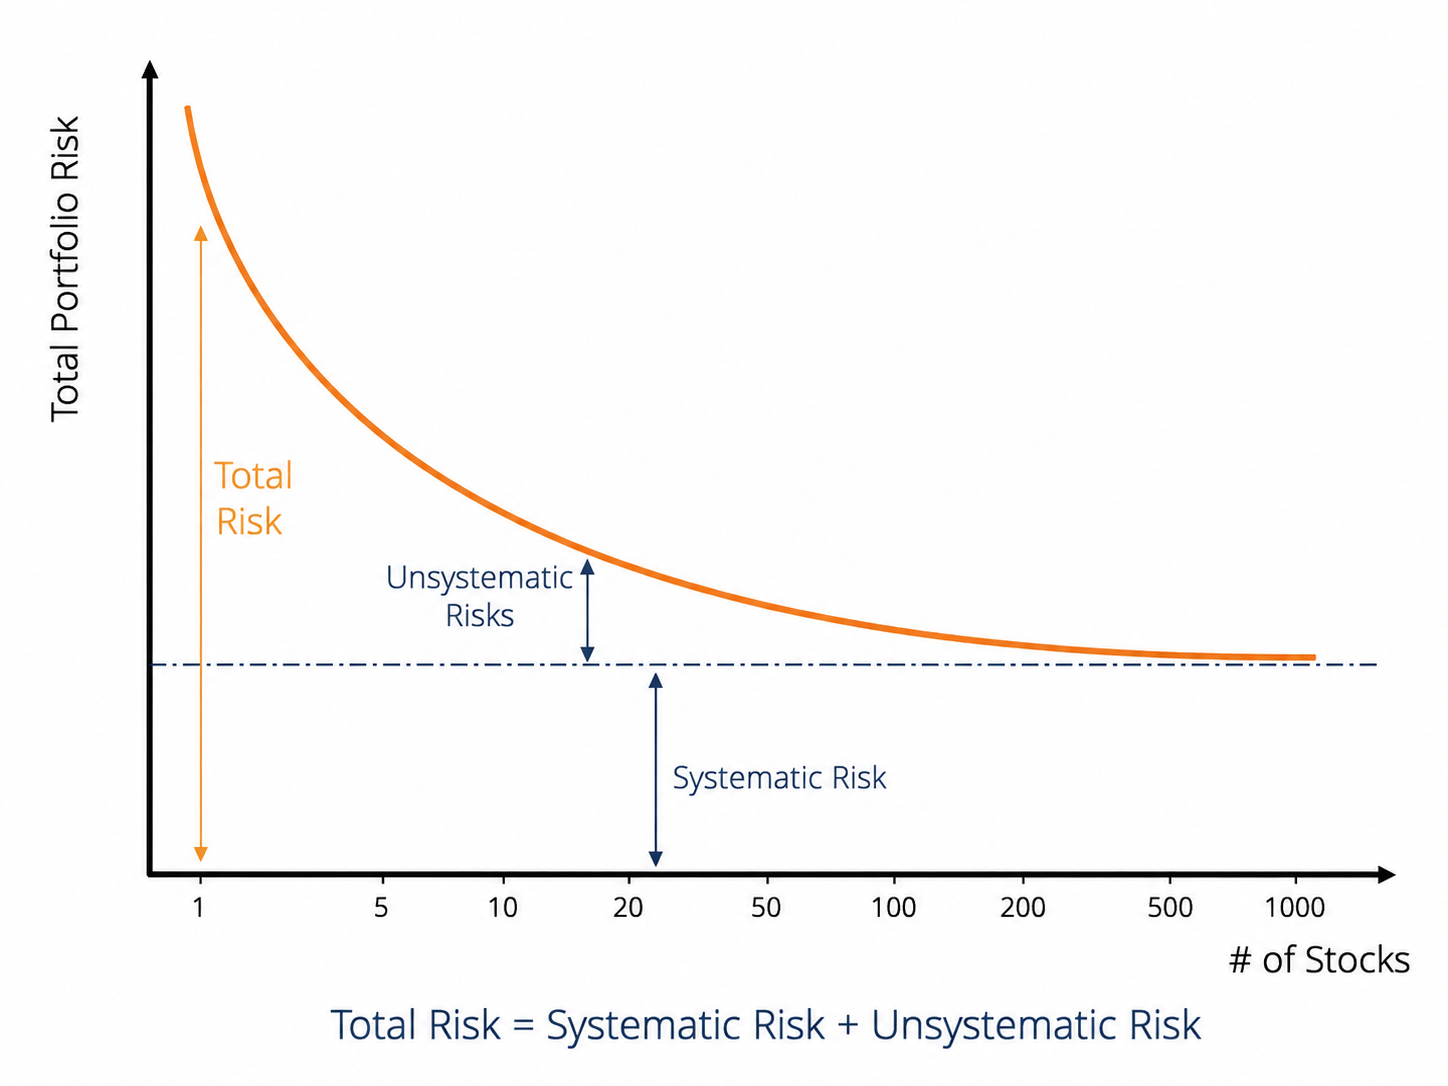
\includegraphics[keepaspectratio]{1-quantitative-finance/figures/diversification.png}}

}

\caption{\label{fig-diversification}Decomposition of total risk into
systematic and diversifiable risk as assets are progressively added to a
portfolio.}

\end{figure}%

This distinction has a fundamental implication for asset pricing. In a
competitive market, rational investors should not expect compensation
for taking risks that can be eliminated at virtually no cost through
diversification. As a result, the market only rewards exposure to
systematic risk. This idea forms the conceptual foundation of the CAPM,
which states that the expected risk premium of an asset should be
proportional to the expected risk premium of the market
\citeproc{ref-sharpe1964capital}{{[}2{]}}
\citeproc{ref-lintner1975valuation}{{[}3{]}}:

\begin{equation}\phantomsection\label{eq-capm}{
\mathbb{E}[r_i] - r_f = \beta_i \left( \mathbb{E}[r_m] - r_f \right)
}\end{equation}

In this expression, \(\mathbb{E}[r_i]\) represents the expected return
of asset \(i\), \(r_f\) is the risk-free rate, and \(\mathbb{E}[r_m]\)
corresponds to the expected return of the market portfolio. The
parameter \(\beta_i\) measures the sensitivity of the asset to market
fluctuations and summarizes its exposure to systematic risk.

From a modeling perspective, the estimation of beta can be interpreted
as a simple linear regression between asset returns and market returns
\citeproc{ref-bossaerts2006lectures}{{[}4{]}}. In this project, the CAPM
is implemented precisely under this framework, using simple linear
regression to estimate the market exposure of different assets and
analyze the relationship between systematic risk and expected return.

Despite its conceptual simplicity and historical importance, the CAPM
assumes that the entire structure of systematic risk can be summarized
by a single factor: the market itself. Empirical evidence, however,
suggests that certain firm characteristics --- such as company size or
the relationship between book value and market value --- capture
persistent return patterns that the CAPM does not fully explain. These
observations motivated the development of the multifactor models
proposed by Fama and French \citeproc{ref-fama1993common}{{[}5{]}}
\citeproc{ref-fama1997industry}{{[}6{]}}.

In this project, these extensions are implemented using multiple linear
regression. The three-factor model can be expressed as:

\begin{equation}\phantomsection\label{eq-fama-french-3factor}{
\mathbb{E}[r_i] - r_f = \alpha + \beta_{mkt} (\mathbb{E}[r_m] - r_f) + \beta_{smb} \cdot \text{SMB} + \beta_{hml} \cdot \text{HML} + \varepsilon
}\end{equation}

where \(\text{SMB}\) (\emph{Small Minus Big}) measures the excess return
of small-cap stocks relative to large-cap stocks, while \(\text{HML}\)
(\emph{High Minus Low}) captures the return differential between value
and growth stocks \citeproc{ref-brealey2011principles}{{[}7{]}}
\citeproc{ref-lewinson2022python}{{[}8{]}}.

From a modeling perspective, the transition from the CAPM to the
Fama--French three-factor model can be interpreted as moving from a
simple linear regression to a multiple linear regression framework,
incorporating additional explanatory variables to capture dimensions of
systematic risk that a single-factor model cannot fully represent.

The main objective of the project is not simply to compare statistical
goodness-of-fit metrics, but to understand how different economic
factors contribute to the generation of returns in financial markets and
to evaluate how effectively models of different complexity levels
represent that underlying process.

\section{Methodology and
Implementation}\label{methodology-and-implementation}

\subsection{Data Collection and
Preprocessing}\label{data-collection-and-preprocessing}

The analysis uses daily adjusted closing prices obtained from Yahoo
Finance for both Apple Inc.~(\texttt{AAPL}) and the S\&P 500 index
(\texttt{\^{}GSPC}). The S\&P 500 is used as a proxy for the market
portfolio within the CAPM framework.

The selected period spans from January 2020 to December 2024, providing
a multi-year sample that includes different market conditions and
volatility regimes. Adjusted prices are used in order to account for
corporate actions such as stock splits and dividend adjustments when
available.

After downloading the data, both time series are merged into a single
dataset and aligned by trading date. Missing observations are removed
prior to return calculation.

The price series are initially inspected to verify data consistency and
to obtain a preliminary view of the market dynamics during the analyzed
period.

\begin{figure}

\centering{

\pandocbounded{
\includegraphics[keepaspectratio]{1-quantitative-finance/../notebooks-and-scripts/1-quantitative-finance/1-capm-and-fama-french-factor-model/r/1-capm-model-figures/closing-prices.png}}

}

\caption{\label{fig-capm-closing-prices}Adjusted closing prices for
Apple Inc.~and the S\&P 500 index between 2020 and 2024. The figure is
mainly used as a preliminary inspection of the downloaded financial time
series before return calculation.}

\end{figure}%

Daily simple returns are then computed from the adjusted closing prices.
These returns constitute the main variables used throughout the
regression analysis.

Before estimating the model, the relationship between asset and market
returns is visually explored through a scatter plot. As shown in
Figure~\ref{fig-capm-daily-returns-scatter}, the data already suggest a
positive linear relationship between Apple returns and market returns,
supporting the use of a linear regression framework for the CAPM
estimation.

\begin{figure}

\centering{

\pandocbounded{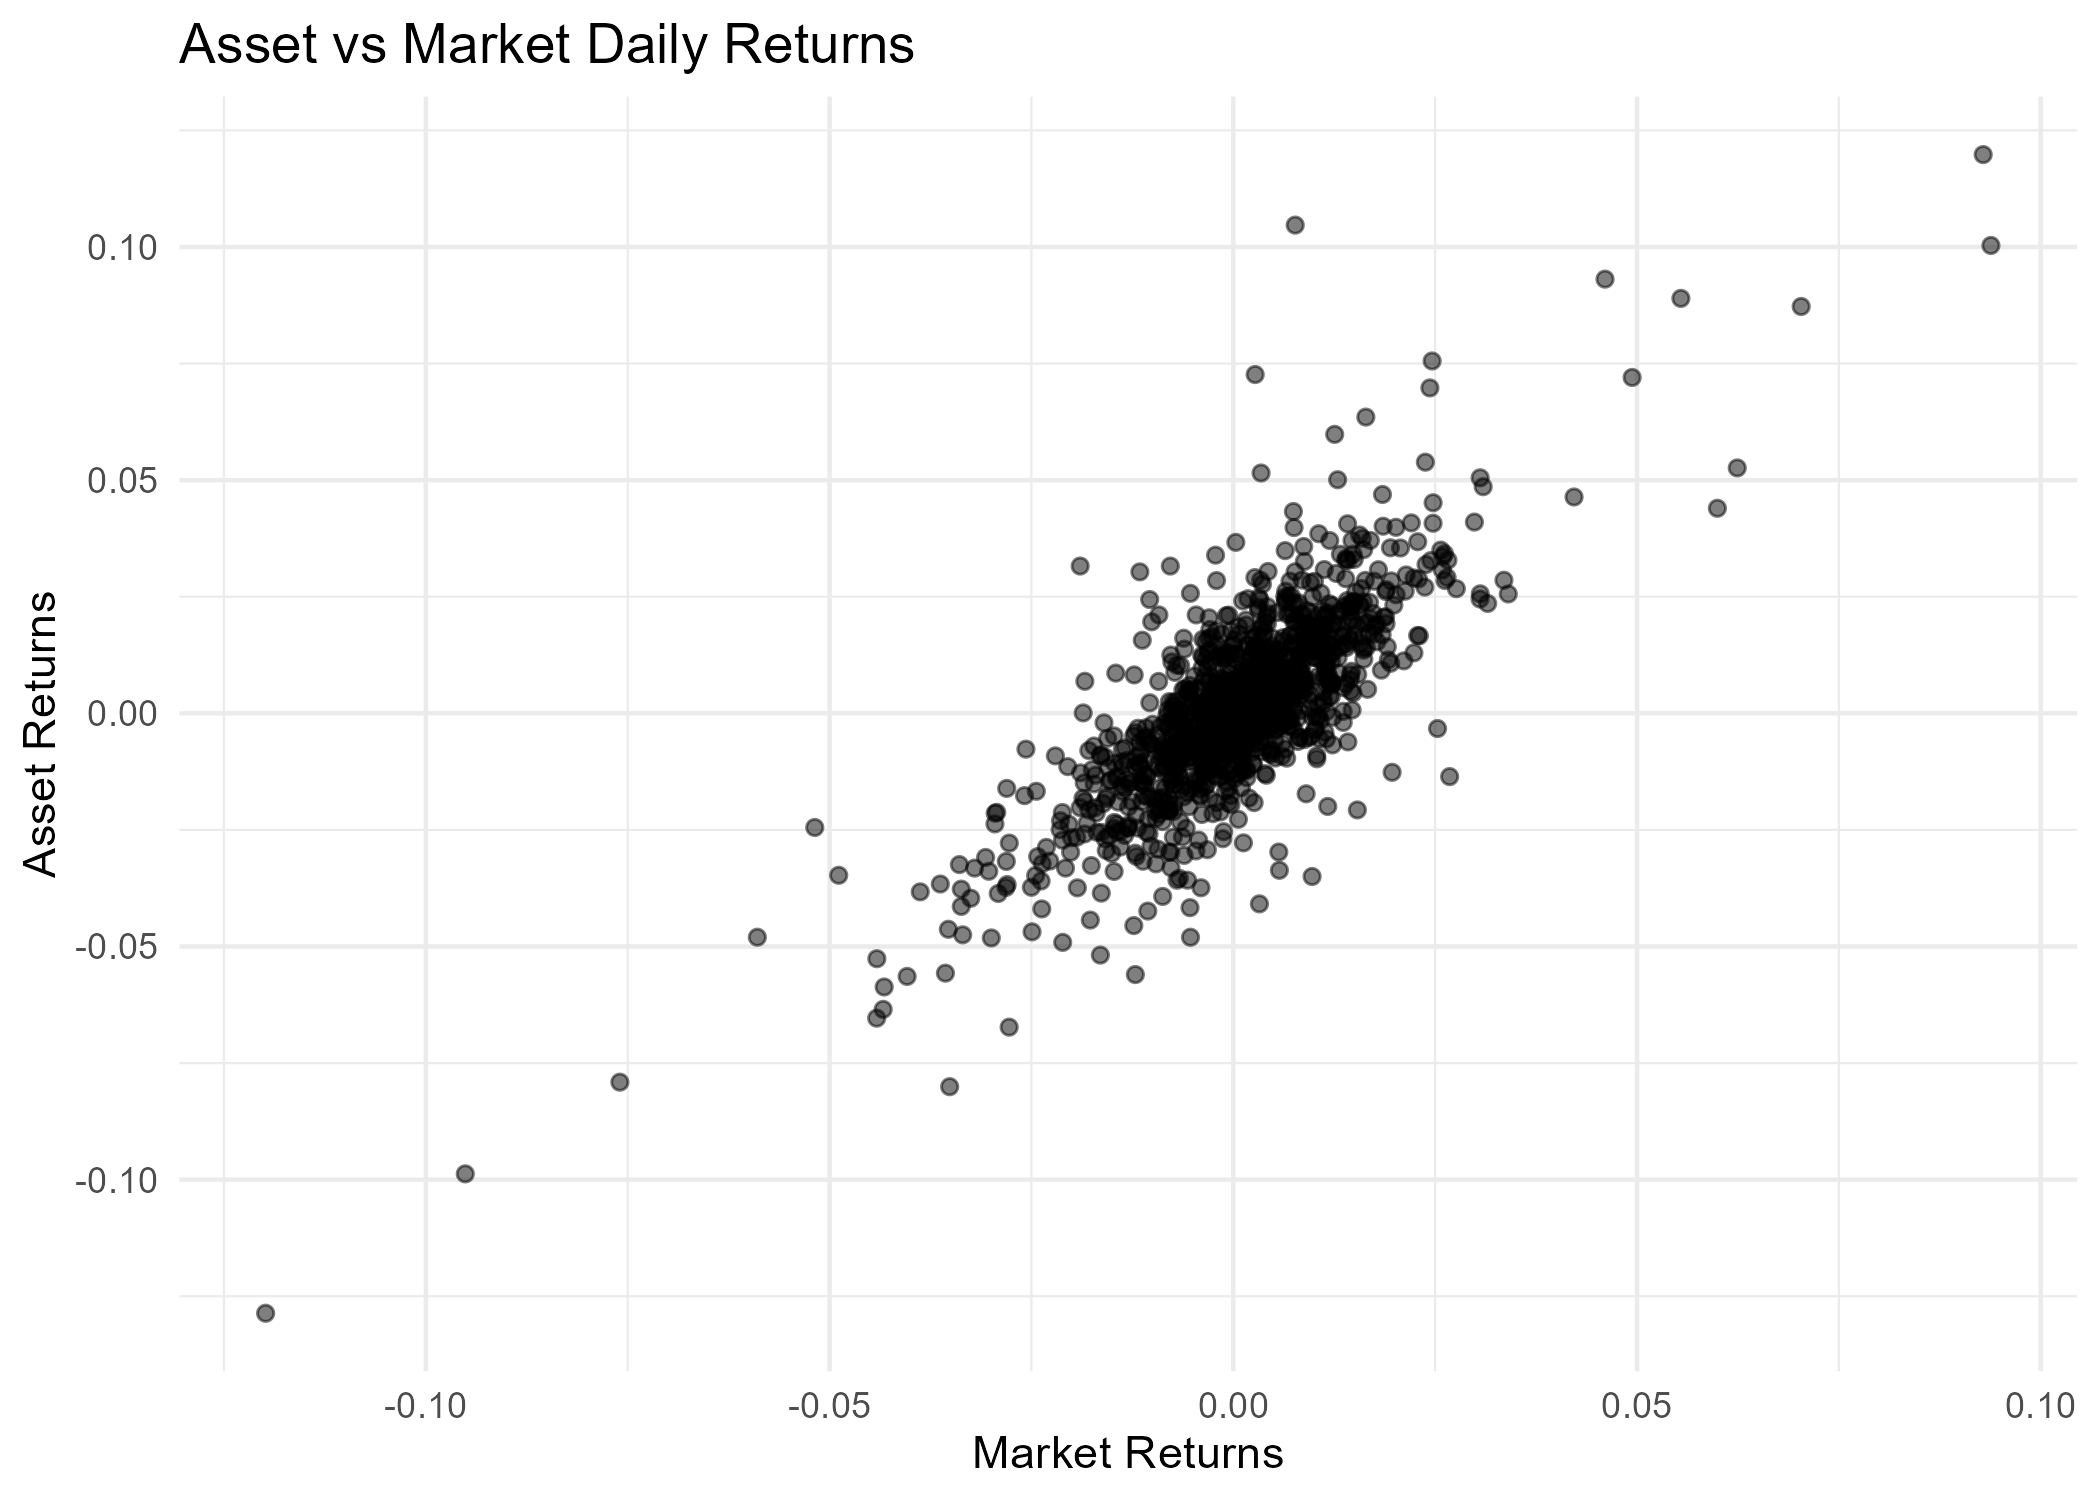
\includegraphics[keepaspectratio]{1-quantitative-finance/../notebooks-and-scripts/1-quantitative-finance/1-capm-and-fama-french-factor-model/r/1-capm-model-figures/daily-returns-scatter.png}}

}

\caption{\label{fig-capm-daily-returns-scatter}Scatter plot of daily
Apple returns against S\&P 500 daily returns. The figure provides an
exploratory visualization of the positive relationship between the asset
and market returns prior to the CAPM estimation.}

\end{figure}%

\subsection{CAPM Implementation}\label{capm-implementation}

Following the theoretical formulation introduced in
Equation~\ref{eq-capm}, the CAPM is implemented through a simple linear
regression in which the daily returns of Apple Inc.~are modeled as a
function of the daily returns of the market portfolio.

For simplicity, the implementation presented here uses raw daily returns
without explicitly incorporating a risk-free rate. Under this
approximation, the model estimates the linear sensitivity of the
selected asset relative to market movements.

The estimated regression coefficients are summarized below.

\begin{longtable}[]{@{}lrrrr@{}}
\caption{Estimated CAPM regression coefficients for Apple Inc.~using the
S\&P 500 as the market
proxy.}\label{tbl-capm-coefficients}\tabularnewline
\toprule\noalign{}
Term & Estimate & Std. Error & t-statistic & p-value \\
\midrule\noalign{}
\endfirsthead
\toprule\noalign{}
Term & Estimate & Std. Error & t-statistic & p-value \\
\midrule\noalign{}
\endhead
\bottomrule\noalign{}
\endlastfoot
(Intercept) & 0.000526 & 0.000346 & 1.5226 & 0.128105 \\
market & 1.173257 & 0.025682 & 45.6847 & 0.000000 \\
\end{longtable}

The estimated market beta is approximately \(\beta = 1.173257\),
indicating that Apple exhibited higher sensitivity to market
fluctuations than the S\&P 500 during the analyzed period. Under the
CAPM interpretation, this coefficient suggests that, on average, Apple
returns moved approximately \(17\%\) more aggressively than the market
portfolio in response to market variations.

Additional model diagnostics are reported below.

\begin{longtable}[]{@{}cc@{}}
\caption{Diagnostic statistics associated with the CAPM linear
regression model.}\label{tbl-capm-diagnostics}\tabularnewline
\toprule\noalign{}
Metric & Value \\
\midrule\noalign{}
\endfirsthead
\toprule\noalign{}
Metric & Value \\
\midrule\noalign{}
\endhead
\bottomrule\noalign{}
\endlastfoot
R-squared & 0.6247 \\
Adjusted R-squared & 0.6244 \\
F-statistic & 2087.0916 \\
Observations & 1256 \\
\end{longtable}

The estimated beta coefficient is also statistically significant, with a
large associated \(t\)-statistic and a near-zero \(p\)-value. Similarly,
the overall regression presents a large \(F\)-statistic, supporting the
existence of a statistically meaningful linear relationship between
Apple returns and market returns during the analyzed period.

The estimated coefficient of determination of approximately
\(R^2 = 0.625\) indicates that the market factor alone explains a
substantial fraction of the observed variability in Apple daily returns
during the selected period. Nevertheless, a significant portion of the
variability remains unexplained, motivating the consideration of
multifactor extensions beyond the single-factor CAPM specification.

The fitted linear relationship between asset and market returns is
illustrated in Figure~\ref{fig-capm-regression}.

\begin{figure}

\centering{

\pandocbounded{
\includegraphics[keepaspectratio]{1-quantitative-finance/../notebooks-and-scripts/1-quantitative-finance/1-capm-and-fama-french-factor-model/r/1-capm-model-figures/capm-regression.png}}

}

\caption{\label{fig-capm-regression}CAPM linear regression between Apple
daily returns and S\&P 500 daily returns. The red line represents the
fitted linear relationship estimated through ordinary least squares
regression.}

\end{figure}%

Additional implementation details, including the companion Quarto and
Python notebooks, are available in the project repository
\href{https://github.com/rodrigokang/portfolio/tree/main/notebooks-and-scripts/1-quantitative-finance/1-capm-and-fama-french-factor-model}{\faGithub}

\subsection{Fama--French Three-Factor Model
Implementation}\label{famafrench-three-factor-model-implementation}

To extend the single-factor CAPM specification, the Fama--French
three-factor model introduced in Equation~\ref{eq-fama-french-3factor}
was estimated using ordinary least squares (OLS) regression. In addition
to the market excess return factor, the model incorporates two
additional systematic risk factors associated with firm size
(\texttt{SMB}) and relative valuation (\texttt{HML}).

The implementation combines daily adjusted closing prices for Apple
Inc.~(\texttt{AAPL}) obtained from Yahoo Finance with the daily
Fama--French factor dataset developed by Kenneth French. The final
modeling dataset contains 1,256 daily observations covering the period
from January 2020 to December 2024. The average daily excess return of
Apple over the sample period was approximately \(0.11\%\), with a daily
standard deviation close to \(2.0\%\).

Additional implementation details, including the companion Quarto and
Python notebooks, are available in the project repository
\href{https://github.com/rodrigokang/portfolio/tree/main/notebooks-and-scripts/1-quantitative-finance/1-capm-and-fama-french-factor-model}{\faGithub}

Figure~\ref{fig-fama-french-factor-series} displays the behavior of the
three explanatory factors over time. The series exhibit substantial
short-term variability, particularly during periods of market stress
such as the early stages of the COVID-19 pandemic in 2020. The
\texttt{SMB} factor shows the highest volatility among the three factors
during this period, reflecting the stronger sensitivity of small-cap
firms to abrupt changes in market conditions.

\begin{figure}

\centering{

\pandocbounded{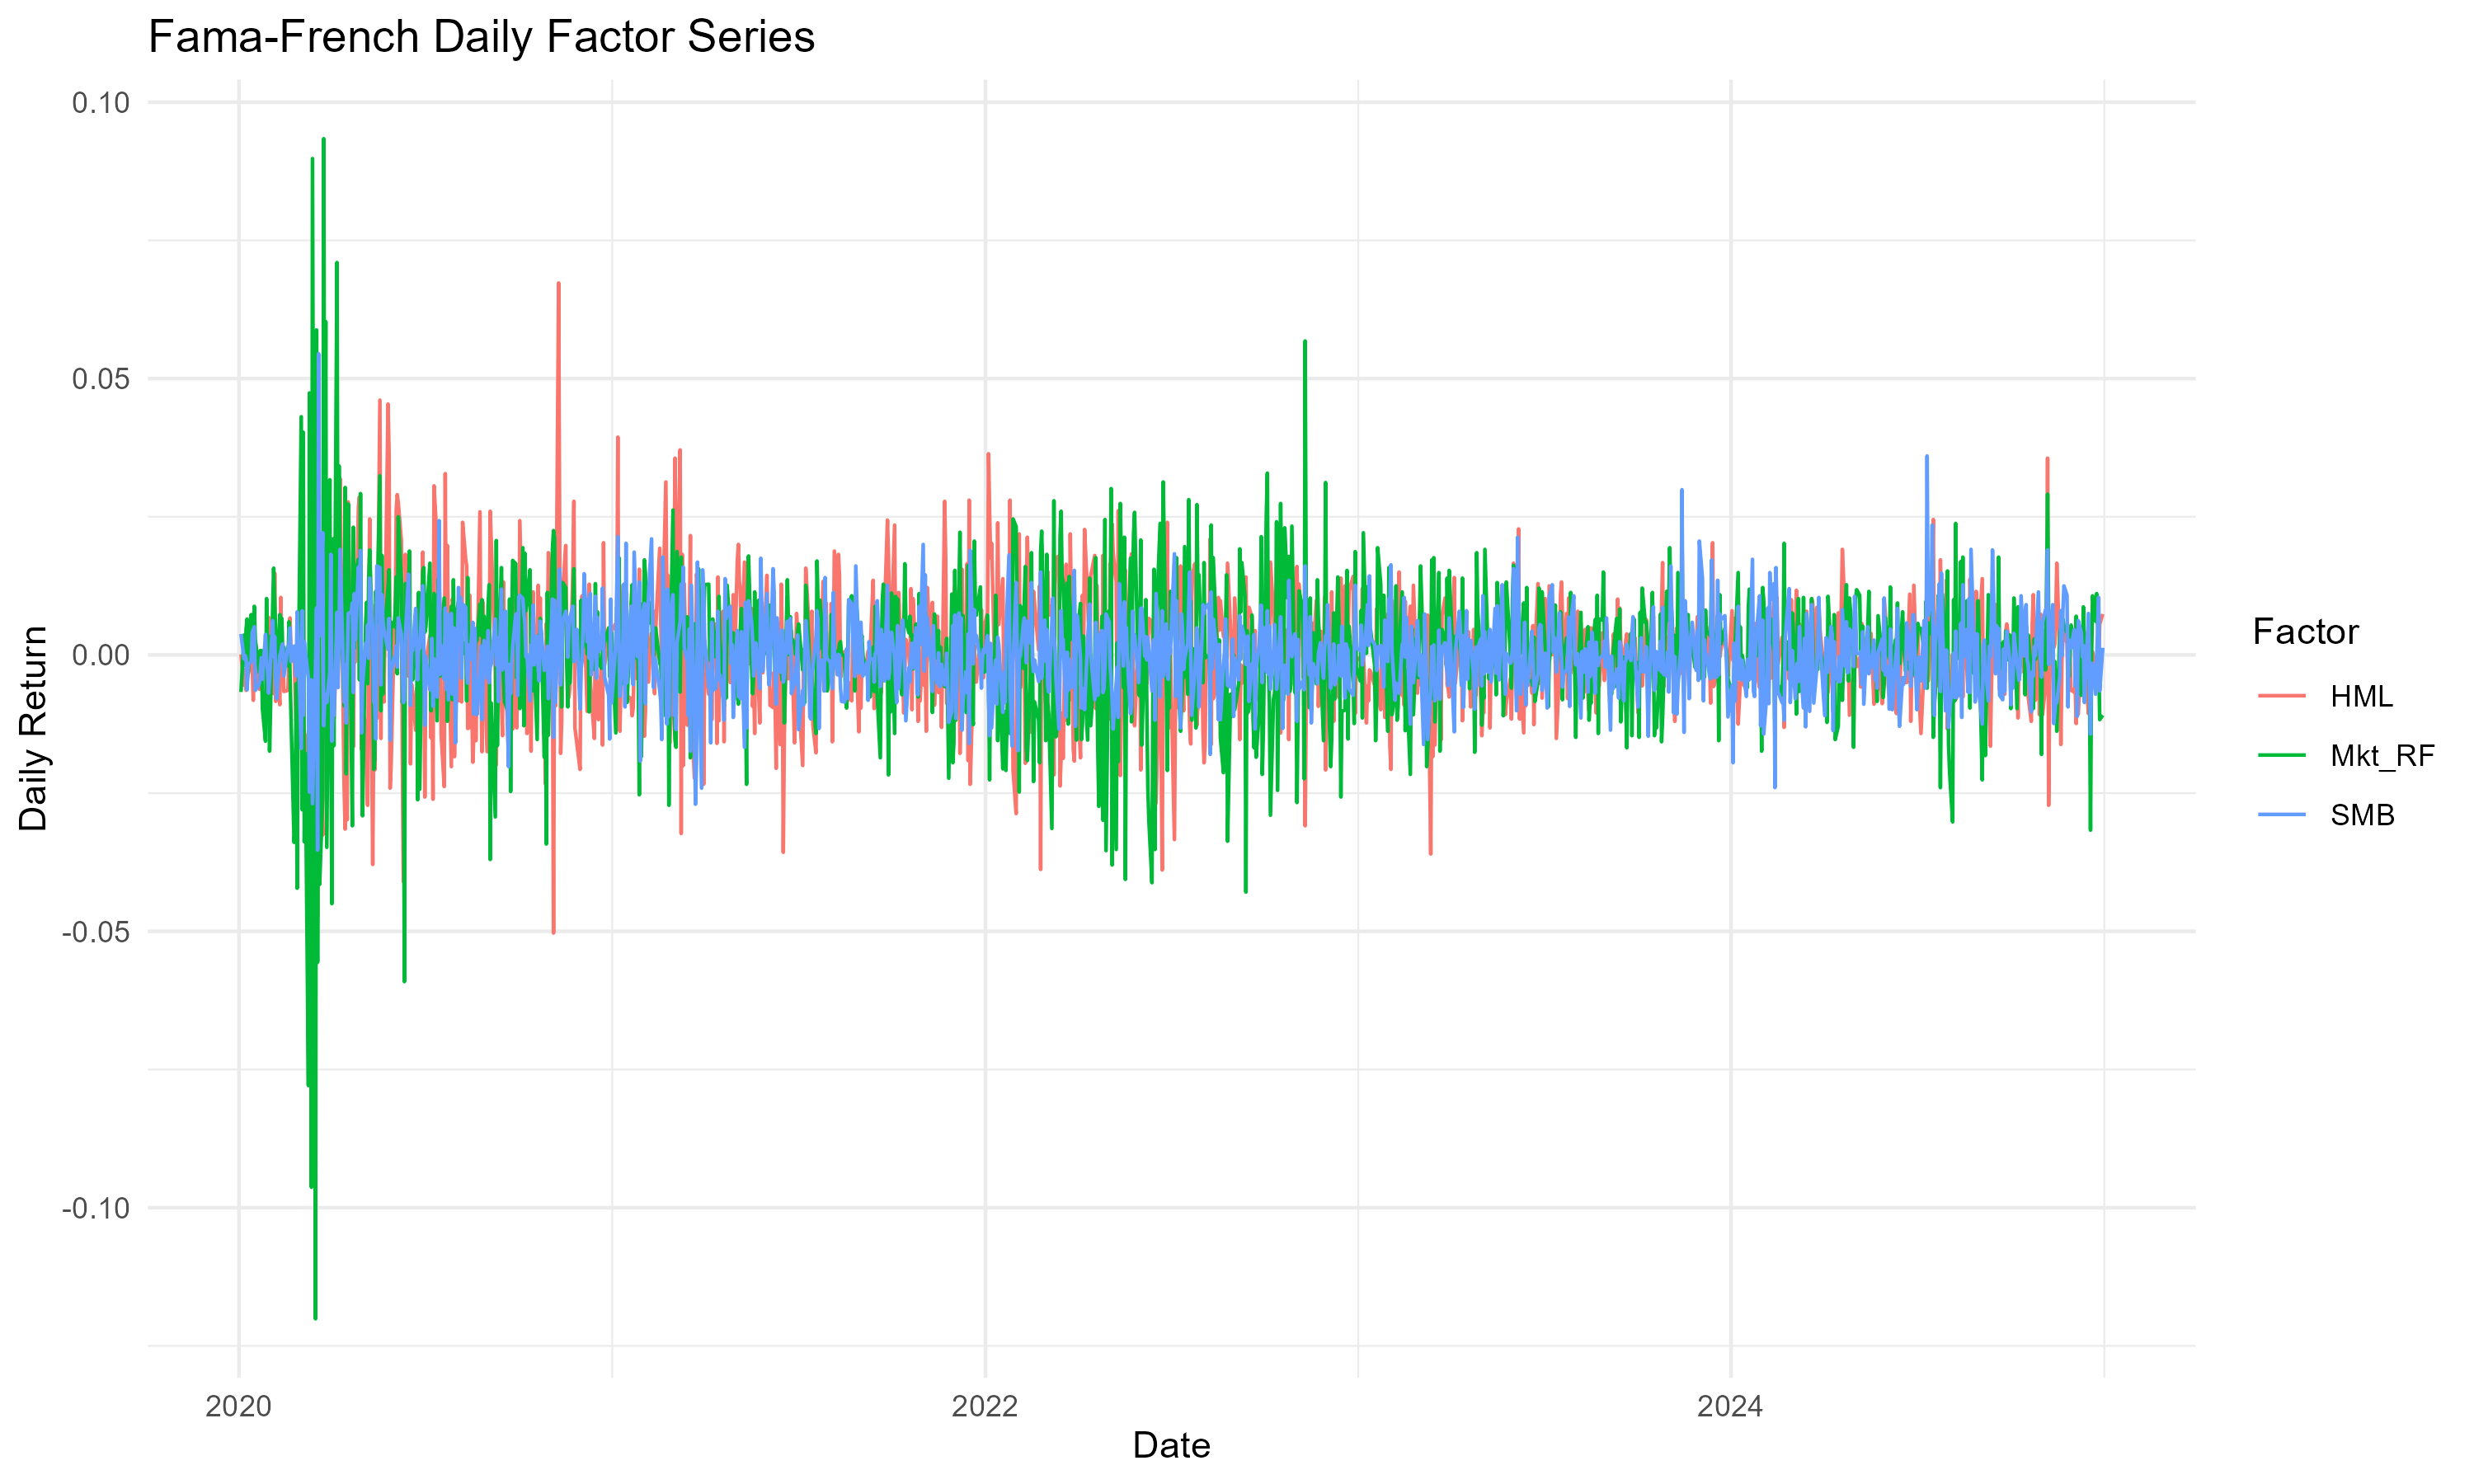
\includegraphics[keepaspectratio]{1-quantitative-finance/../notebooks-and-scripts/1-quantitative-finance/1-capm-and-fama-french-factor-model/r/2-fama-french-three-factor-model-figures/fama_french_factor_series.png}}

}

\caption{\label{fig-fama-french-factor-series}Fama--French daily factor
series.}

\end{figure}%

The estimated regression coefficients are summarized below.

\begin{longtable}[]{@{}
  >{\centering\arraybackslash}p{(\linewidth - 8\tabcolsep) * \real{0.2647}}
  >{\raggedleft\arraybackslash}p{(\linewidth - 8\tabcolsep) * \real{0.1765}}
  >{\raggedleft\arraybackslash}p{(\linewidth - 8\tabcolsep) * \real{0.1912}}
  >{\raggedleft\arraybackslash}p{(\linewidth - 8\tabcolsep) * \real{0.2059}}
  >{\raggedleft\arraybackslash}p{(\linewidth - 8\tabcolsep) * \real{0.1618}}@{}}
\caption{Estimated Fama--French three-factor regression
coefficients.}\label{tbl-ff3-coefficients}\tabularnewline
\toprule\noalign{}
\begin{minipage}[b]{\linewidth}\centering
Term
\end{minipage} & \begin{minipage}[b]{\linewidth}\raggedleft
Estimate
\end{minipage} & \begin{minipage}[b]{\linewidth}\raggedleft
Std. Error
\end{minipage} & \begin{minipage}[b]{\linewidth}\raggedleft
t-statistic
\end{minipage} & \begin{minipage}[b]{\linewidth}\raggedleft
p-value
\end{minipage} \\
\midrule\noalign{}
\endfirsthead
\toprule\noalign{}
\begin{minipage}[b]{\linewidth}\centering
Term
\end{minipage} & \begin{minipage}[b]{\linewidth}\raggedleft
Estimate
\end{minipage} & \begin{minipage}[b]{\linewidth}\raggedleft
Std. Error
\end{minipage} & \begin{minipage}[b]{\linewidth}\raggedleft
t-statistic
\end{minipage} & \begin{minipage}[b]{\linewidth}\raggedleft
p-value
\end{minipage} \\
\midrule\noalign{}
\endhead
\bottomrule\noalign{}
\endlastfoot
Alpha & 0.000455 & 0.000320 & 1.421686 & 0.155366 \\
Market Factor & 1.162676 & 0.024001 & 48.442699 & 0.000000 \\
Size Factor & -0.329641 & 0.042313 & -7.790601 & 0.000000 \\
Value Factor & -0.370591 & 0.027910 & -13.278185 & 0.000000 \\
\end{longtable}

The estimated market beta is approximately \(\beta_{mkt} = 1.163\),
indicating that Apple exhibits a stronger sensitivity to systematic
market movements than the market portfolio itself. The coefficients
associated with the size and value factors are both negative and
statistically significant. The negative loading on \texttt{SMB} suggests
that Apple behaves more similarly to large-cap firms than to small-cap
firms, which is consistent with its market capitalization and dominant
position within the technology sector. Likewise, the negative
\texttt{HML} exposure indicates characteristics more closely aligned
with growth-oriented firms rather than value stocks.

The estimated intercept term (\(\alpha \approx 0.00046\)) is positive
but not statistically significant at conventional significance levels
(\(p \approx 0.155\)), suggesting that, after accounting for the three
systematic risk factors, the model does not provide strong evidence of
abnormal excess returns during the analyzed period.

The overall regression fit improved relative to the single-factor CAPM
specification. The coefficient of determination increased to
approximately \(R^2 = 0.678\), indicating that the three-factor model
explains nearly \(68\%\) of the variability observed in Apple excess
returns. The F-statistic associated with the regression is also highly
significant, supporting the joint explanatory power of the selected
factors.

\begin{longtable}[]{@{}cc@{}}
\caption{Diagnostic statistics associated with the Fama-French
three-factor regression
model.}\label{tbl-ff3-diagnostics}\tabularnewline
\toprule\noalign{}
Metric & Value \\
\midrule\noalign{}
\endfirsthead
\toprule\noalign{}
Metric & Value \\
\midrule\noalign{}
\endhead
\bottomrule\noalign{}
\endlastfoot
R-squared & 0.677865 \\
Adjusted R-squared & 0.677093 \\
Sigma & 0.011345 \\
F-statistic & 878.191163 \\
p-value & 0.000000 \\
Observations & 1256 \\
\end{longtable}

Figure~\ref{fig-fama-french-observed-fitted} compares the observed
excess returns against the fitted values generated by the regression
model. The fitted series captures a substantial fraction of the
short-term dynamics of Apple returns, although large residual
fluctuations remain during periods of elevated volatility.

\begin{figure}

\centering{

\pandocbounded{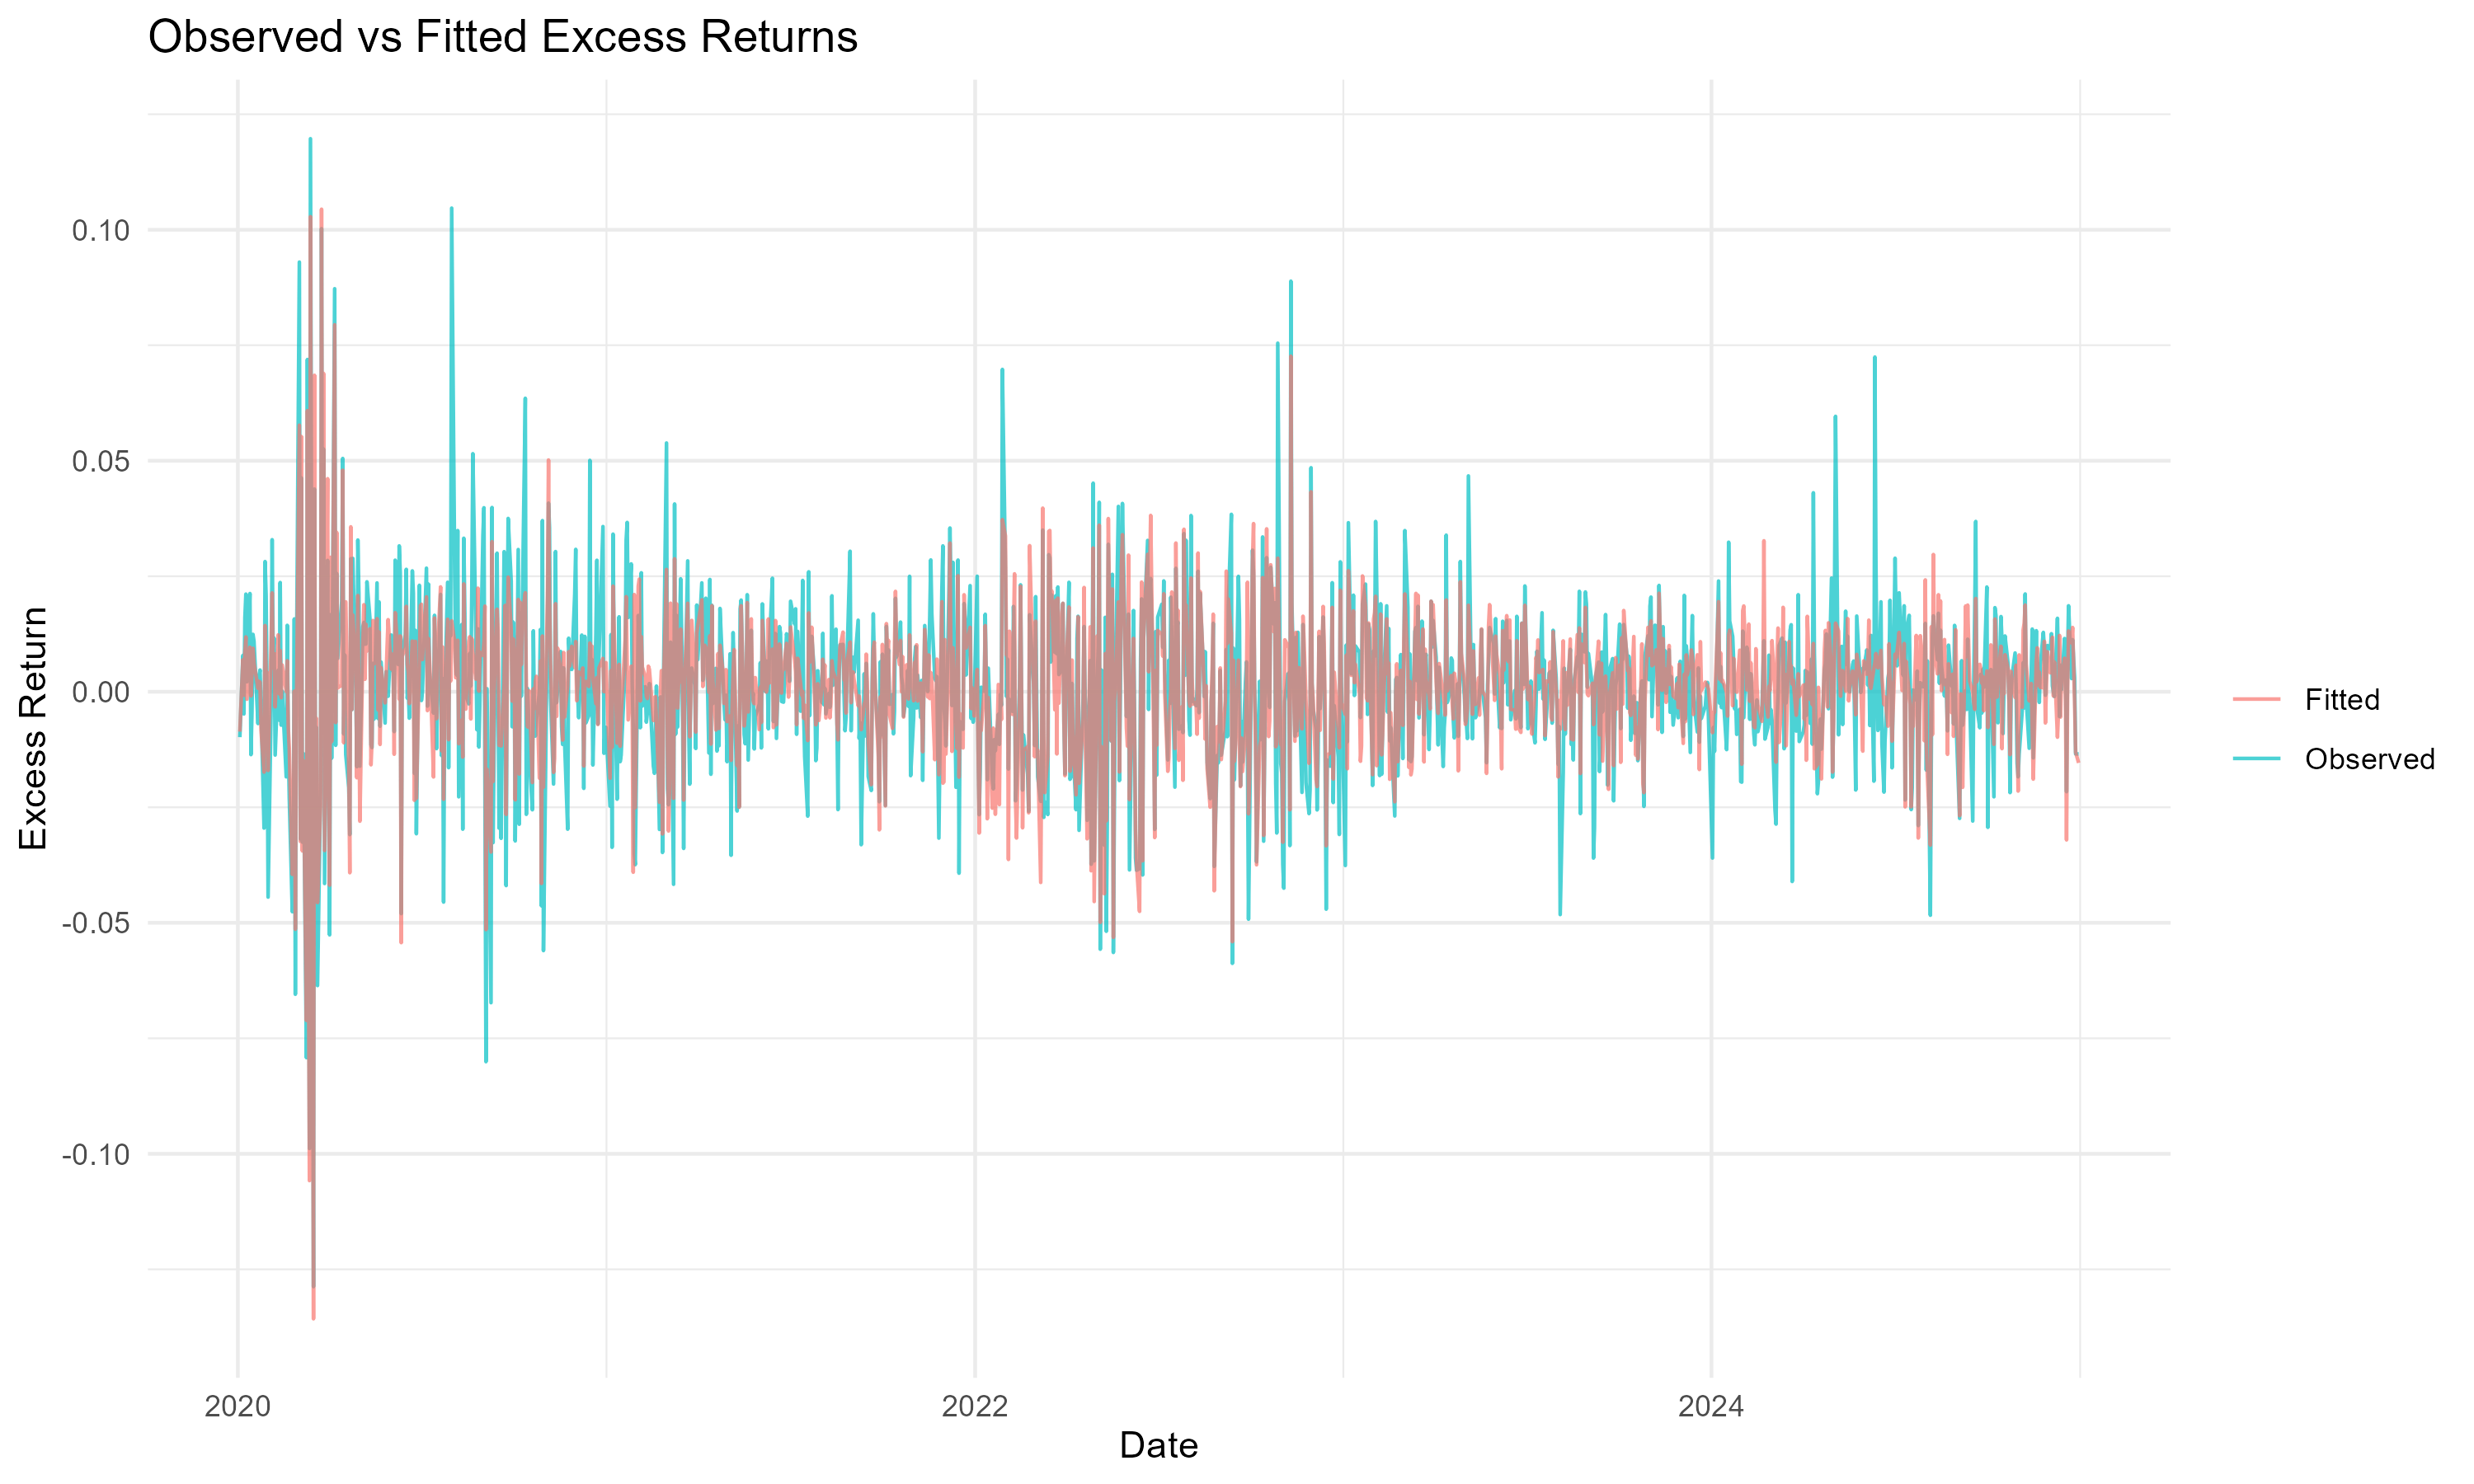
\includegraphics[keepaspectratio]{1-quantitative-finance/../notebooks-and-scripts/1-quantitative-finance/1-capm-and-fama-french-factor-model/r/2-fama-french-three-factor-model-figures/fama_french_observed_vs_fitted_returns.png}}

}

\caption{\label{fig-fama-french-observed-fitted}Observed and fitted
excess returns under the Fama--French three-factor specification.}

\end{figure}%

The residual series displayed in Figure~\ref{fig-fama-french-residuals}
remains approximately centered around zero throughout the analyzed
period, without obvious long-term structural drift. However, clusters of
higher residual volatility are still visible during stressed market
conditions, indicating that a portion of the variability remains
unexplained even after incorporating the additional systematic factors.

\begin{figure}

\centering{

\pandocbounded{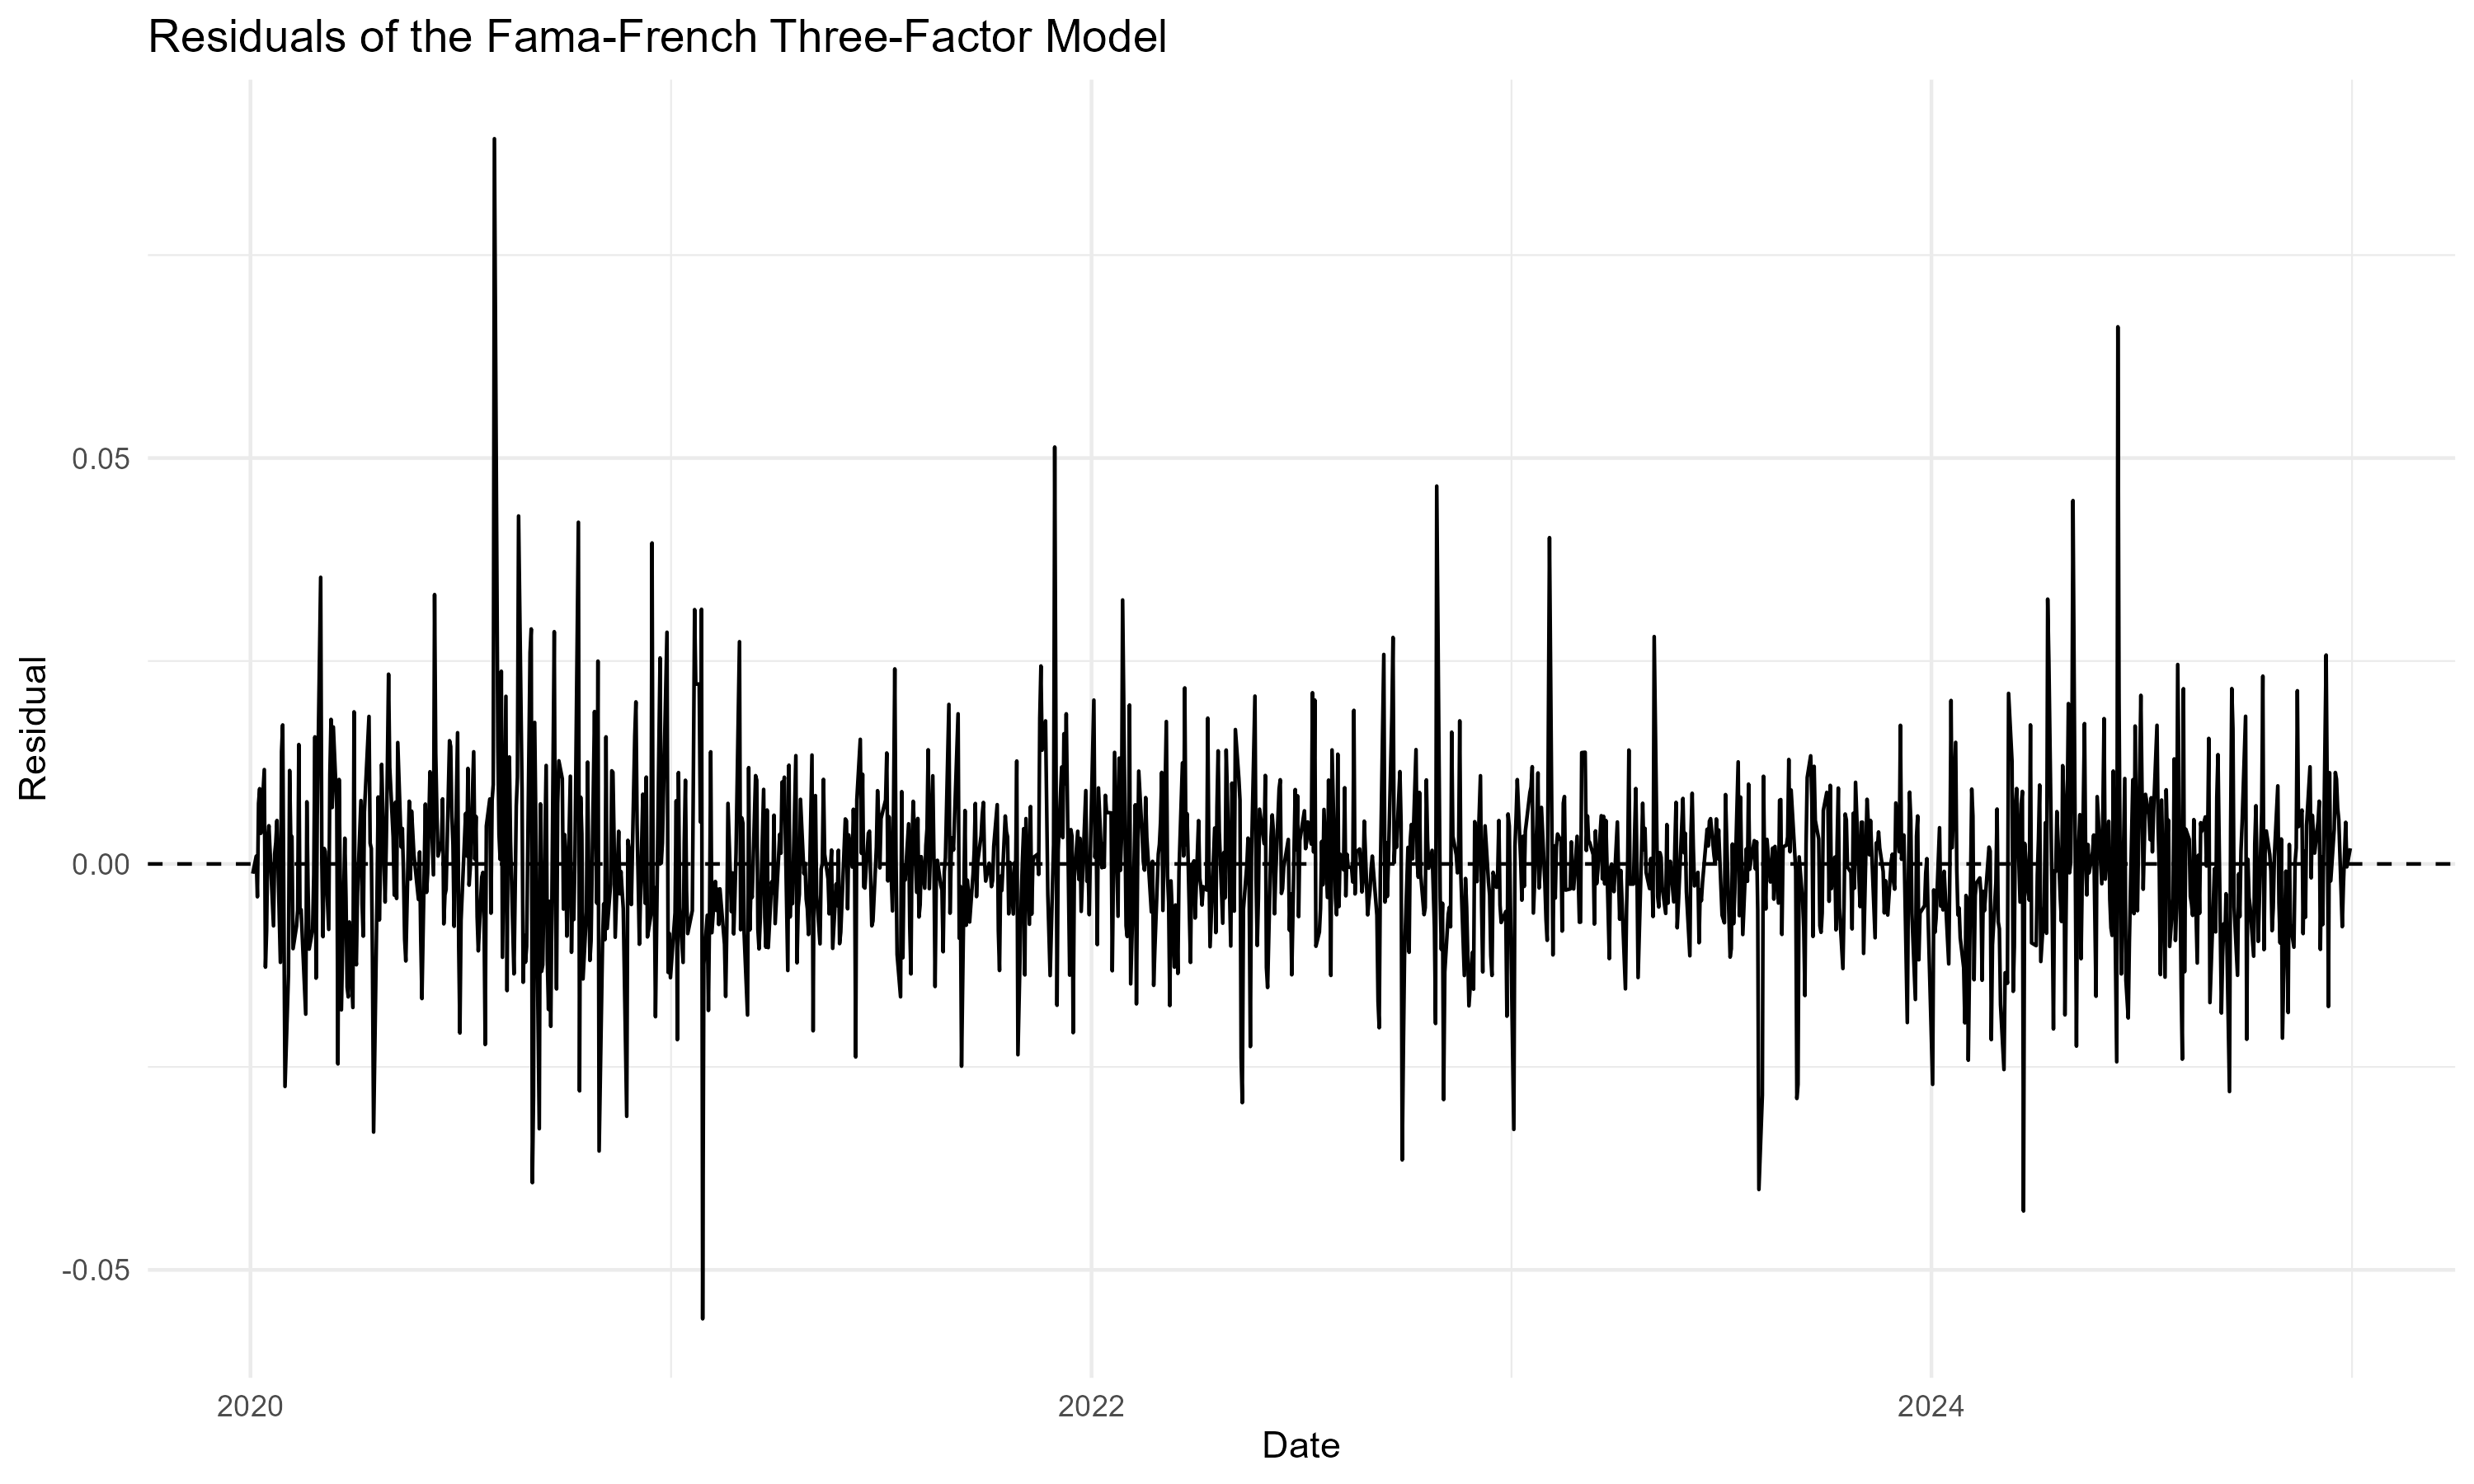
\includegraphics[keepaspectratio]{1-quantitative-finance/../notebooks-and-scripts/1-quantitative-finance/1-capm-and-fama-french-factor-model/r/2-fama-french-three-factor-model-figures/fama_french_residuals.png}}

}

\caption{\label{fig-fama-french-residuals}Residual series of the
Fama--French three-factor model.}

\end{figure}%

Finally, the residual distribution shown in
Figure~\ref{fig-fama-french-residual-distribution} exhibits a roughly
symmetric shape centered near zero, although moderate tail behavior
remains visible. This behavior is consistent with the presence of
occasional large market movements that are not fully captured by the
linear factor structure.

\begin{figure}

\centering{

\pandocbounded{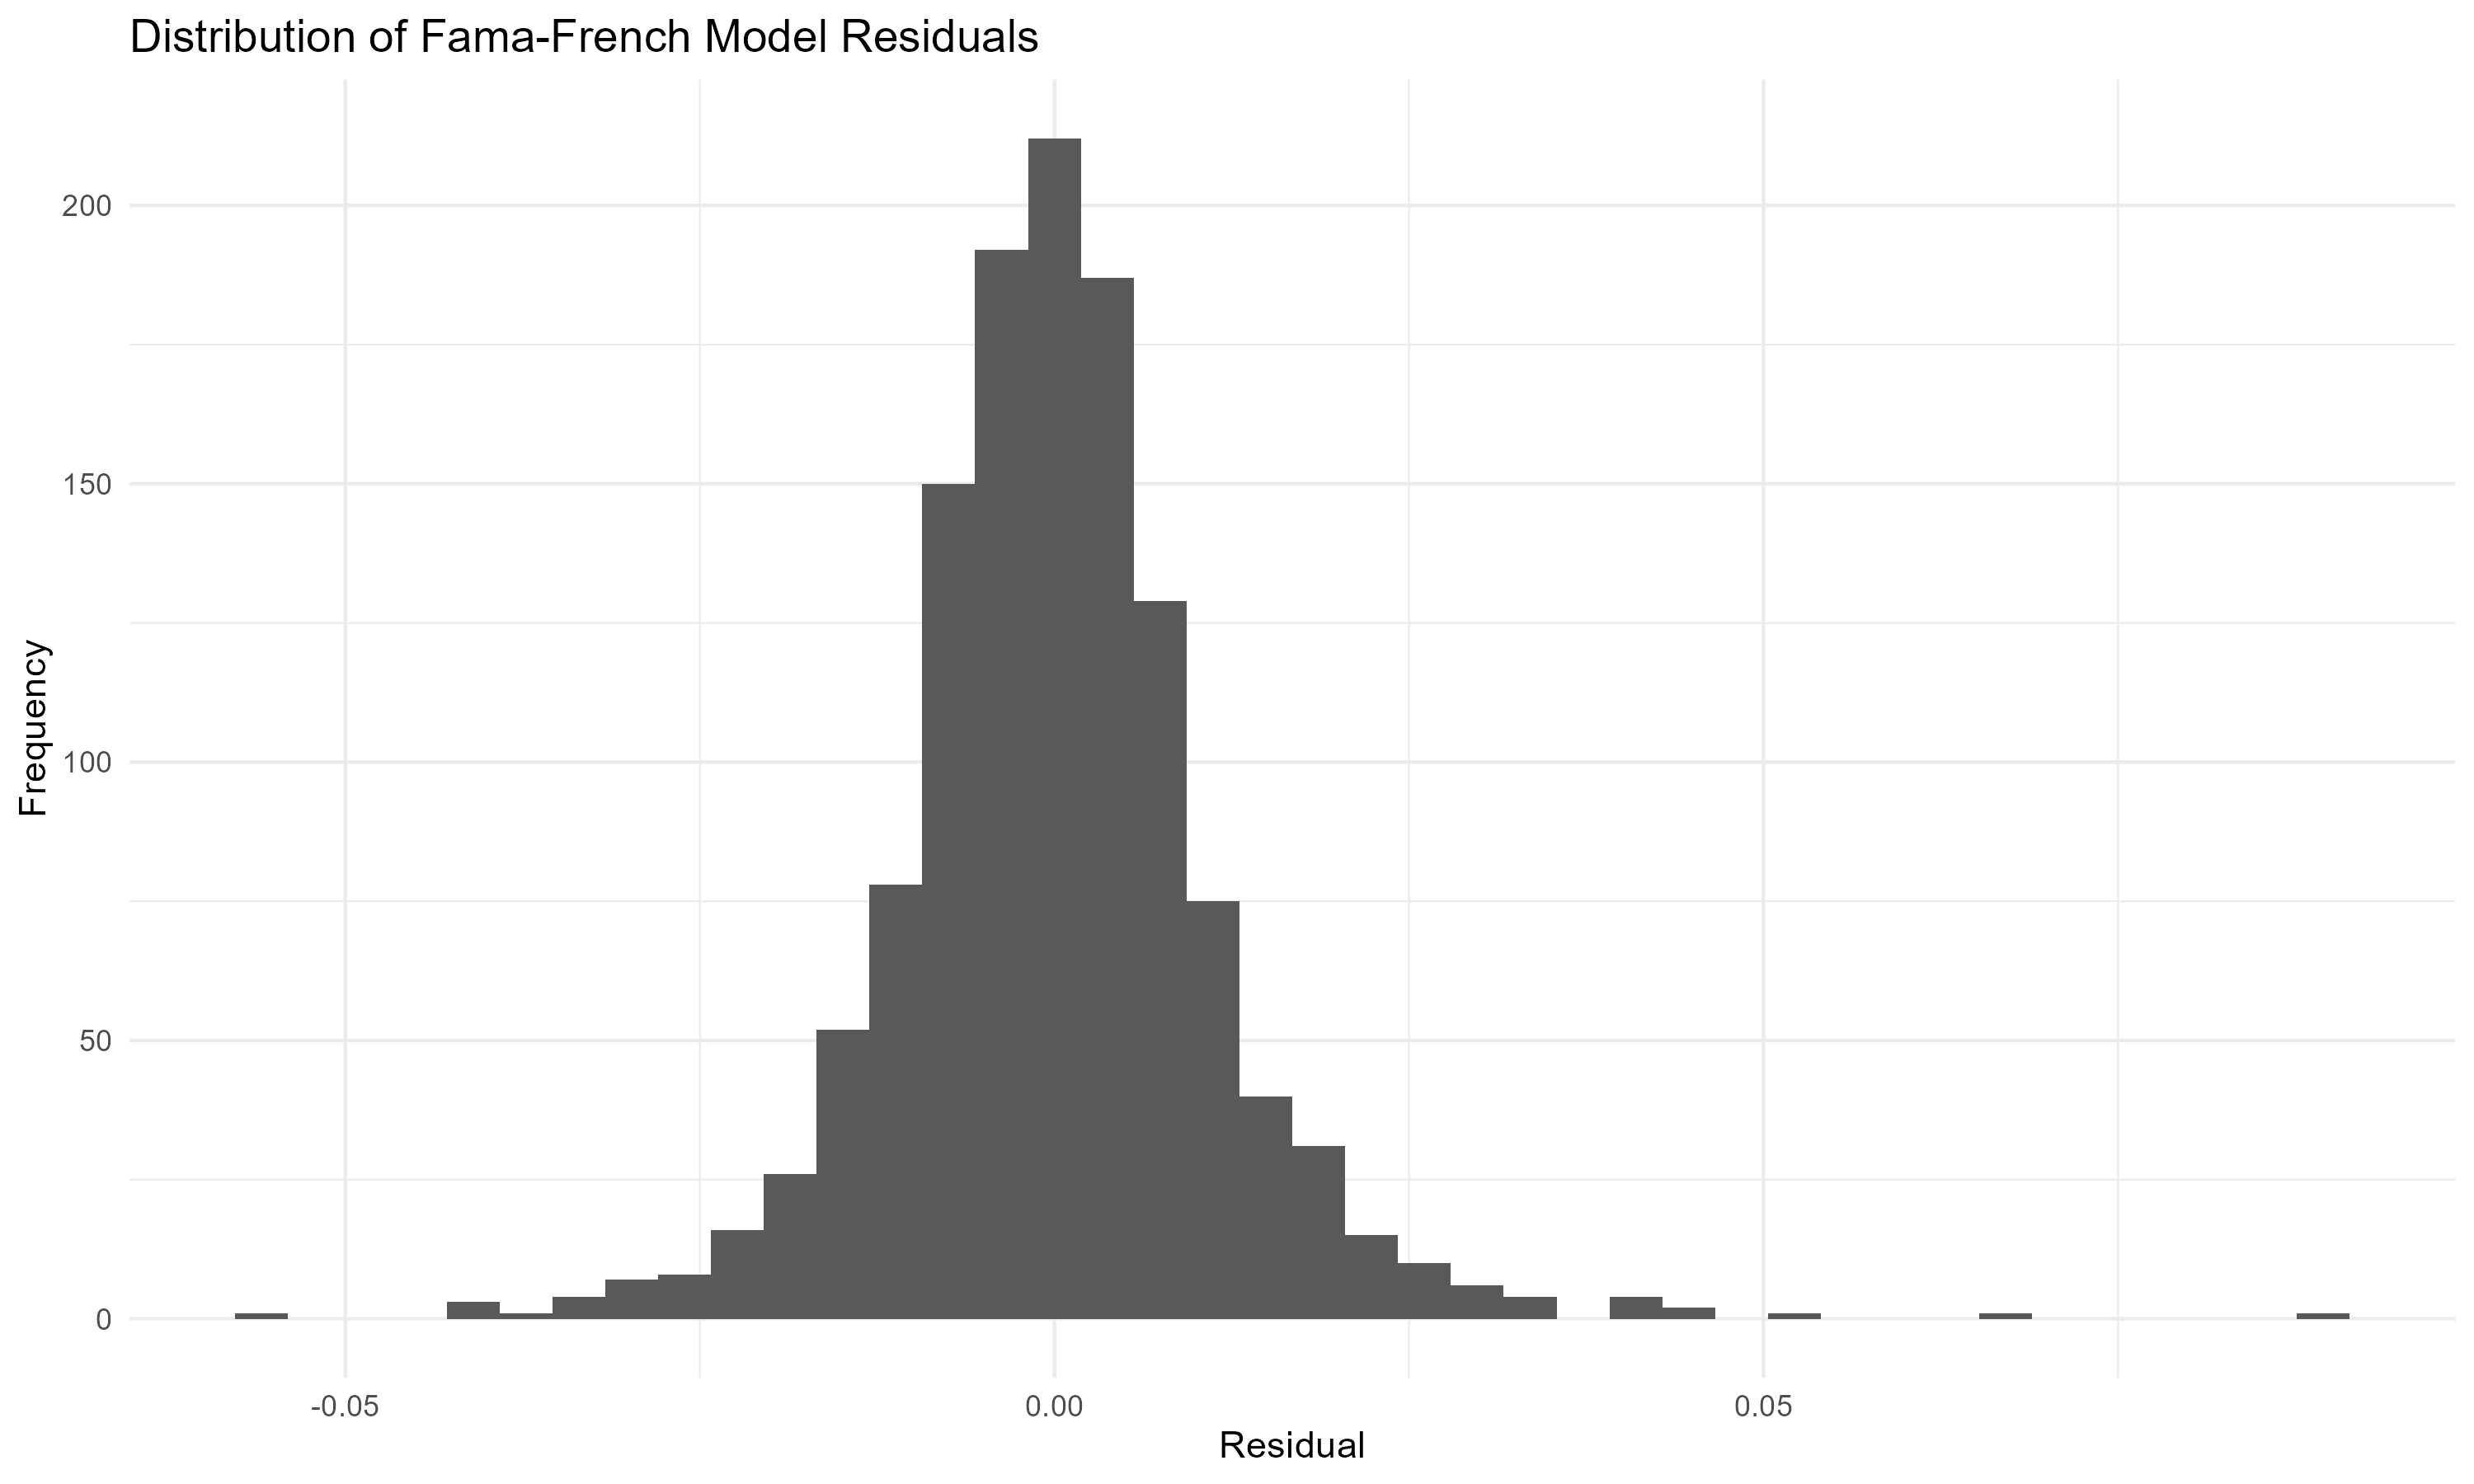
\includegraphics[keepaspectratio]{1-quantitative-finance/../notebooks-and-scripts/1-quantitative-finance/1-capm-and-fama-french-factor-model/r/2-fama-french-three-factor-model-figures/fama_french_residual_distribution.png}}

}

\caption{\label{fig-fama-french-residual-distribution}Distribution of
residuals from the Fama--French three-factor model.}

\end{figure}%

\section{Results, Discussion, and
Limitations}\label{results-discussion-and-limitations}

The empirical results obtained from both the CAPM and the Fama--French
three-factor model provide a useful comparison between single-factor and
multifactor approaches to asset pricing. Although both models capture an
important fraction of the variability observed in Apple excess returns,
the inclusion of additional systematic risk factors in the Fama--French
specification produces a measurable improvement in explanatory
performance.

\subsection{Comparative Analysis}\label{comparative-analysis}

The CAPM estimation produced a market beta close to
\(\beta \approx 1.17\), indicating that Apple exhibits a level of
systematic risk slightly higher than that of the overall market
portfolio. The market factor alone explained approximately \(62.5\%\) of
the variability in Apple excess returns over the analyzed period,
resulting in an estimated coefficient of determination of approximately
\(R^2 = 0.625\).

After incorporating the size (\texttt{SMB}) and value (\texttt{HML})
factors, the explanatory power of the regression increased to
approximately \(R^2 = 0.678\). Although the increase in explanatory
performance is moderate, the multifactor specification captures an
additional fraction of return variability that remains unexplained under
the single-factor CAPM framework.

The estimated market beta remained relatively stable across both models,
suggesting that market risk continues to represent the dominant
systematic component driving Apple returns. However, the additional
factor loadings provide further insight into the firm's structural
characteristics. The negative exposure to the size factor indicates that
Apple behaves more similarly to large-cap firms than to smaller
companies, while the negative loading associated with the value factor
reflects characteristics commonly associated with growth-oriented firms.

From a statistical perspective, both models produced highly significant
overall regressions according to their respective F-statistics.
Nevertheless, the Fama--French specification generated lower residual
variability and a modest improvement in fitted return dynamics,
particularly during periods of elevated market volatility.

The comparison between observed and fitted excess returns also suggests
that the multifactor specification is better able to reproduce
short-term return fluctuations than the CAPM alone. However, significant
residual movements remain visible in both models, indicating that a
substantial fraction of the variability in daily equity returns cannot
be fully captured through linear factor structures alone.

Overall, the empirical results support the interpretation that the
Fama--French three-factor model provides a richer and more flexible
representation of systematic risk exposures relative to the standard
CAPM specification. At the same time, the relatively modest improvement
in explanatory power also highlights the dominant role played by
market-wide risk in large-cap technology firms such as Apple.

\subsection{Model Limitations}\label{model-limitations}

Despite their widespread use in financial economics, both the CAPM and
the Fama--French three-factor model rely on simplifying assumptions that
limit their ability to fully explain observed market behavior.

First, both models assume linear relationships between excess returns
and systematic risk factors. In practice, financial markets frequently
exhibit nonlinear dynamics, volatility clustering, structural breaks,
and regime-dependent behavior that cannot be fully represented within a
static linear regression framework.

Second, the analysis relies on historical daily observations and
therefore assumes that the estimated factor sensitivities remain
relatively stable throughout the selected time horizon. However, the
relationship between individual assets and systematic risk factors may
evolve over time as market conditions, macroeconomic environments, or
firm-specific characteristics change.

An additional limitation arises from the selection of explanatory
factors themselves. Although the Fama--French specification extends the
CAPM by incorporating size and value effects, many additional sources of
systematic risk have been proposed in the literature, including
profitability, investment, momentum, liquidity, and volatility-related
factors. Consequently, the three-factor model should not be interpreted
as a complete description of equity return dynamics.

The analysis also focuses exclusively on a single large-cap technology
company. While Apple represents an interesting case study due to its
market relevance and liquidity, the estimated coefficients and model
diagnostics cannot be directly generalized to other sectors, asset
classes, or market environments without additional empirical validation.

Finally, both models are estimated under the assumption that historical
relationships provide meaningful information regarding future
risk-return behavior. As in most empirical financial applications, this
assumption may fail under changing market conditions, particularly
during periods of financial stress or structural economic transitions.

Despite these limitations, the CAPM and Fama--French frameworks continue
to provide valuable benchmark models for understanding systematic risk
exposures, comparing relative asset sensitivities, and constructing
interpretable factor-based representations of financial returns.

\section{Technical Appendix
(Optional)}\label{technical-appendix-optional}

This appendix provides a compact technical background for the regression
models used in this project. The main body of the chapter focuses on the
financial interpretation of the CAPM and Fama-French models, while this
appendix summarizes the statistical structure underlying their empirical
estimation.

The CAPM specification can be interpreted as a simple linear regression
model, where the excess return of an asset is explained by the excess
return of the market portfolio. In contrast, the Fama-French
three-factor model extends this idea to a multiple linear regression
setting, where asset excess returns are explained by a set of risk
factors rather than by the market factor alone.

The purpose of this appendix is not to provide a complete treatment of
linear regression or statistical learning. Instead, it collects the main
concepts needed to understand how the models were estimated, how the
coefficients should be interpreted, and how goodness-of-fit and
statistical significance measures relate to the empirical results
discussed in the project. The presentation follows standard treatments
of linear regression and statistical learning
\citeproc{ref-james2023statistical}{{[}9{]}}
\citeproc{ref-ugarte2016probability}{{[}10{]}}.

\subsection{Simple Linear Regression and the CAPM
Model}\label{simple-linear-regression-and-the-capm-model}

As discussed previously in Equation~\ref{eq-capm}, the CAPM establishes
a linear relationship between the expected excess return of an asset and
the expected excess return of the market portfolio. From a statistical
perspective, this relationship can be interpreted as a simple linear
regression model of the form

\begin{equation}\phantomsection\label{eq-slr-model}{
y_i = \theta_0 + \theta_1 x_i + \varepsilon_i
}\end{equation}

where \(\theta_0\) represents the intercept, \(\theta_1\) the slope
coefficient, and \(\varepsilon_i\) an unobservable random error
associated with observation \(i\).

Under this interpretation, the empirical CAPM specification can be
written as

\begin{equation}\phantomsection\label{eq-capm-regression}{
r_i - r_f =
\alpha +
\beta(r_m - r_f)
+
\varepsilon
}\end{equation}

where the excess return of the asset plays the role of the response
variable and the excess return of the market portfolio acts as the
predictor variable. In this setting, \(\alpha\) corresponds to the
intercept term, while \(\beta\) measures the sensitivity of the asset
return to market movements.

From the perspective of the CAPM, the intercept term \(\alpha\) is
expected to be equal to zero, implying that expected excess returns are
fully explained by exposure to market risk through the coefficient
\(\beta\). Consequently, testing whether \(\alpha\) differs
significantly from zero provides a practical way to evaluate the
empirical consistency of the model.

\subsubsection{Ordinary Least Squares
Estimation}\label{ordinary-least-squares-estimation}

The parameters of the regression model are estimated by minimizing the
discrepancy between the observed data and the fitted regression line. In
ordinary least squares (OLS), this discrepancy is quantified through the
residual sum of squares (RSS), defined as

\begin{equation}\phantomsection\label{eq-rss}{
\mathrm{RSS}
=
\sum_{i=1}^{N}
(y_i - \hat{y}_i)^2
=
\sum_{i=1}^{N}
(y_i - \theta_0 - \theta_1 x_i)^2
}\end{equation}

where each residual represents the difference between an observed value
and the value predicted by the model.

Figure~\ref{fig-rss} illustrates the geometric interpretation of the
residuals in simple linear regression. The ordinary least squares
estimator selects the parameters that minimize the squared residual
distances between the observations and the fitted regression line.

\begin{figure}

\centering{

\pandocbounded{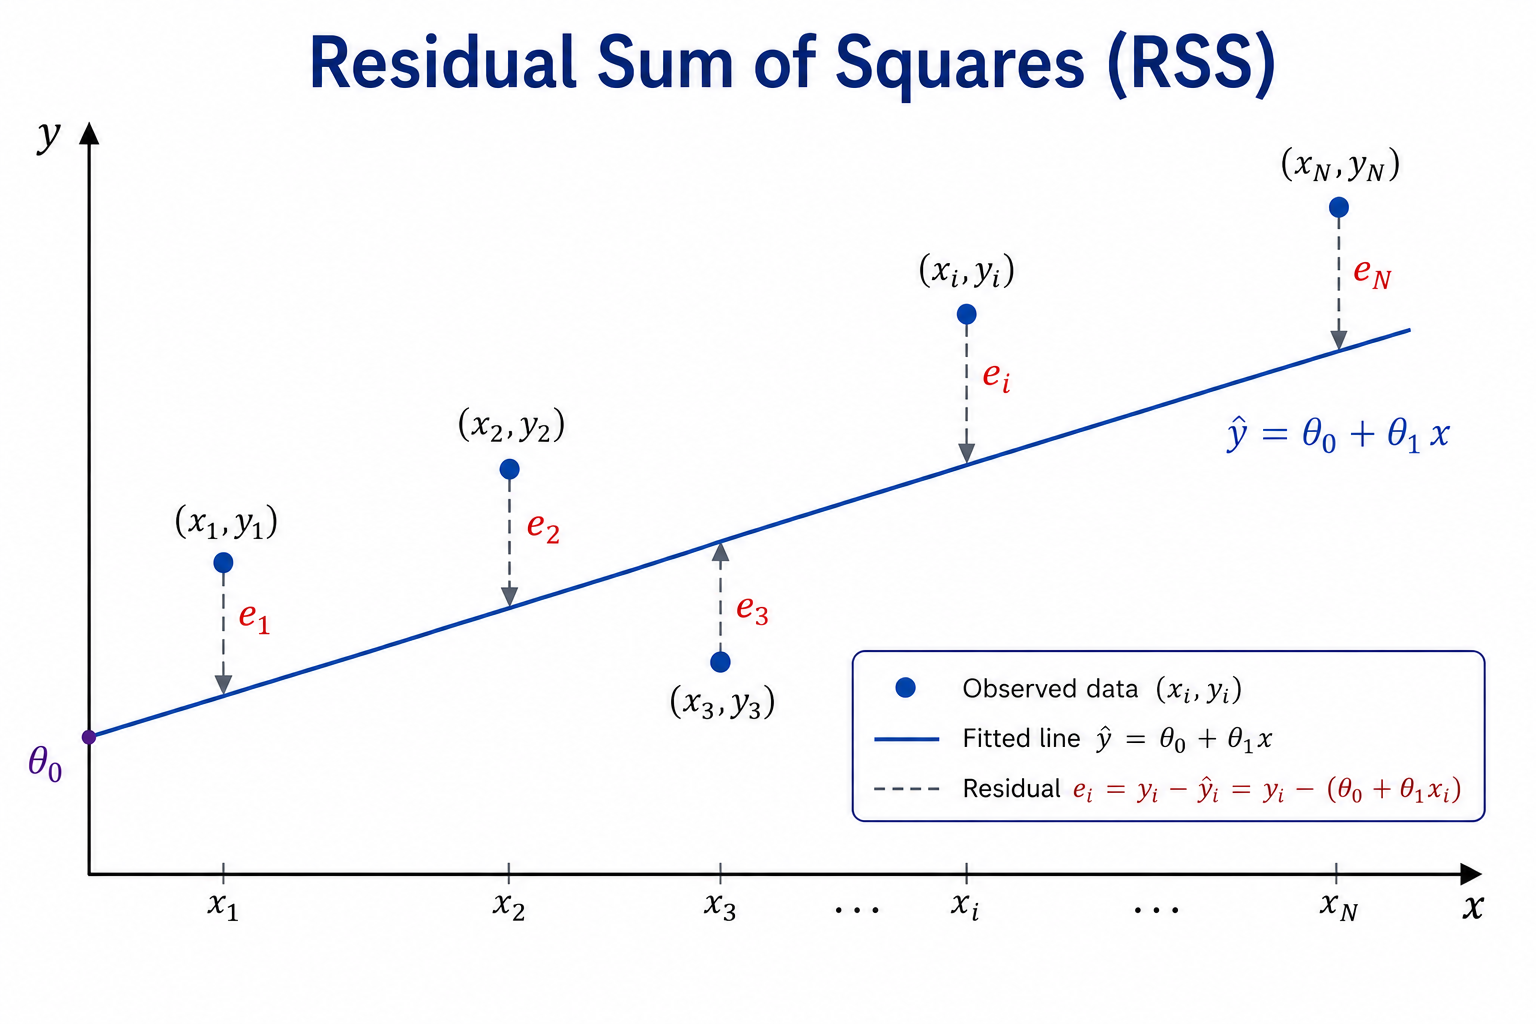
\includegraphics[keepaspectratio]{1-quantitative-finance/figures/rss.png}}

}

\caption{\label{fig-rss}Residual Sum of Squares (RSS)}

\end{figure}%

The ordinary least squares estimators are obtained by minimizing
Equation~\ref{eq-rss} with respect to the model parameters. Since the
RSS is a convex quadratic function of \(\theta_0\) and \(\theta_1\), the
solution can be obtained by setting the gradient equal to zero. The
convexity of the RSS follows from the positive definiteness of the
associated Hessian matrix, ensuring that the stationary point
corresponds to a unique global minimum.

The resulting estimators are given by

\begin{equation}\phantomsection\label{eq-ols-slope}{
\hat{\theta}_1 =
\frac{
\sum_{i=1}^{N}
(x_i - \bar{x})(y_i - \bar{y})
}{
\sum_{i=1}^{N}
(x_i - \bar{x})^2
}
=
\frac{
\mathrm{Cov}(x,y)
}{
\mathrm{Var}(x)
}
}\end{equation}

and

\begin{equation}\phantomsection\label{eq-ols-intercept}{
\hat{\theta}_0
=
\bar{y}
-
\hat{\theta}_1 \bar{x}
}\end{equation}

Equation~\ref{eq-ols-slope} shows that the slope estimator can be
interpreted as the ratio between the covariance of \(x\) and \(y\) and
the variance of \(x\). Consequently, the estimated slope increases when
both variables tend to move together and decreases when their linear
relationship weakens. In the context of empirical asset pricing, this
interpretation leads naturally to the CAPM market beta, which can be
viewed as the ordinary least squares estimator obtained by regressing
the excess return of an asset against the excess return of the market
portfolio. Under this interpretation, the CAPM beta measures the linear
sensitivity of the asset return to market movements in the least-squares
sense.

\subsubsection{Residual Analysis and Model
Assumptions}\label{residual-analysis-and-model-assumptions}

Once the regression coefficients have been estimated, the residuals
provide information about the portion of the variability that is not
explained by the model. For each observation, the residual is defined as

\begin{equation}\phantomsection\label{eq-residuals}{
e_i
=
y_i - \hat{y}_i
}\end{equation}

where \(\hat{y}_i\) denotes the predicted value obtained from the fitted
regression model.

A distinction should be made between residuals and random errors.
Residuals correspond to observable deviations between the fitted model
and the data, whereas the random errors \(\varepsilon_i\) introduced in
Equation~\ref{eq-slr-model} represent the unobservable stochastic
component assumed by the statistical model.

Classical linear regression assumes that the random errors are
independent, centered around zero, and have constant variance. Under
these assumptions,

\begin{equation}\phantomsection\label{eq-gaussian-errors}{
\varepsilon_i
\sim
N(0,\sigma^2)
}\end{equation}

where \(\sigma^2\) denotes the variance of the error term.

The assumption of constant variance is commonly referred to as
homoscedasticity and can be expressed as

\begin{equation}\phantomsection\label{eq-homoscedasticity}{
\mathrm{Var}(\varepsilon_i)
=
\sigma^2
}\end{equation}

for all observations. When the variance of the errors changes across
observations, the model is said to exhibit heteroscedasticity, which may
affect the reliability of confidence intervals, hypothesis tests, and
statistical inference.

Although these assumptions are rarely satisfied exactly in real
financial data, they provide the statistical framework underlying
ordinary least squares estimation and the interpretation of the
inferential quantities discussed in the following sections.

\subsubsection{Confidence Intervals and Standard
Errors}\label{confidence-intervals-and-standard-errors}

The regression coefficients estimated through ordinary least squares are
subject to sampling variability. Consequently, point estimates alone do
not provide information about the uncertainty associated with the
estimated parameters. This uncertainty is commonly quantified through
standard errors and confidence intervals.

Under the assumptions introduced previously, the variance of the random
error term can be estimated from the residuals through the residual
standard error (RSE), defined as

\begin{equation}\phantomsection\label{eq-rse}{
\mathrm{RSE}
=
\sqrt{
\frac{
\mathrm{RSS}
}{
N - 2
}
}
}\end{equation}

where \(N\) denotes the number of observations and the subtraction of
two degrees of freedom reflects the estimation of the intercept and
slope coefficients.

The standard errors associated with the regression coefficients are
given by

\begin{equation}\phantomsection\label{eq-se-slope}{
\mathrm{SE}(\hat{\theta}_1)
=
\sqrt{
\frac{
\sigma^2
}{
\sum_{i=1}^{N}
(x_i - \bar{x})^2
}
}
}\end{equation}

and

\begin{equation}\phantomsection\label{eq-se-intercept}{
\mathrm{SE}(\hat{\theta}_0)
=
\sqrt{
\sigma^2
\left[
\frac{1}{N}
+
\frac{
\bar{x}^2
}{
\sum_{i=1}^{N}
(x_i - \bar{x})^2
}
\right]
}
}\end{equation}

where \(\sigma^2\) is typically replaced in practice by the estimator
introduced in Equation~\ref{eq-rse}.

These expressions show that the uncertainty associated with the
estimated coefficients depends on both the residual variability and the
dispersion of the predictor variable. In particular, the standard error
of the slope coefficient decreases as the variability of \(x\)
increases, leading to more stable estimates of the linear relationship.

Confidence intervals provide a range of plausible values for the
regression coefficients. Under approximate normality assumptions, a
\(95\%\) confidence interval for a parameter \(\theta\) can be written
as

\begin{equation}\phantomsection\label{eq-confidence-interval}{
\hat{\theta}
\pm
2 \cdot \mathrm{SE}(\hat{\theta})
}\end{equation}

indicating the range within which the true parameter value is expected
to lie with approximately \(95\%\) confidence.

\subsubsection{Hypothesis Testing and Statistical
Significance}\label{hypothesis-testing-and-statistical-significance}

Beyond estimating the regression coefficients, it is often important to
evaluate whether the observed linear relationship is statistically
significant. In simple linear regression, this is commonly assessed
through hypothesis testing on the slope coefficient.

The null and alternative hypotheses are given by

\begin{equation}\phantomsection\label{eq-hypothesis-test}{
\begin{cases}
H_0 : \theta_1 = 0 \\
H_1 : \theta_1 \neq 0
\end{cases}
}\end{equation}

Under the null hypothesis, the predictor variable does not contribute to
explaining the variability of the response variable, implying the
absence of a linear relationship between \(x\) and \(y\).

The statistical significance of the estimated slope coefficient can be
evaluated through the t-statistic,

\begin{equation}\phantomsection\label{eq-t-statistic}{
t
=
\frac{
\hat{\theta}_1
}{
\mathrm{SE}(\hat{\theta}_1)
}
}\end{equation}

which measures the magnitude of the estimated coefficient relative to
its standard error.

The corresponding p-value quantifies the probability of observing a
statistic at least as extreme as the one obtained under the null
hypothesis. Small p-values provide evidence against \(H_0\), suggesting
that the predictor variable contributes significantly to the regression
model.

In the context of the CAPM, hypothesis testing is particularly relevant
for evaluating whether the estimated market exposure coefficient differs
significantly from zero and whether the intercept term is statistically
consistent with the theoretical prediction of \(\alpha = 0\).

\subsubsection{Analysis of Variance
(ANOVA)}\label{analysis-of-variance-anova}

The variability of the response variable can be decomposed into a
component explained by the regression model and a residual component
associated with unexplained variability. In simple linear regression,
this decomposition is expressed as

\begin{equation}\phantomsection\label{eq-anova-decomposition-pointwise}{
y_i - \bar{y}
=
(\hat{y}_i - \bar{y})
+
(y_i - \hat{y}_i)
}\end{equation}

which separates the total deviation of each observation into an
explained component and a residual component.

Figure~\ref{fig-anova} illustrates the geometric interpretation of this
decomposition in the context of simple linear regression.

\begin{figure}

\centering{

\pandocbounded{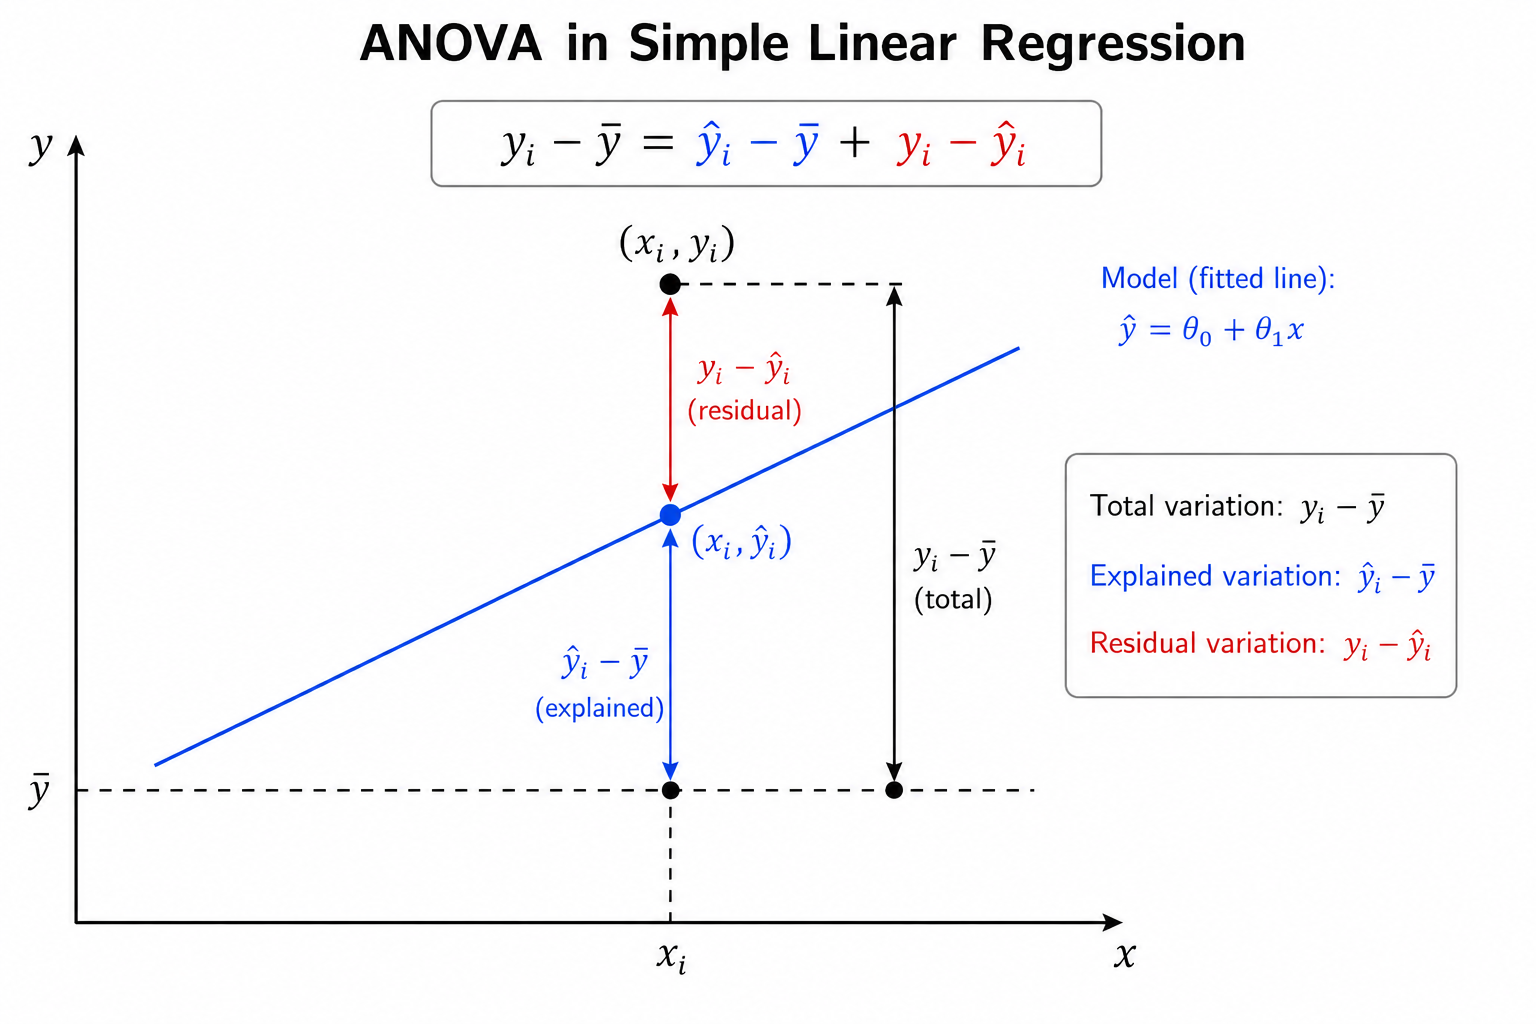
\includegraphics[keepaspectratio]{1-quantitative-finance/figures/anova.png}}

}

\caption{\label{fig-anova}ANOVA decomposition in simple linear
regression}

\end{figure}%

Summing over all observations leads to the classical ANOVA decomposition

\begin{equation}\phantomsection\label{eq-anova-decomposition}{
\mathrm{TSS}
=
\mathrm{MSS}
+
\mathrm{RSS}
}\end{equation}

where

\begin{equation}\phantomsection\label{eq-tss}{
\mathrm{TSS}
=
\sum_{i=1}^{N}
(y_i - \bar{y})^2
}\end{equation}

represents the total variability of the response variable,

\begin{equation}\phantomsection\label{eq-mss}{
\mathrm{MSS}
=
\sum_{i=1}^{N}
(\hat{y}_i - \bar{y})^2
}\end{equation}

corresponds to the variability explained by the regression model, and

\begin{equation}\phantomsection\label{eq-rss-anova}{
\mathrm{RSS}
=
\sum_{i=1}^{N}
(y_i - \hat{y}_i)^2
}\end{equation}

measures the unexplained residual variability.

Dividing each sum of squares by its associated degrees of freedom leads
to the corresponding mean squares. In simple linear regression, the mean
model square and the mean residual square are given by

\begin{equation}\phantomsection\label{eq-mms}{
\mathrm{MMS}
=
\mathrm{MSS}
}\end{equation}

and

\begin{equation}\phantomsection\label{eq-msr}{
\mathrm{MSR}
=
\frac{
\mathrm{RSS}
}{
N - 2
}
}\end{equation}

respectively.

These quantities allow the construction of the F-statistic,

\begin{equation}\phantomsection\label{eq-f-statistic}{
F
=
\frac{
\mathrm{MMS}
}{
\mathrm{MSR}
}
}\end{equation}

which compares the variability explained by the regression model with
the unexplained residual variability. Large values of the F-statistic
suggest that the regression model explains a substantial fraction of the
observed variability relative to the residual noise.

\subsubsection{\texorpdfstring{Coefficient of Determination
(\(R^2\))}{Coefficient of Determination (R\^{}2)}}\label{coefficient-of-determination-r2}

Another commonly used measure in linear regression is the coefficient of
determination, denoted by \(R^2\). This statistic quantifies the
proportion of the total variability in the response variable that is
explained by the regression model.

Using the ANOVA decomposition introduced in
Equation~\ref{eq-anova-decomposition},

\[
\mathrm{TSS}
=
\mathrm{MSS}
+
\mathrm{RSS}
\]

the coefficient of determination can be written as

\begin{equation}\phantomsection\label{eq-r-squared}{
R^2
=
\frac{
\mathrm{MSS}
}{
\mathrm{TSS}
}
=
1
-
\frac{
\mathrm{RSS}
}{
\mathrm{TSS}
}
}\end{equation}

Larger values of \(R^2\) indicate that the model explains a greater
fraction of the observed variability in the data. In particular,
\(R^2 = 1\) corresponds to a perfect fit, whereas \(R^2 = 0\) indicates
that the regression model does not explain the variability of the
response variable better than the sample mean alone.

In the special case of simple linear regression, the coefficient of
determination is directly related to the Pearson correlation coefficient
through

\begin{equation}\phantomsection\label{eq-r-squared-correlation}{
R^2 = r^2
}\end{equation}

where \(r\) denotes the sample correlation between the predictor
variable \(x\) and the response variable \(y\).

Although \(R^2\) provides a useful measure of goodness of fit, a large
value does not necessarily imply that the model is statistically valid
or economically meaningful. For this reason, \(R^2\) is typically
interpreted together with residual diagnostics, hypothesis tests, and
domain-specific considerations.

\subsection{Multiple Linear Regression and the Fama-French
Model}\label{multiple-linear-regression-and-the-fama-french-model}

While the CAPM can be formulated as a simple linear regression model
with a single explanatory factor, the Fama--French three-factor model
extends this framework by incorporating additional sources of systematic
risk. From a statistical perspective, this leads naturally to a multiple
linear regression model in which the response variable depends
simultaneously on several predictors.

For a model with \(M\) explanatory variables, the linear regression
model can be written as

\begin{equation}\phantomsection\label{eq-mlr-scalar}{
y_i
=
\theta_0
+
\theta_1 x_{i1}
+
\theta_2 x_{i2}
+
\cdots
+
\theta_M x_{iM}
+
\varepsilon_i
}\end{equation}

where \(\theta_0\) represents the intercept, \(\theta_1,\dots,\theta_M\)
denote the regression coefficients associated with the predictor
variables, and \(\varepsilon_i\) corresponds to the random error
associated with observation \(i\).

Using matrix notation, the model can be expressed compactly as

\begin{equation}\phantomsection\label{eq-mlr-matrix}{
\mathbf{y}
=
\mathbf{X}
\boldsymbol{\theta}
+
\boldsymbol{\varepsilon}
}\end{equation}

where

\[
\mathbf{y}
=
\begin{bmatrix}
y_1 \\
y_2 \\
\vdots \\
y_N
\end{bmatrix},
\quad
\mathbf{X}
=
\begin{bmatrix}
1 & x_{11} & \cdots & x_{1M} \\
1 & x_{21} & \cdots & x_{2M} \\
\vdots & \vdots & & \vdots \\
1 & x_{N1} & \cdots & x_{NM}
\end{bmatrix}
\]

and

\[
\boldsymbol{\theta}
=
\begin{bmatrix}
\theta_0 \\
\theta_1 \\
\vdots \\
\theta_M
\end{bmatrix},
\quad
\boldsymbol{\varepsilon}
=
\begin{bmatrix}
\varepsilon_1 \\
\varepsilon_2 \\
\vdots \\
\varepsilon_N
\end{bmatrix}
\]

In this representation, the rows of \(\mathbf{X}\) correspond to
observations, while the columns represent the explanatory variables
included in the model. The matrix formulation provides a compact and
computationally efficient framework for parameter estimation and
statistical inference.

Under this interpretation, the Fama--French three-factor model can be
viewed as a particular case of multiple linear regression in which the
excess return of an asset is explained simultaneously by the market
factor, the SMB factor, and the HML factor.

\subsubsection{Ordinary Least Squares
Estimation}\label{ordinary-least-squares-estimation-1}

As in the simple linear regression setting, the parameters of the
multiple linear regression model are estimated by minimizing the
residual sum of squares. Using the matrix formulation introduced in
Equation~\ref{eq-mlr-matrix}, the residual vector can be written as

\begin{equation}\phantomsection\label{eq-mlr-residuals}{
\mathbf{e}
=
\mathbf{y}
-
\mathbf{X}\boldsymbol{\theta}
}\end{equation}

and the corresponding residual sum of squares is given by

\begin{equation}\phantomsection\label{eq-mlr-rss}{
\mathrm{RSS}
=
\mathbf{e}^T\mathbf{e}
=
(\mathbf{y} - \mathbf{X}\boldsymbol{\theta})^T
(\mathbf{y} - \mathbf{X}\boldsymbol{\theta})
}\end{equation}

The ordinary least squares estimator is obtained by minimizing
Equation~\ref{eq-mlr-rss} with respect to the parameter vector
\(\boldsymbol{\theta}\). As in the simple linear regression case, the
optimization problem is convex and admits a unique global minimum
provided that the columns of the design matrix \(\mathbf{X}\) are
linearly independent.

The resulting estimator is given by

\begin{equation}\phantomsection\label{eq-mlr-ols}{
\hat{\boldsymbol{\theta}}
=
(\mathbf{X}^T\mathbf{X})^{-1}
\mathbf{X}^T
\mathbf{y}
}\end{equation}

which generalizes the ordinary least squares estimator introduced
previously for simple linear regression.

The matrix formulation highlights an important aspect of multiple linear
regression: each coefficient measures the linear contribution of its
associated predictor while accounting for the remaining variables
included in the model. In the context of the Fama--French model, this
means that the estimated coefficients associated with the market, SMB,
and HML factors represent their partial contributions to the excess
return of the asset after controlling for the other factors included in
the regression.

\subsubsection{Statistical Interpretation of the
Coefficients}\label{statistical-interpretation-of-the-coefficients}

In multiple linear regression, each regression coefficient measures the
expected variation in the response variable associated with a one-unit
change in the corresponding predictor, while holding the remaining
predictors fixed. This interpretation differs from simple linear
regression, where the effect of the predictor is evaluated without
conditioning on additional explanatory variables.

Under the ordinary least squares framework, the uncertainty associated
with the estimated parameter vector can be characterized through its
covariance matrix, given by

\begin{equation}\phantomsection\label{eq-mlr-covariance}{
\mathrm{Cov}(\hat{\boldsymbol{\theta}})
=
\sigma^2
(\mathbf{X}^T\mathbf{X})^{-1}
}\end{equation}

where \(\sigma^2\) denotes the variance of the random error term.

As in the simple linear regression setting, the variance of the
residuals can be estimated through the residual standard error,

\begin{equation}\phantomsection\label{eq-mlr-rse}{
\mathrm{RSE}
=
\sqrt{
\frac{
\mathrm{RSS}
}{
N - M - 1
}
}
}\end{equation}

where \(N\) represents the number of observations and \(M\) the number
of explanatory variables included in the model.

The diagonal elements of Equation~\ref{eq-mlr-covariance} determine the
standard errors associated with each regression coefficient and provide
a measure of the uncertainty of the parameter estimates. Larger standard
errors indicate greater uncertainty in the estimated contribution of the
corresponding predictor.

In the context of the Fama--French three-factor model, the estimated
coefficients associated with the market, SMB, and HML factors measure
the sensitivity of the asset return to each systematic risk factor after
controlling for the remaining factors included in the regression.
Consequently, the interpretation of each coefficient should always be
understood conditionally on the presence of the other explanatory
variables.

The inclusion of multiple predictors may also introduce statistical
challenges such as multicollinearity, which occurs when explanatory
variables exhibit strong linear dependence. In such cases, coefficient
estimates may become unstable and difficult to interpret, even when the
overall predictive performance of the model remains satisfactory.

\subsubsection{Global Hypothesis Testing and Model
Significance}\label{global-hypothesis-testing-and-model-significance}

In multiple linear regression, it is often important to evaluate whether
the explanatory variables collectively contribute to the model. This can
be assessed through a global hypothesis test of the form

\begin{equation}\phantomsection\label{eq-global-hypothesis}{
\begin{cases}
H_0 :
\theta_1 = \theta_2 = \cdots = \theta_M = 0 \\
H_1 :
\text{at least one } \theta_j \neq 0
\end{cases}
}\end{equation}

Under the null hypothesis, none of the explanatory variables contribute
to explaining the variability of the response variable, implying that
the model does not perform better than using the sample mean alone.

The global significance of the regression model can be evaluated through
the F-statistic,

\begin{equation}\phantomsection\label{eq-global-f-statistic}{
F
=
\frac{
(\mathrm{TSS} - \mathrm{RSS})/M
}{
\mathrm{RSS}/(N - M - 1)
}
}\end{equation}

which compares the variability explained by the model with the
unexplained residual variability after adjusting for the corresponding
degrees of freedom.

Large values of the F-statistic suggest that the explanatory variables
collectively explain a substantial fraction of the observed variability
in the response variable. The corresponding p-value provides a
quantitative measure of the evidence against the null hypothesis.

In the context of the Fama--French three-factor model, the global F-test
evaluates whether the market, SMB, and HML factors jointly contribute to
explaining the excess return of the asset. Consequently, the test
provides a global assessment of the explanatory power of the multifactor
specification relative to a model without risk factors.

\subsubsection{Limitations of Multiple Linear
Regression}\label{limitations-of-multiple-linear-regression}

Although multiple linear regression provides a flexible and
interpretable framework for modeling relationships between variables,
its performance depends on several assumptions and modeling choices. In
practice, violations of these assumptions may affect the reliability of
parameter estimates, confidence intervals, and hypothesis tests.

One important limitation is multicollinearity, which arises when
explanatory variables exhibit strong linear dependence. In such cases,
the regression coefficients may become unstable and highly sensitive to
small changes in the data, making their interpretation more difficult.

Multiple linear regression models may also be affected by omitted
variable bias when relevant explanatory factors are excluded from the
specification. In empirical asset pricing, this issue motivated the
development of multifactor models such as the Fama--French framework,
which extends the CAPM by incorporating additional sources of systematic
risk beyond the market factor alone.

Another practical limitation is that linear regression assumes a linear
relationship between predictors and the response variable. While this
assumption often provides a useful approximation, real financial data
may exhibit nonlinear effects, structural changes, heteroscedasticity,
or temporal dependence that are not fully captured by the model.

Despite these limitations, linear regression models remain fundamental
tools in empirical finance due to their interpretability, computational
efficiency, and strong connection with statistical inference and risk
factor modeling.

\chapter{Unsupervised Learning for Asset
Allocation}\label{unsupervised-learning-for-asset-allocation}

This project explores the use of unsupervised learning techniques for
portfolio construction and risk diversification. The analysis combines
Principal Component Analysis (PCA), hierarchical clustering, and
Hierarchical Risk Parity (HRP) to study how latent market structure and
correlation patterns can be used to build more stable asset allocation
strategies.

Rather than focusing on return forecasting, the project examines how
statistical learning methods can help identify common sources of risk,
reduce redundancy across correlated assets, and improve portfolio
robustness under realistic market conditions. The underlying idea is
that portfolios are often considered diversified based on asset labels,
sectors, or asset classes, even when a small number of common risk
factors continue to drive most of their behaviour. By studying how
assets actually move together, the project aims to construct allocations
that better reflect the underlying structure of market risk.

\section{Problem Definition}\label{problem-definition-1}

Constructing a diversified investment portfolio is one of the central
problems in quantitative finance. In practice, investors must allocate
capital across a large universe of financial instruments while balancing
expected returns, risk exposure, diversification, and portfolio
stability. Although the classical mean--variance framework introduced by
Harry Markowitz remains foundational in modern portfolio theory, its
practical implementation presents important limitations when applied to
real financial markets.

Traditional portfolio optimization methods rely heavily on the
estimation and inversion of covariance matrices. In large and highly
correlated markets, these matrices often become numerically unstable and
highly sensitive to small estimation errors. As a result, optimized
portfolios may exhibit unintuitive allocations, excessive concentration,
poor robustness, and unstable out-of-sample performance. This issue
becomes more severe as the number of assets increases and correlation
structures evolve through time.

At the same time, financial markets naturally exhibit latent and
hierarchical structures that are not fully captured by traditional
optimization approaches. Assets rarely behave as isolated entities.
Instead, they tend to move collectively according to sector dynamics,
macroeconomic conditions, liquidity regimes, or broader market factors.
Under stressed market conditions, assets that appear diversified on
paper may suddenly behave in remarkably similar ways, reducing
diversification precisely when it becomes most important.

The motivation behind this project is to explore whether unsupervised
learning techniques can provide a more robust and structurally stable
framework for asset allocation. Rather than treating portfolio
construction purely as a constrained optimization problem, the project
approaches it as a problem of identifying and organizing the underlying
geometry of market risk.

To address this, the analysis combines two complementary perspectives.
First, Principal Component Analysis (PCA) is used to study the dominant
sources of variation in the market and to represent the covariance
structure in terms of orthogonal risk components. This provides a
compact representation of the market structure while reducing redundancy
across highly correlated assets. Second, hierarchical clustering
techniques are used to identify groups of statistically similar assets
and to construct portfolios using Hierarchical Risk Parity (HRP), a
methodology designed to improve allocation stability without requiring
direct inversion of the covariance matrix.

The objective is not simply to maximize historical returns, but to
investigate whether combining spectral methods and hierarchical
structures can produce portfolios that are more diversified,
interpretable, and robust under changing market conditions. The project
therefore sits at the intersection of quantitative finance, machine
learning, and statistical risk modeling, with a strong emphasis on
practical portfolio construction rather than purely theoretical
optimization.

\section{Modeling Approach}\label{modeling-approach-1}

The modeling approach adopted in this project treats portfolio
construction as a problem of understanding the structure of market risk.
The analysis focuses on how assets move together, how risk concentrates
across the market, and how correlation patterns affect diversification
under changing market conditions.

Financial markets are rarely composed of independent assets. Securities
that belong to different sectors or asset classes often remain exposed
to the same underlying drivers, particularly during periods of stress
when correlations tend to increase. This means that portfolios that
appear diversified on paper may still contain significant hidden
concentrations of risk.

The analysis begins with Principal Component Analysis (PCA), following
the general perspective of statistical risk decomposition discussed in
\citeproc{ref-meucci2005risk}{{[}11{]}} and the idea of principal
portfolios introduced in \citeproc{ref-partovi2004principal}{{[}12{]}}.
PCA is used to study the covariance structure of the market and identify
the dominant directions of variation across asset returns. In practice,
a relatively small number of components often explains a large
proportion of total market variance, suggesting that many assets
continue to react to common underlying factors even when they appear
superficially diversified.

The covariance matrix is decomposed according to

\begin{equation}\phantomsection\label{eq-spectral-decomposition}{
\Sigma = Q \Lambda Q^\top
}\end{equation}

where \(Q\) contains the eigenvectors and \(\Lambda\) the associated
eigenvalues. The eigenvectors define orthogonal directions in the
transformed risk space, while the eigenvalues measure the variance
explained by each component. This decomposition provides a compact
representation of the market structure and helps distinguish between
broad market behaviour and more localized sources of variation.

The PCA transformation can also be interpreted as a rotation of the
original return space into an orthogonal basis of uncorrelated
components,

\begin{equation}\phantomsection\label{eq-pca-rotation}{
\tilde{\mathbf{R}} = \Gamma^\top \mathbf{R}
}\end{equation}

where \(\mathbf{R}\) denotes the original return vector and
\(\tilde{\mathbf{R}}\) its representation in the transformed PCA space.
Portfolio returns preserve their underlying structure under this
transformation while becoming easier to interpret in terms of
independent sources of market variation.

PCA is used as a diagnostic tool for studying market structure before
constructing the final allocation. The portfolio construction stage is
based on Hierarchical Risk Parity (HRP), introduced in
\citeproc{ref-lopez2016building}{{[}13{]}} and further developed in
\citeproc{ref-de2018advances}{{[}14{]}}. Unlike traditional
mean--variance optimization frameworks, HRP does not require direct
inversion of the covariance matrix, avoiding part of the numerical
instability associated with highly correlated asset universes and
estimation error.

The clustering stage identifies groups of statistically similar assets
using a correlation-based distance measure,

\begin{equation}\phantomsection\label{eq-correlation-distance}{
d_{ij} = \sqrt{\frac{1}{2}(1 - \rho_{ij})}
}\end{equation}

where \(\rho_{ij}\) denotes the correlation between assets \(i\) and
\(j\). Assets with similar behaviour are grouped together into a
hierarchical structure that reflects the organization of the market more
naturally than a flat covariance matrix alone.

Portfolio weights are then allocated recursively across the hierarchy,
reducing concentration in highly correlated regions of the market. In
practice, this tends to produce more stable allocations than traditional
mean--variance optimization procedures, where small changes in
covariance estimates can generate disproportionately large changes in
portfolio weights.

An equally weighted \(1/N\) portfolio is used as a benchmark throughout
the analysis. Although simple, this benchmark provides an important
reference point when evaluating whether additional model complexity
leads to meaningful improvements in diversification and portfolio
robustness out-of-sample.

The resulting framework combines spectral analysis, clustering
techniques, and hierarchical risk allocation to study diversification
from a structural perspective, with emphasis on robustness and stability
under changing market conditions.

\section{Methodology and
Implementation}\label{methodology-and-implementation-1}

The empirical analysis was conducted using a diversified universe of
U.S. equities representing multiple sectors of the economy, including
technology, financials, energy, healthcare, consumer staples,
communication services, and retail. The selected assets were chosen to
provide exposure to different market dynamics while still allowing
meaningful correlation structures and latent factor relationships to
emerge throughout the analysis.

The asset universe used in the study is summarized in
Table~\ref{tbl-asset-universe}.

\begin{longtable}[]{@{}cc@{}}
\caption{Selected asset universe used throughout the portfolio
construction and clustering experiments.
}\label{tbl-asset-universe}\tabularnewline
\toprule\noalign{}
Ticker & Sector \\
\midrule\noalign{}
\endfirsthead
\toprule\noalign{}
Ticker & Sector \\
\midrule\noalign{}
\endhead
\bottomrule\noalign{}
\endlastfoot
AAPL & Technology \\
MSFT & Technology \\
GOOGL & Communication Services \\
AMZN & Consumer Discretionary \\
META & Communication Services \\
JPM & Financials \\
BAC & Financials \\
XOM & Energy \\
CVX & Energy \\
JNJ & Healthcare \\
PFE & Healthcare \\
PG & Consumer Staples \\
KO & Consumer Staples \\
WMT & Retail \\
HD & Consumer Discretionary \\
\end{longtable}

Daily adjusted closing prices were collected and transformed into
continuously compounded daily returns. The analysis focused primarily on
the covariance and correlation structure of returns rather than on
absolute price levels. Figure~\ref{fig-adjusted-closing-prices} presents
the evolution of adjusted prices across the selected assets during the
evaluation period.

\begin{figure}

\centering{

\pandocbounded{
\includegraphics[keepaspectratio]{1-quantitative-finance/../notebooks-and-scripts/1-quantitative-finance/2-unsupervised-learning-for-asset-allocation/r/1-unsupervised-learning-for-asset-allocation-figures/closing-prices.png}}

}

\caption{\label{fig-adjusted-closing-prices}Adjusted closing prices of
the selected assets over the analysis period, illustrating heterogeneous
price dynamics and sector-specific trends across the asset universe.}

\end{figure}%

Although the selected securities belong to different sectors, the return
series exhibit periods of synchronized behaviour, particularly during
episodes of elevated market stress. This becomes more evident when
examining the daily return dynamics shown in
Figure~\ref{fig-daily-returns}.

\begin{figure}

\centering{

\pandocbounded{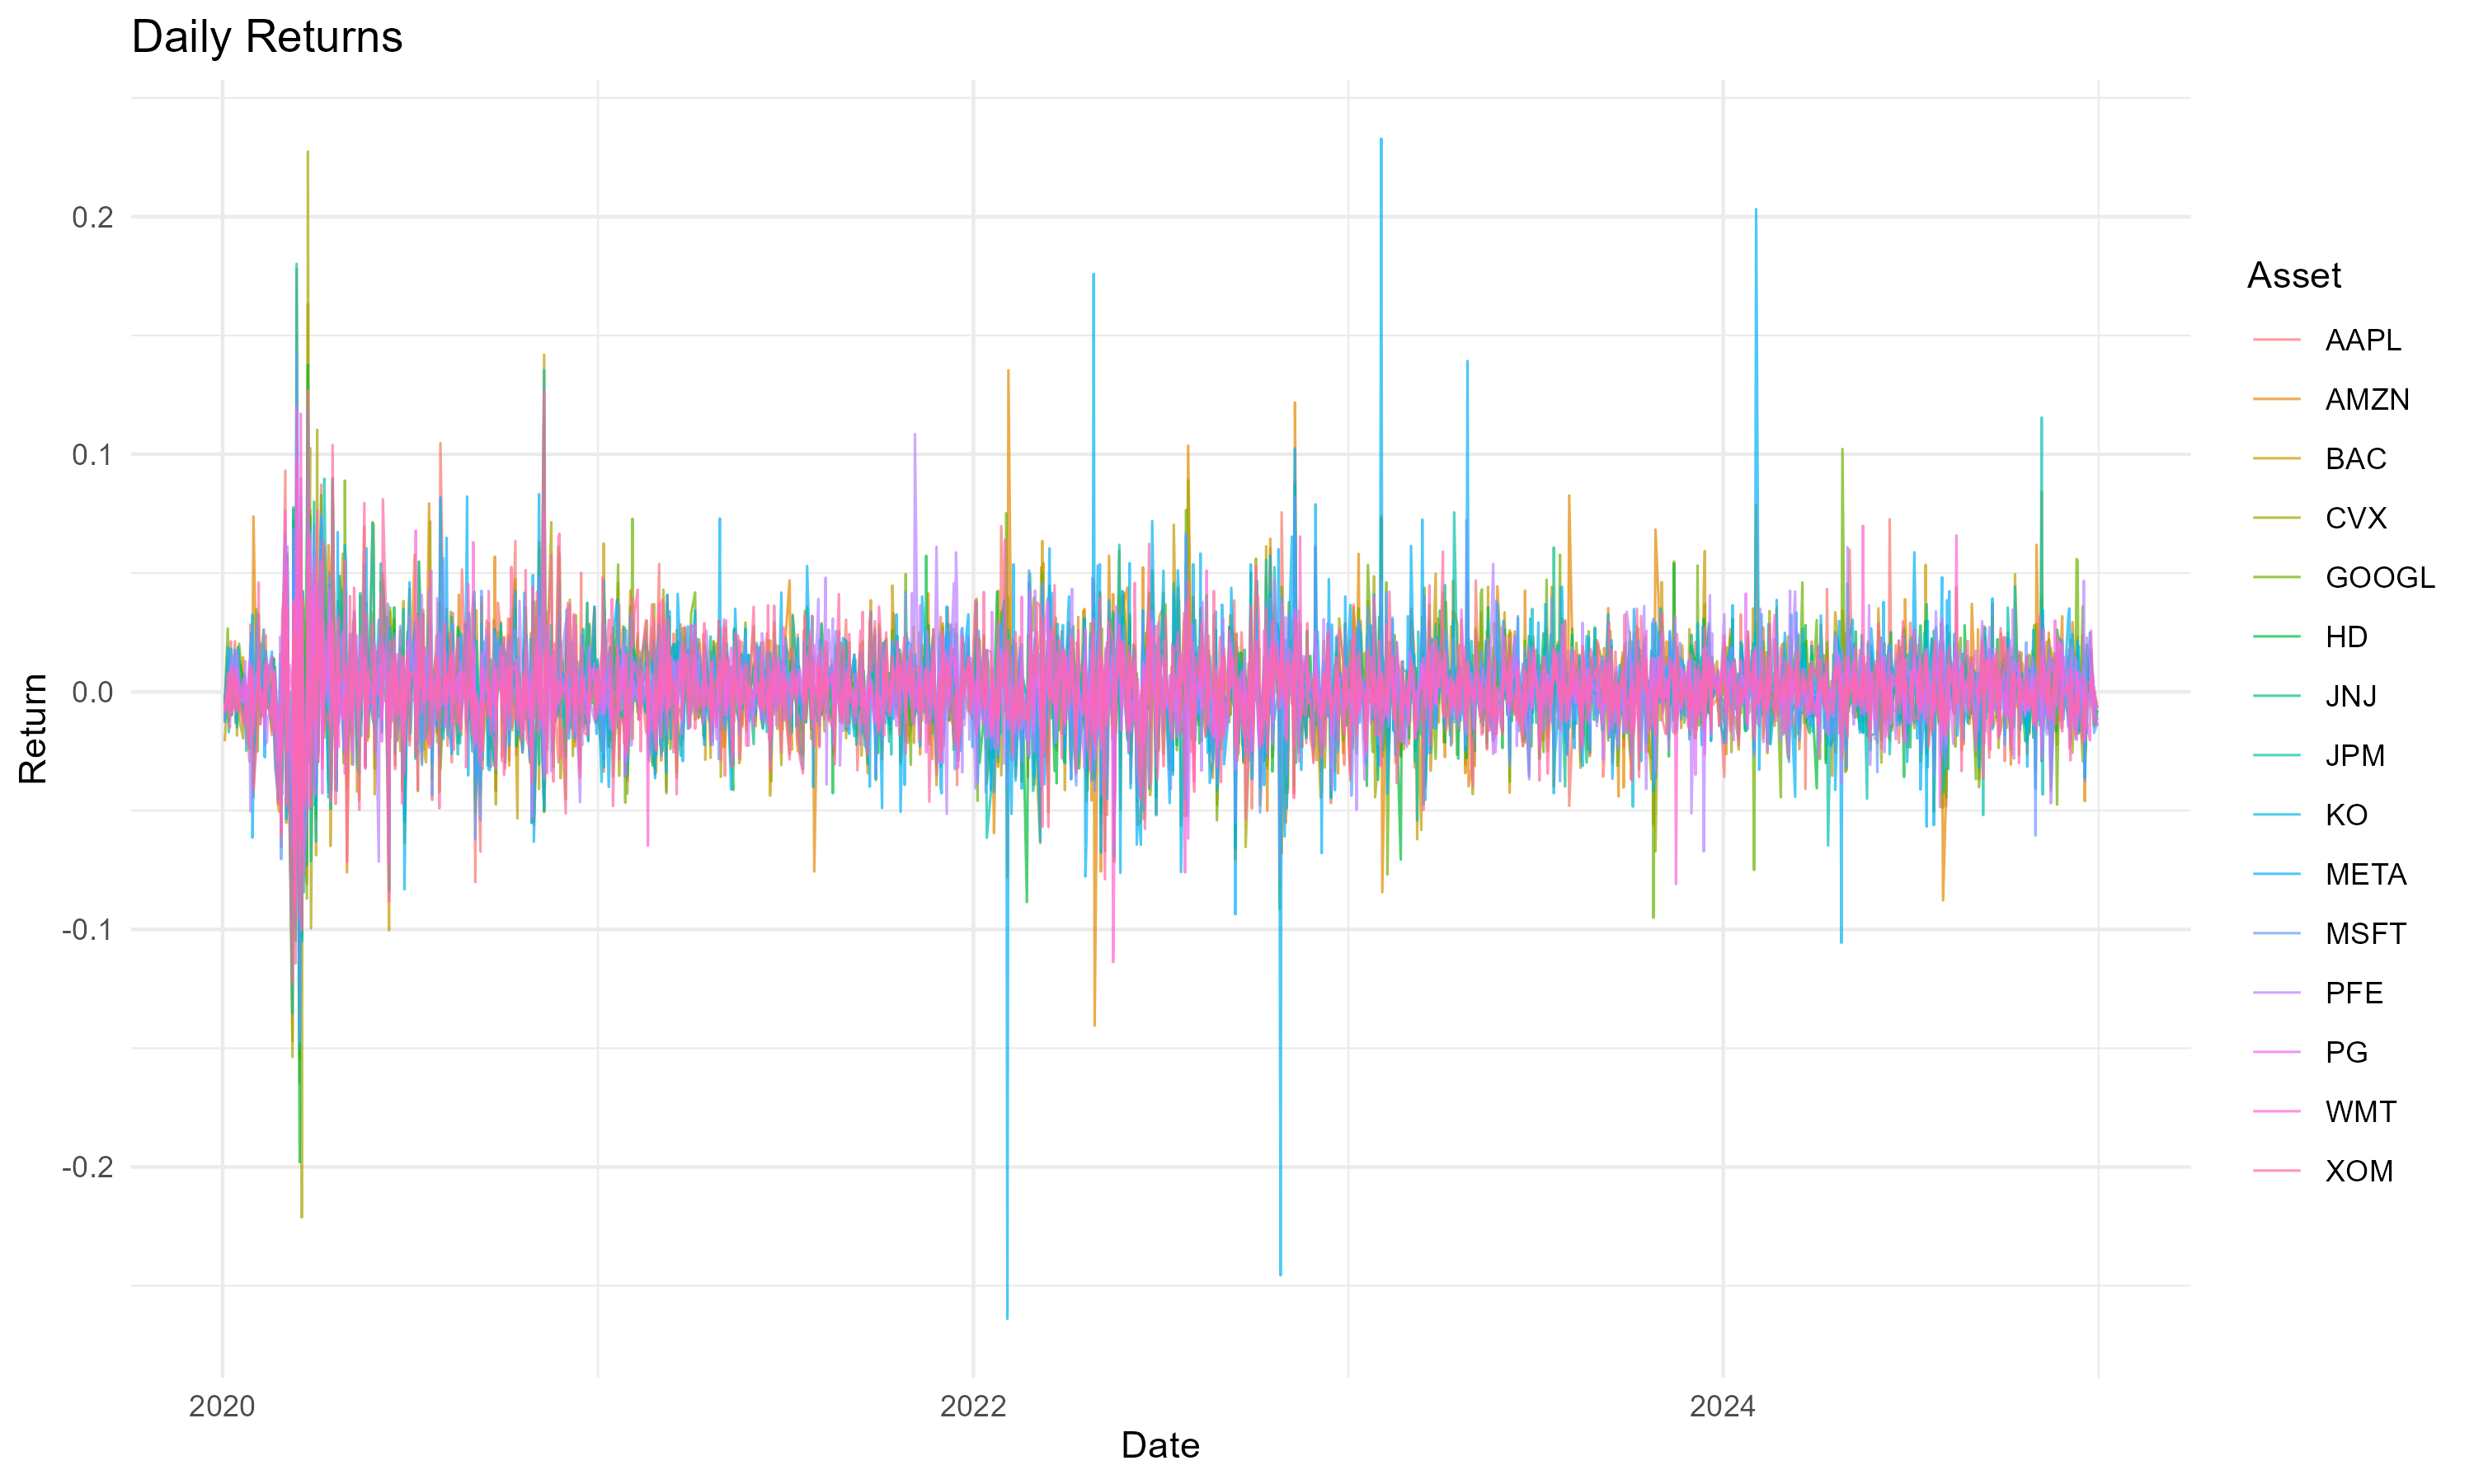
\includegraphics[keepaspectratio]{1-quantitative-finance/../notebooks-and-scripts/1-quantitative-finance/2-unsupervised-learning-for-asset-allocation/r/1-unsupervised-learning-for-asset-allocation-figures/daily-returns.png}}

}

\caption{\label{fig-daily-returns}Daily returns of the selected assets
over the analysis period, highlighting volatility clustering and
heterogeneous risk dynamics across the asset universe.}

\end{figure}%

The return series display the volatility clustering commonly observed in
financial markets, together with periods of sharply increasing
cross-asset dependence. The volatility spikes and correlation increases
visible in the data are precisely the conditions under which naïve
diversification can become less effective, providing the empirical
motivation for the PCA and HRP framework adopted in this study.

The covariance matrix shown in Figure~\ref{fig-covariance-matrix} was
estimated directly from the daily return series and used throughout the
PCA and HRP stages of the analysis.

\begin{figure}

\centering{

\pandocbounded{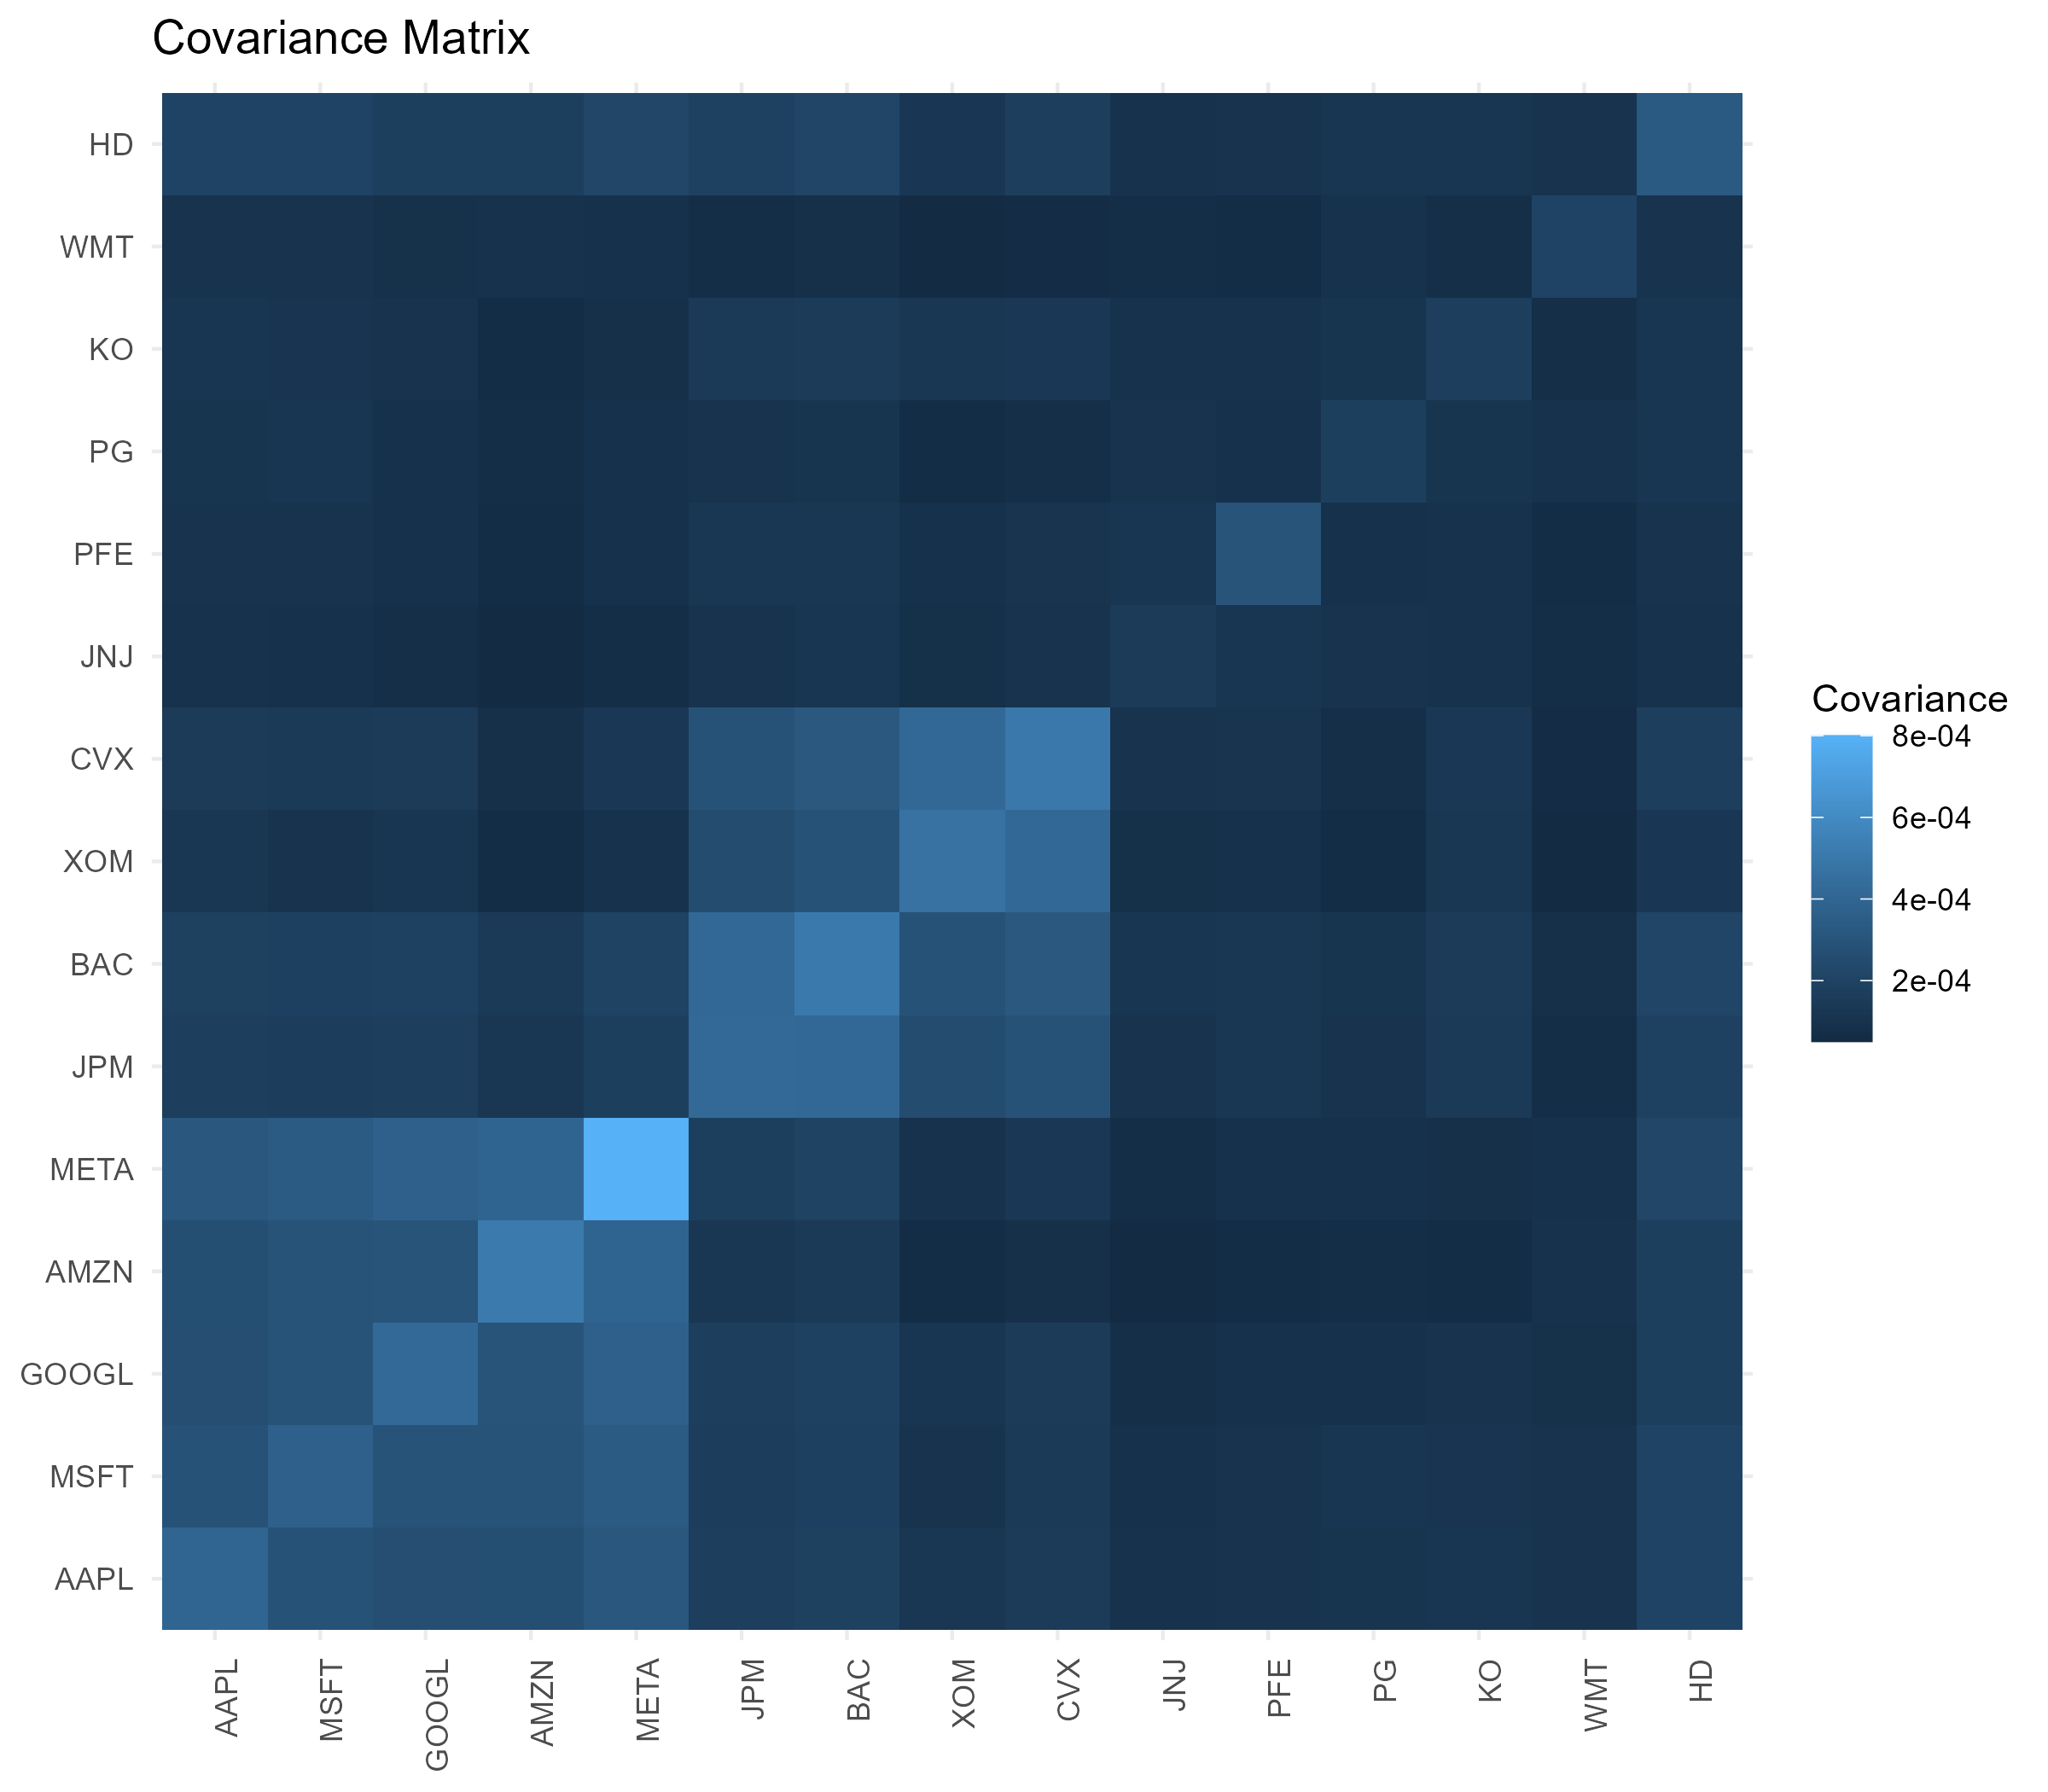
\includegraphics[keepaspectratio]{1-quantitative-finance/../notebooks-and-scripts/1-quantitative-finance/2-unsupervised-learning-for-asset-allocation/r/1-unsupervised-learning-for-asset-allocation-figures/covariance-matrix.png}}

}

\caption{\label{fig-covariance-matrix}Covariance matrix of asset
returns, showing the magnitude of joint variability across the selected
assets used in portfolio risk estimation and allocation.}

\end{figure}%

The corresponding correlation matrix is presented in
Figure~\ref{fig-correlation-matrix}. Several economically meaningful
relationships already become visible at this stage, particularly among
technology, financial, energy, healthcare, and consumer staples stocks.

\begin{figure}

\centering{

\pandocbounded{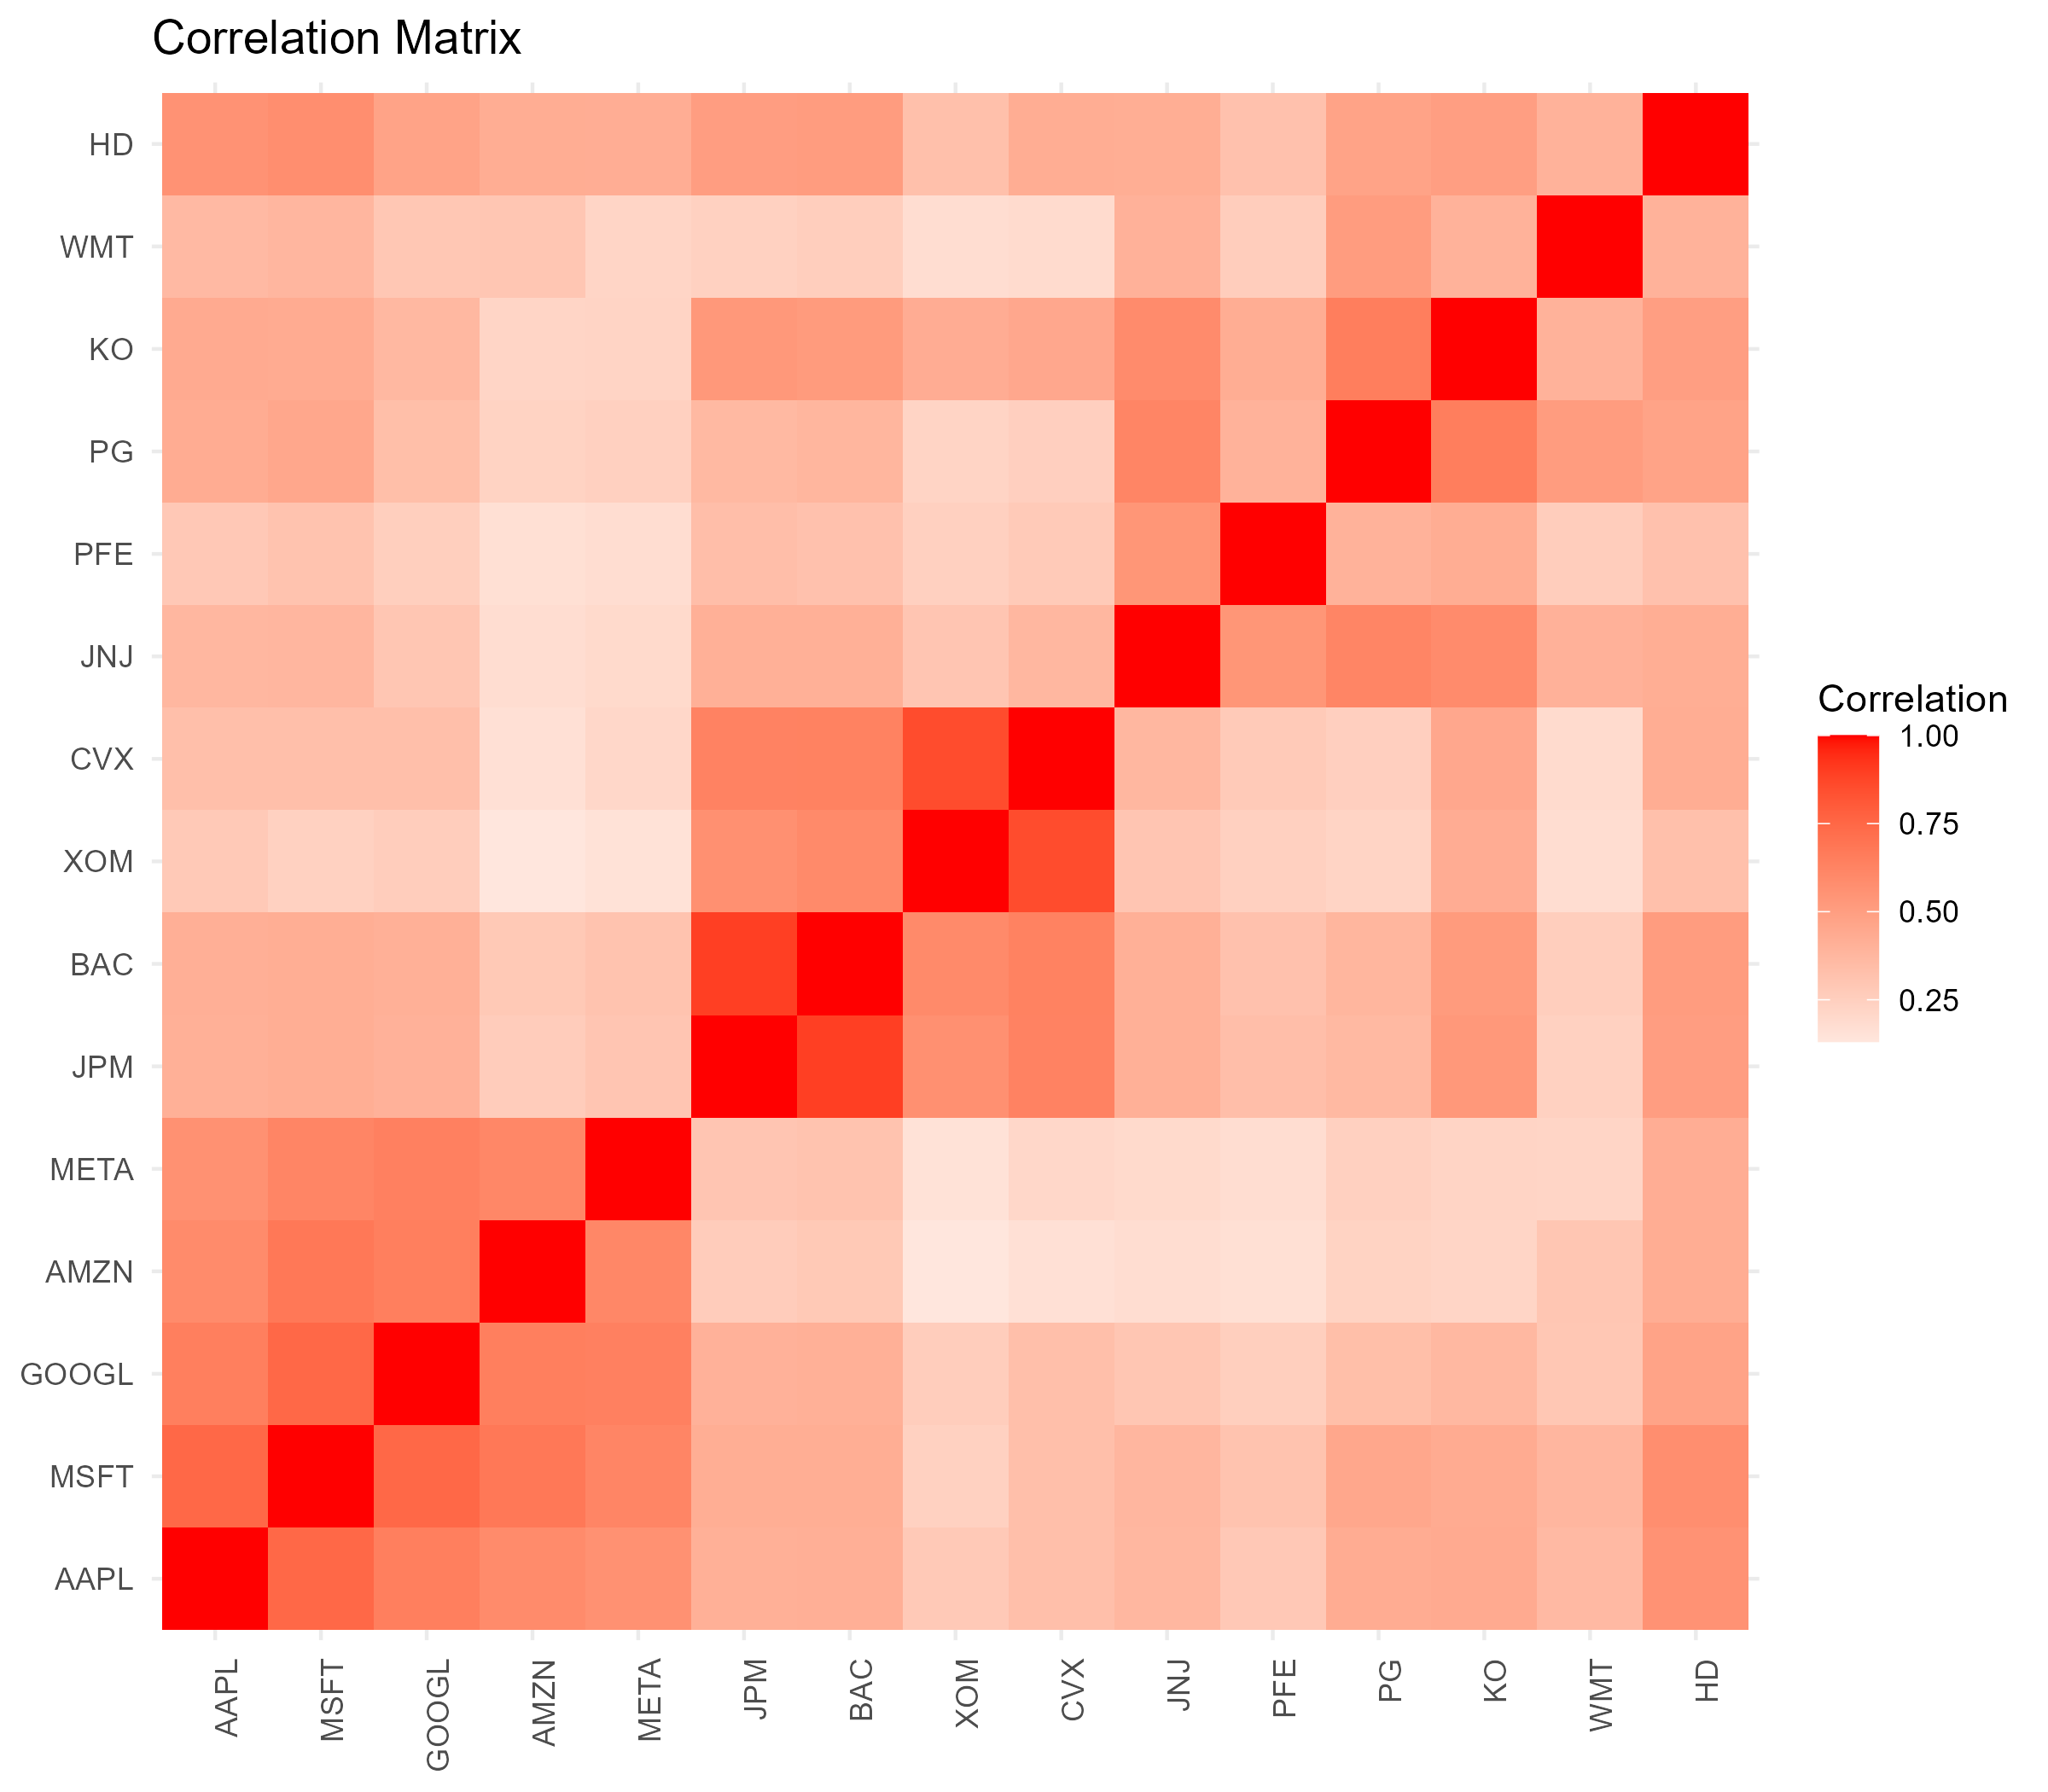
\includegraphics[keepaspectratio]{1-quantitative-finance/../notebooks-and-scripts/1-quantitative-finance/2-unsupervised-learning-for-asset-allocation/r/1-unsupervised-learning-for-asset-allocation-figures/correlation-matrix.png}}

}

\caption{\label{fig-correlation-matrix}Correlation matrix of asset
returns, showing the dependence structure across the selected assets
prior to hierarchical clustering reordering.}

\end{figure}%

Principal Component Analysis (PCA) was then applied to study the latent
structure of market risk. The decomposition was performed on the
covariance matrix of returns, allowing the market structure to be
represented in terms of orthogonal components ranked by explained
variance.

The explained variance associated with each principal component is
summarized in Table~\ref{tbl-pca-explained-variance}.

\begin{longtable}[]{@{}ccc@{}}
\caption{Explained and cumulative variance ratios obtained from
Principal Component Analysis (PCA) applied to asset returns.
}\label{tbl-pca-explained-variance}\tabularnewline
\toprule\noalign{}
Component & Explained Variance & Cumulative Variance \\
\midrule\noalign{}
\endfirsthead
\toprule\noalign{}
Component & Explained Variance & Cumulative Variance \\
\midrule\noalign{}
\endhead
\bottomrule\noalign{}
\endlastfoot
PC1 & 0.4638 & 0.4638 \\
PC2 & 0.1793 & 0.6431 \\
PC3 & 0.0740 & 0.7170 \\
PC4 & 0.0512 & 0.7682 \\
PC5 & 0.0466 & 0.8148 \\
PC6 & 0.0352 & 0.8500 \\
PC7 & 0.0297 & 0.8798 \\
PC8 & 0.0262 & 0.9060 \\
PC9 & 0.0230 & 0.9289 \\
PC10 & 0.0181 & 0.9470 \\
PC11 & 0.0144 & 0.9614 \\
PC12 & 0.0123 & 0.9737 \\
PC13 & 0.0102 & 0.9839 \\
PC14 & 0.0084 & 0.9923 \\
PC15 & 0.0077 & 1.0000 \\
\end{longtable}

The first principal component explains approximately 46\% of total
variance, while the first two components together account for roughly
64\%. The first five components explain more than 80\% of total
variance, indicating that a relatively small number of latent factors
captures much of the variability in the asset universe.
Figure~\ref{fig-explained-variance-ratio} and
Figure~\ref{fig-cumulative-explained-variance} illustrate this
concentration of variance visually.

\begin{figure}

\centering{

\pandocbounded{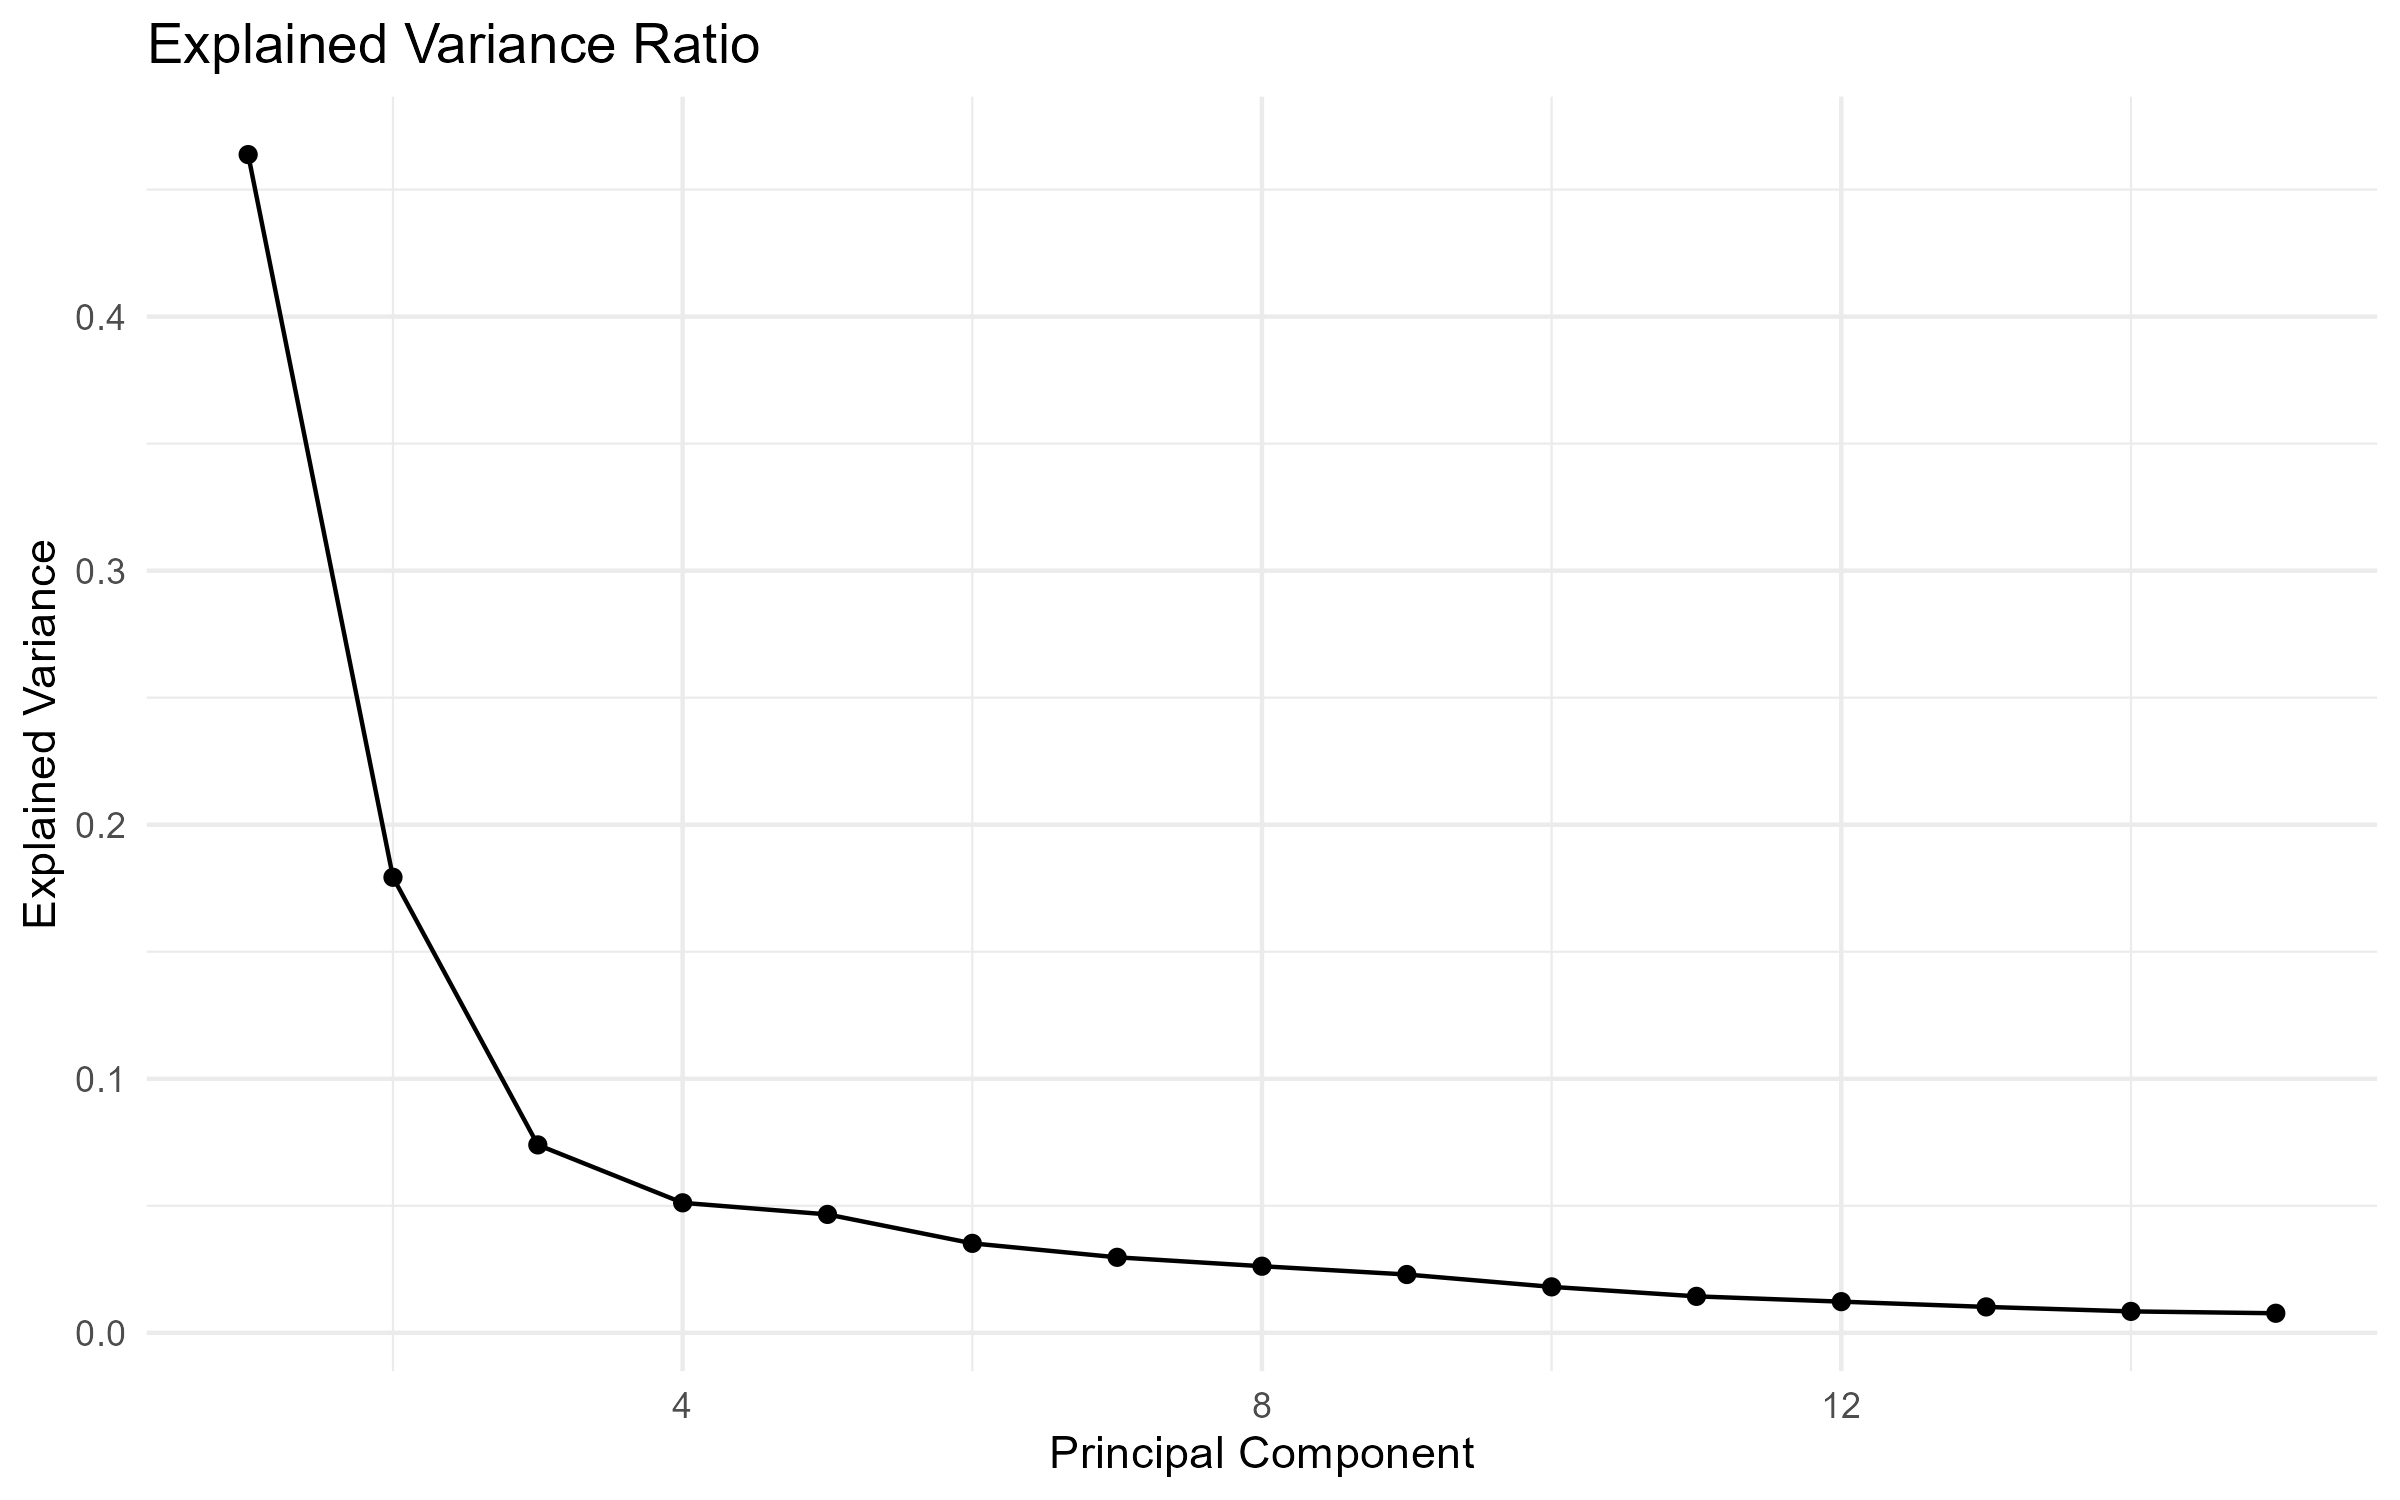
\includegraphics[keepaspectratio]{1-quantitative-finance/../notebooks-and-scripts/1-quantitative-finance/2-unsupervised-learning-for-asset-allocation/r/1-unsupervised-learning-for-asset-allocation-figures/explained-variance-ratio.png}}

}

\caption{\label{fig-explained-variance-ratio}Explained variance ratio
for each principal component obtained from PCA, showing that the first
components capture most of the variability in the asset return space.}

\end{figure}%

\begin{figure}

\centering{

\pandocbounded{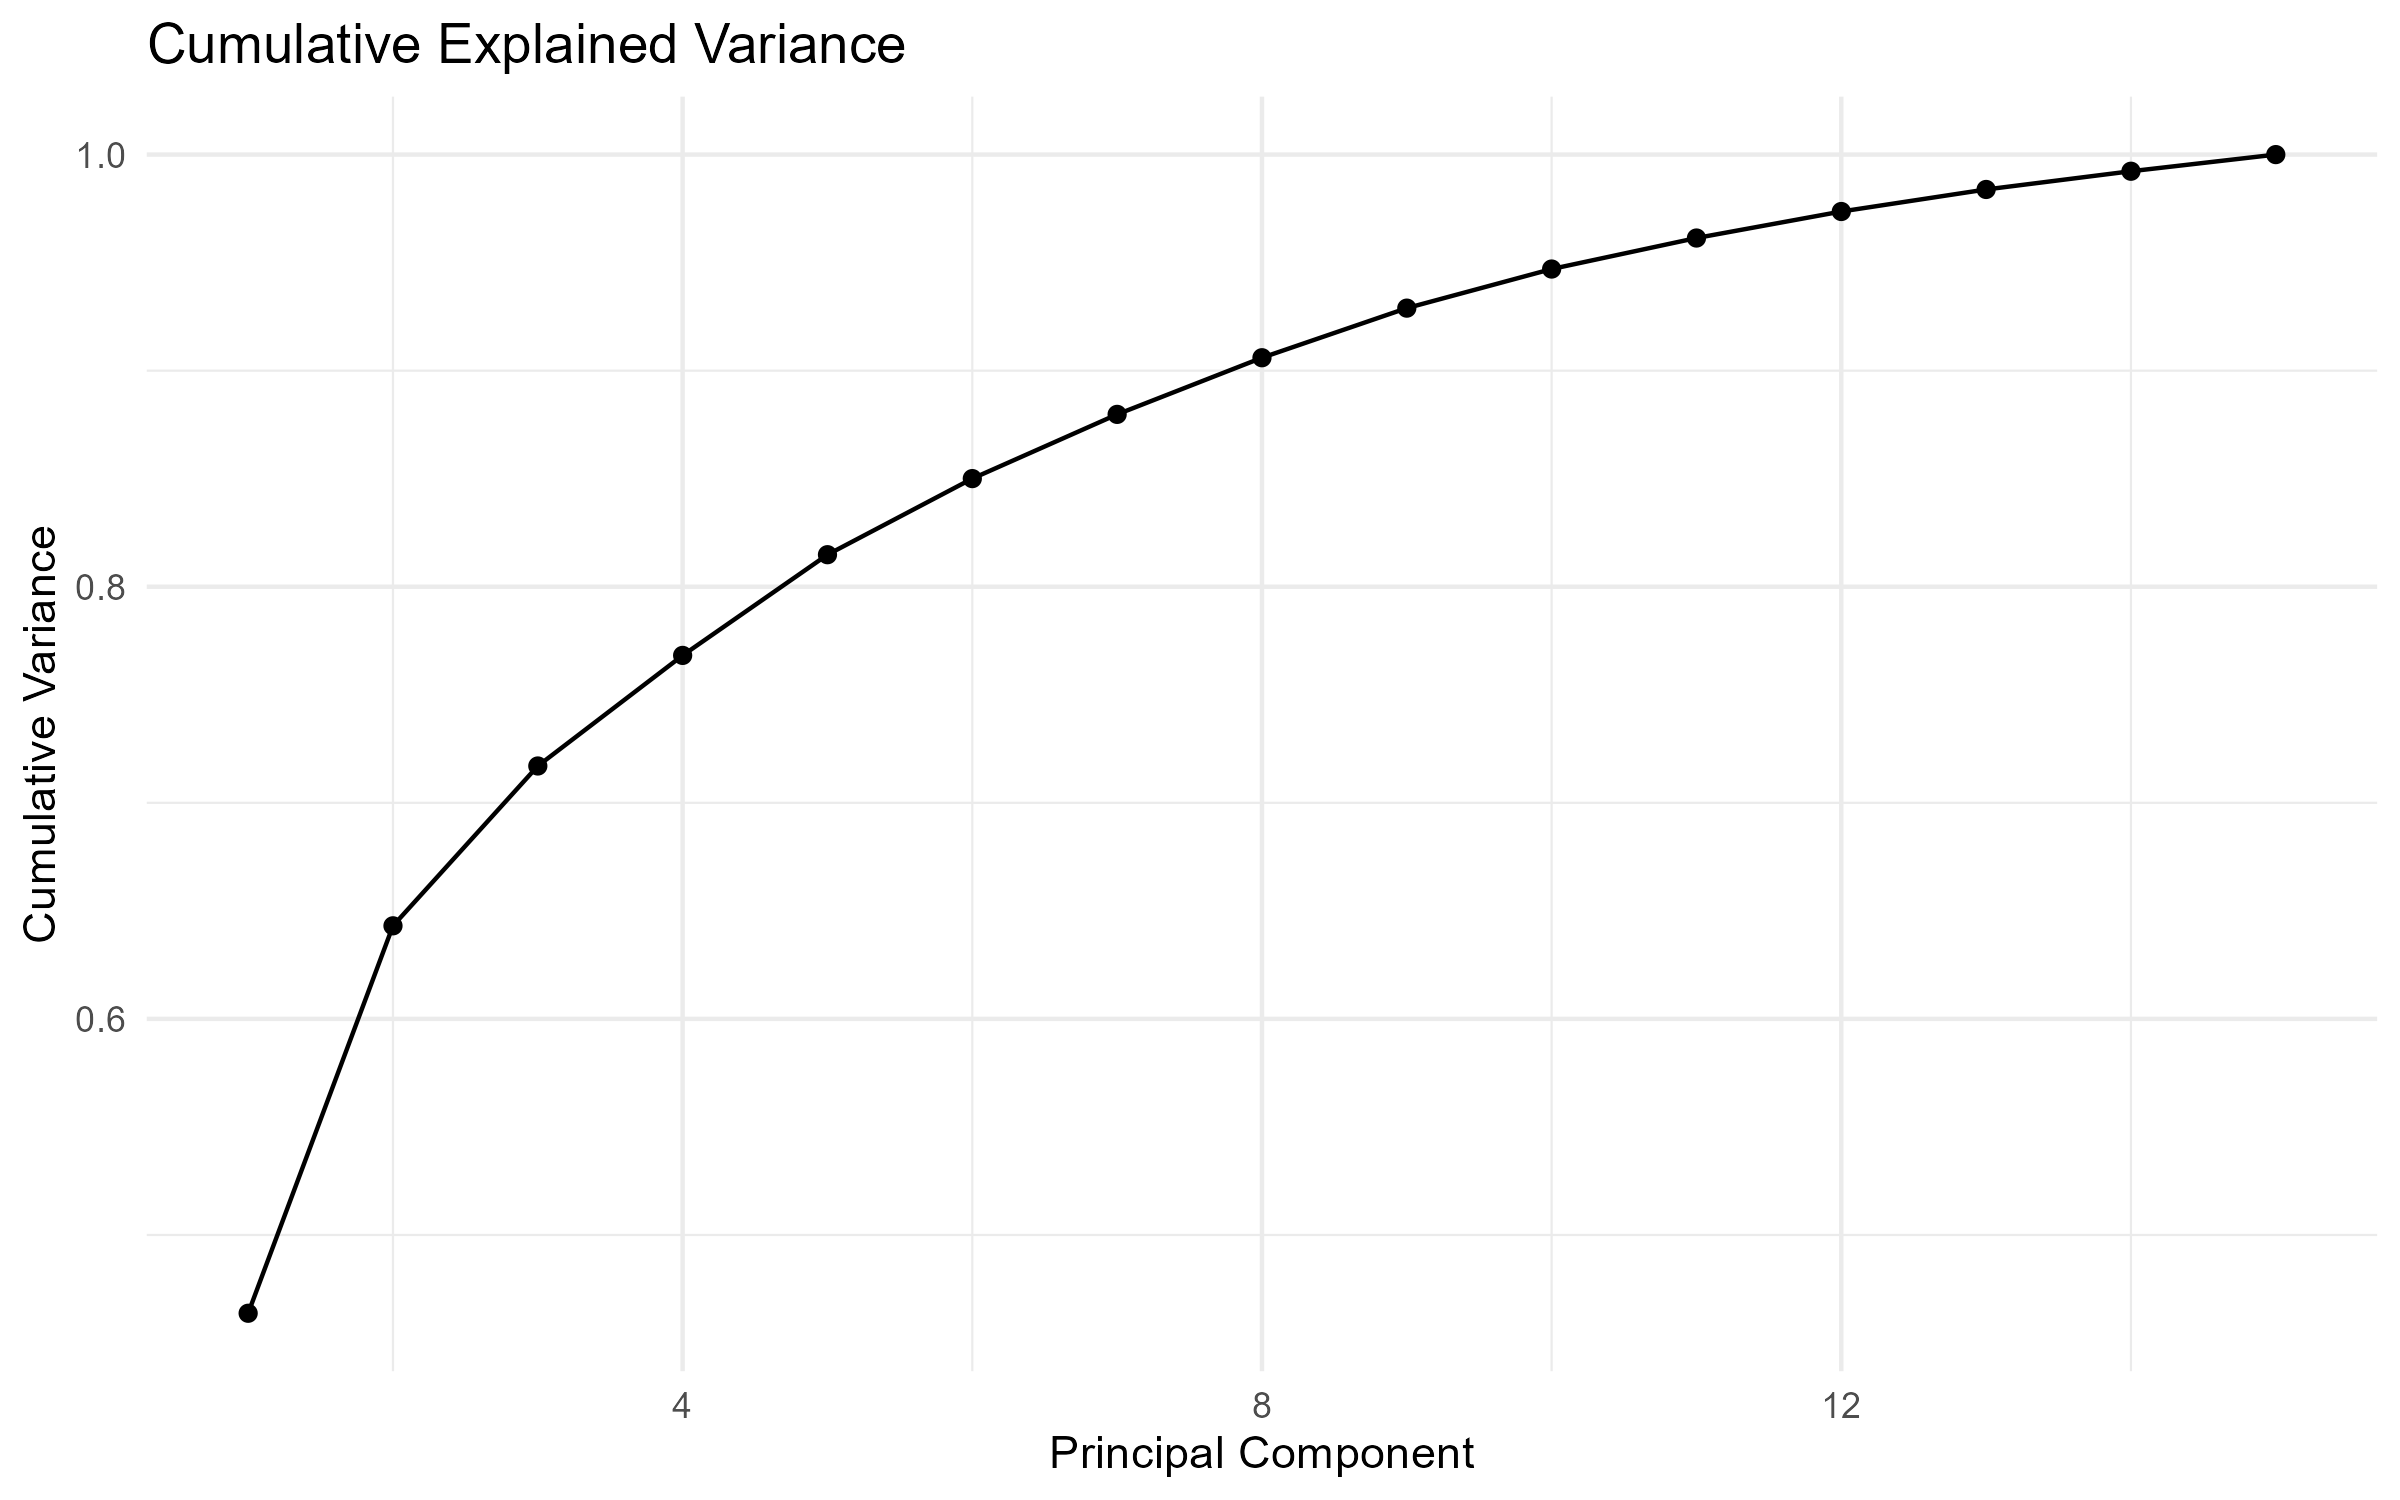
\includegraphics[keepaspectratio]{1-quantitative-finance/../notebooks-and-scripts/1-quantitative-finance/2-unsupervised-learning-for-asset-allocation/r/1-unsupervised-learning-for-asset-allocation-figures/cumulative-explained-variance.png}}

}

\caption{\label{fig-cumulative-explained-variance}Cumulative explained
variance obtained from Principal Component Analysis (PCA), showing how
the first principal components capture most of the variability in the
asset return space.}

\end{figure}%

The first principal component captures a broad market-related factor
affecting most assets simultaneously, consistent with its dominant
contribution to total variance. Subsequent components explain
progressively smaller fractions of variance and reveal more localized
sectoral structures that are less visible in the original return space.

\begin{figure}

\centering{

\pandocbounded{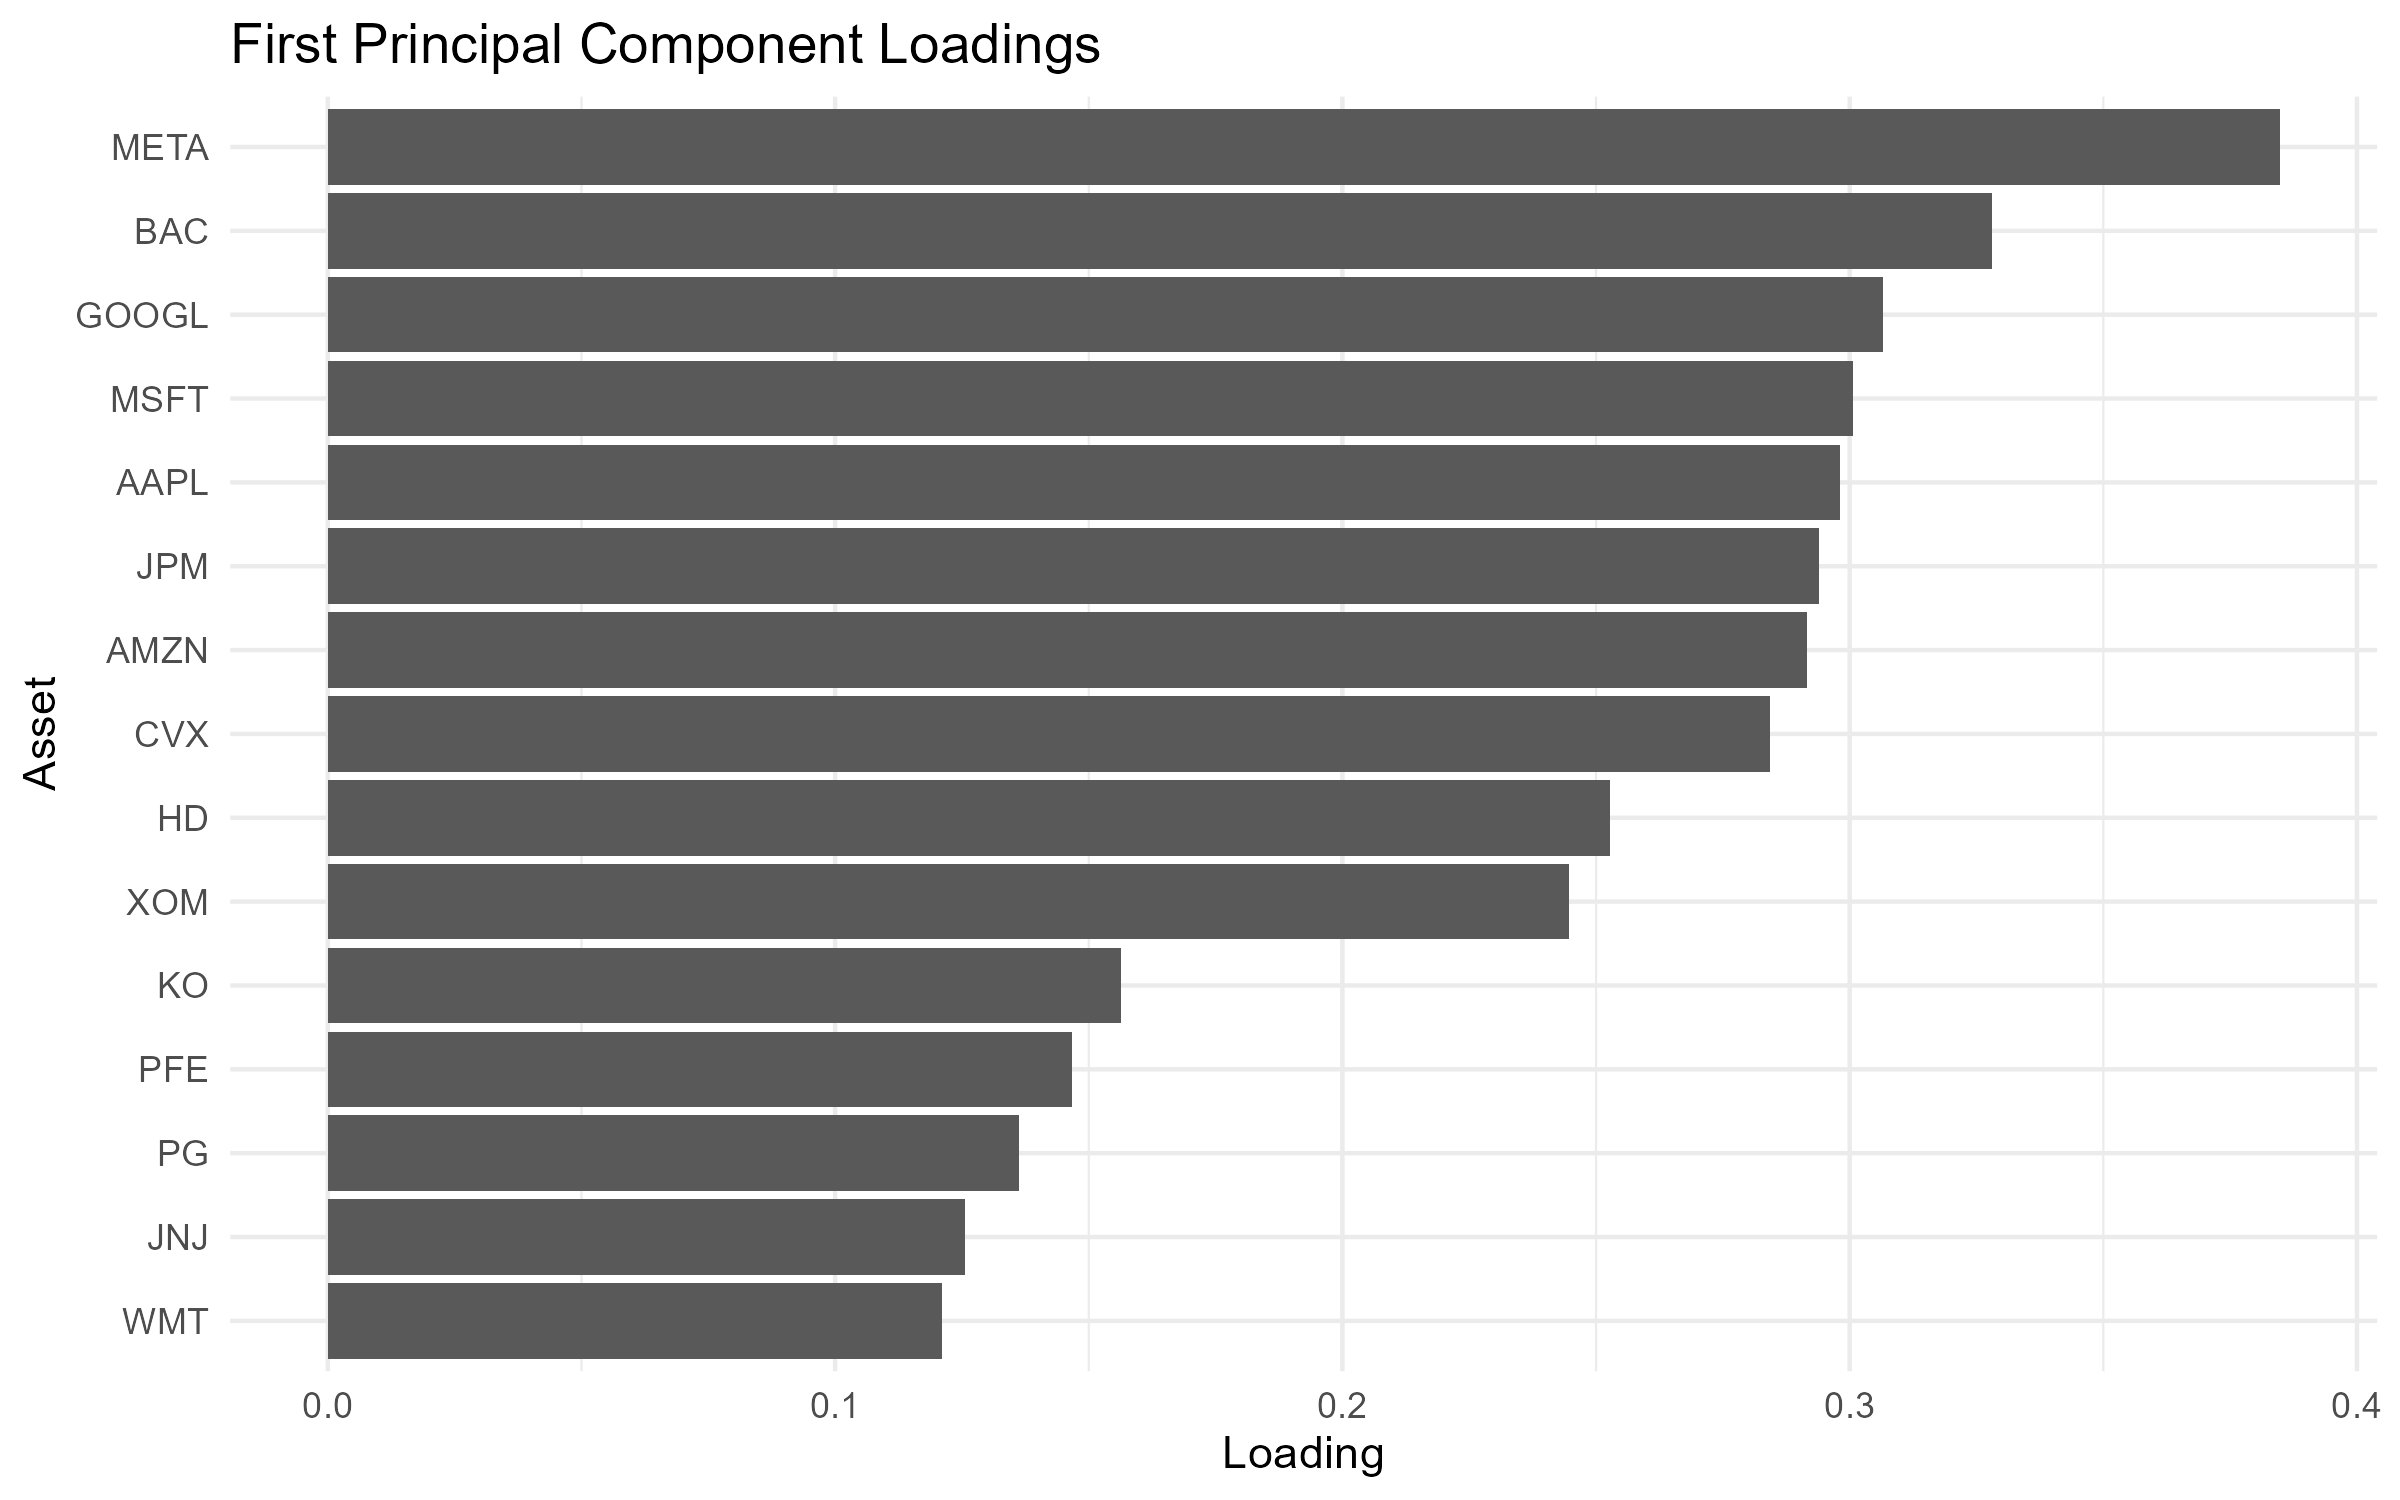
\includegraphics[keepaspectratio]{1-quantitative-finance/../notebooks-and-scripts/1-quantitative-finance/2-unsupervised-learning-for-asset-allocation/r/1-unsupervised-learning-for-asset-allocation-figures/pc1-loadings.png}}

}

\caption{\label{fig-pc1-loadings}Loadings of the first principal
component obtained from PCA, illustrating the assets that contribute
most strongly to the dominant common risk factor in the portfolio
universe.}

\end{figure}%

\begin{figure}

\centering{

\pandocbounded{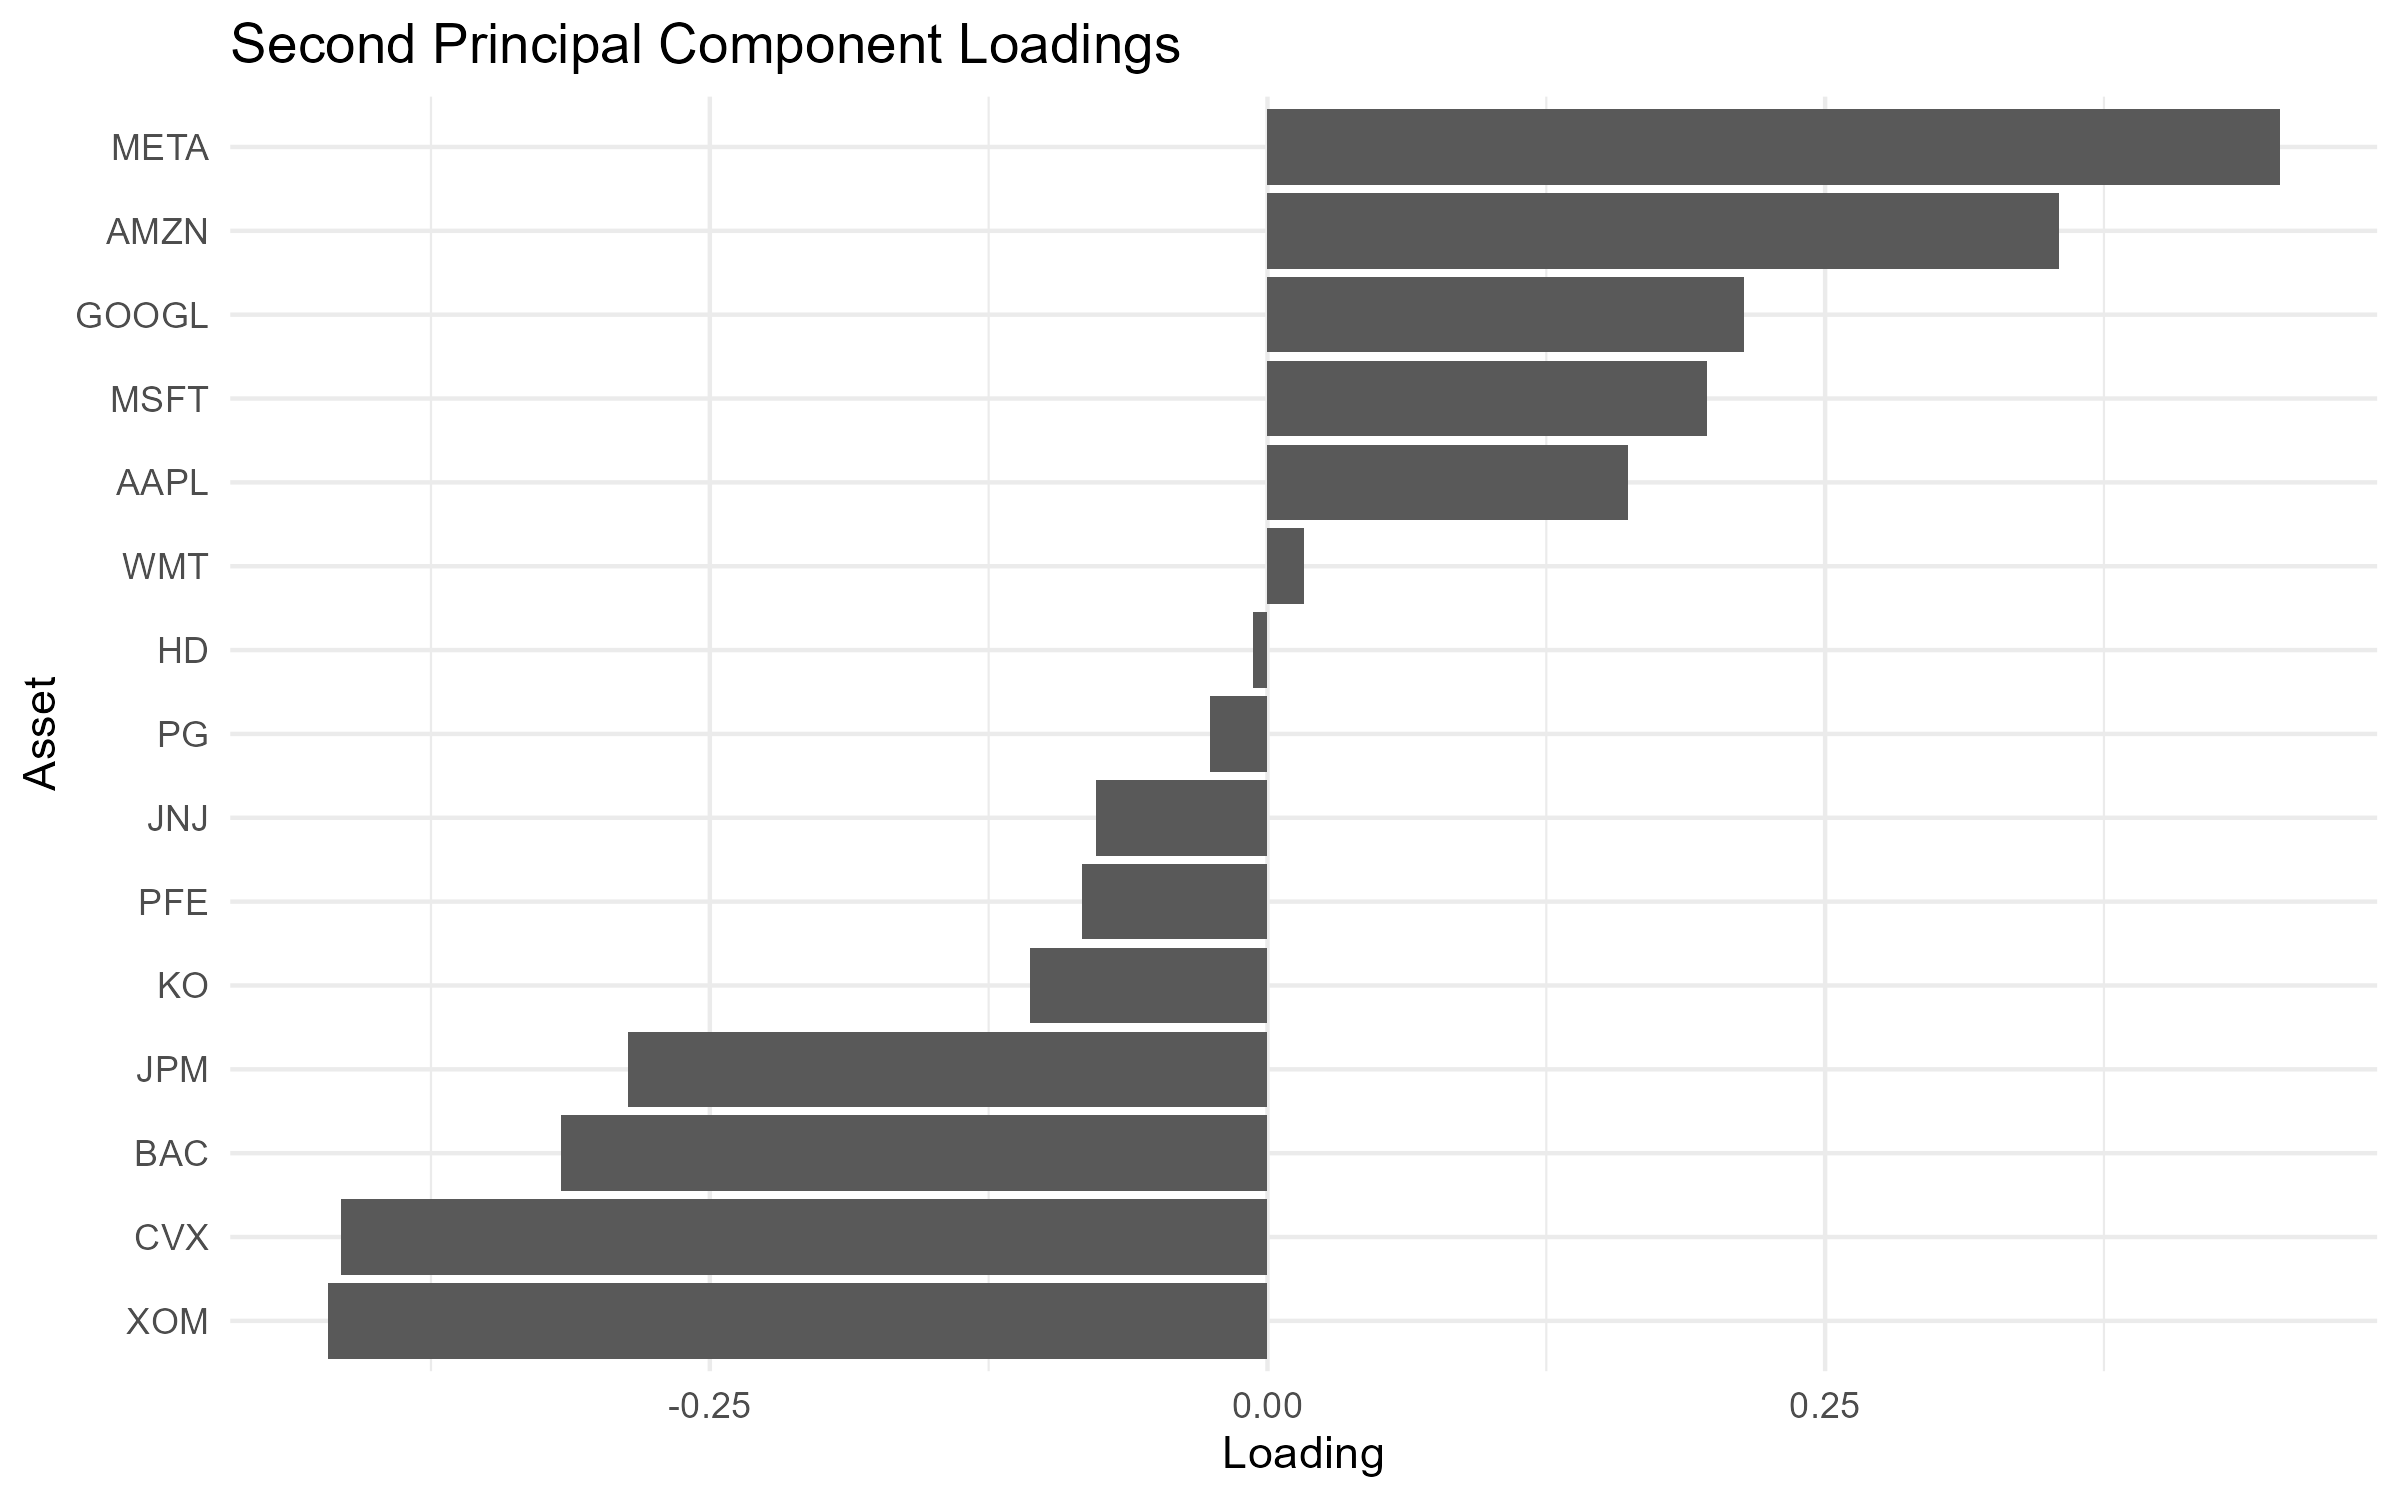
\includegraphics[keepaspectratio]{1-quantitative-finance/../notebooks-and-scripts/1-quantitative-finance/2-unsupervised-learning-for-asset-allocation/r/1-unsupervised-learning-for-asset-allocation-figures/pc2-loadings.png}}

}

\caption{\label{fig-pc2-loadings}Loadings of the second principal
component obtained from PCA, highlighting contrasting sectoral exposures
and latent diversification patterns within the asset universe.}

\end{figure}%

Following the PCA analysis, hierarchical clustering was applied using
the correlation-based distance metric described previously. The
clustering procedure organizes assets according to statistical
similarity, producing a hierarchical representation of the market
structure.

The resulting dendrogram is presented in
Figure~\ref{fig-hierarchical-clustering-dendrogram}.

\begin{figure}

\centering{

\pandocbounded{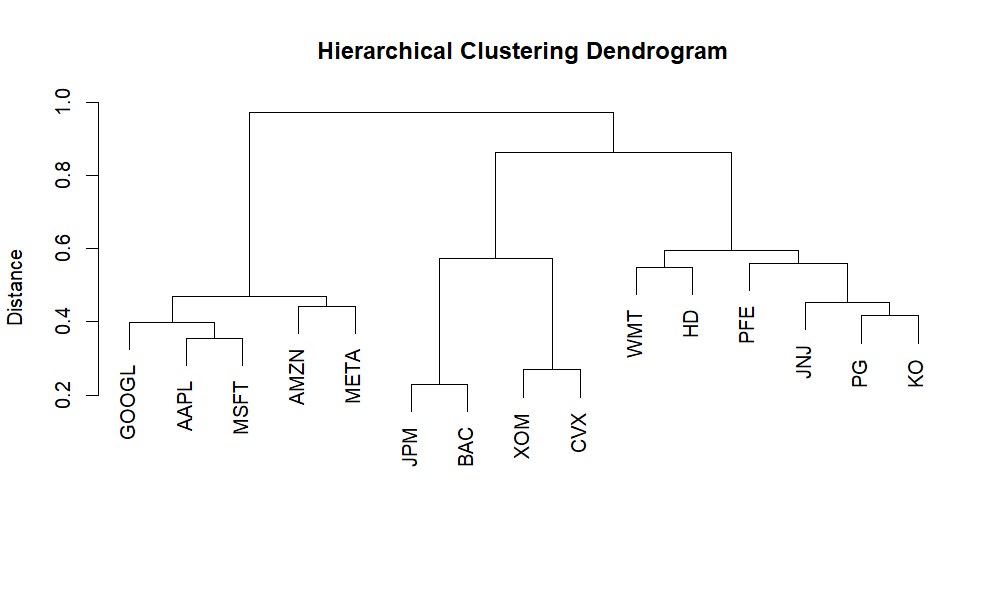
\includegraphics[keepaspectratio]{1-quantitative-finance/../notebooks-and-scripts/1-quantitative-finance/2-unsupervised-learning-for-asset-allocation/r/1-unsupervised-learning-for-asset-allocation-figures/hierarchical-clustering-dendrogram.png}}

}

\caption{\label{fig-hierarchical-clustering-dendrogram}Hierarchical
clustering dendrogram of the asset universe based on return
correlations, revealing sectoral similarity structures used in the
Hierarchical Risk Parity (HRP) allocation process.}

\end{figure}%

The hierarchical organization becomes even more evident after reordering
the correlation matrix according to the clustering structure, as shown
in Figure~\ref{fig-clustered-correlation-matrix}.

\begin{figure}

\centering{

\pandocbounded{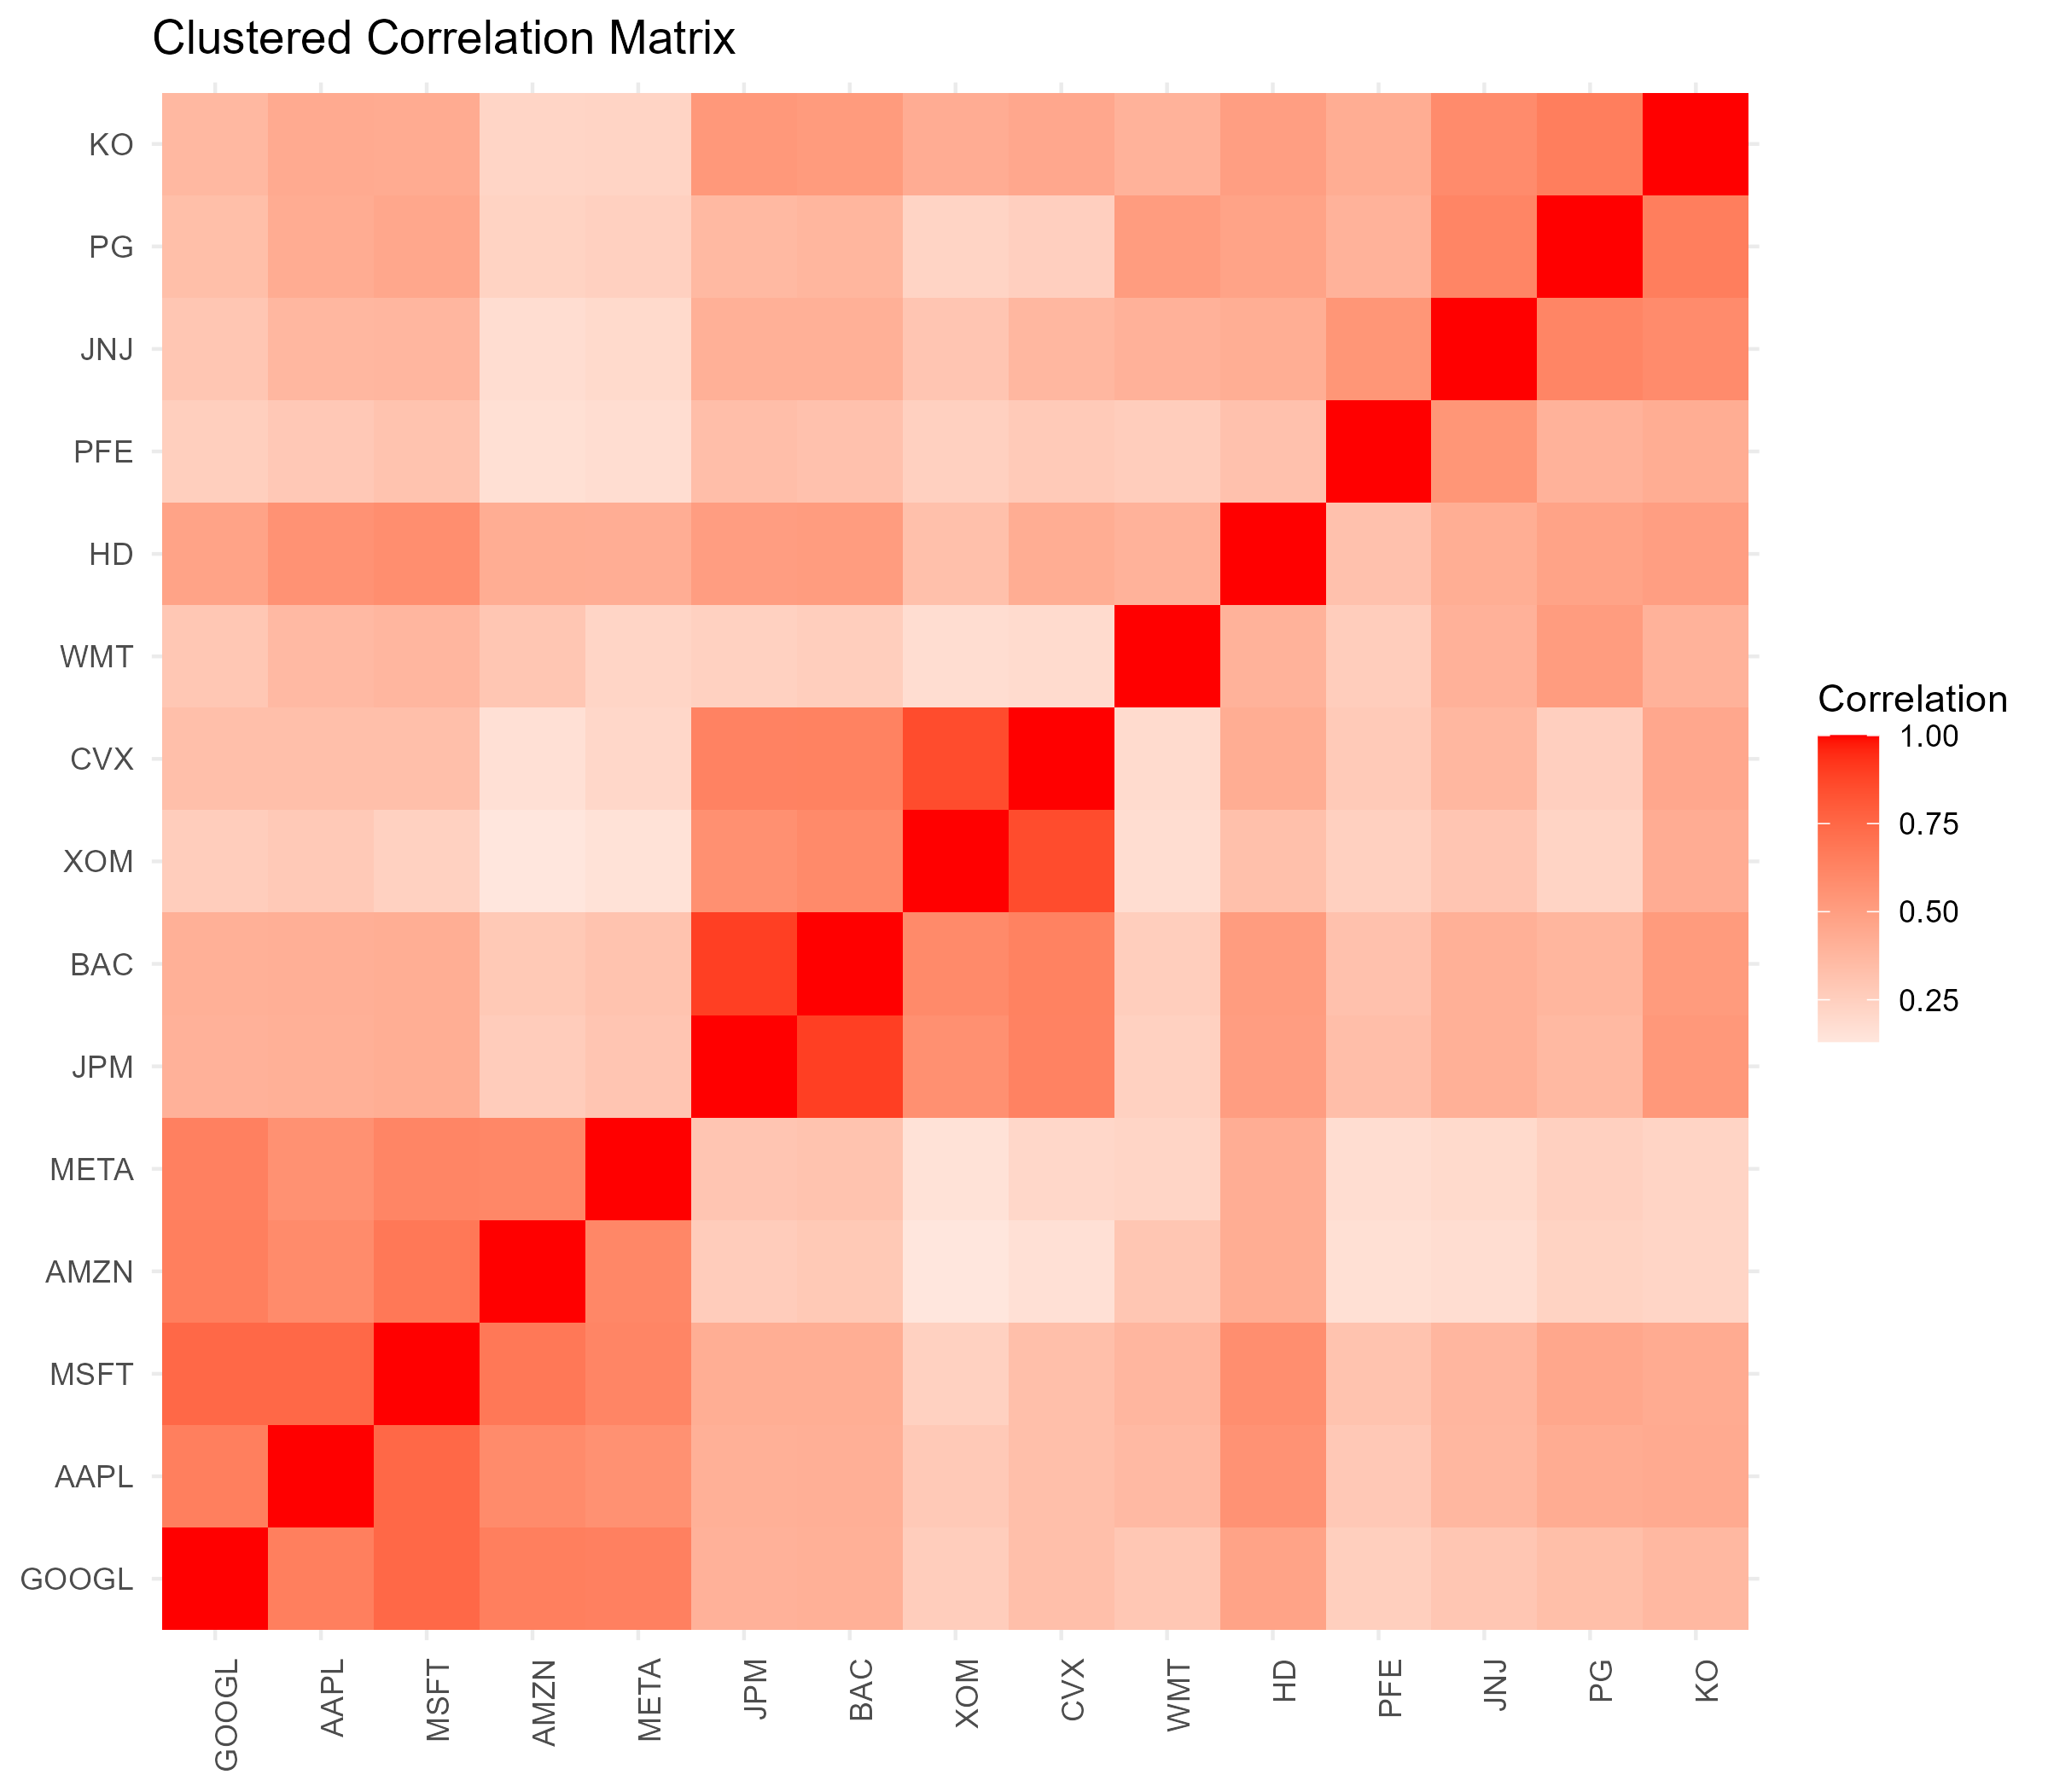
\includegraphics[keepaspectratio]{1-quantitative-finance/../notebooks-and-scripts/1-quantitative-finance/2-unsupervised-learning-for-asset-allocation/r/1-unsupervised-learning-for-asset-allocation-figures/clustered-correlation-matrix.png}}

}

\caption{\label{fig-clustered-correlation-matrix}Clustered correlation
matrix of asset returns, highlighting sectoral structure and similarity
patterns used in the hierarchical portfolio construction process.}

\end{figure}%

Several economically intuitive clusters emerge naturally from the data.
Technology firms tend to cluster together, energy companies form a
separate branch, and defensive sectors exhibit their own hierarchical
relationships.

Portfolio construction was then performed using the Hierarchical Risk
Parity (HRP) allocation framework. For comparison purposes, an equally
weighted portfolio was used as a benchmark throughout the analysis.

The equal-weight allocation is shown in
Figure~\ref{fig-equal-weight-portfolio}.

\begin{figure}

\centering{

\pandocbounded{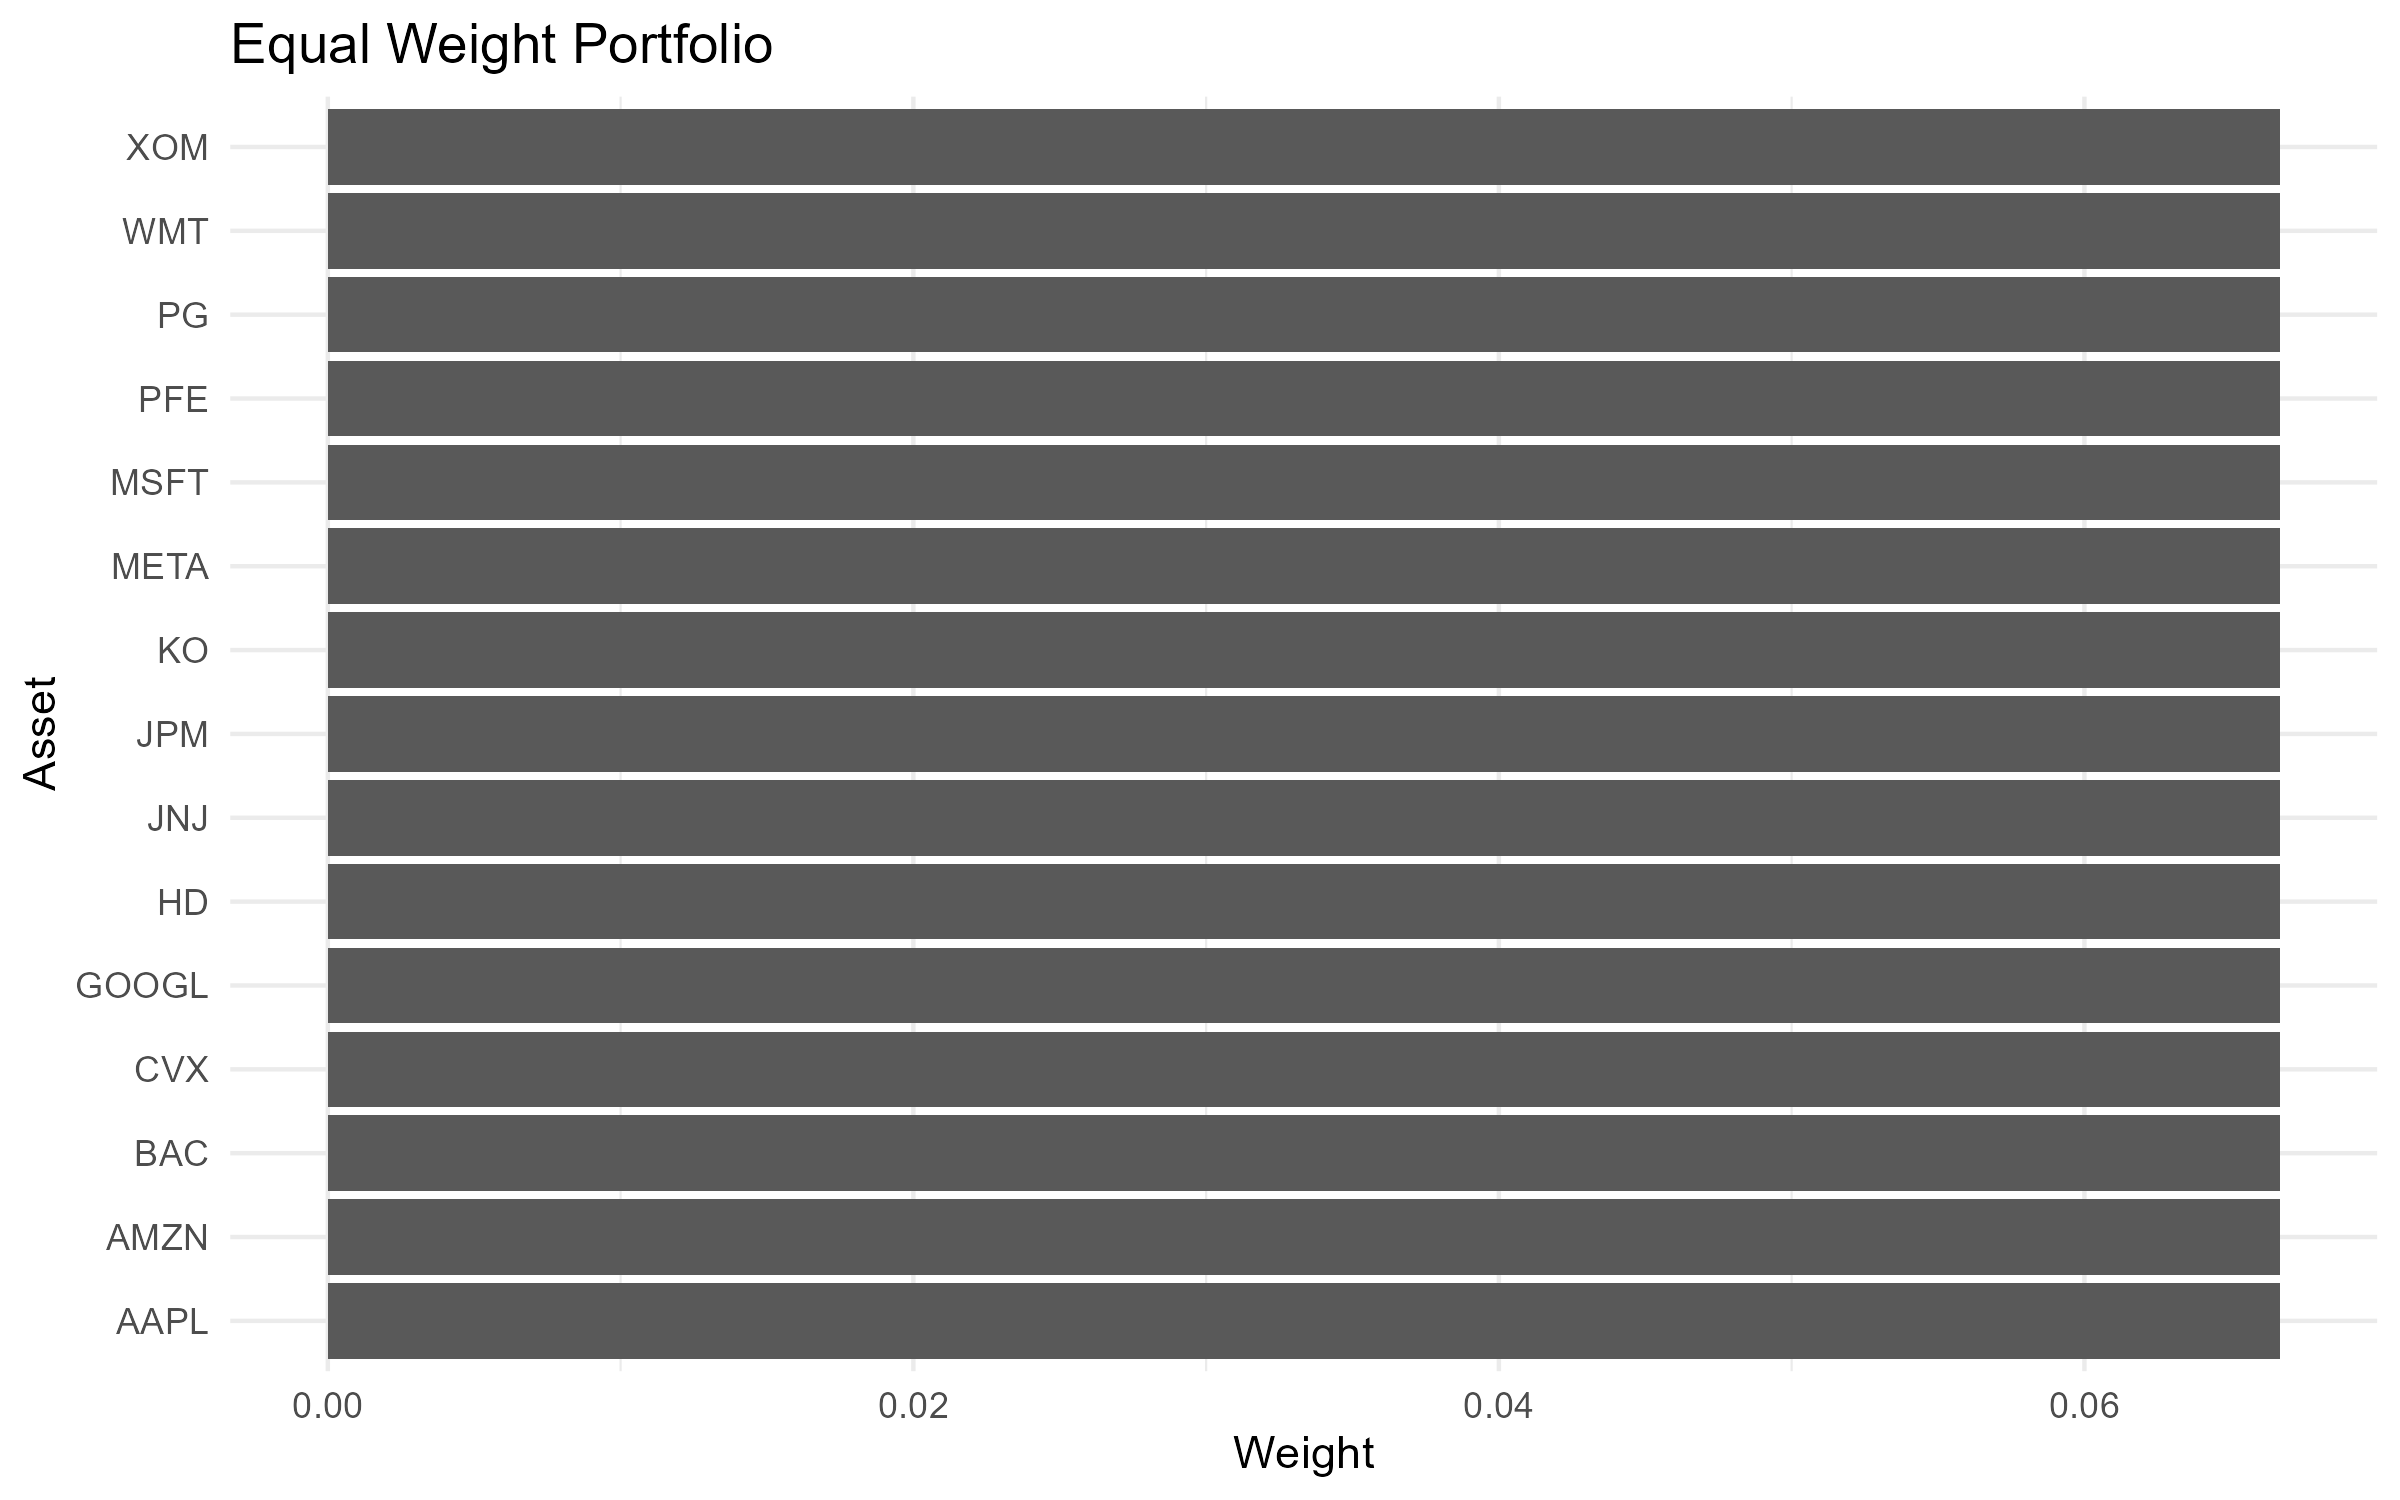
\includegraphics[keepaspectratio]{1-quantitative-finance/../notebooks-and-scripts/1-quantitative-finance/2-unsupervised-learning-for-asset-allocation/r/1-unsupervised-learning-for-asset-allocation-figures/equal-weight-portfolio.png}}

}

\caption{\label{fig-equal-weight-portfolio}Equal-weight portfolio
allocation assigning identical weights to all assets in the investment
universe.}

\end{figure}%

The HRP allocation produced a substantially different weighting
structure. The largest portfolio weights were assigned to JNJ, KO, PG,
and WMT, while exposure to several technology, financial, and energy
assets was reduced relative to the equal-weight benchmark.

\begin{longtable}[]{@{}lc@{}}
\caption{Final portfolio weights obtained using the Hierarchical Risk
Parity (HRP) allocation method. }\label{tbl-hrp-weights}\tabularnewline
\toprule\noalign{}
Asset & Weight \\
\midrule\noalign{}
\endfirsthead
\toprule\noalign{}
Asset & Weight \\
\midrule\noalign{}
\endhead
\bottomrule\noalign{}
\endlastfoot
JNJ & 0.1285 \\
KO & 0.1171 \\
PG & 0.1158 \\
WMT & 0.1127 \\
GOOGL & 0.0705 \\
HD & 0.0689 \\
PFE & 0.0657 \\
JPM & 0.0471 \\
MSFT & 0.0457 \\
AMZN & 0.0439 \\
AAPL & 0.0424 \\
BAC & 0.0390 \\
XOM & 0.0386 \\
CVX & 0.0360 \\
META & 0.0282 \\
\end{longtable}

The resulting allocation is visualized in
Figure~\ref{fig-hrp-portfolio-weights}.

\begin{figure}

\centering{

\pandocbounded{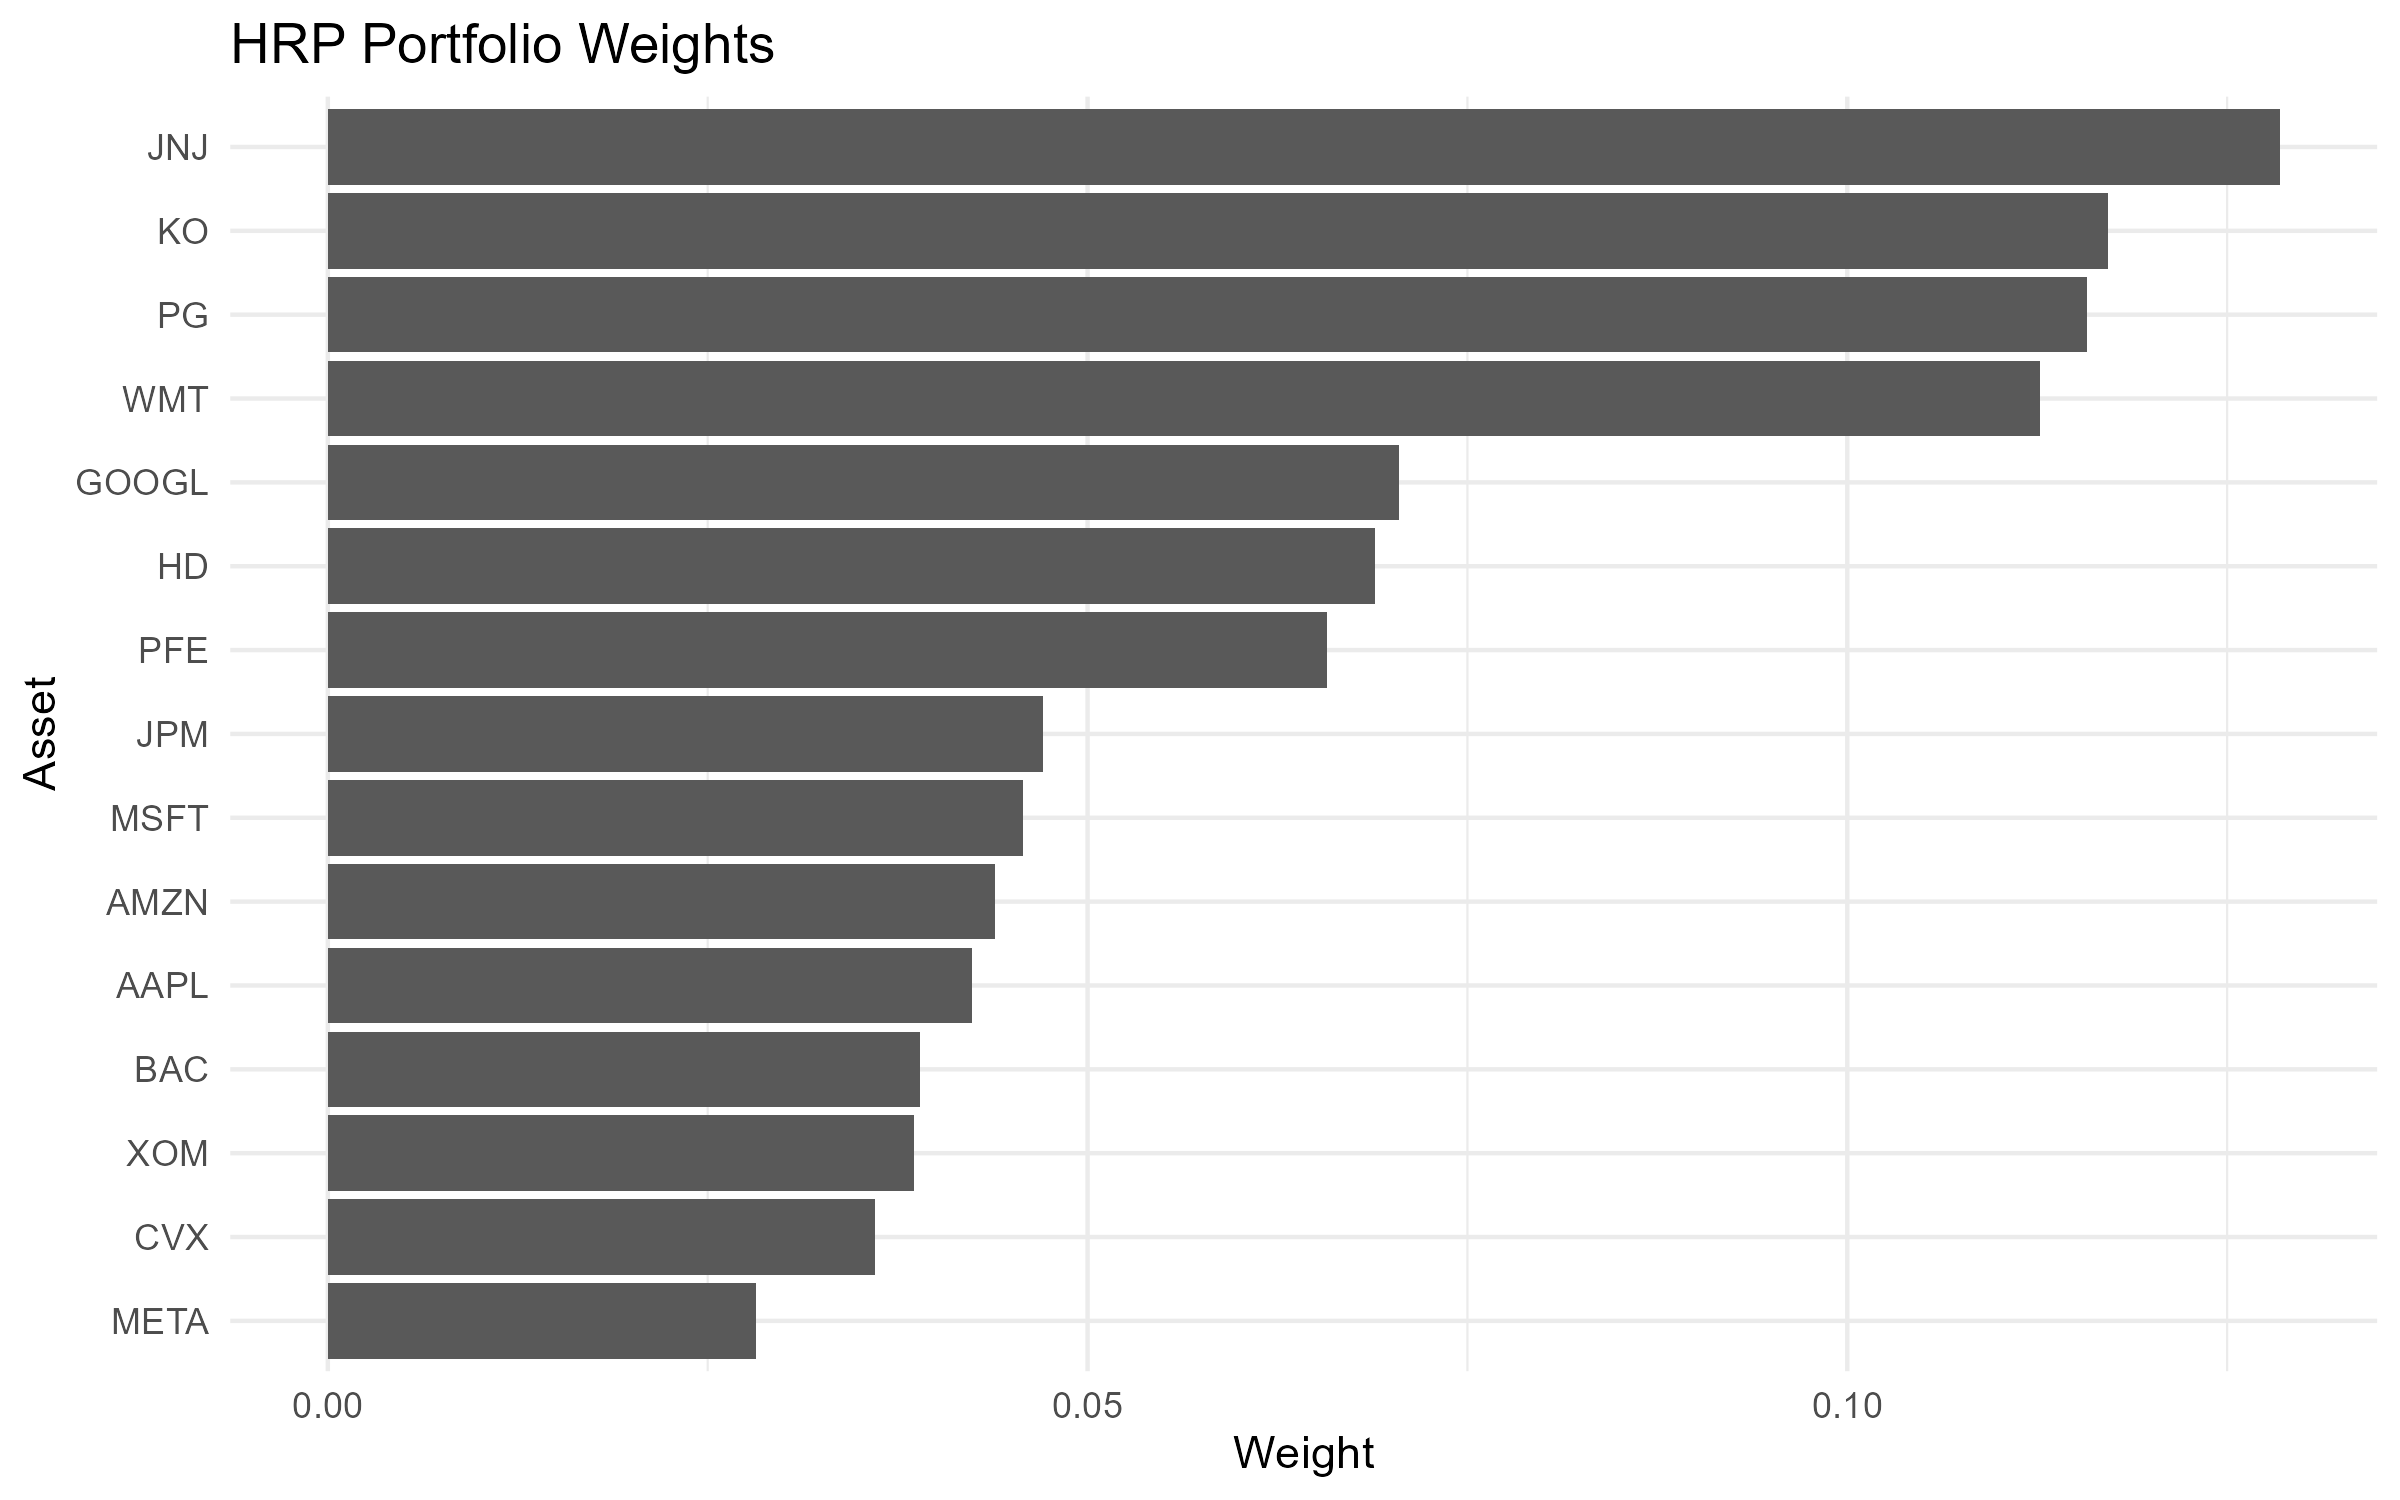
\includegraphics[keepaspectratio]{1-quantitative-finance/../notebooks-and-scripts/1-quantitative-finance/2-unsupervised-learning-for-asset-allocation/r/1-unsupervised-learning-for-asset-allocation-figures/hrp-portfolio-weights.png}}

}

\caption{\label{fig-hrp-portfolio-weights}Portfolio weights obtained
using the Hierarchical Risk Parity (HRP) allocation method, reflecting
the hierarchical correlation structure and risk diversification across
assets.}

\end{figure}%

A direct comparison between the equal-weight benchmark and the HRP
allocation is shown in Figure~\ref{fig-portfolio-weight-comparison} and
Table~\ref{tbl-portfolio-weight-comparison}.

The differences between the two allocations are visible both at the
individual asset level and across sectors. The larger weights assigned
to JNJ, KO, PG, and WMT are broadly consistent with the lower volatility
and correlation characteristics often associated with defensive sectors.

\begin{figure}

\centering{

\pandocbounded{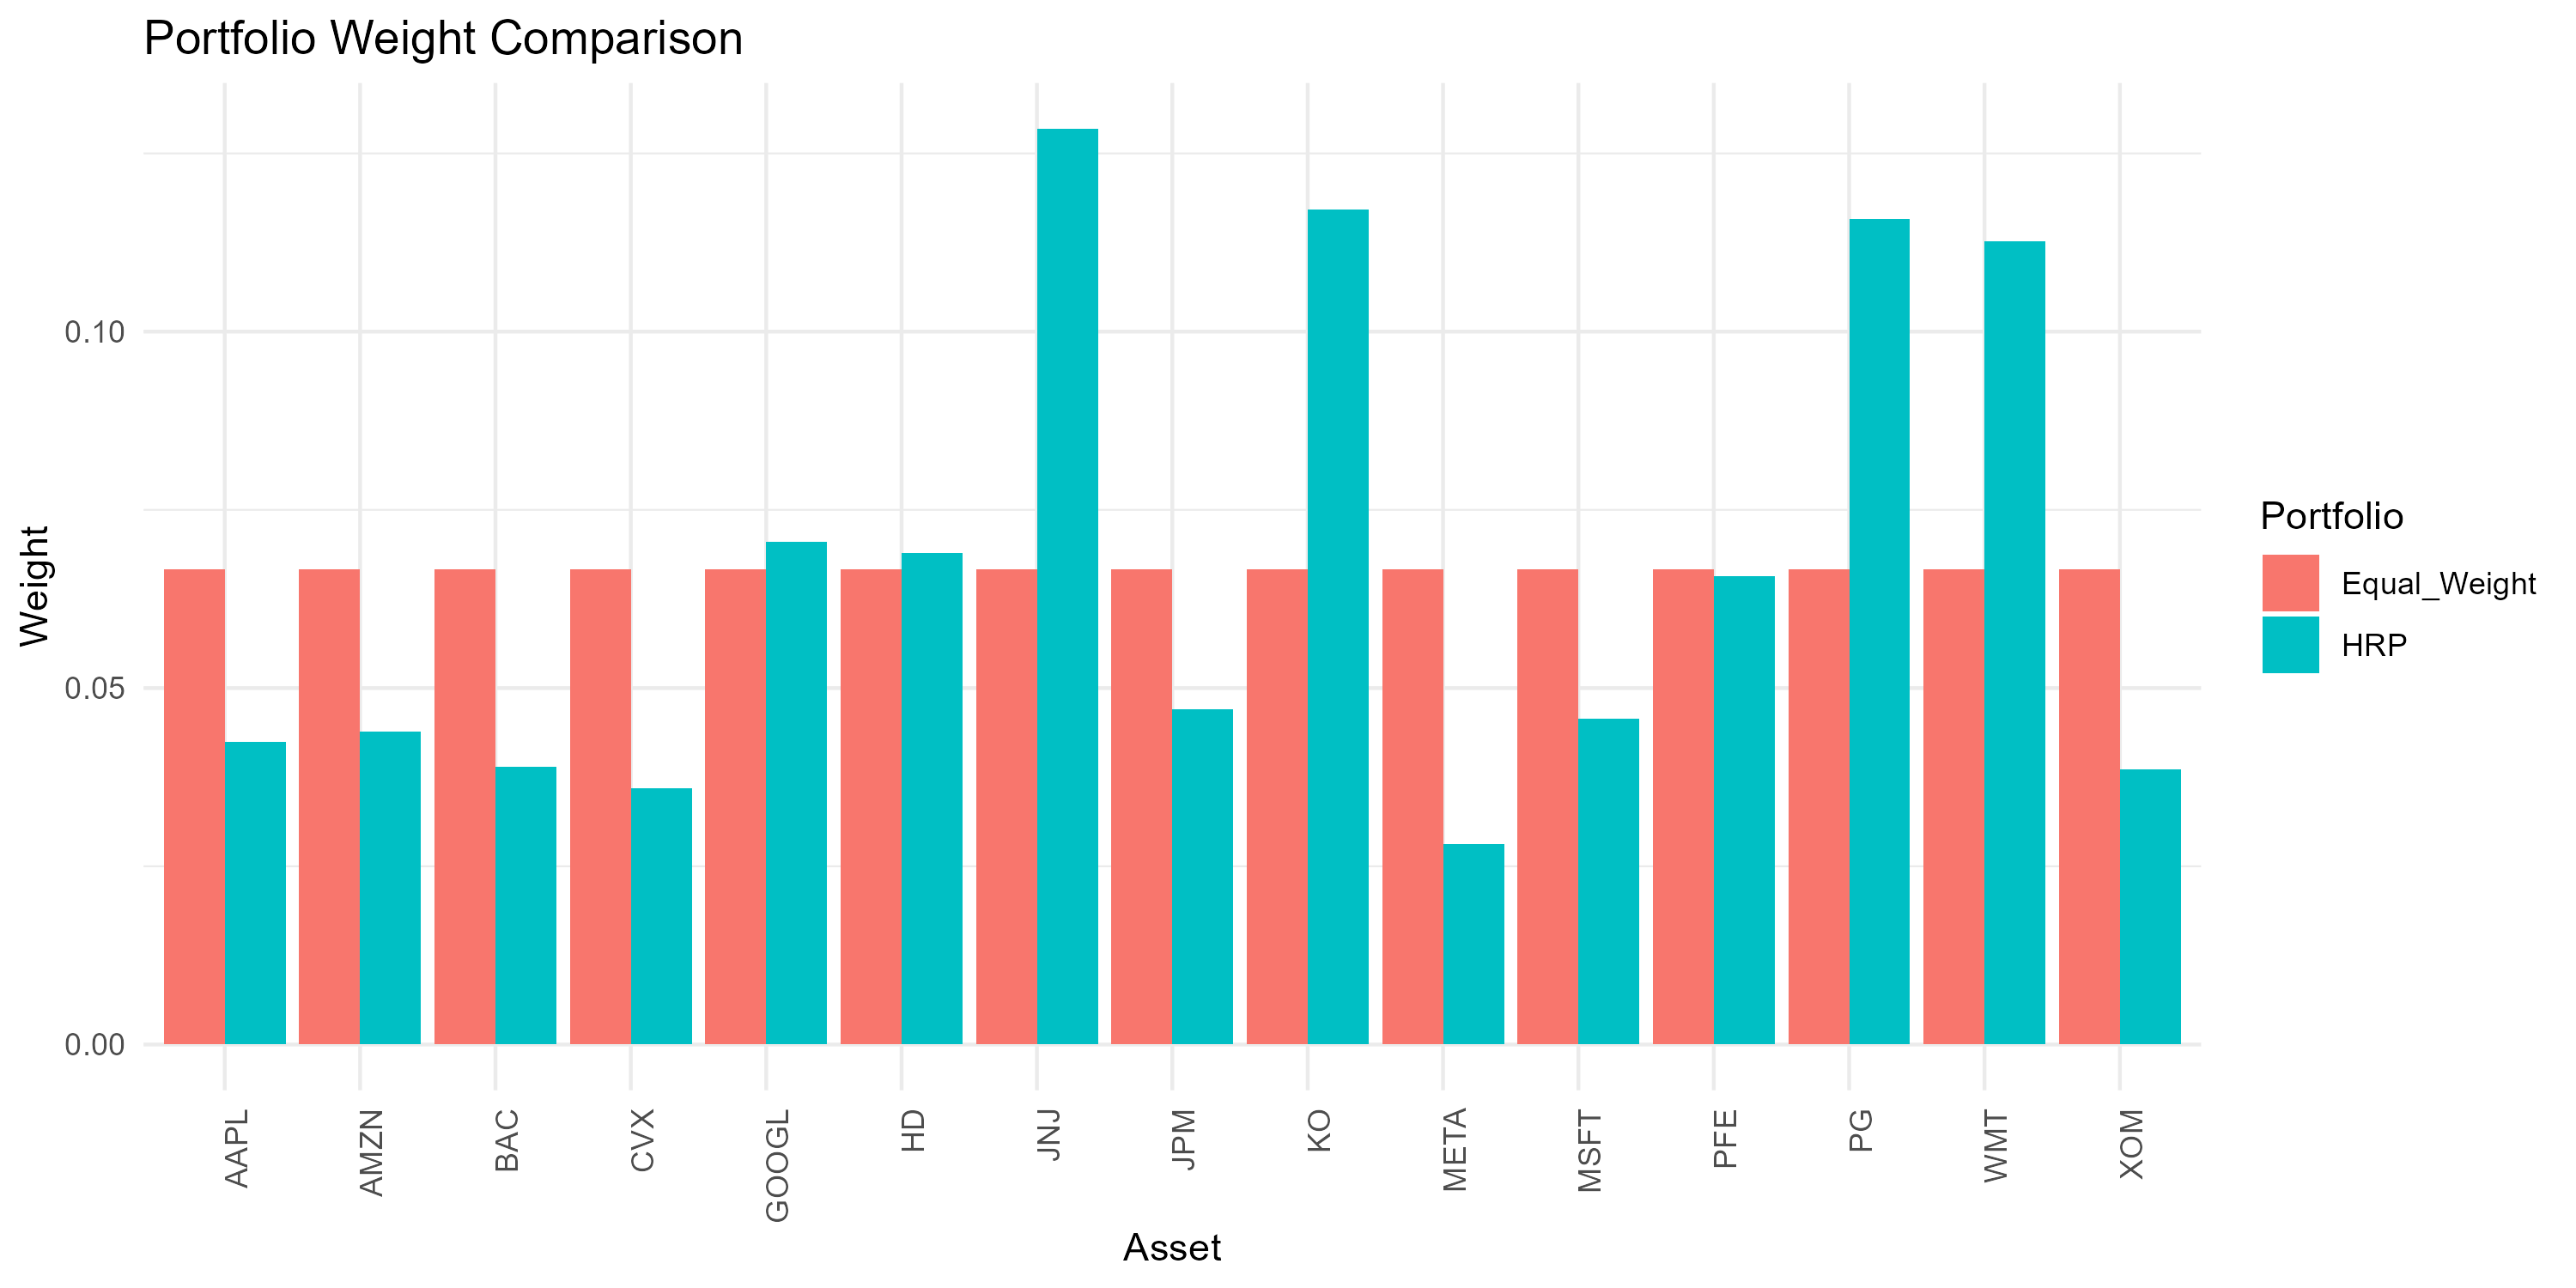
\includegraphics[keepaspectratio]{1-quantitative-finance/../notebooks-and-scripts/1-quantitative-finance/2-unsupervised-learning-for-asset-allocation/r/1-unsupervised-learning-for-asset-allocation-figures/portfolio-weight-comparison.png}}

}

\caption{\label{fig-portfolio-weight-comparison}Comparison between
equal-weight and Hierarchical Risk Parity (HRP) portfolio allocations,
highlighting how the HRP framework redistributes exposure according to
the hierarchical correlation and risk structure of the asset universe.}

\end{figure}%

\begin{longtable}[]{@{}ccc@{}}
\caption{Comparison between equal-weight portfolio allocation and
Hierarchical Risk Parity (HRP) portfolio weights.
}\label{tbl-portfolio-weight-comparison}\tabularnewline
\toprule\noalign{}
Asset & Equal Weight & HRP \\
\midrule\noalign{}
\endfirsthead
\toprule\noalign{}
Asset & Equal Weight & HRP \\
\midrule\noalign{}
\endhead
\bottomrule\noalign{}
\endlastfoot
AAPL & 0.0667 & 0.0424 \\
MSFT & 0.0667 & 0.0457 \\
GOOGL & 0.0667 & 0.0705 \\
AMZN & 0.0667 & 0.0439 \\
META & 0.0667 & 0.0282 \\
JPM & 0.0667 & 0.0471 \\
BAC & 0.0667 & 0.0390 \\
XOM & 0.0667 & 0.0386 \\
CVX & 0.0667 & 0.0360 \\
JNJ & 0.0667 & 0.1285 \\
PFE & 0.0667 & 0.0657 \\
PG & 0.0667 & 0.1158 \\
KO & 0.0667 & 0.1171 \\
WMT & 0.0667 & 0.1127 \\
HD & 0.0667 & 0.0689 \\
\end{longtable}

Risk contributions were also evaluated in order to study how portfolio
risk was distributed across assets under the HRP framework.

\begin{longtable}[]{@{}cc@{}}
\caption{Asset-level risk contributions under the Hierarchical Risk
Parity (HRP) allocation framework.
}\label{tbl-hrp-risk-contribution}\tabularnewline
\toprule\noalign{}
Asset & Risk Contribution \\
\midrule\noalign{}
\endfirsthead
\toprule\noalign{}
Asset & Risk Contribution \\
\midrule\noalign{}
\endhead
\bottomrule\noalign{}
\endlastfoot
KO & 0.001158 \\
JNJ & 0.001111 \\
PG & 0.001090 \\
GOOGL & 0.001007 \\
WMT & 0.000947 \\
HD & 0.000925 \\
JPM & 0.000676 \\
MSFT & 0.000668 \\
PFE & 0.000630 \\
BAC & 0.000620 \\
AAPL & 0.000615 \\
AMZN & 0.000562 \\
CVX & 0.000489 \\
XOM & 0.000450 \\
META & 0.000443 \\
\end{longtable}

The distribution of risk contributions is illustrated in
Figure~\ref{fig-hrp-risk-contribution}.

\begin{figure}

\centering{

\pandocbounded{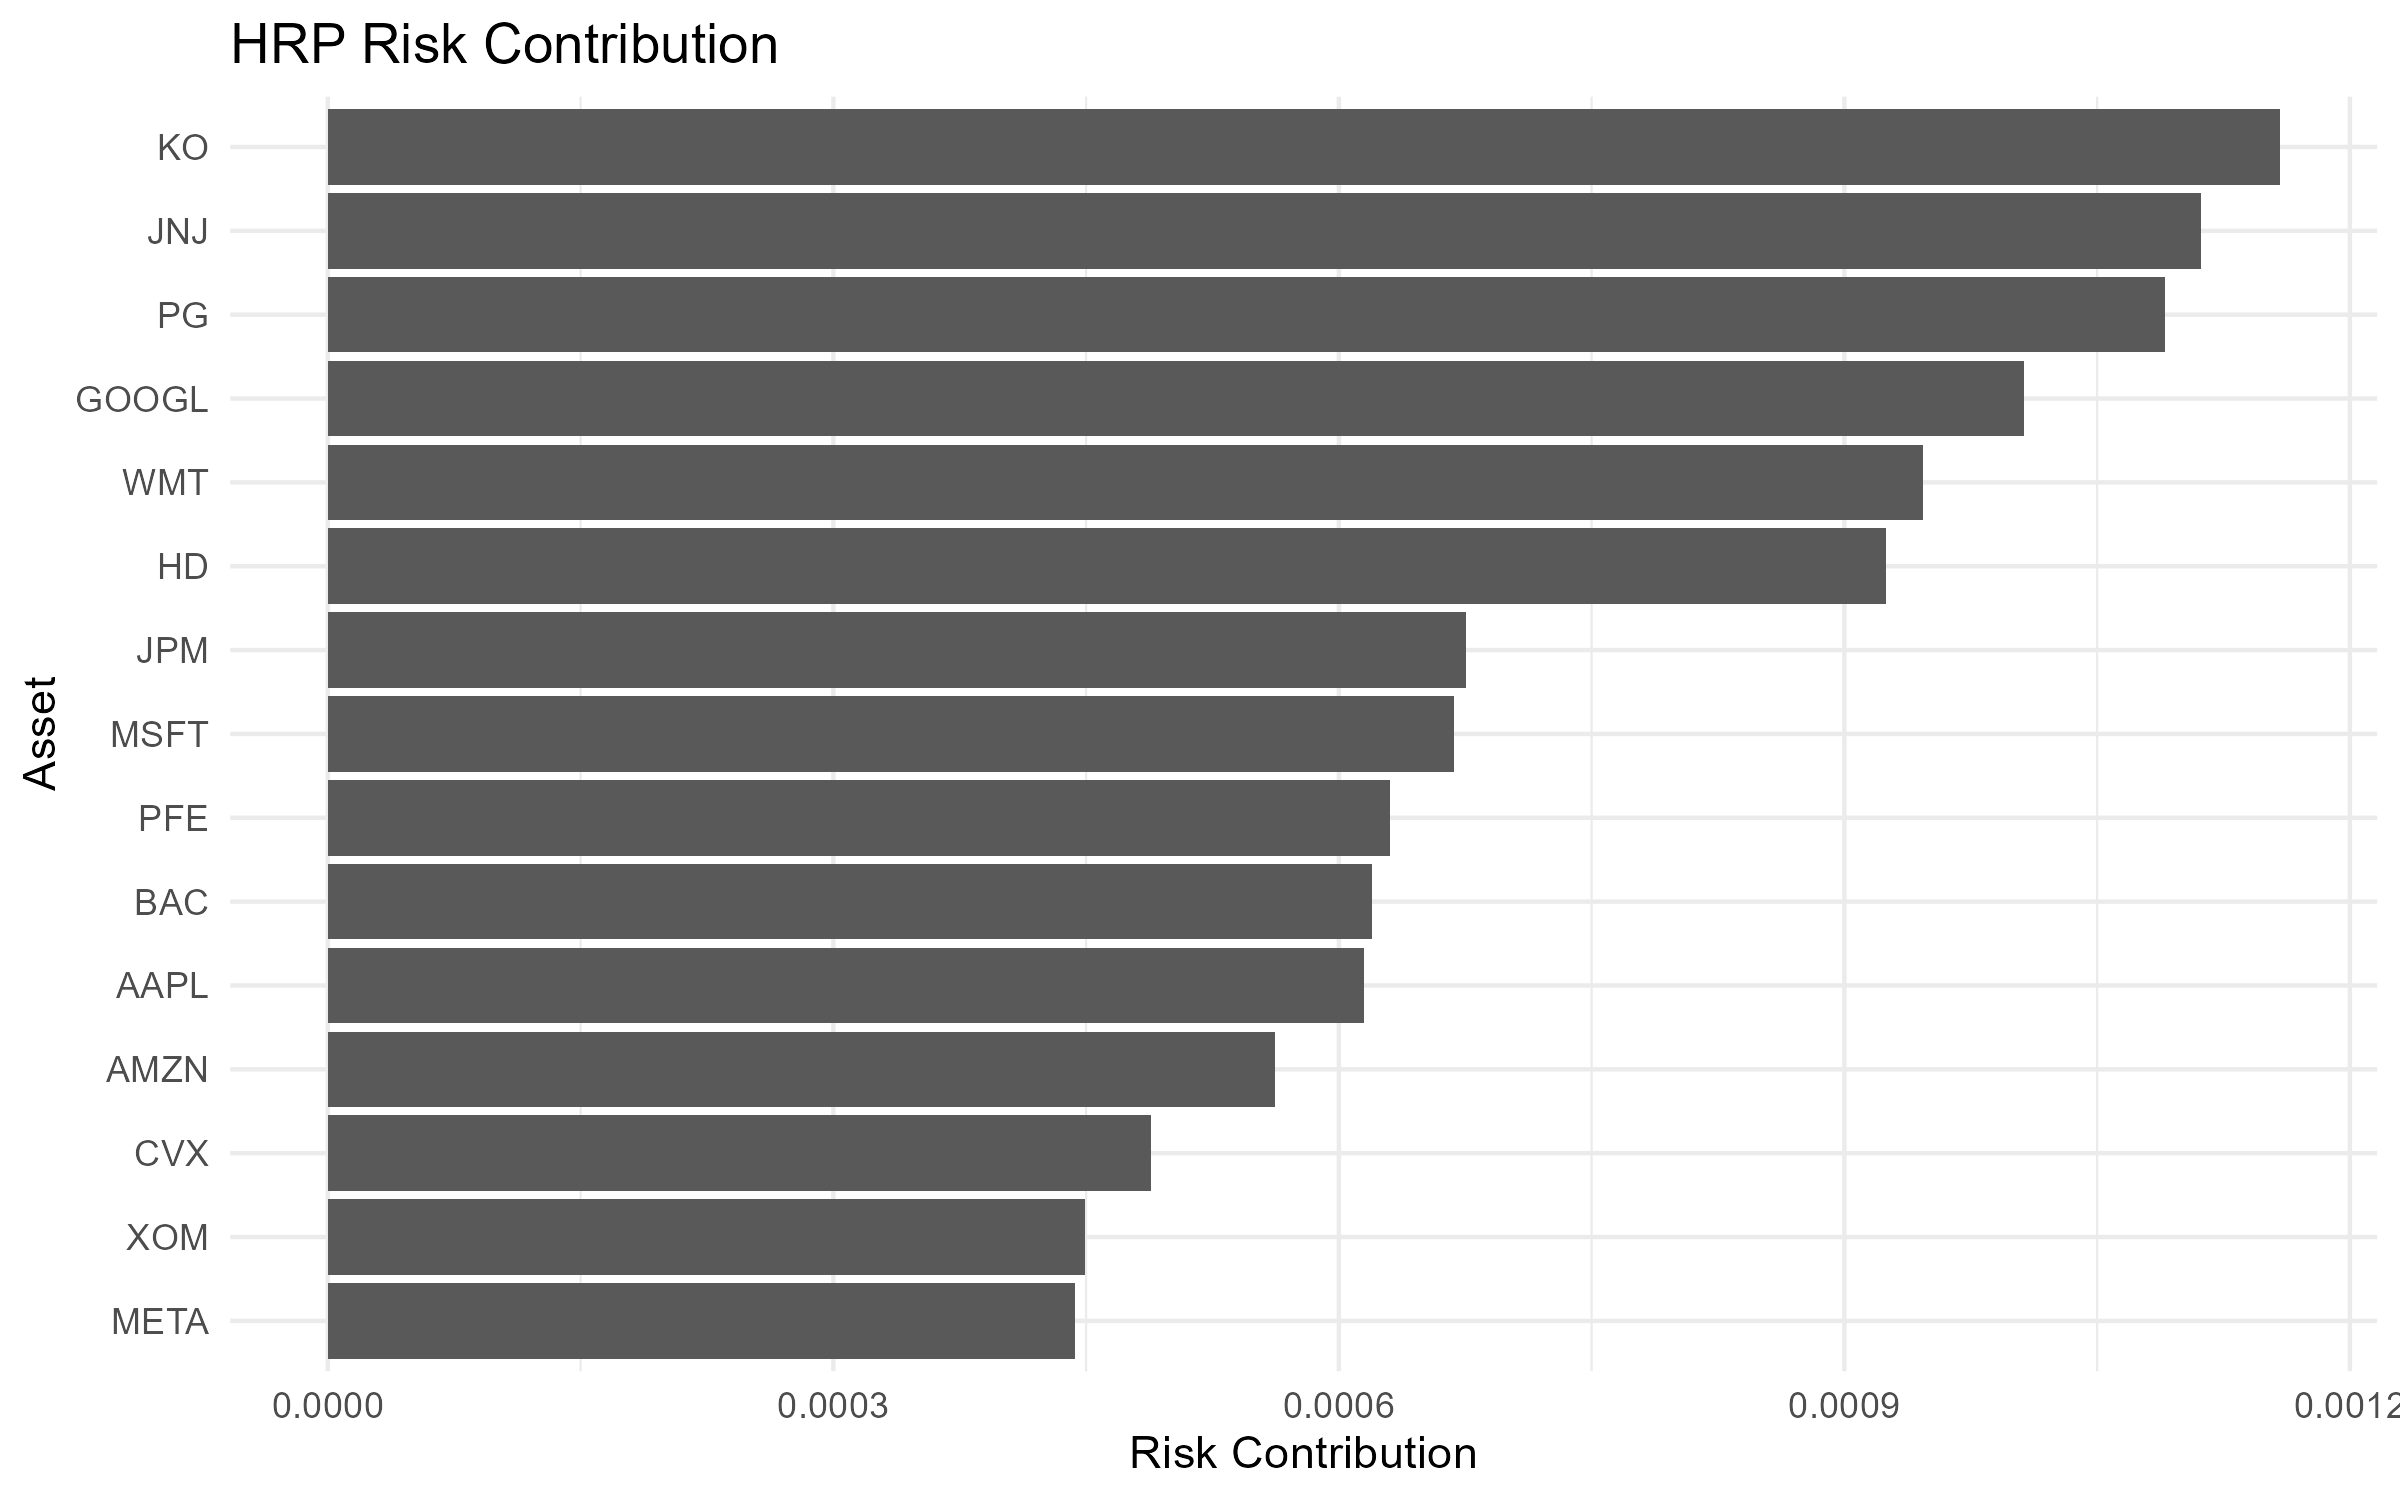
\includegraphics[keepaspectratio]{1-quantitative-finance/../notebooks-and-scripts/1-quantitative-finance/2-unsupervised-learning-for-asset-allocation/r/1-unsupervised-learning-for-asset-allocation-figures/hrp-risk-contribution.png}}

}

\caption{\label{fig-hrp-risk-contribution}Risk contribution of each
asset under the Hierarchical Risk Parity (HRP) allocation, illustrating
how portfolio risk is distributed across the investment universe.}

\end{figure}%

Portfolio performance was evaluated using cumulative returns, rolling
annualized volatility, Sharpe ratio, and maximum drawdown. The
cumulative return dynamics of both portfolio strategies are shown in
Figure~\ref{fig-cumulative-portfolio-returns}.

\begin{figure}

\centering{

\pandocbounded{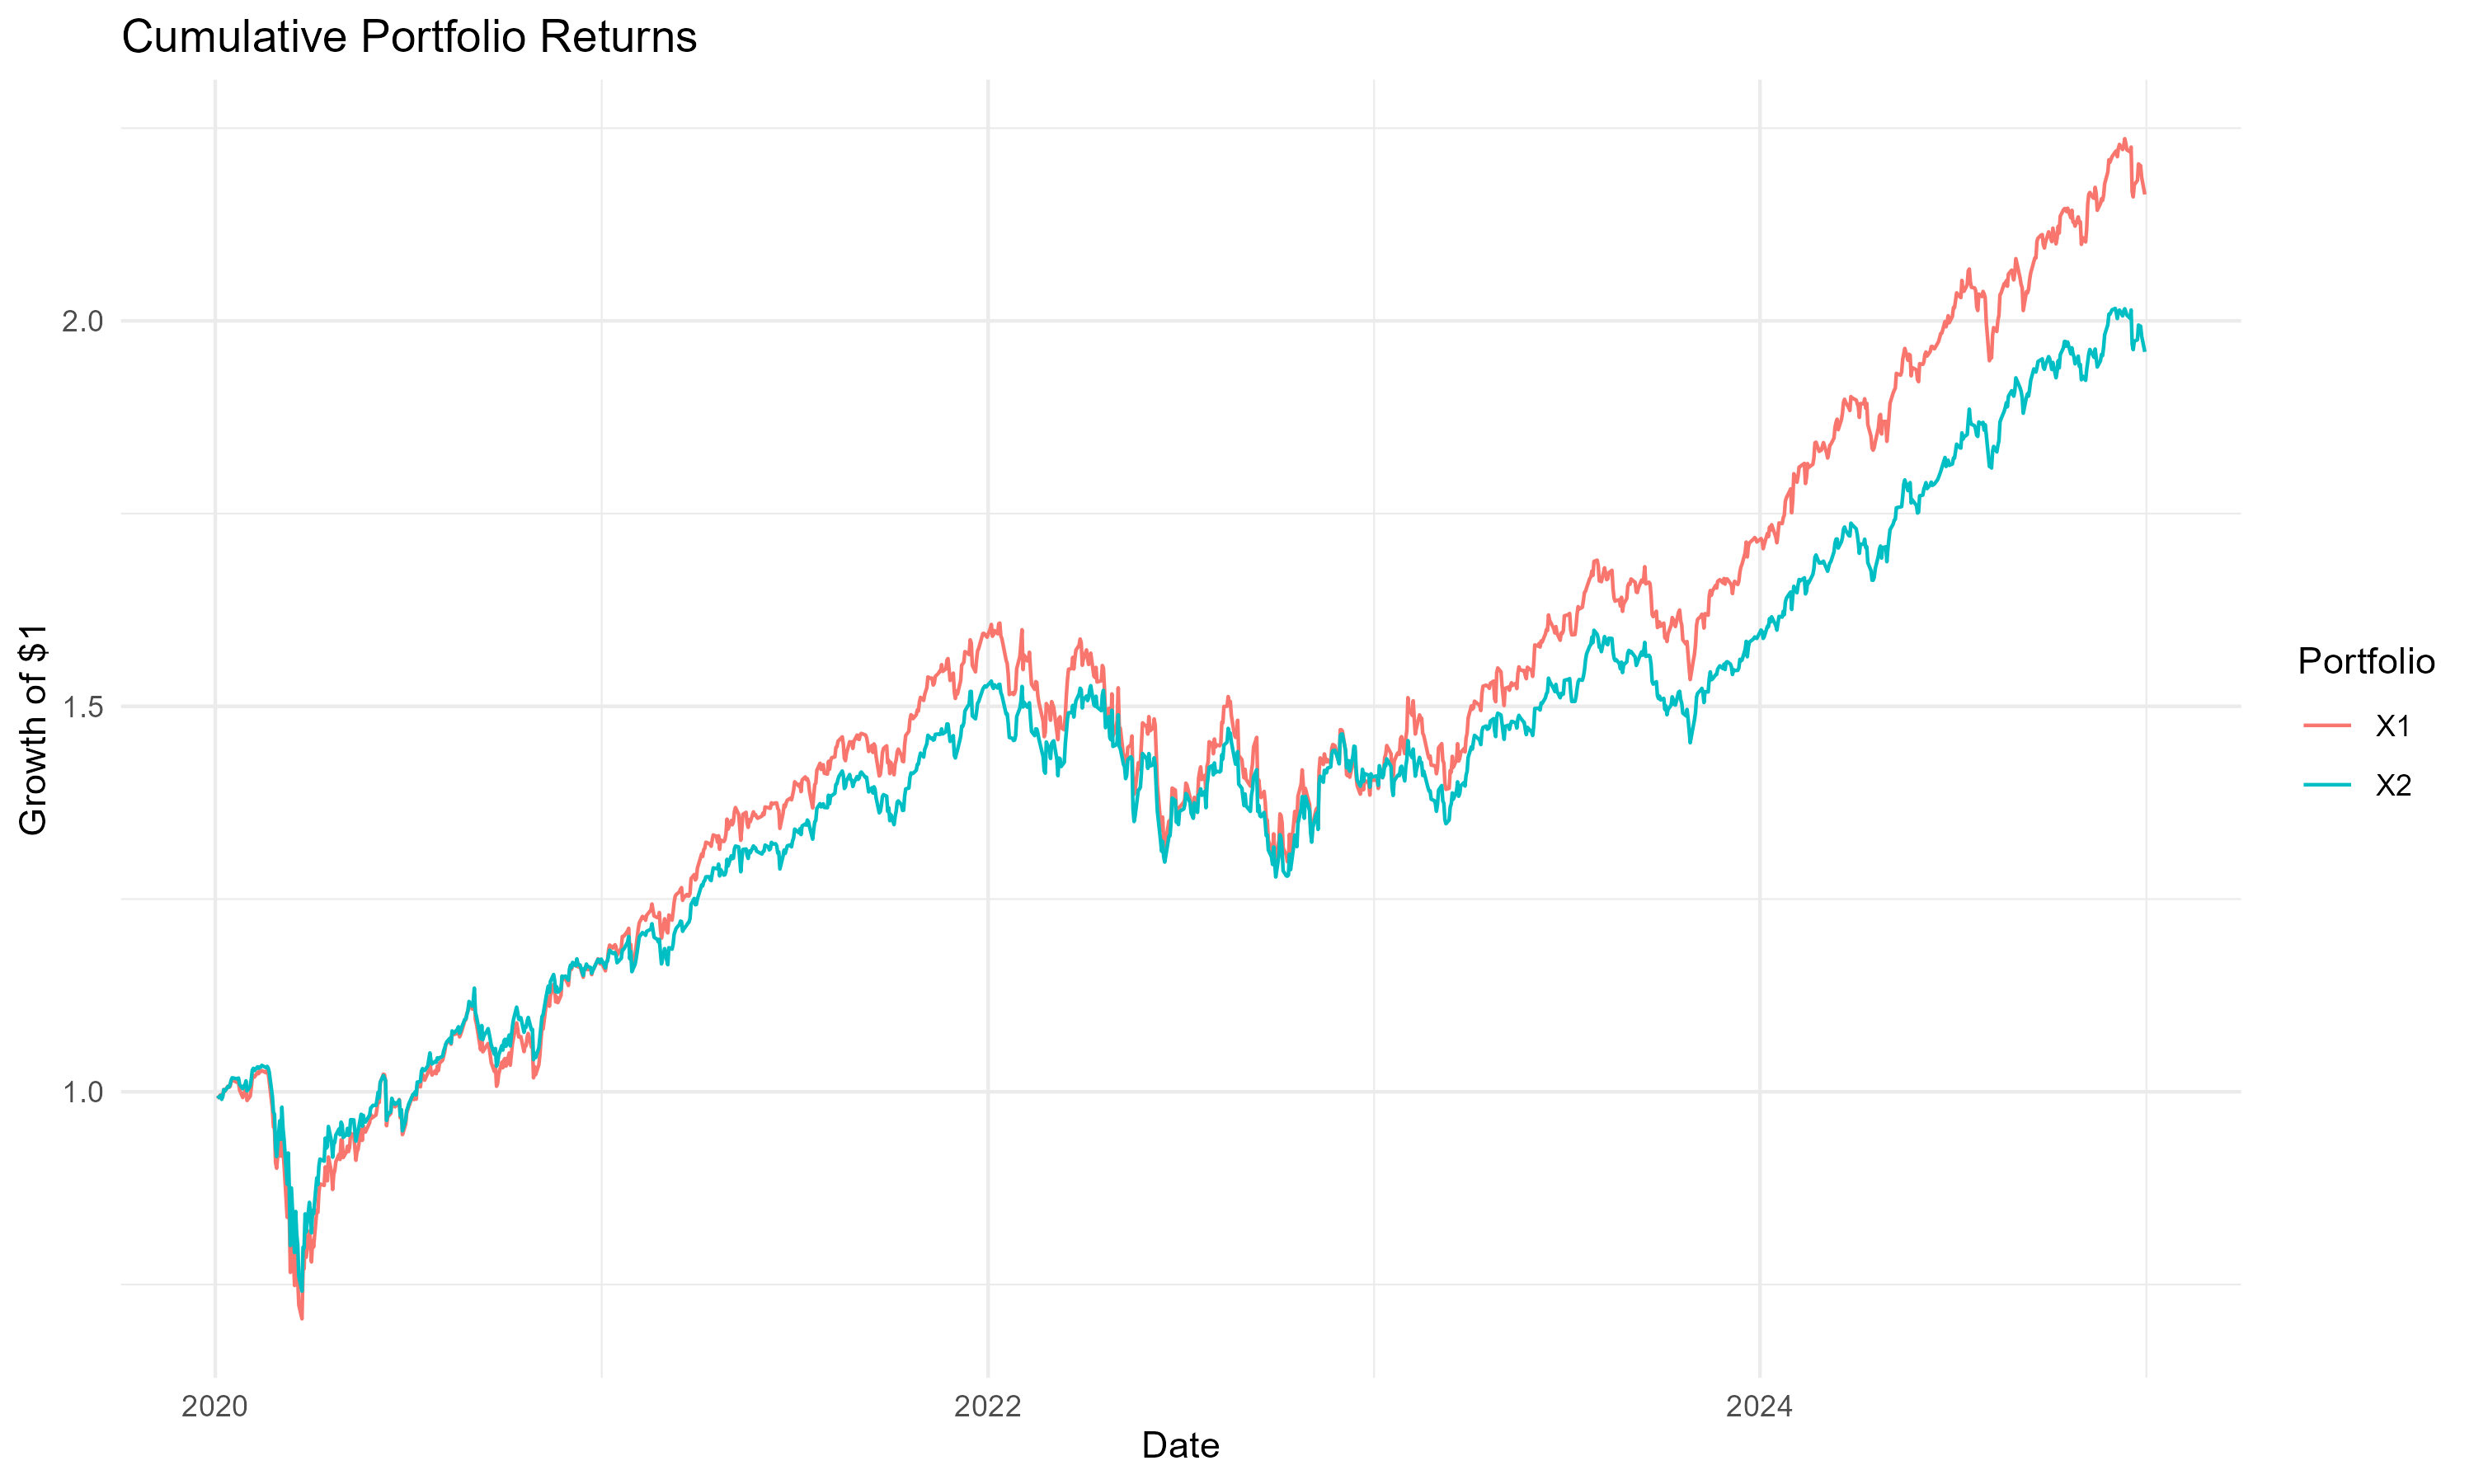
\includegraphics[keepaspectratio]{1-quantitative-finance/../notebooks-and-scripts/1-quantitative-finance/2-unsupervised-learning-for-asset-allocation/r/1-unsupervised-learning-for-asset-allocation-figures/cumulative-portfolio-returns.png}}

}

\caption{\label{fig-cumulative-portfolio-returns}Cumulative returns of
the compared portfolio strategies over the evaluation period,
illustrating differences in long-term growth dynamics and drawdown
behavior.}

\end{figure}%

The temporal evolution of portfolio risk is shown in
Figure~\ref{fig-rolling-annualized-volatility}.

\begin{figure}

\centering{

\pandocbounded{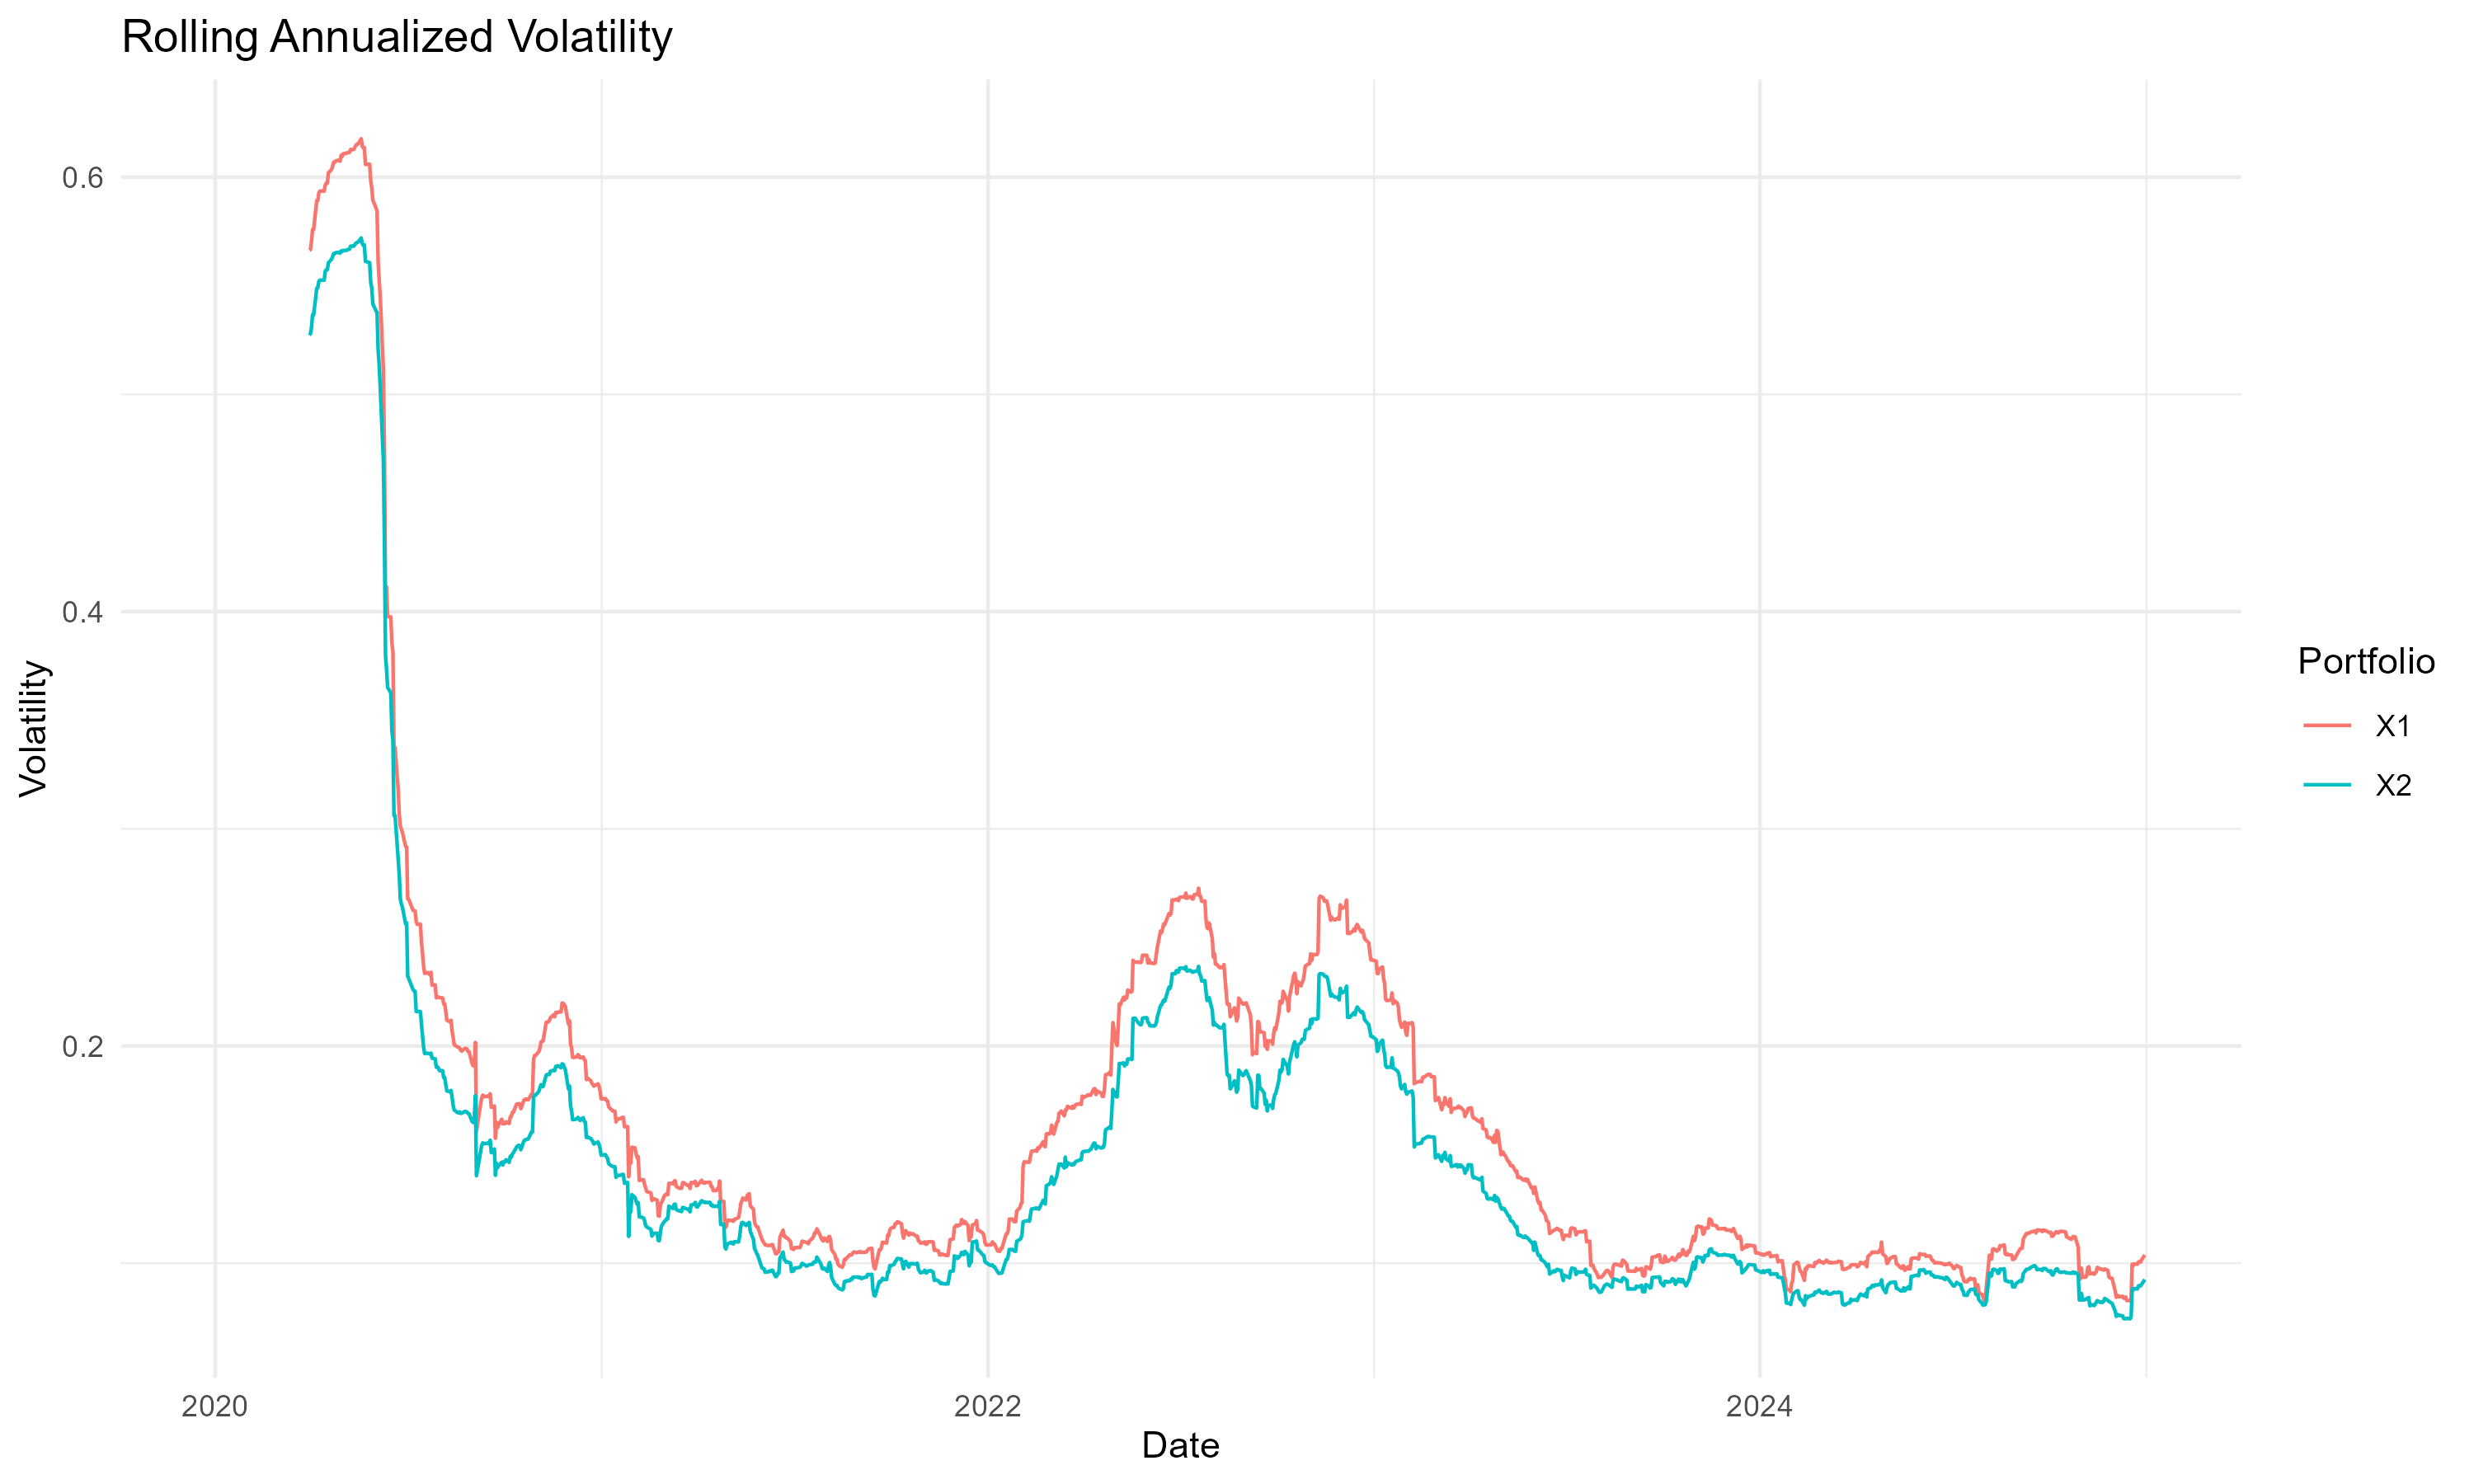
\includegraphics[keepaspectratio]{1-quantitative-finance/../notebooks-and-scripts/1-quantitative-finance/2-unsupervised-learning-for-asset-allocation/r/1-unsupervised-learning-for-asset-allocation-figures/rolling-annualized-volatility.png}}

}

\caption{\label{fig-rolling-annualized-volatility}Rolling annualized
volatility of the portfolio strategies over time, illustrating the
dynamic evolution of portfolio risk under different allocation
frameworks.}

\end{figure}%

Drawdown dynamics were analyzed separately in order to study the
behaviour of both portfolios during periods of market stress.

\begin{figure}

\centering{

\pandocbounded{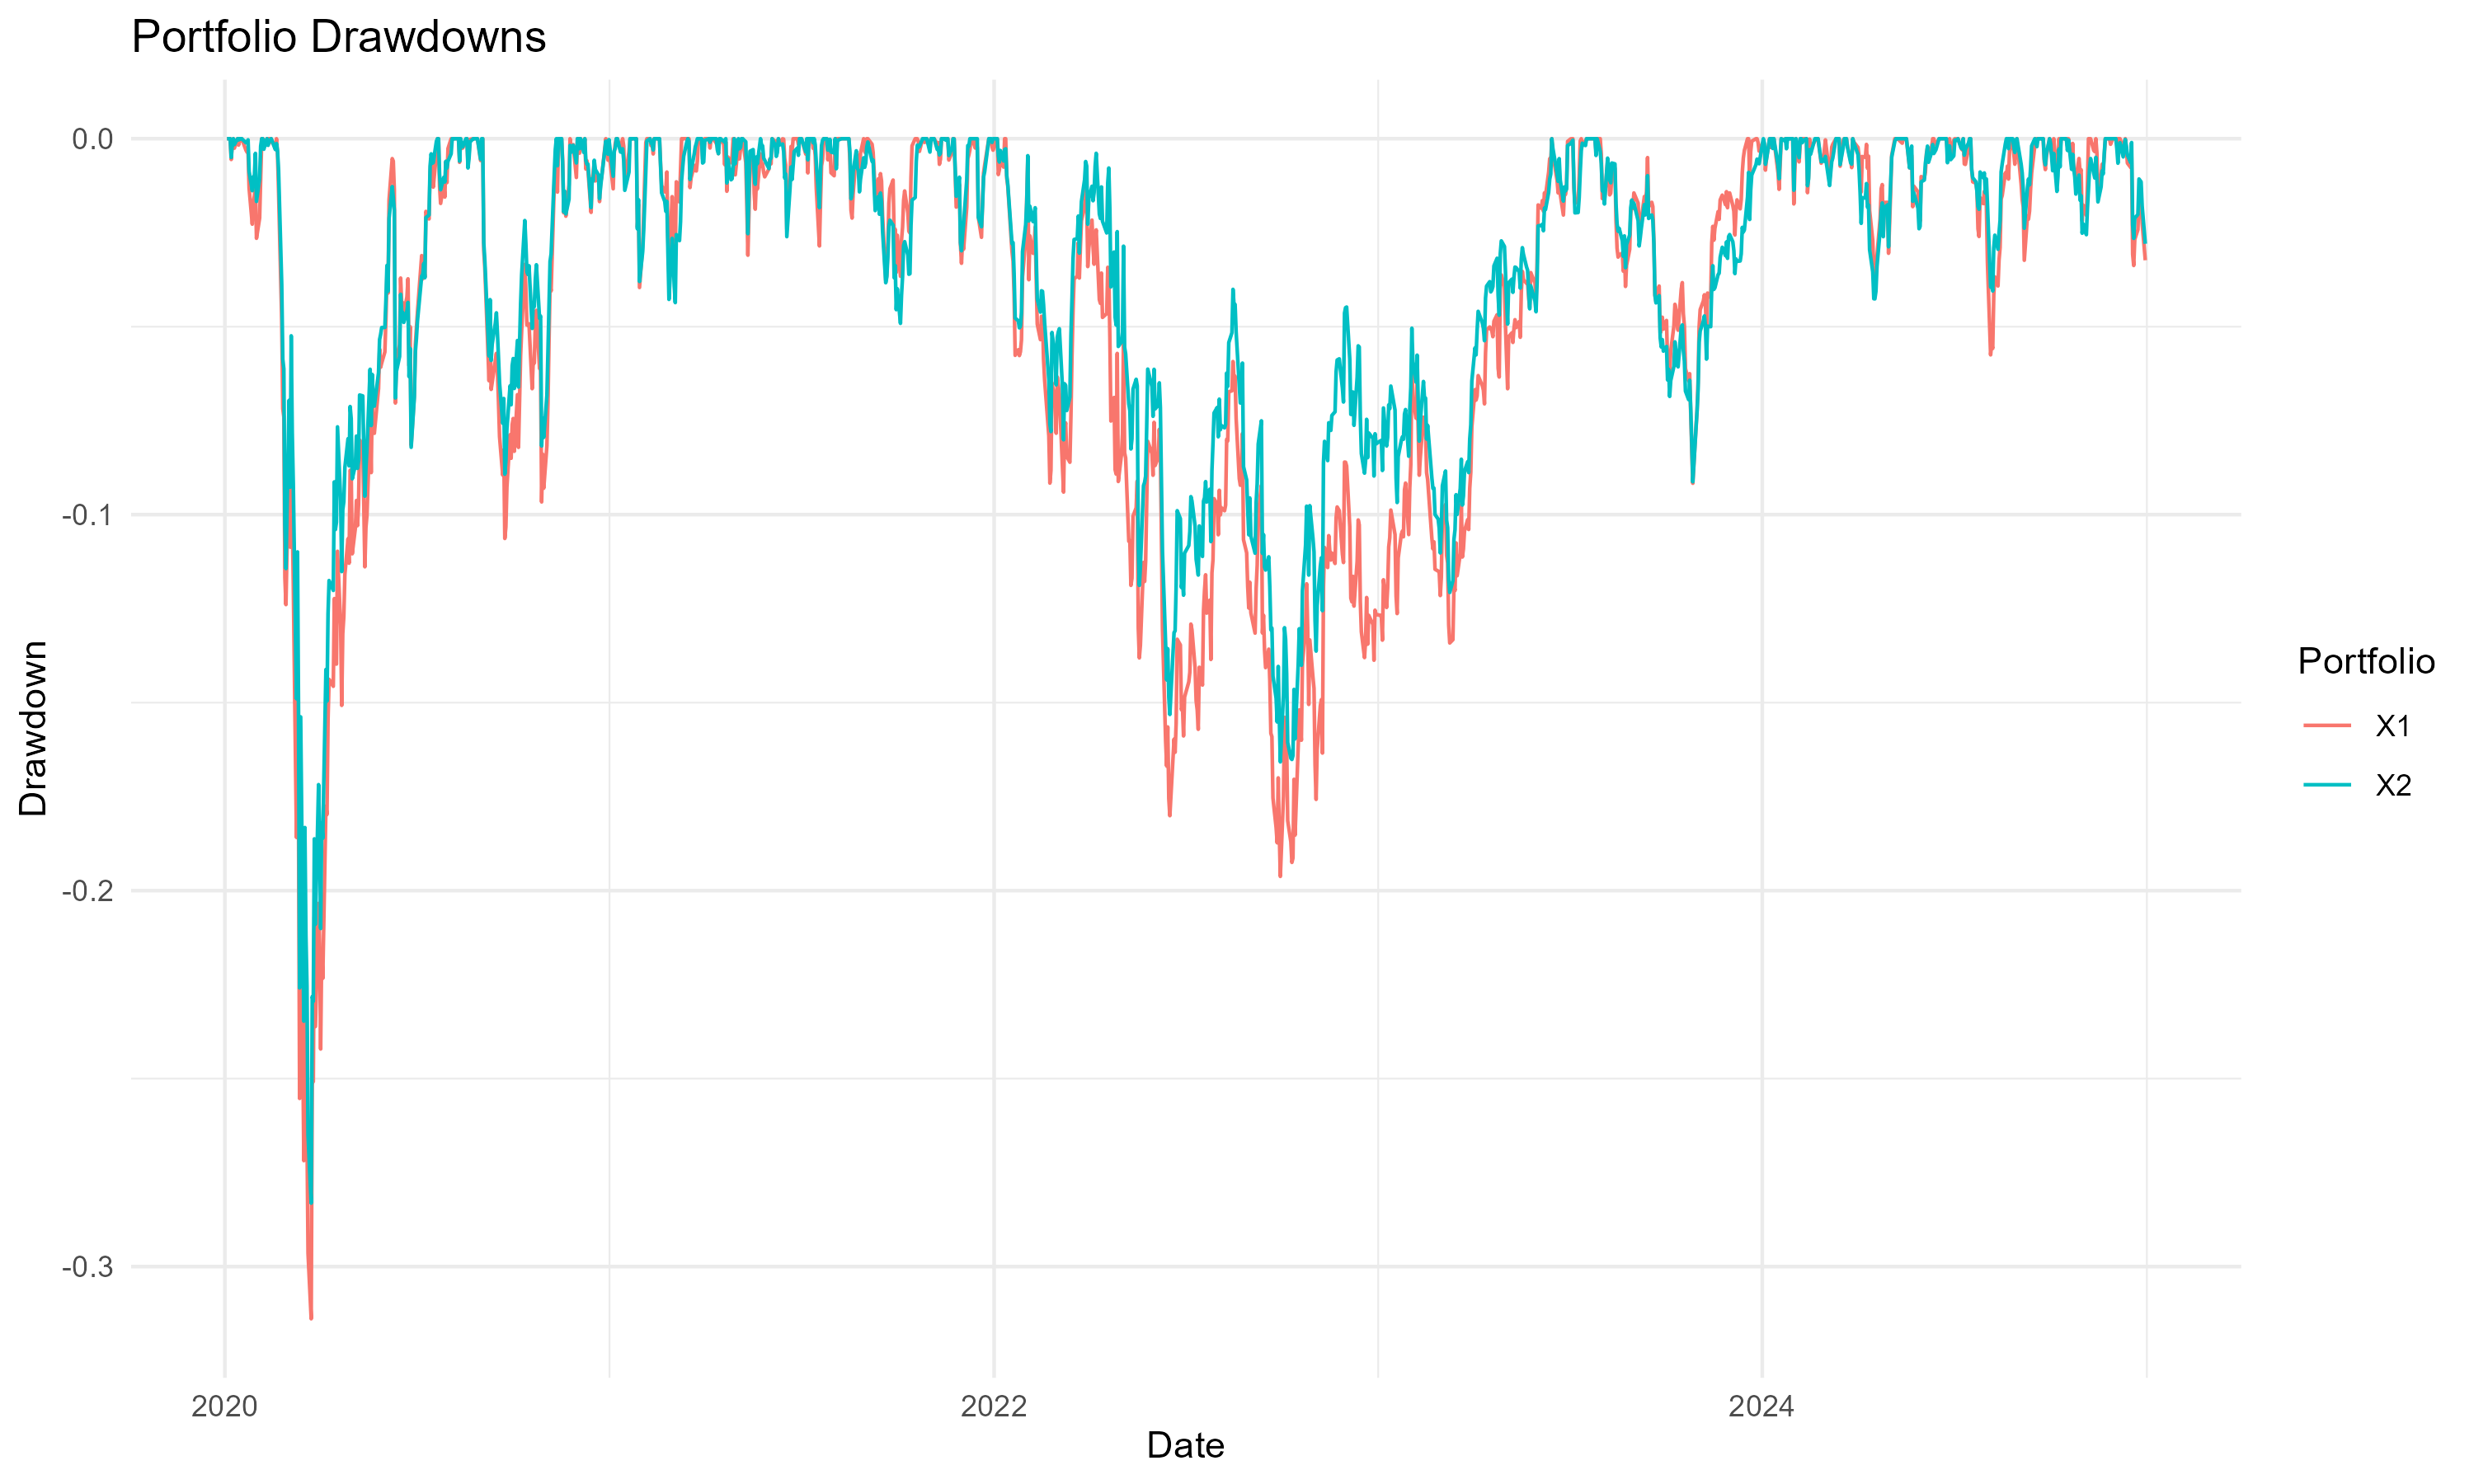
\includegraphics[keepaspectratio]{1-quantitative-finance/../notebooks-and-scripts/1-quantitative-finance/2-unsupervised-learning-for-asset-allocation/r/1-unsupervised-learning-for-asset-allocation-figures/portfolio-drawdowns.png}}

}

\caption{\label{fig-portfolio-drawdowns}Portfolio drawdowns over the
evaluation period, comparing the magnitude and persistence of temporary
losses across the portfolio strategies.}

\end{figure}%

The final performance summary is presented in
Table~\ref{tbl-portfolio-performance}.

\begin{longtable}[]{@{}
  >{\centering\arraybackslash}p{(\linewidth - 8\tabcolsep) * \real{0.2553}}
  >{\centering\arraybackslash}p{(\linewidth - 8\tabcolsep) * \real{0.1915}}
  >{\centering\arraybackslash}p{(\linewidth - 8\tabcolsep) * \real{0.2340}}
  >{\centering\arraybackslash}p{(\linewidth - 8\tabcolsep) * \real{0.1383}}
  >{\centering\arraybackslash}p{(\linewidth - 8\tabcolsep) * \real{0.1809}}@{}}
\caption{Performance comparison between the Hierarchical Risk Parity
(HRP) portfolio and the equal-weight benchmark portfolio.
}\label{tbl-portfolio-performance}\tabularnewline
\toprule\noalign{}
\begin{minipage}[b]{\linewidth}\centering
Portfolio
\end{minipage} & \begin{minipage}[b]{\linewidth}\centering
Annualized Return
\end{minipage} & \begin{minipage}[b]{\linewidth}\centering
Annualized Volatility
\end{minipage} & \begin{minipage}[b]{\linewidth}\centering
Sharpe Ratio
\end{minipage} & \begin{minipage}[b]{\linewidth}\centering
Maximum Drawdown
\end{minipage} \\
\midrule\noalign{}
\endfirsthead
\toprule\noalign{}
\begin{minipage}[b]{\linewidth}\centering
Portfolio
\end{minipage} & \begin{minipage}[b]{\linewidth}\centering
Annualized Return
\end{minipage} & \begin{minipage}[b]{\linewidth}\centering
Annualized Volatility
\end{minipage} & \begin{minipage}[b]{\linewidth}\centering
Sharpe Ratio
\end{minipage} & \begin{minipage}[b]{\linewidth}\centering
Maximum Drawdown
\end{minipage} \\
\midrule\noalign{}
\endhead
\bottomrule\noalign{}
\endlastfoot
HRP Portfolio & 0.1754 & 0.2021 & 0.8680 & -0.3139 \\
Equal Weight Portfolio & 0.1514 & 0.1808 & 0.8373 & -0.2831 \\
\end{longtable}

The HRP portfolio achieved a modest improvement in annualized return and
Sharpe ratio relative to the equal-weight benchmark. However, this
improvement was accompanied by a somewhat deeper maximum drawdown during
the evaluation period, illustrating that diversification benefits do not
necessarily translate into lower losses under all market conditions.

The resulting workflow combines PCA, hierarchical clustering, and
risk-based portfolio allocation to study diversification from a
structural rather than purely optimization-based perspective. Rather
than focusing exclusively on return maximization, the analysis
emphasizes robustness, interpretability, and stability under realistic
market conditions.

Additional implementation details, including the companion Quarto and
Python notebooks, are available in the project repository
\href{https://github.com/rodrigokang/portfolio/tree/main/notebooks-and-scripts/1-quantitative-finance/2-unsupervised-learning-for-asset-allocation}{\faGithub}

\section{Results, Discussion, and
Limitations}\label{results-discussion-and-limitations-1}

The results of the analysis suggest that the selected asset universe
exhibits a considerably more structured organization of risk than might
be inferred from asset labels or sector classifications alone. Although
the portfolio contains companies operating across multiple industries,
both the PCA decomposition and the hierarchical clustering analysis
indicate that a relatively small number of latent factors account for a
large proportion of observed market variability.

The PCA results provide the clearest evidence of this concentration. The
first principal component alone explains approximately 46\% of total
variance, while the first two components account for roughly 64\%. More
than 80\% of total variance is captured by the first five components.
These findings suggest that much of the apparent diversity within the
asset universe is driven by a limited set of common risk sources. From a
portfolio construction perspective, this highlights an important
distinction between holding many assets and achieving genuine
diversification. Increasing the number of securities does not
necessarily increase the number of independent sources of risk.

The principal component loadings further support this interpretation.
The first component exhibits broad exposure across most assets and
behaves consistently with a dominant market factor affecting the
portfolio universe as a whole. Subsequent components reveal more
localized patterns associated with sector-specific behaviour and
relative differences between groups of assets. Together, these results
illustrate how PCA can provide a compact representation of market
structure while helping identify hidden concentrations of risk that may
not be immediately visible in the original return space.

A complementary perspective emerges from the hierarchical clustering
analysis. The dendrogram and clustered correlation matrix reveal
economically intuitive groupings that arise directly from the data.
Technology companies tend to cluster together, energy firms form a
separate branch, and defensive sectors exhibit their own hierarchical
relationships. Rather than imposing predefined classifications, the
clustering procedure allows the statistical organization of the market
to emerge from observed return behaviour. This provides a useful
framework for understanding how diversification is distributed across
the portfolio and where concentrations of risk may exist.

The portfolio construction stage extends these observations into an
allocation framework. Compared with the equal-weight benchmark, the
Hierarchical Risk Parity portfolio produces a noticeably different
allocation structure. The largest weights were assigned to JNJ, KO, PG,
and WMT, while exposure to several technology, financial, and energy
assets was reduced. Importantly, this outcome should not be interpreted
as a prediction that these assets will outperform in the future. Rather,
it reflects their role within the correlation structure of the portfolio
and the objective of distributing risk more evenly across the hierarchy
identified during the clustering stage.

This distinction is central to the interpretation of the results. The
primary contribution of HRP is not necessarily superior return
generation, but a different approach to diversification. Traditional
portfolio construction methods often allocate capital directly, whereas
HRP attempts to allocate risk. As a consequence, two portfolios with
similar levels of capital diversification may exhibit substantially
different risk concentrations. The risk contribution analysis suggests
that the HRP framework achieves a more balanced distribution of
portfolio risk across assets, consistent with its underlying design
objectives.

Performance comparisons between the HRP portfolio and the equal-weight
benchmark reveal both strengths and trade-offs. The HRP portfolio
achieved a modest improvement in annualized return and Sharpe ratio
relative to the benchmark. At the same time, it experienced a somewhat
deeper maximum drawdown during the evaluation period. These results
illustrate an important practical point: improvements in one dimension
of portfolio performance do not necessarily translate into improvements
across all dimensions. Diversification, risk balancing, and return
generation remain competing objectives, and no allocation methodology
can fully eliminate these trade-offs.

The results should therefore be interpreted as evidence that
unsupervised learning techniques can provide useful insights into market
structure and portfolio construction rather than as proof of the
superiority of a particular allocation strategy. The analysis
demonstrates that PCA and hierarchical clustering are capable of
uncovering meaningful relationships within the asset universe and that
these relationships can be incorporated into a systematic allocation
process. Whether this ultimately leads to superior long-term investment
performance remains dependent on market conditions, investment horizons,
transaction costs, and implementation choices.

Several limitations should also be acknowledged. First, the analysis was
conducted using a relatively small universe of fifteen assets. While
sufficient for illustrating the methodology, larger investment universes
may exhibit more complex correlation structures and different clustering
behaviour. Second, the study relies on a single historical sample
period. Financial markets are inherently dynamic, and correlation
structures evolve through time, particularly during periods of economic
stress. Consequently, both PCA decompositions and clustering results may
vary across market regimes.

A further limitation is that the analysis assumes frictionless portfolio
implementation. Transaction costs, taxes, liquidity constraints, and
rebalancing considerations were not incorporated into the evaluation. In
practice, these factors can materially influence realized portfolio
performance and may reduce some of the theoretical benefits of more
sophisticated allocation methodologies.

Finally, although HRP was designed to improve robustness relative to
covariance-sensitive optimization frameworks, it does not eliminate
market risk or guarantee protection during severe market downturns.
Common risk factors can still dominate portfolio behaviour when
correlations rise across the market, reducing the effectiveness of
diversification precisely when it is needed most.

Taken together, the results suggest that unsupervised learning
techniques provide a valuable lens through which to study
diversification and market structure. The main contribution of PCA and
HRP in this context is not the pursuit of maximum historical return, but
the ability to make sources of risk more explicit and to organize
portfolio construction around the underlying structure of the market.
From this perspective, the project illustrates how statistical learning
methods can complement traditional portfolio theory by offering a more
interpretable and structurally informed approach to asset allocation.

\section{Technical Appendix
(Optional)}\label{technical-appendix-optional-1}

This appendix provides supplementary mathematical and methodological
details related to the unsupervised learning techniques used throughout
the project. Additional background on PCA and clustering can be found in
\citeproc{ref-james2023statistical}{{[}9{]}} and
\citeproc{ref-hastie2009elements}{{[}15{]}}.

The objective is not to present a comprehensive treatment of the
underlying methods, but rather to summarize the concepts most relevant
to the portfolio construction process. The material presented here
supports the interpretation of the results and clarifies some of the
modeling choices discussed in the main text.

The appendix is organized into two sections. The first summarizes the
principal concepts behind Principal Component Analysis (PCA), which was
used to study the structure of asset return variability and identify
dominant sources of common variation. The second discusses Hierarchical
Clustering (HC), which was used to group assets according to their
similarity patterns and support diversification decisions.

The main body of the project is intended to remain fully understandable
without consulting this appendix. Readers interested primarily in the
practical application and results may safely skip the material that
follows.

\subsection{Principal Component Analysis
(PCA)}\label{principal-component-analysis-pca}

\subsubsection{Centering of Returns}\label{centering-of-returns}

Let

\begin{equation}\phantomsection\label{eq-return-matrix}{
X =
\begin{bmatrix}
r_{11} & r_{12} & \cdots & r_{1p} \\
r_{21} & r_{22} & \cdots & r_{2p} \\
\vdots & \vdots & \ddots & \vdots \\
r_{n1} & r_{n2} & \cdots & r_{np}
\end{bmatrix}
}\end{equation}

denote the matrix of asset returns, where each column corresponds to an
asset and each row represents an observation period.

Prior to applying PCA, the return series were centered by subtracting
the sample mean of each asset:

\begin{equation}\phantomsection\label{eq-centered-returns}{
x_{ij}^{(c)} = r_{ij} - \bar{r}_j
}\end{equation}

where \(\bar{r}_j\) denotes the average return of asset \(j\).

Centering removes differences in mean return levels and ensures that the
subsequent analysis focuses exclusively on the covariance structure of
the data. The centered return matrix was then used to construct the
covariance matrix and perform the eigendecomposition underlying PCA.

\subsubsection{Covariance Matrix}\label{covariance-matrix}

The covariance matrix summarizes the dependence structure among asset
returns and is given by

\begin{equation}\phantomsection\label{eq-covariance-matrix}{
\Sigma = \frac{1}{n-1} X_c^\top X_c
}\end{equation}

where \(X_c\) denotes the centered return matrix and \(n\) is the number
of observations.

Each element \(\sigma_{ij}\) measures the extent to which the returns of
assets \(i\) and \(j\) vary together. Positive values indicate that
returns tend to move in the same direction, whereas negative values
indicate opposite movements.

Because PCA is based on the covariance structure of the data, the matrix
\(\Sigma\) serves as the primary object of analysis. The principal
components are obtained by identifying the directions that explain the
largest share of the variability captured by this matrix.

\subsubsection{Eigenvalue Decomposition}\label{eigenvalue-decomposition}

PCA is based on the eigendecomposition of the covariance matrix,

\begin{equation}\phantomsection\label{eq-eigendecomposition}{
\Sigma = V \Lambda V^\top
}\end{equation}

where \(V\) is the matrix of eigenvectors and \(\Lambda\) is a diagonal
matrix containing the corresponding eigenvalues.

Each eigenvector defines a principal component, while the associated
eigenvalue measures the amount of variance explained by that component.

The principal components are mutually orthogonal and provide a new
coordinate system in which the dominant patterns of variation become
easier to identify. Components associated with larger eigenvalues
explain a greater share of total variance and therefore contain more
information about the structure of asset returns.

In this project, the eigendecomposition of the covariance matrix
provided the basis for evaluating how much of the variability in the
investment universe could be explained by a reduced number of
components.

\subsubsection{Explained Variance}\label{explained-variance}

The eigenvalues obtained from the covariance matrix quantify the amount
of variance explained by each principal component. Let \(\lambda_i\)
denote the eigenvalue associated with the \(i\)-th principal component.
The proportion of variance explained by that component is given by

\begin{equation}\phantomsection\label{eq-pve}{
\text{PVE}_i = \frac{\lambda_i}{\sum_{j=1}^{p}\lambda_j}
}\end{equation}

where \(p\) denotes the total number of assets.

The cumulative proportion of explained variance can be expressed as

\begin{equation}\phantomsection\label{eq-cpve}{
\text{CPVE}_k = \sum_{i=1}^{k} \text{PVE}_i
}\end{equation}

representing the fraction of total variance retained when only the first
\(k\) principal components are considered.

The explained variance analysis indicated a substantial concentration of
variability in a small number of components. The first principal
component accounted for approximately 46\% of total variance, while the
first two components explained roughly 64\%. The first five components
captured more than 80\% of the variability observed across the
investment universe.

These results suggest that a relatively small number of latent factors
drive a large fraction of asset return behavior. Consequently, the
effective dimensionality of the dataset is considerably smaller than the
number of assets included in the analysis.

\subsubsection{Principal Component
Loadings}\label{principal-component-loadings}

While explained variance quantifies the importance of each principal
component, the component loadings describe how individual assets
contribute to those components.

Let

\begin{equation}\phantomsection\label{eq-loading-vector}{
v_k =
\begin{bmatrix}
v_{1k} \\
v_{2k} \\
\vdots \\
v_{pk}
\end{bmatrix}
}\end{equation}

denote the eigenvector associated with the \(k\)-th principal component.
The elements of this vector are commonly referred to as loadings.

Assets with large absolute loadings contribute more strongly to the
corresponding component, whereas assets with loadings closer to zero
have a smaller influence on that source of variation.

The loadings associated with the first two principal components were
examined to identify the assets contributing most strongly to the
dominant patterns of return variability. Because principal components
are linear combinations of the original assets, the loading structure
provides insight into how different securities participate in the latent
factors revealed by the PCA decomposition.

Together with the explained variance analysis, the loadings help
characterize the underlying structure of the investment universe and
identify groups of assets that exhibit similar exposures to common
sources of variation.

\subsubsection{Interpretation for Asset
Allocation}\label{interpretation-for-asset-allocation}

The PCA results indicate that a substantial portion of total variance
can be explained by a relatively small number of principal components.
From a portfolio construction perspective, this suggests that many
assets are influenced by common underlying factors rather than behaving
independently.

As a consequence, the number of securities held in a portfolio may
overstate the true degree of diversification achieved. Assets exposed to
the same dominant components can contribute similar sources of risk even
when they belong to different sectors or industries.

For this reason, PCA can be viewed as a diagnostic tool for assessing
the structure of risk within an investment universe. Rather than
focusing on individual assets, the analysis emphasizes the latent
factors that drive collective movements in returns.

In this project, PCA was used primarily as an exploratory technique to
investigate the dimensionality of the dataset and to identify common
sources of variation prior to the clustering analysis described in the
following section.

\subsection{Hierarchical Clustering
(HC)}\label{hierarchical-clustering-hc}

\subsubsection{Correlation-Based
Distance}\label{correlation-based-distance}

The clustering analysis was based on the correlation structure of asset
returns. Let \(\rho_{ij}\) denote the Pearson correlation coefficient
between assets \(i\) and \(j\). The corresponding distance measure is
defined as

\begin{equation}\phantomsection\label{eq-correlation-distance}{
d_{ij} = \sqrt{\frac{1-\rho_{ij}}{2}}
}\end{equation}

This transformation converts correlations into distances while
preserving the properties required by a distance metric.

Several useful relationships follow directly from this definition:

\begin{itemize}
\tightlist
\item
  If \(\rho_{ij}=1\), then \(d_{ij}=0\).
\item
  If \(\rho_{ij}=0\), then \(d_{ij}=\sqrt{1/2}\).
\item
  If \(\rho_{ij}=-1\), then \(d_{ij}=1\).
\end{itemize}

Assets exhibiting similar return dynamics therefore appear close to one
another in the resulting distance matrix, whereas assets with dissimilar
behavior appear farther apart.

The correlation-based distance matrix served as the primary input to the
hierarchical clustering procedure implemented in this project.

\subsubsection{Agglomerative Clustering}\label{agglomerative-clustering}

Hierarchical clustering was performed using an agglomerative approach.

The procedure begins by assigning each asset to its own cluster. At each
iteration, the two clusters exhibiting the smallest distance are merged
into a new cluster. This process continues until all assets have been
combined into a single hierarchical structure.

If the investment universe contains \(p\) assets, the algorithm
initially creates \(p\) individual clusters. Each merge reduces the
number of clusters by one until the hierarchy is complete.

The resulting sequence of merges reveals how assets are related at
different levels of similarity. Assets that merge early in the process
tend to exhibit highly similar return patterns, whereas assets that
merge only at later stages are generally less related.

\subsubsection{Ward's Linkage Method}\label{wards-linkage-method}

After computing the distance matrix, the clustering algorithm must
determine how distances between clusters are evaluated following each
merge. This choice is known as the linkage criterion.

In this project, Ward's linkage method was employed through the Ward.D2
algorithm.

Ward's method seeks to minimize the increase in within-cluster variance
produced by each merge. At every iteration, the algorithm selects the
pair of clusters whose combination results in the smallest increase in
overall cluster heterogeneity.

This approach tends to generate compact and relatively balanced
clusters, making it particularly useful for identifying coherent groups
of assets exhibiting similar return behavior.

\subsubsection{Dendrogram
Interpretation}\label{dendrogram-interpretation}

The hierarchical structure produced by the clustering algorithm can be
visualized through a dendrogram.

A dendrogram is a tree-like representation that displays the sequence of
cluster merges performed during the agglomerative procedure. Each
terminal node corresponds to an individual asset, while internal nodes
represent cluster combinations formed throughout the algorithm.

The vertical axis represents the distance at which clusters are merged.
Assets connected at lower heights tend to exhibit stronger similarity,
whereas assets that merge only at higher levels are generally less
related.

The dendrogram presented in the main body of the project reveals the
hierarchical organization of the investment universe and highlights
groups of assets exhibiting similar return behavior.

\subsubsection{Clustered Correlation
Matrix}\label{clustered-correlation-matrix}

The ordering produced by hierarchical clustering can be used to
reorganize the correlation matrix according to the cluster structure
identified in the data.

Rather than displaying assets in an arbitrary order, the reordered
matrix places statistically similar assets next to one another. As a
result, groups of highly correlated assets appear as visible blocks
along the diagonal of the matrix.

This representation provides a convenient way to inspect the dependency
structure of the investment universe and to identify groups of assets
sharing similar return dynamics.

In this project, the clustered correlation matrix complemented the
dendrogram by providing an alternative visualization of the
relationships among assets.

\subsection{Diversification Through
Clustering}\label{diversification-through-clustering}

The clustering results indicate that similarities among assets are not
distributed uniformly throughout the investment universe. Instead,
groups of assets exhibiting comparable return behavior emerge naturally
from the data.

From a portfolio construction perspective, these clusters can reveal
hidden concentrations of risk. A portfolio may contain a large number of
securities while remaining exposed to a relatively small set of common
drivers if many holdings belong to the same cluster.

Hierarchical clustering provides a complementary perspective on
diversification by focusing on relationships among assets rather than on
individual securities. Assets belonging to different clusters are more
likely to contribute distinct sources of risk and therefore may improve
portfolio diversification.

Together, PCA and hierarchical clustering provide complementary views of
the structure of asset returns. While PCA identifies dominant sources of
variation, clustering reveals how assets are organized according to
similarity patterns within the investment universe.

\subsubsection{Methodological
Limitations}\label{methodological-limitations}

PCA captures linear relationships among asset returns and may not fully
represent nonlinear dependency structures present in financial markets.

Similarly, the clustering structure obtained depends on both the
distance metric and the linkage criterion employed. Alternative
specifications may produce different cluster configurations and lead to
different interpretations of the investment universe.

Despite these limitations, PCA and hierarchical clustering remain useful
exploratory tools for understanding the structure of asset returns and
supporting diversification analysis.

\chapter{Option Pricing with Path
Integrals}\label{option-pricing-with-path-integrals}

Most option pricing models focus on the value of a contract at maturity.
Path integral methods approach the same problem from a different
perspective: instead of analysing a single outcome, they evaluate the
contribution of all possible price trajectories that could lead to it.
This viewpoint is particularly appealing for derivatives whose value
depends not only on the final price of the underlying asset, but also on
the path followed to reach it.

While the Black--Scholes framework remains one of the most influential
models in quantitative finance, many derivatives require numerical
techniques because closed-form solutions are either unavailable or
difficult to obtain. Path integral methods provide an alternative
formulation that naturally expresses option values as weighted averages
over entire trajectories, creating a direct connection between option
pricing and simulation-based methods.

This project investigates whether a path integral formulation can serve
as a practical computational framework for option pricing. The analysis
focuses on European call options, where analytical Black--Scholes prices
are available and can be used as a benchmark. A path integral
representation of the pricing problem is derived, implemented
numerically using the Metropolis--Hastings algorithm, and evaluated
against both the analytical Black--Scholes solution and conventional
Monte Carlo estimates. Historical market data is incorporated to
illustrate how the methodology can be applied in a realistic setting.

\section{Problem Definition}\label{problem-definition-2}

For a standard European option, the Black--Scholes model provides an
elegant closed-form solution under a set of simplifying assumptions. The
situation becomes more challenging when dealing with contracts that
involve early exercise features, path dependence, or more complex market
dynamics. In these cases, analytical solutions may no longer exist, and
numerical methods become essential.

Most numerical approaches are built around either solving a pricing
equation or approximating the evolution of the underlying asset through
discrete structures such as lattices. Path integral methods offer a
different perspective. Rather than focusing on a single terminal
outcome, they formulate the valuation problem as an aggregation over all
possible trajectories that the underlying asset could follow between the
present and maturity.

This trajectory-based viewpoint is particularly attractive for
derivatives whose value depends on the history of the underlying asset
rather than on its final price alone. It also provides a natural bridge
between option pricing and simulation-based techniques, allowing the
valuation problem to be reformulated in terms of sampling and
aggregating large ensembles of possible price paths.

The central question explored in this project is whether this
alternative formulation can provide a practical foundation for option
pricing while remaining consistent with established financial theory.
The goal is not to outperform Black--Scholes where an analytical
solution already exists, but to examine whether path integrals can serve
as a flexible framework for pricing problems where closed-form solutions
are no longer available.

\section{Modeling Approach}\label{modeling-approach-2}

The starting point of the model is the same stochastic process used in
the Black--Scholes framework. The underlying asset is assumed to follow
a geometric Brownian motion, allowing the option pricing problem to be
expressed in terms of the probability distribution of future price
trajectories.

Rather than working directly with the Black--Scholes partial
differential equation, the pricing problem is reformulated using a path
integral representation. In this formulation, the value of an option is
obtained by aggregating the contribution of all admissible trajectories
connecting the current asset price to a future state at maturity. Each
trajectory is assigned a statistical weight determined by the underlying
stochastic process and contributes to the expected discounted payoff.

To make the problem computationally tractable, the continuous time
horizon is discretized into a finite number of intervals. This
transforms the original path integral into a multidimensional
integration problem whose dimensionality grows with the number of time
steps used to represent the trajectory. The resulting formulation
provides a numerical approximation of the Black--Scholes propagator
while preserving the probabilistic interpretation of the original model.

Evaluating these multidimensional integrals directly quickly becomes
impractical as the number of dimensions increases. For this reason, the
numerical estimation is performed using Markov Chain Monte Carlo
techniques. Among the available sampling methods, the
Metropolis--Hastings algorithm was selected because it allows
representative trajectories to be generated efficiently from the target
distribution without requiring exhaustive exploration of the integration
domain.

The analysis focuses on European call options, where analytical
Black--Scholes prices are available and can be used as a benchmark. This
provides a controlled setting in which the numerical estimates obtained
from the path integral formulation can be compared against a
well-established analytical solution before considering more complex
derivatives.

The overall modeling strategy combines three components: a geometric
Brownian motion describing the evolution of the underlying asset, a path
integral formulation that expresses option values as weighted averages
over entire price trajectories, and a Markov Chain Monte Carlo algorithm
used to estimate those values numerically.

\section{Methodology and
Implementation}\label{methodology-and-implementation-2}

The objective of this project is not to compete with established option
pricing methods, but to explore how ideas originating from the path
integral formulation can be translated into a practical numerical
workflow. To keep the analysis transparent, the implementation is
organized around two experiments. The first uses a controlled setting in
which the analytical solution is known. The second applies the same
workflow to observed market data.

\subsection{Controlled Experiment}\label{controlled-experiment}

The analysis begins with a European call option under the Black-Scholes
assumptions. The parameters used throughout the baseline experiment are
summarized in Table~\ref{tbl-model-parameters}.

\begin{longtable}[]{@{}cc@{}}
\caption{Model parameters used in the baseline pricing
experiment.}\label{tbl-model-parameters}\tabularnewline
\toprule\noalign{}
Parameter & Value \\
\midrule\noalign{}
\endfirsthead
\toprule\noalign{}
Parameter & Value \\
\midrule\noalign{}
\endhead
\bottomrule\noalign{}
\endlastfoot
Initial Asset Price & 100.0000 \\
Strike Price & 100.0000 \\
Time to Maturity & 1.0000 \\
Risk-Free Rate & 0.0500 \\
Volatility & 0.2000 \\
\end{longtable}

Under these assumptions, the Black-Scholes formula provides an exact
analytical price. This creates a useful benchmark against which
numerical estimators can be evaluated.

Although the path integral formulation is naturally expressed in terms
of entire asset price trajectories, a European call option depends only
on the terminal asset price. For this reason, the implementation does
not attempt to sample complete paths through Markov Chain Monte Carlo.
Instead, the problem is simplified by sampling from the terminal
log-price distribution implied by the risk-neutral geometric Brownian
motion model. This reduction preserves the essential pricing problem
while keeping the numerical implementation manageable.

Simulated price paths are nevertheless generated to illustrate the
stochastic dynamics underlying the model and to provide a visual
representation of the path-based perspective motivating the analysis.

\begin{figure}

\centering{

\pandocbounded{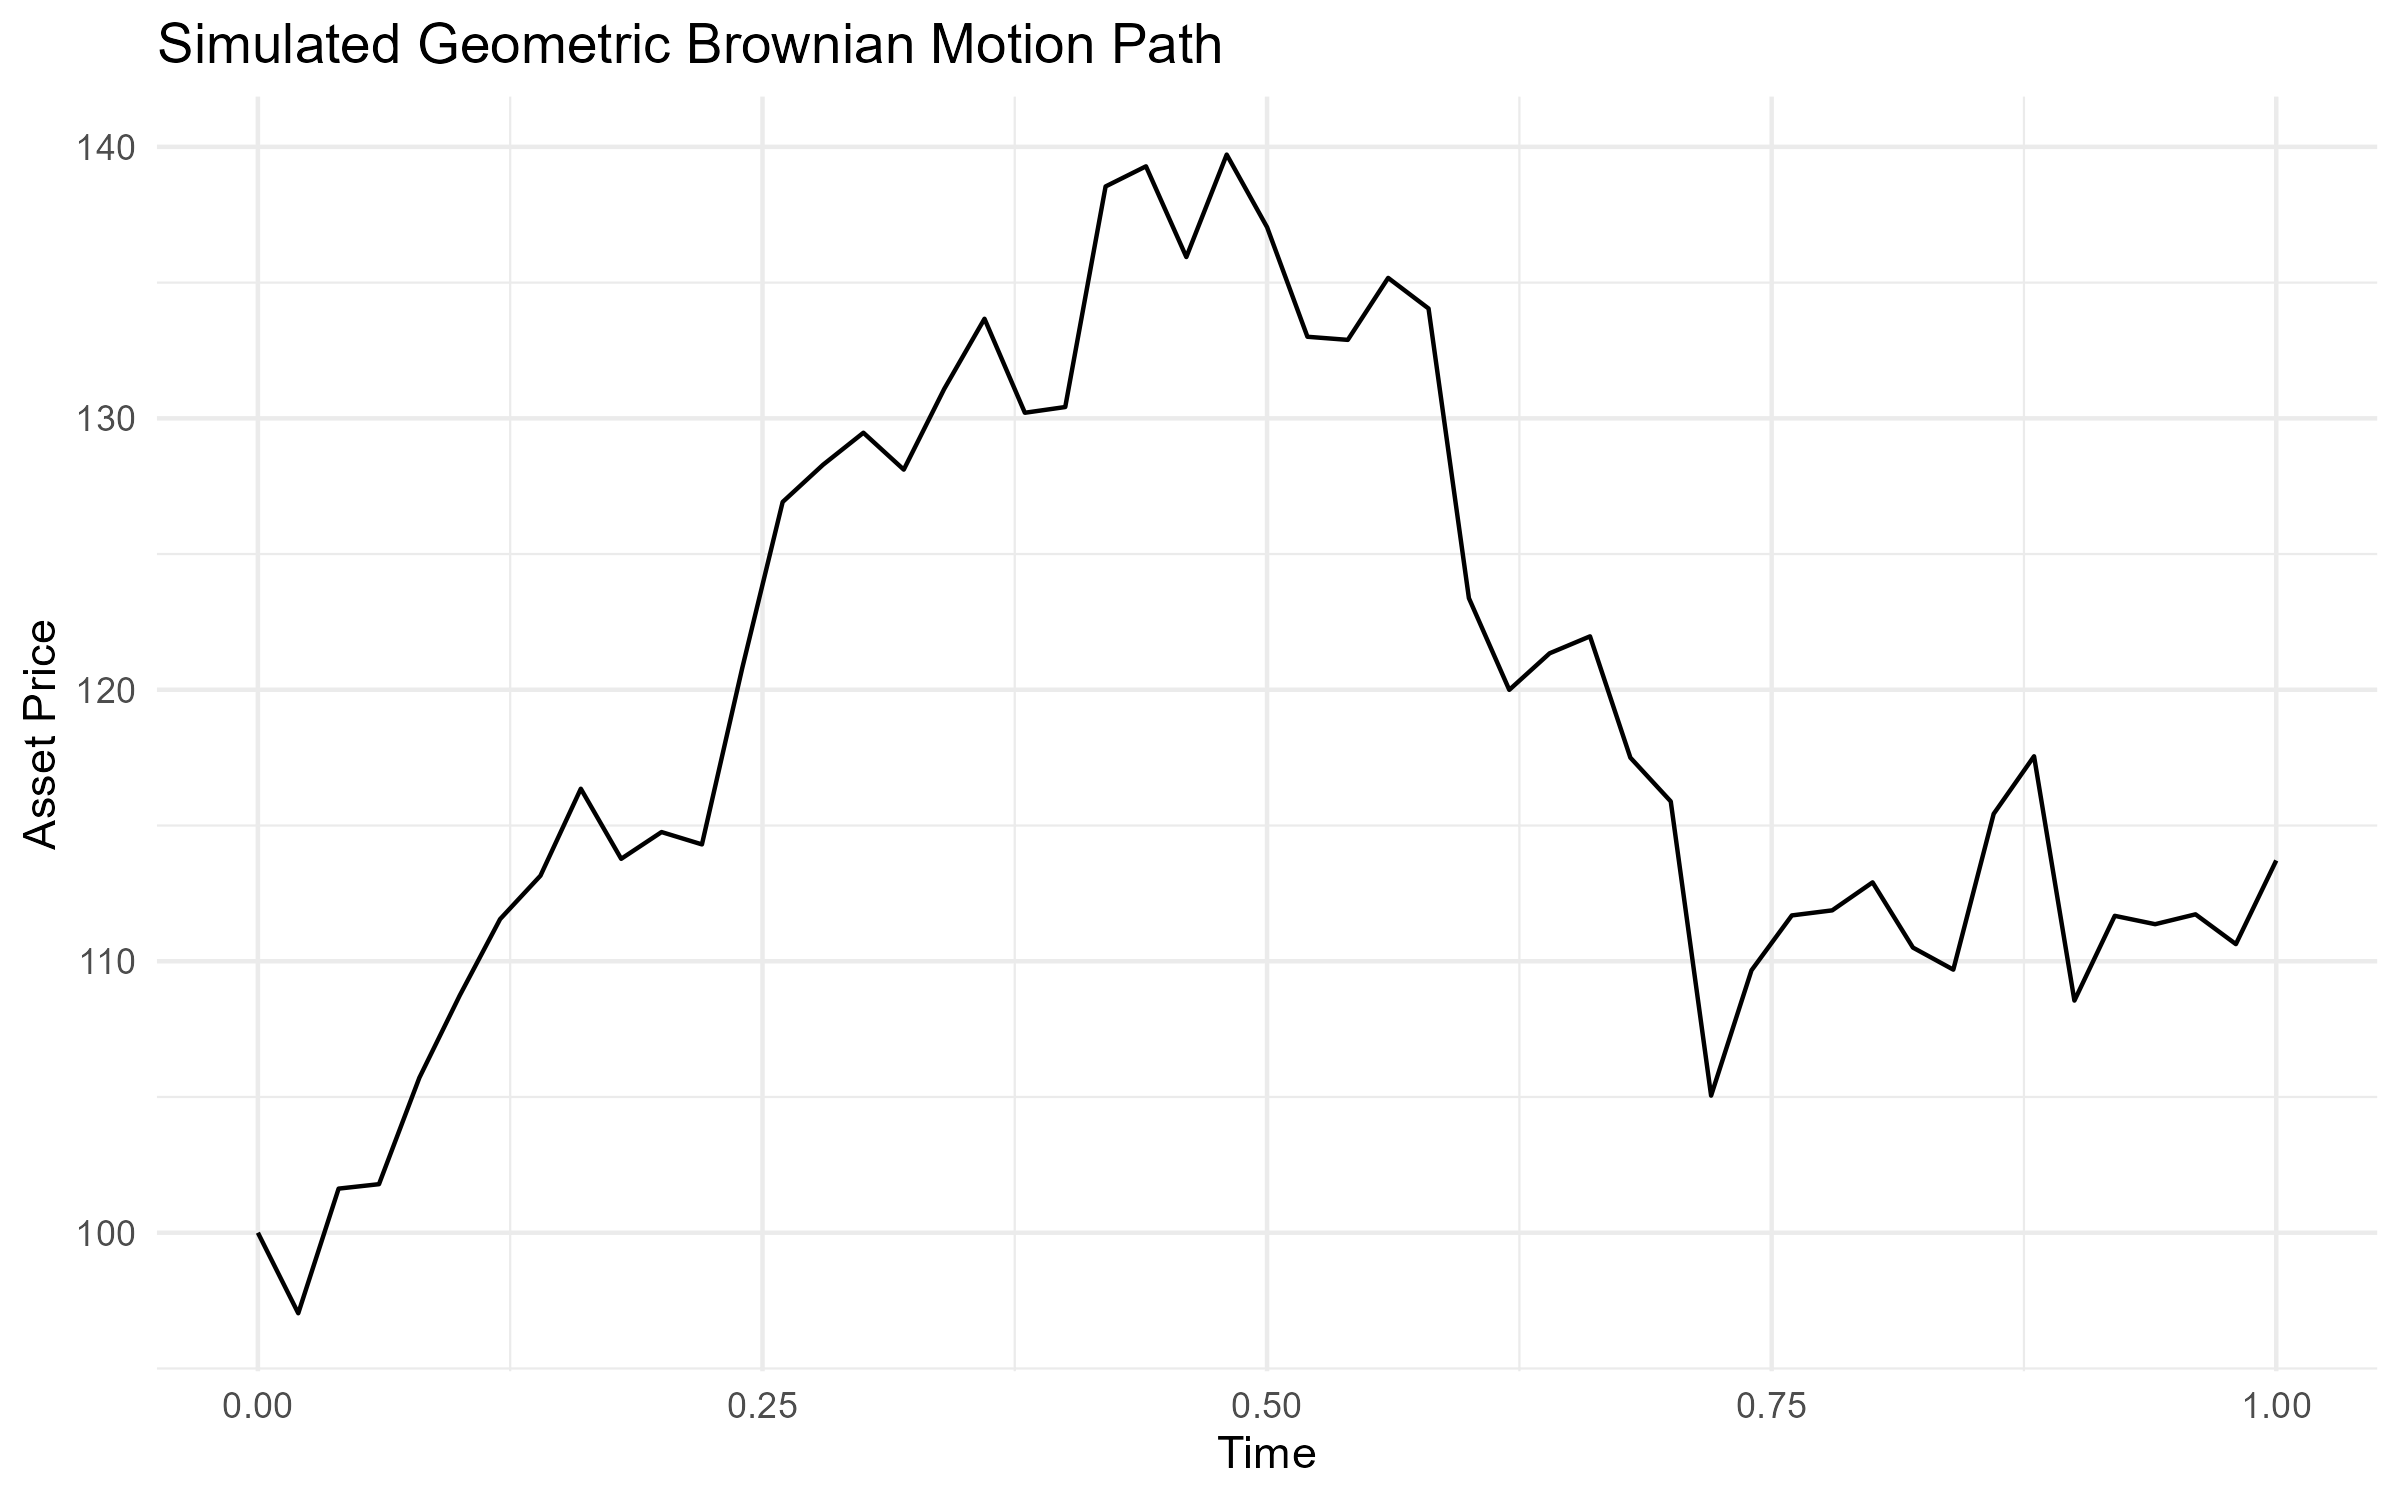
\includegraphics[keepaspectratio]{1-quantitative-finance/../notebooks-and-scripts/1-quantitative-finance/3-option-pricing/r/1-option-pricing-with-path-integrals-figures/simulated-gbm-path.png}}

}

\caption{\label{fig-simulated-gbm-path}A subset of simulated asset-price
trajectories under the risk-neutral geometric Brownian motion model.
Although the final implementation estimates option values from the
terminal distribution, the simulated paths provide a visual
representation of the path-based framework motivating the analysis.}

\end{figure}%

Three pricing approaches are then compared. The Black-Scholes formula
serves as the analytical benchmark, standard Monte Carlo simulation
provides a conventional numerical estimator, and a Metropolis-Hastings
sampler is used to generate samples from the terminal risk-neutral
distribution.

The resulting estimates are reported in Table~\ref{tbl-pricing-methods}
and visualized in Figure~\ref{fig-pricing-method-comparison}.

\begin{longtable}[]{@{}ccc@{}}
\caption{Comparison of option prices obtained using Black-Scholes, Monte
Carlo simulation, and Metropolis-Hastings
sampling.}\label{tbl-pricing-methods}\tabularnewline
\toprule\noalign{}
Method & Option Price & Absolute Error \\
\midrule\noalign{}
\endfirsthead
\toprule\noalign{}
Method & Option Price & Absolute Error \\
\midrule\noalign{}
\endhead
\bottomrule\noalign{}
\endlastfoot
Black-Scholes & 10.4506 & 0.0000 \\
Monte Carlo & 10.3896 & 0.0610 \\
Metropolis-Hastings & 10.5800 & 0.1295 \\
\end{longtable}

\begin{figure}

\centering{

\pandocbounded{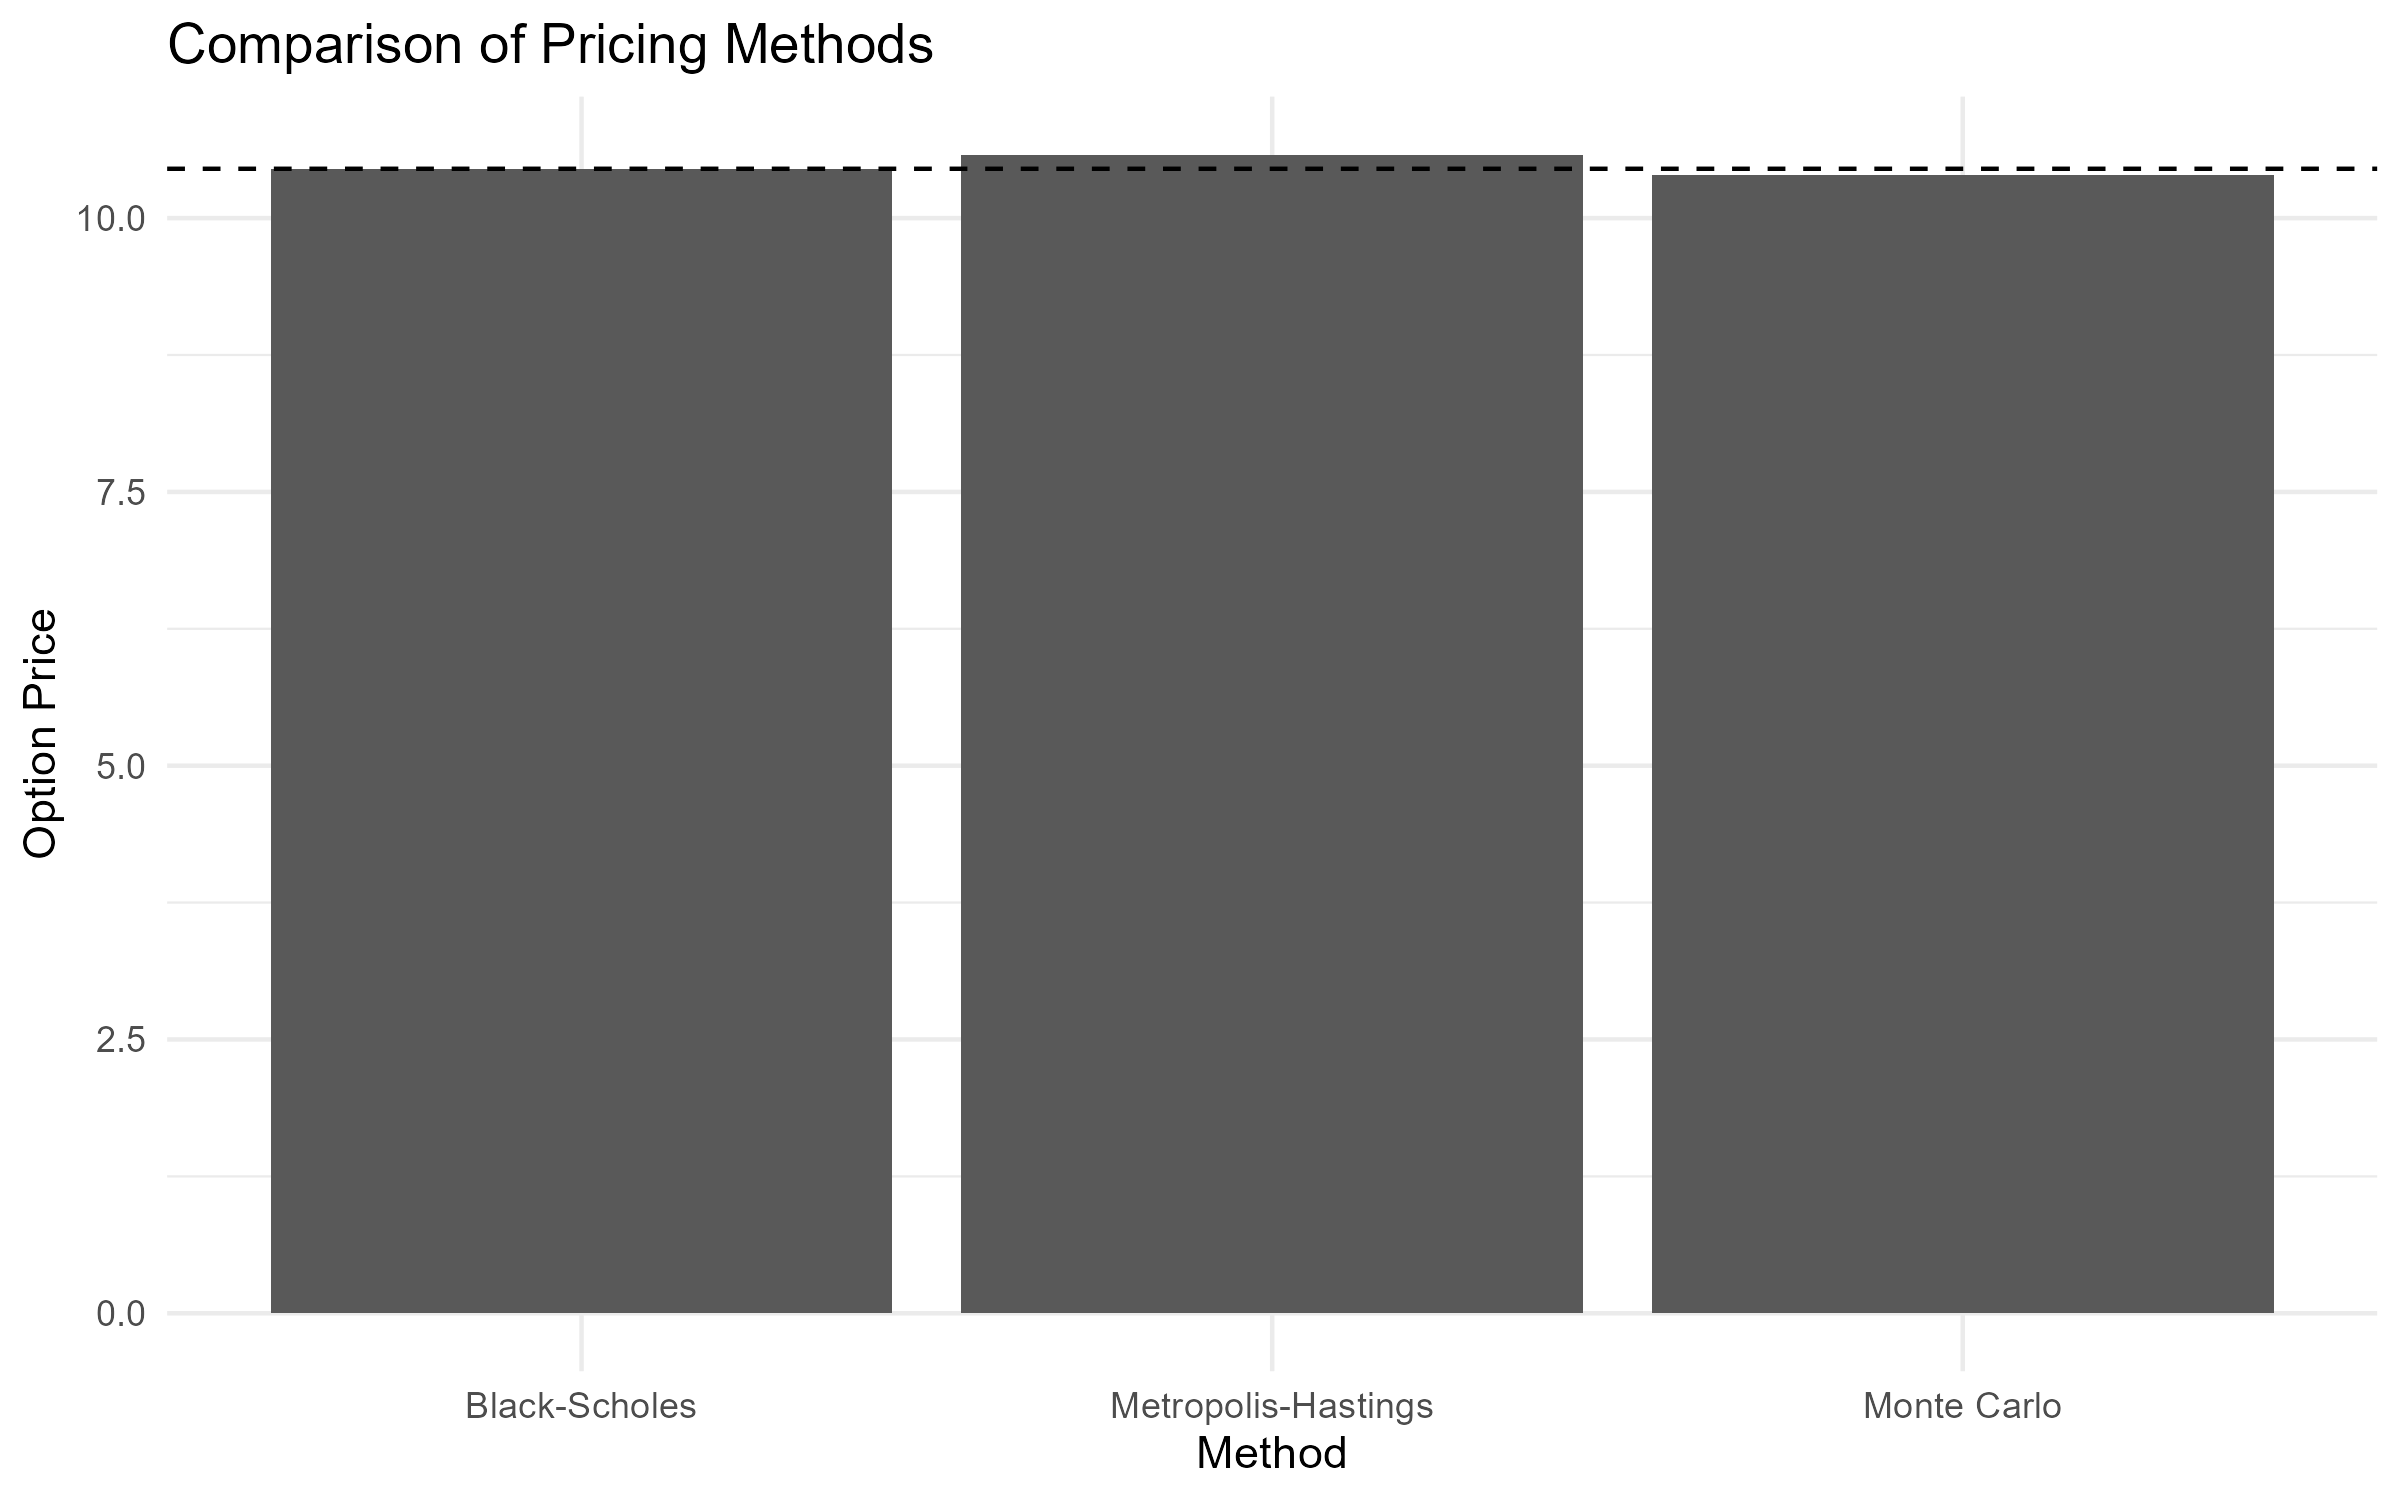
\includegraphics[keepaspectratio]{1-quantitative-finance/../notebooks-and-scripts/1-quantitative-finance/3-option-pricing/r/1-option-pricing-with-path-integrals-figures/pricing-method-comparison.png}}

}

\caption{\label{fig-pricing-method-comparison}Comparison of option
prices obtained using analytical and simulation-based methods.}

\end{figure}%

All three methods produce estimates close to the analytical benchmark.
In this simple setting, standard Monte Carlo achieves the smallest
numerical error. This result is not surprising. For a European call
option, direct Monte Carlo sampling is already an efficient estimator,
and the additional complexity introduced by Markov Chain Monte Carlo
does not provide a clear advantage.

To better understand the behavior of the numerical estimators, the
experiment is repeated for different sample sizes. The results are shown
in Table~\ref{tbl-convergence-analysis} and
Figure~\ref{fig-convergence-analysis}.

\begin{longtable}[]{@{}cccc@{}}
\caption{Convergence behavior of Monte Carlo and Metropolis-Hastings
estimators as the number of samples
increases.}\label{tbl-convergence-analysis}\tabularnewline
\toprule\noalign{}
Samples & Monte Carlo & Metropolis-Hastings & Black-Scholes \\
\midrule\noalign{}
\endfirsthead
\toprule\noalign{}
Samples & Monte Carlo & Metropolis-Hastings & Black-Scholes \\
\midrule\noalign{}
\endhead
\bottomrule\noalign{}
\endlastfoot
100 & 9.2822 & 8.3345 & 10.4506 \\
500 & 11.4302 & 9.4567 & 10.4506 \\
1000 & 10.0559 & 11.6238 & 10.4506 \\
5000 & 10.3909 & 9.8939 & 10.4506 \\
10000 & 10.4008 & 10.8390 & 10.4506 \\
\end{longtable}

\begin{figure}

\centering{

\pandocbounded{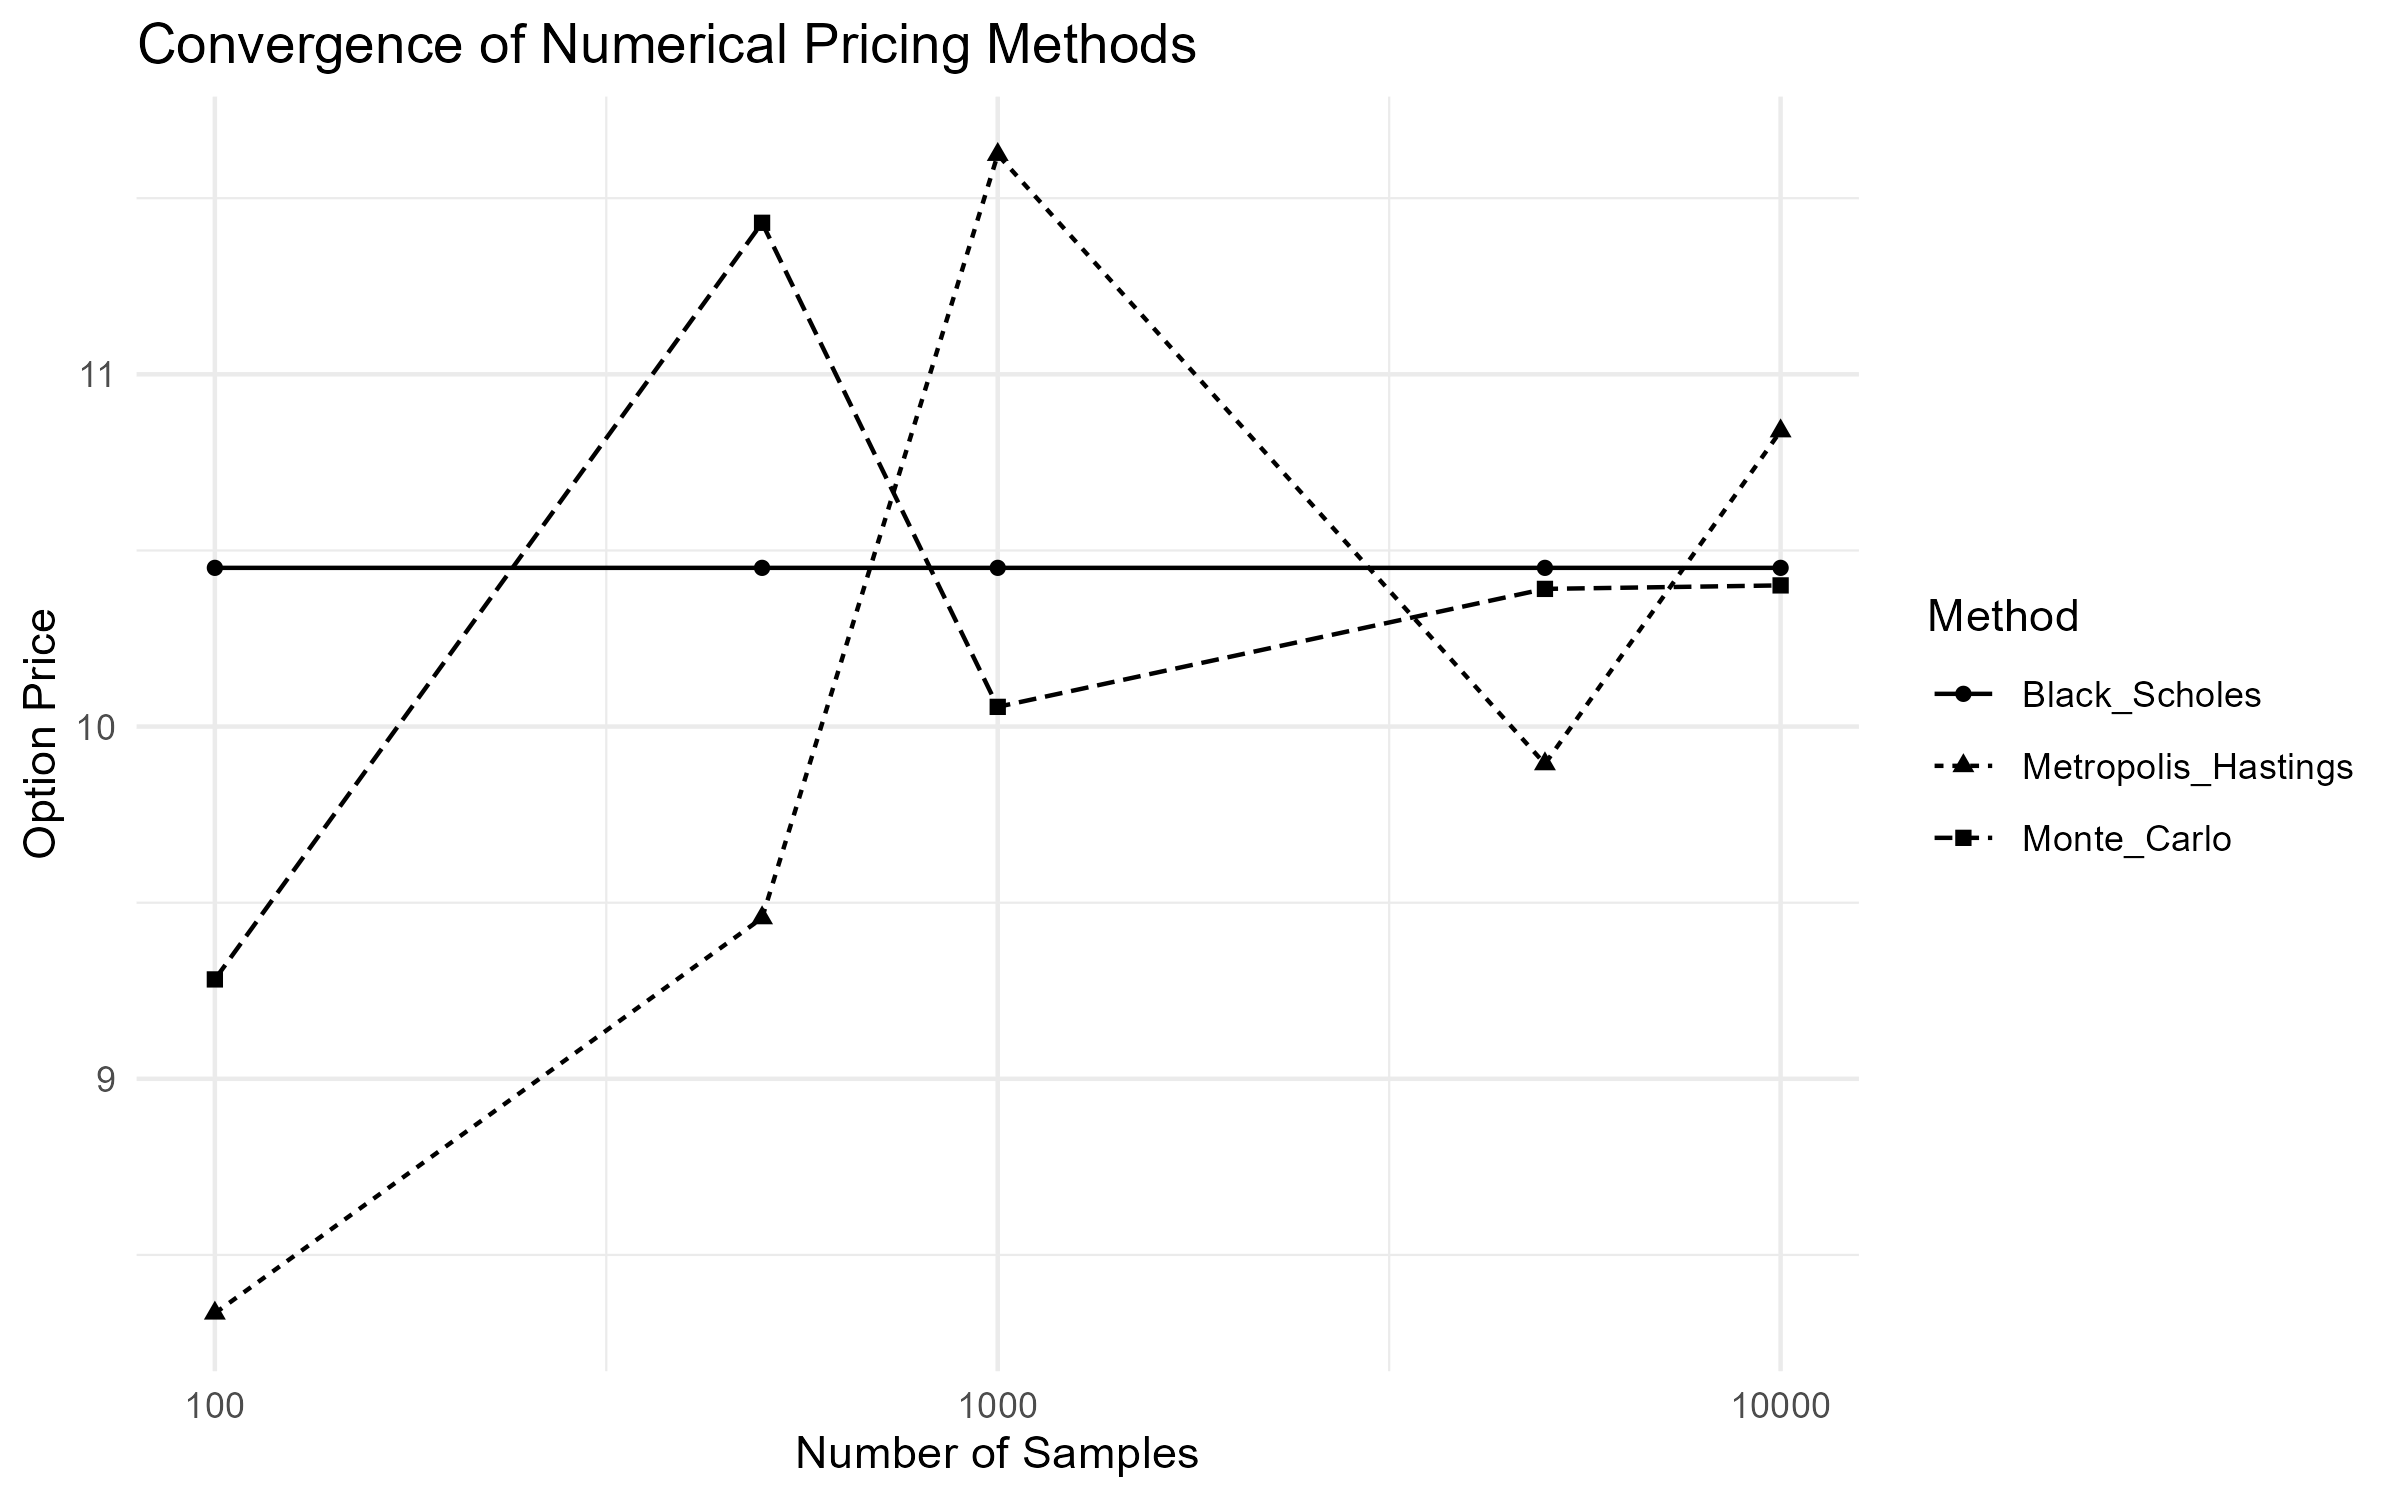
\includegraphics[keepaspectratio]{1-quantitative-finance/../notebooks-and-scripts/1-quantitative-finance/3-option-pricing/r/1-option-pricing-with-path-integrals-figures/convergence-analysis.png}}

}

\caption{\label{fig-convergence-analysis}Convergence of Monte Carlo and
Metropolis-Hastings estimates toward the Black-Scholes benchmark as the
sample size increases.}

\end{figure}%

Both estimators move toward the analytical solution as the sample size
increases. The Monte Carlo estimator exhibits a more stable convergence
pattern, while the Metropolis-Hastings estimates show larger
fluctuations at smaller sample sizes. This behavior is consistent with
the autocorrelation introduced by Markov chain sampling and illustrates
one of the practical trade-offs associated with MCMC-based methods.

The purpose of this comparison is not to demonstrate that
Metropolis-Hastings outperforms Monte Carlo in a problem where the
analytical solution is already available. Rather, it provides a
controlled environment for validating the implementation and
understanding the numerical behavior of the estimator before considering
more complex derivatives.

\subsection{Market Data Example}\label{market-data-example}

After validating the workflow in a controlled setting, the same
methodology is applied using observed market data. Historical prices for
AAPL are downloaded from Yahoo Finance and used to estimate a spot price
and historical volatility.

\begin{figure}

\centering{

\pandocbounded{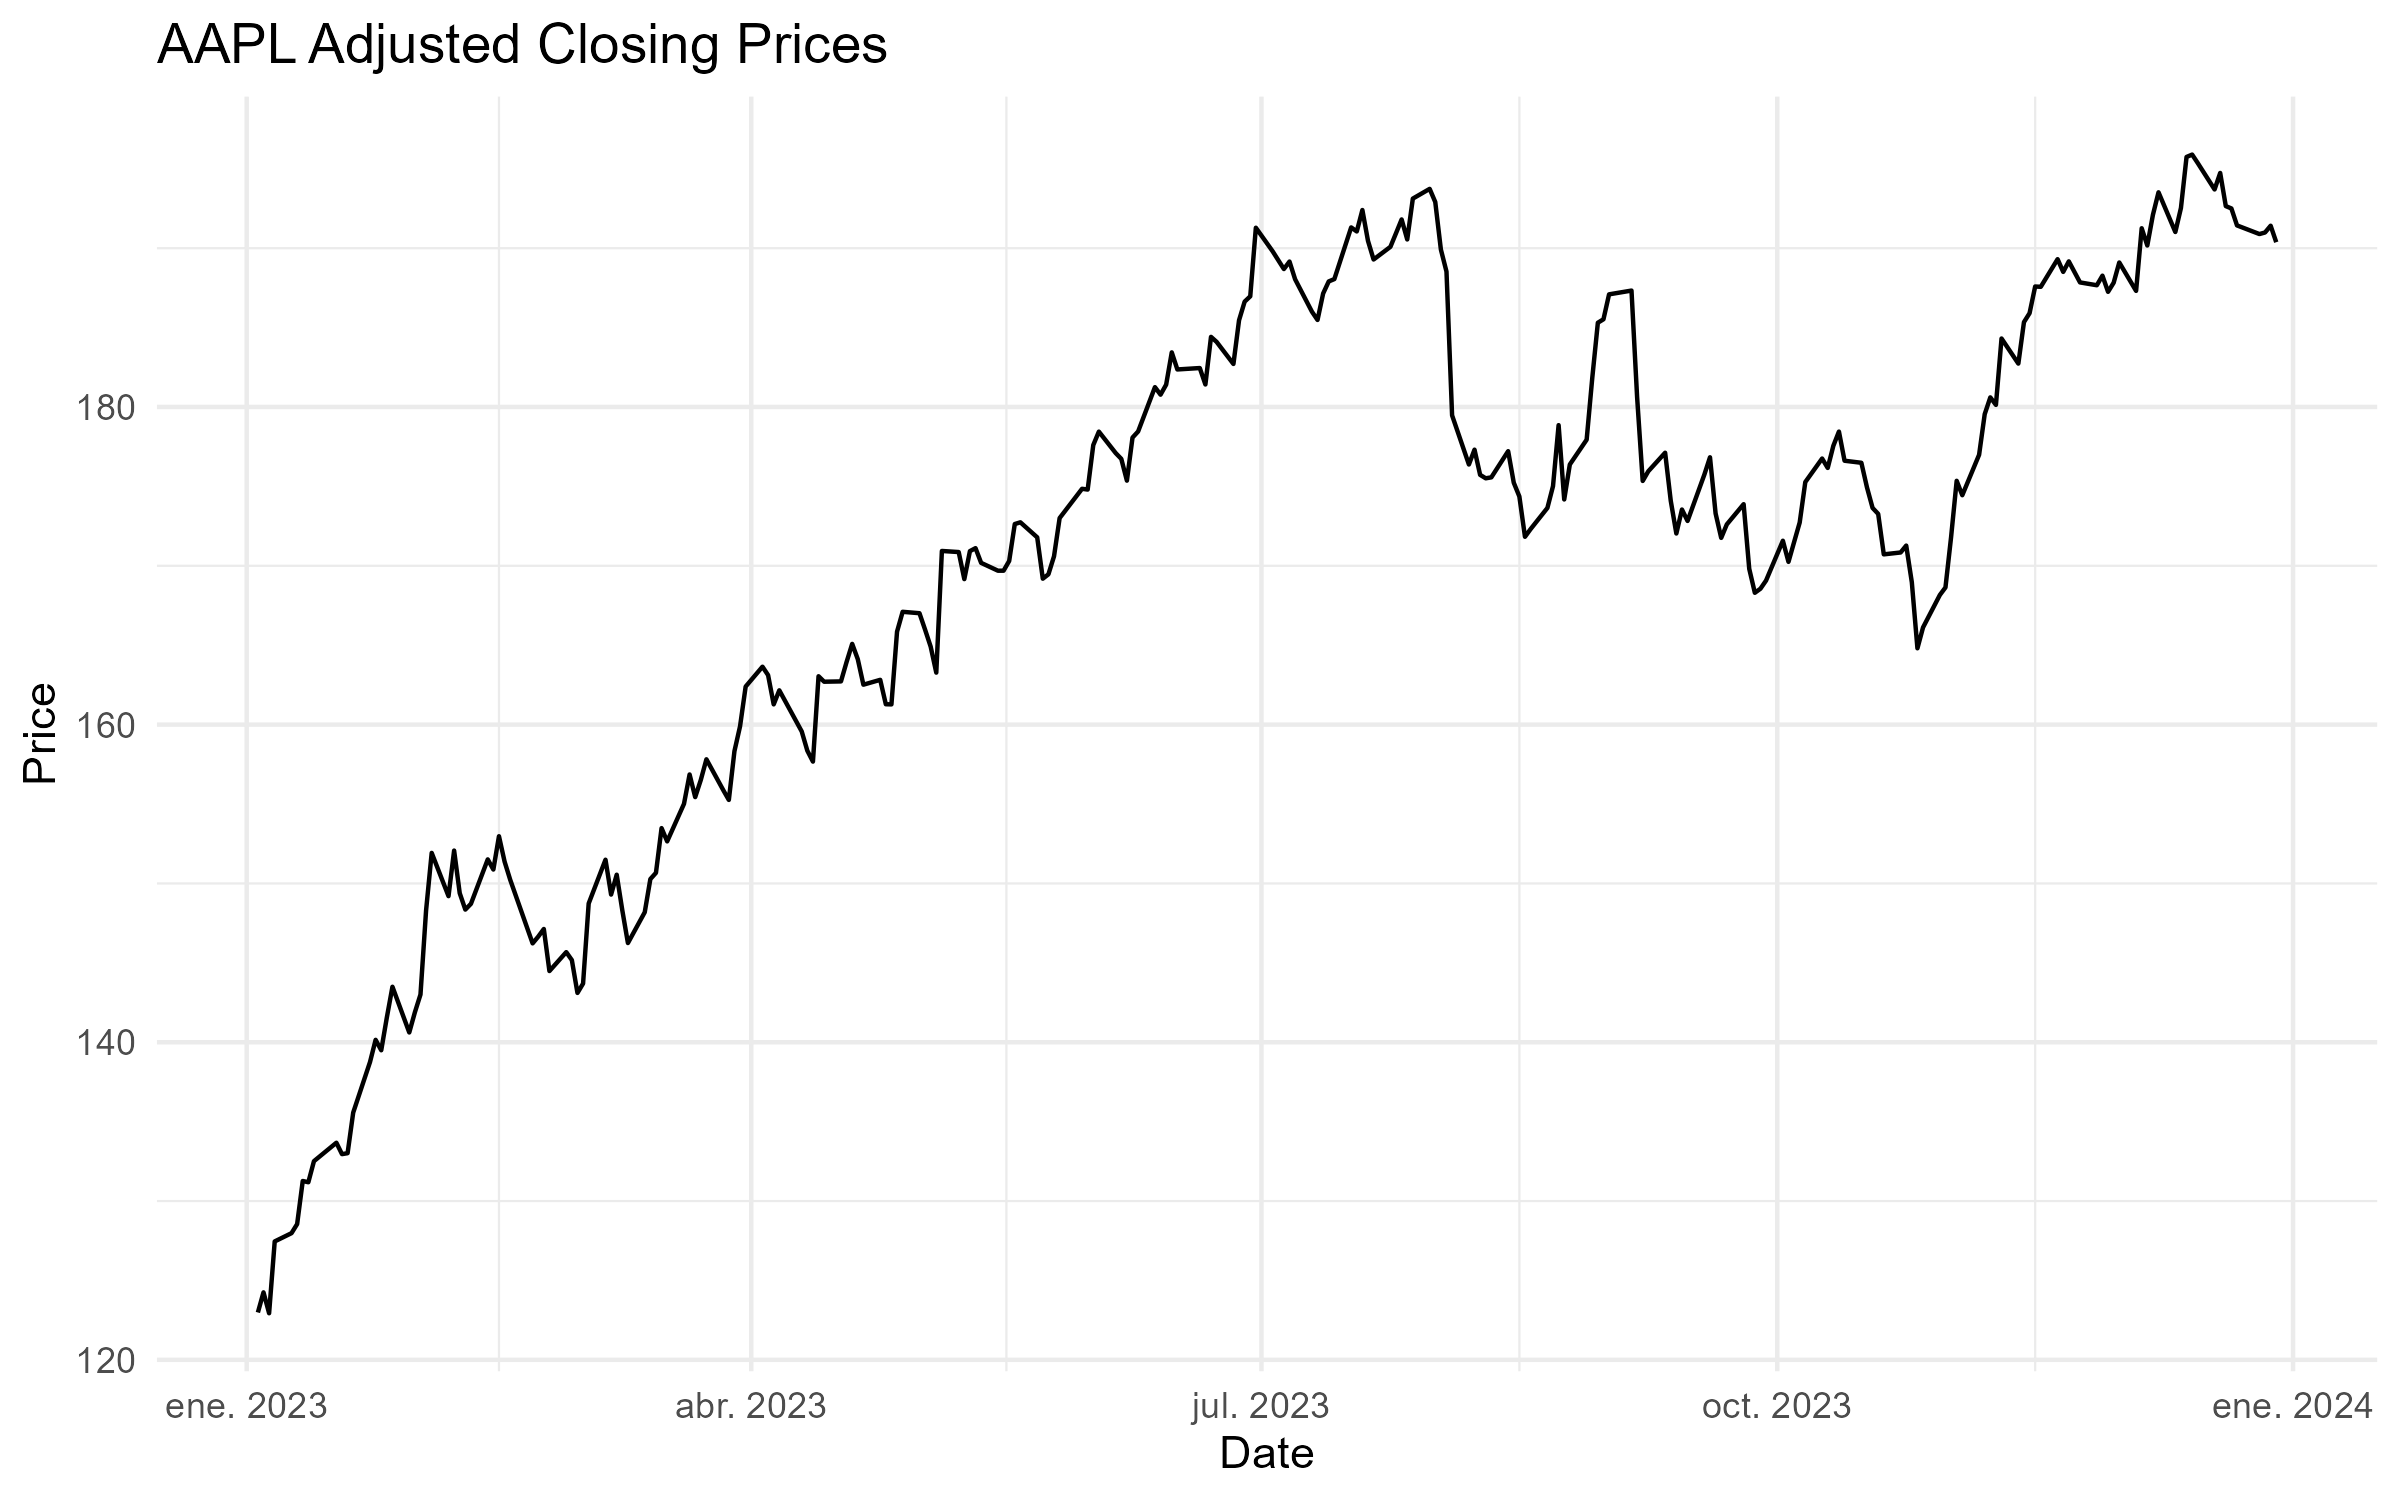
\includegraphics[keepaspectratio]{1-quantitative-finance/../notebooks-and-scripts/1-quantitative-finance/3-option-pricing/r/1-option-pricing-with-path-integrals-figures/market-price-series.png}}

}

\caption{\label{fig-market-price-series}Historical AAPL price series
used in the market-data example.}

\end{figure}%

\begin{figure}

\centering{

\pandocbounded{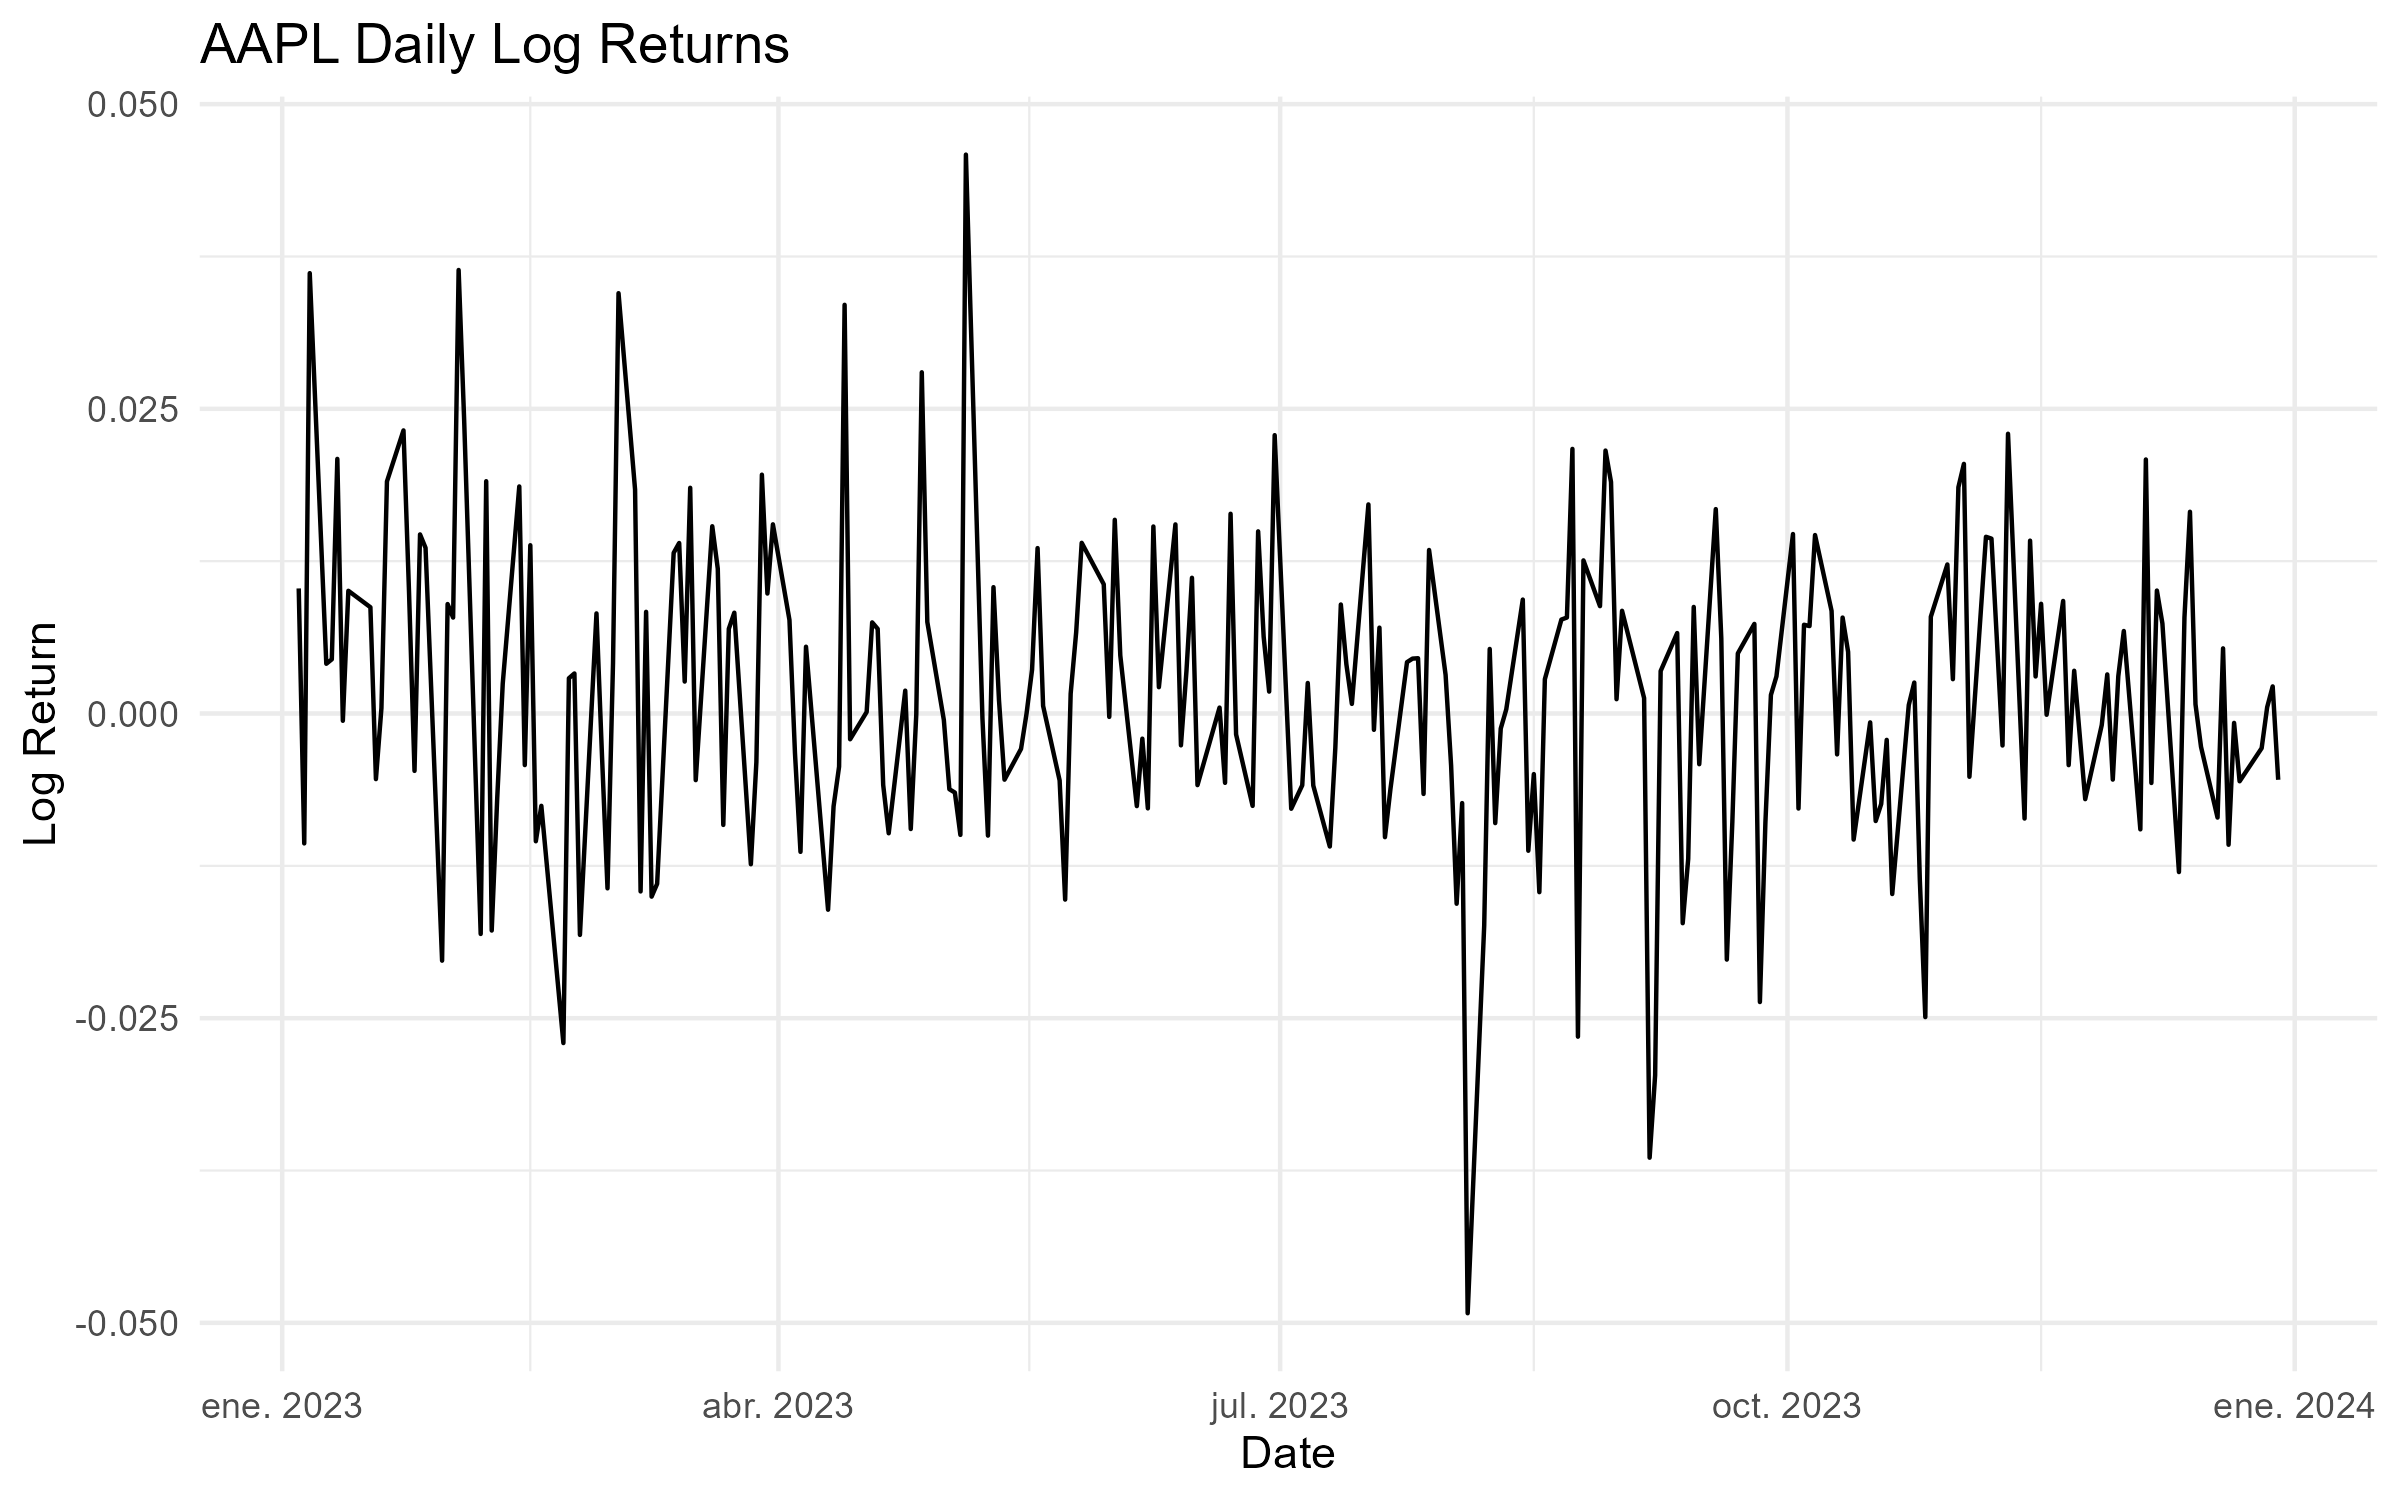
\includegraphics[keepaspectratio]{1-quantitative-finance/../notebooks-and-scripts/1-quantitative-finance/3-option-pricing/r/1-option-pricing-with-path-integrals-figures/market-log-returns.png}}

}

\caption{\label{fig-market-log-returns}Historical log returns used to
estimate the volatility parameter employed in the pricing exercise.}

\end{figure}%

The resulting inputs are summarized in Table~\ref{tbl-market-inputs}.

\begin{longtable}[]{@{}cc@{}}
\caption{Market-derived inputs obtained from historical AAPL
data.}\label{tbl-market-inputs}\tabularnewline
\toprule\noalign{}
Parameter & Value \\
\midrule\noalign{}
\endfirsthead
\toprule\noalign{}
Parameter & Value \\
\midrule\noalign{}
\endhead
\bottomrule\noalign{}
\endlastfoot
Ticker & AAPL \\
Spot Price & 190.3751 \\
Strike Price & 190.3751 \\
Time to Maturity & 1 \\
Risk-Free Rate & 0.05 \\
Historical Volatility & 0.1992 \\
\end{longtable}

The objective of this second experiment is not to construct a tradable
option pricing model or a production-grade calibration. Instead, it
demonstrates that the same workflow can be applied using observed
financial data rather than synthetic inputs.

Pricing results obtained from the three methods are reported in
Table~\ref{tbl-market-comparison} and visualized in
Figure~\ref{fig-market-pricing-comparison}.

\begin{longtable}[]{@{}ccc@{}}
\caption{Option pricing results using market-derived inputs from AAPL
historical data.}\label{tbl-market-comparison}\tabularnewline
\toprule\noalign{}
Method & Option Price & Absolute Error \\
\midrule\noalign{}
\endfirsthead
\toprule\noalign{}
Method & Option Price & Absolute Error \\
\midrule\noalign{}
\endhead
\bottomrule\noalign{}
\endlastfoot
Black-Scholes & 19.8397 & 0.0000 \\
Monte Carlo & 19.6705 & 0.1693 \\
Metropolis-Hastings & 19.5573 & 0.2824 \\
\end{longtable}

\begin{figure}

\centering{

\pandocbounded{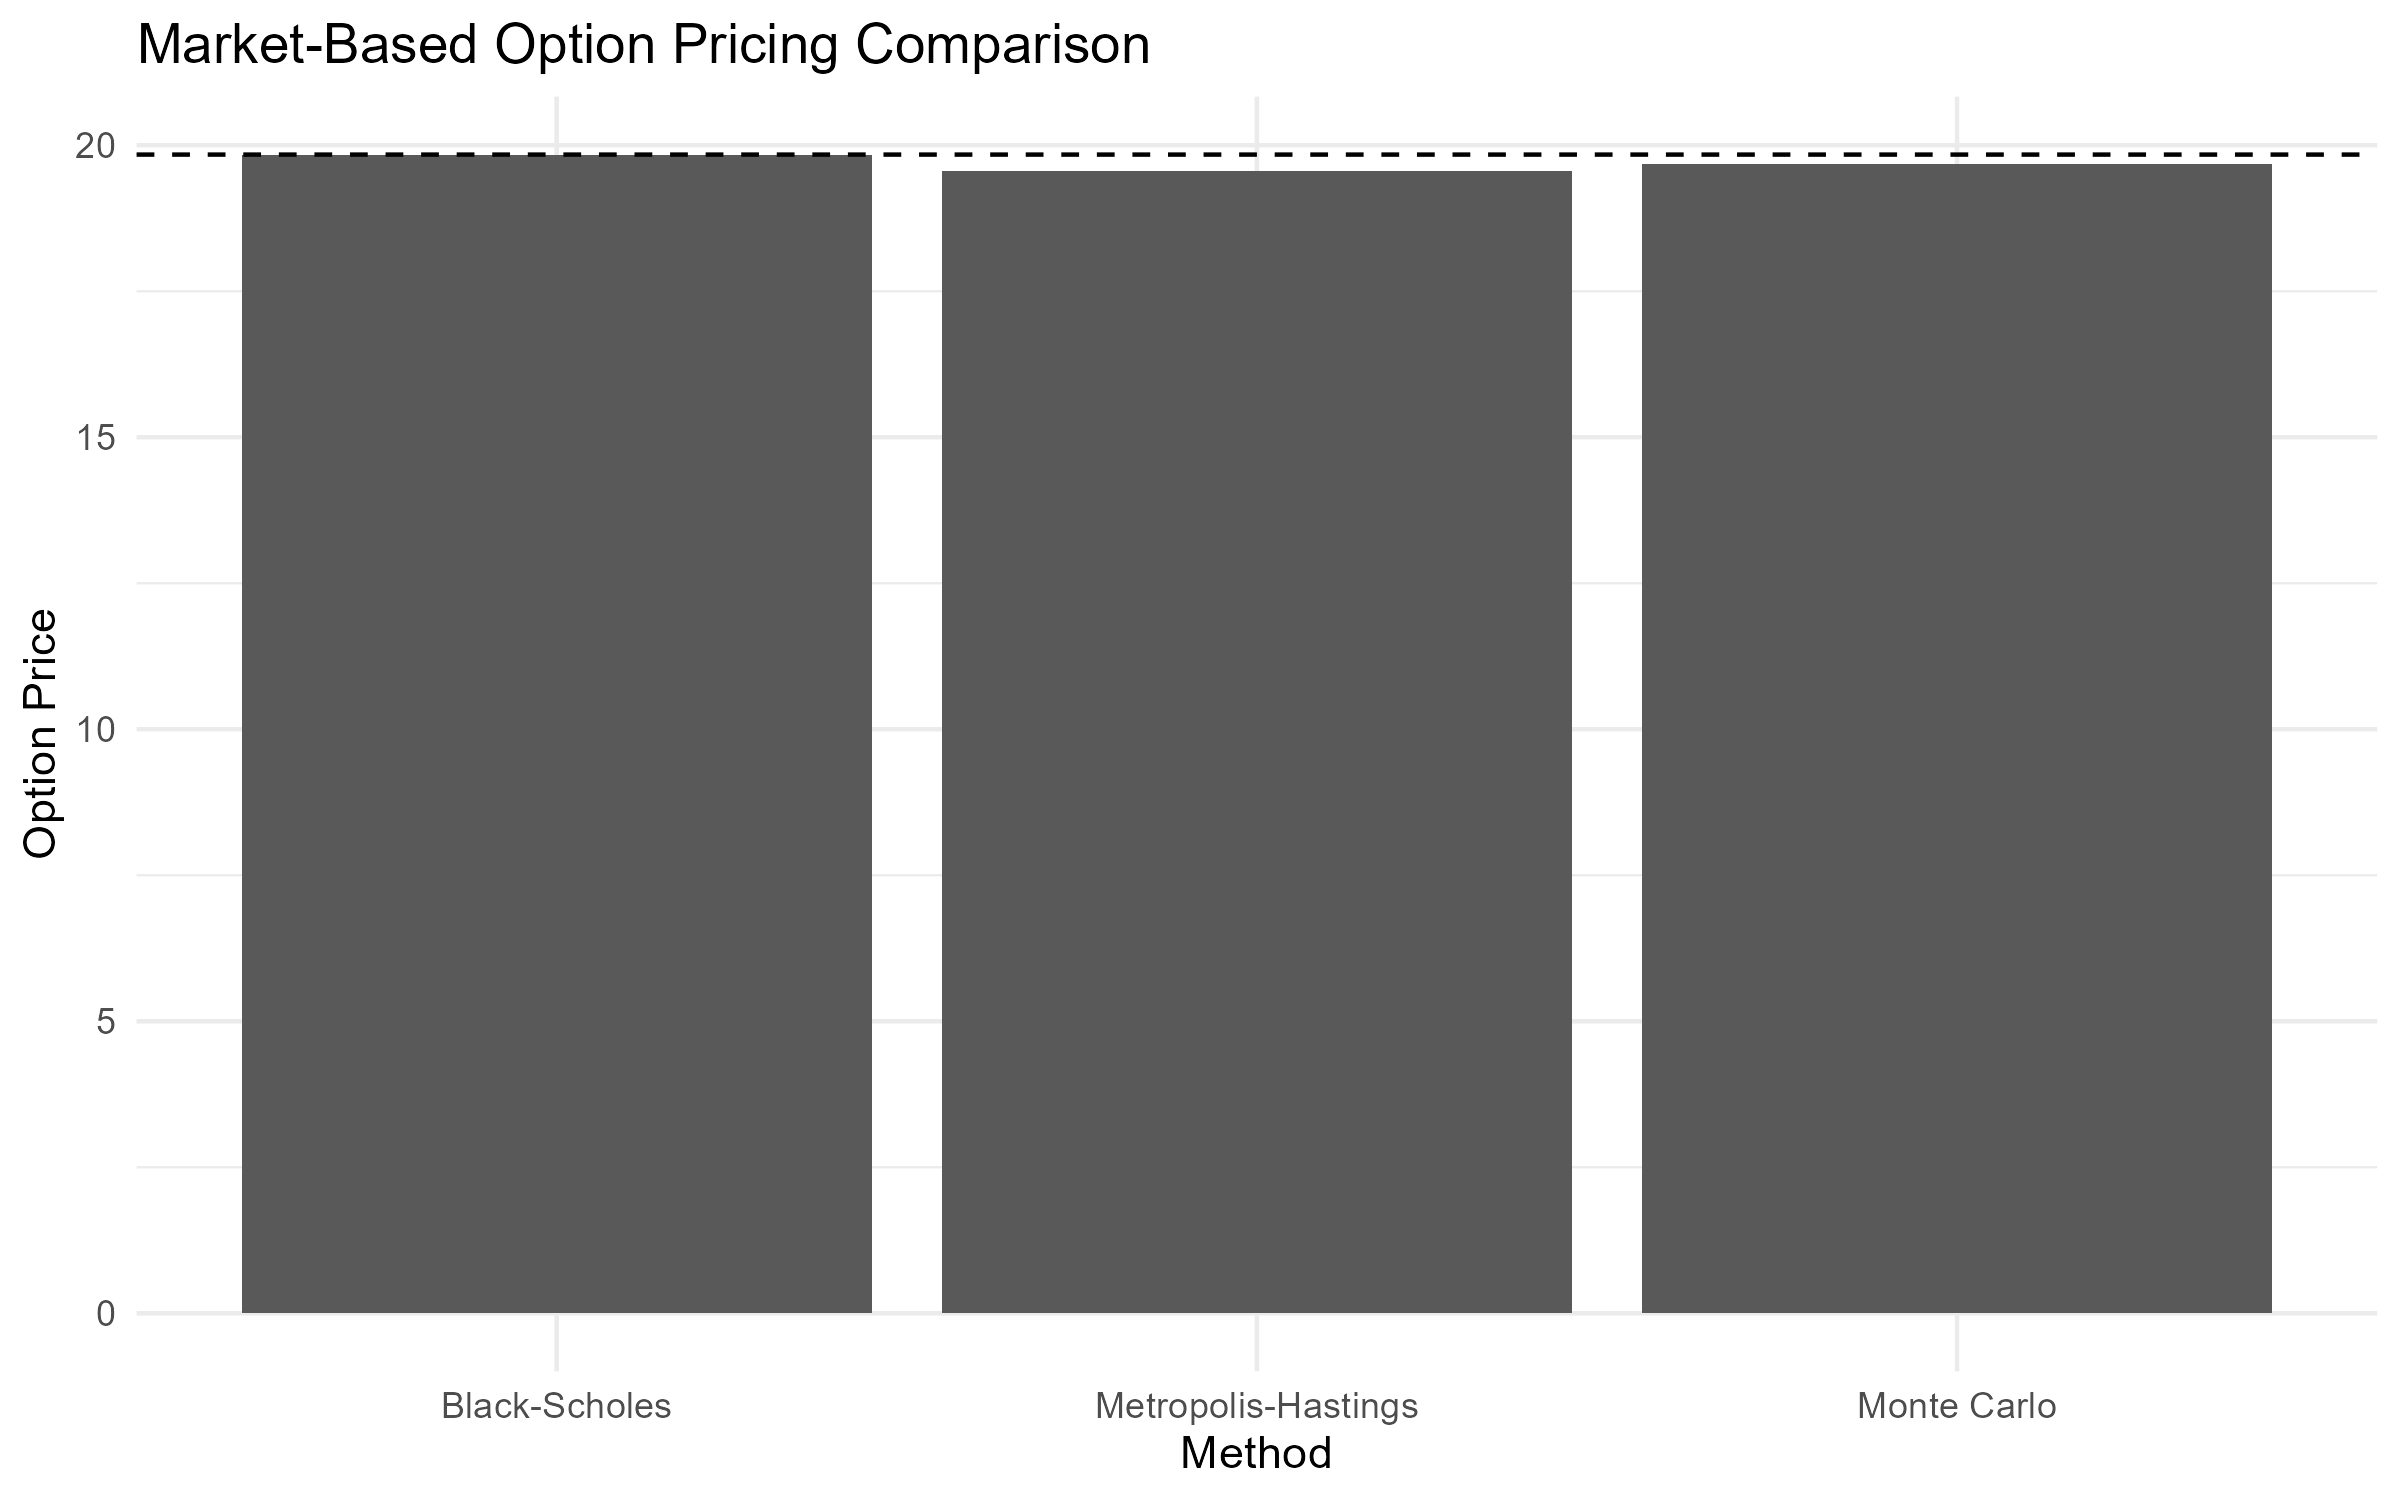
\includegraphics[keepaspectratio]{1-quantitative-finance/../notebooks-and-scripts/1-quantitative-finance/3-option-pricing/r/1-option-pricing-with-path-integrals-figures/market-pricing-comparison.png}}

}

\caption{\label{fig-market-pricing-comparison}Comparison of pricing
estimates obtained using market-derived inputs from AAPL historical
data.}

\end{figure}%

The overall conclusions are consistent with those obtained in the
controlled experiment. The numerical estimates remain close to the
Black-Scholes benchmark, while standard Monte Carlo continues to provide
the most accurate approximation among the simulation-based methods
considered. At the same time, the exercise demonstrates that the
implementation can be applied without modification once the required
market inputs have been estimated.

Additional implementation details, including the companion Quarto and
Python notebooks, are available in the project repository
\href{https://github.com/rodrigokang/portfolio/tree/main/notebooks-and-scripts/1-quantitative-finance/3-option-pricing}{\faGithub}

\section{Results, Discussion, and
Limitations}\label{results-discussion-and-limitations-2}

The results show that all three pricing approaches considered in this
project produce estimates that are reasonably close to one another. In
both the controlled experiment and the market-data example, the
numerical estimators converge toward values consistent with the
Black-Scholes benchmark, indicating that the implementation captures the
essential characteristics of the pricing problem.

For the baseline European call option, standard Monte Carlo simulation
produced the most accurate numerical approximation among the
simulation-based methods. The Metropolis-Hastings estimator also
generated reasonable price estimates, but exhibited larger deviations
from the analytical solution and greater variability during the
convergence analysis.

This outcome is not particularly surprising. The problem considered here
is intentionally simple. Under the Black-Scholes assumptions, the
terminal distribution of the asset price is known, making direct Monte
Carlo simulation both straightforward and efficient. In this setting,
introducing a Markov Chain Monte Carlo procedure adds computational
complexity without providing a corresponding improvement in accuracy.

From a practical perspective, this observation is one of the most
important findings of the project. The results suggest that
Metropolis-Hastings should not be viewed as a replacement for standard
Monte Carlo methods in simple European option pricing problems. When
direct sampling is available, conventional Monte Carlo remains the more
natural and efficient choice.

The convergence analysis reinforces this conclusion. As the number of
samples increases, both estimators move toward the analytical benchmark.
However, the Monte Carlo estimator exhibits a smoother convergence
pattern, while the Metropolis-Hastings estimates fluctuate more
noticeably at smaller sample sizes. This behavior is consistent with the
autocorrelation inherent to Markov chain sampling and highlights one of
the practical trade-offs associated with MCMC-based methods. Although
Markov chains can explore complex probability distributions, successive
samples are not independent, which can reduce sampling efficiency.

At the same time, the fact that Metropolis-Hastings does not outperform
Monte Carlo in this experiment does not imply that MCMC methods are
uninteresting for option pricing. The primary motivation for studying
these techniques arises in situations where direct sampling becomes
difficult or inefficient. Many derivatives encountered in practice
depend not only on the terminal asset price but on the entire trajectory
followed by the underlying asset. In such cases, the dimensionality of
the problem increases substantially, and sampling-based approaches
inspired by path integrals may become more attractive.

The market-data example provides an additional perspective on the
methodology. Using historical AAPL prices, the same workflow produced
pricing estimates that remained close to the analytical benchmark. While
this exercise should not be interpreted as a production-grade option
valuation framework, it demonstrates that the implementation can be
applied directly to observed market data once the required inputs have
been estimated. The transition from synthetic examples to real financial
data required no modifications to the underlying pricing algorithms,
which is an encouraging indication of the flexibility of the approach.

Several limitations should be acknowledged. First, the project focuses
exclusively on European call options under the Black-Scholes
assumptions. These assumptions include constant volatility, a constant
risk-free interest rate, frictionless markets, and geometric Brownian
motion dynamics. While these simplifications make the problem
analytically tractable, they do not fully capture the behavior of real
financial markets.

Second, the implementation does not perform a full path-integral
simulation. The theoretical discussion motivating the project is
expressed in terms of asset price trajectories, but the numerical
implementation exploits the fact that European option payoffs depend
only on the terminal asset price. As a result, Metropolis-Hastings is
applied to the terminal log-price distribution rather than to complete
asset paths. This simplification is appropriate for the problem studied
here, but it leaves open the question of how the methodology would
behave when applied to genuinely path-dependent derivatives.

Finally, the market-data example relies on historical volatility
estimated from past returns. In practice, option pricing often
incorporates additional sources of information such as implied
volatility surfaces, stochastic volatility models, local volatility
models, or alternative asset dynamics. Extending the framework to
accommodate these features would require a more sophisticated
calibration procedure than the one considered in this project.

Despite these limitations, the project successfully demonstrates that
concepts originating from the path integral formulation can be
translated into a practical computational workflow. For simple European
options, the results confirm that standard Monte Carlo simulation
remains the most efficient numerical approach among those considered.
However, the implementation also provides a foundation for exploring
more complex derivatives, where path-dependent payoffs and
higher-dimensional probability distributions may create conditions under
which MCMC-based techniques become more compelling.

\section{Technical Appendix
(Optional)}\label{technical-appendix-optional-2}

The main body of this project focuses on the practical implementation
and evaluation of path-integral-inspired option pricing methods. The
purpose of this appendix is to provide additional mathematical and
computational details supporting the numerical results presented
throughout the chapter.

The material is organized around four topics. Appendix A reviews the
Black-Scholes framework underlying the pricing model. Appendix B
introduces the Monte Carlo estimator used to approximate risk-neutral
expectations. Appendix C summarizes the Metropolis-Hastings algorithm
employed in the numerical experiments. Finally, Appendix D discusses the
path integral perspective motivating the project and its connection to
more general path-dependent pricing problems.

The appendix is intended as a technical reference rather than a
prerequisite. Readers interested primarily in the implementation and
results can safely skip this section without affecting the overall
understanding of the project.

\subsection{Appendix A. Black-Scholes
Framework}\label{appendix-a.-black-scholes-framework}

The numerical experiments presented in this project are built upon the
Black-Scholes framework developed by Black and Scholes and later
extended by Merton \citeproc{ref-black1973pricing}{{[}16{]}}
\citeproc{ref-merton1973theory}{{[}17{]}}. This appendix summarizes the
mathematical assumptions underlying the model and connects them to the
numerical implementation.

The starting point is the assumption that the underlying asset follows a
geometric Brownian motion. The asset price dynamics are described by

\begin{equation}\phantomsection\label{eq-gbm}{
dS_t = \mu S_t,dt + \sigma S_t,dW_t
}\end{equation}

where \(S_t\) denotes the asset price at time \(t\), \(\mu\) is the
drift parameter, \(\sigma\) is the volatility, and \(W_t\) represents a
standard Wiener process.

Equation~\ref{eq-gbm} states that the evolution of the asset price
contains both a deterministic component and a random component. The
deterministic term controls the average growth of the process, while the
stochastic term introduces uncertainty into future prices and generates
the dispersion observed in the simulated trajectories presented in the
main body of the project.

Applying Itô's lemma to the logarithm of the asset price yields a
stochastic process with a closed-form solution. The terminal asset price
can then be written as

\begin{equation}\phantomsection\label{eq-gbm-solution}{
S_T = S_0 \exp\left[\left(\mu-\frac{\sigma^2}{2}\right)T + \sigma\sqrt{T},Z\right]
}\end{equation}

where \(Z \sim N(0,1)\) is a standard normal random variable.

Equation~\ref{eq-gbm-solution} implies that the logarithm of the
terminal asset price is normally distributed,

\begin{equation}\phantomsection\label{eq-lognormal-distribution}{
\log(S_T)
\sim
N
\left(
\log(S_0) + \left(\mu-\frac{\sigma^2}{2}\right)T,
\sigma^2T
\right)
}\end{equation}

which means that the terminal asset price itself follows a lognormal
distribution.

This result plays a central role throughout the project. The Monte Carlo
simulations generate terminal prices using
Equation~\ref{eq-gbm-solution}, while the Metropolis-Hastings
implementation samples from the distribution described by
Equation~\ref{eq-lognormal-distribution}. As discussed in the main body
of the project, the payoff of a European call option depends only on the
terminal asset price, making this distribution the key object of
interest.

Under the risk-neutral valuation framework, the expected growth rate of
the asset is replaced by the risk-free interest rate \(r\). The value of
a European call option can then be expressed as

\begin{equation}\phantomsection\label{eq-risk-neutral-pricing}{
C = e^{-rT}\mathbb{E}\left[\max(S_T-K,0)\right]
}\end{equation}

where \(C\) denotes the option value and \(K\) is the strike price.

Evaluating Equation~\ref{eq-risk-neutral-pricing} under the lognormal
distribution of \(S_T\) leads to the Black-Scholes formula

\begin{equation}\phantomsection\label{eq-black-scholes}{
C = S_0N(d_1) - Ke^{-rT}N(d_2)
}\end{equation}

with

\begin{equation}\phantomsection\label{eq-d1}{
d_1 =
\frac{
\ln(S_0/K) + (r+\sigma^2/2)T
}
{
\sigma\sqrt{T}
}
}\end{equation}

and

\begin{equation}\phantomsection\label{eq-d2}{
d_2 = d_1 - \sigma\sqrt{T}
}\end{equation}

Here, \(N(\cdot)\) denotes the cumulative distribution function of the
standard normal distribution.

For the purposes of this project, the availability of an analytical
solution is particularly valuable. It provides a reference against which
the Monte Carlo and Metropolis-Hastings estimators can be evaluated,
allowing numerical errors and convergence behavior to be studied in a
controlled setting. The Black-Scholes model therefore serves not only as
a pricing framework, but also as a benchmark for validating the
numerical methods explored throughout the chapter.

\subsection{Appendix B. Monte Carlo Option
Pricing}\label{appendix-b.-monte-carlo-option-pricing}

The Black-Scholes pricing formula provides a closed-form solution for
European call options. However, many derivatives do not admit analytical
solutions, making numerical methods necessary. One of the most widely
used approaches in quantitative finance is Monte Carlo simulation
\citeproc{ref-rubinstein2016simulation}{{[}18{]}}.

The starting point is the risk-neutral valuation formula introduced in
Equation~\ref{eq-risk-neutral-pricing},

\begin{equation}\phantomsection\label{eq-risk-neutral-pricing-mc}{
C = e^{-rT}\mathbb{E}\left[\max(S_T-K,0)\right]
}\end{equation}

This expression states that the option value is equal to the discounted
expected payoff under the risk-neutral probability measure. In most
practical applications, the expectation cannot be evaluated analytically
and must be approximated numerically.

Monte Carlo simulation replaces the theoretical expectation with an
empirical average computed from a large number of simulated outcomes. If
\(S_T^{(1)}, S_T^{(2)}, \ldots, S_T^{(N)}\) denote \(N\) independent
realizations of the terminal asset price, the option value can be
approximated by

\begin{equation}\phantomsection\label{eq-monte-carlo-estimator}{
\hat{C}_N =
e^{-rT}
\frac{1}{N}
\sum_{i=1}^{N}
\max\left(S_T^{(i)}-K,0\right).
}\end{equation}

Equation~\ref{eq-monte-carlo-estimator} is the estimator implemented in
the Python notebook. Each simulation generates a possible terminal asset
price according to the geometric Brownian motion model described in
Appendix A, computes the corresponding payoff, and averages the results
across all simulated scenarios.

An important property of Monte Carlo methods is that the estimator
converges to the true expected value as the number of simulations
increases. Under standard regularity conditions,

\begin{equation}\phantomsection\label{eq-monte-carlo-convergence}{
\hat{C}_N
\rightarrow
C
\qquad
\text{as}
\qquad
N \rightarrow \infty.
}\end{equation}

This result follows from the Law of Large Numbers and provides the
theoretical justification for the simulation approach.

The accuracy of the estimator is commonly measured through its standard
error. For Monte Carlo methods, the estimation error decreases
proportionally to

\begin{equation}\phantomsection\label{eq-monte-carlo-error}{
\mathcal{O}\left(N^{-1/2}\right),
}\end{equation}

which implies that reducing the error by a factor of two requires
approximately four times as many simulations.

This characteristic is one of the principal strengths and weaknesses of
Monte Carlo methods. On the one hand, the approach is conceptually
simple and can be applied to a wide range of pricing problems. On the
other hand, convergence can be relatively slow, particularly when high
precision is required.

For the European call option considered in this project, Monte Carlo
simulation performs remarkably well. The results presented in the main
body of the chapter show that the numerical estimates converge rapidly
toward the Black-Scholes benchmark as the number of simulations
increases. This behavior is expected because the terminal distribution
of the underlying asset is known and can be sampled directly.

The role of Monte Carlo simulation in this project is therefore twofold.
First, it provides a practical numerical approximation to the
Black-Scholes pricing problem. Second, it serves as a baseline against
which the Metropolis-Hastings implementation can be evaluated. Since
direct sampling is available in this setting, Monte Carlo represents a
natural benchmark for assessing the advantages and limitations of
alternative sampling-based approaches.

\subsection{Appendix C. Metropolis-Hastings
Sampling}\label{appendix-c.-metropolis-hastings-sampling}

The Monte Carlo estimator discussed in Appendix B relies on direct
sampling from the target distribution. In the Black-Scholes setting
considered in this project, this approach is straightforward because the
terminal asset price distribution is known analytically. However, many
problems in computational finance involve probability distributions that
are difficult to sample from directly.

Markov Chain Monte Carlo (MCMC) methods address this challenge by
constructing a stochastic process whose long-run behavior reproduces a
desired target distribution. Rather than generating independent samples,
MCMC algorithms produce a sequence of correlated samples that gradually
explore the probability space.

The Metropolis-Hastings algorithm is one of the most widely used MCMC
methods. The algorithm begins from an initial state \(x\) and proposes a
new candidate state \(x'\) from a proposal distribution \(q(x'|x)\). The
proposed state is then accepted with probability

\begin{equation}\phantomsection\label{eq-mh-acceptance}{
\alpha(x,x')
=
\min
\left(
1,
\frac{\pi(x')q(x|x')}
{\pi(x)q(x'|x)}
\right),
}\end{equation}

where \(\pi(\cdot)\) denotes the target probability distribution.

If the proposed state is accepted, the Markov chain moves to \(x'\).
Otherwise, the chain remains at its current position. Repeating this
procedure produces a sequence of samples whose stationary distribution
converges to the target distribution.

In the present project, the objective is not to sample complete
asset-price trajectories. Instead, the algorithm is applied to the
terminal log-price distribution derived in
Equation~\ref{eq-lognormal-distribution}. This simplification is
possible because the payoff of a European call option depends only on
the terminal asset price.

The target distribution therefore corresponds to

\begin{equation}\phantomsection\label{eq-risk-neutral-lognormal}{
\log(S_T)
\sim
N
\left(
\log(S_0)
+
\left(
r-\frac{\sigma^2}{2}
\right)T,
\sigma^2T
\right),
}\end{equation}

where the drift parameter has been replaced by the risk-free interest
rate in accordance with the risk-neutral valuation framework.

Once samples from the terminal distribution have been generated, option
values can be estimated using the same discounted payoff expression
introduced in Appendix B. The difference lies not in the pricing
equation itself, but in the mechanism used to obtain the samples.

An important consequence of this approach is that successive
observations generated by the Markov chain are not independent. This
property introduces autocorrelation into the sample and can reduce
statistical efficiency relative to direct Monte Carlo simulation.

This observation helps explain the behavior reported in the main body of
the project. The Metropolis-Hastings estimator produced option values
consistent with the Black-Scholes benchmark, but exhibited larger
fluctuations than standard Monte Carlo at smaller sample sizes. Since
direct sampling from the terminal distribution is available in this
problem, the additional flexibility of MCMC provides little practical
advantage.

The purpose of including Metropolis-Hastings in this project is
therefore not to outperform conventional Monte Carlo simulation. Rather,
it serves as an introduction to sampling techniques that become
increasingly relevant when direct sampling is difficult or when the
pricing problem depends on higher-dimensional probability distributions.
These situations arise naturally in many path-dependent derivatives and
motivate the broader path integral perspective discussed in the next
appendix.

\subsection{Appendix D. Path Integral
Perspective}\label{appendix-d.-path-integral-perspective}

The title of this project refers to the path integral formulation of
option pricing. Although the numerical implementation developed
throughout the chapter does not perform a full path integral simulation,
the underlying motivation originates from a broader perspective on
stochastic processes and probability distributions.

The path integral formalism was originally developed in quantum
mechanics by Feynman as an alternative formulation of physical dynamics
\citeproc{ref-feynman2010quantum}{{[}19{]}}. Rather than describing the
evolution of a system through a single trajectory, the theory considers
all possible trajectories connecting an initial and a final state.
Observable quantities are then obtained by aggregating the contributions
of these trajectories.

A similar idea appears naturally in stochastic finance. The future value
of a derivative depends on the possible evolutions of the underlying
asset, each associated with a particular probability. From this
viewpoint, option pricing can be interpreted as an average over a space
of possible asset-price paths \citeproc{ref-linetsky1997path}{{[}20{]}}.

In a schematic form, the value of a derivative can be expressed as

\begin{equation}\phantomsection\label{eq-path-integral-pricing}{
C(S_0,t_0)
=
\int \mathcal{D}[S(t)]
,P[S(t)]
,\Phi[S(t)]
}\end{equation}

where \(\mathcal{D}[S(t)]\) denotes integration over all possible
trajectories, \(P[S(t)]\) represents the probability associated with a
given path, and \(\Phi[S(t)]\) denotes the payoff functional.

The key distinction between this expression and the formulations
presented in the previous appendices is that the object being integrated
is no longer a single terminal value, but an entire trajectory.

For the European call option considered in this project, the payoff
depends only on the terminal asset price,

\begin{equation}\phantomsection\label{eq-european-payoff}{
\Phi[S(t)]
=
\max(S_T-K,0).
}\end{equation}

As a consequence, the pricing problem can be reduced to the terminal
distribution of \(S_T\). This observation explains why the
implementation developed in the chapter focuses on sampling terminal
prices rather than complete paths. For this particular derivative, the
additional information contained in the intermediate trajectory is
unnecessary for computing the payoff.

This simplification is one of the reasons why standard Monte Carlo
simulation performs so well in the experiments presented earlier. Direct
sampling from the terminal distribution is available, making more
sophisticated sampling strategies difficult to justify on efficiency
grounds alone.

The situation changes when the payoff depends on the entire history of
the asset rather than its terminal value. Examples include Asian
options, lookback options, barrier options, and many other
path-dependent derivatives. In these cases, the trajectory itself
becomes part of the pricing problem, and the path integral viewpoint
provides a natural conceptual framework for describing the associated
probability space \citeproc{ref-devreese2010path}{{[}21{]}}
\citeproc{ref-baaquie2007quantum}{{[}22{]}}.

From this perspective, the implementation developed in this project can
be viewed as a simplified introduction to a broader class of numerical
techniques. The Monte Carlo and Metropolis-Hastings algorithms operate
on the terminal distribution because the European call option permits
this reduction. More complex derivatives would generally require
sampling higher-dimensional objects, including entire asset-price
trajectories.

The objective of this chapter was not to build a complete path integral
pricing engine, but rather to investigate whether ideas originating from
the path integral framework could be translated into a practical
computational workflow. The results suggest that, for simple European
options, direct Monte Carlo simulation remains the most efficient
approach among those considered. At the same time, the project
establishes a foundation for exploring more sophisticated derivatives in
which the trajectory itself becomes the central object of interest.

\part{Retail Analytics}

\chapter*{Overview}\label{overview-1}
\addcontentsline{toc}{chapter}{Overview}

\markboth{Overview}{Overview}

This part covers problems related to retail analytics, including the
analysis of customer behavior, transaction data, and marketing
performance.

The scope of this domain includes methods for segmentation, prediction,
and decision support, with applications in areas such as fraud
detection, customer lifetime value estimation, and campaign
optimization.

\chapter{Credit Card Fraud Detection}\label{credit-card-fraud-detection}

Every credit card transaction generates a simple decision: approve it or
block it. Most of the time the answer is obvious. The difficulty lies in
the small fraction of transactions that appear legitimate but are
actually fraudulent. In large payment systems, these events are rare,
costly, and constantly changing, creating a learning problem that
differs substantially from many conventional classification tasks.

This project uses a publicly available European credit card transaction
dataset containing highly anonymized transaction records. The analysis
combines unsupervised learning techniques to explore the structure of
fraudulent activity with a supervised benchmarking framework designed to
evaluate the predictive performance of several classification
algorithms.

\section{Problem Definition}\label{problem-definition-3}

The central difficulty in credit card fraud detection is severe class
imbalance. Fraudulent transactions represent only a tiny fraction of
overall activity, meaning that a model can achieve high accuracy while
failing to identify most fraud cases
\citeproc{ref-dal2015calibrating}{{[}23{]}}.

This imbalance creates an unavoidable trade-off. Missing a fraudulent
transaction may result in direct financial losses, while incorrectly
flagging a legitimate transaction may interrupt a customer purchase and
generate unnecessary friction. Effective fraud detection therefore
requires more than maximizing a single performance metric. The objective
is to identify as many fraudulent transactions as possible while
maintaining an acceptable level of false alarms
\citeproc{ref-baesens2015fraud}{{[}24{]}}
\citeproc{ref-dal2017credit}{{[}25{]}}.

Most machine learning studies approach this problem through supervised
classification, using historical examples of fraudulent and legitimate
transactions to train predictive models. This approach has produced
substantial improvements over traditional rule-based systems and remains
the foundation of modern fraud analytics
\citeproc{ref-ngai2011application}{{[}26{]}}
\citeproc{ref-al2021financial}{{[}27{]}}.

A less explored question is whether fraudulent transactions exhibit
recognizable structures before any classification model is trained. If
fraud is not a single behavior but a collection of different behaviors,
clustering techniques may reveal groups of transactions that share
common characteristics. Such patterns could provide additional insight
into how fraudulent activity is organized within the feature space and
help explain why certain classification models perform better than
others \citeproc{ref-carcillo2021combining}{{[}28{]}}.

The project therefore investigates the problem from two complementary
perspectives. First, clustering methods are used to explore whether
fraudulent transactions form identifiable groups within the feature
space. Second, a supervised benchmarking study compares several machine
learning algorithms under a common evaluation framework. The objective
is not only to determine which models achieve the strongest predictive
performance, but also to better understand the structure of fraudulent
behavior in a highly imbalanced transaction dataset.

\section{Modeling Approach}\label{modeling-approach-3}

The analysis combines unsupervised and supervised learning techniques to
examine credit card fraud from two complementary perspectives. The first
investigates whether fraudulent transactions exhibit identifiable
structure within the feature space. The second evaluates the extent to
which that structure can be exploited for predictive purposes.

The unsupervised stage applies clustering algorithms to the transaction
data in order to explore the distribution of fraudulent and legitimate
transactions. K-Means, Agglomerative Clustering, and DBSCAN are used
because they represent different notions of similarity and cluster
formation. K-Means partitions observations around centroids,
Agglomerative Clustering builds nested groups through successive merges,
and DBSCAN identifies groups based on local density while explicitly
accounting for noise points. Together, these methods allow the analysis
to examine whether fraudulent transactions form concentrated groups,
distinct fraud profiles, or isolated anomalies.

The supervised stage is formulated as a benchmarking study. Rather than
focusing on a single predictive model, the project compares a diverse
set of classification algorithms representing different modeling
philosophies. The benchmark includes Logistic Regression, Naive Bayes,
Linear and Quadratic Discriminant Analysis, K-Nearest Neighbors, Linear
Support Vector Machines, Decision Trees, Random Forests, and XGBoost. To
examine the impact of class imbalance, the models are evaluated under
three training strategies: the original transaction distribution, random
undersampling, and the Synthetic Minority Oversampling Technique
(SMOTE).

Because fraudulent transactions represent only a small fraction of the
observations, model evaluation focuses on metrics that remain
informative under severe class imbalance. Particular attention is given
to precision, recall, F1-score, ROC-AUC, Precision-Recall AUC, and the
Kolmogorov-Smirnov statistic. Stratified cross-validation is used
throughout the benchmark to ensure consistent comparisons across models.

The underlying assumption of the project is that fraudulent transactions
leave detectable signatures in the available features. If such
signatures exist, clustering methods should reveal some degree of
structure within the transaction space, while supervised learning
algorithms should be able to exploit that structure for predictive
purposes. Examining both perspectives provides a more complete view of
fraud behavior than either approach in isolation.

\section{Methodology and
Implementation}\label{methodology-and-implementation-3}

The analysis begins with an unsupervised exploration of the feature
space to determine whether fraudulent transactions exhibit identifiable
structure without using the target labels. Clustering algorithms are
used to examine the distribution of transactions and to assess whether
fraud tends to concentrate in specific regions of the data.

The second stage introduces the transaction labels and evaluates a range
of supervised learning algorithms within a common benchmarking
framework. Together, these two perspectives provide a broader
understanding of the problem, combining exploratory analysis with
predictive modeling.

\subsection{Unsupervised Learning
Methodology}\label{unsupervised-learning-methodology}

The unsupervised learning stage investigates whether fraudulent
transactions exhibit identifiable structure in the feature space without
using the target labels during model construction. If fraudulent
transactions tend to concentrate in specific regions of the transformed
feature space, clustering algorithms should be able to reveal these
patterns.

The analysis begins with an exploratory examination of the dataset.
Particular attention is given to the severe class imbalance that
characterizes the fraud detection problem.

The class distribution is summarized below.

\begin{longtable}[]{@{}ccc@{}}
\caption{Class distribution in the credit card transaction
dataset.}\label{tbl-target-summary}\tabularnewline
\toprule\noalign{}
Class & Transactions & Percentage (\%) \\
\midrule\noalign{}
\endfirsthead
\toprule\noalign{}
Class & Transactions & Percentage (\%) \\
\midrule\noalign{}
\endhead
\bottomrule\noalign{}
\endlastfoot
Legitimate & 284,315 & 99.827 \\
Fraudulent & 492 & 0.173 \\
\end{longtable}

Figure~\ref{fig-class-distribution} illustrates the extreme imbalance
between legitimate and fraudulent transactions. Fraudulent transactions
represent less than one percent of all observations, making fraud
detection a highly imbalanced classification problem.

\begin{figure}

\centering{

\pandocbounded{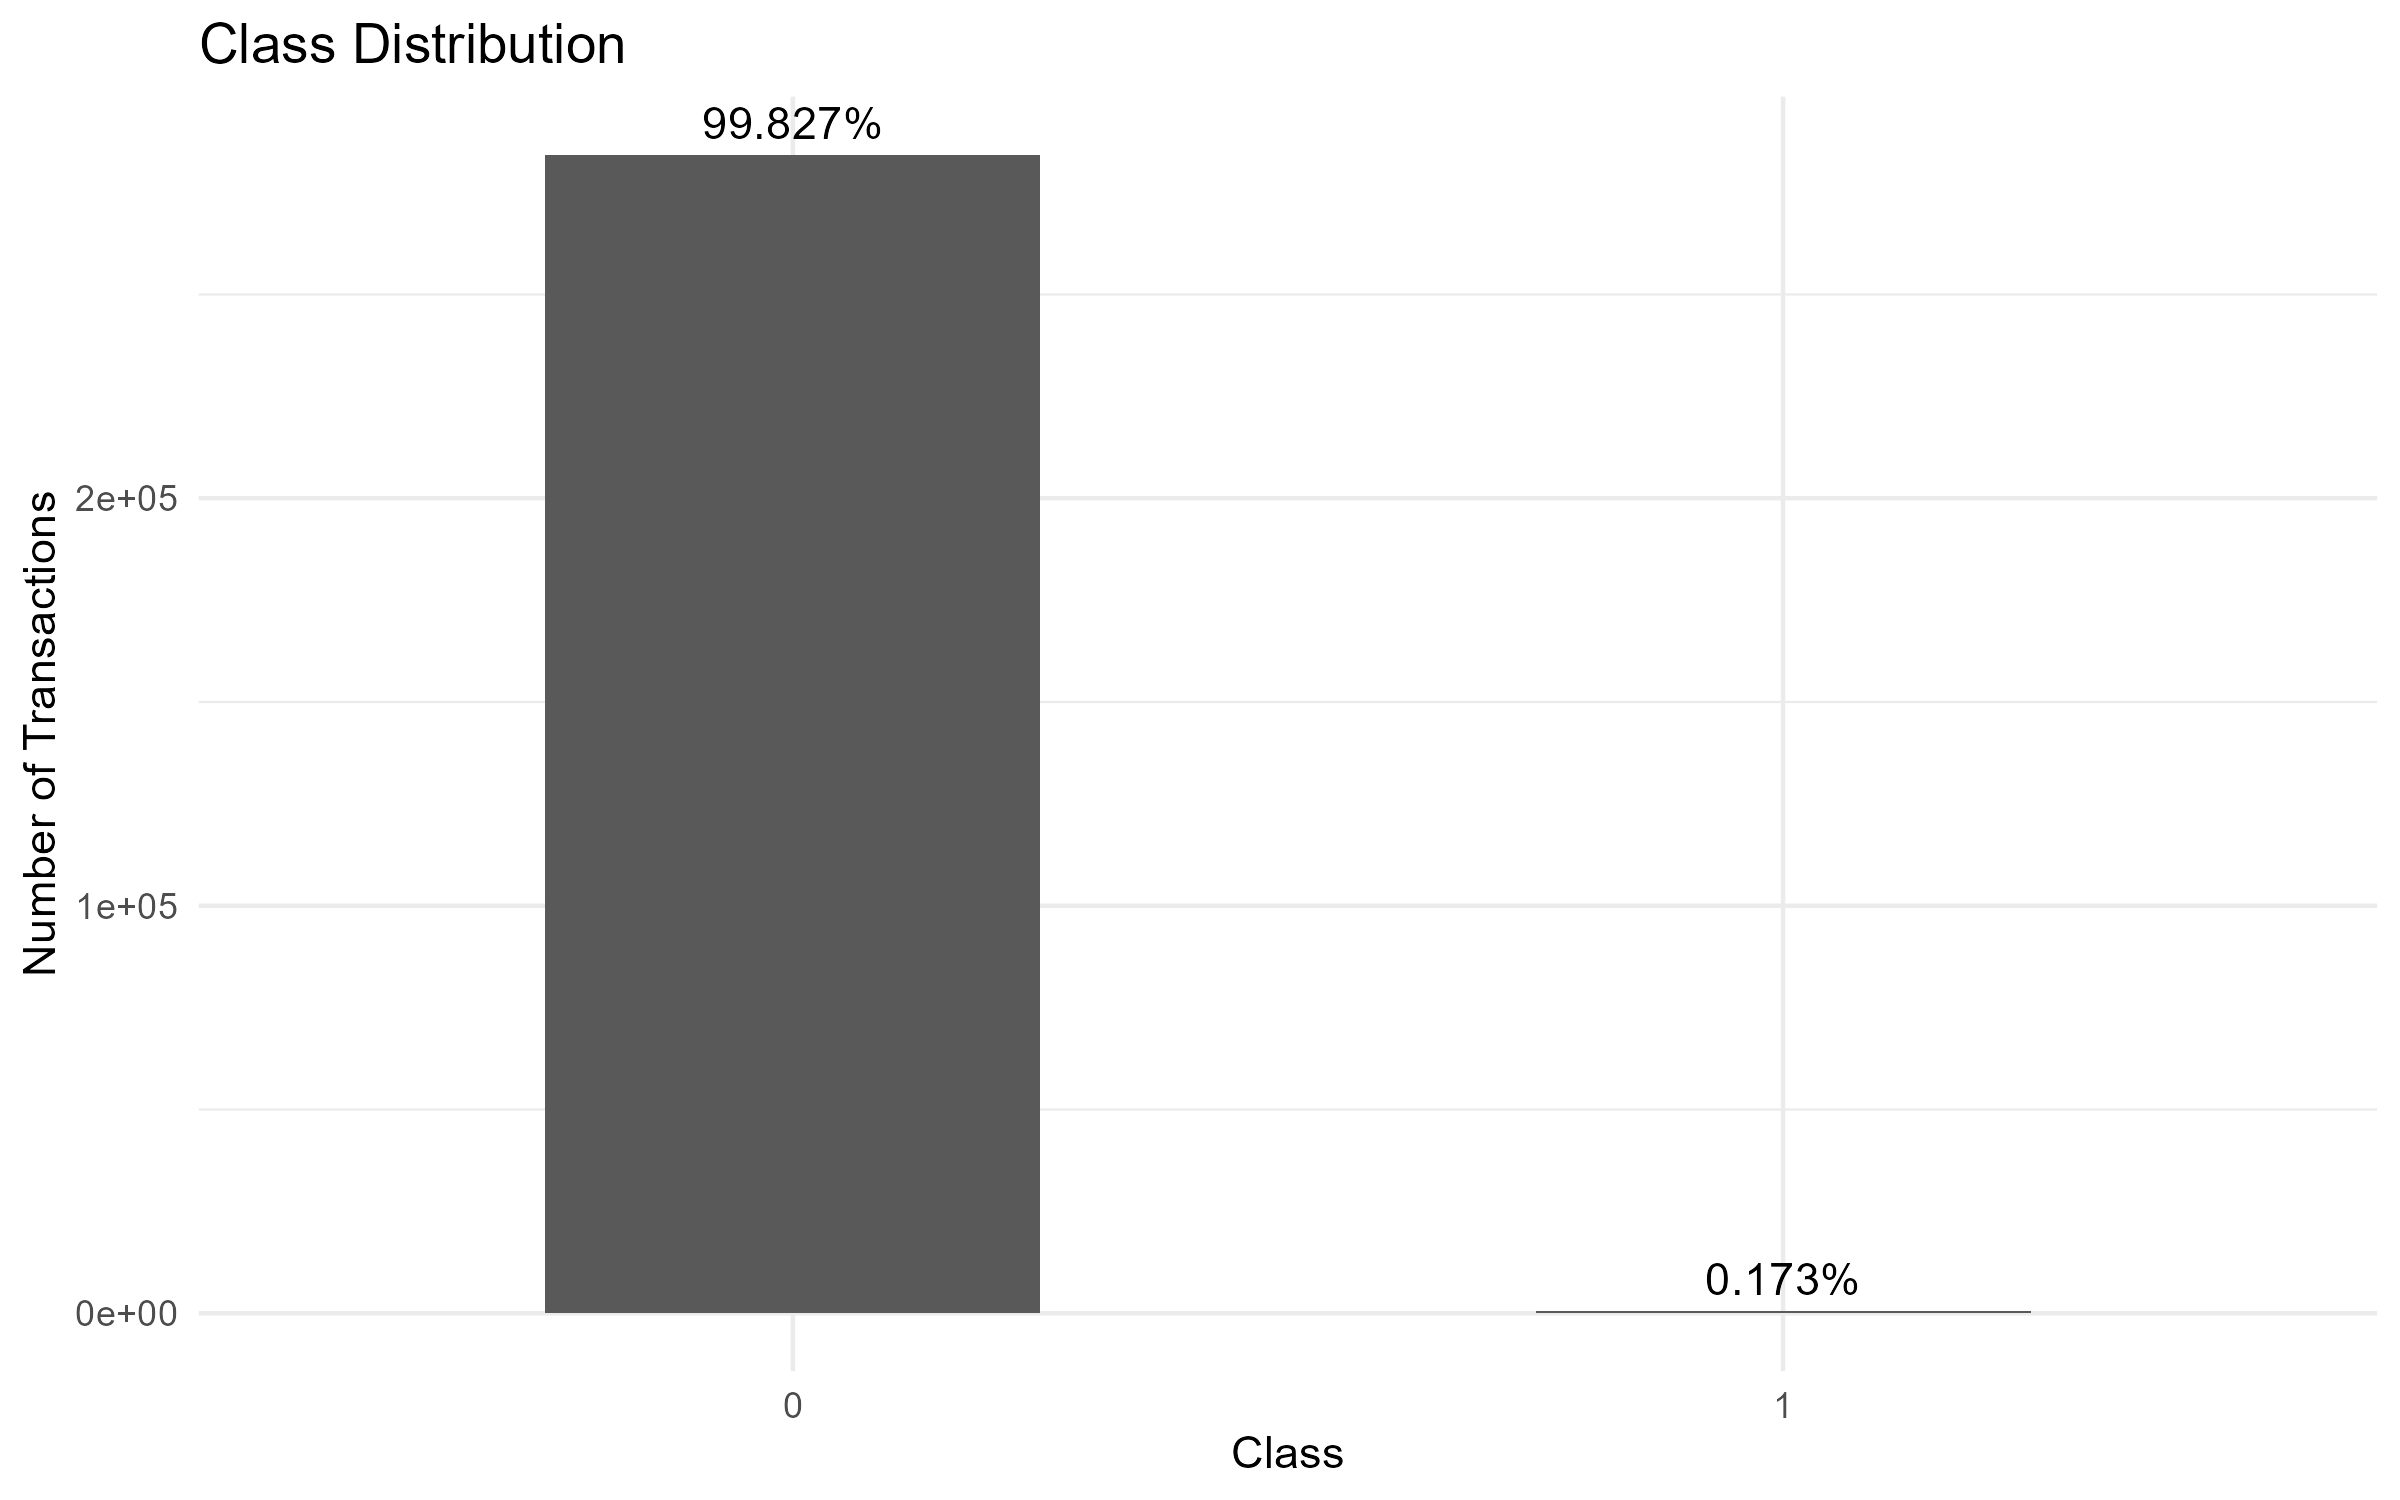
\includegraphics[keepaspectratio]{2-retail-analytics/../notebooks-and-scripts/2-retail-analytics/1-credit-card-fraud-detection-ml-benchmark/r/1-credit-card-fraud-detection-unsupervised-figures/class-distribution.png}}

}

\caption{\label{fig-class-distribution}Class distribution in the credit
card transaction dataset.}

\end{figure}%

Transaction amounts were also examined to characterize the range and
concentration of transaction values.

\begin{longtable}[]{@{}cc@{}}
\caption{Summary statistics for transaction
amounts.}\label{tbl-transaction-amount-summary}\tabularnewline
\toprule\noalign{}
Statistic & Value \\
\midrule\noalign{}
\endfirsthead
\toprule\noalign{}
Statistic & Value \\
\midrule\noalign{}
\endhead
\bottomrule\noalign{}
\endlastfoot
Minimum & 0.00 \\
1st Quartile & 5.60 \\
Median & 22.00 \\
Mean & 88.35 \\
3rd Quartile & 77.17 \\
Maximum & 25,691.16 \\
\end{longtable}

The distribution of transaction amounts is highly right-skewed, with
most transactions concentrated at relatively small values and a small
number of extreme observations. This behavior can be observed in
Figure~\ref{fig-transaction-amount-distribution}.

\begin{figure}

\centering{

\pandocbounded{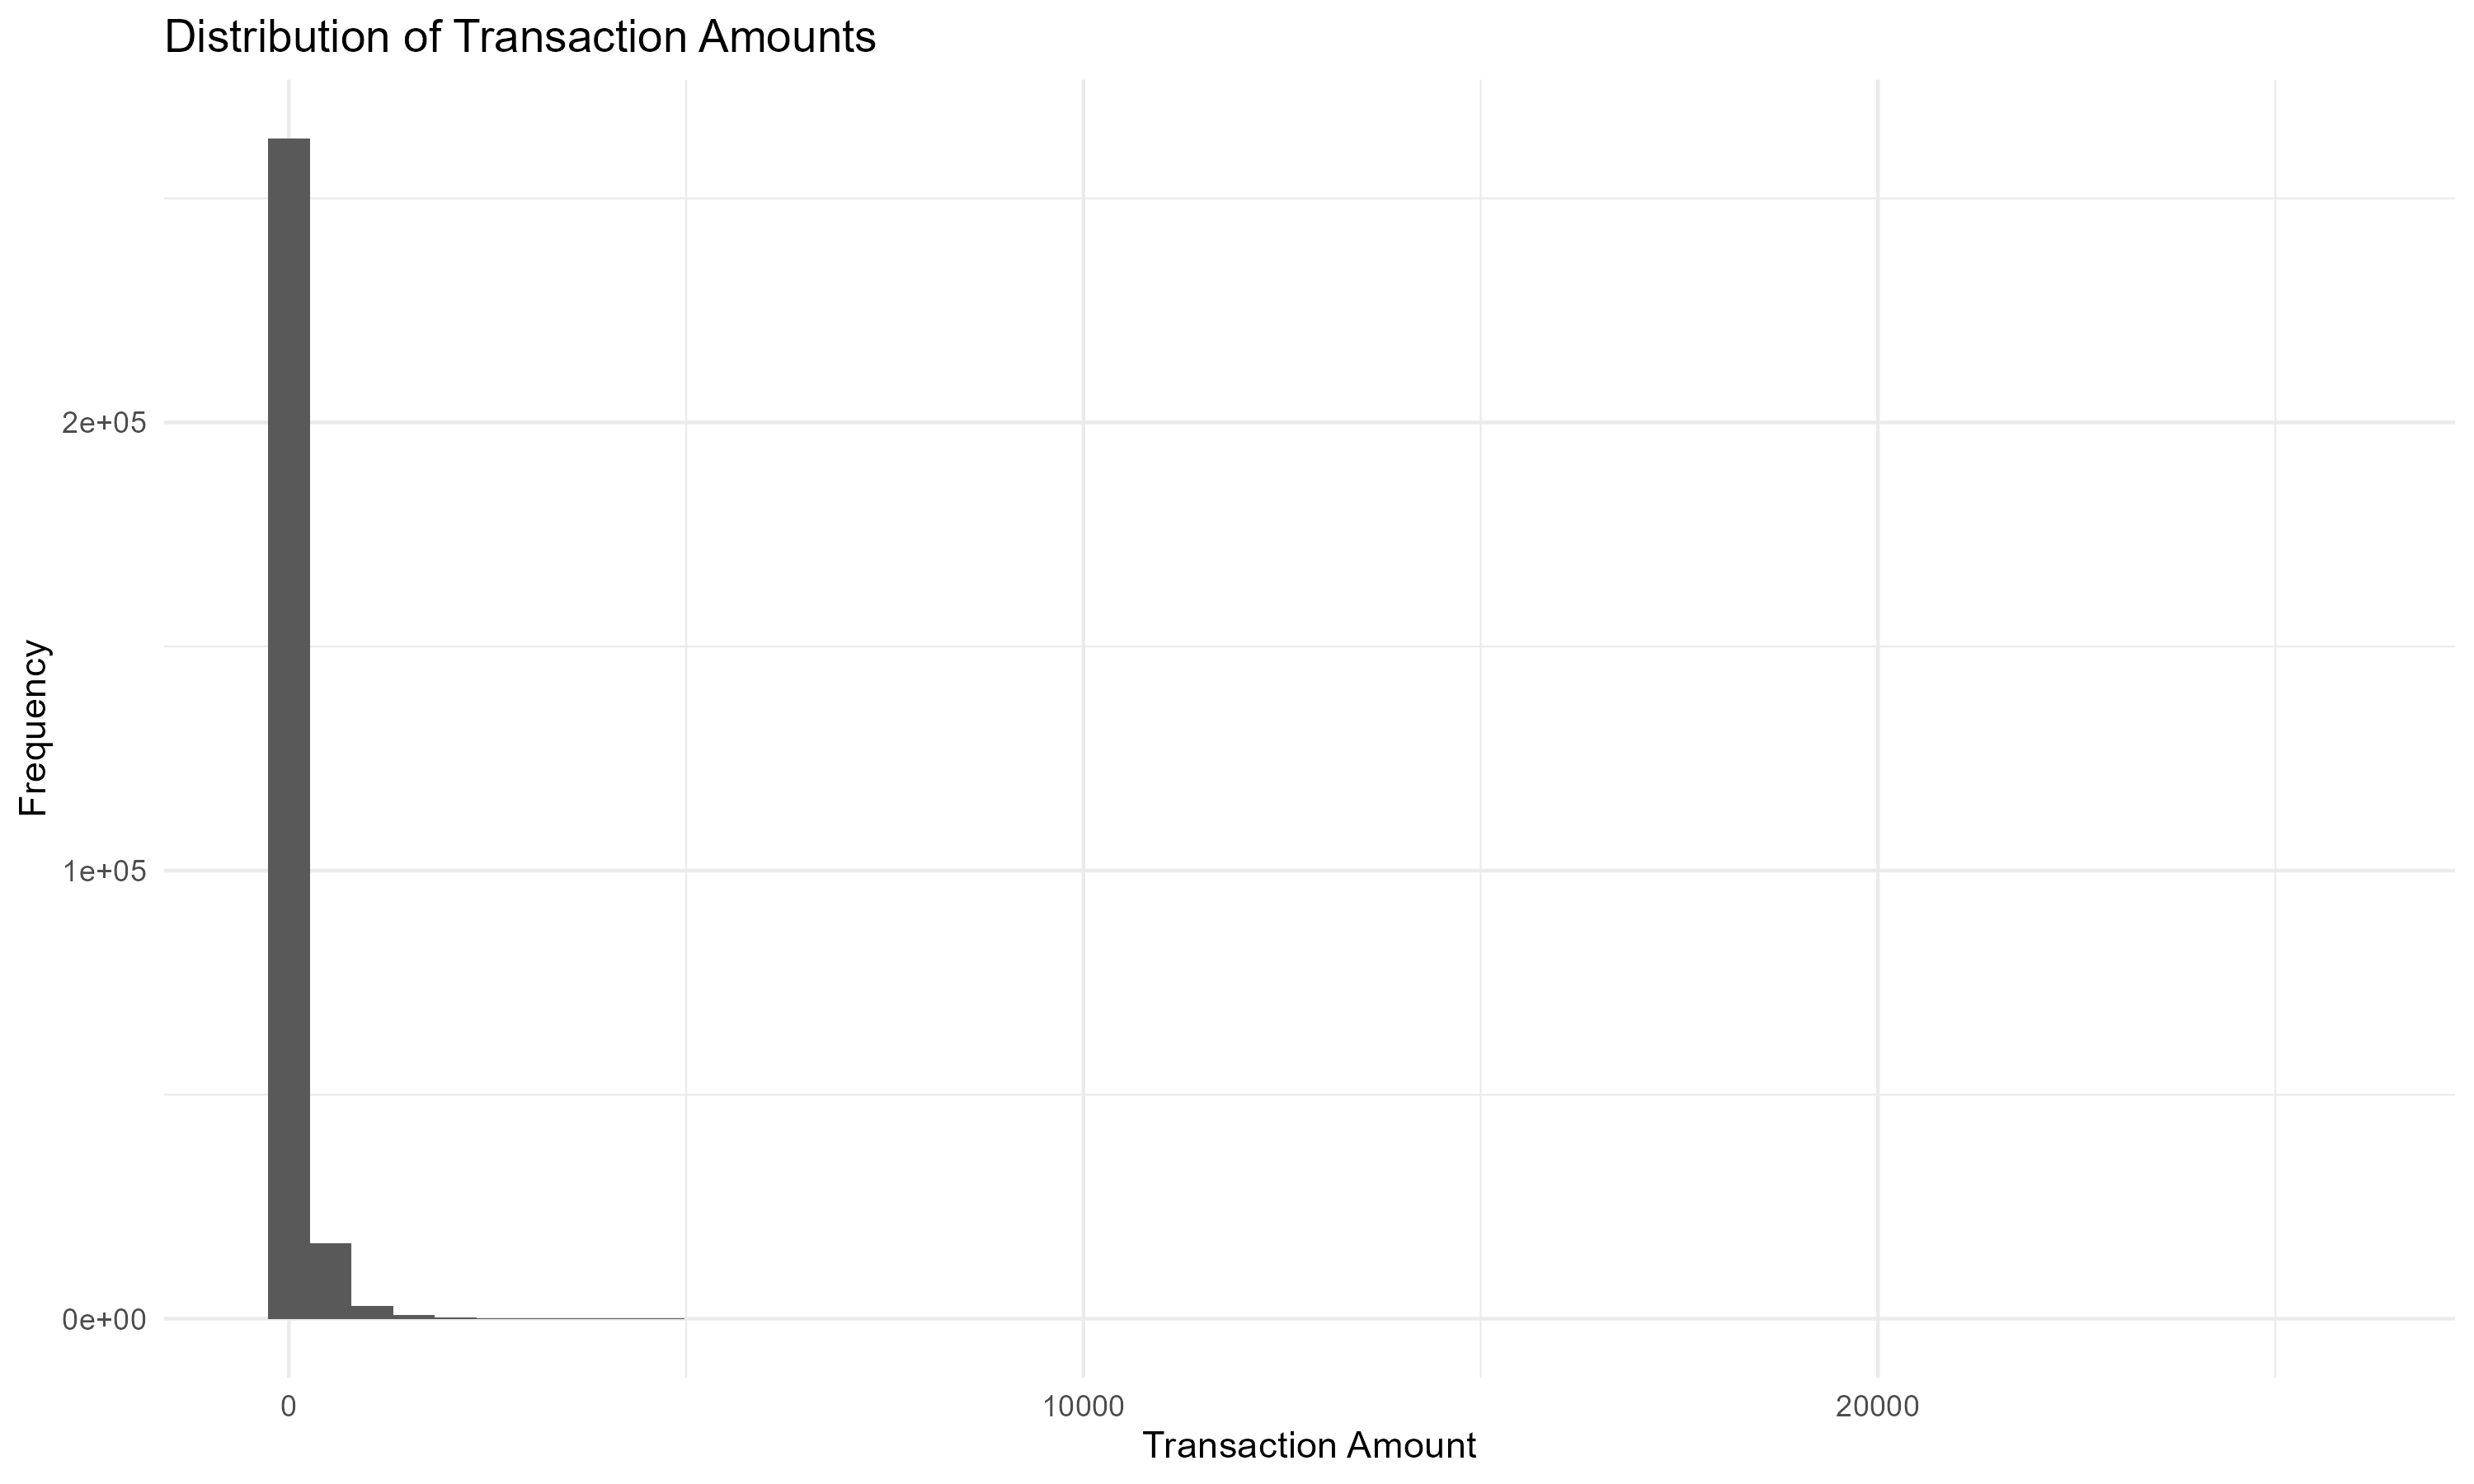
\includegraphics[keepaspectratio]{2-retail-analytics/../notebooks-and-scripts/2-retail-analytics/1-credit-card-fraud-detection-ml-benchmark/r/1-credit-card-fraud-detection-unsupervised-figures/transaction-amount-distribution.png}}

}

\caption{\label{fig-transaction-amount-distribution}Distribution of
transaction amounts.}

\end{figure}%

Transaction amounts were further compared across classes. Although
fraudulent and legitimate transactions overlap substantially,
Figure~\ref{fig-transaction-amount-by-class} suggests differences in the
distribution of transaction values between the two groups.

\begin{figure}

\centering{

\pandocbounded{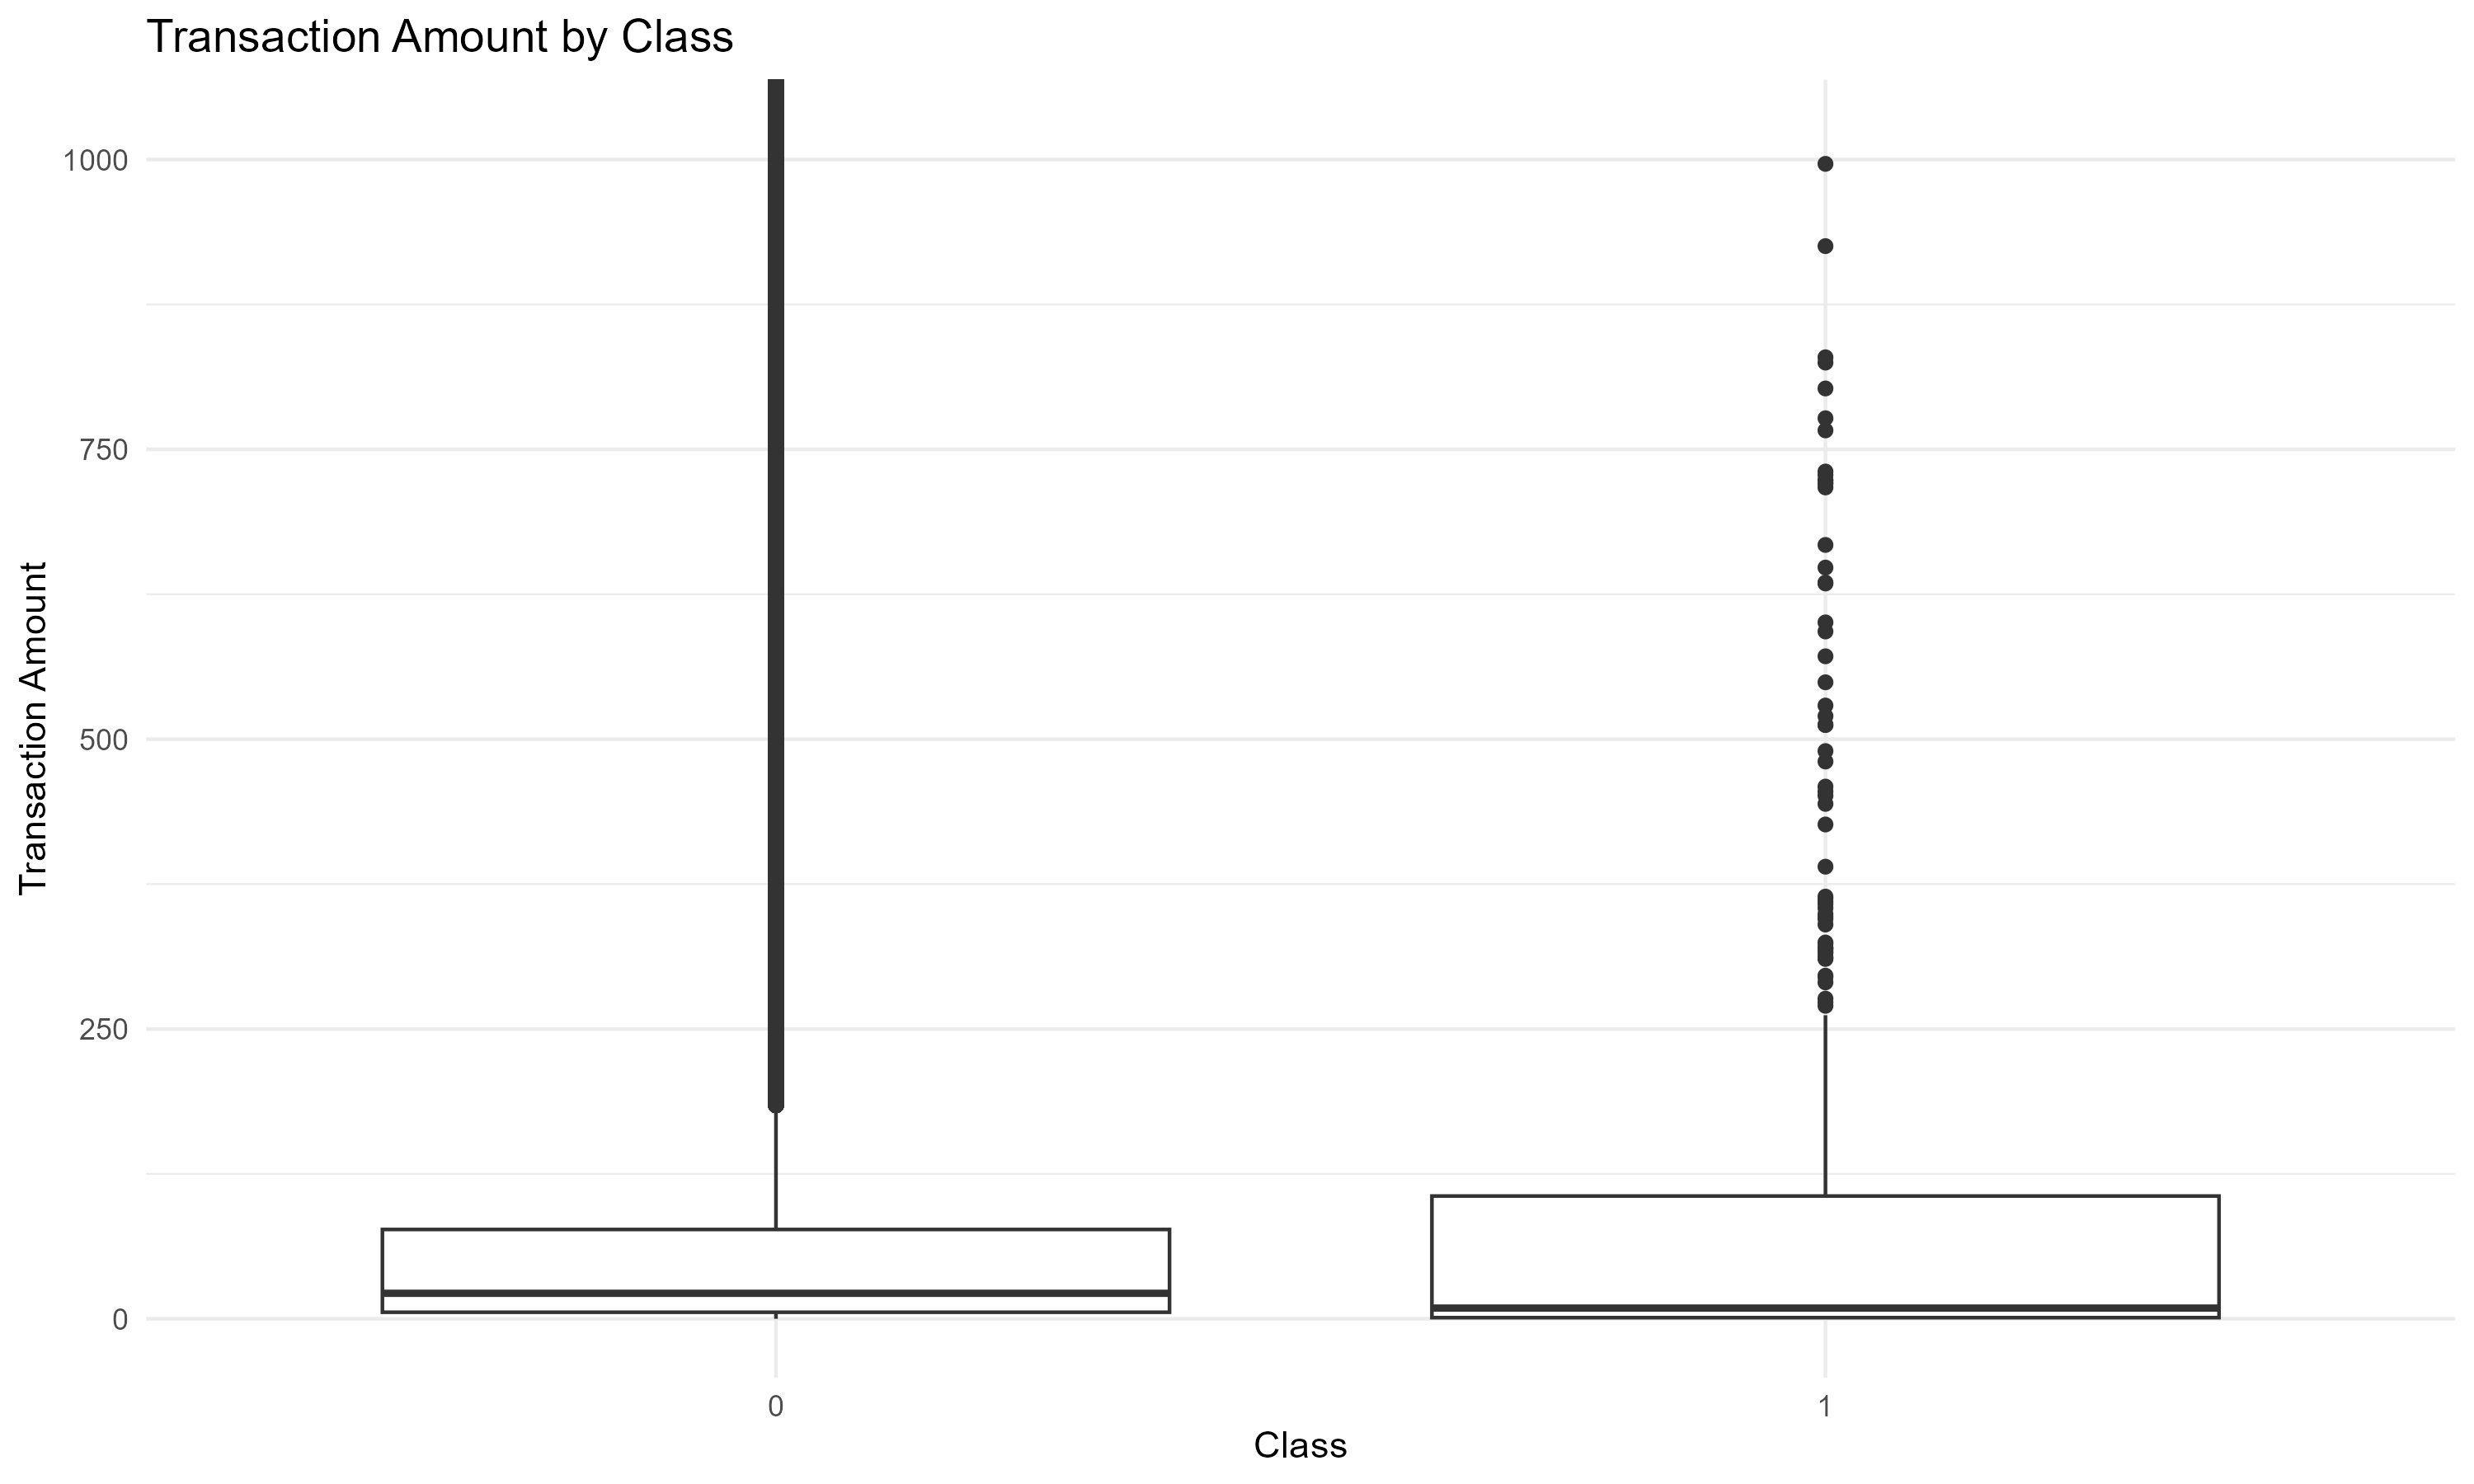
\includegraphics[keepaspectratio]{2-retail-analytics/../notebooks-and-scripts/2-retail-analytics/1-credit-card-fraud-detection-ml-benchmark/r/1-credit-card-fraud-detection-unsupervised-figures/transaction-amount-by-class.png}}

}

\caption{\label{fig-transaction-amount-by-class}Transaction amount by
class.}

\end{figure}%

The variables V1--V28 correspond to principal components obtained
through a prior anonymization process. Selected features were visualized
to examine differences between fraudulent and legitimate transactions.
Several variables exhibit noticeable shifts between classes, suggesting
that fraudulent transactions occupy distinct regions of the transformed
feature space.

\begin{figure}

\centering{

\pandocbounded{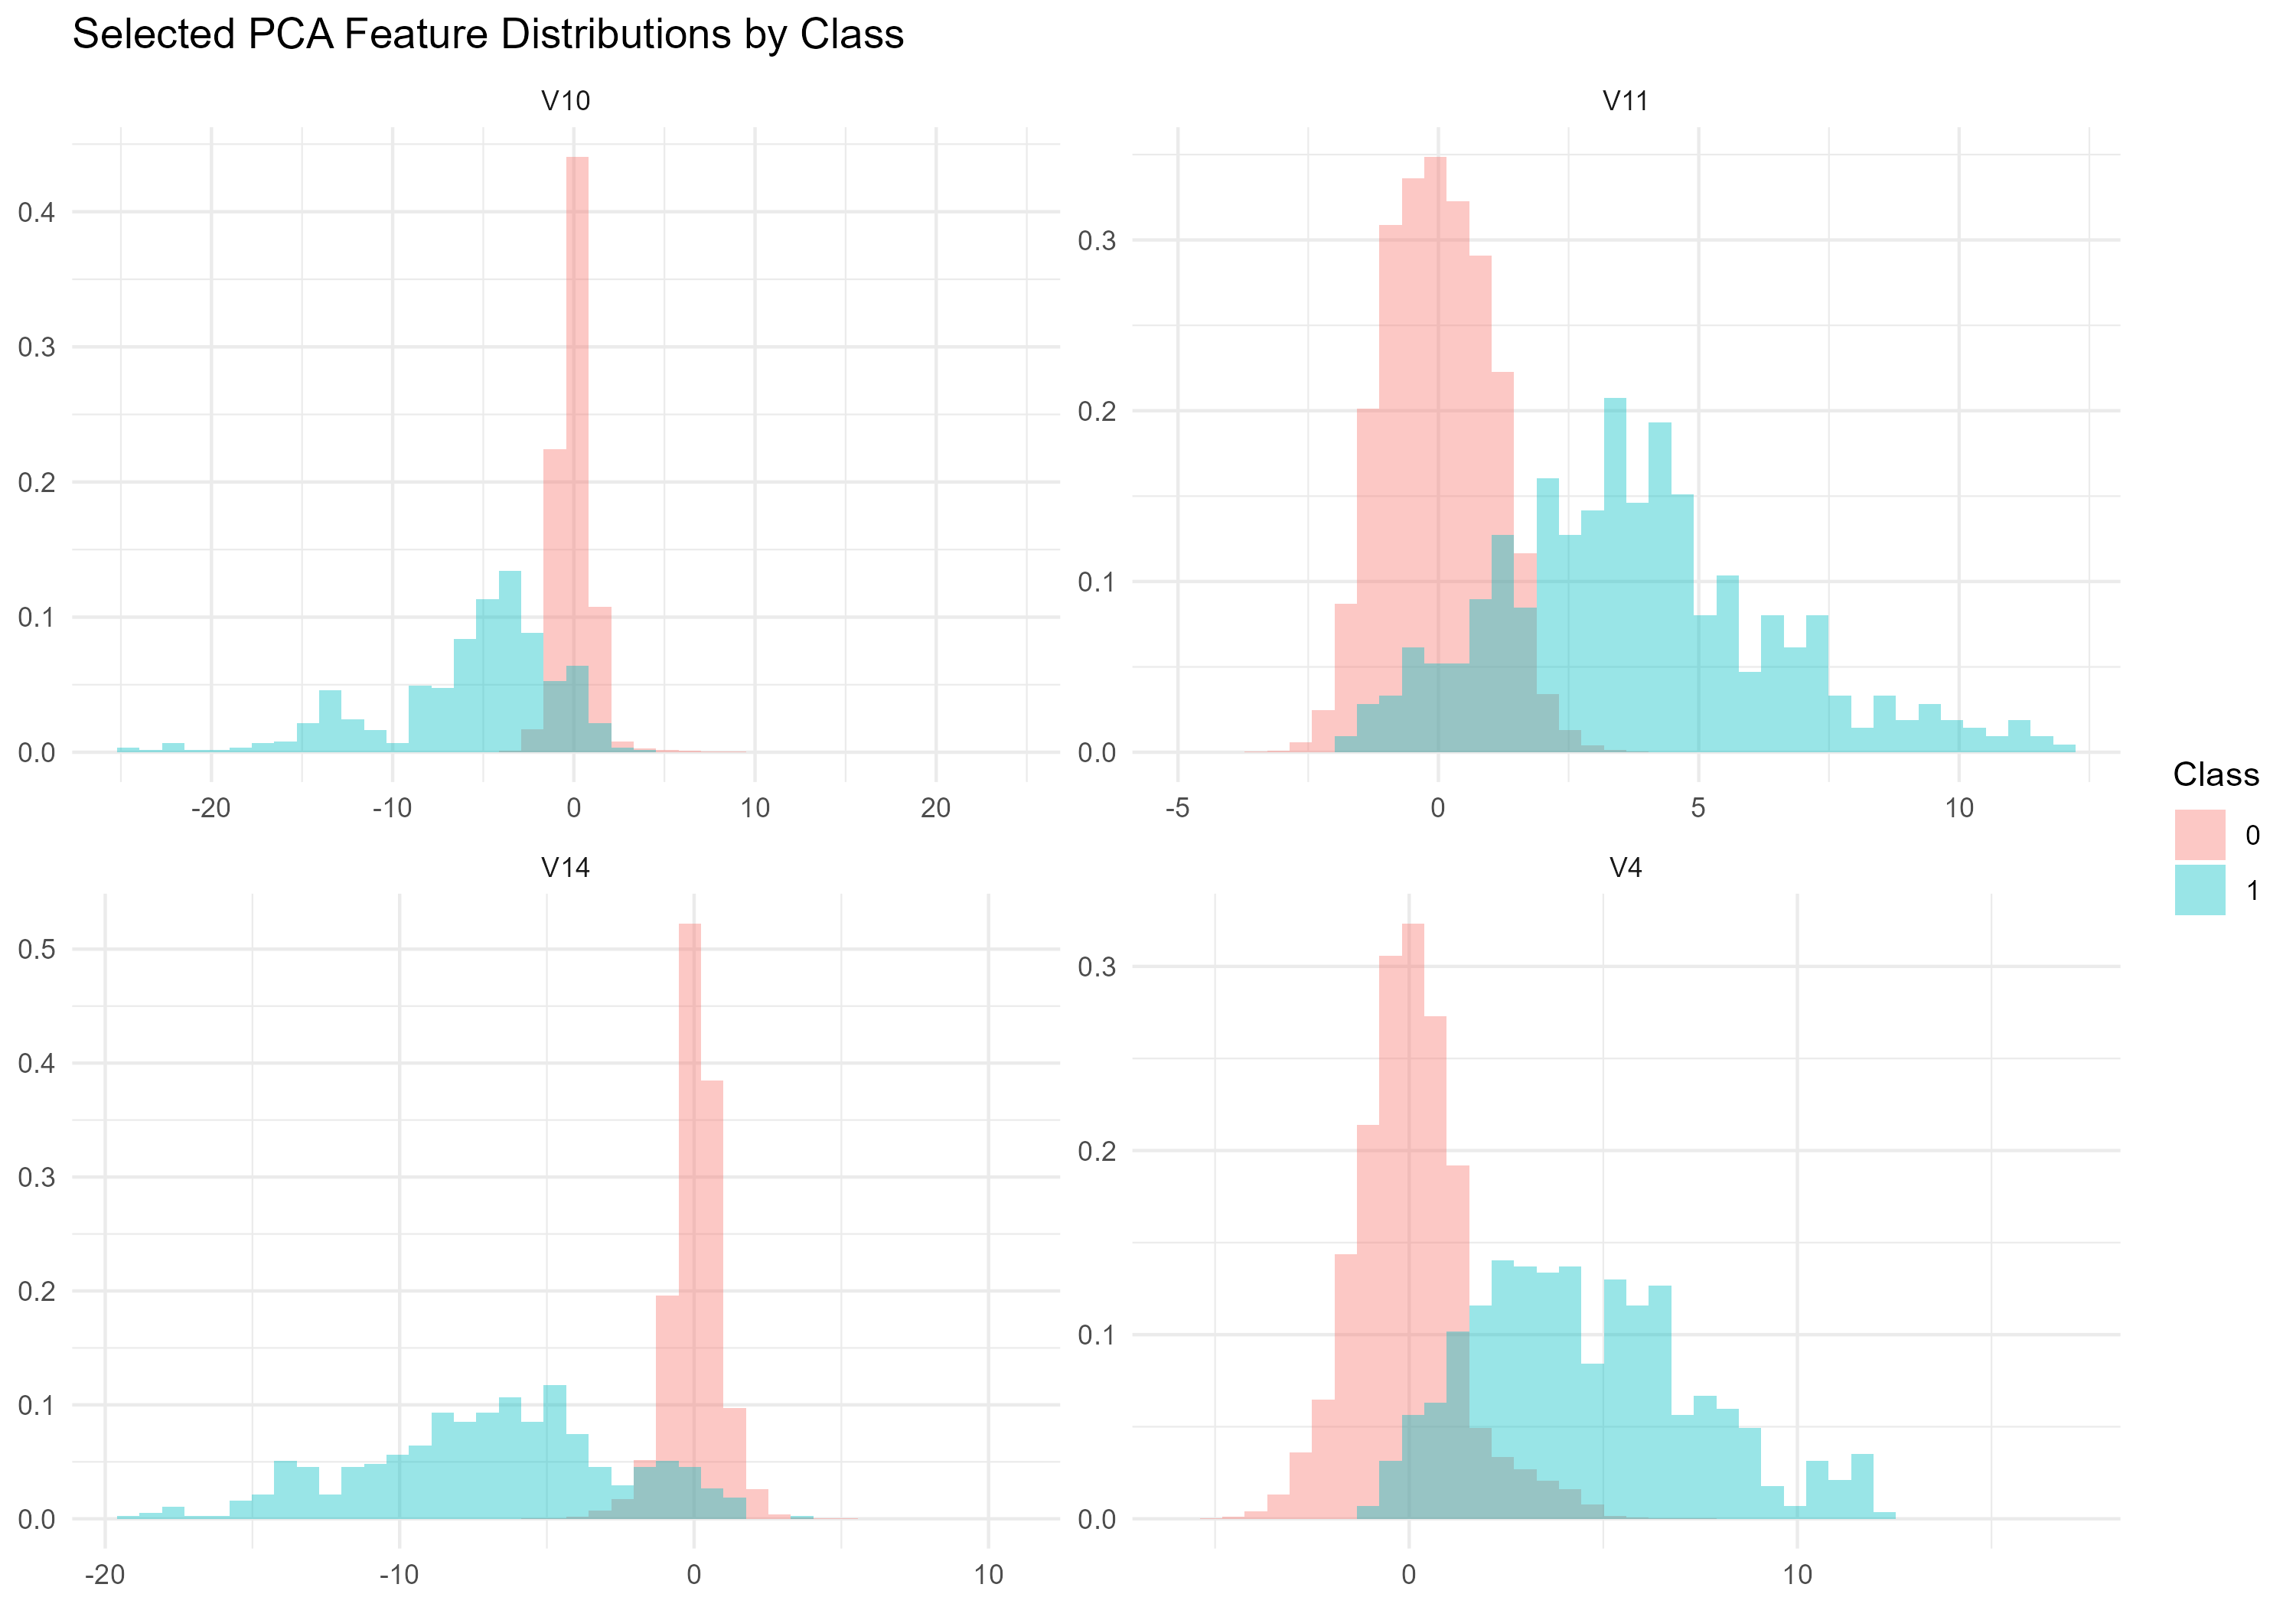
\includegraphics[keepaspectratio]{2-retail-analytics/../notebooks-and-scripts/2-retail-analytics/1-credit-card-fraud-detection-ml-benchmark/r/1-credit-card-fraud-detection-unsupervised-figures/selected-pca-features-distribution.png}}

}

\caption{\label{fig-selected-pca-features}Selected PCA feature
distributions by class.}

\end{figure}%

To complement the univariate analysis, a correlation matrix was computed
using all available variables.

\begin{figure}

\centering{

\pandocbounded{
\includegraphics[keepaspectratio]{2-retail-analytics/../notebooks-and-scripts/2-retail-analytics/1-credit-card-fraud-detection-ml-benchmark/r/1-credit-card-fraud-detection-unsupervised-figures/correlation-matrix.png}}

}

\caption{\label{fig-correlation-matrix}Correlation matrix of the credit
card transaction dataset.}

\end{figure}%

Following the exploratory analysis, the target variable was separated
from the predictors and the Time variable was removed. The data was then
partitioned into training and test sets using stratified sampling to
preserve the original class distribution. Feature scaling was applied
after the train-test split, with scaling parameters estimated
exclusively from the training data.

Because the training set contains more than two hundred thousand
observations, a stratified sample was extracted from the training data
for the clustering analysis. The sample preserves the original fraud
rate while reducing computational requirements and allowing a consistent
comparison across clustering algorithms.

Three clustering approaches were evaluated:

\begin{itemize}
\tightlist
\item
  K-Means Clustering
\item
  Agglomerative Clustering
\item
  DBSCAN
\end{itemize}

For K-Means, multiple values of (k) were explored. The elbow method was
evaluated using the within-cluster sum of squares (inertia).

\begin{figure}

\centering{

\pandocbounded{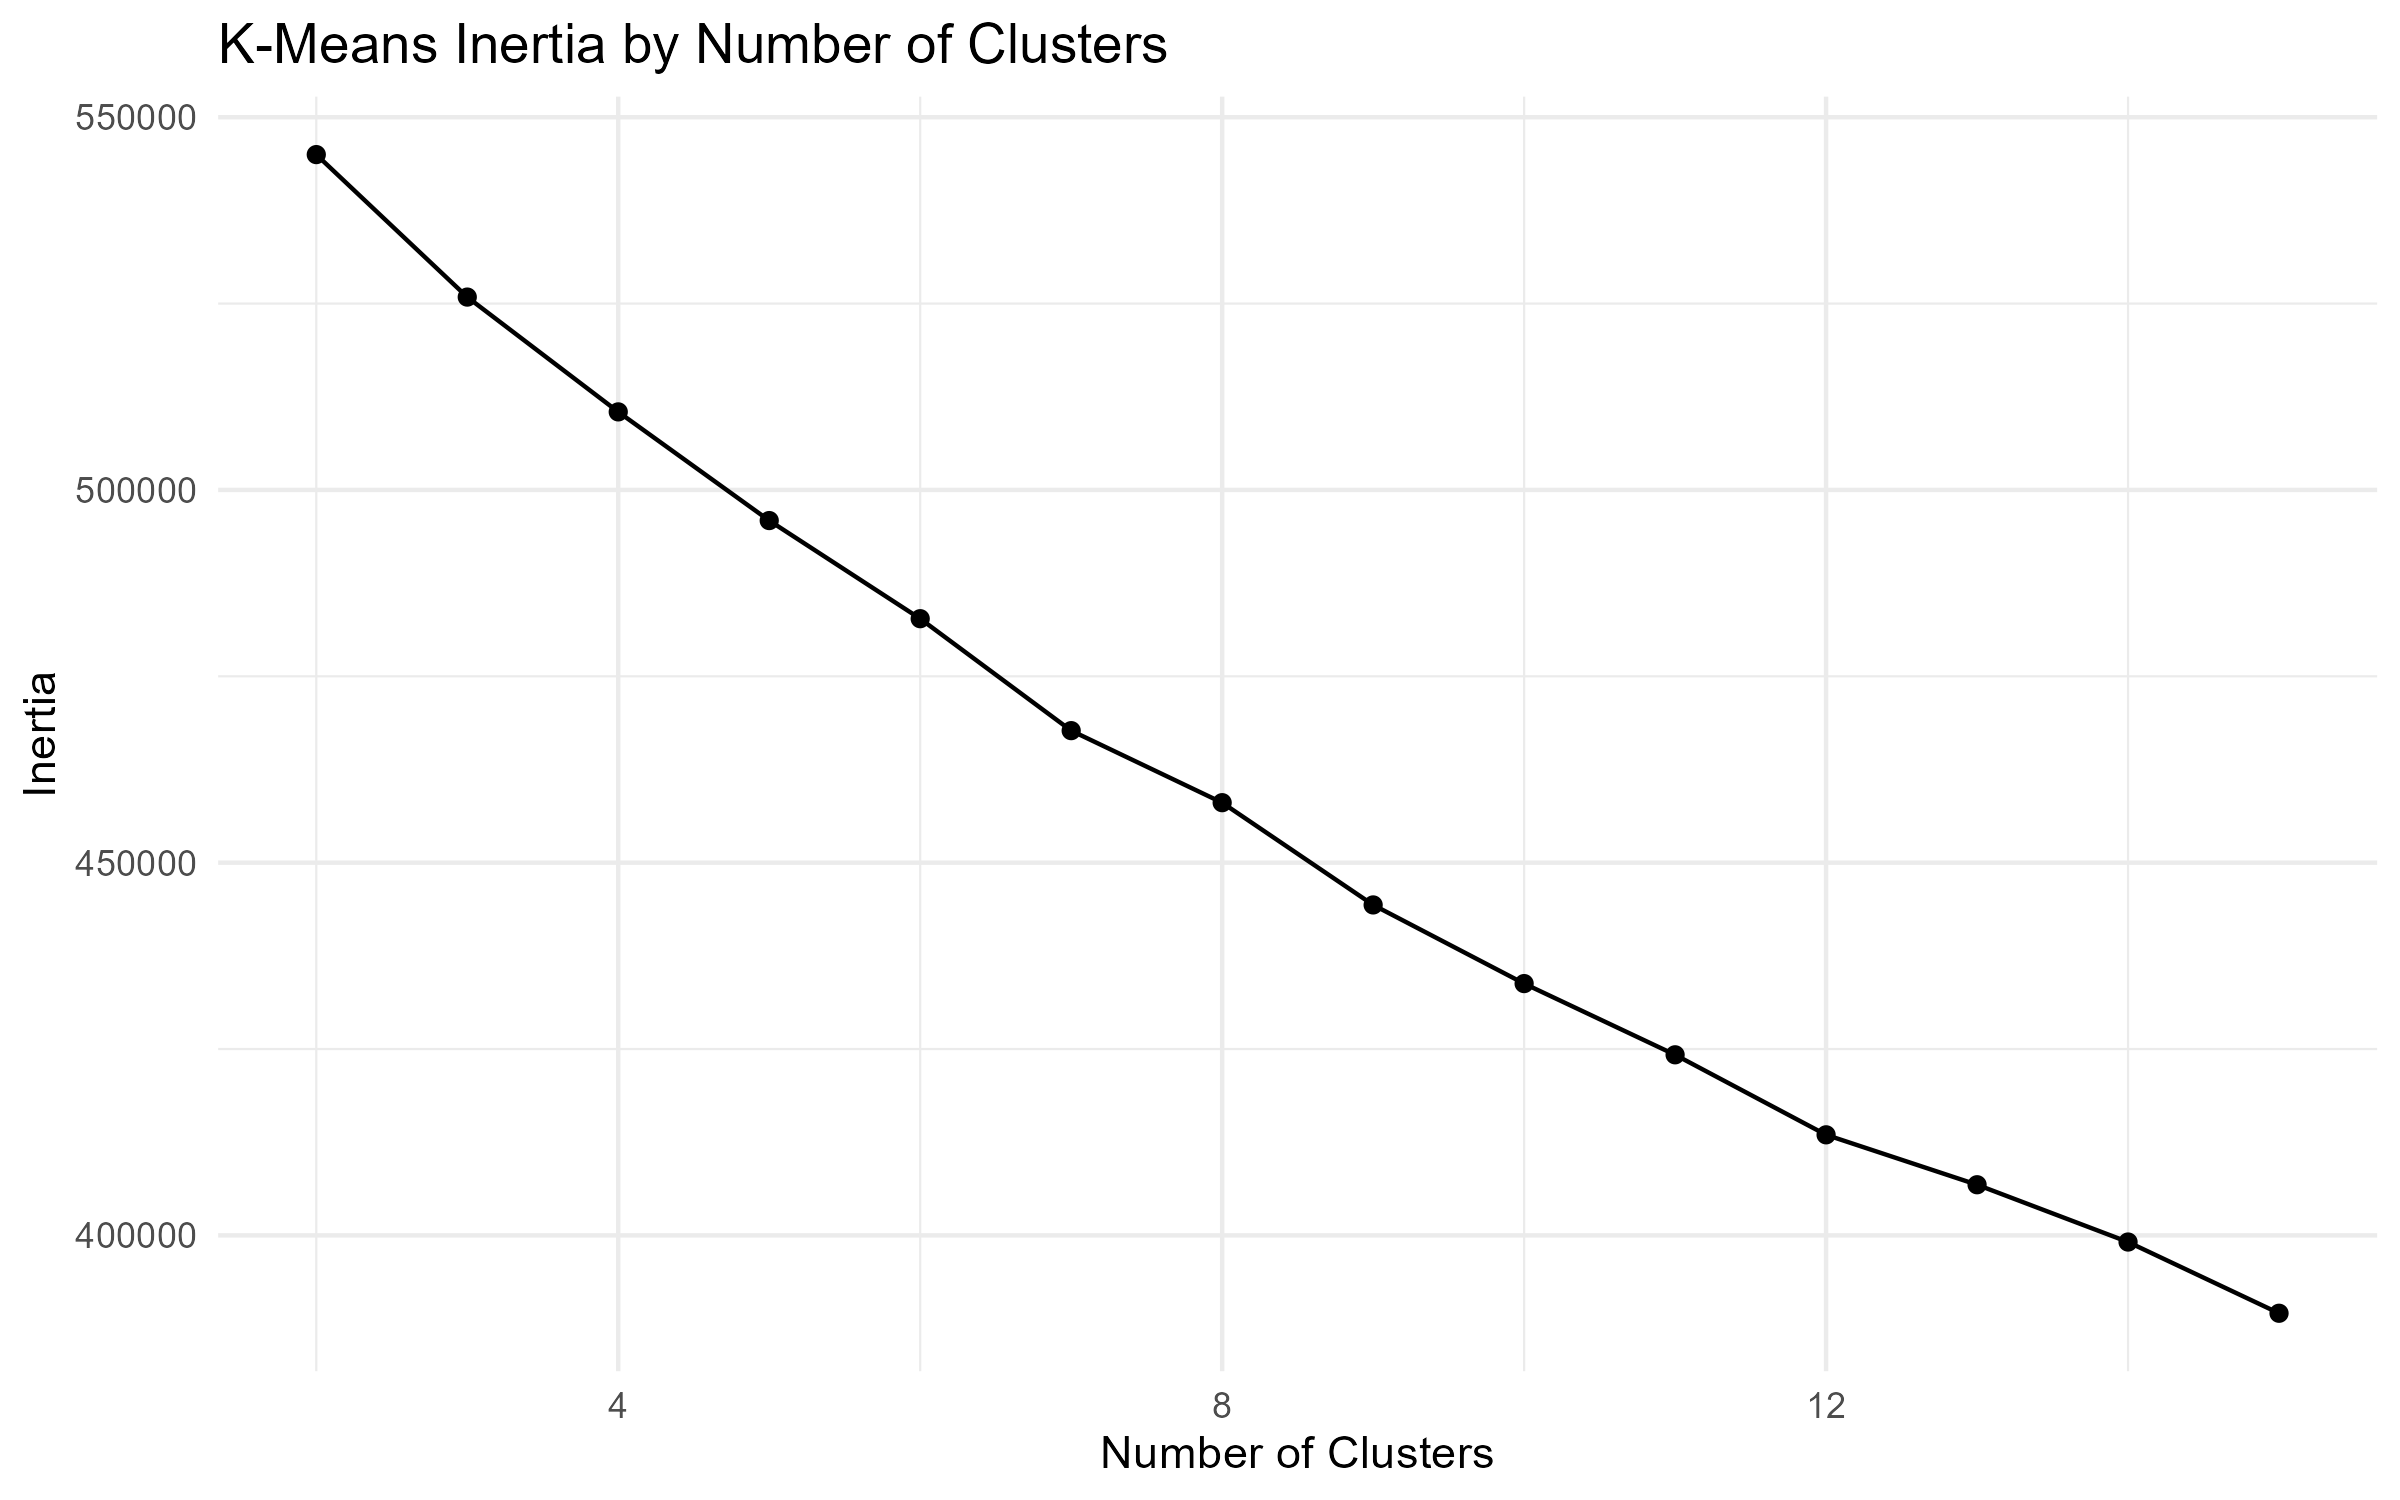
\includegraphics[keepaspectratio]{2-retail-analytics/../notebooks-and-scripts/2-retail-analytics/1-credit-card-fraud-detection-ml-benchmark/r/1-credit-card-fraud-detection-unsupervised-figures/kmeans-inertia.png}}

}

\caption{\label{fig-kmeans-inertia}K-Means inertia as a function of the
number of clusters.}

\end{figure}%

The elbow plot does not reveal a clear point at which additional
clusters provide diminishing returns. As a result, the number of
clusters cannot be determined reliably using inertia alone. Additional
validation metrics were evaluated and used as complementary diagnostic
tools. Since no single criterion produced a definitive solution, the
final choice was guided by interpretability and fraud concentration
within the resulting clusters.

A three-cluster solution was retained because it revealed the strongest
concentration of fraudulent transactions while remaining straightforward
to interpret.

The composition of the resulting clusters was then examined by comparing
cluster-level fraud rates against the baseline fraud rate observed in
the clustering sample.

\begin{longtable}[]{@{}
  >{\centering\arraybackslash}p{(\linewidth - 2\tabcolsep) * \real{0.1970}}
  >{\centering\arraybackslash}p{(\linewidth - 2\tabcolsep) * \real{0.8030}}@{}}
\caption{Summary of the main findings obtained from the clustering
algorithms.}\label{tbl-clustering-summary}\tabularnewline
\toprule\noalign{}
\begin{minipage}[b]{\linewidth}\centering
Method
\end{minipage} & \begin{minipage}[b]{\linewidth}\centering
Key Finding
\end{minipage} \\
\midrule\noalign{}
\endfirsthead
\toprule\noalign{}
\begin{minipage}[b]{\linewidth}\centering
Method
\end{minipage} & \begin{minipage}[b]{\linewidth}\centering
Key Finding
\end{minipage} \\
\midrule\noalign{}
\endhead
\bottomrule\noalign{}
\endlastfoot
K-Means & One cluster exhibited a fraud rate approximately 21 times
higher than the baseline fraud rate. \\
Agglomerative Clustering & A small cluster exhibited a fraud rate
approximately 490 times higher than the baseline fraud rate. \\
DBSCAN & Fraudulent transactions were primarily identified as noise
points rather than members of dense clusters. \\
\end{longtable}

The clustering results provide complementary perspectives on the
structure of fraudulent transactions. K-Means identified a relatively
large region characterized by elevated fraud concentration, while
Agglomerative Clustering isolated a much smaller cluster with an
exceptionally high fraud rate. In contrast, DBSCAN classified fraudulent
transactions primarily as noise, suggesting that some fraud patterns
behave as isolated anomalies rather than members of dense groups.

Taken together, these results indicate that fraudulent transactions are
not uniformly distributed across the feature space. Although the exact
structure varies across clustering algorithms, all three methods reveal
behavior that differs substantially from the baseline distribution of
legitimate transactions.

These findings provide preliminary evidence that fraudulent transactions
leave detectable signatures in the available feature space and motivate
the supervised learning stage of the analysis.

Additional implementation details, including the companion Quarto and
Python notebooks, are available in the project repository
\href{https://github.com/rodrigokang/portfolio/tree/main/notebooks-and-scripts/2-retail-analytics/1-credit-card-fraud-detection-ml-benchmark}{\faGithub}

\subsection{Supervised Learning
Benchmark}\label{supervised-learning-benchmark}

The supervised stage uses the transaction labels to evaluate how well
different classification models can identify fraudulent transactions.
The purpose is not to find a model that looks good under a single
metric, but to compare modelling choices under conditions that resemble
the operational reality of fraud detection: the positive class is rare,
the cost of missed fraud is not the same as the cost of a false alarm,
and a model that performs well on average may still be unhelpful if it
fails to rank suspicious transactions near the top.

The benchmark was implemented in two complementary forms. The Python
notebook runs the full comparison across the complete set of candidate
algorithms and class imbalance strategies. The R / Quarto notebook
focuses on the two retained configurations that are most useful for the
final discussion: a Random Forest trained on the original class
distribution, and an XGBoost model trained after applying SMOTE. This
split keeps the implementation practical while preserving the main
modelling comparison.

The training and test sets were created using stratified sampling so
that the rare fraud class remained represented in both subsets. Scaling
was estimated from the training data only and then applied to the test
data, avoiding leakage from unseen transactions into the model
preparation step. This is especially important in fraud detection, where
small forms of leakage can make a model appear much stronger than it
would be in deployment.

The original training distribution is shown in
Table~\ref{tbl-class-distribution-training-strategies}. The table also
shows the SMOTE-resampled version used by the XGBoost model. The
resampled dataset is balanced for training purposes only; the test set
remains in the original imbalanced distribution.

\begin{longtable}[]{@{}lccc@{}}
\caption{Class distribution by training
strategy.}\label{tbl-class-distribution-training-strategies}\tabularnewline
\toprule\noalign{}
Strategy & Class & Transactions & Percentage (\%) \\
\midrule\noalign{}
\endfirsthead
\toprule\noalign{}
Strategy & Class & Transactions & Percentage (\%) \\
\midrule\noalign{}
\endhead
\bottomrule\noalign{}
\endlastfoot
Original & Legitimate & 227,446 & 99.825 \\
Original & Fraudulent & 399 & 0.175 \\
SMOTE & Legitimate & 227,446 & 50.000 \\
SMOTE & Fraudulent & 227,446 & 50.000 \\
\end{longtable}

Three imbalance strategies were considered in the broader supervised
benchmark: the original class distribution, random undersampling, and
SMOTE. The original distribution preserves the natural frequency of
fraud, which is useful because it reflects the problem as it is
encountered in practice. Random undersampling creates a balanced
training set by removing legitimate transactions, which may help some
models learn the minority class but also discards a large amount of
information. SMOTE creates synthetic minority-class observations,
allowing the model to see a denser representation of the fraud region
without removing legitimate transactions.

The evaluation framework uses precision, recall, F1-score, ROC-AUC,
Precision-Recall AUC, and the Kolmogorov-Smirnov statistic. In this
setting, accuracy is deliberately avoided as a headline metric. With
fraud representing only \(0.173\%\) of transactions, a classifier could
obtain high accuracy by predicting almost everything as legitimate.

Precision measures how many flagged transactions are actually
fraudulent:

\begin{equation}\phantomsection\label{eq-precision}{
\text{Precision} = \frac{TP}{TP + FP}
}\end{equation}

Recall measures how many fraudulent transactions are successfully
identified:

\begin{equation}\phantomsection\label{eq-recall}{
\text{Recall} = \frac{TP}{TP + FN}
}\end{equation}

The F1-score combines both quantities into a single summary:

\begin{equation}\phantomsection\label{eq-f1-score}{
F_1 = 2 \cdot \frac{\text{Precision} \cdot \text{Recall}}{\text{Precision} + \text{Recall}}
}\end{equation}

For model selection, Precision-Recall AUC is particularly important
because it focuses on the minority class. ROC-AUC remains useful, but
under severe imbalance it can sometimes look reassuring even when the
model generates too many false positives for practical use. The KS
statistic adds a further diagnostic view by measuring the maximum
separation between the empirical score distributions of legitimate and
fraudulent transactions.

The broader Python benchmark selected one leading model from each
imbalance strategy. Random Forest performed best under the original
class distribution, while XGBoost was the strongest model under both
undersampling and SMOTE. The final test-set inspection then focused on
whether those benchmark findings translated to unseen transactions.

In the final R / Quarto implementation, the comparison was narrowed to
the two most informative retained configurations. Random Forest trained
on the original class distribution represents the best-performing model
that does not alter the training distribution. XGBoost with SMOTE
represents the strongest imbalance-aware alternative. The
undersampling-based XGBoost model was not retained for the final
comparison because, despite strong cross-validation results on the
balanced training data, its test-set behaviour produced too many false
positives to be attractive as a practical fraud-screening model.

The final comparison is summarized in
Table~\ref{tbl-final-model-comparison}.

\begin{longtable}[]{@{}
  >{\centering\arraybackslash}p{(\linewidth - 14\tabcolsep) * \real{0.1183}}
  >{\centering\arraybackslash}p{(\linewidth - 14\tabcolsep) * \real{0.1720}}
  >{\centering\arraybackslash}p{(\linewidth - 14\tabcolsep) * \real{0.1290}}
  >{\centering\arraybackslash}p{(\linewidth - 14\tabcolsep) * \real{0.0968}}
  >{\centering\arraybackslash}p{(\linewidth - 14\tabcolsep) * \real{0.1183}}
  >{\centering\arraybackslash}p{(\linewidth - 14\tabcolsep) * \real{0.1075}}
  >{\centering\arraybackslash}p{(\linewidth - 14\tabcolsep) * \real{0.0968}}
  >{\centering\arraybackslash}p{(\linewidth - 14\tabcolsep) * \real{0.1613}}@{}}
\caption{Final model comparison on the test
set.}\label{tbl-final-model-comparison}\tabularnewline
\toprule\noalign{}
\begin{minipage}[b]{\linewidth}\centering
Strategy
\end{minipage} & \begin{minipage}[b]{\linewidth}\centering
Model
\end{minipage} & \begin{minipage}[b]{\linewidth}\centering
Precision
\end{minipage} & \begin{minipage}[b]{\linewidth}\centering
Recall
\end{minipage} & \begin{minipage}[b]{\linewidth}\centering
F1-score
\end{minipage} & \begin{minipage}[b]{\linewidth}\centering
ROC-AUC
\end{minipage} & \begin{minipage}[b]{\linewidth}\centering
PR-AUC
\end{minipage} & \begin{minipage}[b]{\linewidth}\centering
KS statistic
\end{minipage} \\
\midrule\noalign{}
\endfirsthead
\toprule\noalign{}
\begin{minipage}[b]{\linewidth}\centering
Strategy
\end{minipage} & \begin{minipage}[b]{\linewidth}\centering
Model
\end{minipage} & \begin{minipage}[b]{\linewidth}\centering
Precision
\end{minipage} & \begin{minipage}[b]{\linewidth}\centering
Recall
\end{minipage} & \begin{minipage}[b]{\linewidth}\centering
F1-score
\end{minipage} & \begin{minipage}[b]{\linewidth}\centering
ROC-AUC
\end{minipage} & \begin{minipage}[b]{\linewidth}\centering
PR-AUC
\end{minipage} & \begin{minipage}[b]{\linewidth}\centering
KS statistic
\end{minipage} \\
\midrule\noalign{}
\endhead
\bottomrule\noalign{}
\endlastfoot
Original & Random Forest & 0.9625 & 0.8280 & 0.8902 & 0.9656 & 0.8782 &
0.9056 \\
SMOTE & XGBoost & 0.7080 & 0.8602 & 0.7767 & 0.9823 & 0.8594 & 0.9040 \\
\end{longtable}

The two models make a useful trade-off visible. Random Forest is more
conservative. It achieves higher precision, a higher F1-score, and the
strongest Precision-Recall AUC. In practical terms, when it flags a
transaction as fraudulent, it is more likely to be correct. This matters
because false alarms are not free: they can block legitimate purchases,
inconvenience customers, and create manual review work.

XGBoost with SMOTE is more aggressive. It achieves higher recall and a
higher ROC-AUC, meaning it captures a larger share of the fraudulent
transactions and ranks the two classes well across thresholds. The cost
is lower precision: more legitimate transactions are pulled into the
fraud queue. Depending on the operational context, this may still be
acceptable. A bank or payment provider with a low-friction review
process may prefer higher recall, while a retailer or platform with a
strong customer-experience focus may place greater weight on precision.

Figure~\ref{fig-final-model-comparison-pr-auc} compares the retained
models using Precision-Recall AUC. The difference is not large, but
Random Forest remains slightly ahead on the metric that is most directly
aligned with rare-event detection.

\begin{figure}

\centering{

\pandocbounded{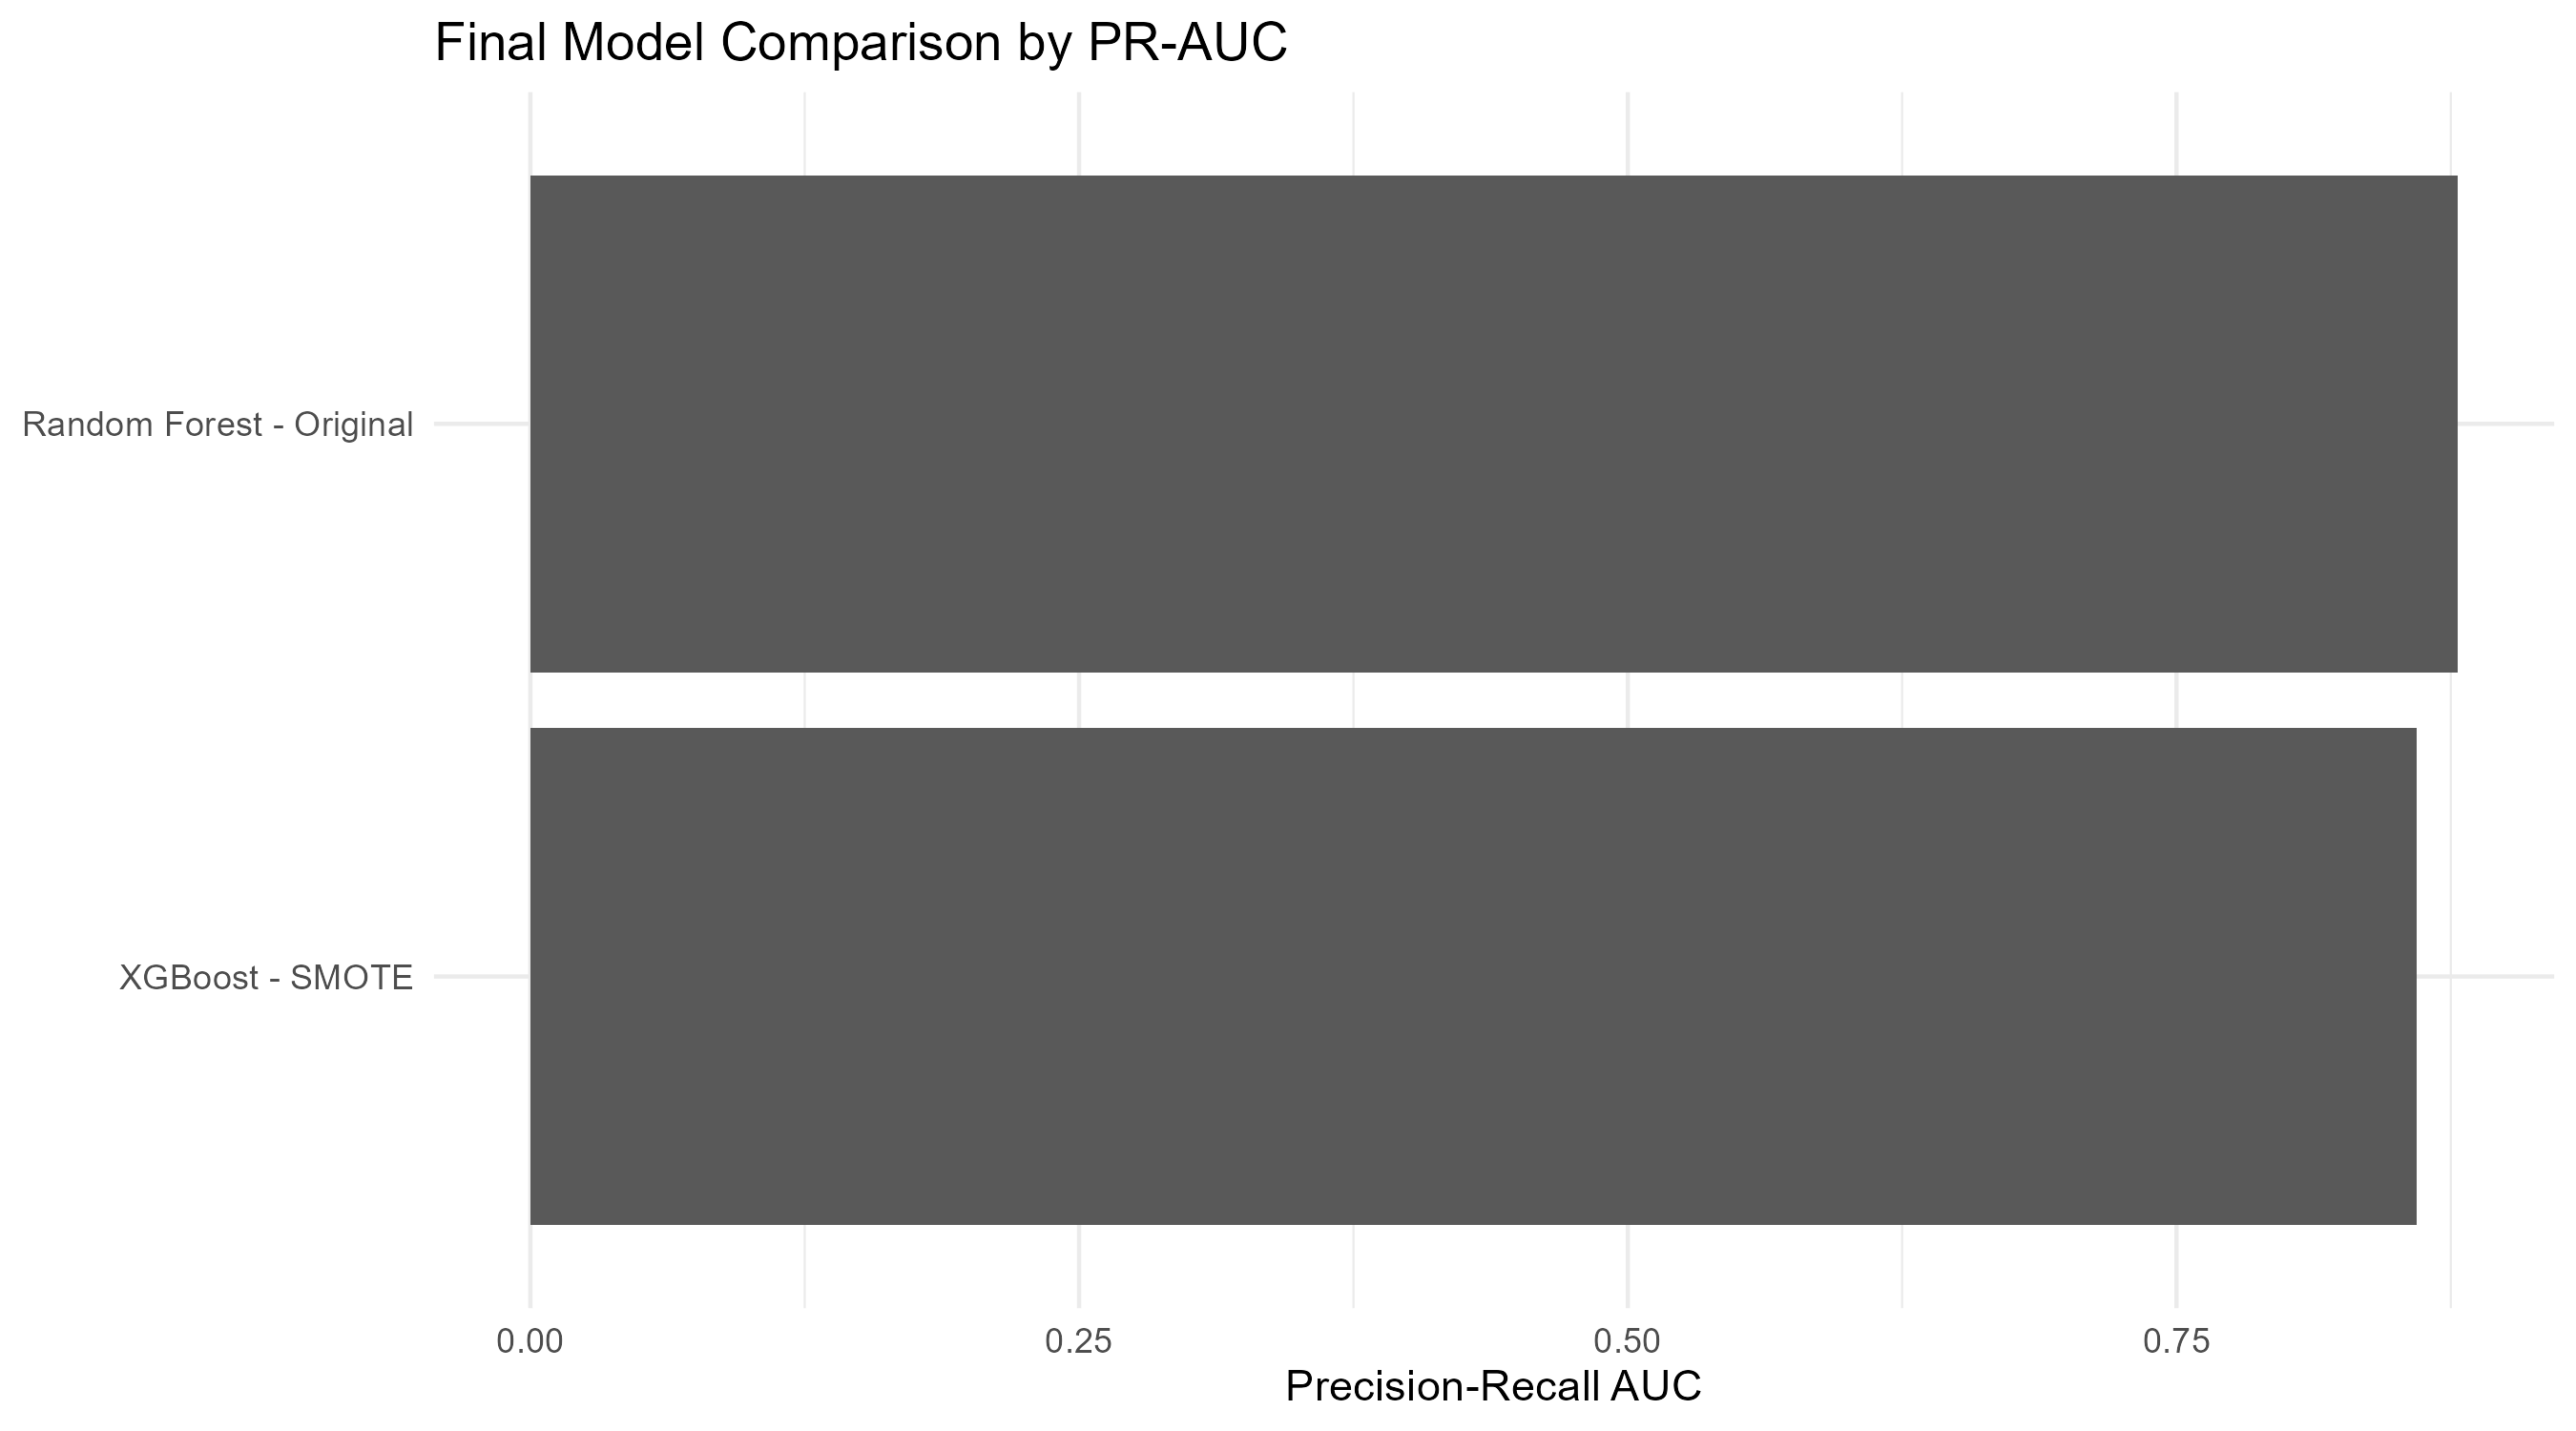
\includegraphics[keepaspectratio]{2-retail-analytics/../notebooks-and-scripts/2-retail-analytics/1-credit-card-fraud-detection-ml-benchmark/r/1-credit-card-fraud-detection-supervised-figures/final-model-comparison-pr-auc.png}}

}

\caption{\label{fig-final-model-comparison-pr-auc}Final model comparison
by Precision-Recall AUC.}

\end{figure}%

The confusion matrices in Figure~\ref{fig-confusion-matrices} show the
same trade-off from an operational perspective. Random Forest produces
fewer false positives, while XGBoost with SMOTE detects slightly more
fraudulent cases at the default threshold. This is the kind of result
where the ``best'' model depends less on the leaderboard and more on the
business rule attached to the score.

\begin{figure}

\centering{

\pandocbounded{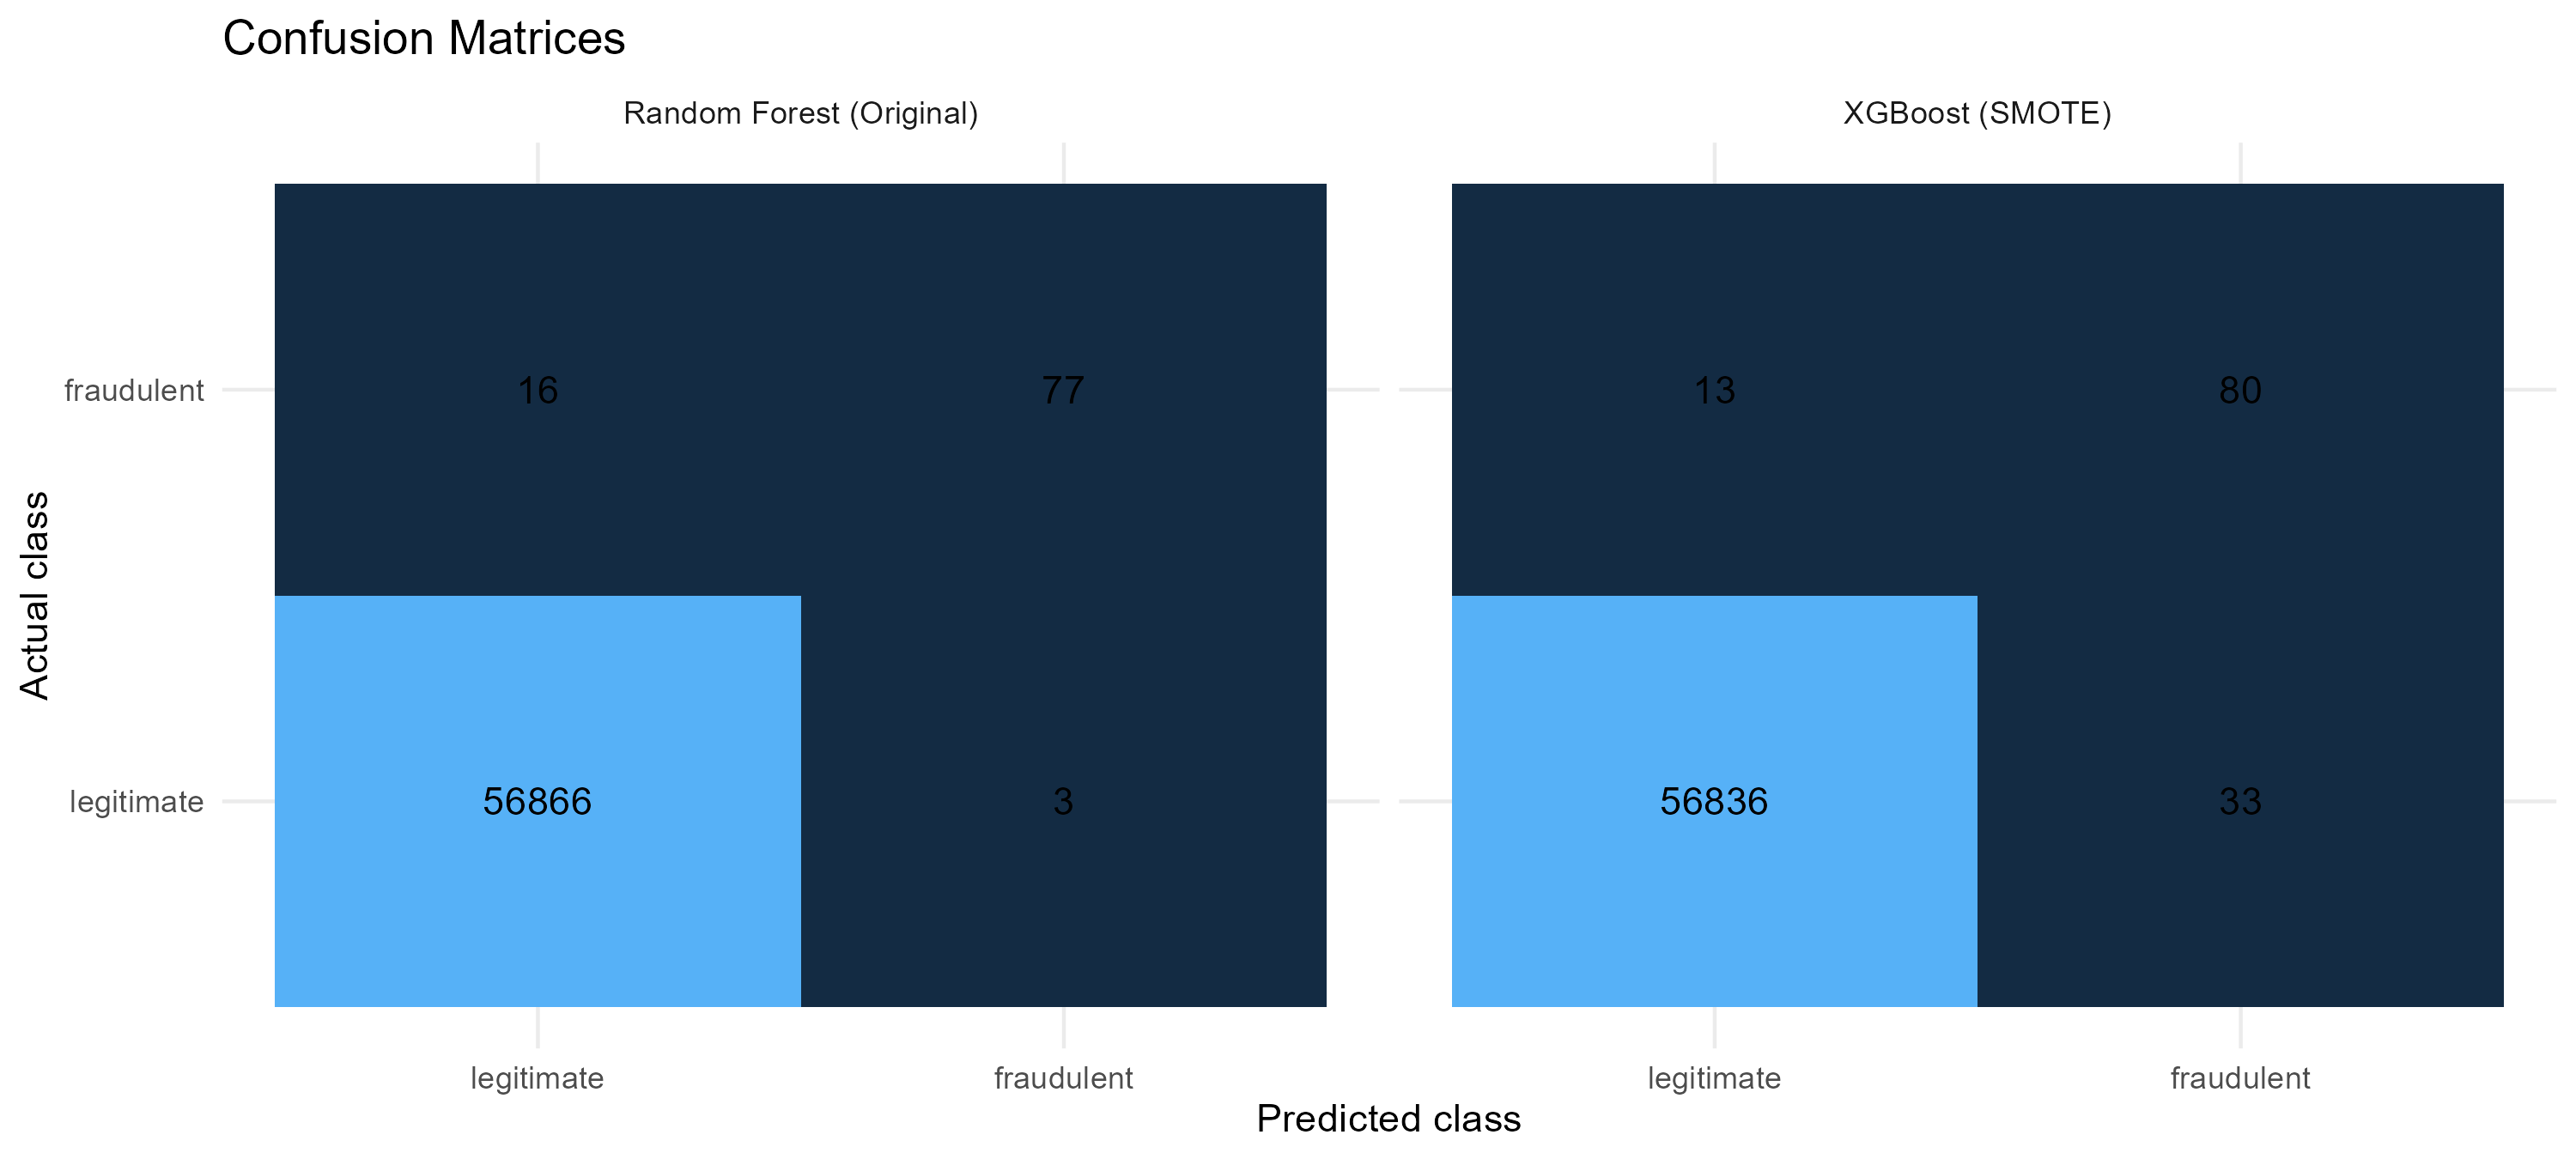
\includegraphics[keepaspectratio]{2-retail-analytics/../notebooks-and-scripts/2-retail-analytics/1-credit-card-fraud-detection-ml-benchmark/r/1-credit-card-fraud-detection-supervised-figures/confusion-matrices.png}}

}

\caption{\label{fig-confusion-matrices}Confusion matrices for the
retained supervised models.}

\end{figure}%

The ROC curves in Figure~\ref{fig-roc-curves} show that both models have
strong ranking ability across classification thresholds. XGBoost with
SMOTE has the higher ROC-AUC, which is consistent with its stronger
recall. However, ROC curves should be read carefully in this problem
because the number of legitimate transactions is so large that a small
false positive rate can still translate into many legitimate
transactions being flagged.

\begin{figure}

\centering{

\pandocbounded{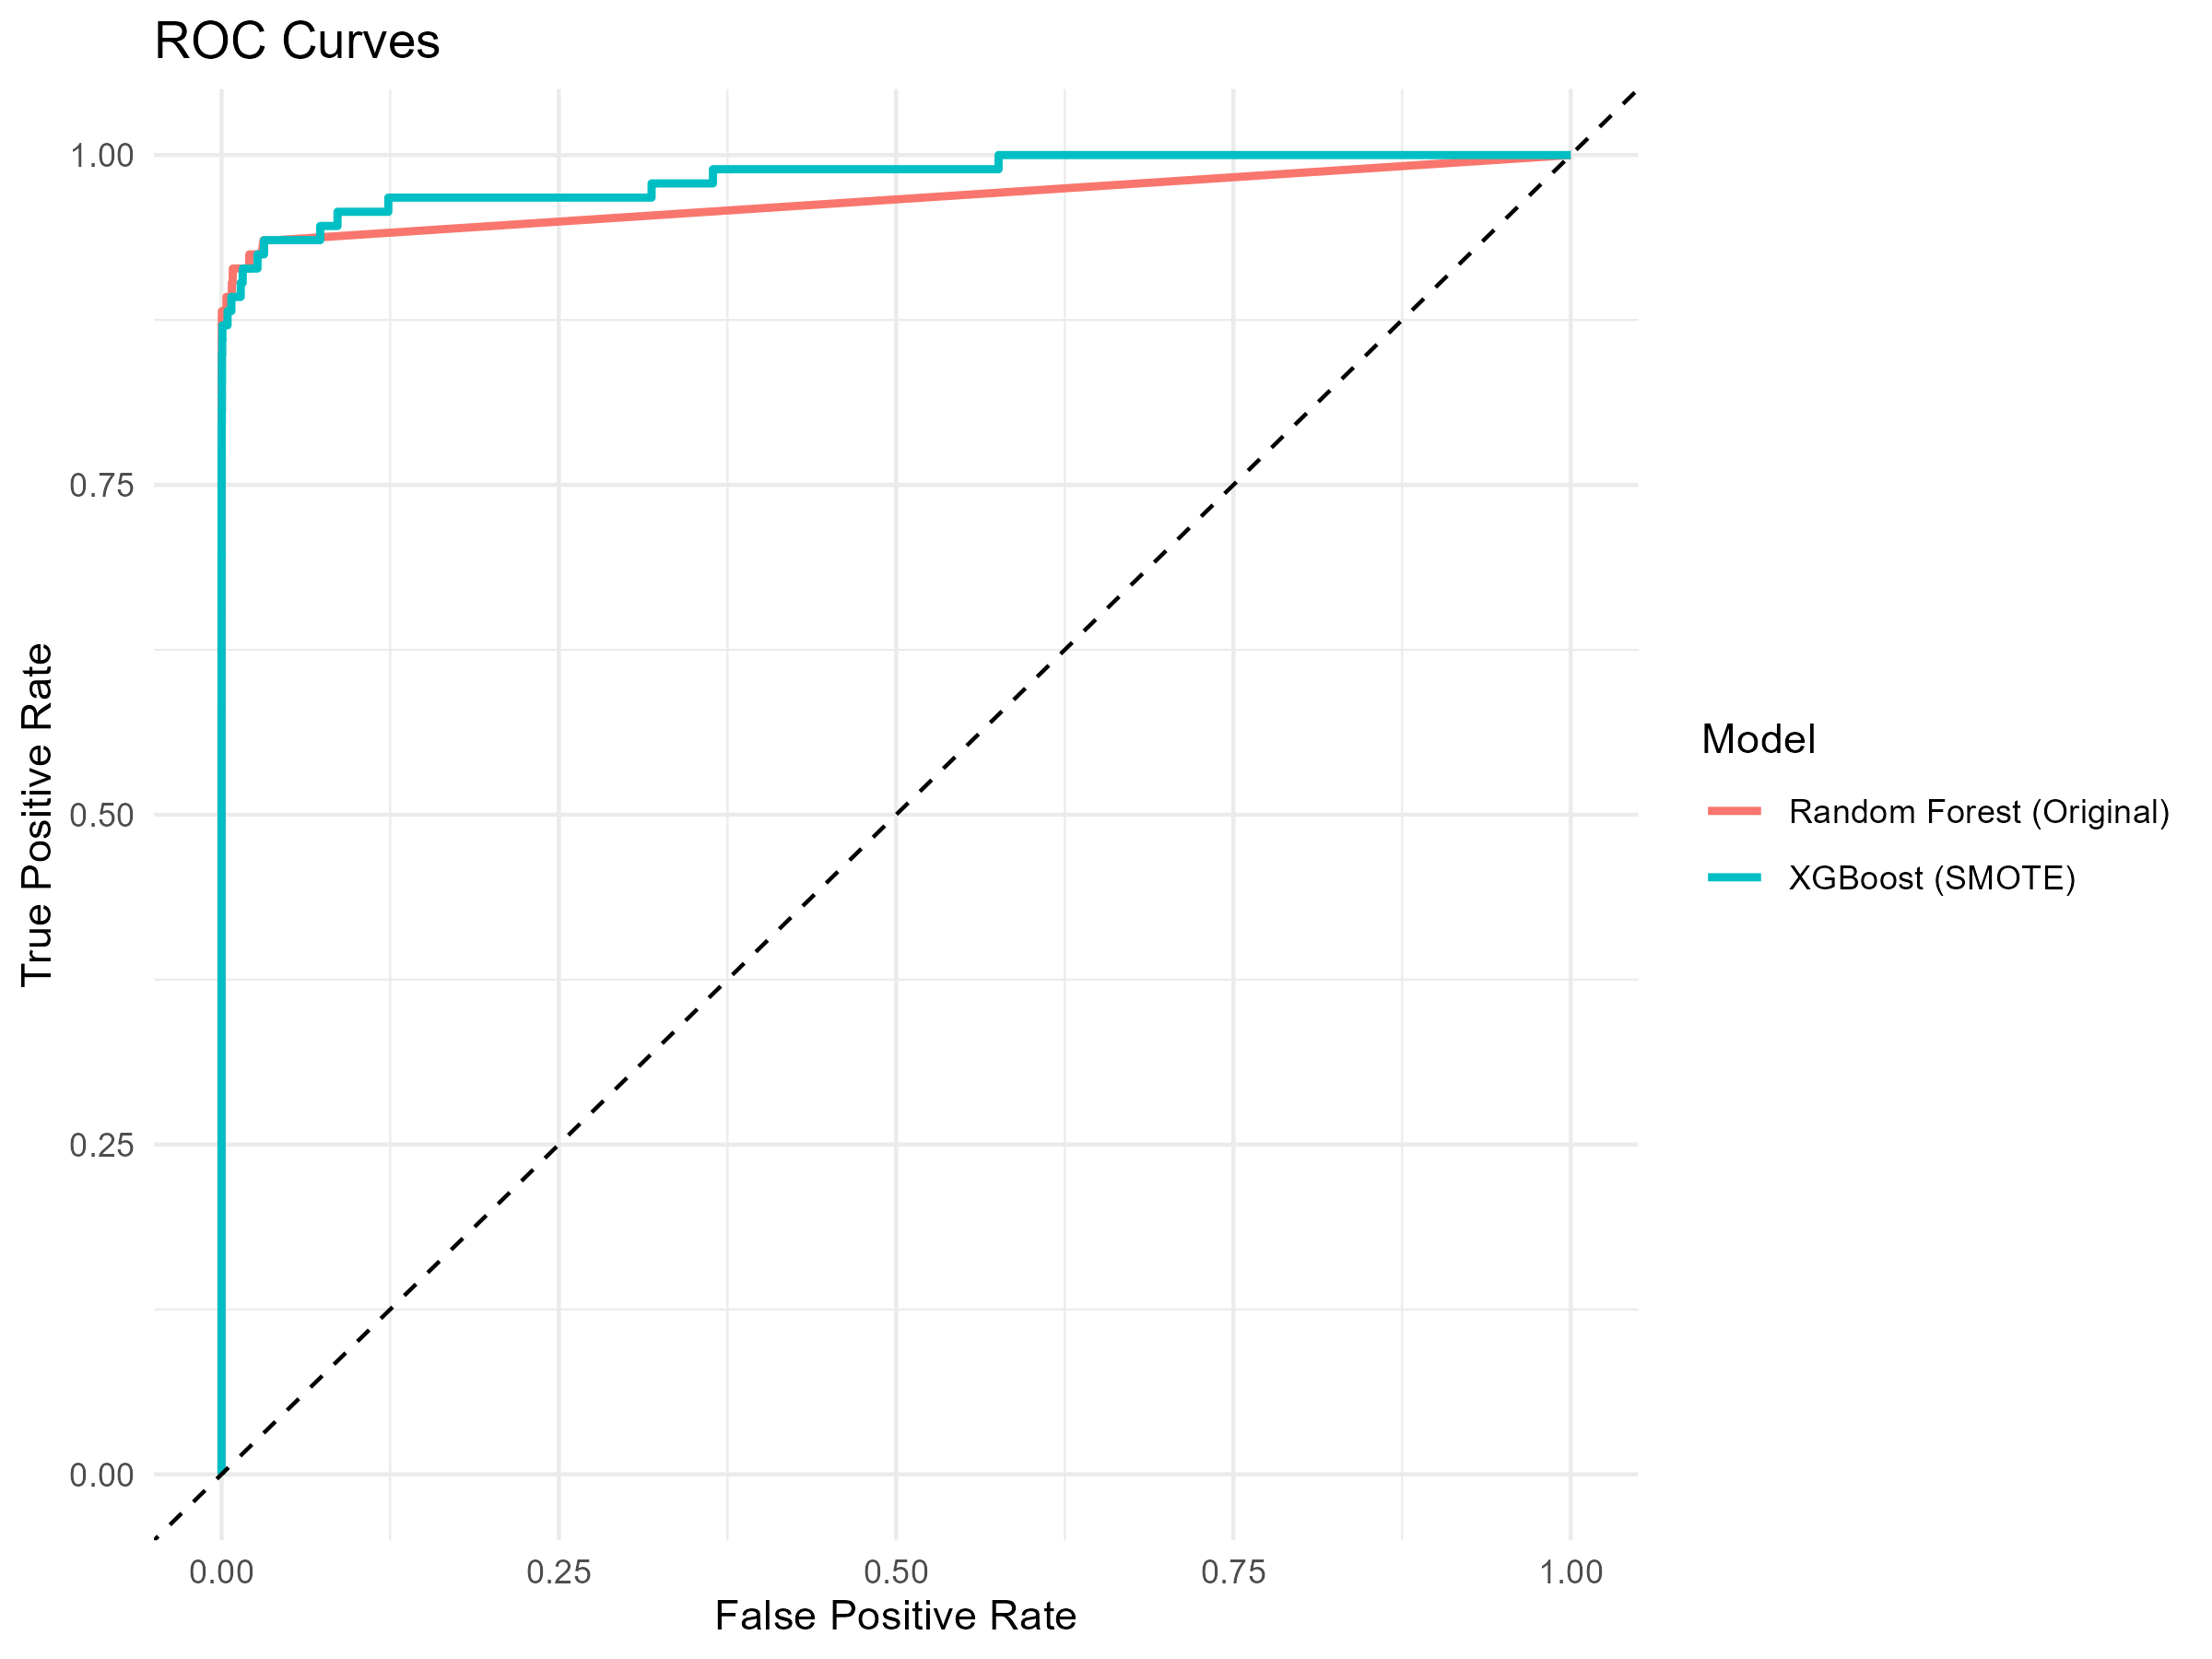
\includegraphics[keepaspectratio]{2-retail-analytics/../notebooks-and-scripts/2-retail-analytics/1-credit-card-fraud-detection-ml-benchmark/r/1-credit-card-fraud-detection-supervised-figures/roc-curves.png}}

}

\caption{\label{fig-roc-curves}ROC curves for the retained supervised
models.}

\end{figure}%

The Precision-Recall curves in Figure~\ref{fig-precision-recall-curves}
provide a more direct view of rare-class performance. They show how
precision changes as recall increases, which is often closer to the
decision that a fraud team needs to make: how many alerts can be
reviewed, and how many missed frauds are acceptable?

\begin{figure}

\centering{

\pandocbounded{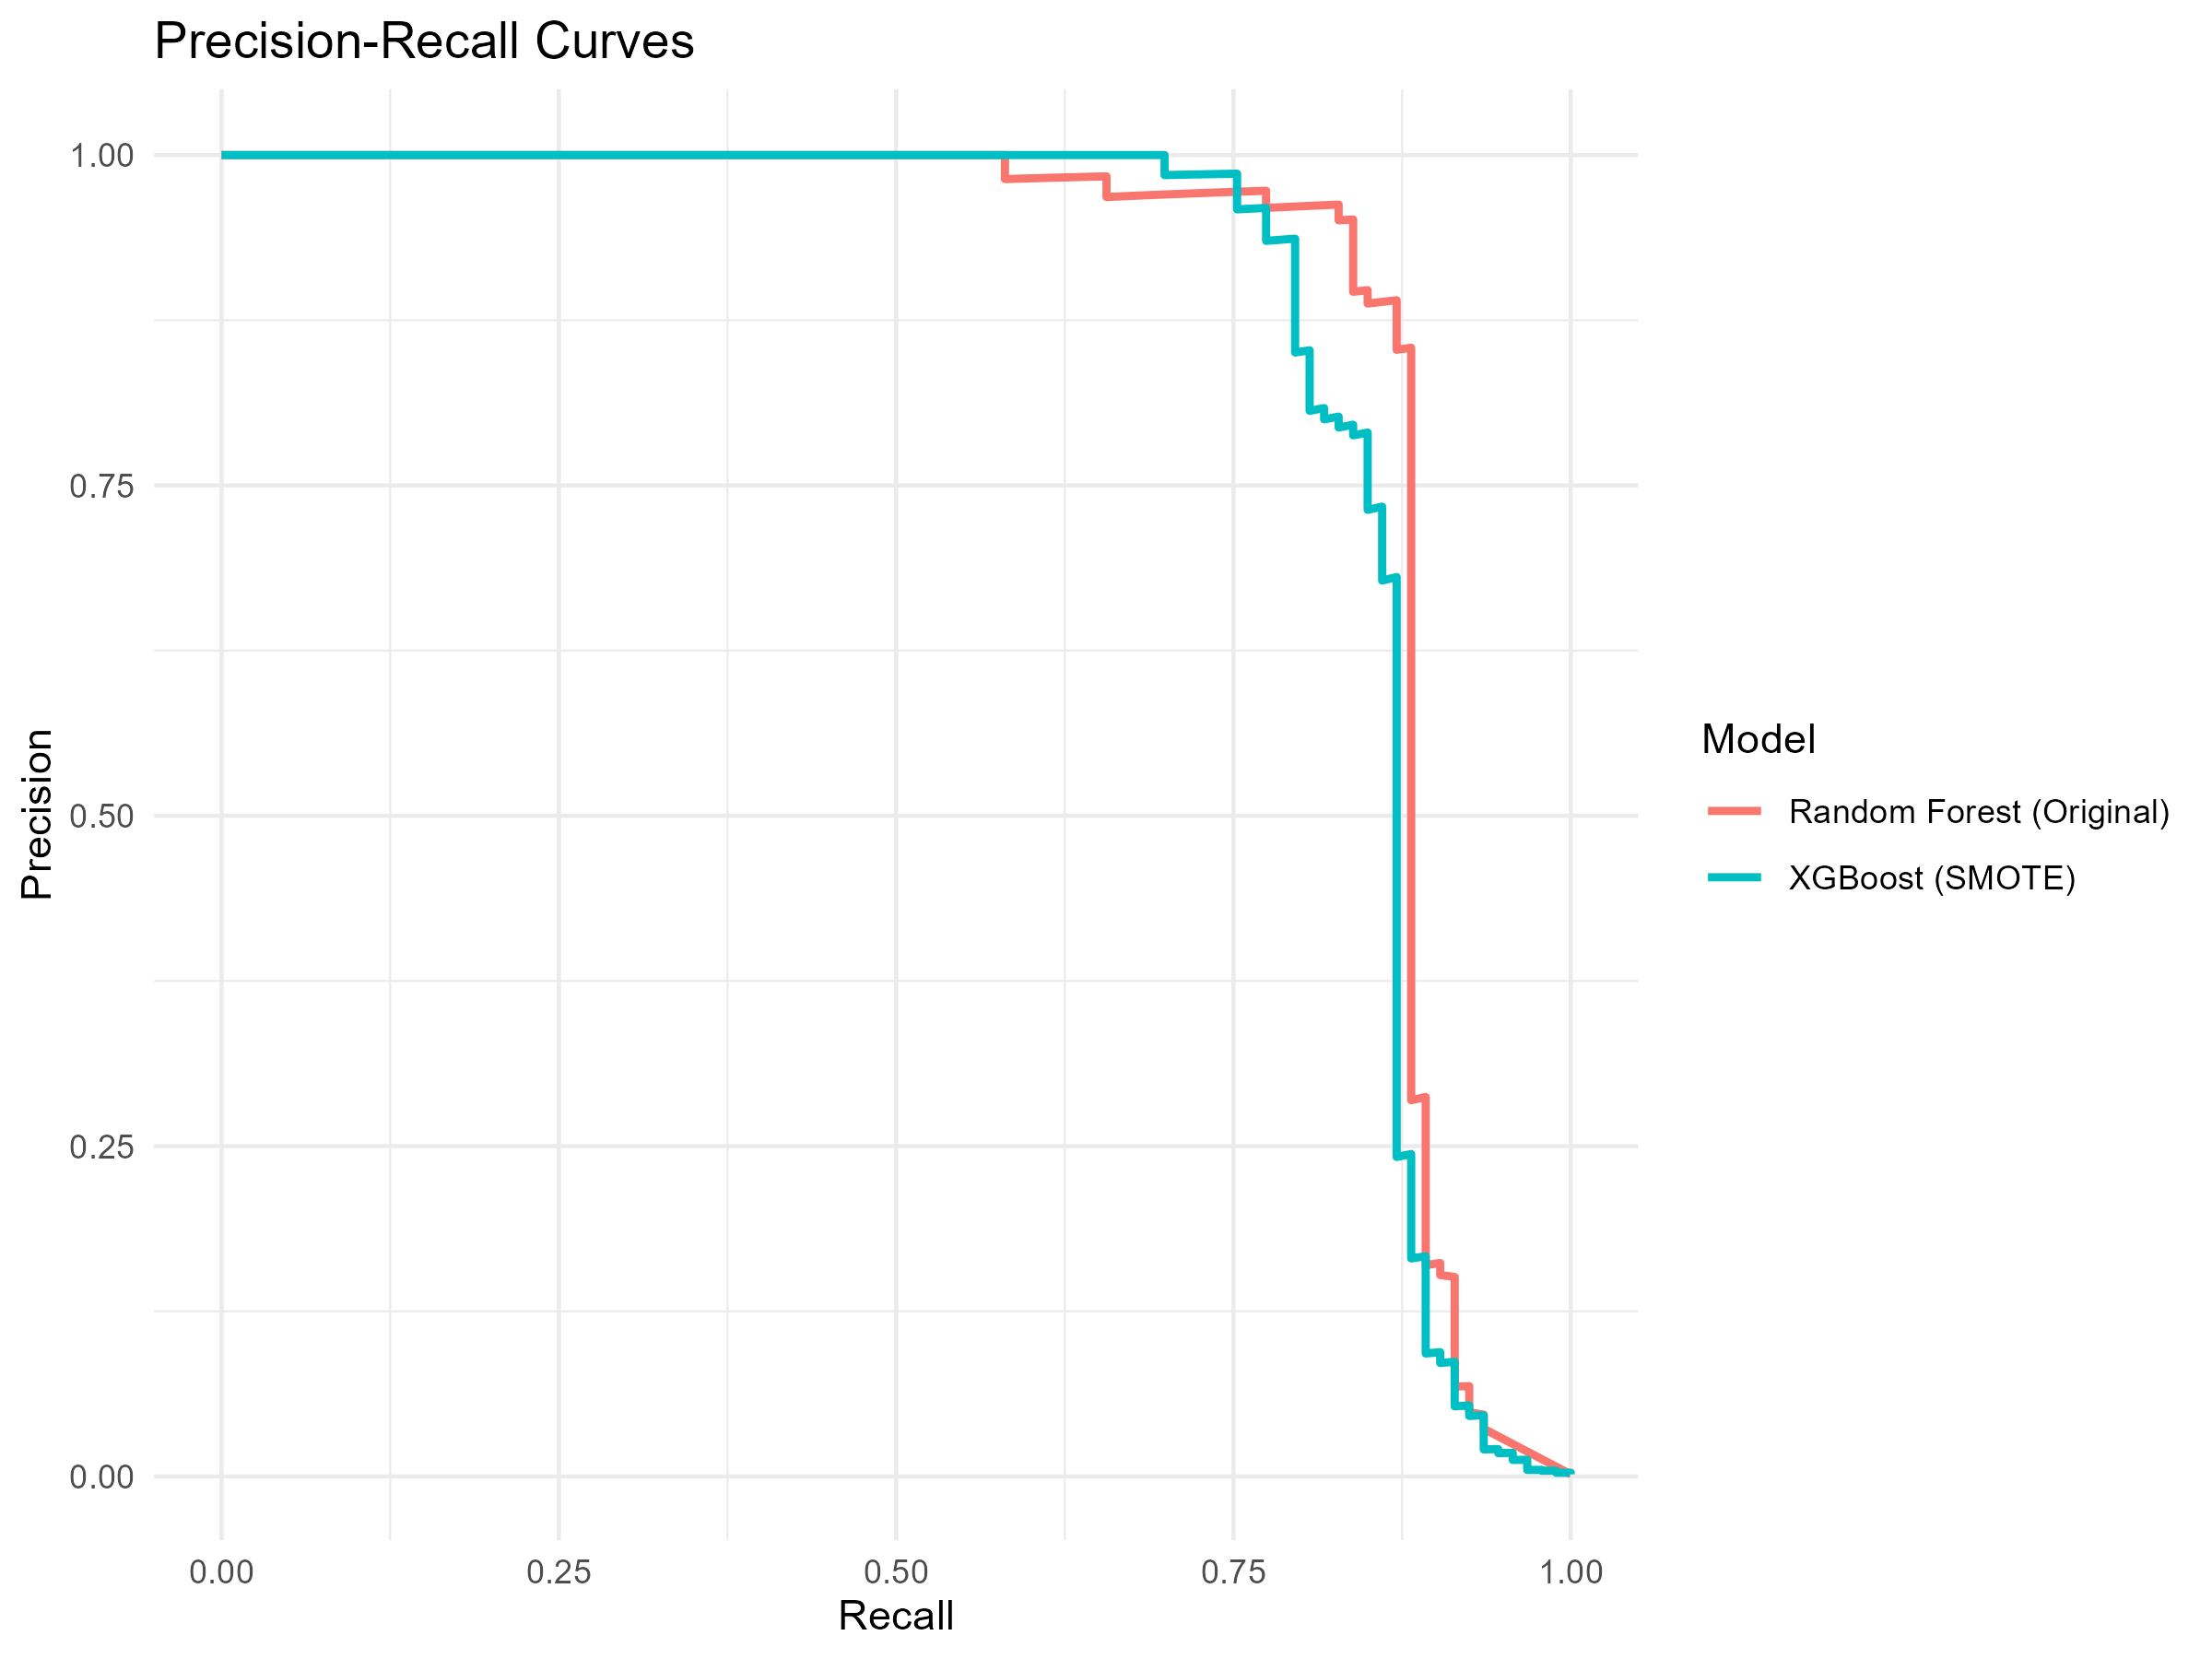
\includegraphics[keepaspectratio]{2-retail-analytics/../notebooks-and-scripts/2-retail-analytics/1-credit-card-fraud-detection-ml-benchmark/r/1-credit-card-fraud-detection-supervised-figures/precision-recall-curves.png}}

}

\caption{\label{fig-precision-recall-curves}Precision-Recall curves for
the retained supervised models.}

\end{figure}%

The KS statistic provides another way to assess whether the model scores
separate legitimate and fraudulent transactions. The values in
Table~\ref{tbl-kolmogorov-smirnov-statistic} are almost identical for
the two retained models.

\begin{longtable}[]{@{}cc@{}}
\caption{Kolmogorov-Smirnov statistic for the retained supervised
models.}\label{tbl-kolmogorov-smirnov-statistic}\tabularnewline
\toprule\noalign{}
Model strategy & KS statistic \\
\midrule\noalign{}
\endfirsthead
\toprule\noalign{}
Model strategy & KS statistic \\
\midrule\noalign{}
\endhead
\bottomrule\noalign{}
\endlastfoot
Random Forest - Original & 0.9056 \\
XGBoost - SMOTE & 0.9040 \\
\end{longtable}

The diagnostic plot in
Figure~\ref{fig-kolmogorov-smirnov-diagnostic-plot} shows the empirical
cumulative distributions of the predicted fraud probabilities for the
two classes. A wider separation between the curves indicates stronger
discrimination. The near-identical KS values suggest that both models
assign noticeably different score distributions to legitimate and
fraudulent transactions, even though their default-threshold behaviour
differs.

\begin{figure}

\centering{

\pandocbounded{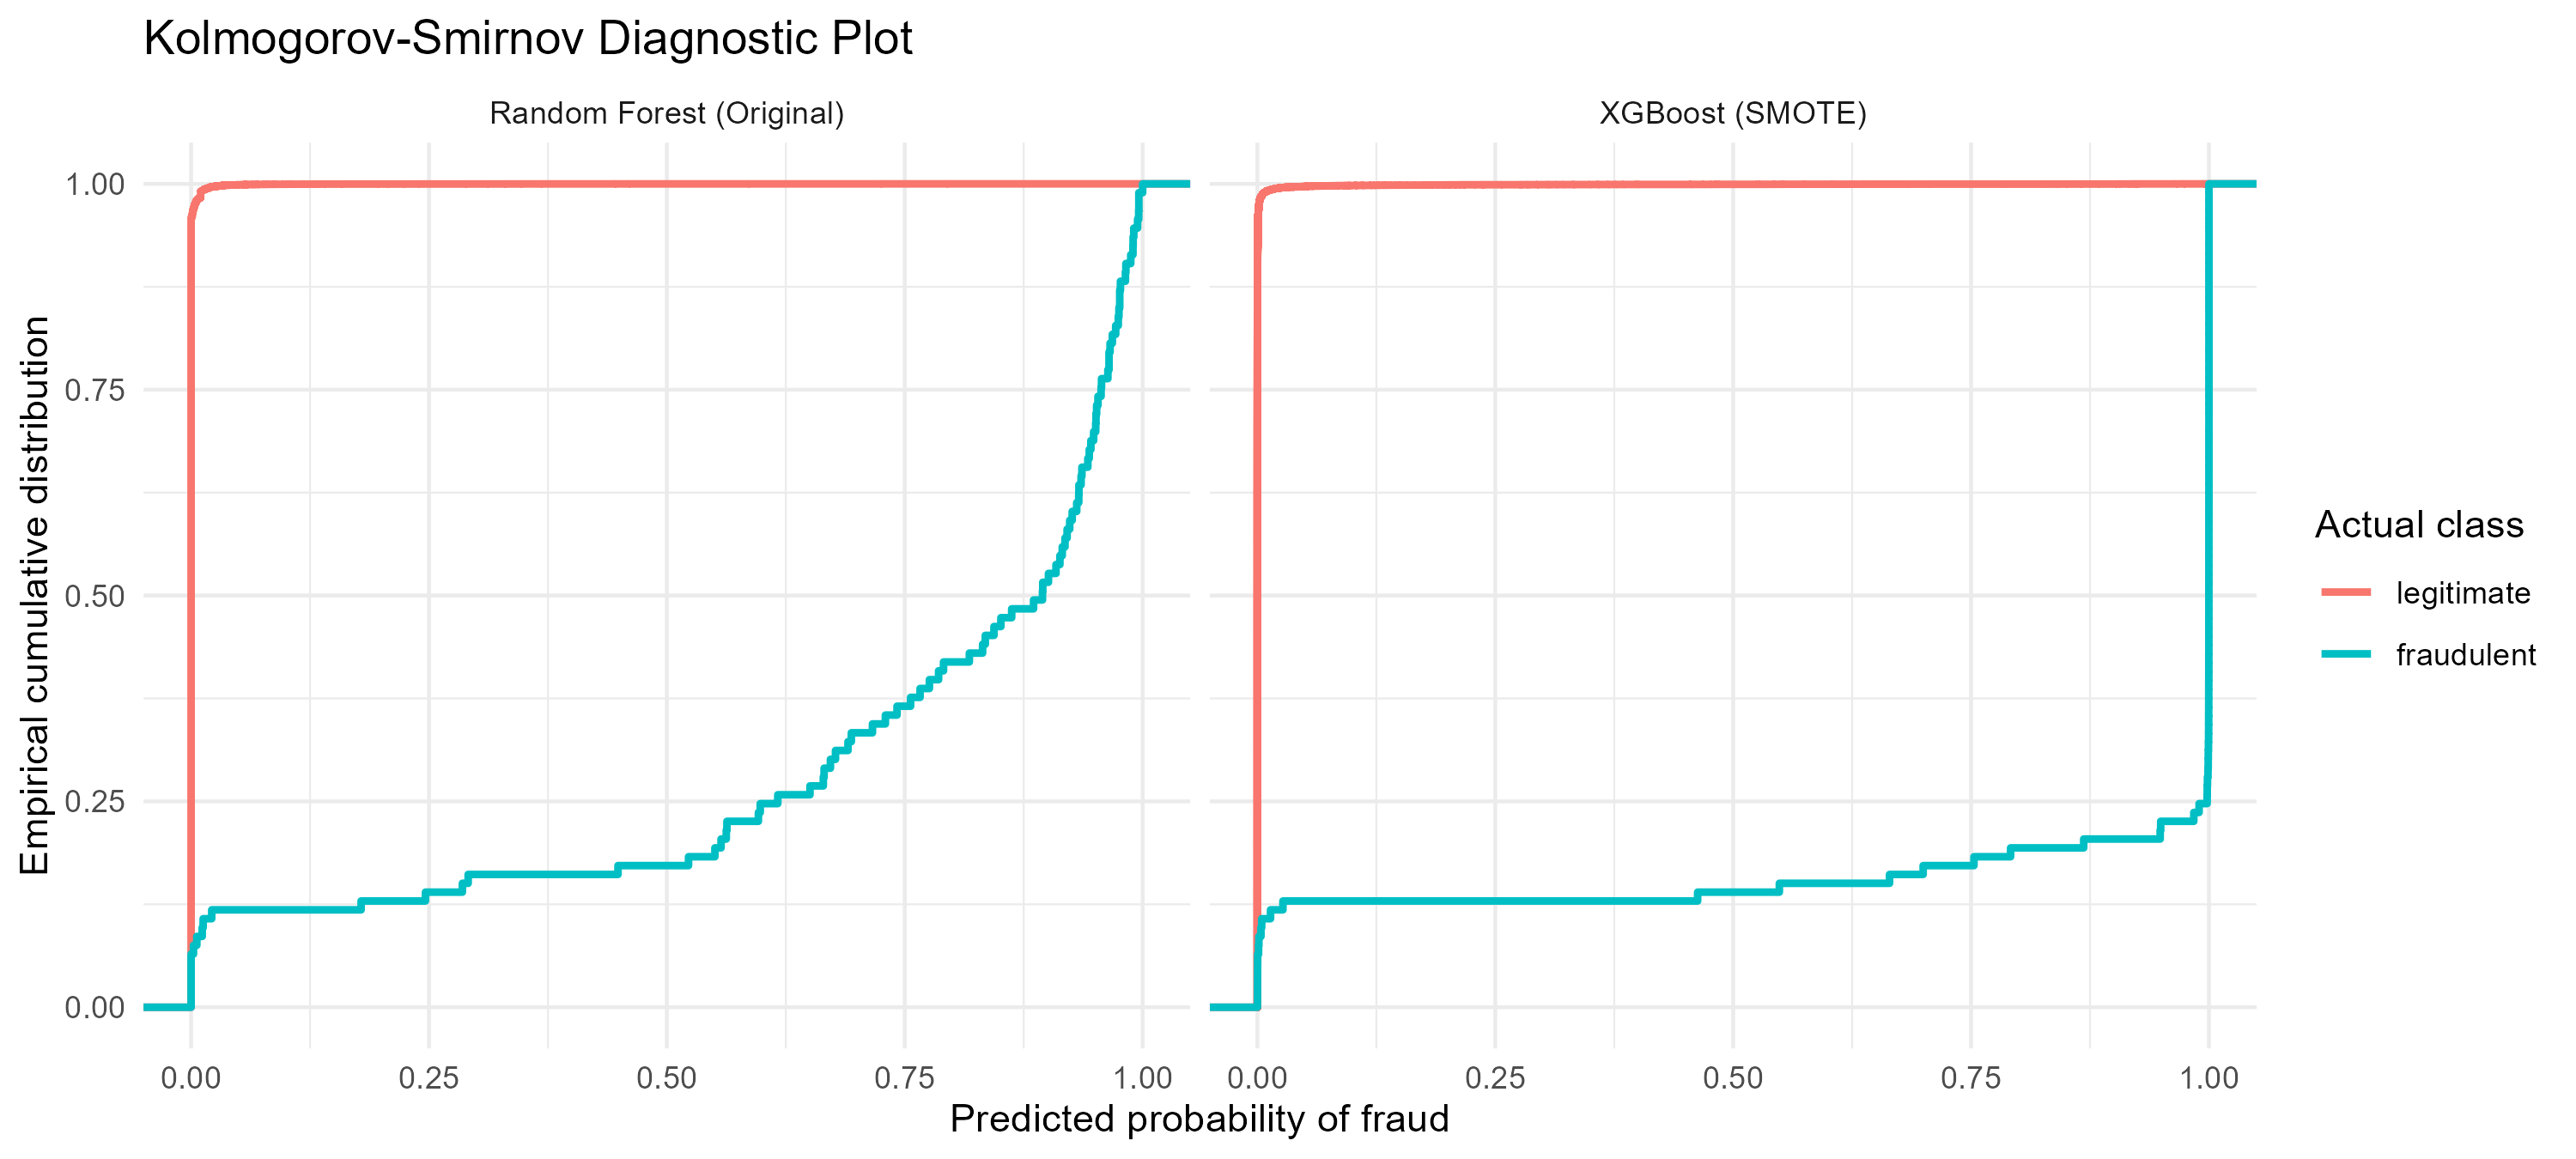
\includegraphics[keepaspectratio]{2-retail-analytics/../notebooks-and-scripts/2-retail-analytics/1-credit-card-fraud-detection-ml-benchmark/r/1-credit-card-fraud-detection-supervised-figures/kolmogorov-smirnov-diagnostic-plot.png}}

}

\caption{\label{fig-kolmogorov-smirnov-diagnostic-plot}Kolmogorov-Smirnov
diagnostic plot for the retained supervised models.}

\end{figure}%

From a modelling point of view, the main conclusion is that tree-based
ensemble methods are well suited to this dataset. They can capture
nonlinear relationships among the anonymized PCA features without
requiring a large amount of manual feature engineering. The original
Random Forest is a strong and stable option, while SMOTE makes XGBoost
more sensitive to fraudulent transactions. The stronger choice depends
on the preferred operating point. For a portfolio project aimed at a
practical analytics audience, this is an important distinction: the
model is not simply selected because it has the largest headline score,
but because its error profile fits the decision context.

Additional implementation details, including the companion Quarto and
Python notebooks, are available in the project repository
\href{https://github.com/rodrigokang/portfolio/tree/main/notebooks-and-scripts/2-retail-analytics/1-credit-card-fraud-detection-ml-benchmark}{\faGithub}

\section{Results, Discussion, and
Limitations}\label{results-discussion-and-limitations-3}

The benchmark highlights two consistent findings. First, tree-based
ensemble methods provided the most reliable discrimination between
legitimate and fraudulent transactions. Second, explicitly addressing
the class imbalance produced substantial improvements across almost
every classifier.

Random Forest and XGBoost achieved the strongest overall performance
because both algorithms are well suited to heterogeneous tabular data
containing complex, nonlinear relationships. Rather than relying on a
single global decision boundary, they partition the predictor space into
many local decision rules, allowing subtle interactions among the
anonymized variables to be captured. This flexibility is particularly
valuable in fraud detection, where fraudulent transactions rarely follow
a single, easily separable pattern.

The severe class imbalance proved to be the central modelling challenge.
With fraudulent transactions representing less than 0.2\% of the
observations, models trained on the original data naturally favored the
majority class. Under these conditions, high overall accuracy can be
achieved while missing a substantial fraction of fraudulent operations,
making accuracy a poor indicator of practical performance.

Applying resampling strategies before training shifted the learning
process toward the minority class. Random oversampling increased the
exposure of fraudulent examples, while SMOTE generated additional
synthetic observations that expanded the minority decision region
instead of simply duplicating existing cases. Although the magnitude of
the improvement varied across algorithms, the overall effect was
consistent: recall increased markedly, while precision typically
declined because more legitimate transactions were classified as
suspicious.

This trade-off between precision and recall is unavoidable in
operational fraud detection. A model optimized for precision reduces the
number of false alarms but may fail to detect fraudulent transactions. A
model optimized for recall identifies a larger proportion of fraud at
the expense of investigating more legitimate payments. The preferred
operating point ultimately depends on business costs, including the
financial impact of missed fraud, investigation capacity, customer
experience, and regulatory considerations.

For this reason, the Precision-Recall AUC provides a more informative
summary than the traditional ROC AUC. When the positive class is
extremely rare, ROC curves may appear optimistic because the false
positive rate changes only slightly even after many legitimate
transactions are incorrectly flagged. Precision-Recall curves focus
exclusively on the minority class by evaluating how many detected alerts
are actually fraudulent and how many fraudulent transactions are
successfully recovered. As a result, they offer a more realistic
assessment of model quality under extreme class imbalance.

Several limitations should be considered when interpreting these
results. The predictors available in the public dataset were anonymized
through Principal Component Analysis before release, preventing any
interpretation of which original transaction characteristics contributed
most to the predictions. The analysis also relies on a single historical
collection of European card transactions observed over a limited time
window. Fraud patterns evolve continuously as attackers adapt to
existing detection systems, meaning that a model calibrated on
historical behaviour may gradually lose predictive power through concept
drift. In practice, production systems require continuous monitoring,
periodic recalibration of decision thresholds, and regular retraining as
new labelled transactions become available. Consequently, the benchmark
should be viewed as a comparison of modelling strategies under
controlled conditions rather than as a final fraud detection system
ready for deployment.

\section{Technical Appendix}\label{technical-appendix}

This appendix summarizes the methodological concepts required to
understand the modelling decisions presented in the benchmark. The
objective is to provide enough theoretical background to interpret the
results without developing the algorithms in full mathematical detail.

\subsection{Random Forest}\label{random-forest}

Random Forest is an ensemble learning algorithm that combines the
predictions of many decision trees. Rather than relying on a single
tree, the model aggregates a collection of independently constructed
trees, producing predictions that are typically more stable and less
sensitive to random fluctuations in the training data.

\subsubsection{Decision Trees}\label{decision-trees}

A decision tree partitions the predictor space into a sequence of
increasingly homogeneous regions. Starting from the root node, the
algorithm repeatedly selects the feature and split point that best
separate the observations according to a chosen impurity criterion. The
final leaves contain observations with similar characteristics, and each
leaf is assigned a class probability based on the proportion of
fraudulent transactions it contains.

For a binary classification problem, the estimated probability of fraud
at a terminal node is simply

\begin{equation}\phantomsection\label{eq-rf-probability}{
\hat{p}=\frac{\text{Number of fraudulent observations}}{\text{Total observations in the node}}.
}\end{equation}

Although decision trees are easy to interpret and naturally capture
nonlinear relationships and feature interactions, a single tree is
usually unstable. Small changes in the training data may produce
substantially different tree structures.

\subsubsection{Ensemble Prediction}\label{ensemble-prediction}

Random Forest addresses this instability by combining many trees built
from slightly different versions of the training data while also
considering random subsets of predictors at each split. The final
prediction is obtained through majority voting,

\begin{equation}\phantomsection\label{eq-rf-majority-vote}{
\hat{y}=\operatorname*{mode}\left(\hat{y}_1,\hat{y}_2,\ldots,\hat{y}_B\right),
}\end{equation}

where \(\hat{y}_b\) denotes the prediction of the \(b\)-th tree.

Class probabilities are estimated by averaging the probabilities
produced by the individual trees,

\begin{equation}\phantomsection\label{eq-rf-probability-ensemble}{
\hat{P}(y=1\mid x)=\frac{1}{B}\sum_{b=1}^{B}\hat{P}_b(y=1\mid x).
}\end{equation}

Because prediction is based on many independent trees rather than a
single model, Random Forest generally achieves lower variance and better
generalization. These characteristics explain why it consistently
performs well on structured tabular datasets such as credit card
transaction records. Its main limitations are reduced interpretability
compared with a single decision tree and larger computational
requirements as the number of trees increases.

\subsection{XGBoost}\label{xgboost}

XGBoost is an optimized implementation of Gradient Boosting in which
trees are added sequentially instead of independently. Each new tree is
trained to reduce the prediction errors made by the ensemble constructed
so far, allowing the model to progressively refine its representation of
complex decision boundaries.

If the prediction after \(t-1\) trees is \(\hat{y}^{(t-1)}\), the next
tree contributes a correction,

\begin{equation}\phantomsection\label{eq-xgb-additive-model}{
\hat{y}^{(t)}=\hat{y}^{(t-1)}+f_t(x),
}\end{equation}

where \(f_t\) represents the new decision tree.

Rather than minimizing only the training loss, XGBoost optimizes a
regularized objective function,

\begin{equation}\phantomsection\label{eq-xgb-objective}{
\mathcal{L}=\sum_{i=1}^{n}l(y_i,\hat{y}_i)+\sum_{t}\Omega(f_t),
}\end{equation}

where \(l(\cdot)\) measures the prediction error and \(\Omega(\cdot)\)
penalizes overly complex trees.

The regularization term discourages unnecessarily deep or highly
specialized trees, reducing the risk of overfitting while preserving
predictive accuracy. Together with efficient optimization procedures and
effective handling of nonlinear feature interactions, this design
explains why XGBoost frequently ranks among the strongest performers on
structured tabular datasets.

\subsection{Handling Class Imbalance}\label{handling-class-imbalance}

Fraud detection datasets are naturally imbalanced because fraudulent
transactions represent only a very small fraction of all operations.
Standard classification algorithms are designed to minimize overall
prediction error, so they tend to prioritize the majority class unless
corrective measures are introduced during training.

One widely used approach is the Synthetic Minority Over-sampling
Technique (SMOTE). Instead of duplicating existing minority
observations, SMOTE generates new synthetic examples by interpolating
between neighboring fraudulent transactions in the feature space.

For each minority observation, the algorithm selects one of its nearest
minority neighbours and creates a synthetic sample along the line
joining the two observations,

\begin{equation}\phantomsection\label{eq-smote-synthetic-sample}{
x_{\mathrm{new}}=x_i+\lambda(x_j-x_i),
}\end{equation}

where \(x_i\) is an existing minority observation, \(x_j\) is one of its
nearest minority neighbours, and \(\lambda\in[0,1]\) is a random
interpolation factor.

By populating the minority region with plausible synthetic observations,
SMOTE encourages the classifier to learn broader decision boundaries
instead of focusing on a handful of isolated fraud cases. This generally
improves the ability to recover fraudulent transactions while avoiding
the excessive duplication that can occur with simple random
oversampling.

Several extensions combine synthetic oversampling with subsequent
cleaning procedures that remove ambiguous or overlapping observations
near the class boundary. Although such hybrid methods can further
improve performance in some applications, the benchmark presented in
this chapter focuses on the standard resampling strategies needed to
evaluate the effect of class imbalance on the candidate classifiers.

\chapter{Customer Value and
Retention}\label{customer-value-and-retention}

Customer relationships are among the most valuable assets of a business,
yet they are also among the most difficult to quantify. While
transactional databases record what customers have purchased, they
rarely explain how purchasing behaviour evolves over time or which
customers deserve the greatest commercial attention. As a result,
organisations often rely on simple indicators such as historical revenue
or purchase counts, even though these metrics provide only a partial
view of customer behaviour.

Database marketing has long recognised that effective customer
management requires combining behavioural analysis with predictive and
financial perspectives rather than relying on a single performance
indicator \citeproc{ref-robert2008database}{{[}29{]}}. Understanding who
customers are, who is likely to leave, and which relationships are
expected to generate the greatest long-term value are closely related
questions that should be addressed within a unified analytical
framework.

This chapter develops a complete customer analytics workflow for a
non-contractual retail business using transactional data from the
AdventureWorks database. Unlike subscription businesses, where customer
churn is explicitly observed through contract cancellations, retail
businesses rarely record when a customer relationship has ended.
Instead, customer behaviour must be inferred from historical purchasing
activity.

The analysis is organised around three complementary tasks. First,
customers are segmented using Recency, Frequency, and Monetary (RFM)
variables to identify groups with similar purchasing behaviour. Second,
churn is formulated as a supervised learning problem by defining
customer inactivity over a future observation window. Finally, customer
lifetime value (CLV) is estimated by combining customer profitability
with retention risk and explicit discount-rate assumptions.

Rather than presenting these models as independent analyses, the chapter
demonstrates how descriptive analytics, predictive modelling, and
economic valuation can be integrated into a single decision-support
workflow. The emphasis is not on producing a universal customer score,
but on developing a transparent framework in which every modelling
assumption remains explicit and interpretable.

\section{Problem Definition}\label{problem-definition-4}

Customer value is inherently difficult to assess in a non-contractual
business. Unlike subscription services, where customers can be
classified as active or cancelled, retail customers may purchase
irregularly, return after long periods of inactivity, or buy only
seasonally. Consequently, the absence of recent transactions does not
necessarily indicate that a customer has churned.

This uncertainty complicates several common business decisions. Which
customers should receive retention efforts? Which customers appear
valuable but are gradually becoming inactive? Which recently acquired
customers show early signs of future growth? Which inactive customers
are unlikely to return?

Historical revenue alone cannot answer these questions because it
ignores how recently customers have purchased, how frequently they buy,
and how likely they are to continue purchasing in the future. Likewise,
prioritising customers solely according to churn probability overlooks
the fact that not every customer contributes equally to the business.

The AdventureWorks database provides a realistic environment for
studying these problems because it stores detailed transactional
information across customers, orders, products, costs, and sales
territories. Rather than relying on pre-computed customer summaries,
this project reconstructs customer behaviour directly from transactional
records and derives the features required for segmentation, churn
prediction, and customer value estimation.

The analysis therefore addresses three related questions.

\begin{itemize}
\tightlist
\item
  How can customers be grouped according to their purchasing behaviour?
\item
  Which customers appear most likely to become inactive?
\item
  How does expected customer value change once profitability, retention
  risk, and discounting are considered simultaneously?
\end{itemize}

Although each question can be investigated independently, combining them
provides a substantially richer understanding of customer relationships
than any single model alone.

\section{Modeling Approach}\label{modeling-approach-4}

The analytical workflow follows a layered structure in which each stage
provides information for the next.

The first stage focuses on behavioural segmentation. Customer-level RFM
variables are computed from the complete transaction history available
for each individual. Because these variables exhibit strong positive
skewness, they are transformed and standardised before applying K-Means
clustering. The resulting clusters are then interpreted using the
original RFM variables to preserve their business meaning.

The second stage introduces prediction through churn modelling. Since
customer churn is not explicitly recorded in the AdventureWorks
database, an operational target is constructed by separating the
available transaction history into calibration and observation periods.
Customers who make no purchases during the observation window are
labelled as churned, allowing the problem to be formulated as a
supervised classification task while avoiding information leakage.

The final stage estimates customer lifetime value. Customer
profitability is derived from historical revenue and product costs,
while segment-specific retention behaviour and discount-rate assumptions
are used to construct a risk-adjusted valuation framework. A regression
model is then trained to approximate this valuation using the
customer-level features engineered throughout the previous stages.

Viewed as a whole, the workflow progresses naturally from behavioural
description to future risk estimation and finally to economic value.
Rather than producing isolated analytical models, each stage complements
the previous one, resulting in a coherent framework for customer
prioritisation and retention planning.

\section{Methodology and
Implementation}\label{methodology-and-implementation-4}

The methodology is organised into three complementary stages that
progressively transform transactional sales records into actionable
customer insights. Although each stage addresses a different analytical
problem, they are connected through a common customer-level feature
engineering pipeline built from the AdventureWorks transactional
database.

The workflow begins by describing customer purchasing behaviour through
RFM segmentation. These behavioural profiles then provide additional
context for a supervised churn prediction model, where customer
inactivity is defined using future purchasing behaviour observed within
a separate validation period. Finally, the outputs of the previous
stages are combined with profitability information to construct a
risk-adjusted Customer Lifetime Value (CLV) framework that supports
customer prioritisation from both behavioural and financial
perspectives.

Rather than treating segmentation, churn prediction, and lifetime value
estimation as independent modelling exercises, the implementation
integrates them into a single analytical workflow in which each stage
provides information that strengthens the interpretation of the next.

\subsection{Customer Segmentation with RFM
Analysis}\label{customer-segmentation-with-rfm-analysis}

Customer segmentation provides the behavioural foundation for the
remainder of the chapter. Instead of analysing thousands of customers
individually, the objective is to identify groups with similar
purchasing patterns that can later support both churn prediction and
customer value estimation.

The implementation begins by extracting transaction-level data directly
from the AdventureWorks database rather than relying on pre-aggregated
customer tables. Sales orders, order details, products, product
categories, customers, and sales territories are combined to create a
reusable transactional dataset from which customer-level features can be
derived consistently throughout the project.

Customer behaviour is summarised using the classical Recency, Frequency,
and Monetary (RFM) framework. Recency measures the time elapsed since
the customer's most recent purchase, Frequency counts completed purchase
events, and Monetary represents cumulative customer spending over the
observation period. Because these variables exhibit strong positive
skewness, particularly Frequency and Monetary value, they are
transformed using the Box-Cox transformation and standardised before
clustering to reduce the influence of extreme observations.

Customer segments are then identified using the K-Means algorithm.
Rather than selecting the number of clusters arbitrarily, several
candidate solutions are evaluated using complementary internal
validation metrics, including the silhouette coefficient, the
Calinski--Harabasz Index, and the Davies--Bouldin Index. The final
segmentation balances statistical quality with business
interpretability, allowing each cluster to be characterised according to
the original RFM variables rather than the transformed feature space.

To complement the discrete segmentation, the implementation also
introduces a continuous within-segment RFM score that ranks customers
according to their relative purchasing behaviour inside each cluster.
This additional layer helps distinguish customers who belong to the same
behavioural segment but differ in their overall commercial importance,
providing a practical prioritisation mechanism for subsequent retention
activities.

The resulting customer segments constitute the descriptive layer of the
analytical workflow and are subsequently incorporated as explanatory
variables in both the churn prediction and customer lifetime value
models.

The complete Python implementation of this workflow, including data
extraction, feature engineering, clustering diagnostics, segment
interpretation, and customer scoring, is available in the companion
notebook linked above.

A complete Python implementation of the RFM analysis presented in this
section is available in the project repository
\href{https://github.com/rodrigokang/portfolio/tree/main/notebooks-and-scripts/2-retail-analytics/2-customer-value-and-retention}{here}.

\subsection{Churn Prediction in Non-Contractual Relationships Based on
RFM
Analysis}\label{churn-prediction-in-non-contractual-relationships-based-on-rfm-analysis}

Once the customer segments have been established, the analysis shifts
from behavioural description to predictive modelling. The objective is
no longer to characterise purchasing behaviour, but to identify
customers who appear at risk of becoming inactive in the near future. In
a non-contractual retail environment, however, this is not
straightforward because the absence of recent purchases does not
necessarily imply that a customer has permanently left. Instead, churn
must be defined operationally from observed purchasing behaviour.

To reproduce a realistic prediction scenario, the available transaction
history is divided into calibration and observation periods. All
explanatory variables are computed exclusively from the calibration
window, while customer activity during the subsequent observation period
is used only to validate the churn outcome. This chronological
separation ensures that every predictor reflects information that would
have been available at the time the prediction was made, thereby
preventing information leakage.

Rather than defining churn solely as the absence of future purchases,
the implementation combines several behavioural indicators derived
during the calibration period. Customers are first identified as
potential churners if they belong to a low-activity behavioural segment,
their recency exceeds their historical average purchase latency, and
their within-segment RFM score falls below the average score of their
corresponding segment. These behavioural conditions identify customers
whose purchasing patterns are consistent with progressive disengagement
rather than temporary inactivity. A customer is ultimately labelled as
churned only if no additional purchases are observed during the
subsequent validation period. This two-stage definition combines
historical behaviour with future purchasing activity, producing a target
that remains consistent with the non-contractual nature of retail
customer relationships while avoiding information leakage.

The predictive feature set extends the variables developed during the
segmentation stage. In addition to the original RFM variables and
customer segment assignments, the implementation derives customer-level
descriptors that capture purchasing cadence, average order value,
customer tenure, product diversity, profitability, purchase intervals,
geographic information, and several aggregated transaction statistics.
Together, these variables provide a more comprehensive representation of
customer behaviour than RFM alone while preserving a clear business
interpretation.

Several supervised learning algorithms are evaluated under a common
modelling framework using cross-validation and hyperparameter
optimisation. Because churned customers represent only a minority of the
customer base, particular attention is given to model evaluation under
class imbalance. Performance is therefore assessed using complementary
metrics, including ROC AUC, Average Precision, Precision, Recall, and
F1-score. In addition, cumulative gains analysis is used to evaluate how
effectively customers can be ranked according to their estimated churn
risk, which is often more valuable for retention planning than binary
classification alone.

Rather than producing deterministic decisions, the selected classifier
estimates the probability that each customer will become inactive during
the observation period. These probabilities provide a practical ranking
of retention risk that can support targeted marketing campaigns,
customer prioritisation, and proactive retention strategies. They also
constitute one of the principal inputs for the risk-adjusted customer
lifetime value framework developed in the following section.

A complete Python implementation of the churn prediction model presented
in this section is available in the project repository
\href{https://github.com/rodrigokang/portfolio/tree/main/notebooks-and-scripts/2-retail-analytics/2-customer-value-and-retention}{here}.

\subsection{Risk-Adjusted Customer Lifetime Value
Prediction}\label{risk-adjusted-customer-lifetime-value-prediction}

The final stage of the workflow extends the analysis from customer
retention to customer value. While the churn model estimates the
likelihood that a customer will become inactive, it does not indicate
the potential economic impact associated with that outcome. In practice,
customers with similar churn probabilities may contribute very
differently to the business, making it necessary to consider both
retention risk and expected profitability when prioritising commercial
actions.

Customer Lifetime Value (CLV) provides a natural framework for
integrating these dimensions. Following the general principles described
by \citeproc{ref-robert2008database}{{[}29{]}}, customer value is
interpreted as the present value of future customer profits rather than
a simple summary of historical revenue. The implementation adopts this
perspective while adapting it to a non-contractual retail environment in
which future purchasing behaviour cannot be observed directly.

The modelling process begins by estimating customer-level profitability
from historical sales and product costs extracted from the
AdventureWorks database. These observed profits are then combined with
the behavioural information obtained during the previous stages of the
workflow. Instead of assuming identical future behaviour for every
customer, the implementation incorporates segment-specific retention
characteristics derived from the RFM analysis together with the
predicted probability of churn estimated by the classification model.
Segment-specific discount-rate assumptions are subsequently introduced
to account for differences in the uncertainty associated with future
customer relationships.

These components are combined to construct a risk-adjusted customer
lifetime value that serves as the target variable for the predictive
model. Since this valuation cannot be observed directly in the
transactional database, it should be interpreted as a transparent
economic framework based on explicit behavioural and financial
assumptions rather than as a measured quantity.

Once the target has been constructed, the problem is formulated as a
supervised regression task. The customer-level features engineered
throughout the project---including behavioural variables, profitability
measures, customer characteristics, and the outputs of the segmentation
and churn models---are used to train several regression algorithms under
a common cross-validation framework. Their predictive performance is
assessed using complementary regression metrics together with residual
analysis and predicted-versus-observed comparisons to evaluate both
numerical accuracy and ranking capability.

The resulting model provides a scalable approximation of the underlying
valuation framework. Rather than recomputing the complete economic model
for every new customer, organisations can estimate expected customer
value directly from observable behavioural characteristics while
maintaining consistency with the assumptions adopted throughout the
analytical workflow.

A complete Python implementation of the customer lifetime value model
presented in this section is available in the project repository
\href{https://github.com/rodrigokang/portfolio/tree/main/notebooks-and-scripts/2-retail-analytics/2-customer-value-and-retention}{here}.

An interactive Streamlit application implementing the methods presented
in this chapter is available
\href{https://github.com/rodrigokang/portfolio/tree/main/notebooks-and-scripts/2-retail-analytics/2-customer-value-and-retention/dashboard}{here}.

\section{Results, Discussion, and
Limitations}\label{results-discussion-and-limitations-4}

The three stages of the analytical workflow provide complementary
perspectives on customer behaviour. Customer segmentation offers an
interpretable description of purchasing patterns, churn modelling
estimates future customer inactivity, and customer lifetime value
integrates these behavioural insights with expected economic
contribution. Rather than evaluating each component independently, the
results are interpreted as successive layers of information that
progressively enrich the understanding of customer relationships.

\subsection{Customer Segmentation}\label{customer-segmentation}

The exploratory analysis confirms the strong asymmetry typically
observed in transactional retail data. As shown in
Table~\ref{tbl-rfm-summary}, Frequency and Monetary value exhibit
substantial positive skewness, indicating that most customers purchase
infrequently while a relatively small number account for a
disproportionate share of total revenue. Such distributions are common
in customer analytics and motivate the use of transformations before
applying distance-based clustering algorithms.

\begin{longtable}[]{@{}cccc@{}}
\caption{Summary statistics of the RFM variables before
transformation.}\label{tbl-rfm-summary}\tabularnewline
\toprule\noalign{}
Variable & Mean & Standard Deviation & Skewness \\
\midrule\noalign{}
\endfirsthead
\toprule\noalign{}
Variable & Mean & Standard Deviation & Skewness \\
\midrule\noalign{}
\endhead
\bottomrule\noalign{}
\endlastfoot
Recency & 191.2675 & 150.4236 & 2.4352 \\
Frequency & 1.6457 & 1.4571 & 7.3882 \\
Monetary & 5745.4041 & 38800.3833 & 12.7974 \\
\end{longtable}

The distributions of the original RFM variables are illustrated in
Figure~\ref{fig-rfm-distributions}. After applying the Box-Cox
transformation and standardisation, the feature space becomes
considerably more suitable for clustering while preserving the original
variables for business interpretation.

\begin{figure}

\centering{

\pandocbounded{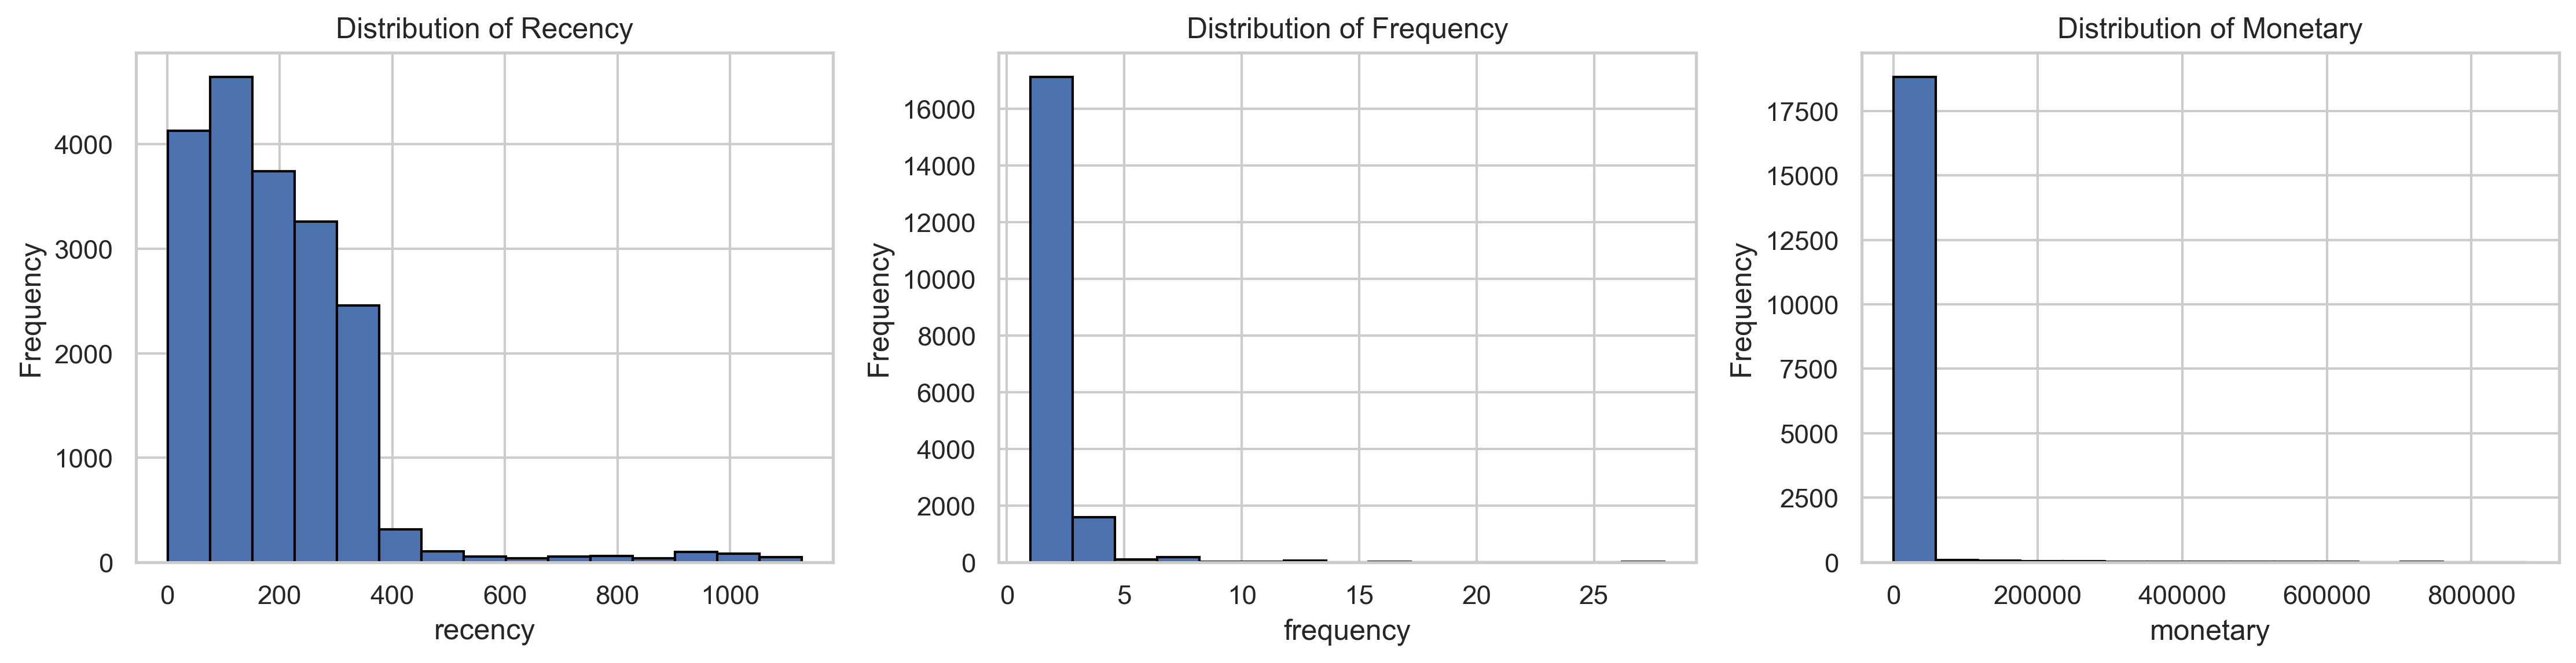
\includegraphics[keepaspectratio]{2-retail-analytics/../notebooks-and-scripts/2-retail-analytics/2-customer-value-and-retention/python/1-customer-value-and-retention-rfm-figures/rfm-feature-distributions.png}}

}

\caption{\label{fig-rfm-distributions}Distribution of the original RFM
variables before transformation.}

\end{figure}%

Several candidate values of (k) were evaluated using complementary
clustering diagnostics. Rather than relying on a single criterion, the
final solution balances cluster separation, compactness, and
interpretability. As summarised in Table~\ref{tbl-cluster-selection},
the nine-cluster solution provides the best overall compromise across
the internal validation metrics without producing unnecessarily
fragmented customer groups.

\begin{longtable}[]{@{}cccc@{}}
\caption{Clustering quality metrics used to determine the optimal number
of customer segments.}\label{tbl-cluster-selection}\tabularnewline
\toprule\noalign{}
k & Silhouette & Calinski--Harabasz & Davies--Bouldin \\
\midrule\noalign{}
\endfirsthead
\toprule\noalign{}
k & Silhouette & Calinski--Harabasz & Davies--Bouldin \\
\midrule\noalign{}
\endhead
\bottomrule\noalign{}
\endlastfoot
2 & 0.4435 & 15024.18 & 0.9683 \\
3 & 0.3890 & 13311.31 & 1.0315 \\
4 & 0.4035 & 12695.18 & 0.8897 \\
5 & 0.4237 & 13171.97 & 0.9205 \\
6 & 0.4267 & 13676.56 & 0.8533 \\
7 & 0.4348 & 14390.70 & 0.7965 \\
8 & 0.4556 & 15406.58 & 0.7315 \\
\textbf{9} & \textbf{0.4655} & \textbf{16264.65} & \textbf{0.7046} \\
10 & 0.4622 & 16513.19 & 0.7133 \\
\end{longtable}

The corresponding diagnostic curves are presented in
Figure~\ref{fig-cluster-selection}.

\begin{figure}

\centering{

\pandocbounded{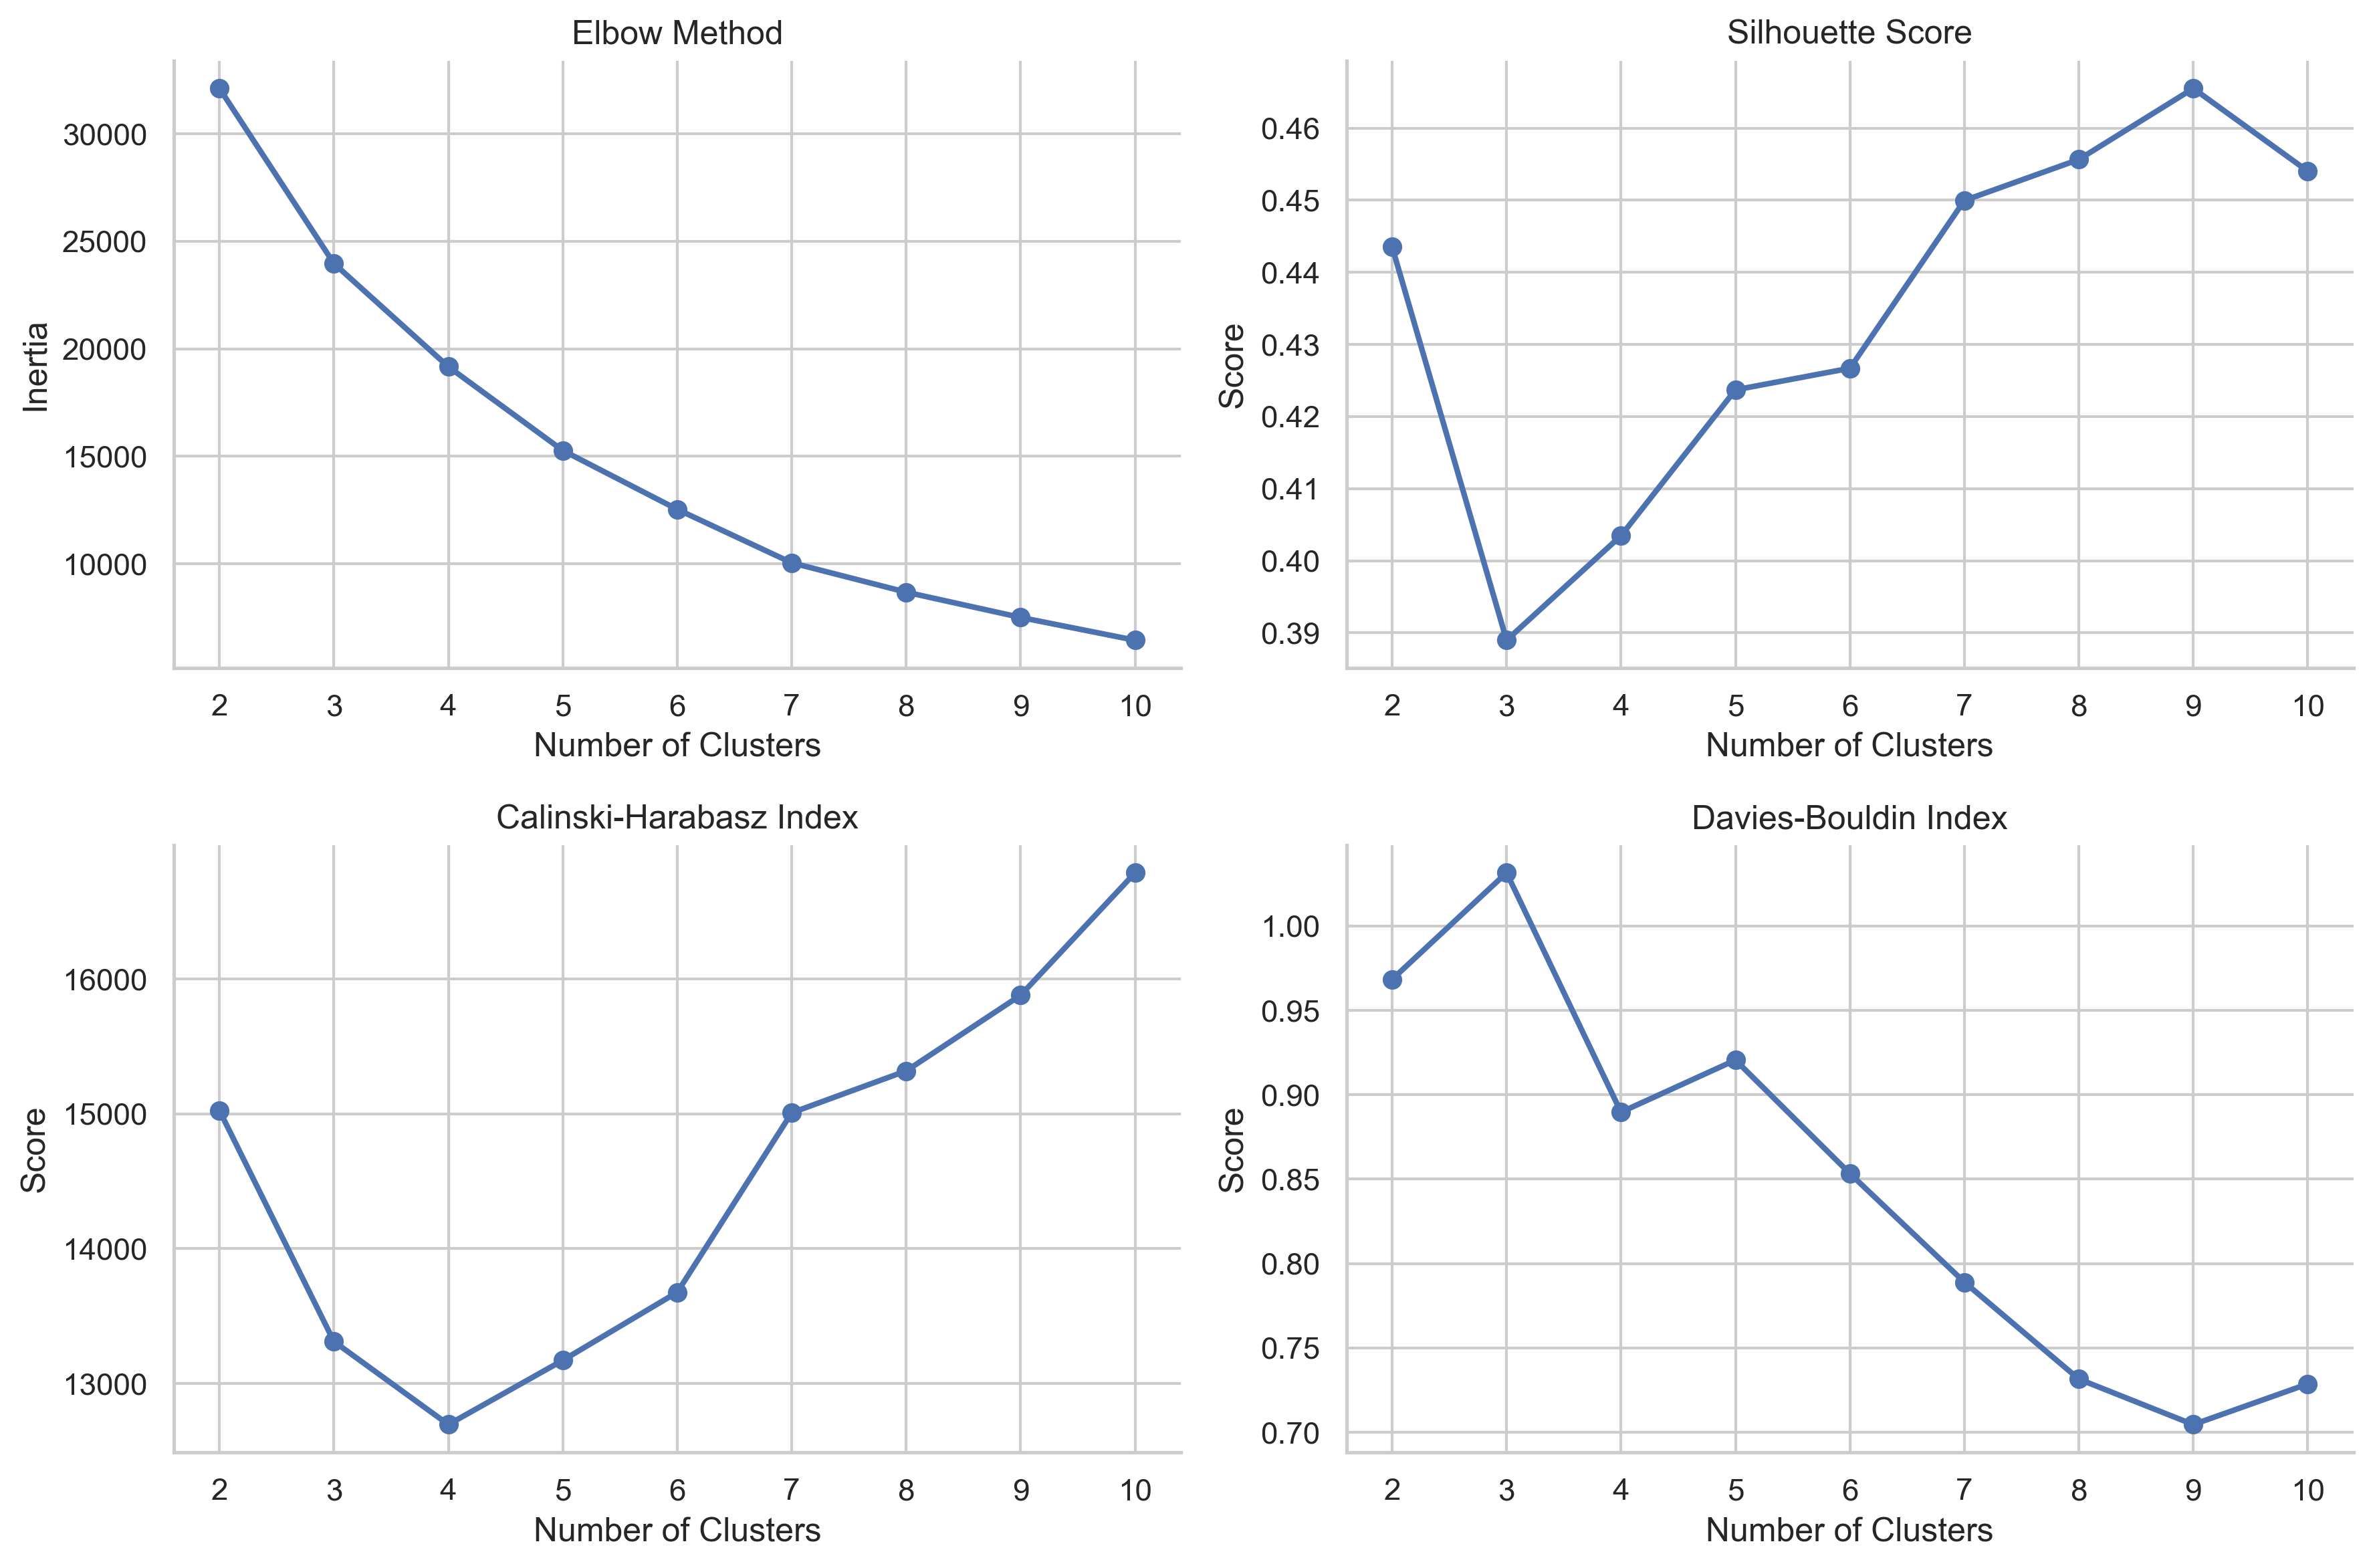
\includegraphics[keepaspectratio]{2-retail-analytics/../notebooks-and-scripts/2-retail-analytics/2-customer-value-and-retention/python/1-customer-value-and-retention-rfm-figures/cluster-selection-metrics.png}}

}

\caption{\label{fig-cluster-selection}Cluster selection diagnostics for
different values of (k).}

\end{figure}%

The selected segmentation identifies nine customer profiles that capture
meaningful differences in purchasing behaviour. Rather than representing
fixed customer categories, these segments describe behavioural
tendencies ranging from highly engaged customers to inactive, low-value
buyers. A summary of the resulting segments is presented in
Table~\ref{tbl-segment-summary}.

\begin{longtable}[]{@{}
  >{\centering\arraybackslash}p{(\linewidth - 10\tabcolsep) * \real{0.3494}}
  >{\centering\arraybackslash}p{(\linewidth - 10\tabcolsep) * \real{0.1205}}
  >{\centering\arraybackslash}p{(\linewidth - 10\tabcolsep) * \real{0.1084}}
  >{\centering\arraybackslash}p{(\linewidth - 10\tabcolsep) * \real{0.1446}}
  >{\centering\arraybackslash}p{(\linewidth - 10\tabcolsep) * \real{0.1205}}
  >{\centering\arraybackslash}p{(\linewidth - 10\tabcolsep) * \real{0.1566}}@{}}
\caption{Summary of the final customer segments obtained from the RFM
analysis.}\label{tbl-segment-summary}\tabularnewline
\toprule\noalign{}
\begin{minipage}[b]{\linewidth}\centering
Segment
\end{minipage} & \begin{minipage}[b]{\linewidth}\centering
Customers
\end{minipage} & \begin{minipage}[b]{\linewidth}\centering
Recency
\end{minipage} & \begin{minipage}[b]{\linewidth}\centering
Frequency
\end{minipage} & \begin{minipage}[b]{\linewidth}\centering
Monetary
\end{minipage} & \begin{minipage}[b]{\linewidth}\centering
Avg. Score
\end{minipage} \\
\midrule\noalign{}
\endfirsthead
\toprule\noalign{}
\begin{minipage}[b]{\linewidth}\centering
Segment
\end{minipage} & \begin{minipage}[b]{\linewidth}\centering
Customers
\end{minipage} & \begin{minipage}[b]{\linewidth}\centering
Recency
\end{minipage} & \begin{minipage}[b]{\linewidth}\centering
Frequency
\end{minipage} & \begin{minipage}[b]{\linewidth}\centering
Monetary
\end{minipage} & \begin{minipage}[b]{\linewidth}\centering
Avg. Score
\end{minipage} \\
\midrule\noalign{}
\endhead
\bottomrule\noalign{}
\endlastfoot
Champions & 2767 & 87.1 & 3.05 & 28042.2 & 0.74 \\
High Value but Cooling & 2832 & 264.0 & 2.27 & 8903.2 & 0.51 \\
Frequent Low-Spend Customers & 791 & 67.5 & 2.77 & 776.8 & 0.76 \\
Recent Low-Value Customers & 1724 & 87.3 & 1.00 & 1397.6 & 0.66 \\
Active Minimal Buyers & 2463 & 147.6 & 1.20 & 2145.7 & 0.63 \\
Declining Frequent Buyers & 1075 & 107.1 & 2.35 & 122.3 & 0.57 \\
Inactive Minimal Buyers & 4987 & 328.4 & 1.00 & 1054.6 & 0.35 \\
Inactive Low-Value Customers & 2046 & 274.7 & 1.00 & 1352.8 & 0.40 \\
Lost Customers & 434 & 845.6 & 1.01 & 2852.1 & 0.18 \\
\end{longtable}

The three-dimensional representation shown in Figure~\ref{fig-rfm-space}
highlights the gradual transition between behavioural groups rather than
sharply separated customer categories. This reinforces an important
practical point: customer segmentation should be interpreted as a
descriptive representation of purchasing behaviour rather than a
definitive classification of customer types.

\begin{figure}

\centering{

\pandocbounded{
\includegraphics[keepaspectratio]{2-retail-analytics/../notebooks-and-scripts/2-retail-analytics/2-customer-value-and-retention/python/1-customer-value-and-retention-rfm-figures/customer-segments-rfm-space.png}}

}

\caption{\label{fig-rfm-space}Three-dimensional representation of the
customer segments in the original RFM space.}

\end{figure}%

\subsection{Churn Prediction}\label{churn-prediction}

Customer segmentation provides a descriptive representation of
purchasing behaviour, but it does not indicate whether customers are
likely to remain active. The second stage of the workflow therefore
introduces a predictive component by estimating the probability that
each customer will become inactive during the observation period.

Several supervised learning algorithms were evaluated using the
engineered customer-level features described in the previous section.
Their performance is summarised in
Table~\ref{tbl-churn-model-comparison}. Rather than relying on a single
evaluation metric, the comparison considers both discrimination and
ranking performance to identify the model that provides the most
reliable estimates of customer retention risk.

\begin{longtable}[]{@{}
  >{\raggedright\arraybackslash}p{(\linewidth - 16\tabcolsep) * \real{0.1045}}
  >{\centering\arraybackslash}p{(\linewidth - 16\tabcolsep) * \real{0.1493}}
  >{\centering\arraybackslash}p{(\linewidth - 16\tabcolsep) * \real{0.1045}}
  >{\centering\arraybackslash}p{(\linewidth - 16\tabcolsep) * \real{0.1045}}
  >{\centering\arraybackslash}p{(\linewidth - 16\tabcolsep) * \real{0.1194}}
  >{\centering\arraybackslash}p{(\linewidth - 16\tabcolsep) * \real{0.1045}}
  >{\centering\arraybackslash}p{(\linewidth - 16\tabcolsep) * \real{0.1045}}
  >{\centering\arraybackslash}p{(\linewidth - 16\tabcolsep) * \real{0.1045}}
  >{\centering\arraybackslash}p{(\linewidth - 16\tabcolsep) * \real{0.1045}}@{}}
\caption{Performance comparison of the evaluated churn prediction
models. Abbreviations: RF = Random Forest; XGB = XGBoost; LR = Logistic
Regression; AP = Average Precision; BA = Balanced
Accuracy.}\label{tbl-churn-model-comparison}\tabularnewline
\toprule\noalign{}
\begin{minipage}[b]{\linewidth}\raggedright
Model
\end{minipage} & \begin{minipage}[b]{\linewidth}\centering
Sampling
\end{minipage} & \begin{minipage}[b]{\linewidth}\centering
AUC
\end{minipage} & \begin{minipage}[b]{\linewidth}\centering
AP
\end{minipage} & \begin{minipage}[b]{\linewidth}\centering
Acc.
\end{minipage} & \begin{minipage}[b]{\linewidth}\centering
BA
\end{minipage} & \begin{minipage}[b]{\linewidth}\centering
Prec.
\end{minipage} & \begin{minipage}[b]{\linewidth}\centering
Rec.
\end{minipage} & \begin{minipage}[b]{\linewidth}\centering
F1
\end{minipage} \\
\midrule\noalign{}
\endfirsthead
\toprule\noalign{}
\begin{minipage}[b]{\linewidth}\raggedright
Model
\end{minipage} & \begin{minipage}[b]{\linewidth}\centering
Sampling
\end{minipage} & \begin{minipage}[b]{\linewidth}\centering
AUC
\end{minipage} & \begin{minipage}[b]{\linewidth}\centering
AP
\end{minipage} & \begin{minipage}[b]{\linewidth}\centering
Acc.
\end{minipage} & \begin{minipage}[b]{\linewidth}\centering
BA
\end{minipage} & \begin{minipage}[b]{\linewidth}\centering
Prec.
\end{minipage} & \begin{minipage}[b]{\linewidth}\centering
Rec.
\end{minipage} & \begin{minipage}[b]{\linewidth}\centering
F1
\end{minipage} \\
\midrule\noalign{}
\endhead
\bottomrule\noalign{}
\endlastfoot
RF & SMOTE & 1.000 & 0.971 & 0.997 & 0.999 & 0.800 & 1.000 & 0.889 \\
XGB & Under & 1.000 & 0.951 & 0.987 & 0.994 & 0.455 & 1.000 & 0.625 \\
RF & Original & 1.000 & 0.959 & 0.997 & 0.949 & 0.857 & 0.900 & 0.878 \\
XGB & SMOTE & 0.999 & 0.960 & 0.997 & 0.949 & 0.857 & 0.900 & 0.878 \\
XGB & Original & 0.999 & 0.951 & 0.998 & 0.950 & 0.900 & 0.900 &
0.900 \\
RF & Under & 0.999 & 0.939 & 0.965 & 0.982 & 0.233 & 1.000 & 0.377 \\
LR & SMOTE & 0.999 & 0.892 & 0.987 & 0.994 & 0.455 & 1.000 & 0.625 \\
LR & Original & 0.998 & 0.871 & 0.996 & 0.849 & 0.875 & 0.700 & 0.778 \\
LR & Under & 0.997 & 0.829 & 0.969 & 0.984 & 0.256 & 1.000 & 0.408 \\
\end{longtable}

The best-performing specification was the Random Forest model trained
with SMOTE. As shown in Table~\ref{tbl-best-churn-model}, it achieved
excellent discrimination on the independent test set, with a ROC AUC of
0.9996 and an Average Precision of 0.9707. More importantly, the model
maintained full recall for the churn class while keeping precision at
0.8000, which is a useful balance for retention-oriented applications
where missing high-risk customers is usually more costly than reviewing
a small number of false positives.

\begin{longtable}[]{@{}
  >{\centering\arraybackslash}p{(\linewidth - 12\tabcolsep) * \real{0.1039}}
  >{\centering\arraybackslash}p{(\linewidth - 12\tabcolsep) * \real{0.2338}}
  >{\centering\arraybackslash}p{(\linewidth - 12\tabcolsep) * \real{0.1169}}
  >{\centering\arraybackslash}p{(\linewidth - 12\tabcolsep) * \real{0.2338}}
  >{\centering\arraybackslash}p{(\linewidth - 12\tabcolsep) * \real{0.1299}}
  >{\centering\arraybackslash}p{(\linewidth - 12\tabcolsep) * \real{0.0909}}
  >{\centering\arraybackslash}p{(\linewidth - 12\tabcolsep) * \real{0.0909}}@{}}
\caption{Performance of the selected churn prediction model on the
independent test set.}\label{tbl-best-churn-model}\tabularnewline
\toprule\noalign{}
\begin{minipage}[b]{\linewidth}\centering
ROC AUC
\end{minipage} & \begin{minipage}[b]{\linewidth}\centering
Average Precision
\end{minipage} & \begin{minipage}[b]{\linewidth}\centering
Accuracy
\end{minipage} & \begin{minipage}[b]{\linewidth}\centering
Balanced Accuracy
\end{minipage} & \begin{minipage}[b]{\linewidth}\centering
Precision
\end{minipage} & \begin{minipage}[b]{\linewidth}\centering
Recall
\end{minipage} & \begin{minipage}[b]{\linewidth}\centering
F1
\end{minipage} \\
\midrule\noalign{}
\endfirsthead
\toprule\noalign{}
\begin{minipage}[b]{\linewidth}\centering
ROC AUC
\end{minipage} & \begin{minipage}[b]{\linewidth}\centering
Average Precision
\end{minipage} & \begin{minipage}[b]{\linewidth}\centering
Accuracy
\end{minipage} & \begin{minipage}[b]{\linewidth}\centering
Balanced Accuracy
\end{minipage} & \begin{minipage}[b]{\linewidth}\centering
Precision
\end{minipage} & \begin{minipage}[b]{\linewidth}\centering
Recall
\end{minipage} & \begin{minipage}[b]{\linewidth}\centering
F1
\end{minipage} \\
\midrule\noalign{}
\endhead
\bottomrule\noalign{}
\endlastfoot
0.9996 & 0.9707 & 0.9973 & 0.9986 & 0.8000 & 1.0000 & 0.8889 \\
\end{longtable}

The class-level results in Table~\ref{tbl-classification-report} provide
a more detailed view of the same behaviour. The model correctly
identifies all churn cases in the test set, while most retention cases
are also classified correctly. This is particularly relevant because the
churn class is very small relative to the retained customer population.

\begin{longtable}[]{@{}ccccc@{}}
\caption{Precision, Recall, F1-score, and support for the selected churn
prediction model.}\label{tbl-classification-report}\tabularnewline
\toprule\noalign{}
Class & Precision & Recall & F1-score & Support \\
\midrule\noalign{}
\endfirsthead
\toprule\noalign{}
Class & Precision & Recall & F1-score & Support \\
\midrule\noalign{}
\endhead
\bottomrule\noalign{}
\endlastfoot
Retention & 1.0000 & 0.9973 & 0.9986 & 1842 \\
Churn & 0.8000 & 1.0000 & 0.8889 & 20 \\
Accuracy & 0.9973 & 0.9973 & 0.9973 & 0.9973 \\
Macro avg & 0.9000 & 0.9986 & 0.9438 & 1862 \\
Weighted avg & 0.9979 & 0.9973 & 0.9975 & 1862 \\
\end{longtable}

The Receiver Operating Characteristic curve presented in
Figure~\ref{fig-roc} demonstrates that the model separates active and
inactive customers across a broad range of decision thresholds. Since
customer retention datasets are inherently imbalanced, the
Precision--Recall curve shown in Figure~\ref{fig-pr-curve} provides an
equally important perspective by evaluating the model's ability to
identify genuinely high-risk customers without generating an excessive
number of false positives.

\begin{figure}

\centering{

\pandocbounded{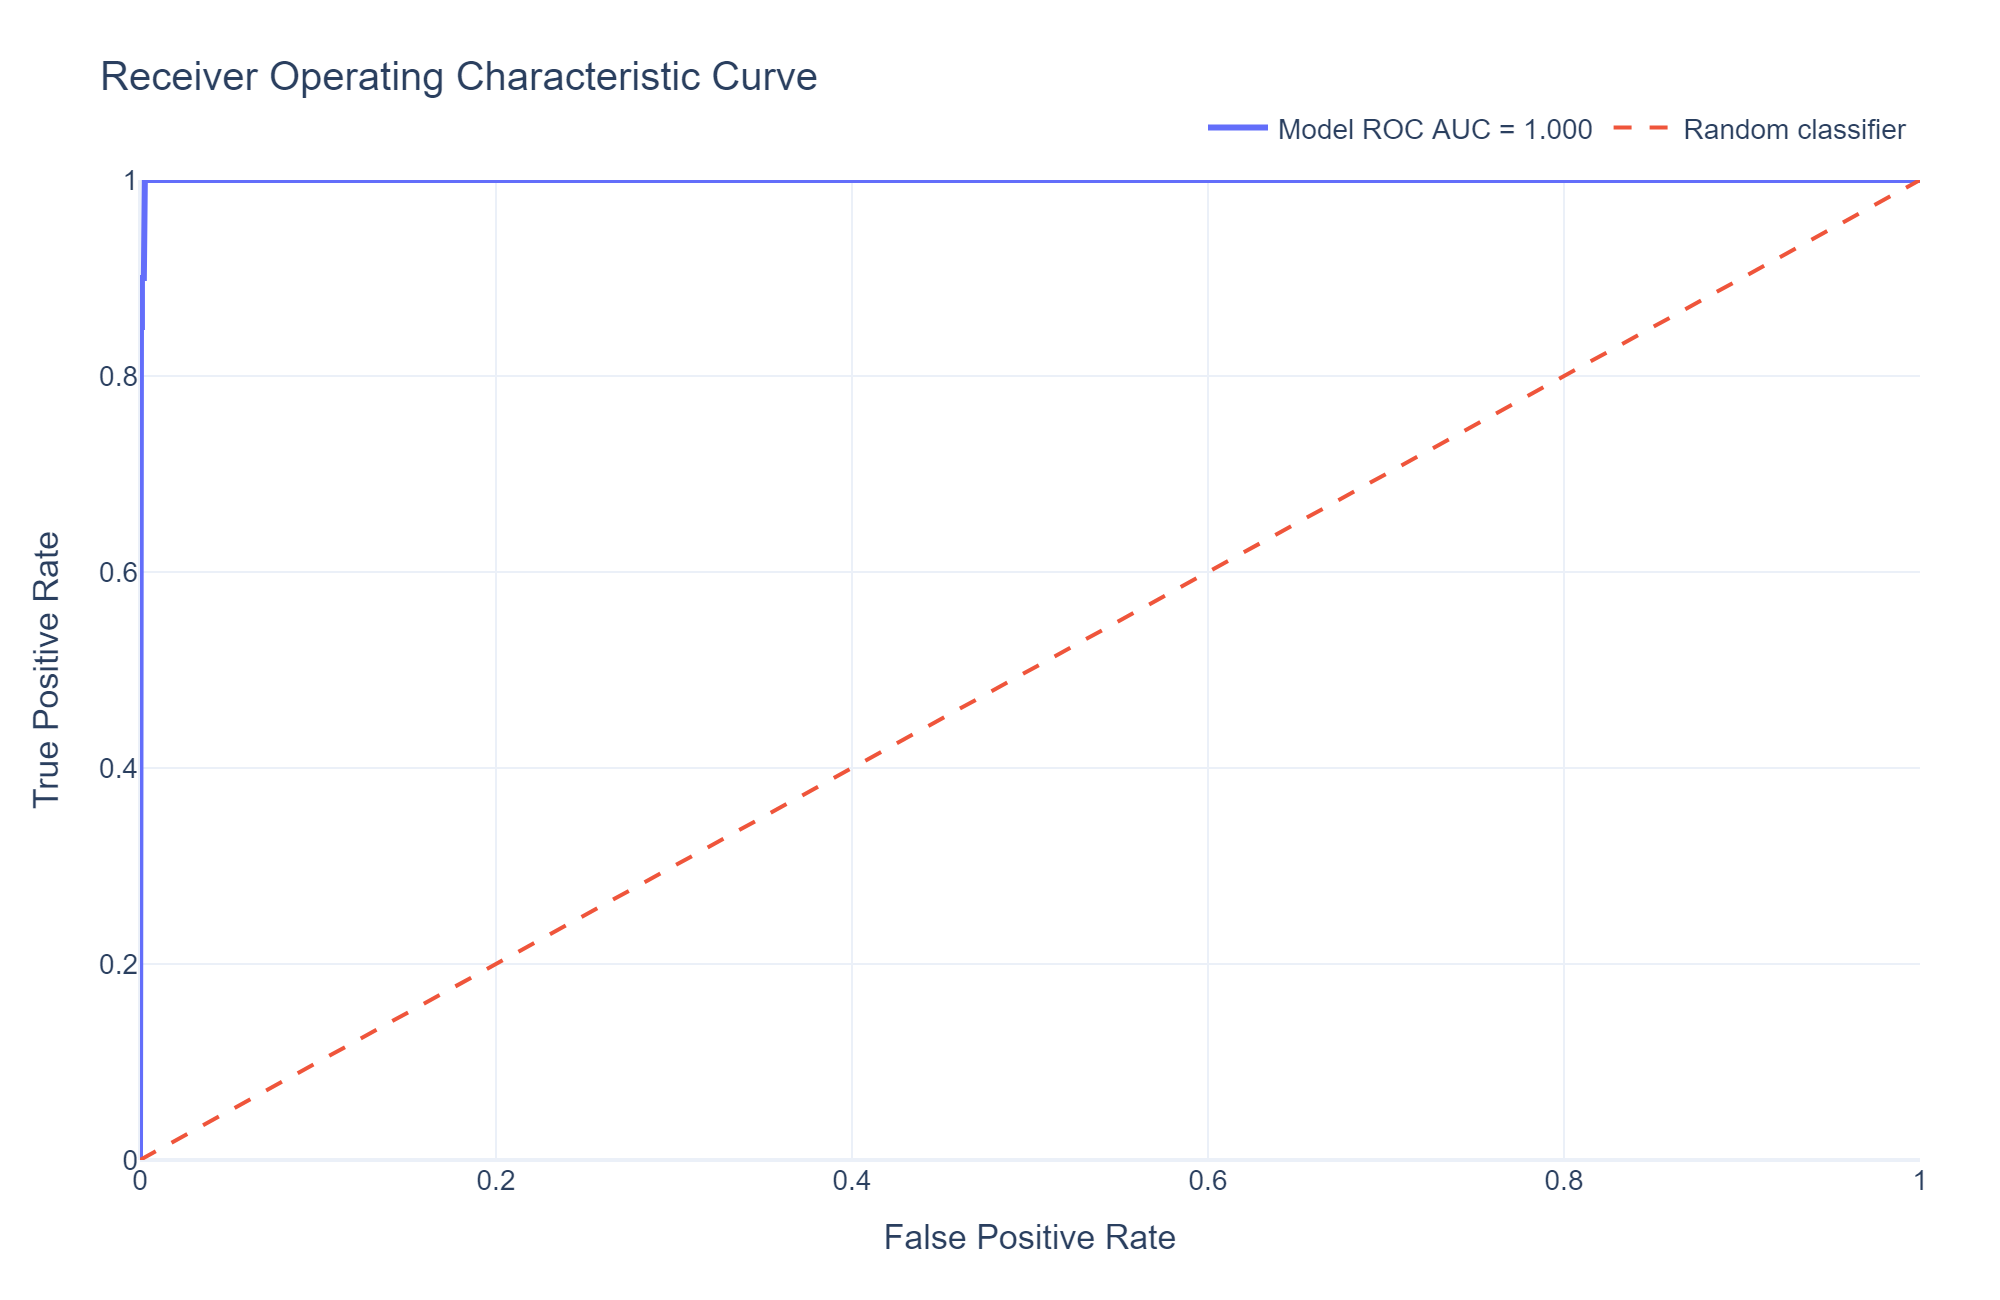
\includegraphics[keepaspectratio]{2-retail-analytics/../notebooks-and-scripts/2-retail-analytics/2-customer-value-and-retention/python/2-customer-value-and-retention-churn-figures/roc-curve.png}}

}

\caption{\label{fig-roc}Receiver Operating Characteristic curve for the
selected churn prediction model.}

\end{figure}%

\begin{figure}

\centering{

\pandocbounded{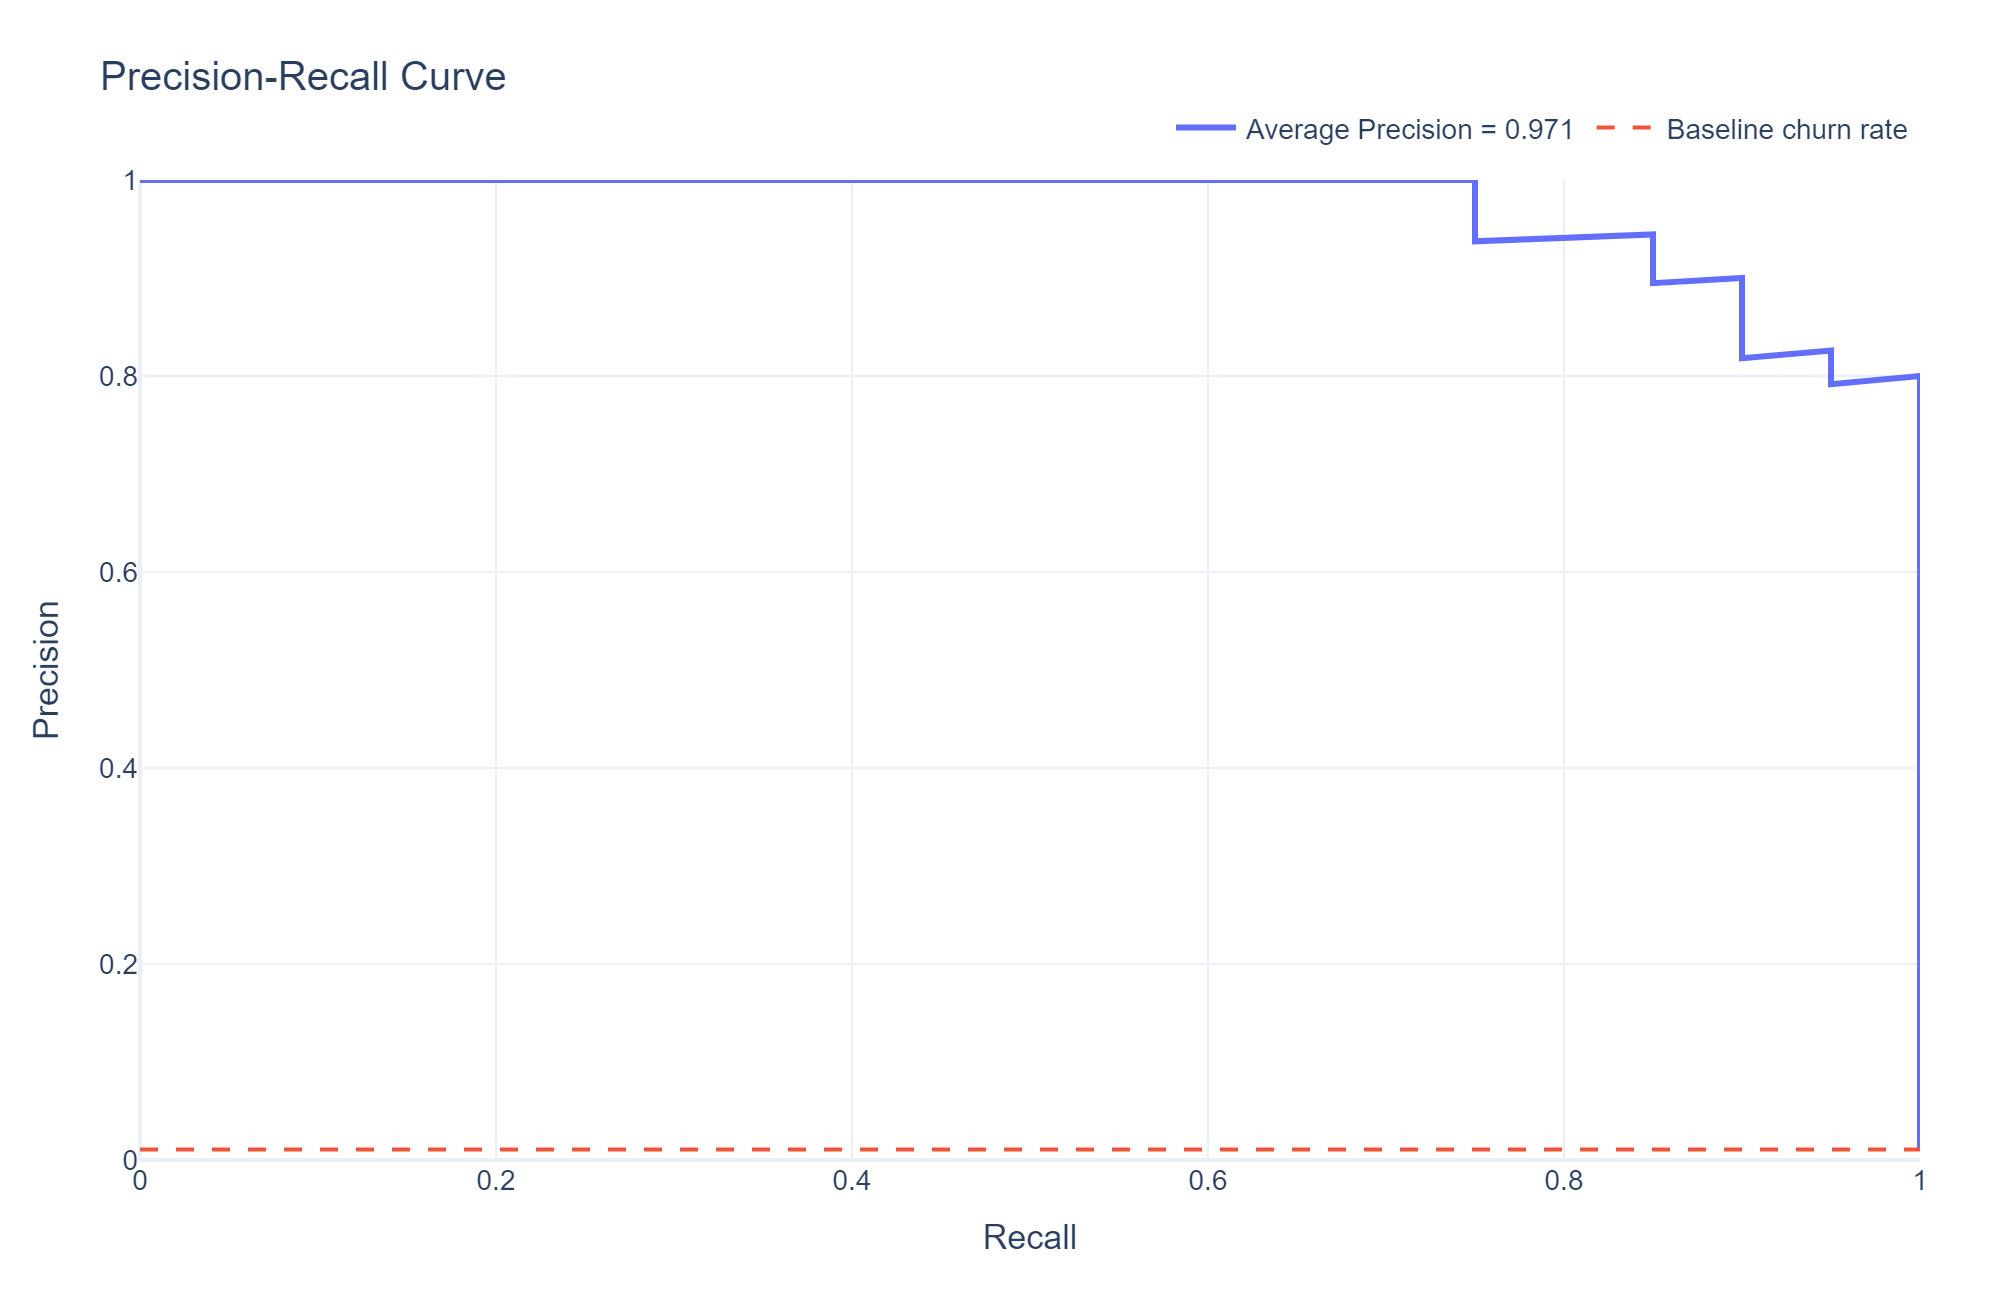
\includegraphics[keepaspectratio]{2-retail-analytics/../notebooks-and-scripts/2-retail-analytics/2-customer-value-and-retention/python/2-customer-value-and-retention-churn-figures/precision-recall-curve.png}}

}

\caption{\label{fig-pr-curve}Precision--Recall curve for the selected
churn prediction model.}

\end{figure}%

The confusion matrix shown in Figure~\ref{fig-confusion-matrix}
reinforces this interpretation. Most customers are correctly classified,
while the remaining errors reflect the intrinsic uncertainty associated
with non-contractual customer behaviour. In this setting, some customers
naturally purchase at irregular intervals, making it difficult to
distinguish perfectly between temporary inactivity and progressive
disengagement.

\begin{figure}

\centering{

\pandocbounded{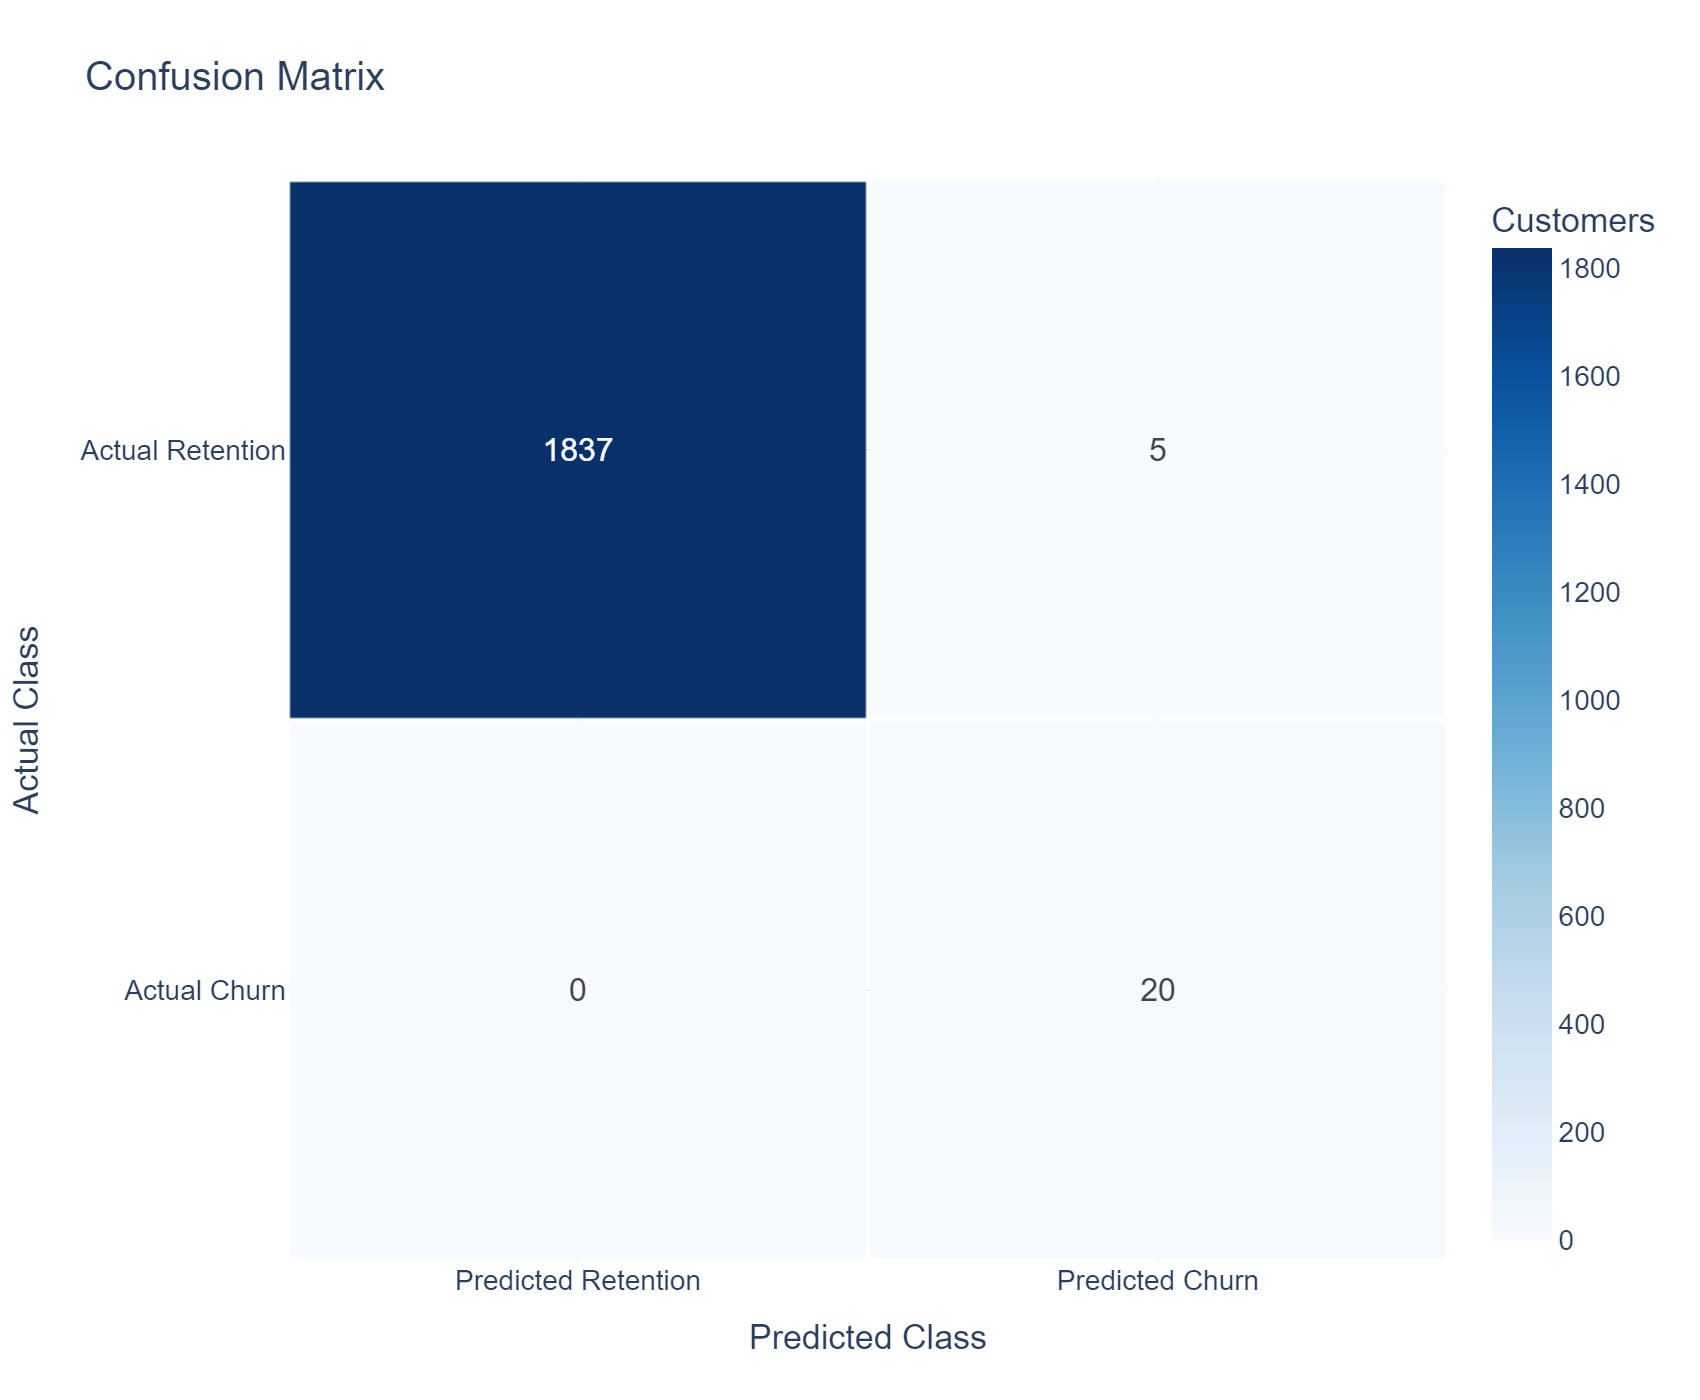
\includegraphics[keepaspectratio]{2-retail-analytics/../notebooks-and-scripts/2-retail-analytics/2-customer-value-and-retention/python/2-customer-value-and-retention-churn-figures/confusion-matrix.png}}

}

\caption{\label{fig-confusion-matrix}Confusion matrix for the selected
churn prediction model.}

\end{figure}%

From a business perspective, ranking customers by estimated churn
probability is often more useful than producing binary predictions.
Marketing teams typically have limited resources and cannot intervene
with every customer simultaneously. The cumulative gains curve shown in
Figure~\ref{fig-cumulative-gains} demonstrates that the model
concentrates a substantial proportion of future churners within the
highest-risk customers, enabling retention campaigns to be prioritised
more effectively.

\begin{figure}

\centering{

\pandocbounded{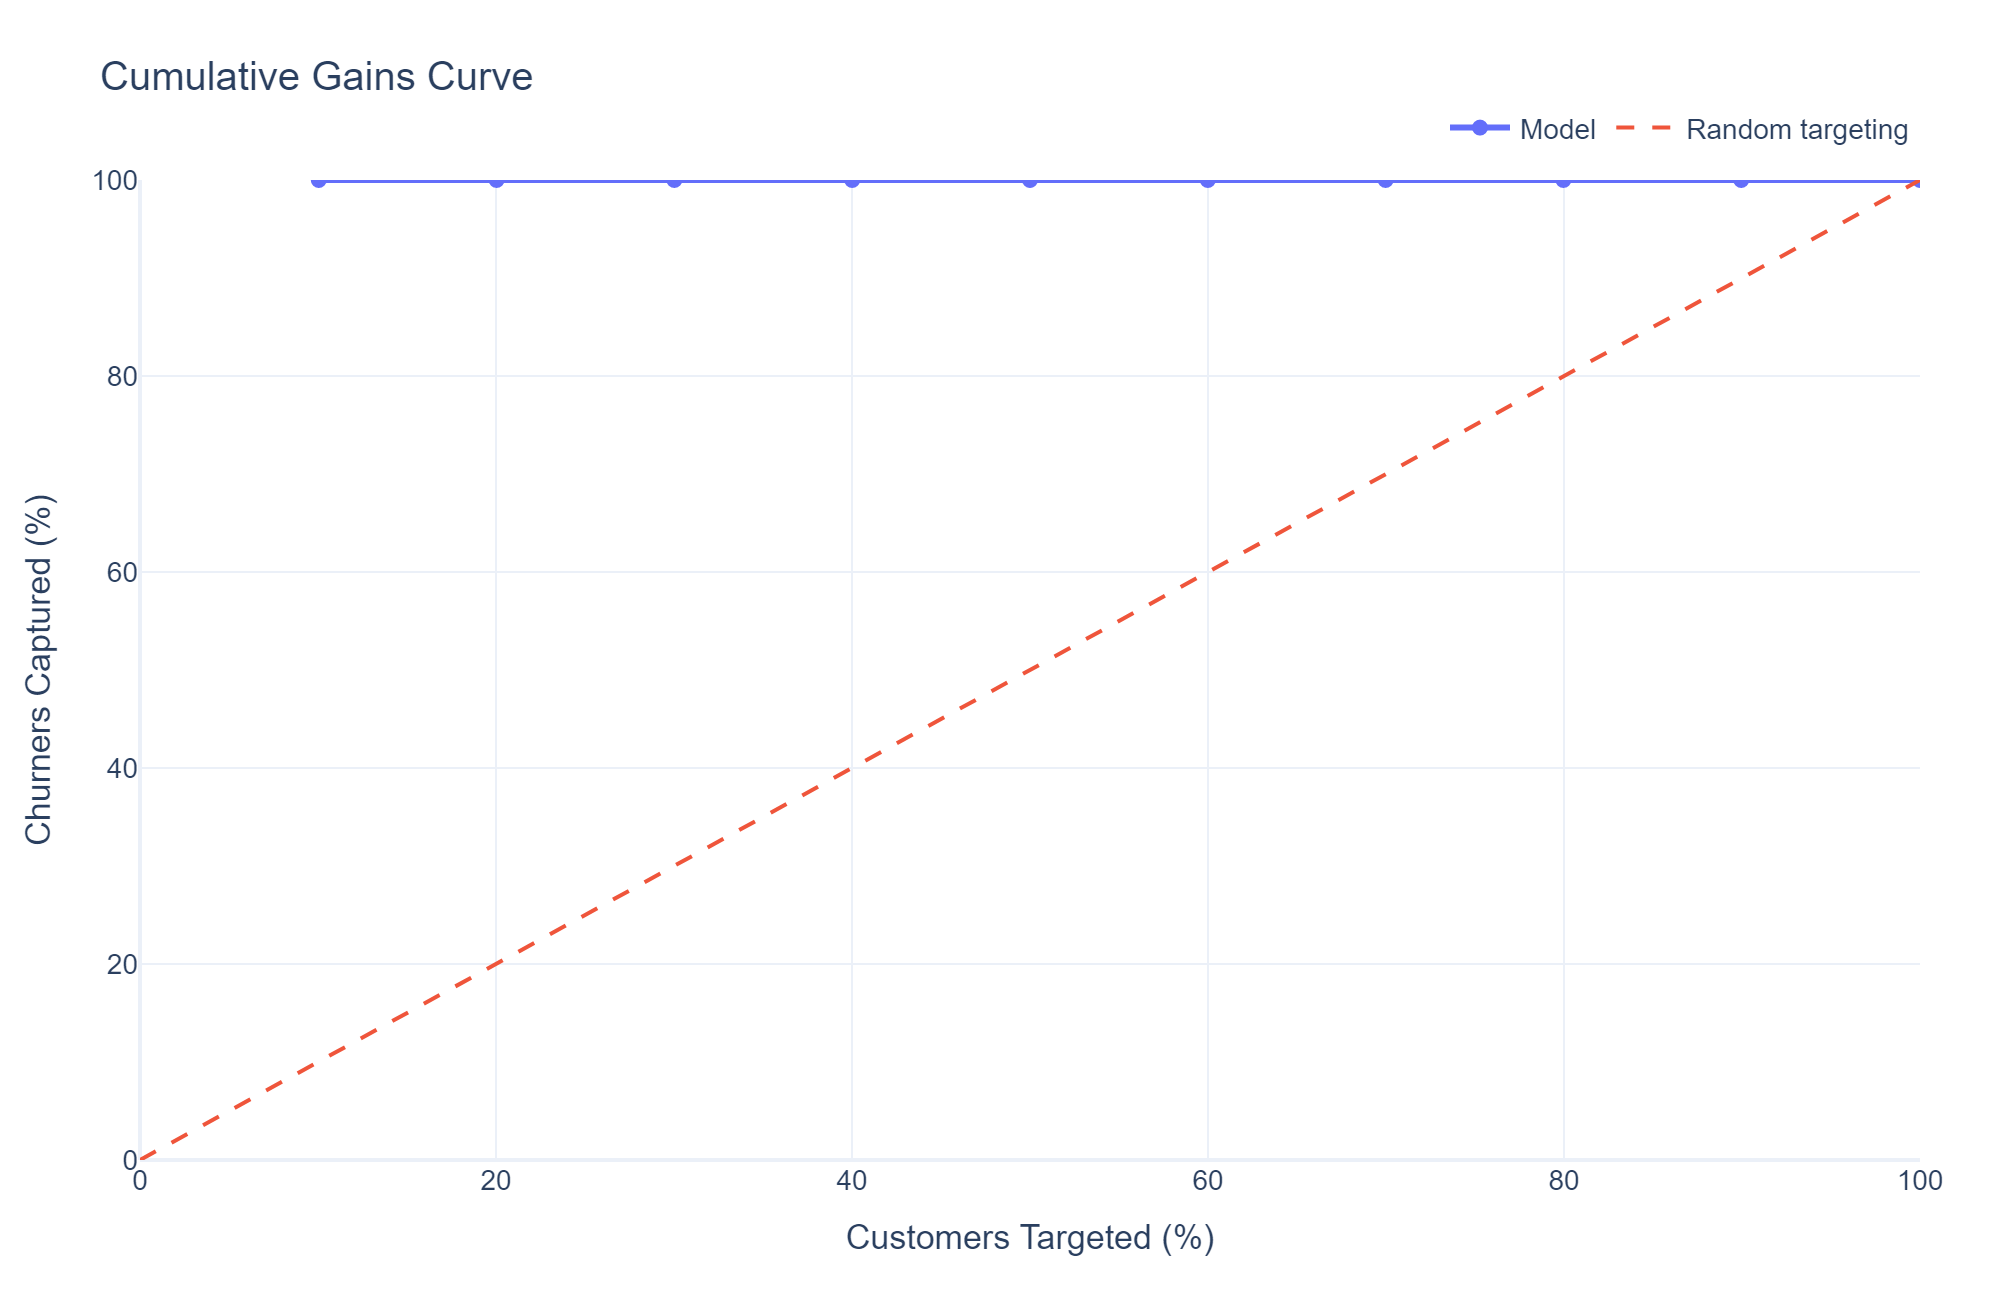
\includegraphics[keepaspectratio]{2-retail-analytics/../notebooks-and-scripts/2-retail-analytics/2-customer-value-and-retention/python/2-customer-value-and-retention-churn-figures/cumulative-gains-curve.png}}

}

\caption{\label{fig-cumulative-gains}Cumulative gains curve for the
selected churn prediction model.}

\end{figure}%

Inspection of the feature importance rankings further supports the
behavioural interpretation of the model. As shown in
Figure~\ref{fig-feature-importance}, variables related to purchasing
recency, customer tenure, purchasing cadence, and behavioural
segmentation contribute substantially to the predicted probabilities.
This consistency suggests that the model is learning meaningful patterns
associated with customer engagement rather than relying on spurious
statistical relationships.

\begin{figure}

\centering{

\pandocbounded{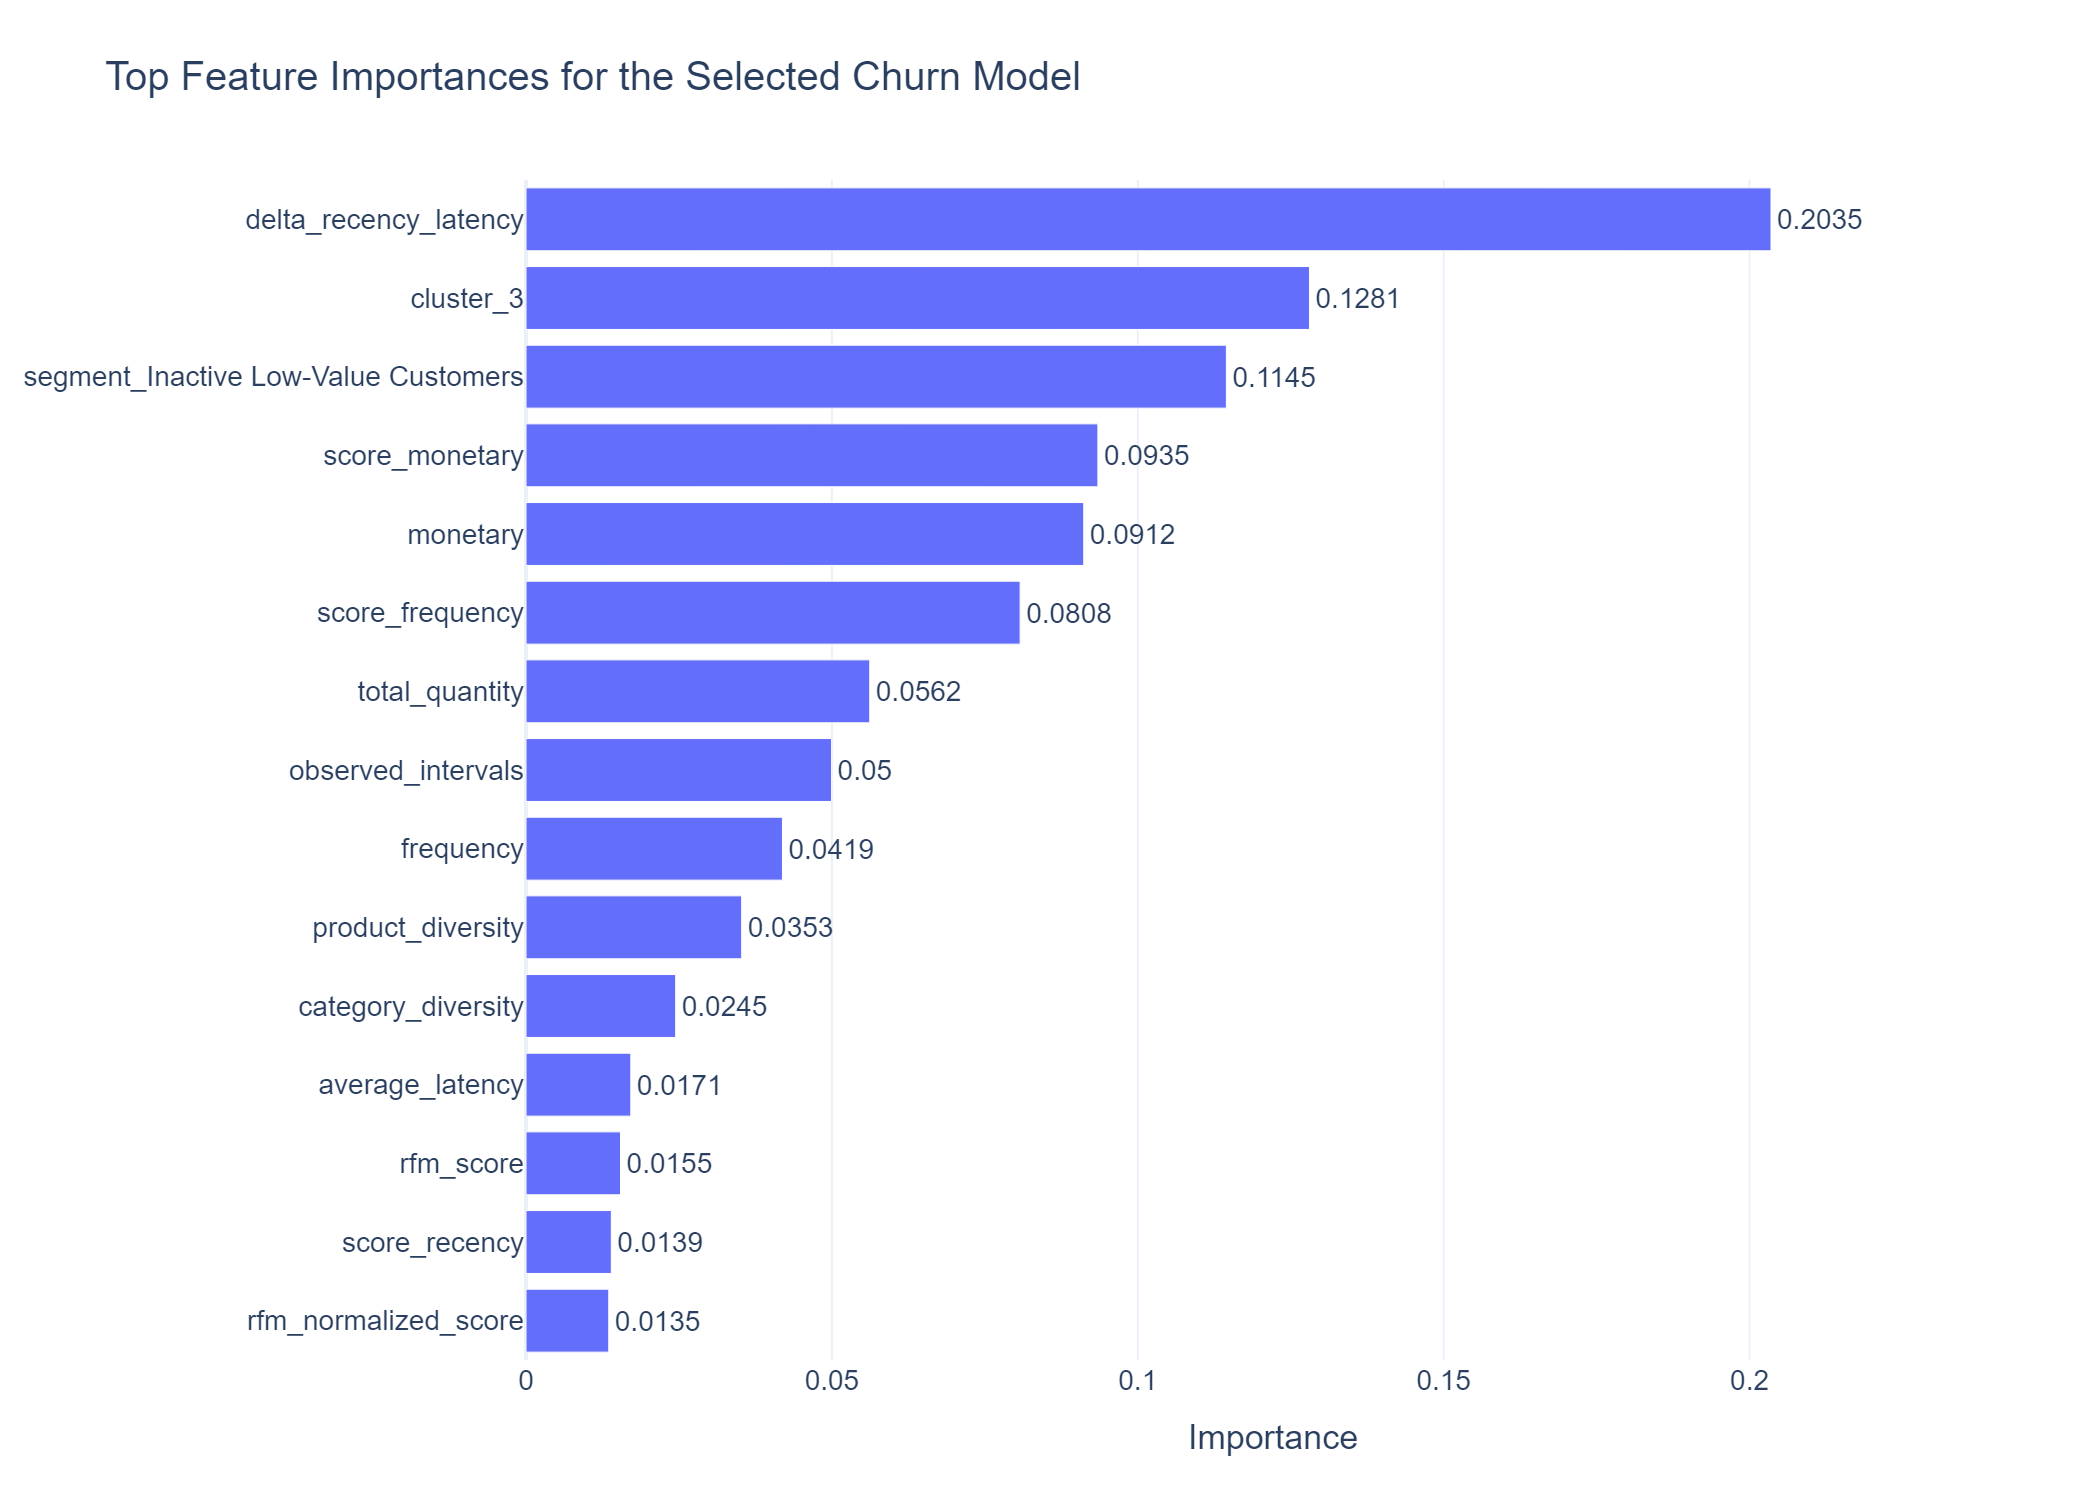
\includegraphics[keepaspectratio]{2-retail-analytics/../notebooks-and-scripts/2-retail-analytics/2-customer-value-and-retention/python/2-customer-value-and-retention-churn-figures/top-feature-importances.png}}

}

\caption{\label{fig-feature-importance}Feature importance for the
selected churn prediction model.}

\end{figure}%

Although the predictive performance is strong, several limitations
should be acknowledged. The model depends on the operational definition
of churn adopted in this project, meaning that alternative calibration
or observation windows would naturally produce different labels. The
churn class is also small in absolute terms, so the excellent
performance metrics should be interpreted with caution. The predicted
probabilities quantify behavioural risk rather than certainty, and
customers identified as high risk should be understood as candidates for
proactive retention strategies rather than customers who have
definitively left the business.

\subsection{Risk-Adjusted Customer Lifetime Value
Prediction}\label{risk-adjusted-customer-lifetime-value-prediction-1}

The final stage of the workflow integrates customer profitability with
the behavioural information obtained during the segmentation and churn
analyses. Rather than estimating customer value exclusively from
historical purchases, the objective is to approximate a risk-adjusted
valuation that combines observed profitability with expected customer
retention. This produces a more realistic prioritisation framework by
recognising that customers with similar historical revenue may
contribute very differently to future business performance.

Several regression algorithms were evaluated using the customer-level
features engineered throughout the project. Their predictive performance
is summarised in Table~\ref{tbl-clv-model-comparison}. The Random Forest
regressor achieved the best overall performance, with the lowest RMSE
and MAE and the highest (R\^{}2), indicating that it reproduced the
constructed valuation framework more accurately than the other candidate
models.

\begin{longtable}[]{@{}
  >{\centering\arraybackslash}p{(\linewidth - 6\tabcolsep) * \real{0.5082}}
  >{\centering\arraybackslash}p{(\linewidth - 6\tabcolsep) * \real{0.1803}}
  >{\centering\arraybackslash}p{(\linewidth - 6\tabcolsep) * \real{0.1803}}
  >{\centering\arraybackslash}p{(\linewidth - 6\tabcolsep) * \real{0.1311}}@{}}
\caption{Performance comparison of the evaluated Customer Lifetime Value
prediction models.}\label{tbl-clv-model-comparison}\tabularnewline
\toprule\noalign{}
\begin{minipage}[b]{\linewidth}\centering
Model
\end{minipage} & \begin{minipage}[b]{\linewidth}\centering
RMSE
\end{minipage} & \begin{minipage}[b]{\linewidth}\centering
MAE
\end{minipage} & \begin{minipage}[b]{\linewidth}\centering
\(R^2\)
\end{minipage} \\
\midrule\noalign{}
\endfirsthead
\toprule\noalign{}
\begin{minipage}[b]{\linewidth}\centering
Model
\end{minipage} & \begin{minipage}[b]{\linewidth}\centering
RMSE
\end{minipage} & \begin{minipage}[b]{\linewidth}\centering
MAE
\end{minipage} & \begin{minipage}[b]{\linewidth}\centering
\(R^2\)
\end{minipage} \\
\midrule\noalign{}
\endhead
\bottomrule\noalign{}
\endlastfoot
Random Forest & 1936.5286 & 345.9793 & 0.9966 \\
XGBoost & 2178.4778 & 473.2691 & 0.9957 \\
Regression Tree & 2607.8713 & 456.9903 & 0.9938 \\
K-Nearest Neighbors Regression & 4066.1658 & 880.0326 & 0.9850 \\
Ridge Regression & 8251.9469 & 4268.8566 & 0.9384 \\
LASSO Regression & 8300.8116 & 4313.9835 & 0.9377 \\
Linear Regression & 8316.9955 & 4332.1693 & 0.9374 \\
Support Vector Regression & 35181.7991 & 19710.3313 & -0.1193 \\
\end{longtable}

The selected model was then evaluated on the independent test set. As
reported in Table~\ref{tbl-final-clv-model}, the final Random Forest
model retained very strong predictive performance, explaining most of
the variation in the constructed CLV target while keeping the average
absolute error relatively small.

\begin{longtable}[]{@{}cccc@{}}
\caption{Predictive performance of the selected Customer Lifetime Value
model on the independent test
set.}\label{tbl-final-clv-model}\tabularnewline
\toprule\noalign{}
Model & RMSE & MAE & \(R^2\) \\
\midrule\noalign{}
\endfirsthead
\toprule\noalign{}
Model & RMSE & MAE & \(R^2\) \\
\midrule\noalign{}
\endhead
\bottomrule\noalign{}
\endlastfoot
Random Forest & 2028.6151 & 363.8659 & 0.9963 \\
\end{longtable}

The relationship between predicted and observed customer lifetime values
is illustrated in Figure~\ref{fig-predicted-vs-actual}. Most
observations are concentrated around the identity line, indicating that
the regression model successfully reproduces the underlying valuation
framework across a broad range of customer values. The residual analysis
shown in Figure~\ref{fig-residuals} further suggests that no major
systematic prediction bias is present, although variability naturally
increases for the highest-value customers, which represent only a small
fraction of the customer base.

\begin{figure}

\centering{

\pandocbounded{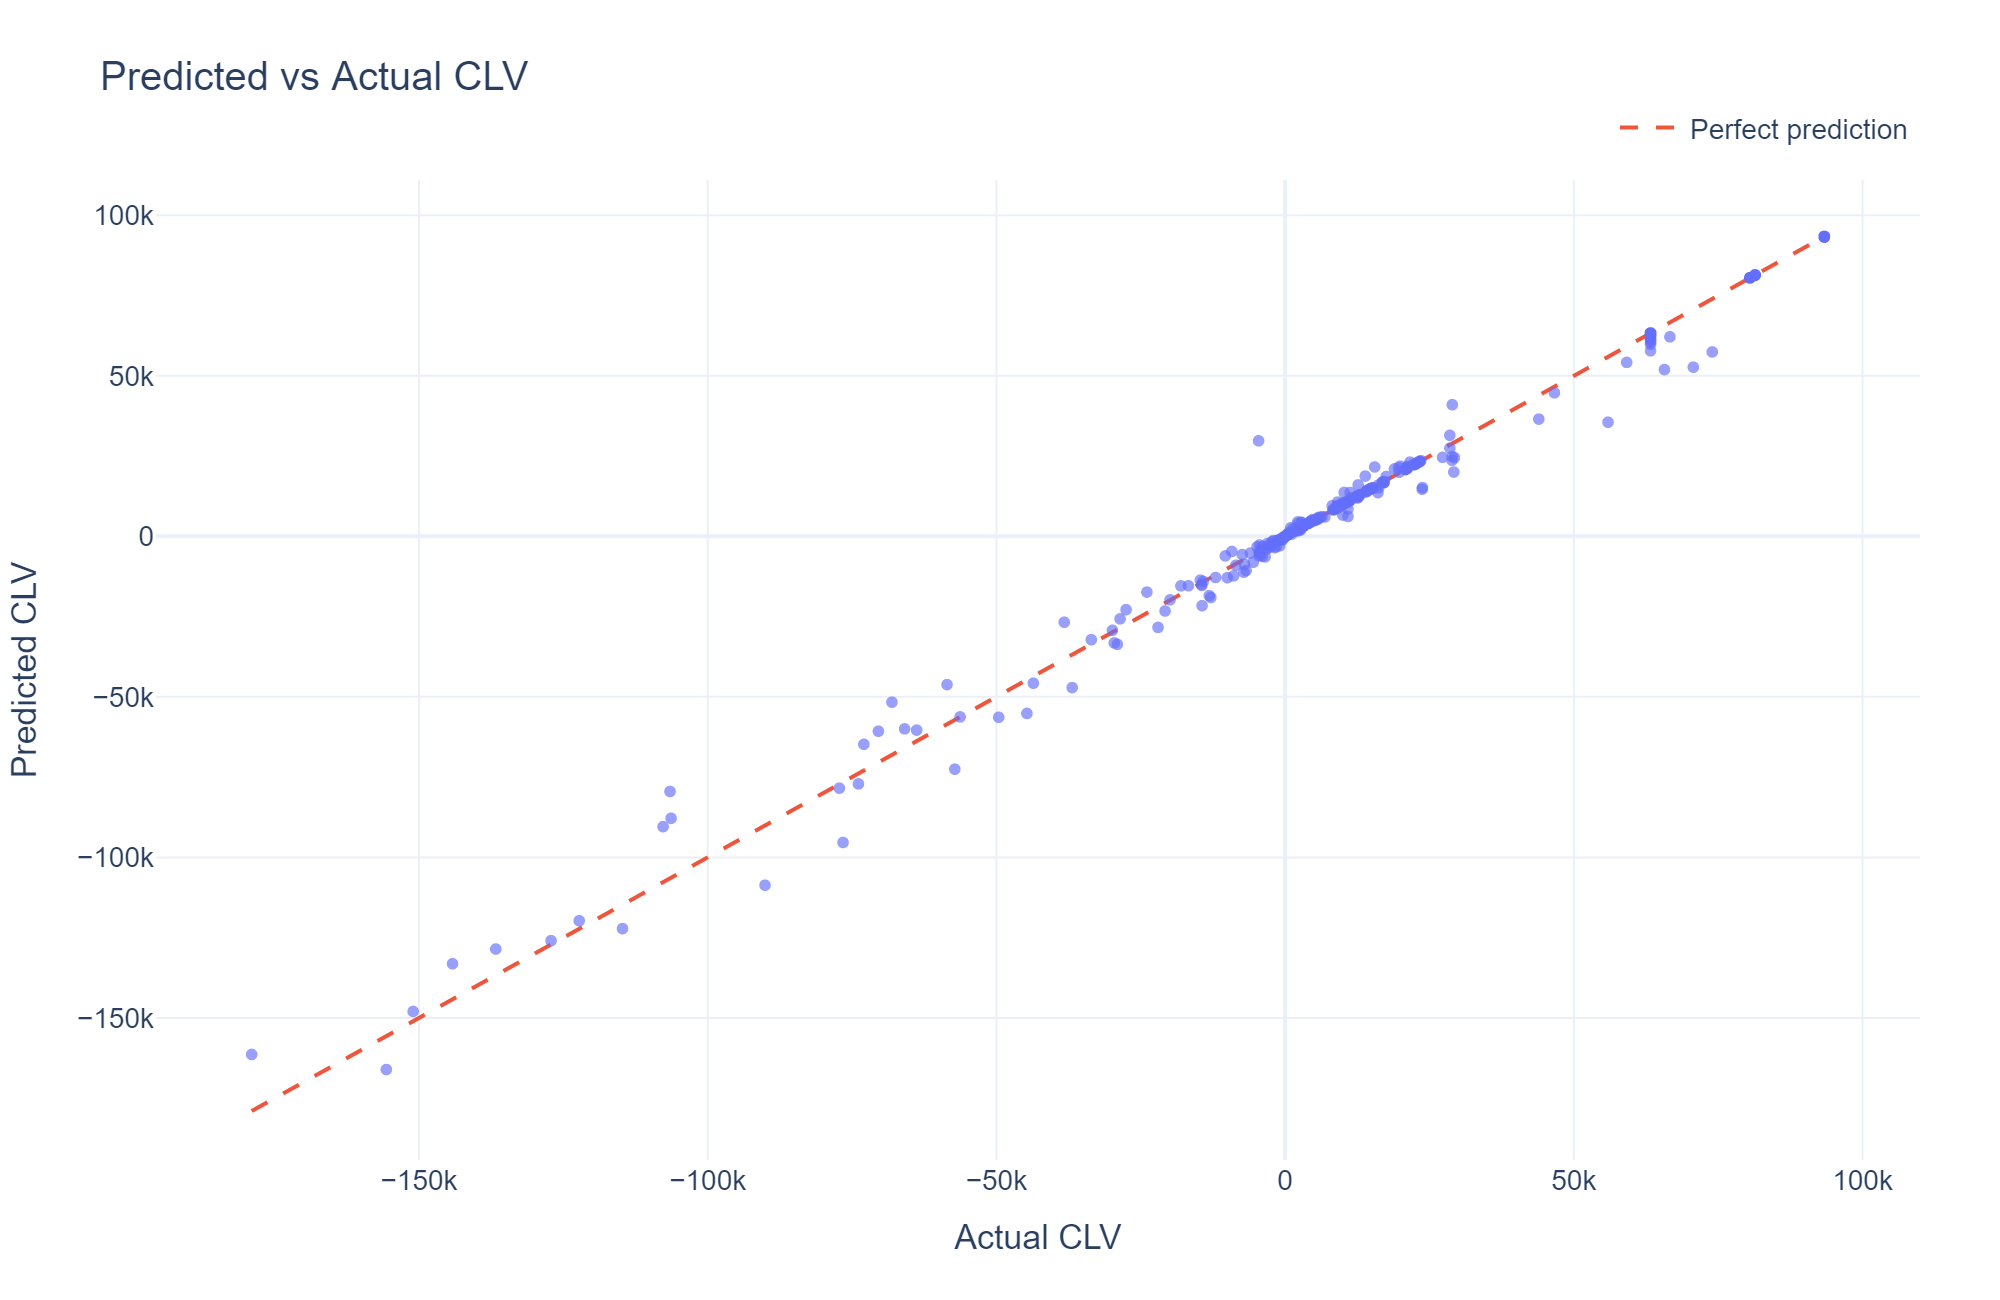
\includegraphics[keepaspectratio]{2-retail-analytics/../notebooks-and-scripts/2-retail-analytics/2-customer-value-and-retention/python/3-customer-value-and-retention-clv-figures/predicted-vs-actual-clv.png}}

}

\caption{\label{fig-predicted-vs-actual}Predicted versus observed
Customer Lifetime Value on the independent test set.}

\end{figure}%

\begin{figure}

\centering{

\pandocbounded{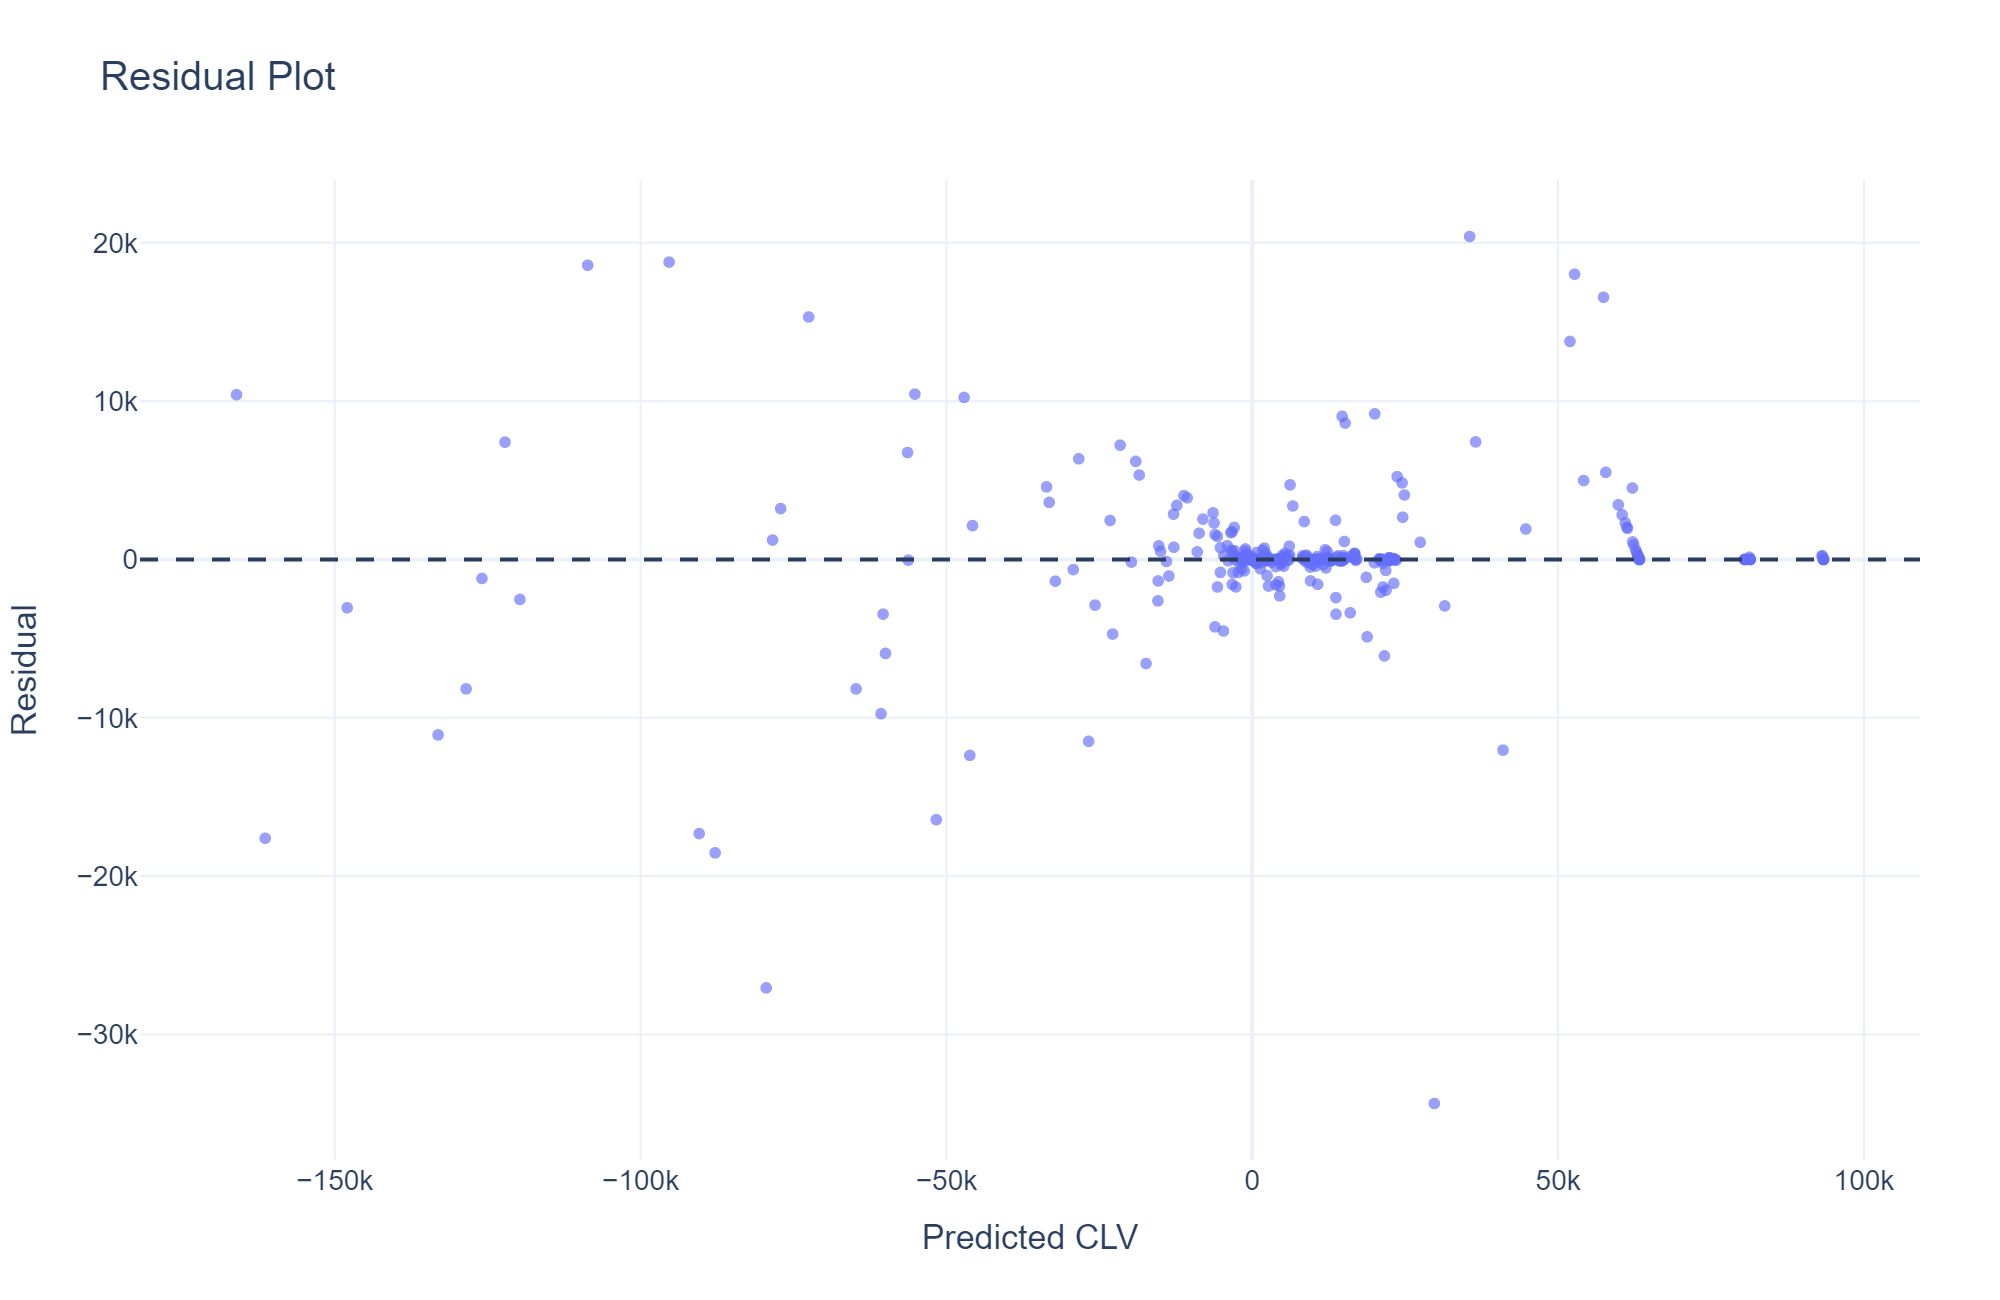
\includegraphics[keepaspectratio]{2-retail-analytics/../notebooks-and-scripts/2-retail-analytics/2-customer-value-and-retention/python/3-customer-value-and-retention-clv-figures/residual-plot.png}}

}

\caption{\label{fig-residuals}Residual analysis for the selected
Customer Lifetime Value model.}

\end{figure}%

Feature importance analysis provides additional insight into the
behaviour of the regression model. As shown in
Figure~\ref{fig-clv-feature-importance}, the estimated customer value is
influenced not only by historical profitability but also by behavioural
characteristics derived during the previous stages of the workflow,
including purchasing recency, transaction frequency, customer tenure,
and the outputs of the churn prediction model. This demonstrates that
the estimated lifetime value reflects a combination of historical
performance and expected future behaviour rather than historical
spending alone.

\begin{figure}

\centering{

\pandocbounded{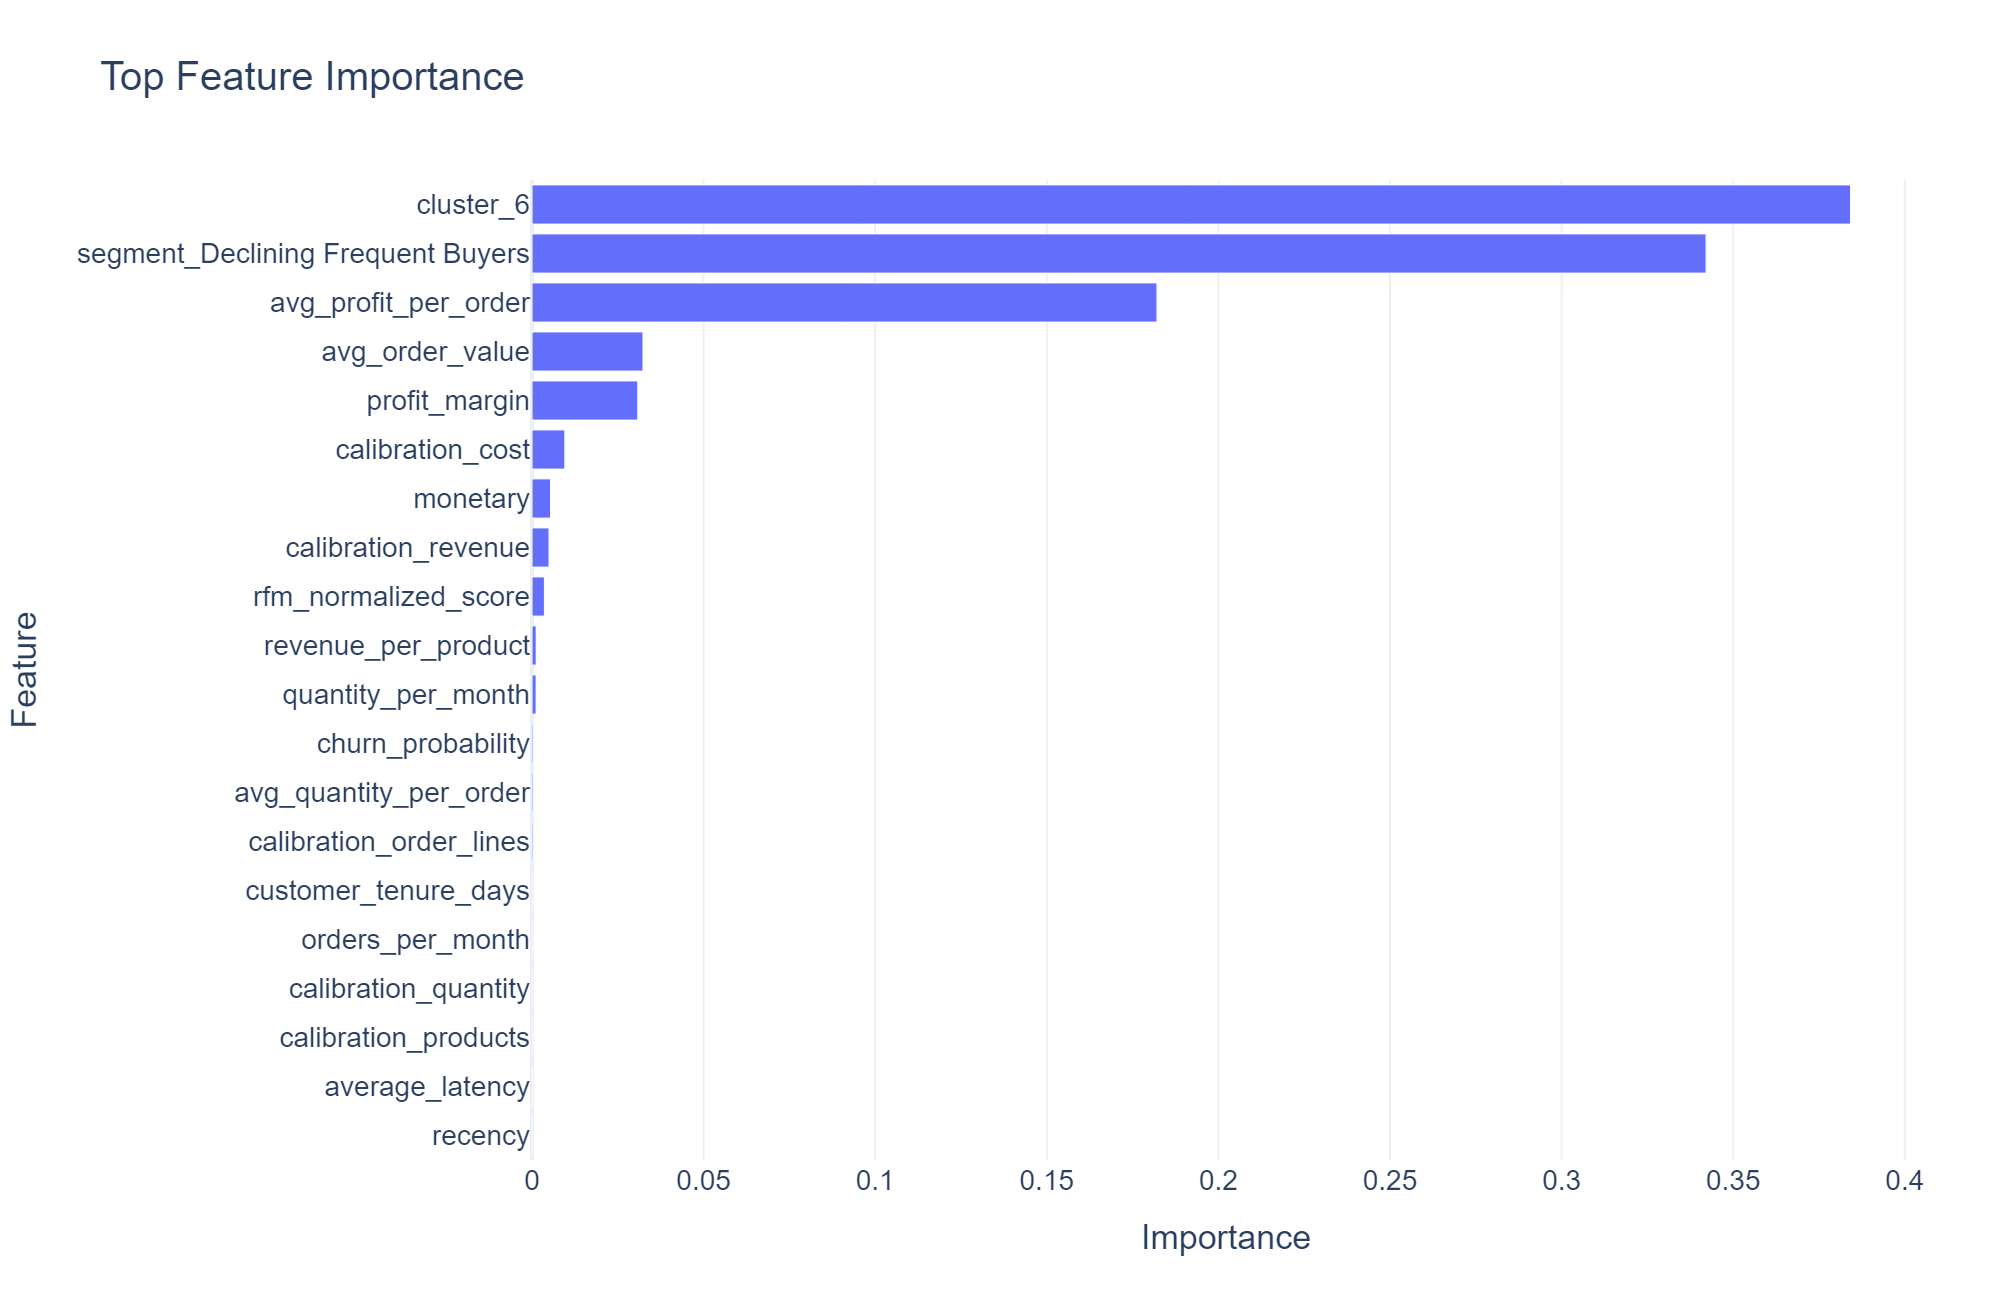
\includegraphics[keepaspectratio]{2-retail-analytics/../notebooks-and-scripts/2-retail-analytics/2-customer-value-and-retention/python/3-customer-value-and-retention-clv-figures/feature-importance.png}}

}

\caption{\label{fig-clv-feature-importance}Feature importance for the
selected Customer Lifetime Value model.}

\end{figure}%

The segment-level results in Table~\ref{tbl-clv-segment-summary} show
why customer value should not be interpreted only at the individual
level. Some segments contribute strongly because they contain many
customers, while others contribute through high average expected value.
The largest aggregate predicted value is concentrated in Declining
Frequent Buyers, mainly because this segment combines a large customer
base with a very high average predicted CLV. By contrast, Lost Customers
and Inactive Low-Value Customers produce negative expected value under
the adopted framework, reflecting weak profitability and unfavourable
behavioural assumptions.

\begin{longtable}[]{@{}
  >{\centering\arraybackslash}p{(\linewidth - 6\tabcolsep) * \real{0.3659}}
  >{\raggedleft\arraybackslash}p{(\linewidth - 6\tabcolsep) * \real{0.1341}}
  >{\centering\arraybackslash}p{(\linewidth - 6\tabcolsep) * \real{0.2439}}
  >{\centering\arraybackslash}p{(\linewidth - 6\tabcolsep) * \real{0.2561}}@{}}
\caption{Customer Lifetime Value summarised by behavioural
segment.}\label{tbl-clv-segment-summary}\tabularnewline
\toprule\noalign{}
\begin{minipage}[b]{\linewidth}\centering
Segment
\end{minipage} & \begin{minipage}[b]{\linewidth}\raggedleft
Customers
\end{minipage} & \begin{minipage}[b]{\linewidth}\centering
Avg. Predicted CLV
\end{minipage} & \begin{minipage}[b]{\linewidth}\centering
Total Predicted CLV
\end{minipage} \\
\midrule\noalign{}
\endfirsthead
\toprule\noalign{}
\begin{minipage}[b]{\linewidth}\centering
Segment
\end{minipage} & \begin{minipage}[b]{\linewidth}\raggedleft
Customers
\end{minipage} & \begin{minipage}[b]{\linewidth}\centering
Avg. Predicted CLV
\end{minipage} & \begin{minipage}[b]{\linewidth}\centering
Total Predicted CLV
\end{minipage} \\
\midrule\noalign{}
\endhead
\bottomrule\noalign{}
\endlastfoot
Declining Frequent Buyers & 1395 & 76859.60 & 107219140.34 \\
High Value but Cooling & 454 & 11367.20 & 5160706.87 \\
Frequent Low-Spend Customers & 928 & 10412.29 & 9662602.51 \\
Active Minimal Buyers & 1767 & 10098.15 & 17843434.86 \\
Inactive Minimal Buyers & 686 & 2776.18 & 1904456.08 \\
Recent Low-Value Customers & 609 & 2748.03 & 1673548.64 \\
Champions & 41 & 242.58 & 9945.82 \\
Lost Customers & 53 & -71046.79 & -3765480.03 \\
Inactive Low-Value Customers & 273 & -18539.27 & -5061219.47 \\
\end{longtable}

These differences are also visible in Figure~\ref{fig-clv-by-segment}
and Figure~\ref{fig-total-clv-by-segment}. The first figure shows the
distribution of predicted CLV within each behavioural segment, while the
second aggregates predicted value across the customer portfolio.
Together, they show that customer prioritisation should consider both
individual-level value and the broader segment structure in which that
value is concentrated.

\begin{figure}

\centering{

\pandocbounded{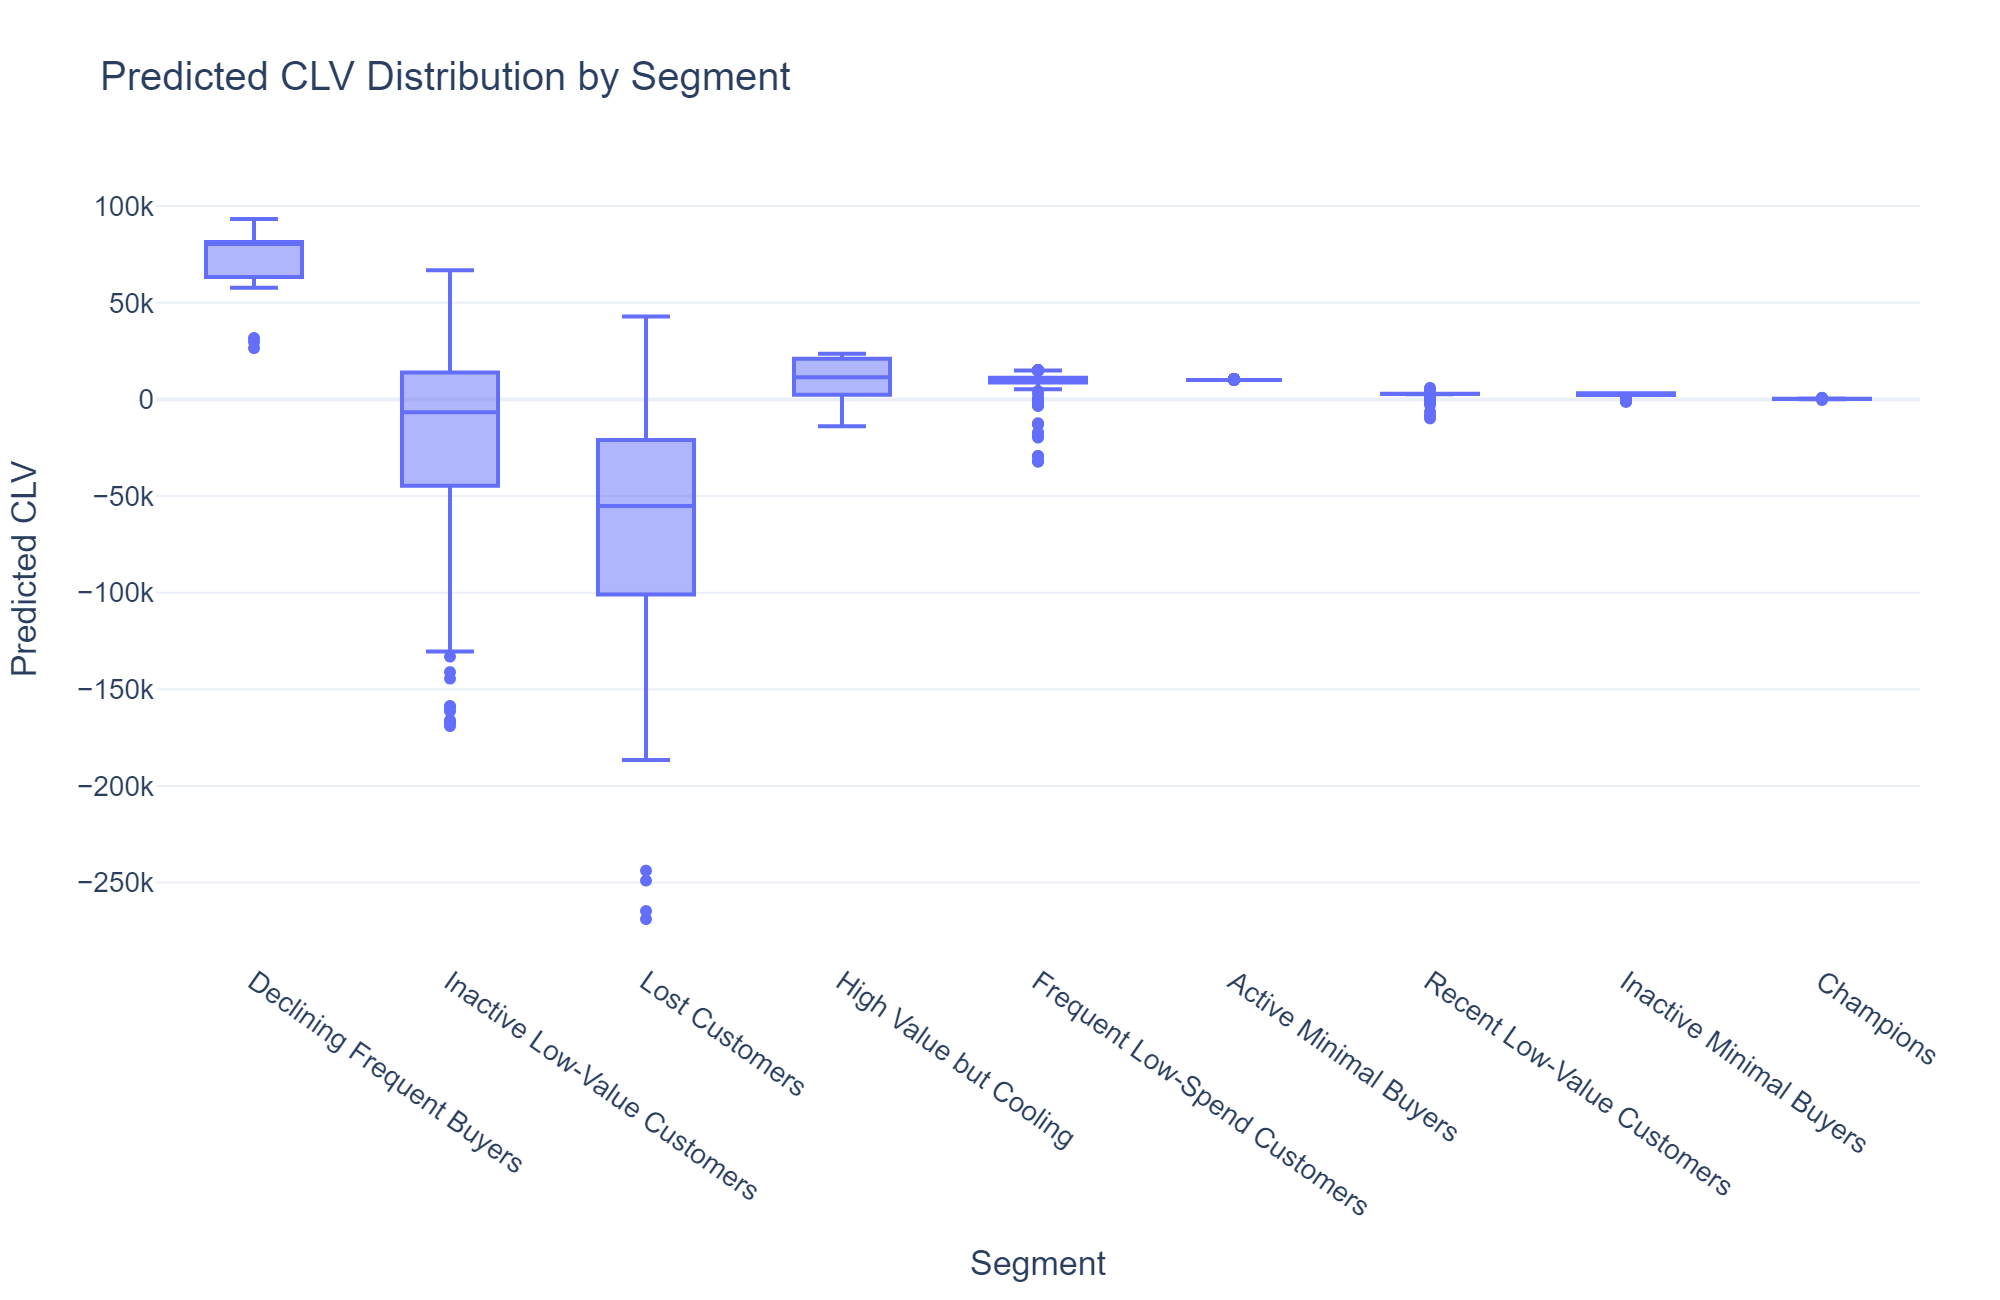
\includegraphics[keepaspectratio]{2-retail-analytics/../notebooks-and-scripts/2-retail-analytics/2-customer-value-and-retention/python/3-customer-value-and-retention-clv-figures/predicted-clv-by-segment.png}}

}

\caption{\label{fig-clv-by-segment}Distribution of predicted Customer
Lifetime Value across customer segments.}

\end{figure}%

\begin{figure}

\centering{

\pandocbounded{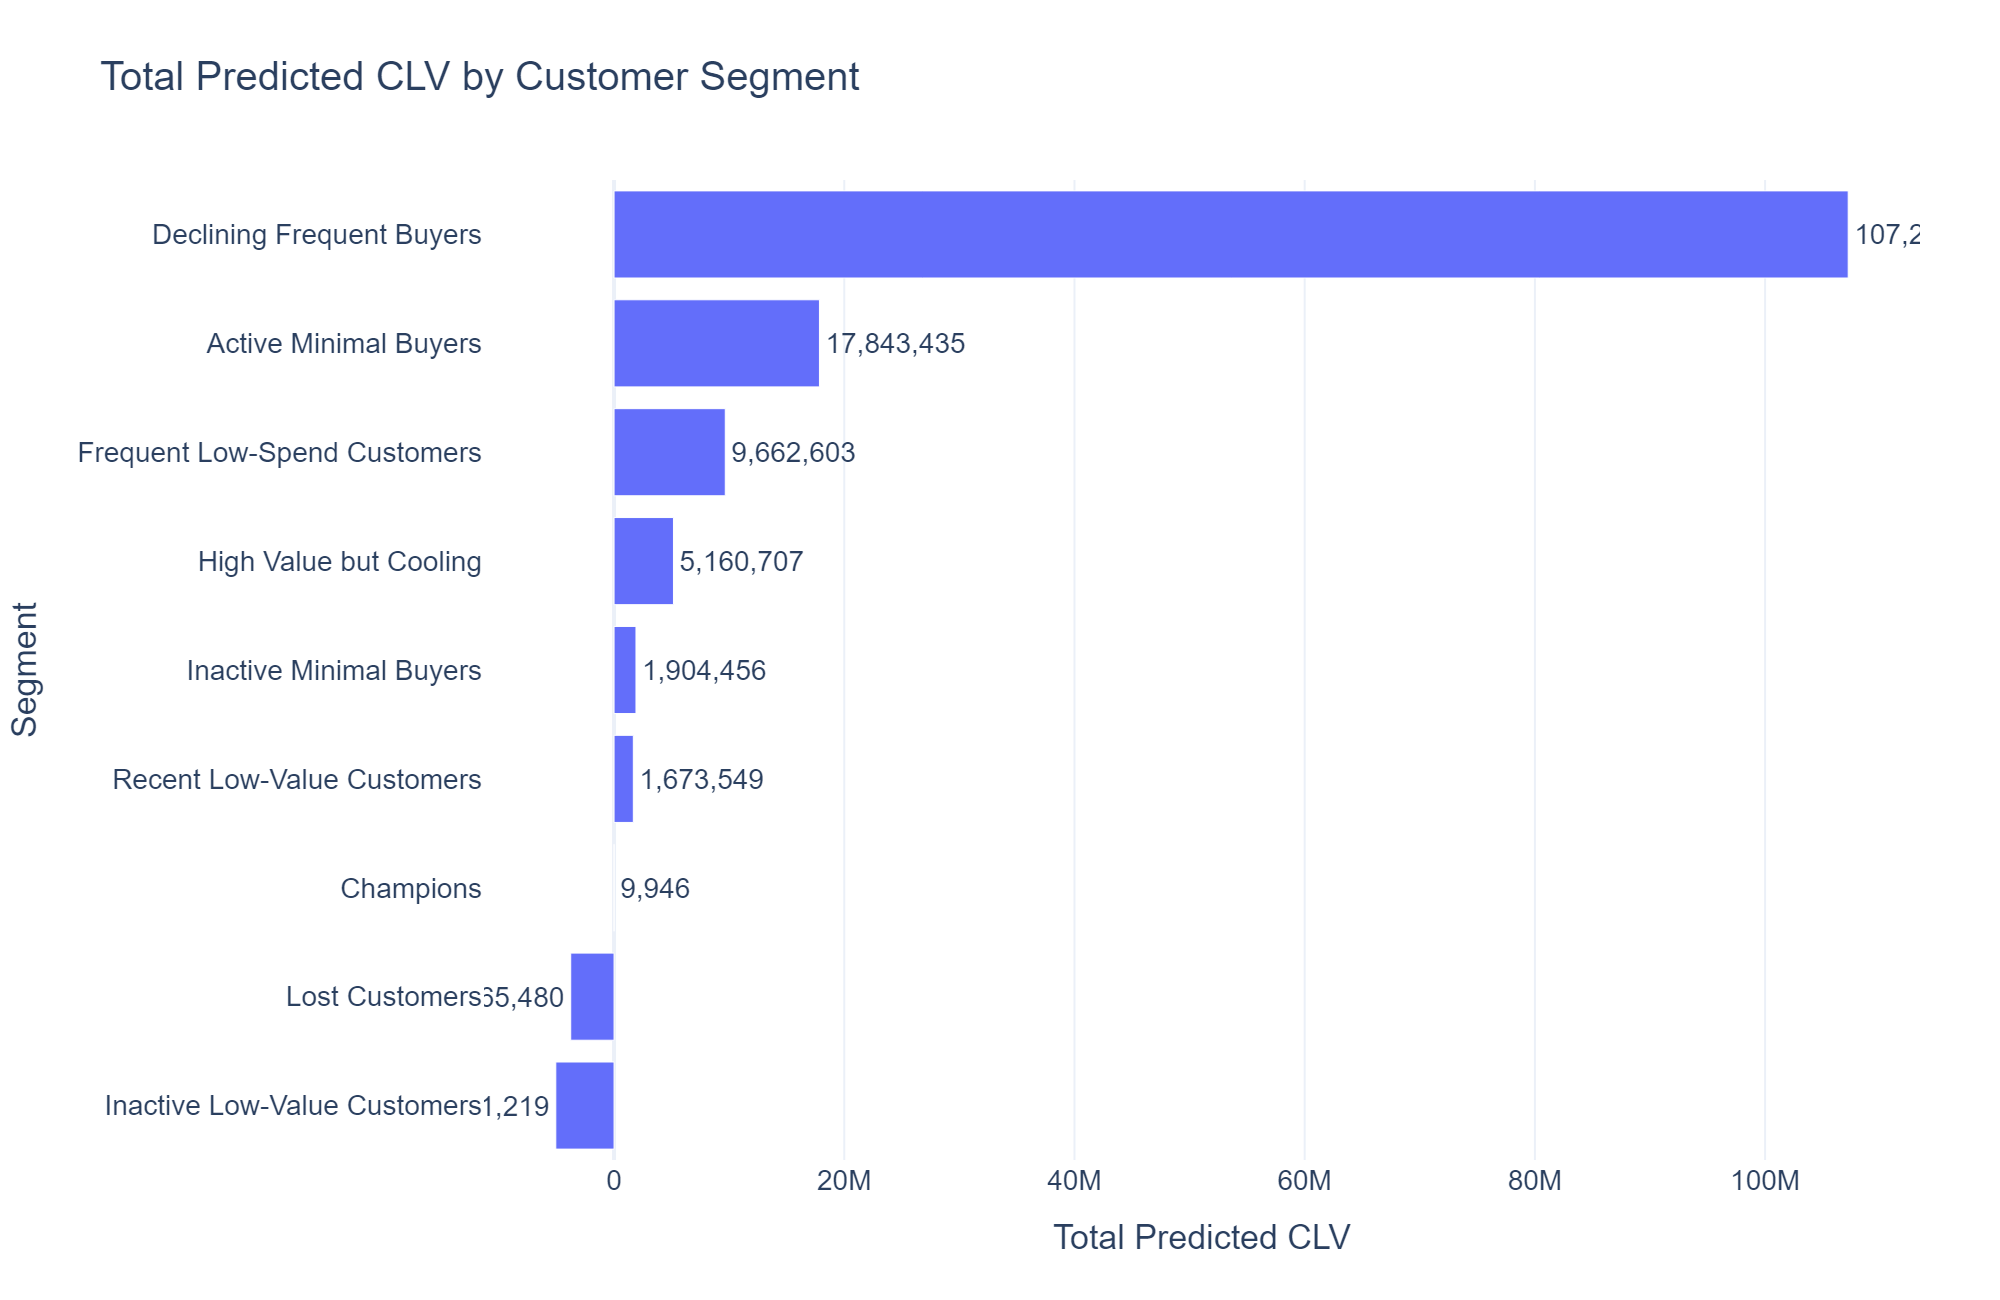
\includegraphics[keepaspectratio]{2-retail-analytics/../notebooks-and-scripts/2-retail-analytics/2-customer-value-and-retention/python/3-customer-value-and-retention-clv-figures/total-predicted-clv-by-segment.png}}

}

\caption{\label{fig-total-clv-by-segment}Total predicted Customer
Lifetime Value aggregated by customer segment.}

\end{figure}%

These results should be interpreted within the assumptions adopted to
construct the valuation framework. The response variable used for model
training is not directly observed in the AdventureWorks database but is
derived from historical profitability, behavioural segmentation,
predicted retention, and explicit discount-rate assumptions.
Consequently, the regression model should be understood as learning to
approximate this internally consistent valuation framework rather than
predicting an objectively measurable quantity. Alternative assumptions
regarding customer retention or discounting would naturally produce
different numerical estimates, although the overall modelling framework
would remain unchanged.

\section{Technical Appendix
(Optional)}\label{technical-appendix-optional-3}

The main chapter emphasises the practical application of customer
analytics using transactional retail data. This appendix complements the
discussion by summarising the principal mathematical concepts underlying
the implementation. Rather than providing exhaustive theoretical
derivations, it introduces the core formulations used throughout the
workflow, including behavioural customer segmentation, the operational
definition of churn, and the construction of the risk-adjusted Customer
Lifetime Value (CLV) framework.

\subsection{RFM Analysis}\label{rfm-analysis}

Recency, Frequency, and Monetary (RFM) analysis is one of the most
widely used approaches for summarising customer purchasing behaviour in
transactional businesses. Instead of modelling the complete purchase
history, it represents each customer through three complementary
behavioural variables:

\begin{itemize}
\tightlist
\item
  \textbf{Recency}, measuring the time elapsed since the customer's most
  recent purchase.
\item
  \textbf{Frequency}, representing the total number of completed
  purchases during the observation period.
\item
  \textbf{Monetary value}, describing the customer's cumulative
  spending.
\end{itemize}

For customer \(i\), Recency is computed as

\begin{equation}\phantomsection\label{eq-rfm-recency}{
R_i=t_{\mathrm{ref}}-t_{\mathrm{last},i},
}\end{equation}

where \(t_{\mathrm{ref}}\) denotes the reference date used for the
analysis and \(t_{\mathrm{last},i}\) is the date of the customer's most
recent transaction.

Frequency is defined as

\begin{equation}\phantomsection\label{eq-rfm-frequency}{
F_i=n_i,
}\end{equation}

where \(n_i\) is the number of completed purchases.

Monetary value is calculated as

\begin{equation}\phantomsection\label{eq-rfm-monetary}{
M_i=\sum_{j=1}^{n_i}v_{ij},
}\end{equation}

where \(v_{ij}\) represents the monetary value of transaction \(j\).

Although conceptually simple, these three variables capture
complementary aspects of customer behaviour and provide the behavioural
representation used throughout the remainder of the workflow. Because
Frequency and Monetary value typically exhibit strong positive skewness,
additional preprocessing is required before applying distance-based
clustering algorithms.

\subsubsection{Box-Cox Transformation}\label{box-cox-transformation}

The RFM variables exhibit markedly different distributions, with
Frequency and Monetary value generally dominated by a relatively small
number of high-value observations. Since K-Means relies on Euclidean
distances, these extreme values can disproportionately influence the
clustering process.

To reduce this effect, each RFM variable is transformed using the
Box-Cox transformation,

\begin{equation}\phantomsection\label{eq-boxcox}{
y^{(\lambda)}=
\begin{cases}
\dfrac{y^\lambda-1}{\lambda}, & \lambda \neq 0,\\
\log(y), & \lambda=0,
\end{cases}
}\end{equation}

where the transformation parameter \(\lambda\) is estimated from the
observed data.

After transformation, each variable is standardised to zero mean and
unit variance before clustering. The transformed variables are used
exclusively during model fitting; all business interpretation remains
based on the original RFM variables.

\subsubsection{K-Means Clustering}\label{k-means-clustering}

Customer segmentation is performed using the K-Means clustering
algorithm, which partitions customers into \(K\) groups by minimising
the within-cluster sum of squared Euclidean distances,

\begin{equation}\phantomsection\label{eq-kmeans}{
\min_{C_1,\ldots,C_K}
\sum_{k=1}^{K}
\sum_{x_i\in C_k}
\left|x_i-\mu_k\right|^2,
}\end{equation}

where \(\mu_k\) denotes the centroid of cluster \(k\).

The optimisation alternates between assigning observations to their
nearest centroid and updating the centroids according to the mean of the
assigned observations until convergence.

Since no ground-truth customer labels exist, the optimal number of
clusters is determined using complementary internal validation metrics
together with business interpretability. Once the clusters have been
identified, they are interpreted using the original RFM variables rather
than the transformed feature space, allowing each segment to be
associated with a meaningful purchasing profile.

\subsection{Behavioural Churn
Definition}\label{behavioural-churn-definition}

Unlike subscription-based businesses, transactional retail datasets
rarely contain explicit churn events. Customer inactivity must therefore
be inferred from observed purchasing behaviour rather than directly
measured. The implementation adopted in this project defines churn
through a behavioural rule that combines customer engagement during the
calibration period with observed activity during a subsequent validation
period.

Let \(S_i\) denote the behavioural segment assigned to customer \(i\),
\(R_i\) the customer's recency, \(\bar{L}_i\) the average time between
consecutive purchases (purchase latency), and \(\mathrm{Score}_i\) the
within-segment RFM score. Furthermore, let
\(\overline{\mathrm{Score}}_{S_i}\) represent the average RFM score of
the customer's segment.

A customer is considered a potential churn candidate when all
behavioural conditions

\[
S_i\in\mathcal{L},
\]

\[
R_i>\bar{L}_i,
\]

and

\[
\mathrm{Score}_i<
\overline{\mathrm{Score}}_{S_i}
\]

are simultaneously satisfied, where \(\mathcal{L}\) denotes the set of
low-activity customer segments identified during the RFM analysis.

The final churn label is then determined by inspecting future purchasing
behaviour during the validation period,

\begin{equation}\phantomsection\label{eq-churn-definition}{
y_i=
\begin{cases}
1, & \text{if the customer makes no purchases during the validation window},\\
0, & \text{otherwise}.
\end{cases}
}\end{equation}

This formulation differs from the common approach of defining churn
solely through future inactivity. Instead, it first identifies customers
whose historical purchasing behaviour is already consistent with
progressive disengagement and subsequently verifies whether this
behaviour persists during the validation period. By separating
behavioural identification from future validation, the resulting target
remains suitable for supervised learning while reducing the risk of
labelling temporarily inactive customers as permanent churners.

The chronological separation between calibration and validation periods
also prevents information leakage, since every explanatory variable is
computed exclusively from information that would have been available at
the time the prediction is made.

\subsubsection{Classification Metrics}\label{classification-metrics}

Customer churn prediction is formulated as a binary classification
problem. Let

\begin{itemize}
\tightlist
\item
  \(TP\): true positives,
\item
  \(FP\): false positives,
\item
  \(TN\): true negatives,
\item
  \(FN\): false negatives.
\end{itemize}

Several complementary metrics are used throughout the chapter to
evaluate predictive performance.

Precision measures the proportion of customers predicted to churn who
actually become inactive,

\begin{equation}\phantomsection\label{eq-precision}{
\mathrm{Precision}
=
\frac{TP}{TP+FP},
}\end{equation}

where higher values indicate fewer false positive predictions.

Recall, also referred to as sensitivity, measures the proportion of
actual churners correctly identified by the classifier,

\begin{equation}\phantomsection\label{eq-recall}{
\mathrm{Recall}
=
\frac{TP}{TP+FN},
}\end{equation}

making it particularly relevant when missing high-risk customers carries
a significant commercial cost.

The harmonic mean of Precision and Recall is given by the F1-score,

\begin{equation}\phantomsection\label{eq-f1}{
F_1
=
2
\cdot
\frac{\mathrm{Precision}\times\mathrm{Recall}}
{\mathrm{Precision}+\mathrm{Recall}},
}\end{equation}

which provides a balanced summary of classifier performance under class
imbalance.

Threshold-independent evaluation is performed using the Receiver
Operating Characteristic (ROC) curve and the Precision--Recall curve.
While ROC analysis measures the trade-off between the true positive rate
and false positive rate across all possible classification thresholds,
Precision--Recall curves provide a more informative assessment when the
positive class is relatively uncommon, as is typically the case in
customer retention problems.

From a business perspective, ranking quality is often more important
than binary classification accuracy. For this reason, the implementation
also evaluates cumulative gains, which quantify how effectively the
model concentrates future churners within the highest-ranked customers.
This ranking perspective is particularly useful for prioritising
retention campaigns when marketing resources are limited.

\subsection{Risk-Adjusted Customer Lifetime
Value}\label{risk-adjusted-customer-lifetime-value}

Customer Lifetime Value (CLV) is commonly defined as the present value
of the future profits expected from a customer relationship. A general
formulation is given by

\begin{equation}\phantomsection\label{eq-classical-clv}{
\mathrm{CLV}
=
\sum_{t=1}^{T}
\frac{\mathbb{E}[P_t]}
{(1+d)^t},
}\end{equation}

where \(\mathbb{E}[P_t]\) denotes the expected customer profit during
period \(t\), \(d\) is the discount rate, and \(T\) represents the
planning horizon.

In practice, however, neither future profits nor customer retention are
directly observable in non-contractual retail businesses. The
implementation presented in this chapter therefore constructs a
risk-adjusted valuation framework that combines observed customer
profitability with behavioural information derived from the previous
stages of the workflow.

Let \(\hat{P}_i\) denote the estimated average profit generated by
customer \(i\), \(c_{S_i}\) the historical churn rate associated with
the behavioural segment (S\_i), and (d\_\{S\_i\}) the corresponding
segment-specific discount rate. Assuming that the probability of
customer retention remains approximately constant within each
behavioural segment, the expected Customer Lifetime Value is estimated
as

\begin{equation}\phantomsection\label{eq-risk-adjusted-clv}{
\widehat{\mathrm{CLV}}_i
=
\sum_{t=1}^{T}
\frac{
\hat{P}_i
\left(1-c_{S_i}\right)^{t-1}
}
{\left(1+d_{S_i}\right)^t},
}\end{equation}

where the term

\[
\left(1-c_{S_i}\right)^{t-1}
\]

represents the probability that customer \(i\) remains active up to
period \(t\).

Unlike the classical formulation, both the expected retention and the
discount rate depend on the customer's behavioural segment rather than
being assumed identical across the entire customer base. This allows
customers exhibiting different purchasing patterns to be valued under
different behavioural assumptions while preserving a transparent and
reproducible valuation framework.

The resulting quantity should not be interpreted as an objectively
measurable future lifetime value. Instead, it represents a model-based
valuation constructed from observed profitability together with explicit
assumptions regarding customer retention and the time value of money.

Once the target variable has been constructed, Customer Lifetime Value
prediction becomes a supervised regression problem,

\begin{equation}\phantomsection\label{eq-clv-regression}{
\widehat{\mathrm{CLV}}_i
=
f(\mathbf{x}_i)+\varepsilon_i,
}\end{equation}

where \(\mathbf{x}_i\) denotes the customer-level feature vector
engineered throughout the project, \(f(\cdot)\) represents the
regression model, and \(\varepsilon_i\) captures the unexplained
prediction error.

Rather than estimating future profits directly, the regression model
learns to approximate the valuation framework defined by
Equation~\ref{eq-risk-adjusted-clv}. This considerably reduces the
computational effort required to evaluate new customers while
maintaining consistency with the behavioural and financial assumptions
adopted throughout the analytical workflow.

\chapter{Customer Sentiment and Topic
Analysis}\label{customer-sentiment-and-topic-analysis}

\emph{Header.}

\section{Problem Definition}\label{problem-definition-5}

\emph{Section.}

\section{Modeling Approach}\label{modeling-approach-5}

\emph{Section.}

\section{Methodology and
Implementation}\label{methodology-and-implementation-5}

\emph{Section.}

\section{Results, Discussion, and
Limitations}\label{results-discussion-and-limitations-5}

\emph{Section.}

\section{Technical Appendix
(Optional)}\label{technical-appendix-optional-4}

\emph{Section.}

\part{Biological Systems}

\chapter*{Overview}\label{overview-2}
\addcontentsline{toc}{chapter}{Overview}

\markboth{Overview}{Overview}

This part covers problems related to biological systems, including the
analysis and modeling of data arising in biological, health, and life
science contexts.

The scope of this domain includes approaches for studying complex
processes, identifying patterns in biological data, and supporting
analysis in settings where systems are often heterogeneous, nonlinear,
and influenced by multiple interacting factors.

\chapter{Predicting Crop Performance from Soil Microbial
Communities}\label{predicting-crop-performance-from-soil-microbial-communities}

\emph{Header.}

\section{Problem Definition}\label{problem-definition-6}

\emph{Section.}

\section{Modeling Approach}\label{modeling-approach-6}

\emph{Section.}

\section{Methodology and
Implementation}\label{methodology-and-implementation-6}

\emph{Section.}

\section{Results, Discussion, and
Limitations}\label{results-discussion-and-limitations-6}

\emph{Section.}

\section{Technical Appendix
(Optional)}\label{technical-appendix-optional-5}

\emph{Section.}

\chapter{Medical Image Analysis for Skin Lesion
Triage}\label{medical-image-analysis-for-skin-lesion-triage}

\emph{Header.}

\section{Problem Definition}\label{problem-definition-7}

\emph{Section.}

\section{Modeling Approach}\label{modeling-approach-7}

\emph{Section.}

\section{Methodology and
Implementation}\label{methodology-and-implementation-7}

\emph{Section.}

\section{Results, Discussion, and
Limitations}\label{results-discussion-and-limitations-7}

\emph{Section.}

\section{Technical Appendix
(Optional)}\label{technical-appendix-optional-6}

\emph{Section.}

\part{Energy and Industrial Systems}

\chapter*{Overview}\label{overview-3}
\addcontentsline{toc}{chapter}{Overview}

\markboth{Overview}{Overview}

This part covers problems related to energy and industrial systems,
including the analysis and modeling of production processes, physical
assets, and operational data.

The scope of this domain includes approaches for optimization and
efficient resource allocation, monitoring and analysis of system
integrity, and the study of degradation processes such as corrosion, as
well as data-driven methods to support decision-making in complex
operational environments.

\chapter{Permeability Prediction in Porous
Media}\label{permeability-prediction-in-porous-media}

\emph{Header.}

\section{Problem Definition}\label{problem-definition-8}

\emph{Section.}

\section{Modeling Approach}\label{modeling-approach-8}

\emph{Section.}

\section{Methodology and
Implementation}\label{methodology-and-implementation-8}

\emph{Section.}

\section{Results, Discussion, and
Limitations}\label{results-discussion-and-limitations-8}

\emph{Section.}

\section{Technical Appendix
(Optional)}\label{technical-appendix-optional-7}

\emph{Section.}

\chapter{Predicting Pipeline Corrosion for Asset Integrity
Management}\label{predicting-pipeline-corrosion-for-asset-integrity-management}

\emph{Header.}

\section{Problem Definition}\label{problem-definition-9}

\emph{Section.}

\section{Modeling Approach}\label{modeling-approach-9}

\emph{Section.}

\section{Methodology and
Implementation}\label{methodology-and-implementation-9}

\emph{Section.}

\section{Results, Discussion, and
Limitations}\label{results-discussion-and-limitations-9}

\emph{Section.}

\section{Technical Appendix
(Optional)}\label{technical-appendix-optional-8}

\emph{Section.}

\part{Climate and Environmental Systems}

\chapter*{Overview}\label{overview-4}
\addcontentsline{toc}{chapter}{Overview}

\markboth{Overview}{Overview}

This part covers problems related to climate and environmental systems,
including the analysis and modeling of temporal and spatial data
describing atmospheric and large-scale natural processes.

The scope of this domain includes approaches for time series analysis,
forecasting, and the study of variability and uncertainty in systems
influenced by natural dynamics, external drivers, and interactions
across multiple scales.

\chapter{Sediment Source Modeling}\label{sediment-source-modeling}

Sediment source apportionment aims to estimate how much each potential
source contributes to the sediment collected at a downstream location.
The problem arises in watershed management, erosion assessment, and
river restoration, where understanding the origin of transported
sediments is often more important than simply measuring their volume.

This project compares three complementary source apportionment
approaches using laboratory mixtures with known compositions and
synthetic mixtures generated from the same experimental dataset.
Alongside a probabilistic fingerprinting model, two deterministic
geochemical deconvolution algorithms originally developed for petroleum
production allocation are adapted to sediment source apportionment,
allowing their performance to be evaluated under controlled conditions.

\section{Problem Definition}\label{problem-definition-10}

Sediments transported through a watershed are typically generated by
multiple erosion processes acting simultaneously. Agricultural fields,
forested areas, channel banks, and other landscape units may all
contribute material to the sediment ultimately deposited downstream.
Although the resulting mixture can be sampled directly, the relative
contribution of each source cannot be measured independently, making
source apportionment an inverse problem.

A common strategy is to characterize each potential source using a set
of geochemical tracers and compare these fingerprints with those
measured in the collected sediment. If the selected tracers are
sufficiently discriminative, the observed composition can be interpreted
as the result of combining material from multiple sources in unknown
proportions. The objective is therefore to estimate a vector of source
proportions that reproduces the measured composition while satisfying
the physical constraints of the mixing process.

The overall source apportionment workflow is illustrated in
Figure~\ref{fig-sediment-source-apportionment-workflow}. Representative
geochemical signatures are first collected from potential sediment
sources, which subsequently mix during erosion, transport, and
deposition. After sampling and laboratory analysis, the measured
composition is used to estimate the relative contribution of each source
to the final mixture.

\begin{figure}

\centering{

\pandocbounded{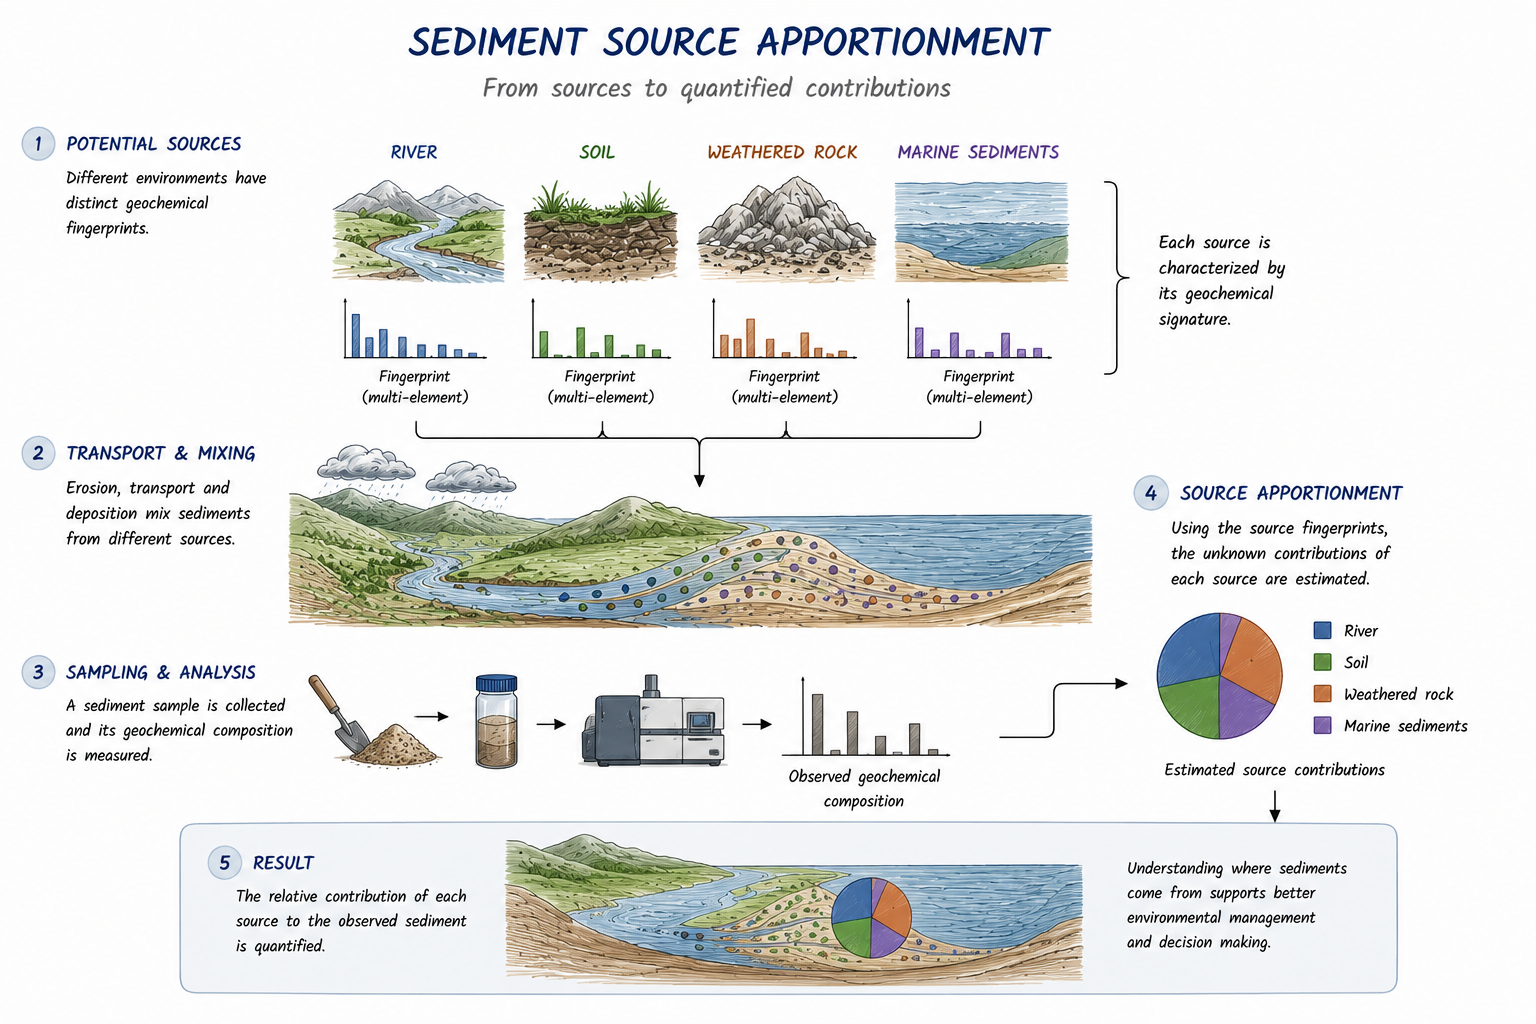
\includegraphics[keepaspectratio]{5-climate-and-environmental-systems/figures/sediment-source-apportionment-workflow.png}}

}

\caption{\label{fig-sediment-source-apportionment-workflow}Conceptual
workflow of sediment source apportionment. Representative geochemical
fingerprints are measured for potential sediment sources, transported
and mixed within the watershed, and subsequently used to estimate the
relative contribution of each source to an observed sediment sample.}

\end{figure}%

Several factors make this estimation challenging. Geochemical signatures
from different sources often overlap, laboratory measurements are
subject to analytical uncertainty, and the number of available tracers
is usually limited. Moreover, the estimated source proportions must
remain non-negative and sum to one, introducing additional constraints
that distinguish the problem from an unconstrained regression task.

One of the main difficulties when assessing source apportionment methods
is that the true source proportions are rarely known for field
observations. As a result, performance is often evaluated indirectly
through sensitivity analyses or expert interpretation. To overcome this
limitation, Batista, Laceby, and Evrard
\citeproc{ref-batista2022evaluate}{{[}30{]}} proposed an experimental
framework based on laboratory-prepared sediment mixtures with known
source proportions. Because the true composition of each mixture is
available, different modelling approaches can be evaluated objectively
using quantitative performance metrics.

This project adopts that experimental framework and compares three
complementary source apportionment methods using the same benchmark
dataset. In addition to the laboratory mixtures, the evaluation also
includes a large collection of synthetic mixtures generated from the
experimental data, allowing model behaviour to be examined over a much
broader range of source combinations while preserving complete knowledge
of the ground truth.

\section{Modeling Approach}\label{modeling-approach-10}

At first glance, sediment fingerprinting and petroleum production
allocation appear to address entirely different scientific problems. The
former seeks to determine the origin of sediments transported through a
watershed, whereas the latter estimates the contribution of individual
reservoirs to a commingled production stream. Despite these differences,
both can be formulated as the same inverse problem: recovering the
proportions of multiple sources from a compositional mixture subject to
physical constraints.

This shared mathematical structure motivated the comparison presented in
this chapter. Rather than proposing a new source apportionment
algorithm, the objective is to evaluate whether deconvolution methods
that have been successfully applied in petroleum geochemistry can also
recover sediment source proportions from environmental fingerprinting
data. Laboratory-prepared mixtures with known compositions provide an
ideal benchmark because every prediction can be compared directly with
the true proportions.

The first method considered is the Bootstrapped Mixing Model (BMM)
described by Batista, Laceby, and Evrard
\citeproc{ref-batista2022evaluate}{{[}30{]}}. This probabilistic
framework repeatedly resamples the geochemical observations to propagate
measurement variability through the mixing model, producing a
distribution of plausible source proportions instead of a single
deterministic estimate. Because it explicitly represents uncertainty,
the BMM serves as a natural reference against which alternative
approaches can be evaluated.

The remaining methods originate from petroleum geochemistry. McCaffrey
et al.~(2011) \citeproc{ref-mccaffrey2011geochemical}{{[}31{]}}
formulated the allocation problem as a constrained least-squares
optimization, estimating the unknown source proportions directly from
elemental concentrations while enforcing non-negativity and mass
conservation. Sandoval et al.~(2022)
\citeproc{ref-sandoval2022original}{{[}32{]}} later extended this idea
by performing the estimation in log-ratio space, an approach
specifically designed for compositional data that mitigates numerical
issues associated with the constant-sum constraint and improves the
treatment of relative geochemical information.

Although neither deterministic model was originally developed for
sediment fingerprinting, both rely on assumptions that remain valid for
conservative geochemical tracers. Consequently, applying them to
sediment source apportionment requires no modification of their
mathematical formulation, only a reinterpretation of what constitutes a
``source.'' In petroleum applications, the sources correspond to
producing reservoirs, whereas in this study they represent
sediment-producing landscape units.

To ensure that differences in performance arise from the modelling
strategies rather than the data themselves, all three methods are
evaluated using exactly the same benchmark datasets. Their estimates are
then compared against the known source proportions, providing a
controlled assessment of accuracy, robustness, and the practical
advantages and limitations of each formulation.

\section{Methodology and
Implementation}\label{methodology-and-implementation-10}

The implementation was organized as three independent workflows, one for
each modelling approach. This separation was intentional: each model
uses a different representation of the mixing problem, different
assumptions about uncertainty, and different diagnostic outputs. Keeping
the workflows independent makes the comparison easier to audit and
avoids forcing the three methods into a single artificial pipeline.

All methods are evaluated using the same sediment fingerprinting dataset
and the same known source proportions. Consequently, any differences in
performance arise from the modelling formulation rather than from
changes in the input data. This distinction is particularly important
because the objective is not only to obtain accurate source
apportionments, but also to understand how each formulation behaves when
applied to the same controlled mixtures.

\subsection{Bootstrapped Mixing Model}\label{bootstrapped-mixing-model}

The Bootstrapped Mixing Model (BMM) serves as the probabilistic baseline
throughout this study. Unlike deterministic mixing models that produce a
single estimate of the source proportions, the BMM propagates
measurement uncertainty through repeated bootstrap resampling. The
result is not only an estimate for each sediment source, but a
distribution of plausible solutions for every mixture.

The implementation follows the evaluation framework proposed by Batista,
Laceby, and Evrard \citeproc{ref-batista2022evaluate}{{[}30{]}}. The
workflow begins by examining the available source fingerprints, then
selects the tracers with the strongest discriminatory power, and finally
estimates the source proportions for both laboratory-prepared and
synthetically generated benchmark mixtures.

A complete Python implementation of the Bootstrapped Mixing Model
presented in this section is available in the project repository
\href{https://github.com/rodrigokang/portfolio/tree/main/notebooks-and-scripts/5-climate-and-environmental-systems/1-sediment-source-modeling}{here}.

\subsubsection{Exploratory Analysis}\label{exploratory-analysis}

Before fitting the mixing model, the source data were inspected to
verify that each sediment class was adequately represented and that the
candidate geochemical tracers carried sufficient discriminatory
information. This step is important because source apportionment depends
on separating source signatures rather than simply reproducing a
numerical mixture.

Figure~\ref{fig-bmm-source-sample-counts} summarizes the number of
samples available for each sediment source. Although the sampling effort
is not perfectly balanced, every class contains enough observations to
characterize source variability and support the bootstrap resampling
procedure.

\begin{figure}

\centering{

\pandocbounded{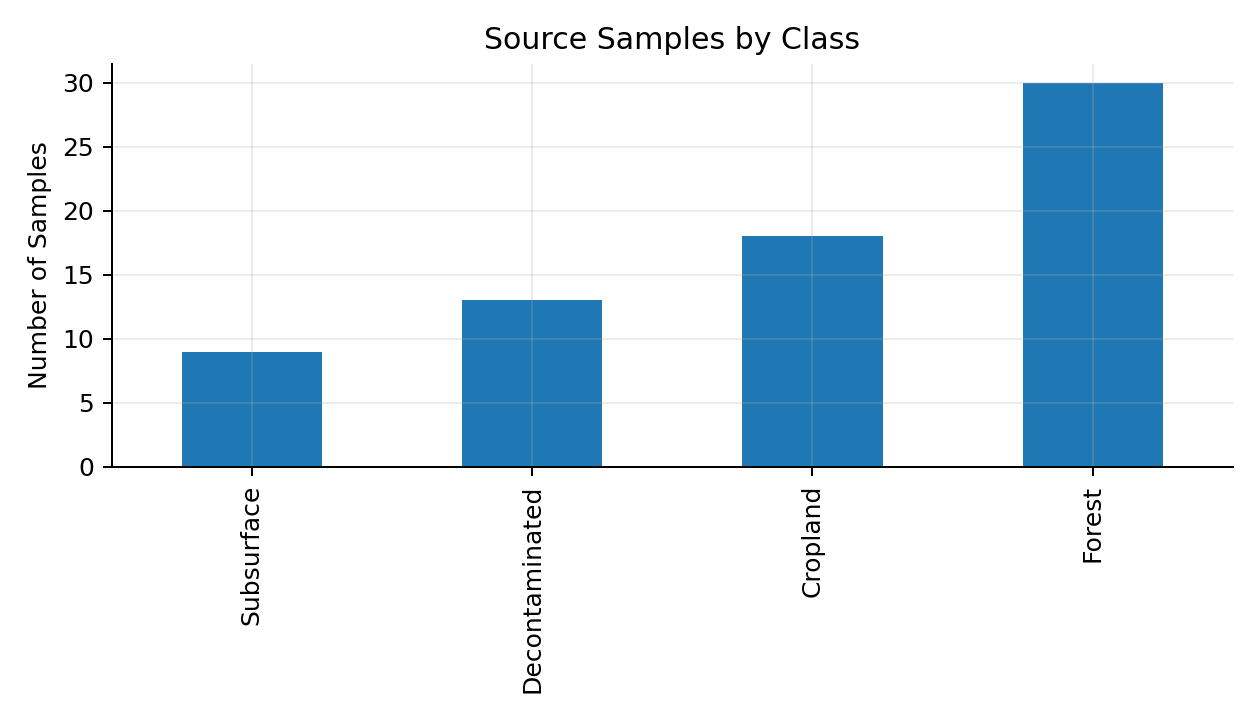
\includegraphics[keepaspectratio]{5-climate-and-environmental-systems/../notebooks-and-scripts/5-climate-and-environmental-systems/1-sediment-source-modeling/python/1-sediment-source-modeling-batista-figures/figures/source_sample_counts.png}}

}

\caption{\label{fig-bmm-source-sample-counts}Number of samples available
for each sediment source.}

\end{figure}%

Candidate tracers were screened using the non-parametric Kruskal--Wallis
test. The retained variables, listed in
Table~\ref{tbl-bmm-selected-tracers}, show statistically significant
differences among the four source classes and were therefore selected
for the subsequent source apportionment analysis.

\begin{longtable}[]{@{}ccc@{}}
\caption{Geochemical tracers retained after Kruskal--Wallis
screening.}\label{tbl-bmm-selected-tracers}\tabularnewline
\toprule\noalign{}
\textbf{Tracer} & \textbf{H Statistic} & \textbf{p-value} \\
\midrule\noalign{}
\endfirsthead
\toprule\noalign{}
\textbf{Tracer} & \textbf{H Statistic} & \textbf{p-value} \\
\midrule\noalign{}
\endhead
\bottomrule\noalign{}
\endlastfoot
L & 51.647 & 3.56e-11 \\
h & 45.480 & 7.32e-10 \\
Si & 43.607 & 1.83e-09 \\
C* & 34.421 & 1.61e-07 \\
K & 33.015 & 3.20e-07 \\
Y & 23.563 & 3.08e-05 \\
Mn & 13.278 & 4.07e-03 \\
Zn & 12.499 & 5.86e-03 \\
Ti & 9.213 & 2.66e-02 \\
\end{longtable}

The selected tracer set was also examined through Linear Discriminant
Analysis. As shown in Figure~\ref{fig-bmm-lda-selected-tracers}, most
source classes occupy distinct regions of the projected feature space,
although some overlap remains. This behaviour is expected in
environmental fingerprinting studies and further supports the use of a
probabilistic framework rather than a purely classificatory approach.

\begin{figure}

\centering{

\pandocbounded{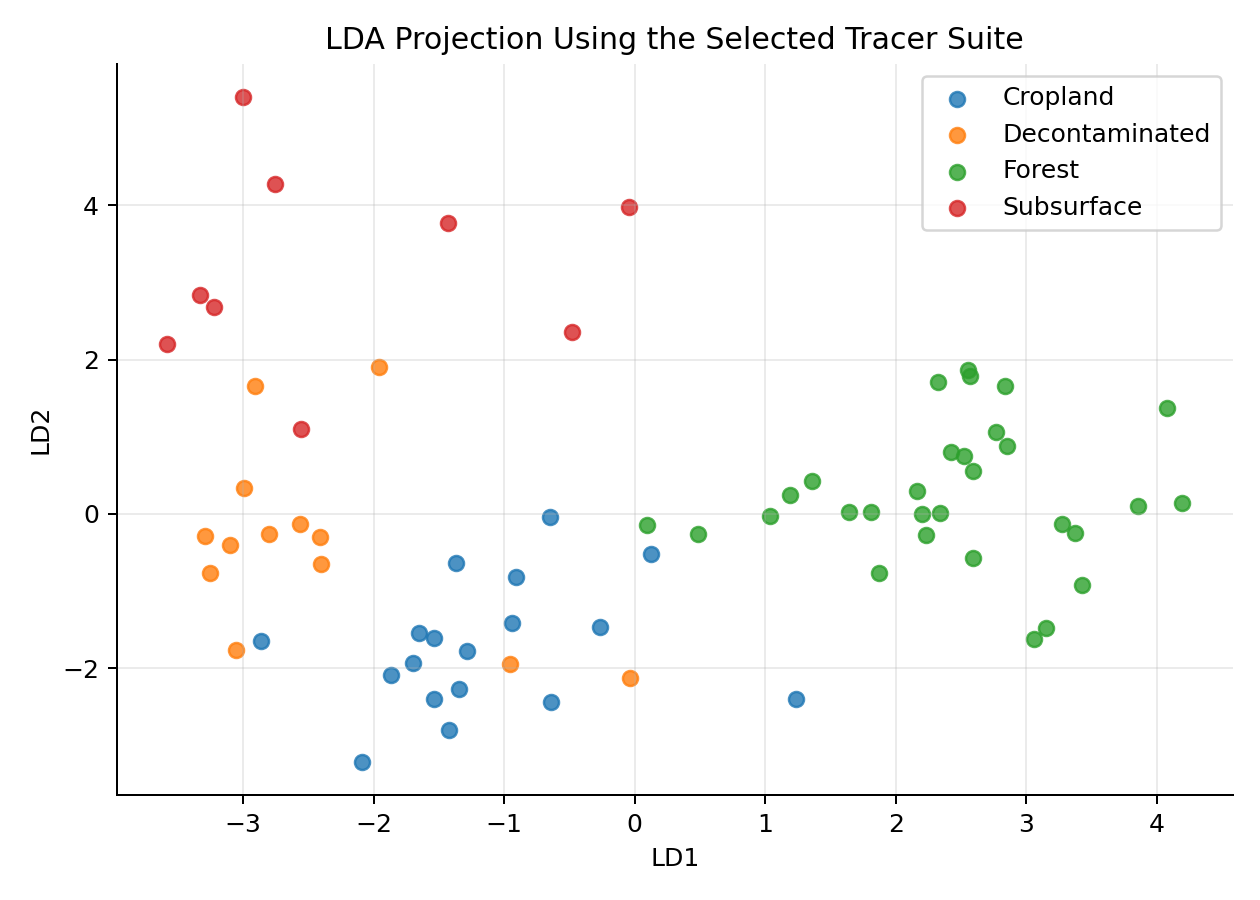
\includegraphics[keepaspectratio]{5-climate-and-environmental-systems/../notebooks-and-scripts/5-climate-and-environmental-systems/1-sediment-source-modeling/python/1-sediment-source-modeling-batista-figures/figures/lda_selected_tracers.png}}

}

\caption{\label{fig-bmm-lda-selected-tracers}Linear Discriminant
Analysis projection using the selected geochemical tracers.}

\end{figure}%

\subsubsection{Source Apportionment}\label{source-apportionment}

The selected tracers were then used to estimate the source proportions
for both the laboratory-prepared and synthetic benchmark mixtures. For
each sample, the BMM returns predictive intervals that quantify the
uncertainty associated with every estimated proportion.

The laboratory results are presented in
Figure~\ref{fig-bmm-laboratory-intervals}. In most cases, the known
source proportions fall within the predicted intervals, indicating that
the model captures the main structure of the mixing process while
appropriately representing the uncertainty arising from overlapping
source fingerprints.

\begin{figure}

\centering{

\pandocbounded{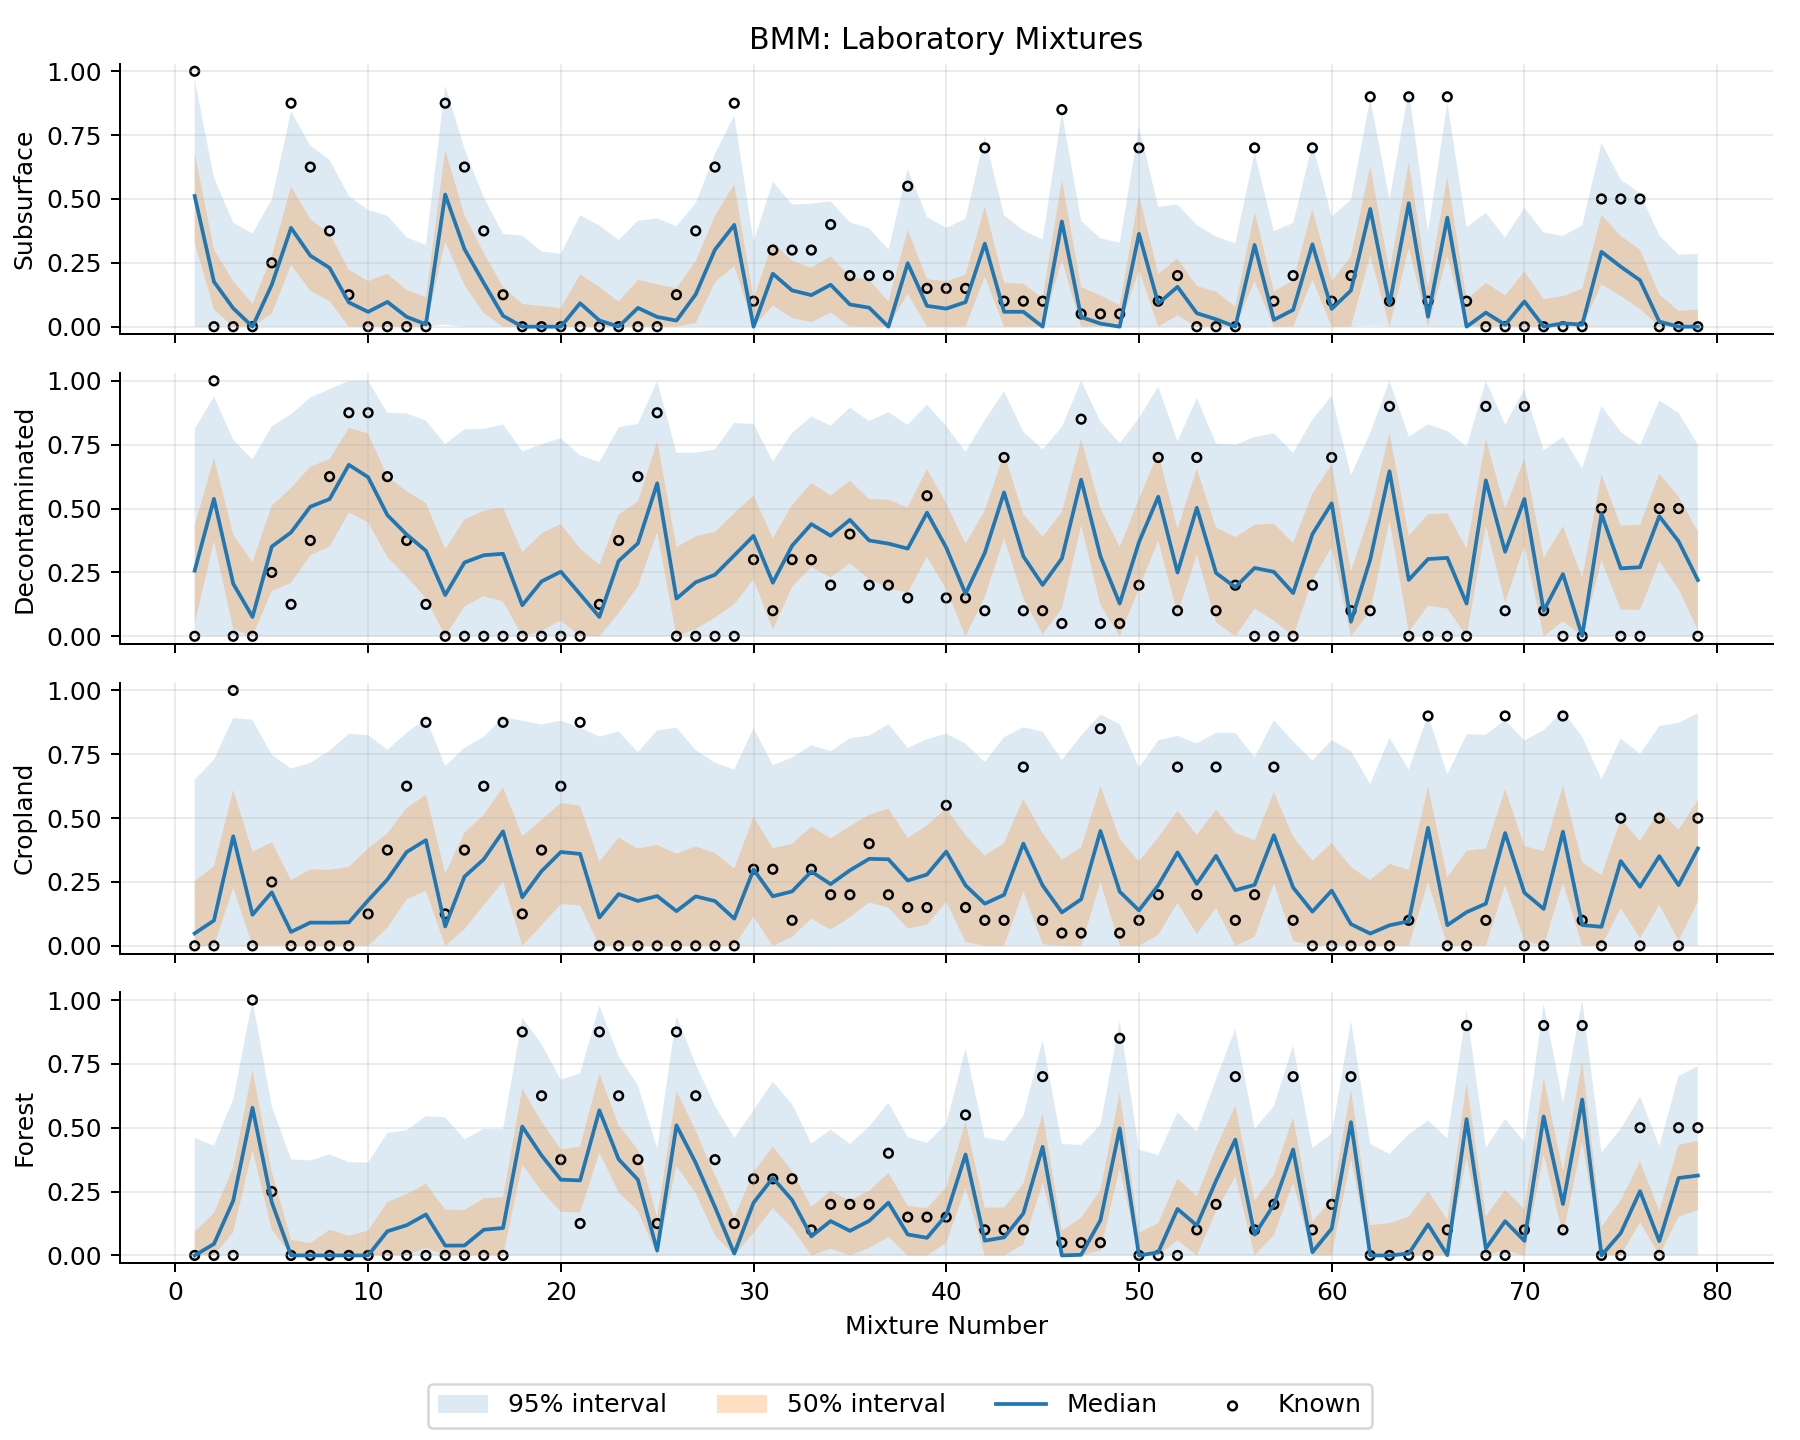
\includegraphics[keepaspectratio]{5-climate-and-environmental-systems/../notebooks-and-scripts/5-climate-and-environmental-systems/1-sediment-source-modeling/python/1-sediment-source-modeling-batista-figures/figures/intervals_bmm_laboratory.png}}

}

\caption{\label{fig-bmm-laboratory-intervals}Predicted source
contributions for the laboratory-prepared mixtures using the
Bootstrapped Mixing Model.}

\end{figure}%

The same procedure was subsequently applied to the synthetic benchmark.
As shown in Figure~\ref{fig-bmm-laboratory-vs-virtual}, predictive
performance improves substantially when evaluated on these mixtures,
which provide a more systematic coverage of the compositional space than
the smaller laboratory dataset.

\begin{figure}

\centering{

\pandocbounded{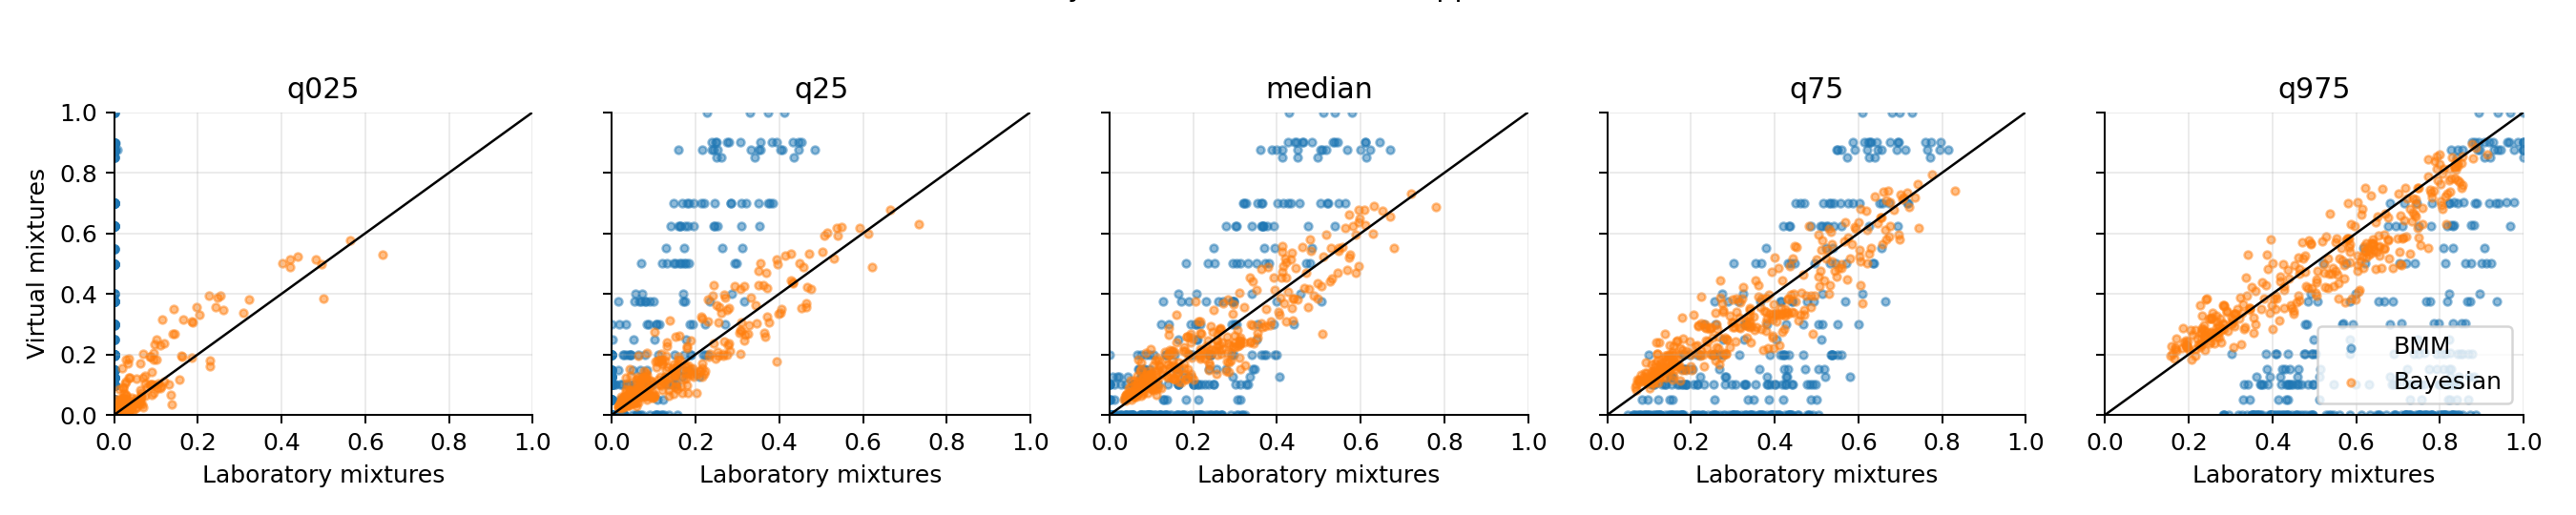
\includegraphics[keepaspectratio]{5-climate-and-environmental-systems/../notebooks-and-scripts/5-climate-and-environmental-systems/1-sediment-source-modeling/python/1-sediment-source-modeling-batista-figures/figures/laboratory_vs_virtual_quantiles.png}}

}

\caption{\label{fig-bmm-laboratory-vs-virtual}Comparison of predictive
intervals obtained for the laboratory and synthetic benchmark mixtures.}

\end{figure}%

The overall performance metrics reported in
Table~\ref{tbl-bmm-performance} confirm this pattern. The laboratory
mixtures exhibit wider predictive intervals and larger reconstruction
errors, whereas the synthetic benchmark is reconstructed almost exactly.
This difference should not be interpreted as a limitation of the method,
but rather as a consequence of the evaluation protocol: the laboratory
mixtures retain the full variability of experimentally measured samples,
while the synthetic dataset provides a more regular and controlled
benchmark.

\begin{longtable}[]{@{}
  >{\centering\arraybackslash}p{(\linewidth - 16\tabcolsep) * \real{0.1429}}
  >{\centering\arraybackslash}p{(\linewidth - 16\tabcolsep) * \real{0.0989}}
  >{\centering\arraybackslash}p{(\linewidth - 16\tabcolsep) * \real{0.0989}}
  >{\centering\arraybackslash}p{(\linewidth - 16\tabcolsep) * \real{0.0989}}
  >{\centering\arraybackslash}p{(\linewidth - 16\tabcolsep) * \real{0.0989}}
  >{\centering\arraybackslash}p{(\linewidth - 16\tabcolsep) * \real{0.1209}}
  >{\centering\arraybackslash}p{(\linewidth - 16\tabcolsep) * \real{0.1209}}
  >{\centering\arraybackslash}p{(\linewidth - 16\tabcolsep) * \real{0.1099}}
  >{\centering\arraybackslash}p{(\linewidth - 16\tabcolsep) * \real{0.1099}}@{}}
\caption{Overall performance of the Bootstrapped Mixing
Model.}\label{tbl-bmm-performance}\tabularnewline
\toprule\noalign{}
\begin{minipage}[b]{\linewidth}\centering
\textbf{Dataset}
\end{minipage} & \begin{minipage}[b]{\linewidth}\centering
\textbf{P50}
\end{minipage} & \begin{minipage}[b]{\linewidth}\centering
\textbf{P95}
\end{minipage} & \begin{minipage}[b]{\linewidth}\centering
\textbf{W50}
\end{minipage} & \begin{minipage}[b]{\linewidth}\centering
\textbf{W95}
\end{minipage} & \begin{minipage}[b]{\linewidth}\centering
\textbf{MAE50}
\end{minipage} & \begin{minipage}[b]{\linewidth}\centering
\textbf{MAE95}
\end{minipage} & \begin{minipage}[b]{\linewidth}\centering
\textbf{CRPS}
\end{minipage} & \begin{minipage}[b]{\linewidth}\centering
\textbf{HR95}
\end{minipage} \\
\midrule\noalign{}
\endfirsthead
\toprule\noalign{}
\begin{minipage}[b]{\linewidth}\centering
\textbf{Dataset}
\end{minipage} & \begin{minipage}[b]{\linewidth}\centering
\textbf{P50}
\end{minipage} & \begin{minipage}[b]{\linewidth}\centering
\textbf{P95}
\end{minipage} & \begin{minipage}[b]{\linewidth}\centering
\textbf{W50}
\end{minipage} & \begin{minipage}[b]{\linewidth}\centering
\textbf{W95}
\end{minipage} & \begin{minipage}[b]{\linewidth}\centering
\textbf{MAE50}
\end{minipage} & \begin{minipage}[b]{\linewidth}\centering
\textbf{MAE95}
\end{minipage} & \begin{minipage}[b]{\linewidth}\centering
\textbf{CRPS}
\end{minipage} & \begin{minipage}[b]{\linewidth}\centering
\textbf{HR95}
\end{minipage} \\
\midrule\noalign{}
\endhead
\bottomrule\noalign{}
\endlastfoot
Laboratory & 0.424 & 0.962 & 0.278 & 0.676 & 0.046 & 0.001 & 0.103 &
1.000 \\
Synthetic & 0.978 & 1.000 & 0.0001 & 0.0013 & 0.0000 & 0.0000 & 0.00003
& 1.000 \\
\end{longtable}

The source-level metrics reported in Table~\ref{tbl-bmm-source-metrics}
provide a more detailed view of where uncertainty remains. Cropland and
Decontaminated areas exhibit wider 95\% predictive intervals than Forest
and Subsurface soils, suggesting that their geochemical signatures are
more difficult to distinguish. Even so, coverage remains consistently
high across all four source classes, making the BMM an effective
probabilistic reference against which the deterministic approaches can
be compared.

\begin{longtable}[]{@{}
  >{\centering\arraybackslash}p{(\linewidth - 8\tabcolsep) * \real{0.1758}}
  >{\centering\arraybackslash}p{(\linewidth - 8\tabcolsep) * \real{0.1648}}
  >{\centering\arraybackslash}p{(\linewidth - 8\tabcolsep) * \real{0.2967}}
  >{\centering\arraybackslash}p{(\linewidth - 8\tabcolsep) * \real{0.1978}}
  >{\centering\arraybackslash}p{(\linewidth - 8\tabcolsep) * \real{0.1648}}@{}}
\caption{Source-level performance metrics of the Bootstrapped Mixing
Model.}\label{tbl-bmm-source-metrics}\tabularnewline
\toprule\noalign{}
\begin{minipage}[b]{\linewidth}\centering
\textbf{Source}
\end{minipage} & \begin{minipage}[b]{\linewidth}\centering
\textbf{Mean CRPS}
\end{minipage} & \begin{minipage}[b]{\linewidth}\centering
\textbf{Median Absolute Error}
\end{minipage} & \begin{minipage}[b]{\linewidth}\centering
\textbf{95\% Coverage}
\end{minipage} & \begin{minipage}[b]{\linewidth}\centering
\textbf{95\% Width}
\end{minipage} \\
\midrule\noalign{}
\endfirsthead
\toprule\noalign{}
\begin{minipage}[b]{\linewidth}\centering
\textbf{Source}
\end{minipage} & \begin{minipage}[b]{\linewidth}\centering
\textbf{Mean CRPS}
\end{minipage} & \begin{minipage}[b]{\linewidth}\centering
\textbf{Median Absolute Error}
\end{minipage} & \begin{minipage}[b]{\linewidth}\centering
\textbf{95\% Coverage}
\end{minipage} & \begin{minipage}[b]{\linewidth}\centering
\textbf{95\% Width}
\end{minipage} \\
\midrule\noalign{}
\endhead
\bottomrule\noalign{}
\endlastfoot
Cropland & 0.115 & 0.118 & 0.962 & 0.801 \\
Decontaminated & 0.118 & 0.194 & 0.987 & 0.825 \\
Forest & 0.081 & 0.088 & 0.987 & 0.584 \\
Subsurface & 0.098 & 0.082 & 0.911 & 0.494 \\
\end{longtable}

\subsection{McCaffrey Constrained Least-Squares
Model}\label{mccaffrey-constrained-least-squares-model}

The second approach adapts the constrained least-squares formulation
proposed by McCaffrey et al.
\citeproc{ref-mccaffrey2011geochemical}{{[}31{]}} for production
allocation in commingled oil and gas reservoirs. Rather than estimating
a distribution of plausible source proportions, this method seeks a
single solution that best reproduces the measured geochemical
composition while satisfying the physical constraints of the mixing
process. The estimated proportions are therefore constrained to remain
non-negative and to sum to one, ensuring that every solution is
physically interpretable.

Although originally developed for petroleum production allocation, the
mathematical formulation is directly applicable to sediment
fingerprinting. In both cases, the observed sample represents a mixture
of multiple sources with unknown proportions, and the objective is to
recover those proportions from a set of conservative geochemical
tracers. This shared mathematical structure makes the McCaffrey
formulation a natural deterministic alternative to the probabilistic
Bootstrapped Mixing Model.

A complete Python implementation of the McCaffrey constrained
least-squares model presented in this section is available in the
project repository
\href{https://github.com/rodrigokang/portfolio/tree/main/notebooks-and-scripts/5-climate-and-environmental-systems/1-sediment-source-modeling}{here}.

\subsubsection{Representative Source
Signatures}\label{representative-source-signatures}

Unlike the Bootstrapped Mixing Model, which explicitly propagates
measurement uncertainty through repeated resampling, the McCaffrey
formulation requires a single representative geochemical signature for
each sediment source. These signatures were obtained by aggregating the
available observations from each source and subsequently scaling the
retained tracers to comparable numerical ranges before solving the
constrained optimization problem.

The resulting scaling factors are summarized in
Table~\ref{tbl-mccaffrey-scaling-factors}.

\begin{longtable}[]{@{}cc@{}}
\caption{Scaling factors applied to the selected geochemical tracers
prior to
optimization.}\label{tbl-mccaffrey-scaling-factors}\tabularnewline
\toprule\noalign{}
\textbf{Tracer} & \textbf{Scaling Factor} \\
\midrule\noalign{}
\endfirsthead
\toprule\noalign{}
\textbf{Tracer} & \textbf{Scaling Factor} \\
\midrule\noalign{}
\endhead
\bottomrule\noalign{}
\endlastfoot
L & 3.940 \\
h & 4.311 \\
Si & 12.271 \\
Zn & 4.902 \\
Mn & 6.847 \\
Ti & 7.614 \\
K & 8.520 \\
C* & 5.178 \\
Y & 5.096 \\
\end{longtable}

After estimating the source proportions, the representative compositions
can be reconstructed and compared with their known values. As shown in
Figure~\ref{fig-mccaffrey-representative-signatures}, the reconstructed
signatures closely reproduce the observed geochemical fingerprints,
indicating that the optimization successfully captures the dominant
characteristics of each sediment source.

\begin{figure}

\centering{

\pandocbounded{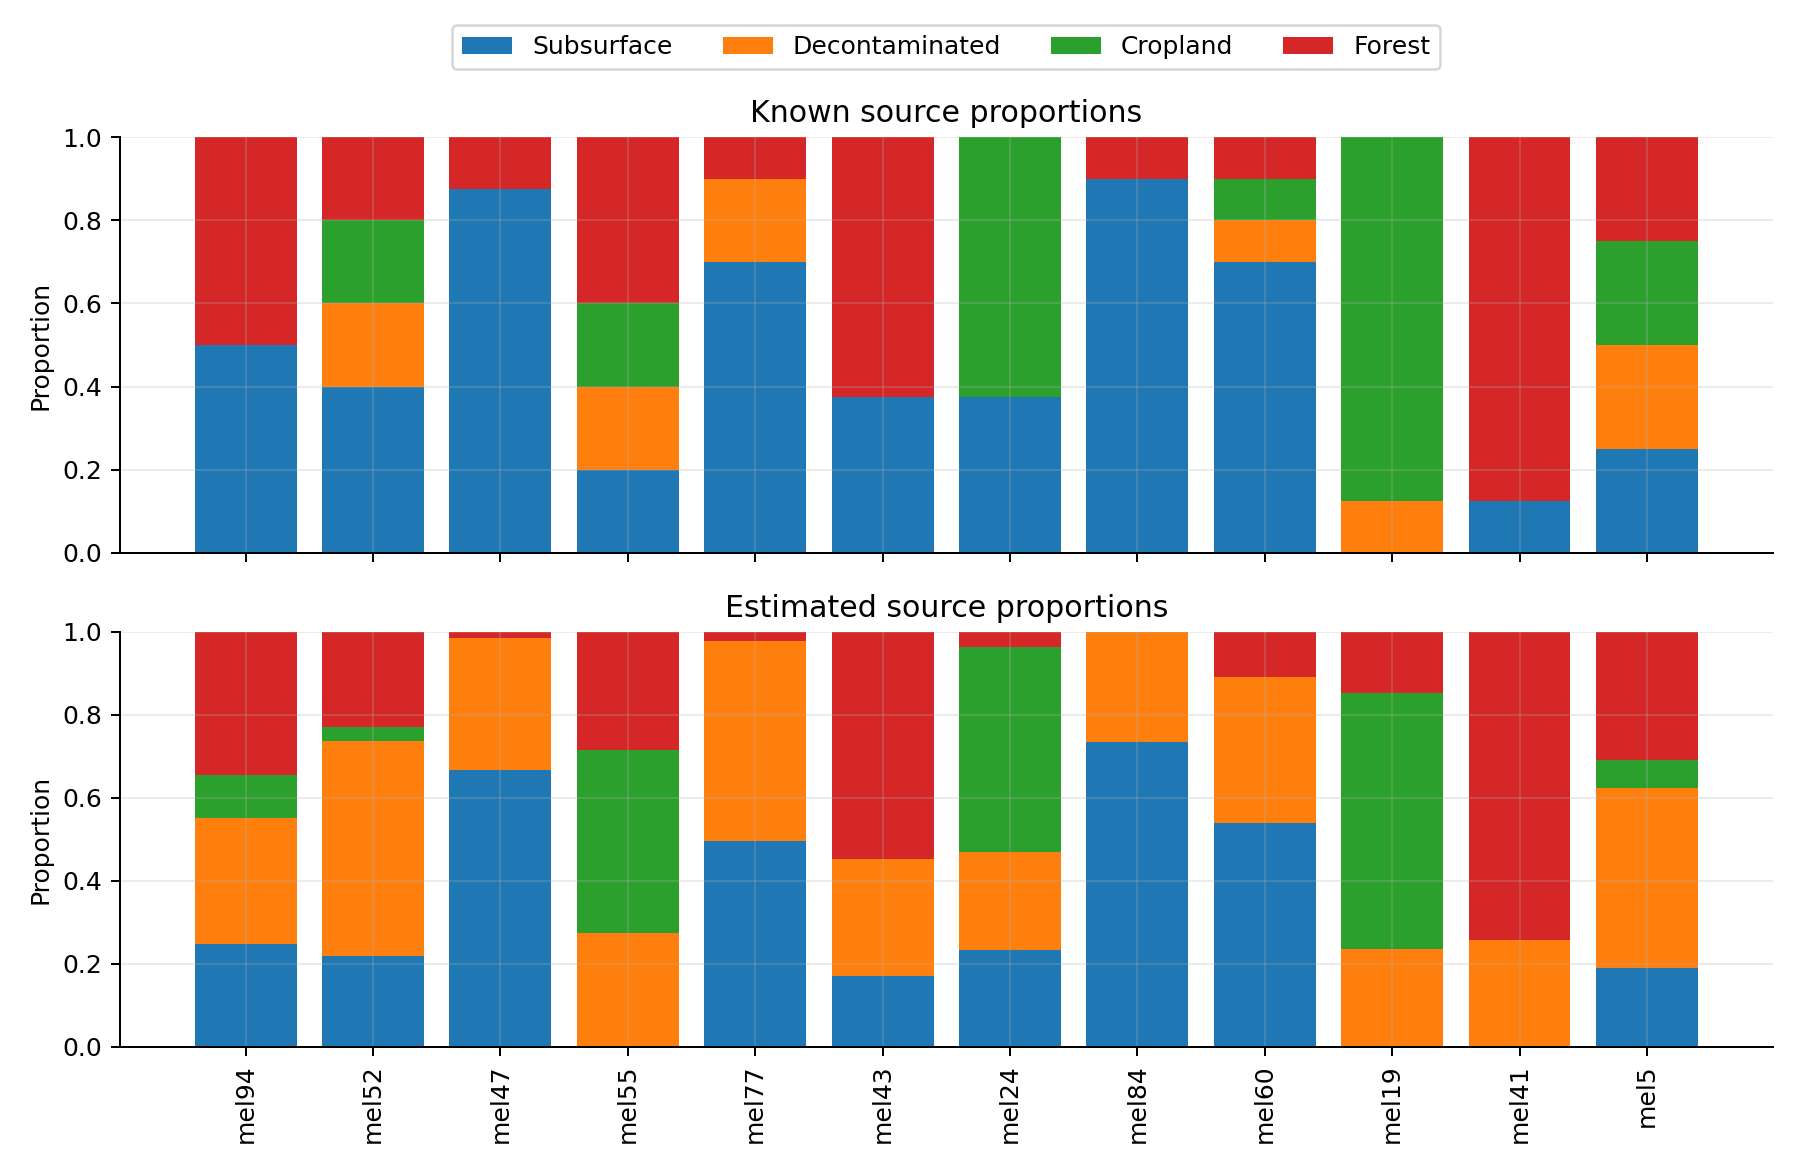
\includegraphics[keepaspectratio]{5-climate-and-environmental-systems/../notebooks-and-scripts/5-climate-and-environmental-systems/1-sediment-source-modeling/python/2-sediment-source-modeling-mccaffrey-figures/figures/mccaffrey_known_vs_estimated_representative_compositions.png}}

}

\caption{\label{fig-mccaffrey-representative-signatures}Known and
reconstructed representative source compositions obtained with the
McCaffrey constrained least-squares model.}

\end{figure}%

\subsubsection{Source Apportionment}\label{source-apportionment-1}

The constrained least-squares model was subsequently applied to every
laboratory mixture included in the benchmark dataset. The estimated
source proportions are compared with the known values in
Figure~\ref{fig-mccaffrey-estimated-vs-true}. Most predictions lie close
to the one-to-one reference line, suggesting that the deterministic
optimization captures the overall mixing behaviour despite the absence
of an explicit uncertainty model.

\begin{figure}

\centering{

\pandocbounded{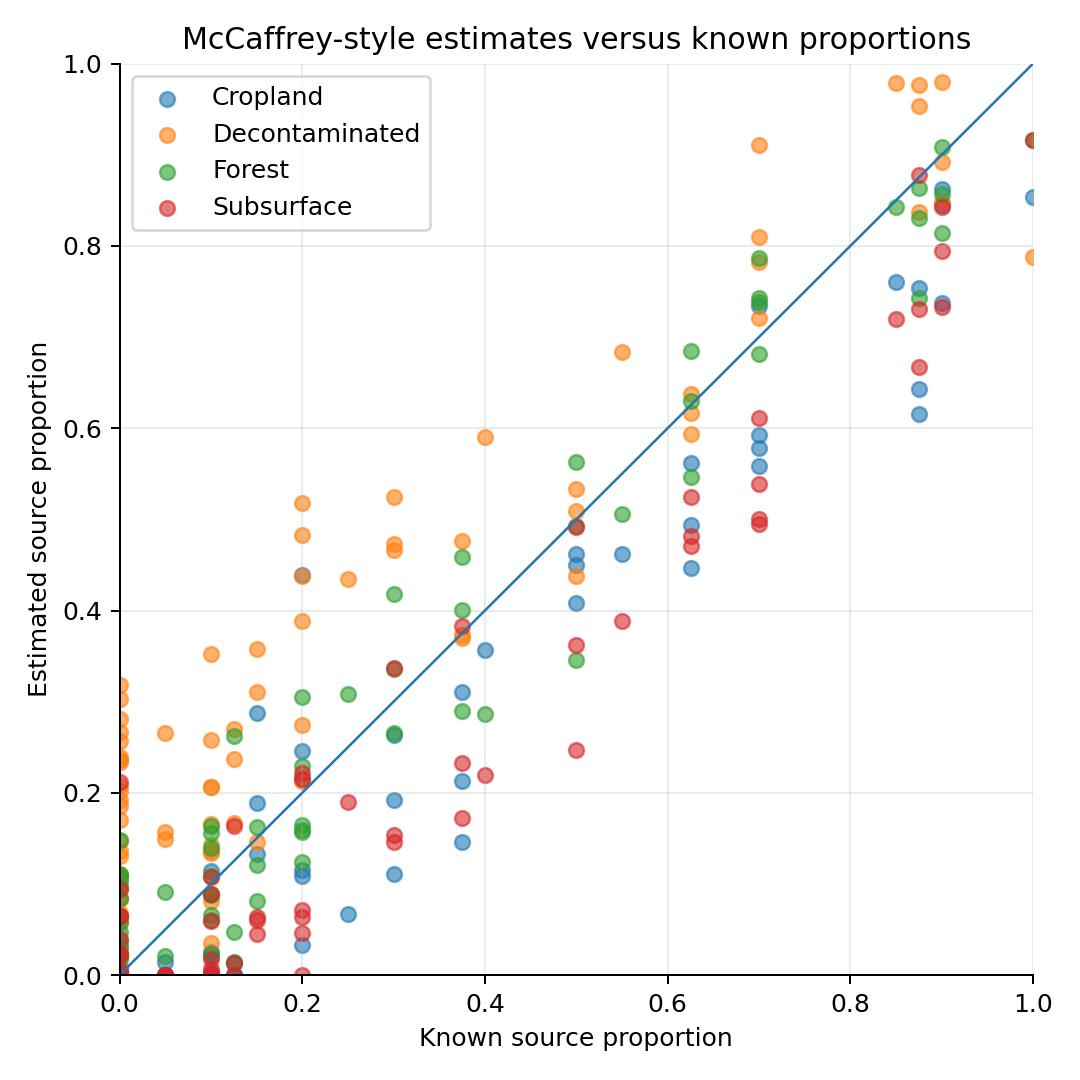
\includegraphics[keepaspectratio]{5-climate-and-environmental-systems/../notebooks-and-scripts/5-climate-and-environmental-systems/1-sediment-source-modeling/python/2-sediment-source-modeling-mccaffrey-figures/figures/mccaffrey_estimated_vs_true.png}}

}

\caption{\label{fig-mccaffrey-estimated-vs-true}Estimated versus true
source contributions obtained with the McCaffrey constrained
least-squares model.}

\end{figure}%

Overall performance is summarized in
Table~\ref{tbl-mccaffrey-performance}. The model achieves a mean
absolute error of approximately 0.08, an RMSE of 0.11, and a
Nash--Sutcliffe efficiency close to 0.87. In addition, the dominant
sediment source is correctly identified for more than 83\% of the
evaluated mixtures, demonstrating that the deterministic formulation
preserves most of the information required for practical source
attribution.

\begin{longtable}[]{@{}cc@{}}
\caption{Overall performance of the McCaffrey constrained least-squares
model.}\label{tbl-mccaffrey-performance}\tabularnewline
\toprule\noalign{}
\textbf{Metric} & \textbf{Value} \\
\midrule\noalign{}
\endfirsthead
\toprule\noalign{}
\textbf{Metric} & \textbf{Value} \\
\midrule\noalign{}
\endhead
\bottomrule\noalign{}
\endlastfoot
Mean Absolute Error (MAE) & 0.0793 \\
Root Mean Squared Error (RMSE) & 0.1086 \\
Nash--Sutcliffe Efficiency (NSE) & 0.8683 \\
Dominant Source Accuracy & 0.8354 \\
Mean Aitchison Distance & 16.6797 \\
\end{longtable}

The aggregated metrics conceal some differences between sediment
sources. As shown in Table~\ref{tbl-mccaffrey-source-metrics}, Forest
and Cropland exhibit the smallest prediction errors, whereas the
Decontaminated source shows the largest bias. This behaviour is
consistent with the greater overlap between some geochemical
fingerprints observed during the exploratory analysis.

\begin{longtable}[]{@{}cccc@{}}
\caption{Source-level performance metrics for the McCaffrey constrained
least-squares model.}\label{tbl-mccaffrey-source-metrics}\tabularnewline
\toprule\noalign{}
\textbf{Source} & \textbf{MAE} & \textbf{RMSE} & \textbf{Mean Error} \\
\midrule\noalign{}
\endfirsthead
\toprule\noalign{}
\textbf{Source} & \textbf{MAE} & \textbf{RMSE} & \textbf{Mean Error} \\
\midrule\noalign{}
\endhead
\bottomrule\noalign{}
\endlastfoot
Subsurface & 0.0768 & 0.1037 & -0.0601 \\
Decontaminated & 0.1234 & 0.1517 & 0.1106 \\
Cropland & 0.0693 & 0.0975 & -0.0532 \\
Forest & 0.0478 & 0.0625 & 0.0028 \\
\end{longtable}

Compared with the probabilistic BMM, the McCaffrey model sacrifices
uncertainty quantification in exchange for a considerably simpler
optimization procedure and a single deterministic estimate for each
mixture. This trade-off does not necessarily represent a limitation; in
many industrial applications, a stable point estimate is preferable when
uncertainty intervals are not required for operational decision-making.

\subsection{Sandoval Ratio-Based Mixing
Model}\label{sandoval-ratio-based-mixing-model}

The final approach implements the ratio-based constrained deconvolution
model proposed by Sandoval et al.
\citeproc{ref-sandoval2022original}{{[}32{]}}. Although it addresses the
same source apportionment problem as the McCaffrey model, it adopts a
different representation of the geochemical data. Instead of comparing
elemental concentrations directly, the optimization is performed using
log-ratios between tracers, reducing the influence of the constant-sum
constraint that characterizes compositional datasets.

This formulation is particularly attractive for geochemical applications
because many analytical measurements are inherently relative rather than
absolute. By expressing the observations as ratios, the optimization
focuses on the proportional relationships between tracers instead of
their individual magnitudes, making the solution less sensitive to
scaling effects and compositional closure.

A complete Python implementation of the Sandoval ratio-based mixing
model presented in this section is available in the project repository
\href{https://github.com/rodrigokang/portfolio/tree/main/notebooks-and-scripts/5-climate-and-environmental-systems/1-sediment-source-modeling}{here}.

\subsubsection{Representative Source
Signatures}\label{representative-source-signatures-1}

As in the McCaffrey formulation, a representative fingerprint was first
constructed for each sediment source. These reference signatures were
subsequently transformed into a log-ratio representation before solving
the constrained optimization problem.

The tracer-specific scaling factors used during preprocessing are
summarized in Table~\ref{tbl-sandoval-scaling-factors}.

\begin{longtable}[]{@{}cc@{}}
\caption{Scaling factors applied to the selected geochemical tracers
prior to log-ratio
transformation.}\label{tbl-sandoval-scaling-factors}\tabularnewline
\toprule\noalign{}
\textbf{Tracer} & \textbf{Scaling Factor} \\
\midrule\noalign{}
\endfirsthead
\toprule\noalign{}
\textbf{Tracer} & \textbf{Scaling Factor} \\
\midrule\noalign{}
\endhead
\bottomrule\noalign{}
\endlastfoot
L & 51.728 \\
h & 74.501 \\
Si & 214014.572 \\
Zn & 135.606 \\
Mn & 972.318 \\
Ti & 4696.537 \\
K & 2784.897 \\
C* & 3.657 \\
Y & 5.830 \\
\end{longtable}

The reconstructed representative compositions are compared with the
observed source fingerprints in
Figure~\ref{fig-sandoval-representative-signatures}. Despite operating
in log-ratio space, the model accurately reproduces the characteristic
geochemical signatures of the four sediment sources, indicating that the
transformation preserves the relevant compositional information.

\begin{figure}

\centering{

\pandocbounded{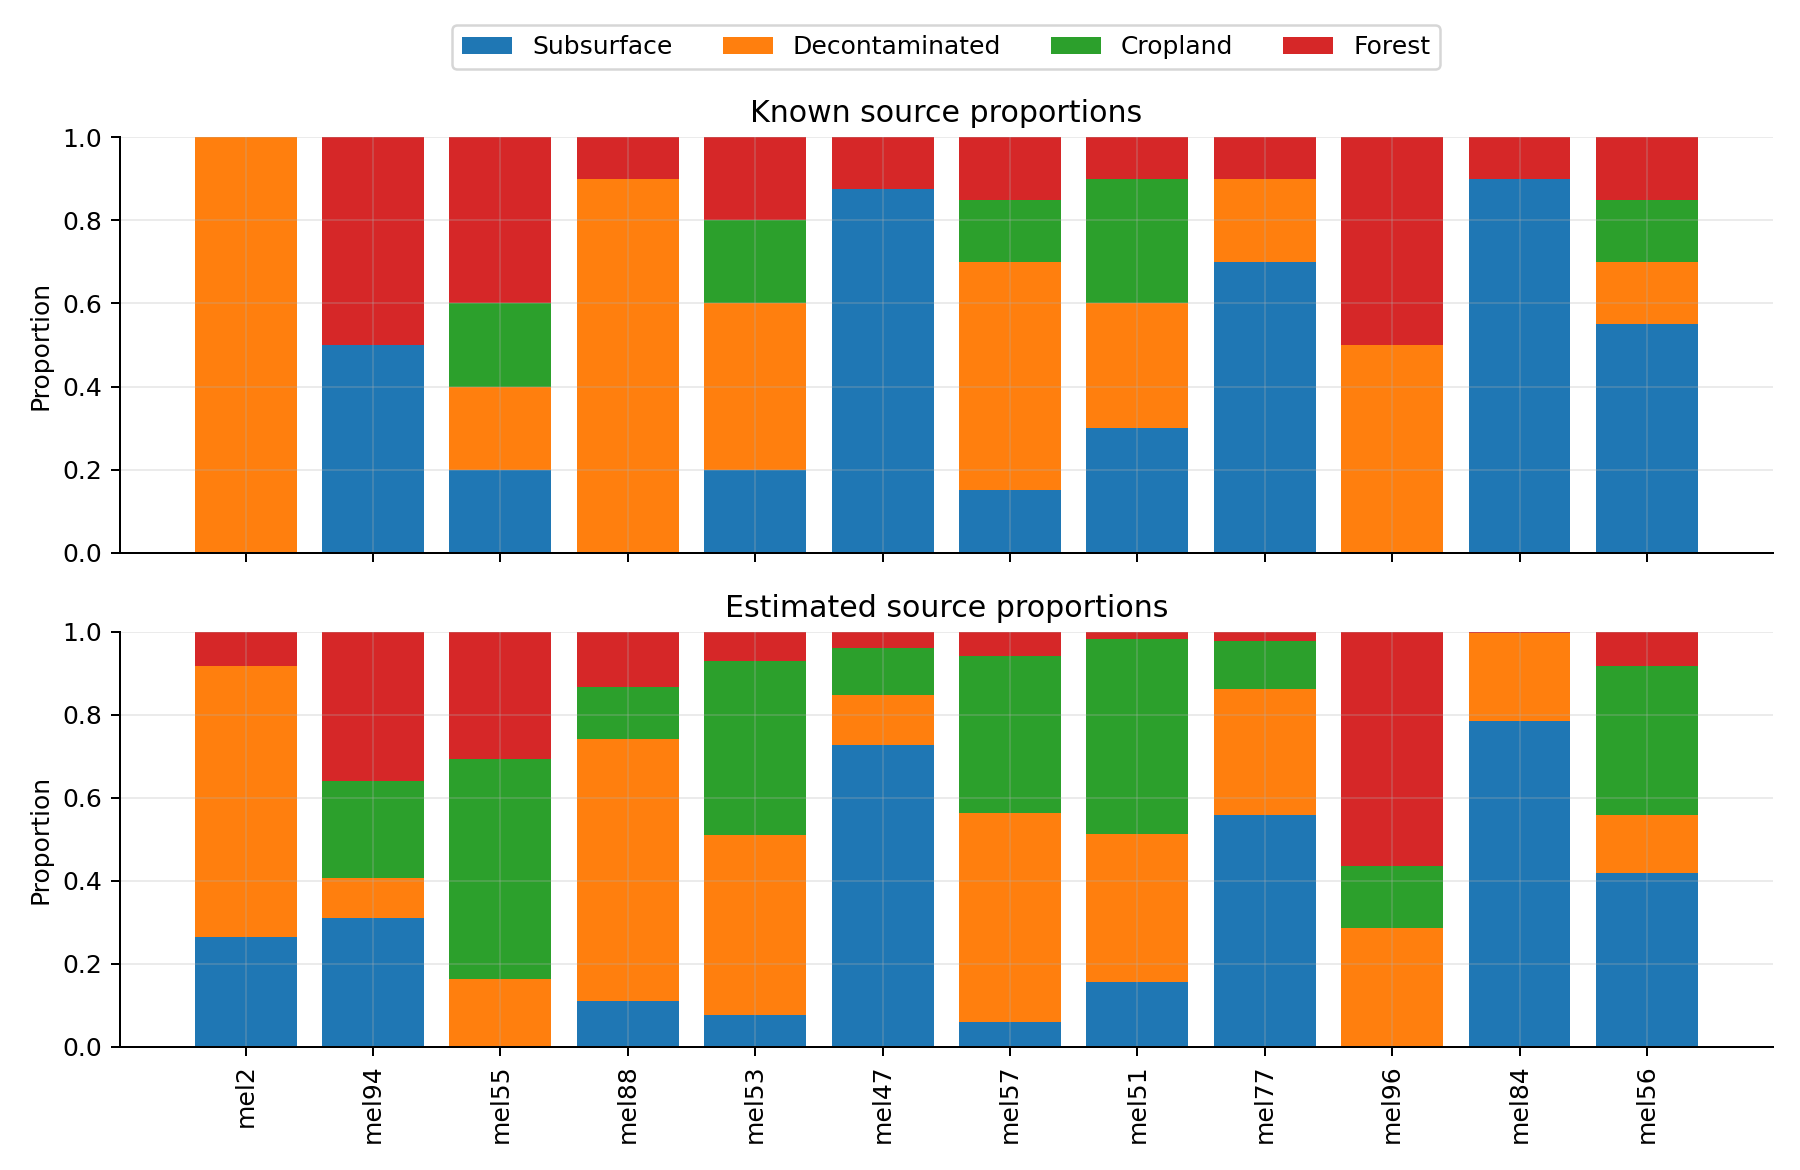
\includegraphics[keepaspectratio]{5-climate-and-environmental-systems/../notebooks-and-scripts/5-climate-and-environmental-systems/1-sediment-source-modeling/python/3-sediment-source-modeling-sandoval-figures/figures/sandoval_known_vs_estimated_representative_compositions.png}}

}

\caption{\label{fig-sandoval-representative-signatures}Known and
reconstructed representative source compositions obtained with the
Sandoval ratio-based model.}

\end{figure}%

\subsubsection{Source Apportionment}\label{source-apportionment-2}

After calibration, the ratio-based model was applied to the laboratory
mixtures using the same benchmark dataset employed for the previous
methods. The estimated source proportions are compared with the known
values in Figure~\ref{fig-sandoval-estimated-vs-true}. Most predictions
remain close to the one-to-one reference line, indicating that the
log-ratio formulation successfully recovers the dominant source
proportions while maintaining numerical stability throughout the
optimization.

\begin{figure}

\centering{

\pandocbounded{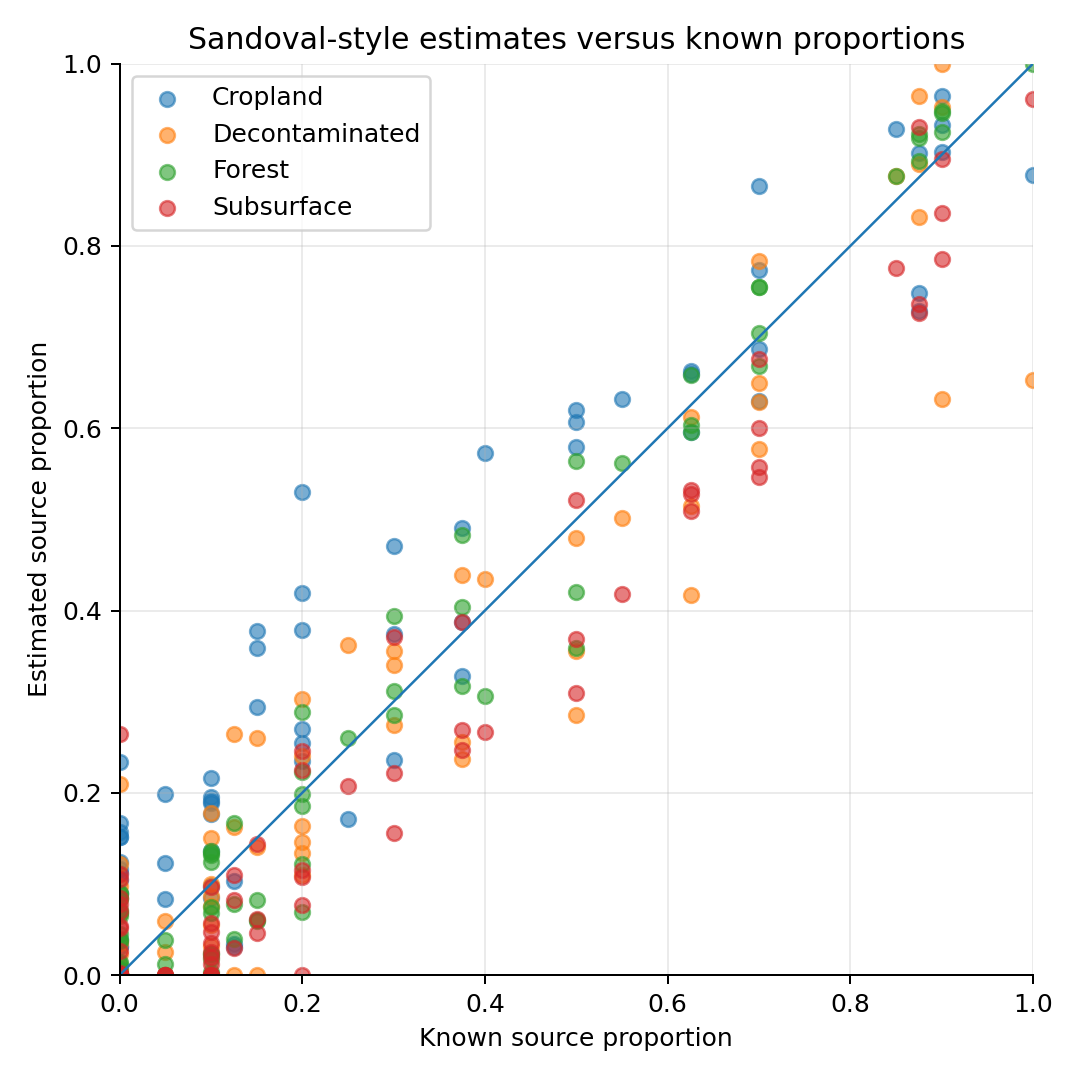
\includegraphics[keepaspectratio]{5-climate-and-environmental-systems/../notebooks-and-scripts/5-climate-and-environmental-systems/1-sediment-source-modeling/python/3-sediment-source-modeling-sandoval-figures/figures/sandoval_estimated_vs_true.png}}

}

\caption{\label{fig-sandoval-estimated-vs-true}Estimated versus true
source contributions obtained with the Sandoval ratio-based model.}

\end{figure}%

The overall performance metrics are summarized in
Table~\ref{tbl-sandoval-performance}. Compared with the McCaffrey
formulation, the ratio-based model achieves lower prediction errors, a
higher Nash--Sutcliffe efficiency, and a modest improvement in dominant
source identification. The average Aitchison distance also decreases,
suggesting that representing the mixtures in log-ratio space provides a
more appropriate description of compositional differences.

\begin{longtable}[]{@{}cc@{}}
\caption{Overall performance of the Sandoval ratio-based mixing
model.}\label{tbl-sandoval-performance}\tabularnewline
\toprule\noalign{}
\textbf{Metric} & \textbf{Value} \\
\midrule\noalign{}
\endfirsthead
\toprule\noalign{}
\textbf{Metric} & \textbf{Value} \\
\midrule\noalign{}
\endhead
\bottomrule\noalign{}
\endlastfoot
Mean Absolute Error (MAE) & 0.0620 \\
Root Mean Squared Error (RMSE) & 0.0864 \\
Nash--Sutcliffe Efficiency (NSE) & 0.9166 \\
Dominant Source Accuracy & 0.8481 \\
Mean Aitchison Distance & 14.3363 \\
Mean Ratio Objective & 0.00143 \\
\end{longtable}

The source-level results presented in
Table~\ref{tbl-sandoval-source-metrics} provide a more detailed
perspective on model performance. Forest exhibits the smallest
reconstruction error, whereas Cropland remains the most challenging
source to estimate accurately, consistent with the overlap observed
during the exploratory analysis.

\begin{longtable}[]{@{}cccc@{}}
\caption{Source-level performance metrics for the Sandoval ratio-based
mixing model.}\label{tbl-sandoval-source-metrics}\tabularnewline
\toprule\noalign{}
\textbf{Source} & \textbf{MAE} & \textbf{RMSE} & \textbf{Mean Error} \\
\midrule\noalign{}
\endfirsthead
\toprule\noalign{}
\textbf{Source} & \textbf{MAE} & \textbf{RMSE} & \textbf{Mean Error} \\
\midrule\noalign{}
\endhead
\bottomrule\noalign{}
\endlastfoot
Subsurface & 0.0656 & 0.0866 & -0.0384 \\
Decontaminated & 0.0609 & 0.0909 & -0.0151 \\
Cropland & 0.0799 & 0.1055 & 0.0515 \\
Forest & 0.0415 & 0.0545 & 0.0019 \\
\end{longtable}

One practical advantage of the Sandoval formulation is that it naturally
accommodates the relative nature of geochemical measurements without
increasing the complexity of the optimization procedure. While both
deterministic approaches produce comparable source apportionments, the
log-ratio representation provides a measurable improvement in
reconstruction accuracy and compositional consistency, making it the
strongest deterministic performer among the three methods evaluated in
this study.

\section{Results, Discussion, and
Limitations}\label{results-discussion-and-limitations-10}

Although the three source apportionment methods were developed from
different modelling philosophies, all successfully recovered the source
proportions of the benchmark mixtures. This agreement is perhaps the
most important outcome of the study. Rather than demonstrating the
superiority of a particular algorithm, it shows that the underlying
inverse problem is sufficiently well posed to admit multiple valid
formulations. Whether approached through probabilistic resampling,
constrained least-squares optimization, or log-ratio deconvolution, the
essential objective remains the same: identifying the combination of
source proportions that best explains the measured geochemical
composition while satisfying the physical constraints of the mixing
process.

The Bootstrapped Mixing Model provides the richest representation of the
problem by explicitly accounting for uncertainty. Instead of producing a
single estimate, it generates confidence intervals that reflect both
analytical variability and the natural overlap between source
fingerprints. This additional information is particularly valuable when
the estimated proportions are intended to support environmental
interpretation, where understanding the confidence associated with a
prediction is often as important as the prediction itself. The price for
this richer representation is a more computationally intensive workflow
that requires repeated resampling and optimization.

The deterministic formulations approach the problem from a different
perspective. By directly solving a constrained optimization problem,
they produce a single physically consistent estimate for each sediment
mixture without explicitly modelling uncertainty. This considerably
simplifies the computational workflow while preserving the physical
constraints that define a valid compositional mixture.

Between the two deterministic approaches, the ratio-based formulation
proposed by Sandoval et al.~consistently achieved the strongest overall
performance. Although both methods rely on the same optimization
principles, representing the observations in log-ratio space reduces the
influence of compositional closure and places greater emphasis on the
relative relationships between tracers. The resulting improvements in
reconstruction accuracy are modest but consistent across the evaluation
metrics, suggesting that explicitly accounting for the compositional
nature of the data provides a measurable practical advantage.

Perhaps the most interesting outcome of the comparison lies beyond the
numerical results themselves. The two deterministic methods were
originally developed for petroleum production allocation, yet they
required remarkably few conceptual modifications before being applied to
sediment fingerprinting. The optimization problem, the governing
constraints, and the mathematical formulation remain essentially
unchanged; only the interpretation of the sources differs. Reservoirs
contributing to a commingled production stream become sediment-producing
landscape units, while reservoir geochemical fingerprints become
sediment fingerprints. This demonstrates that many inverse problems
share a common mathematical structure despite arising in entirely
different scientific domains.

Several limitations should nevertheless be acknowledged. The evaluation
is based on laboratory-prepared mixtures and synthetically generated
benchmark datasets, where the true source proportions are known exactly.
While these datasets provide an objective basis for comparing competing
methods, natural catchments often exhibit greater spatial variability,
temporal changes in source composition, and additional measurement
uncertainty that cannot be fully reproduced under controlled
experimental conditions. Furthermore, all three methods assume that the
selected tracers behave conservatively during erosion, transport, and
deposition. Processes that preferentially alter or fractionate
individual tracers could violate this assumption and reduce the
reliability of the estimated proportions.

Overall, the results indicate that no single method is universally
preferable. The Bootstrapped Mixing Model is the natural choice when
uncertainty quantification is an essential component of the analysis,
whereas the deterministic formulations provide simpler and
computationally efficient alternatives when a single robust estimate is
sufficient. Among these, the ratio-based model offers the best balance
between numerical stability and predictive accuracy.

Beyond the comparison itself, this project illustrates a broader
principle that appears repeatedly throughout this portfolio. Effective
data science is often less about developing entirely new algorithms than
about recognizing when an existing mathematical formulation can be
transferred to a different domain. Once the underlying structure of a
problem has been identified, methodologies developed for one application
can often provide effective solutions to another with only minor
adaptations. In this study, techniques originally designed for petroleum
production allocation proved equally capable of solving a sediment
source apportionment problem, highlighting the value of focusing on
mathematical structure rather than disciplinary boundaries.

\section{Technical Appendix
(Optional)}\label{technical-appendix-optional-9}

The three source apportionment methods presented in this chapter
originate from different scientific disciplines and employ different
estimation strategies. Nevertheless, they all solve the same underlying
inverse problem: recovering the relative proportions of multiple sources
whose combined geochemical signatures reproduce an observed sediment
mixture.

Recognizing this common mathematical structure is often more valuable
than studying each algorithm in isolation. Once the inverse mixing
problem has been defined, the differences between the Bootstrapped
Mixing Model, the McCaffrey formulation, and the Sandoval formulation
reduce primarily to how the solution is estimated and how uncertainty is
represented.

Rather than reviewing the implementation details presented earlier in
the chapter, this appendix focuses on the mathematical concepts shared
by all three approaches before introducing the ideas that distinguish
them. The discussion begins with the linear mixing model, proceeds to
the inverse problem and its physical constraints, and then examines how
probabilistic and deterministic formulations provide alternative
solutions to the same estimation problem.

The conceptual relationships among these ideas are summarized in
Figure~\ref{fig-source-apportionment-framework}. Although the three
methods differ in how they estimate the unknown source proportions, they
all originate from the same physical mixing model, share the same
constrained inverse formulation, and differ primarily in how uncertainty
is represented and how the objective function is defined.

\begin{figure}

\centering{

\pandocbounded{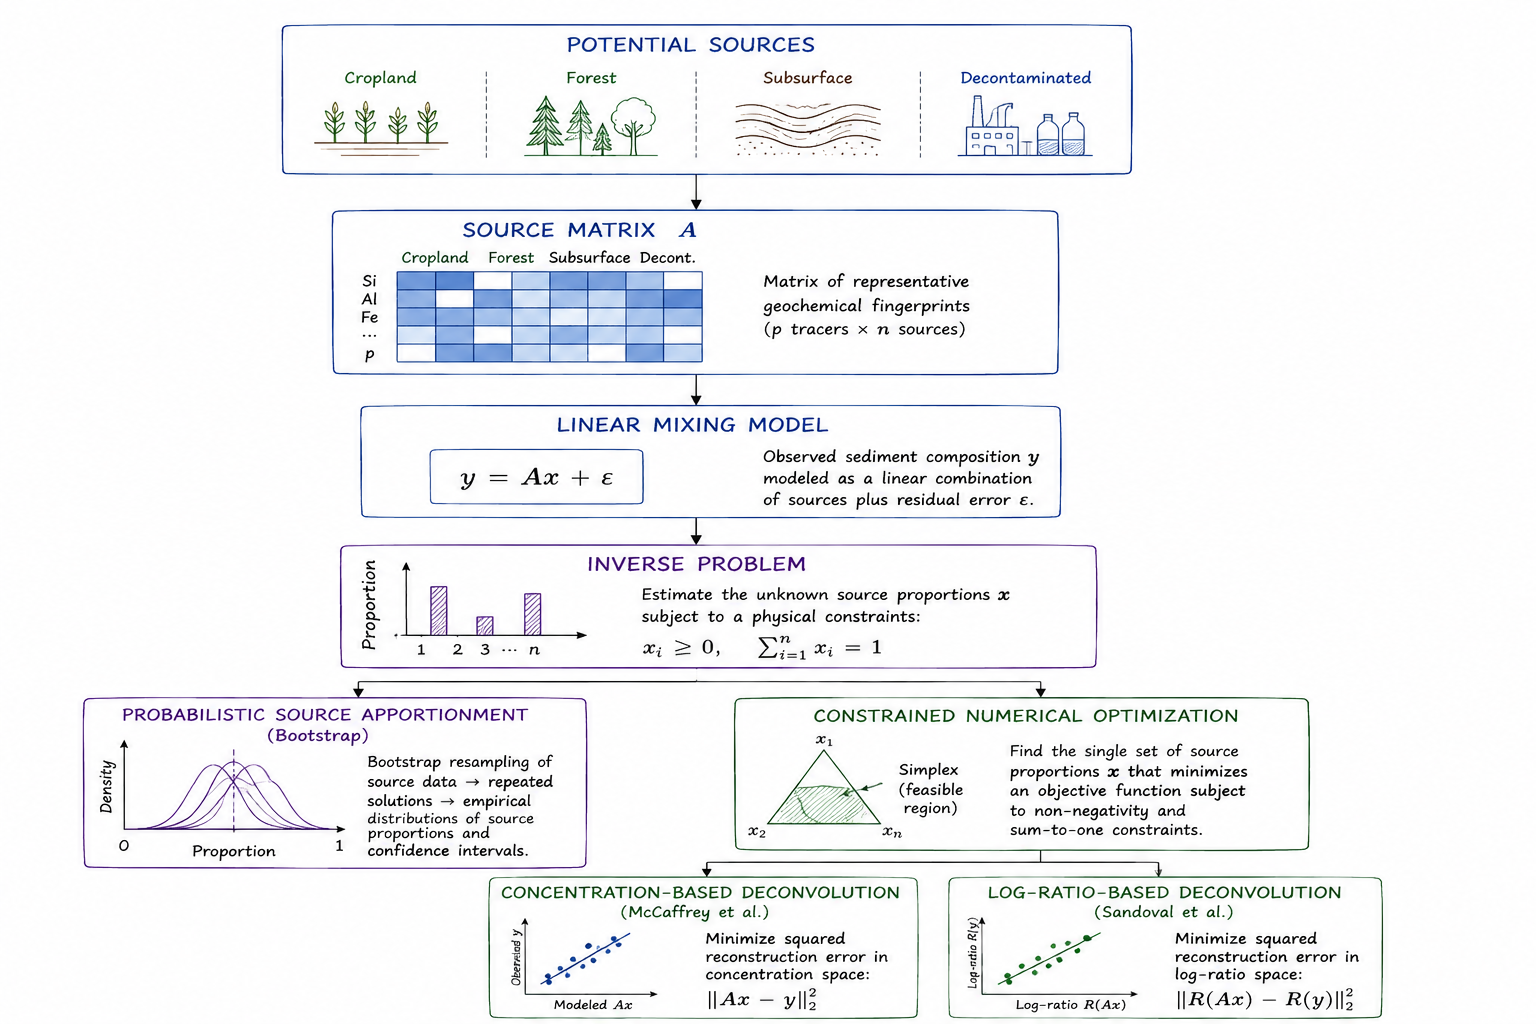
\includegraphics[keepaspectratio]{5-climate-and-environmental-systems/figures/conceptual-framework-source-apportionment.png}}

}

\caption{\label{fig-source-apportionment-framework}Conceptual framework
of the source apportionment problem. All three methods considered in
this chapter solve the same inverse mixing problem under identical
physical constraints, differing only in how uncertainty is represented
and how the objective function is formulated.}

\end{figure}%

\subsection{Linear Mixing Models}\label{linear-mixing-models}

At the core of sediment fingerprinting lies a simple physical
assumption: the geochemical composition measured in a sediment sample
results from mixing material originating from several upstream sources.
If the selected tracers behave conservatively---that is, they are
neither created nor destroyed during erosion, transport, and
deposition---the composition of the mixture can be approximated as a
weighted combination of the compositions of its constituent sources.

This assumption is known as the \textbf{linear mixing model} and forms
the mathematical foundation of every source apportionment method
presented in this chapter. Although the three approaches differ in how
they estimate the unknown source proportions, they all rely on the same
physical description of the mixing process.

Suppose that \(m\) geochemical tracers are measured for \(n\) potential
sediment sources. The corresponding source fingerprints can then be
arranged into the matrix

\begin{equation}\phantomsection\label{eq-source-matrix}{
\mathbf{A} =
\begin{bmatrix}
a_{11} & a_{12} & \cdots & a_{1n} \\
a_{21} & a_{22} & \cdots & a_{2n} \\
\vdots & \vdots & \ddots & \vdots \\
a_{m1} & a_{m2} & \cdots & a_{mn}
\end{bmatrix},
}\end{equation}

where each column corresponds to one sediment source and each row
contains the concentration of a particular tracer measured for that
source.

The observed sediment mixture is represented by

\begin{equation}\phantomsection\label{eq-mixture-vector}{
\mathbf{y} =
\begin{bmatrix}
y_1 \\
y_2 \\
\vdots \\
y_m
\end{bmatrix},
}\end{equation}

while the unknown source proportions are collected in

\begin{equation}\phantomsection\label{eq-source-proportions}{
\mathbf{x} =
\begin{bmatrix}
x_1 \\
x_2 \\
\vdots \\
x_n
\end{bmatrix},
}\end{equation}

where each component represents the fraction of sediment contributed by
one source.

Under the assumption of conservative mixing, the relationship between
the source fingerprints and the measured sediment composition is
expressed as

\begin{equation}\phantomsection\label{eq-linear-mixing-model}{
\mathbf{y}=\mathbf{A}\mathbf{x}+\boldsymbol{\varepsilon},
}\end{equation}

where \(\boldsymbol{\varepsilon}\) represents measurement uncertainty
together with any discrepancy between the simplified mixing model and
the observations.

Although deceptively compact, Equation~\ref{eq-linear-mixing-model}
encapsulates the entire source apportionment problem. The matrix
\(\mathbf{A}\) is assumed to be known from measurements collected at the
potential source areas, while the mixture vector \(\mathbf{y}\) is
obtained from downstream samples. The only unknown quantity is the
vector of source proportions \(\mathbf{x}\), which becomes the target of
the estimation process.

The challenge, however, is that estimating \(\mathbf{x}\) is
considerably more difficult than evaluating
Equation~\ref{eq-linear-mixing-model} in the forward direction.
Recovering the source proportions from an observed mixture requires
solving an inverse problem, where multiple solutions may reproduce the
measured composition with similar accuracy.

\subsection{The Inverse Mixing
Problem}\label{the-inverse-mixing-problem}

If the source proportions are known, predicting the composition of the
resulting sediment mixture is straightforward: the linear mixing model
introduced in Equation~\ref{eq-linear-mixing-model} can be evaluated
directly by multiplying the source matrix by the vector of source
proportions. This is commonly referred to as the \textbf{forward
problem}.

Sediment source apportionment, however, requires solving the opposite
task. The measured sediment composition is available, but the
proportions contributed by each source are unknown. The objective is
therefore to estimate the vector \(\mathbf{x}\) from the mixture vector
\(\mathbf{y}\) and the known source fingerprints contained in
\(\mathbf{A}\). This inverse formulation is considerably more
challenging because the solution cannot generally be obtained by simply
rearranging Equation~\ref{eq-linear-mixing-model}.

Several factors contribute to this difficulty. First, laboratory
measurements inevitably contain analytical uncertainty, meaning that the
measured composition is only an approximation of the true mixture.
Second, different sediment sources often exhibit similar geochemical
fingerprints, making it difficult to distinguish their individual
contributions. Finally, environmental datasets typically contain only a
limited number of informative tracers, reducing the amount of
independent information available for estimating the unknown source
proportions.

These factors imply that multiple combinations of source proportions may
reproduce the measured composition with nearly identical accuracy.
Consequently, source apportionment should not be viewed as the search
for a unique exact solution, but rather as the identification of the
most plausible solution that remains consistent with both the
observations and the underlying physics of the mixing process.

Physical considerations impose two additional constraints on every
admissible solution. Because the unknown variables represent
proportions, they cannot be negative,

\begin{equation}\phantomsection\label{eq-nonnegative}{
x_i \ge 0,
\qquad i=1,\ldots,n,
}\end{equation}

and, because the entire sediment sample must originate from the
available sources, the proportions must sum to one,

\begin{equation}\phantomsection\label{eq-sum-one}{
\sum_{i=1}^{n} x_i = 1.
}\end{equation}

These constraints are not merely mathematical conveniences; they reflect
the conservation of mass and ensure that every estimated source
apportionment has a physically meaningful interpretation. Any solution
violating either condition would imply either negative sediment
contributions or the artificial creation (or loss) of material during
the mixing process.

Together, Equation~\ref{eq-nonnegative} and Equation~\ref{eq-sum-one}
define the feasible solution space explored by all three methods
presented in this chapter. The principal difference between the
Bootstrapped Mixing Model, the McCaffrey formulation, and the Sandoval
formulation lies not in these physical constraints, which are common to
all approaches, but in how each method explores this feasible space and
identifies the solution that best explains the measured composition.

\subsection{Constrained Numerical
Optimization}\label{constrained-numerical-optimization}

Once the inverse mixing problem has been formulated, the next question
is how the unknown source proportions should be estimated. In principle,
one might attempt to solve Equation~\ref{eq-linear-mixing-model}
analytically using ordinary least squares. Such an approach minimizes
the discrepancy between the measured composition and the reconstructed
mixture, producing the solution that best fits the available
observations in a purely algebraic sense.

In practice, however, unconstrained least-squares solutions are not
guaranteed to satisfy the physical requirements established in
Equation~\ref{eq-nonnegative} and Equation~\ref{eq-sum-one}. Small
measurement errors, correlated tracers, or poorly conditioned source
matrices may produce negative proportions or values exceeding one.
Although these solutions minimize the residual error, they cannot
represent physically meaningful sediment mixtures.

For this reason, the deterministic methods implemented in this project
were reformulated as constrained numerical optimization problems. Rather
than solving the system analytically and verifying the constraints
afterwards, the optimization searches directly within the physically
admissible solution space. Every candidate solution therefore satisfies
the non-negativity and mass conservation constraints throughout the
optimization process.

The general optimization problem can be written as

\begin{equation}\phantomsection\label{eq-constrained-optimization}{
\begin{aligned}
\min_{\mathbf{x}}\quad & f(\mathbf{x}) \\
\text{subject to}\quad
& x_i \ge 0,\qquad i=1,\ldots,n,\\
& \sum_{i=1}^{n}x_i = 1,
\end{aligned}
}\end{equation}

where the objective function \(f(\mathbf{x})\) depends on the particular
source apportionment method being used. The optimization variables are
always the unknown source proportions, while the physical constraints
remain unchanged.

Reformulating the estimation in this way offers several practical
advantages. First, every solution returned by the optimizer is
physically interpretable, eliminating the need for post-processing
corrections to enforce valid proportions. Second, the optimization
framework is independent of the specific objective function. This makes
it possible to compare different source apportionment formulations while
using exactly the same numerical solution strategy.

This separation between the optimization algorithm and the objective
function is one of the central design principles of the implementation
developed for this project. The McCaffrey and Sandoval methods differ
primarily in the quantity they seek to minimize, yet both can be solved
using the same constrained optimization framework introduced in
Equation~\ref{eq-constrained-optimization}. As a result, differences in
performance can be attributed to the modelling formulation itself rather
than to changes in the numerical solution procedure.

The Bootstrapped Mixing Model follows a different estimation strategy.
Instead of searching for a single optimal solution, it repeatedly
perturbs the source fingerprints through bootstrap resampling and solves
the mixing problem many times. Nevertheless, each realization remains
subject to the same physical constraints, ensuring that every sampled
source apportionment represents a feasible sediment mixture. The
principal distinction between the probabilistic and deterministic
approaches therefore lies not in the underlying physics, but in how
uncertainty is represented and propagated through the estimation
process.

\subsection{Probabilistic Source
Apportionment}\label{probabilistic-source-apportionment}

The deterministic optimization framework described in the previous
section assumes that the source fingerprints are known exactly. In
practice, however, geochemical measurements are subject to analytical
uncertainty, natural spatial variability, and sampling error. As a
result, the representative fingerprint assigned to each sediment source
should be regarded as an estimate rather than as a fixed quantity.

The Bootstrapped Mixing Model (BMM) addresses this uncertainty by
repeatedly resampling the available source observations before solving
the mixing problem. Instead of producing a single estimate of the source
proportions, the model generates a large collection of equally plausible
solutions, each corresponding to a different realization of the source
fingerprints. The variability among these solutions provides a direct
estimate of the uncertainty associated with the predicted proportions.

The procedure can be summarized as four consecutive steps:

\begin{enumerate}
\def\labelenumi{\arabic{enumi}.}
\tightlist
\item
  A bootstrap sample is generated independently for each sediment source
  by randomly resampling the available geochemical observations with
  replacement.
\item
  Representative source fingerprints are computed from the resampled
  datasets.
\item
  The source apportionment problem is solved using the reconstructed
  fingerprints.
\item
  The process is repeated many times to obtain an empirical distribution
  of the estimated source proportions.
\end{enumerate}

Because each bootstrap realization is treated as an equally plausible
representation of the original dataset, the collection of estimated
source proportions approximates the sampling distribution of the unknown
solution. Confidence intervals can then be obtained directly from the
empirical quantiles without requiring any assumption about the
analytical form of the underlying probability distribution.

Conceptually, the procedure can be written as

\begin{equation}\phantomsection\label{eq-bootstrap-optimization}{
\mathbf{x}^{(b)}
=
\operatorname*{arg\,min}_{\mathbf{x}}
f_b(\mathbf{x}),
\qquad
b=1,\ldots,B,
}\end{equation}

where \(B\) denotes the number of bootstrap realizations and
\(f_b(\mathbf{x})\) is the objective function associated with the
\(b\)-th resampled dataset. Each optimization is solved independently,
producing a collection of estimated source proportions,

\begin{equation}\phantomsection\label{eq-bootstrap-samples}{
\left\{
\mathbf{x}^{(1)},
\mathbf{x}^{(2)},
\ldots,
\mathbf{x}^{(B)}
\right\},
}\end{equation}

from which summary statistics such as the mean, median, prediction
intervals, and confidence intervals can be computed.

An important consequence of this formulation is that uncertainty arises
naturally from the variability of the source fingerprints rather than
being imposed through an explicit probabilistic model. The bootstrap
therefore provides a practical way to propagate measurement uncertainty
through the source apportionment process while preserving the physical
constraints introduced in Equation~\ref{eq-constrained-optimization} for
every realization.

Unlike the deterministic methods discussed later in this appendix, the
objective of the Bootstrapped Mixing Model is not to identify a single
optimal solution. Instead, it characterizes the range of solutions that
remain compatible with the observations. This distinction explains why
the BMM produces confidence intervals for the estimated source
proportions, whereas the deterministic formulations return only a single
point estimate for each sediment source.

\subsection{Concentration-Based
Deconvolution}\label{concentration-based-deconvolution}

The Bootstrapped Mixing Model characterizes uncertainty by repeatedly
perturbing the source fingerprints and solving the inverse problem many
times. The deterministic approaches follow a different philosophy.
Rather than estimating a distribution of plausible solutions, they seek
a single set of source proportions that best reproduces the measured
composition.

The first deterministic formulation considered in this chapter is based
on the constrained least-squares approach proposed by McCaffrey et al.
\citeproc{ref-mccaffrey2011geochemical}{{[}31{]}}. Originally developed
for geochemical allocation of commingled oil and gas production, the
method assumes that the measured composition of a mixture can be
reconstructed by combining the representative fingerprints of the
contributing sources.

Within the optimization framework introduced in
Equation~\ref{eq-constrained-optimization}, the McCaffrey formulation
defines the objective function as the squared Euclidean distance between
the measured composition and the composition reconstructed from the
estimated source proportions,

\begin{equation}\phantomsection\label{eq-mccaffrey-objective}{
f(\mathbf{x})
=
\left\|
\mathbf{A}\mathbf{x}
-
\mathbf{y}
\right\|_2^2.
}\end{equation}

The optimization therefore seeks the physically admissible source
proportions that minimize the overall reconstruction error while
satisfying the non-negativity and mass conservation constraints.

The least-squares criterion has an intuitive interpretation. If the
estimated source proportions perfectly reproduce the measured
composition, every residual becomes zero and the objective function
reaches its minimum possible value. In practice, measurement uncertainty
and natural variability prevent an exact reconstruction, so the
optimization instead identifies the solution with the smallest overall
discrepancy.

An important characteristic of this formulation is that all tracers
contribute simultaneously to the objective function. Rather than
attempting to match each geochemical variable independently, the
optimization balances the residuals across the complete fingerprint,
producing the set of source proportions that provides the best overall
agreement with the observations.

The constrained optimization framework adopted in this project differs
slightly from the original analytical formulation presented by McCaffrey
et al.~Instead of deriving the solution directly through matrix algebra,
the unknown source proportions are estimated numerically under the
physical constraints defined by Equation~\ref{eq-nonnegative} and
Equation~\ref{eq-sum-one}. Although both approaches solve the same
mathematical problem, the numerical formulation guarantees physically
admissible solutions while providing a common framework that can easily
be extended to alternative objective functions.

This flexibility becomes particularly valuable when the assumptions
underlying ordinary least squares are no longer appropriate. Geochemical
measurements are compositional by nature: only the relative
relationships between tracers are physically meaningful, while their
absolute magnitudes are affected by the constant-sum constraint. The
next section introduces the basic concepts of compositional data
analysis before presenting the log-ratio formulation proposed by
Sandoval et al., which explicitly accounts for these characteristics.

\subsection{Compositional Data
Analysis}\label{compositional-data-analysis}

The least-squares formulation presented in the previous section
implicitly treats each geochemical tracer as an independent continuous
variable. While this assumption is reasonable in many regression
problems, it becomes problematic for compositional data, where the
individual components cannot vary independently.

Geochemical fingerprints are often expressed as concentrations or
proportions whose total is constrained by the composition of the sample.
Increasing the concentration of one tracer necessarily changes the
relative abundance of the remaining tracers, even if their absolute
amounts remain unchanged. This dependency is known as the
\textbf{closure problem} and is one of the defining characteristics of
compositional data.

The consequence of closure is that conventional Euclidean geometry no
longer provides an entirely appropriate representation of the data.
Distances between samples, correlations among variables, and residual
errors may all be influenced by the constant-sum constraint rather than
by genuine geochemical differences. As a result, statistical analyses
performed directly on the original concentrations may identify
relationships that arise from the mathematical structure of the data
rather than from the underlying physical processes.

To illustrate this idea, consider a sediment mixture composed of four
tracers whose concentrations sum to 100\%. If the concentration of one
tracer increases while the total remains fixed, the remaining three
concentrations must decrease, even when no physical relationship exists
between them. Apparent negative correlations therefore emerge naturally
from the compositional constraint.

A widely adopted solution is to analyze \textbf{ratios} rather than the
original concentrations. Ratios preserve the relative information
contained in the composition while eliminating the dependence on the
arbitrary total. Because multiplicative relationships become additive
after applying a logarithmic transformation, the analysis is typically
performed using log-ratios instead of raw ratios.

For two tracers \(i\) and \(j\), the simplest log-ratio transformation
is

\begin{equation}\phantomsection\label{eq-log-ratio}{
z_{ij}
=
\log\left(
\frac{x_i}{x_j}
\right),
}\end{equation}

which expresses the abundance of one tracer relative to another. Since
the logarithm converts multiplicative differences into additive ones,
many statistical techniques developed for unconstrained Euclidean spaces
become applicable once the data have been transformed.

The central idea is therefore not that the absolute concentration of a
tracer carries the relevant information, but that its abundance relative
to the remaining tracers is often more informative. This perspective
forms the foundation of \textbf{Compositional Data Analysis (CoDA)} and
motivates the log-ratio source apportionment model proposed by Sandoval
et al.

Although several log-ratio transformations have been
developed---including additive, centered, and isometric log-ratios---the
implementation presented in this chapter follows the formulation
introduced by Sandoval et al.
\citeproc{ref-sandoval2022original}{{[}32{]}}, which was specifically
designed for geochemical source allocation problems.

\subsection{Log-Ratio-Based
Deconvolution}\label{log-ratio-based-deconvolution}

The ratio-based deconvolution model proposed by Sandoval et al.
\citeproc{ref-sandoval2022original}{{[}32{]}} builds directly upon the
concepts introduced in the previous sections. Like the McCaffrey
formulation, it seeks the source proportions that best reproduce the
measured geochemical composition while satisfying the physical
constraints of the mixing process. The fundamental difference lies not
in the optimization itself, but in how the geochemical information is
represented.

Instead of comparing elemental concentrations directly, the model first
transforms the source fingerprints and the observed mixture into a set
of log-ratios. The optimization is then performed in this transformed
space, where the relative relationships between tracers are preserved
and the effects of compositional closure are substantially reduced.

Within the constrained optimization framework introduced in
Equation~\ref{eq-constrained-optimization}, the objective function can
be expressed as

\begin{equation}\phantomsection\label{eq-sandoval-objective}{
f(\mathbf{x})
=
\left\|
\mathbf{R}(\mathbf{A}\mathbf{x})
-
\mathbf{R}(\mathbf{y})
\right\|_2^2,
}\end{equation}

where \(\mathbf{R}(\cdot)\) denotes the log-ratio transformation applied
to the compositional data. Rather than minimizing differences between
the original concentrations, the optimization minimizes the discrepancy
between the transformed fingerprints.

This apparently simple modification has important practical
consequences. Because the optimization operates on relative rather than
absolute information, the estimated source proportions become less
sensitive to scaling effects and to the constant-sum constraint inherent
in compositional datasets. Consequently, the reconstructed mixtures
better preserve the geochemical relationships that distinguish one
source from another.

From an optimization perspective, the log-ratio formulation remains
remarkably similar to the least-squares approach described previously.
The optimization variables are still the unknown source proportions, the
non-negativity and mass conservation constraints remain unchanged, and
the same numerical optimization framework can be employed without
modification. Only the objective function differs, allowing both
formulations to be implemented within a common computational framework.

This separation between the optimization algorithm and the objective
function is one of the main advantages of the implementation developed
for this project. Once the constrained optimization problem has been
defined, alternative source apportionment models can be incorporated
simply by redefining the objective function, without altering the
numerical solution procedure itself.

The experimental results presented in this chapter indicate that the
log-ratio formulation consistently produces lower reconstruction errors
than the concentration-based least-squares model. Although the numerical
improvements are moderate, they are observed across multiple evaluation
metrics and are consistent with the theoretical expectations of
Compositional Data Analysis. By respecting the relative nature of
geochemical measurements, the optimization recovers the source
proportions more accurately while maintaining the same computational
simplicity as the original deterministic formulation.

Taken together, the three methods discussed in this appendix illustrate
complementary ways of solving the same inverse mixing problem. The
Bootstrapped Mixing Model emphasizes uncertainty quantification through
repeated resampling, the McCaffrey formulation seeks the best
deterministic reconstruction in the original concentration space, and
the Sandoval formulation extends this deterministic approach to
log-ratio space to account explicitly for the compositional nature of
geochemical data. Although these methods differ in their estimation
strategies, they all rely on the same physical model of sediment mixing,
the same conservation constraints, and the same constrained optimization
framework. Once the inverse problem has been formulated, the choice of
method primarily reflects how uncertainty is represented and how the
discrepancy between the measured and reconstructed compositions is
quantified, rather than a change in the underlying physics.

More broadly, this shared mathematical foundation illustrates an idea
that extends well beyond sediment fingerprinting. Scientific problems
that appear unrelated at first glance are often governed by remarkably
similar mathematical structures. Recognizing these common patterns makes
it possible to transfer methodologies across disciplines with only minor
adaptations, allowing existing models to address new challenges without
fundamentally changing their underlying principles. In this chapter,
techniques originally developed for petroleum production allocation
proved equally applicable to sediment source apportionment, illustrating
that effective solutions often emerge not from developing entirely new
algorithms, but from recognizing the mathematical structures that
different scientific problems have in common.

\chapter{Forecasting Drought Risk from Climate Time
Series}\label{forecasting-drought-risk-from-climate-time-series}

\emph{Header.}

\section{Problem Definition}\label{problem-definition-11}

\emph{Section.}

\section{Modeling Approach}\label{modeling-approach-11}

\emph{Section.}

\section{Methodology and
Implementation}\label{methodology-and-implementation-11}

\emph{Section.}

\section{Results, Discussion, and
Limitations}\label{results-discussion-and-limitations-11}

\emph{Section.}

\section{Technical Appendix
(Optional)}\label{technical-appendix-optional-10}

\emph{Section.}

\part{Writings \& Essays}

\chapter*{Overview}\label{overview-5}
\addcontentsline{toc}{chapter}{Overview}

\markboth{Overview}{Overview}

This part covers technical writings and essays spanning scientific
modeling, data analysis, and related areas of mathematics, physics, and
philosophy.

The scope includes discussions of modeling principles, reasoning under
uncertainty, and computational approaches, providing context and deeper
insight into the ideas underlying the projects.

\chapter{Data Science in the Age of Hype: Why the scientific method
still
matters}\label{data-science-in-the-age-of-hype-why-the-scientific-method-still-matters}

\section{The Rise of Data Science}\label{the-rise-of-data-science}

Data has become one of the most valuable assets of any modern
organization. The unprecedented flow of information---resulting from
countless digital interactions such as clicks, e-commerce transactions,
mobile communications, and social media activity---reflects its central
role in contemporary society. At the same time, the rapid advances in
computing that enable large-scale data collection, storage, and
processing are radically transforming the way businesses, governments,
scientific communities, and institutions make decisions.

Yet, raw data by itself is meaningless. It only acquires value when
subjected to systematic and rigorous analysis through methodologies
capable of detecting patterns, inferring relationships, predicting
trends, and ultimately translating insights into decisions with
real-world impact. This is why Clive Humby's now-famous analogy
describes data as ``the new oil'': like crude oil, data must be refined
before it can generate value. The crucial element is not the ``raw
material'' itself but the techniques used to extract its potential and
the knowledge derived from it. This reflection naturally leads to a
fundamental question: what do we really mean by Data Science?

Historically, the term Data Science emerged from an evolutionary process
shaped by multiple contributions that helped formalize it as a
discipline. Although its roots lie in statistics and computer science,
its consolidation as an autonomous field took place over more than half
a century of theoretical and technological developments.

The conceptual seed of Data Science can be traced back to 1962, when
American statistician John W. Tukey published his influential essay
\emph{The Future of Data Analysis}. In it, Tukey argued that statistics
should not be confined to hypothesis confirmation alone, but should
place equal emphasis on the exploration, diagnosis, and understanding of
data \citeproc{ref-tukey1962future}{{[}33{]}},
\citeproc{ref-donoho2017}{{[}34{]}}. He introduced \emph{data analysis}
as a distinct discipline, anticipating the vision of a ``science of
learning from data''---one in which empirical inquiry and iterative
interaction with data occupy the core of quantitative knowledge.

Later, in 1974, Danish computer scientist Peter Naur, in his
\emph{Concise Survey of Computer Methods}, explicitly used the terms
\emph{Data Science} and \emph{Datalogy} to refer to the systematic study
of data \citeproc{ref-naur1974concise}{{[}35{]}}. Naur argued that
computing should focus on the structure, meaning, and organization of
data rather than on hardware or programming. Although his proposal went
largely unnoticed for years, it laid conceptual foundations that would
be revisited decades later.

In 1997, statistician C.F. Jeff Wu, during his inaugural lecture at the
University of Michigan titled \emph{Statistics = Data Science?},
proposed renaming statistics as \emph{Data Science} and calling modern
statisticians \emph{data scientists}
\citeproc{ref-wu1997statistics}{{[}36{]}}. His goal was to signal a new
era in which statistical inference should integrate with computation and
empirical analysis to move beyond mere data description and outdated
stereotypes.

This perspective was further developed in 2001 by William S. Cleveland
in his seminal article \emph{Data Science: an Action Plan for Expanding
the Technical Areas of the Field of Statistics}
\citeproc{ref-cleveland2001data}{{[}37{]}}. Cleveland proposed a
systematic expansion of statistics by identifying six core technical
areas of Data Science: multidisciplinary investigations, models and
methods for data, computing with data, pedagogy, tool evaluation, and
theory. Rather than allowing statistics to contract into a narrowly
mathematical discipline, he emphasized the central role of computation,
real-world data analysis, education, and the development and evaluation
of tools. His framework laid the conceptual groundwork for understanding
Data Science as a comprehensive, data-centered field---deeply rooted in
statistics, yet necessarily broader in scope and practice.

That same year, Leo Breiman, a statistician at the University of
California, Berkeley, published his influential essay \emph{Statistical
Modeling: The Two Cultures}, in which he argued that statistical
modeling serves two fundamental purposes:
\textbf{information}---extracting insight into how nature associates
response variables with input variables---and \textbf{prediction}---the
ability to accurately anticipate future responses for new observations
\citeproc{ref-breiman2001statistical}{{[}38{]}}. Breiman critically
observed that traditional statistical practice had largely privileged
the informational goal through highly structured, assumption-driven
models, often at the expense of predictive performance. He advocated for
a broader methodological perspective in which algorithmic and
data-driven approaches play a central role, emphasizing prediction as an
essential complement rather than a secondary objective. This
distinction, and the tension it revealed between explanation and
prediction, foreshadowed core principles of modern Data Science, where
understanding and predictive accuracy are treated as intertwined but
distinct aims.

By the late 2000s, the rise of Big Data and the growing need for
professionals capable of combining statistics, programming, and domain
expertise fueled the popularization of both the term Data Science and
the role of the data scientist. Media consolidation came in 2012, when
Thomas H. Davenport and DJ Patil published \emph{Data Scientist: The
Sexiest Job of the 21st Century} in the \emph{Harvard Business Review}
\citeproc{ref-davenport2012data}{{[}39{]}}. Since then, Data Science has
become a strategic discipline across both academia and industry.

Today, Data Science is recognized as an interdisciplinary field that
integrates statistical, computational, and conceptual methods to extract
knowledge, infer patterns, and generate predictions from data. In many
ways, it represents the natural evolution of statistics a discipline now
equipped to address complex phenomena in fields as diverse as economics,
biology, marketing, and physics.

However, despite its relevance and expansion, the term \emph{Data
Science} has become somewhat diffuse, often distorted by media
overexposure. This ambiguity calls for a deeper examination of its
epistemological foundations: if we speak of a \textbf{Science} of Data,
we must ask what makes a discipline a science?

From this perspective, Data Science can indeed be considered a science.
Its scientific character lies in the systematic application of the
scientific method to the study of data. The data scientist formulates
hypotheses, analyzes observations, and tests results just as any other
scientist does. The difference lies in the object of study: data as a
quantitative representation of reality.

In this sense, Data Science can be viewed as a generalization of
statistics extending its focus from \textbf{inference} (understanding
how the world behaves based on observed data) to \textbf{prediction}
(anticipating how it might behave under new conditions). This predictive
capability, powered by machine learning algorithms, enables the
effective application of the \textbf{Hypothetical-Deductive Method}:
formulating hypotheses about future phenomena and testing them through
data and predictive models. In other words, machine learning acts as a
technological enabler that materializes Breiman's inference--prediction
duality, providing tools to model complex relationships directly from
data and to test hypotheses that were previously unreachable with
traditional statistical methods. It is this integration of inference,
prediction, and empirical validation that solidifies the scientific
nature of the discipline.

Understanding these foundations is essential for interpreting the true
scope of Data Science. While the discipline draws from statistics,
computer science, and domain expertise, its ultimate objective is not
merely the manipulation of data but the extraction of reliable knowledge
about the world. In this sense, Data Science should not be understood as
a collection of algorithms or software tools, but as a methodological
framework for reasoning under uncertainty.

However, the rapid growth of the field has also brought an unintended
consequence: a proliferation of narratives that portray Data Science
primarily as a technological revolution driven by ever more
sophisticated algorithms. In many contexts, the emphasis has shifted
toward tools, automation, and predictive performance, sometimes
overshadowing the epistemological principles that historically guided
scientific inquiry.

This tension raises a critical question for modern practitioners: if
Data Science claims to be a science, what role does the scientific
method play in its practice today? Addressing this question requires
revisiting the principles that define scientific reasoning and examining
how they apply to the analysis and interpretation of data in an era
increasingly shaped by computational power and algorithmic models.

\section{The Nature of Science and the Scientific
Method}\label{the-nature-of-science-and-the-scientific-method}

The very semantics of the term \emph{Data Science} make it impossible to
detach it from the concept of \emph{science}. This forces us to pause
and reflect: can Data Science truly be regarded as a scientific
discipline, or is it merely a fashionable commercial label? A
comprehensive analysis of the nature of science lies far beyond the
scope of this article; however, for the sake of intellectual honesty, we
should not evade the issue. At the very least, we ought to clarify what
makes an activity genuinely \emph{scientific}.

From an epistemological perspective, science cannot be defined merely as
any endeavor that leads to new discoveries or expands knowledge.
Scientific knowledge evolves what was once considered true has often
been revised, refined, or discarded. It is therefore reasonable to
assume that part of what we regard today as scientifically valid will
eventually be replaced, even if we cannot foresee which part. In other
words, science does not guarantee truth. What distinguishes science from
other forms of inquiry is not the \emph{results} it produces, but the
\emph{method} it employs to generate them
\citeproc{ref-johansson2016philosophy}{{[}40{]}}. Science is better
understood as an iterative mechanism---almost algorithmic in
nature---that produces, tests, refines, and occasionally rejects
knowledge. This is a central idea, because in essence, a data scientist
does exactly that: applies the scientific method as a repeatable process
of inquiry. We will return to this point shortly when discussing the
\emph{Hypothetico-Deductive Method}.

With this foundation in place, it becomes easier to see why Data Science
can be viewed as a generalization of Statistics. This is not a trivial
claim. Statistics is undoubtedly a science specifically, a formal
science, alongside logic and computer science. Formal sciences study
abstract systems through reasoning rather than direct experimentation,
distinguishing them from natural, social, and applied sciences. Yet
classical statistics has been historically grounded in \emph{inductive
inference}: reasoning from the particular to the general. Induction
allows us to infer broader conclusions from observed cases, but it
carries a fundamental limitation: inductive reasoning can \emph{support}
a conclusion, but never \emph{prove} it. This problem, famously
articulated by David Hume in the 18th century and known as the
\emph{problem of induction}, arises from the logical gap between past
observations and future expectations.

Bertrand Russell illustrated this issue through the well-known
``inductivist turkey''. A turkey observes that every morning at 9 a.m.
the farmer brings food. After hundreds of consistent
observations---rainy days, sunny days, warm and cold alike---the turkey
confidently concludes that it will always be fed at 9 a.m. Yet on
Christmas Eve, instead of being fed, it is slaughtered. A single
contradictory event collapses a conclusion seemingly supported by
overwhelming evidence. The lesson is clear: no amount of past
observations can logically ensure the truth of a universal claim about
the future. Karl Popper pushed this idea further: induction can never
confirm a theory with certainty, whereas a single counterexample can
refute it. The turkey's mistake---rooted in the ``turkey
illusion''---was assuming regularity without understanding the
underlying mechanism (the farmer's intention).

None of this implies that induction is a ``bad'' method. It remains
essential as the generator of hypotheses and conjectures. As Klimovsky
notes \citeproc{ref-klimovsky1994desventuras}{{[}41{]}}, induction may
be seen as a probabilistic justification: it evaluates how strongly
observations support a hypothesis, rather than certifying its truth. Put
simply, science advances by combining induction (to propose hypotheses)
and deduction (to test them). Deduction enables us to assess whether
predictions derived from hypotheses correspond to reality. Verification,
however, does not grant absolute truth; it merely confirms that a
hypothesis has survived a test under certain conditions.

This tension lies at the heart of Leo Breiman's critique of classical
statistics. While statistics provided the mathematical language to
quantify uncertainty and draw inferences about populations from limited
data, it remained fundamentally bound to inductive reasoning: no matter
how large the sample or how robust the model, a future observation could
always contradict it. Machine Learning transformed this landscape by not
only inferring patterns from data but also validating predictive
performance empirically. A model is no longer judged solely by how well
it explains past data, but by how accurately it predicts \emph{unseen}
data. This represents a qualitative shift that operationalizes the
hypothetico-deductive paradigm: generating hypotheses (models) and
testing them empirically against new observations in a reproducible and
quantifiable way.

To illustrate this in a Data Science context, consider a credit-scoring
model. Classical statistics may estimate relationships between customer
features and default risk through inductive inference on historical
samples. A machine learning model, however, must \emph{demonstrate its
predictive power} on new customers those the model has never
encountered. If the predictions fail, the model is rejected or refined.
This is falsification in action, applied to data-driven decision-making.

In this sense, Data Science can be expressed as \textbf{Inference +
Prediction}, or equivalently, as \textbf{Statistics + Machine Learning}.
It unites the inductive strength of statistics with the deductive rigor
of model testing, fulfilling Breiman's vision of a discipline that
bridges explanation and prediction a modern science of learning from
data. The next section will examine this duality through the lens of the
\emph{Hypothetico-Deductive Method}, the framework that ultimately
solidifies the scientific character of Data Science.

\section{The Scientific Mindset of a Data
Scientist}\label{the-scientific-mindset-of-a-data-scientist}

At the core of scientific inquiry lies a logical structure that
transcends individual disciplines: the \textbf{Hypothetico-Deductive
Method}. It provides the conceptual backbone of the scientific method,
linking theoretical conjecture with empirical observation. The process
begins with a hypothesis---a tentative model proposed to explain
observed behavior or predict its future course. or predict its future
course. From this hypothesis, one deduces empirically testable
consequences. These predictions are then confronted with real data
through experimentation or systematic observation. When evidence
contradicts the hypothesis, it must be revised or discarded; when the
evidence supports it, the hypothesis gains provisional credibility,
though never definitive truth.

This dynamic interplay between theoretical formulation, deduction, and
empirical scrutiny defines the essence of scientific work. What grants
scientific legitimacy to a model is not its mathematical elegance or
computational sophistication, but its \textbf{capacity to generate
falsifiable predictions}. The scientific method is therefore inherently
self-correcting: each cycle of hypothesizing, testing, and refining
moves knowledge closer to truth while acknowledging that truth remains
an ever-distant horizon.

Traditional inferential statistics implements this logic only partially,
primarily through hypothesis testing. A null hypothesis is proposed, its
probabilistic implications are derived, and sample data are used to
evaluate whether they justify its rejection. Yet this remains
predominantly an inductive process, generalizing from finite
observations into probabilistic claims about broader populations.
Moreover, statistical validation is typically static once the data are
gathered, the hypothesis is evaluated solely in that context, rather
than through iterative confrontation with new evidence.

Machine learning, by contrast, operationalizes the deductive stage of
scientific reasoning through \textbf{predictive validation}. Each model
can be viewed as a hypothesis about the functional relationship between
predictors and outcomes. Training a model corresponds to formulating the
hypothesis; evaluating it on unseen data corresponds to testing its
empirical consequences. Performance metrics quantify how well the model
withstands empirical scrutiny, and failures become informative, guiding
the reformulation or replacement of the underlying hypothesis.

This perspective turns Data Science into a \textbf{practical enactment
of the Hypothetico-Deductive Method}. It combines inductive discovery of
structure within data with deductive testing of the predictive
consequences of that structure. More importantly, it enables Data
Science to progress from mere correlation to \textbf{genuine
explanation}, seeking models that capture mechanisms rather than
patterns alone.

Consider the problem of \textbf{customer churn} in retail. A predictive
model might accurately identify customers at risk of leaving based
solely on behavioral correlations a purely inductive exercise. But if
the goal is to determine whether a discount campaign will \emph{reduce}
churn, prediction alone is insufficient. The data scientist must
investigate---and, when possible, formalize---\textbf{causal models}
capturing how interventions alter outcomes. Prediction answers
\emph{who} is likely to churn; causality answers \emph{why} and
\emph{what we can do about it}.

Under the Hypothetico-Deductive paradigm, this iterative cycle can be
summarized visually, as shown in Figure~\ref{fig-hd_algorithm}, and is
typically composed of the following stages:

\begin{itemize}
\tightlist
\item
  \textbf{Systematic observation} of a phenomenon
\item
  \textbf{Formulation of hypotheses} or models to explain observed
  patterns
\item
  \textbf{Deduction of testable predictions} grounded in those
  hypotheses
\item
  \textbf{Empirical evaluation} of predictions via new data
\item
  \textbf{Revision or replacement} of hypotheses based on the evidence
  collected
\end{itemize}

\begin{figure}

\centering{

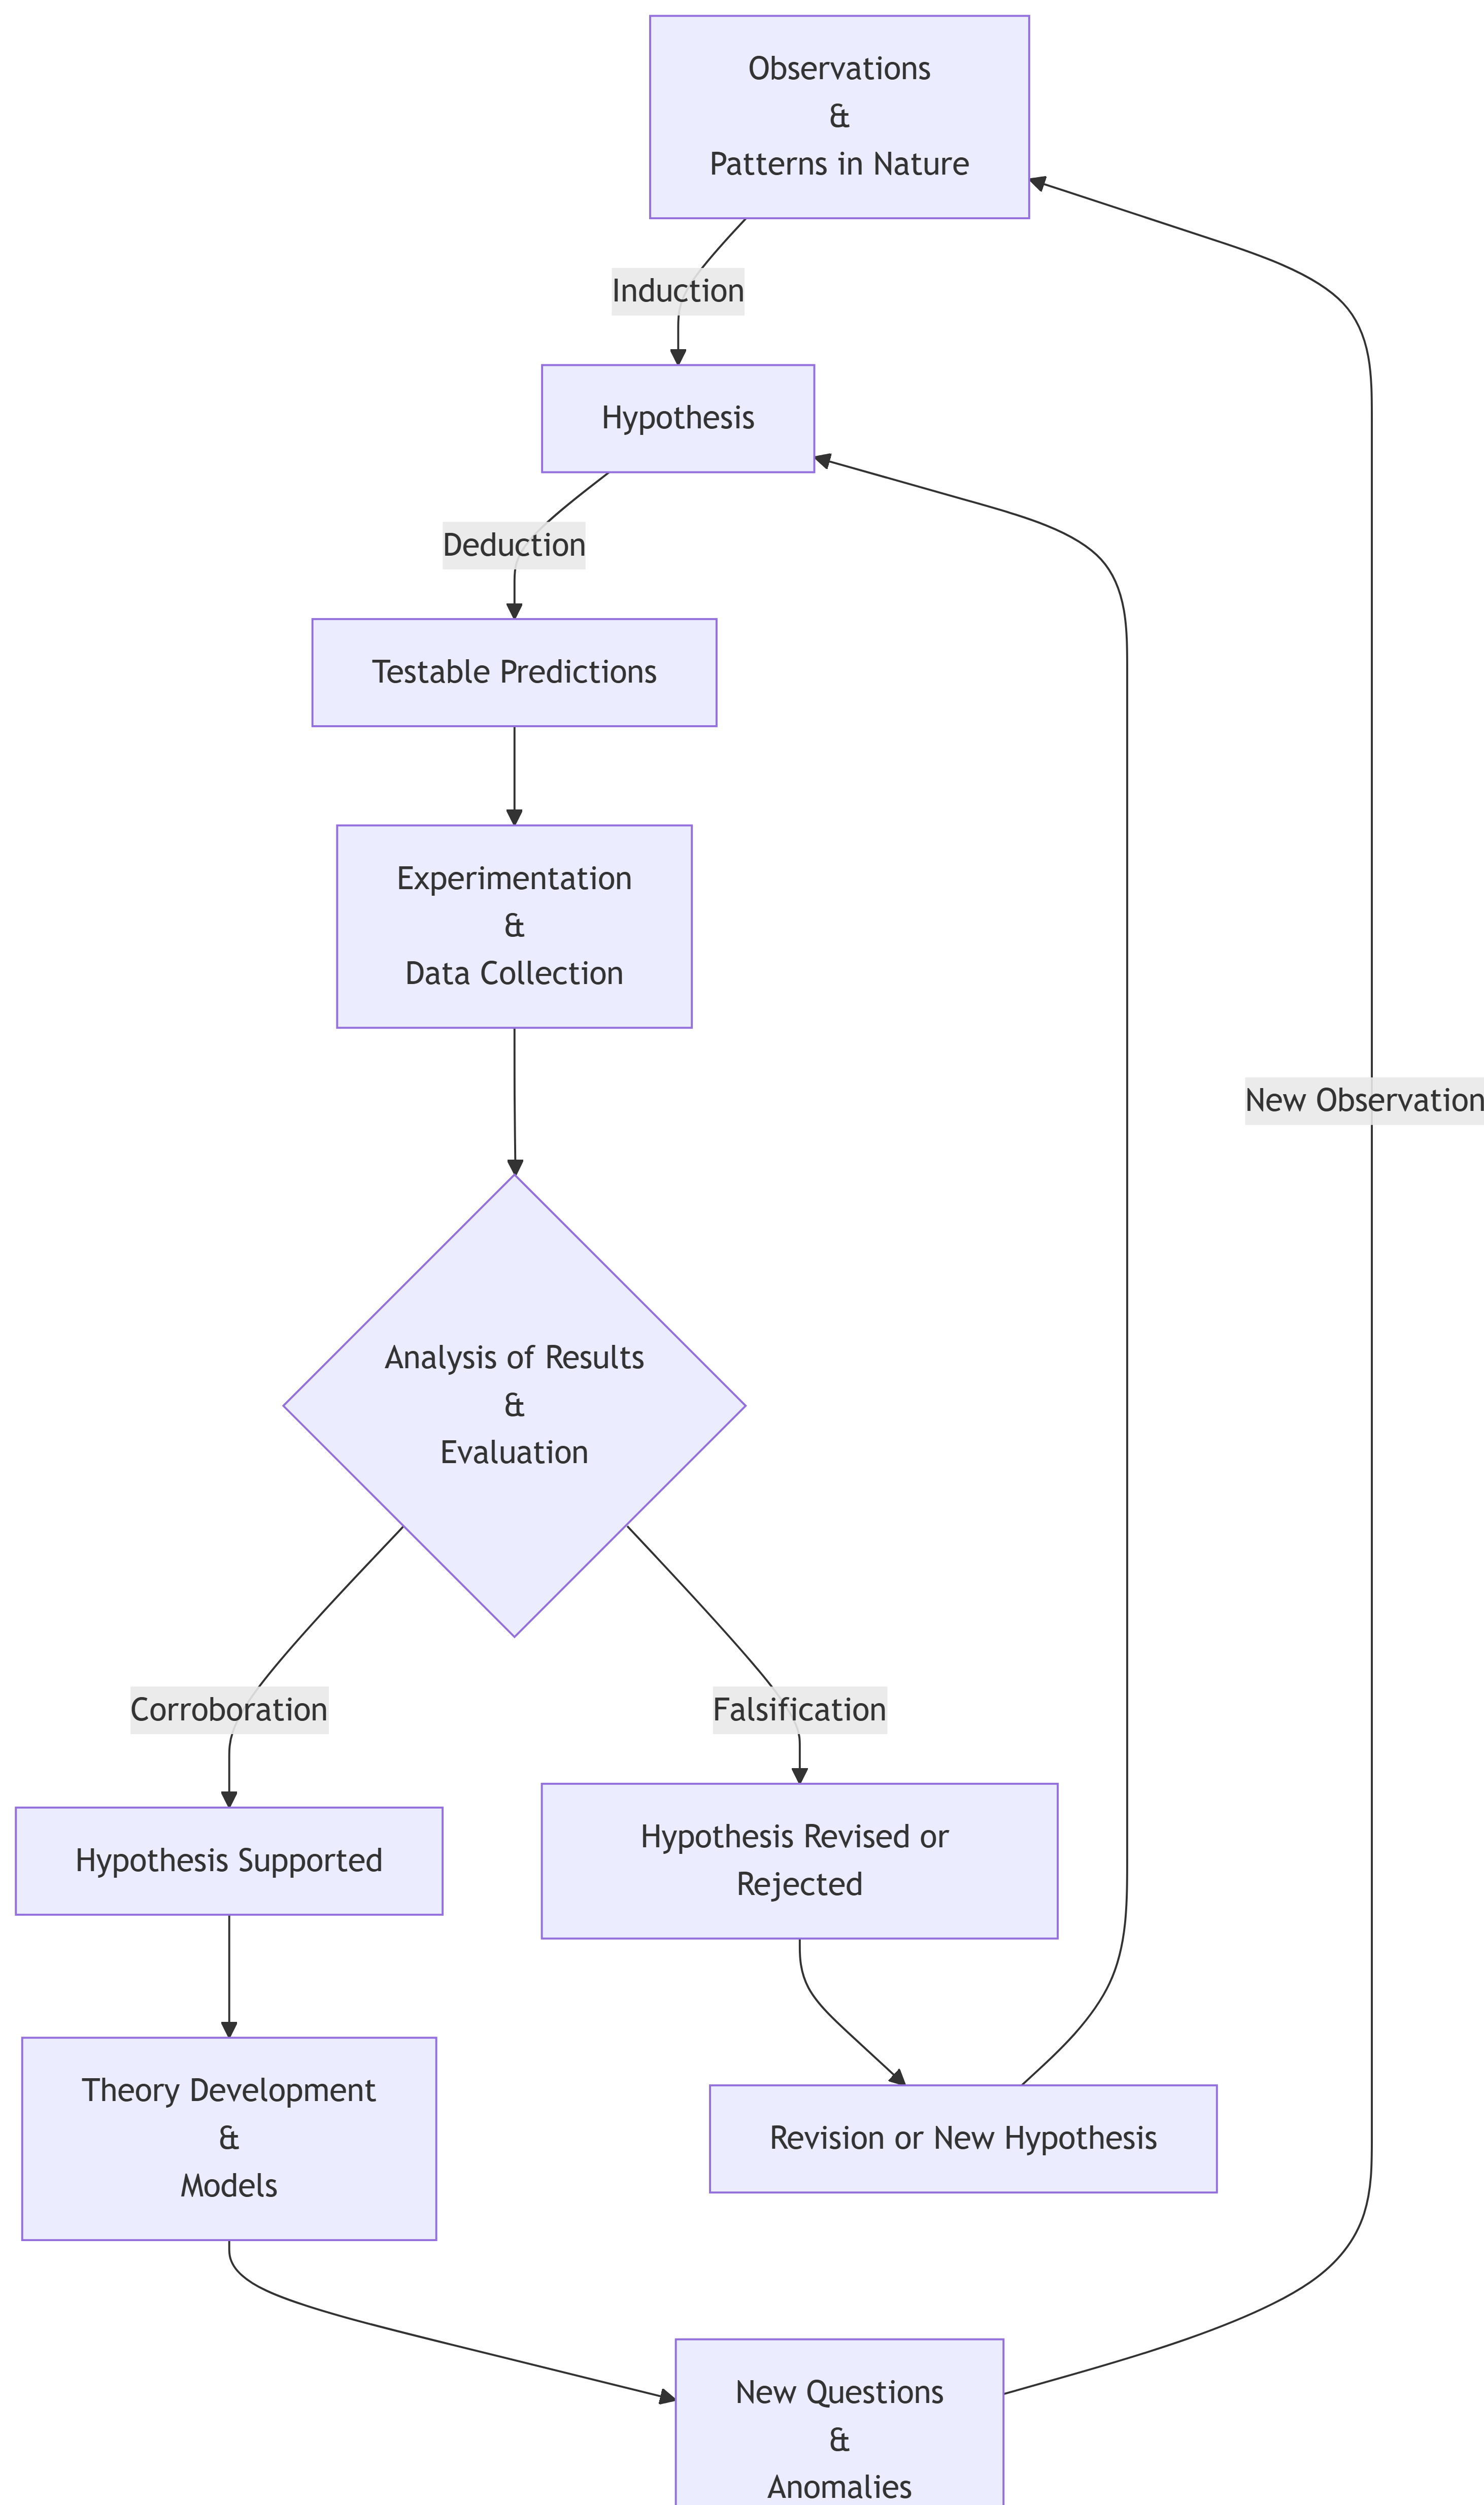
\includegraphics[width=5in,height=7in]{6-writings-and-essays/1-data-science-age-of-hype_files/figure-latex/mermaid-figure-1.png}

}

\caption{\label{fig-hd_algorithm}The hypothetico-deductive method as an
iterative loop: observations motivate hypotheses (induction); hypotheses
yield testable predictions (deduction); empirical results either support
or challenge the hypothesis, leading to theory formation or revision and
ultimately to new questions that restart the process.}

\end{figure}%

Viewed from this angle, the role of a data scientist extends far beyond
executing algorithms or statistical routines. It is the
\textbf{iterative application of the scientific method} across diverse
business contexts generating hypotheses, building predictive and causal
models, confronting them with evidence, and allowing data to arbitrate
which explanations survive. Data Science thus emerges not merely as a
technical discipline, but as the \textbf{contemporary expression of
scientific thinking} applied to data-rich environments, where
distinguishing correlation from causation and prediction from
explanation defines true professional excellence.

\section{The Fundamental Constituents of Data
Science}\label{the-fundamental-constituents-of-data-science}

Despite its rapid expansion and increasing visibility, Data Science is
often portrayed as a discipline defined by an ever-growing collection of
tools, frameworks, and technological trends. New libraries, platforms,
and modeling techniques appear constantly, creating the impression that
the field evolves primarily through technological novelty. This
perception, however, can be misleading. While modern practice indeed
relies on a rich computational ecosystem, the scientific core of Data
Science is not defined by software stacks or fashionable methodologies.
Rather, it rests on a far more compact and principled foundation:
\textbf{probabilistic reasoning and statistical inference}.

From a first-principles perspective, Data Science is best understood as
a systematic framework for reasoning under uncertainty using data.
Probability provides the language to model randomness and variability,
while Statistics supplies the methodological machinery for learning from
data and evaluating the reliability of the conclusions we draw from it.
Together, they form the conceptual backbone that allows data-driven
reasoning to remain coherent, interpretable, and scientifically
grounded.

Computation plays a crucial---but often misunderstood---role in this
framework. The term \emph{computation} derives from the Latin
\emph{computatio}, formed by the prefix \emph{com} (``together'' or
``with'') and \emph{putatio}, related to \emph{putare}, meaning ``to
calculate'' or ``to reckon.'' In its original sense, the word conveys
the idea of \textbf{calculating together}. In this light, computation
can be understood not as an autonomous source of knowledge, but as a
process through which machines assist human reasoning by carrying out
calculations at scales and speeds beyond our natural capacity.
Algorithms, programming languages, and computational environments
therefore act as instruments that enable probabilistic models to be
simulated, statistical procedures to be implemented, and empirical
hypotheses to be tested. Computation does not define Data Science; it
provides the \textbf{operational medium} through which probabilistic and
statistical reasoning becomes executable in practice.

\section{Data Science as a Strategic Value
Engine}\label{data-science-as-a-strategic-value-engine}

At this point, it is crucial to emphasize a key principle that often
gets overlooked: \textbf{Data Science is not a goal in itself}. No
matter how sophisticated the methodologies or how advanced the machine
learning models, they are worthless if they do not generate real and
measurable impact. The true purpose of Data Science is to inform and
improve strategic decisions---transforming data into outcomes that
advance organizational goals.

Data-driven decision making empowers organizations to optimize
operations, personalize customer experiences, identify risks
proactively, and maintain a competitive advantage. As Kozyrkov
highlights, outstanding data analysts ensure that their work is focused
on solving the \textbf{right business problems}, not simply producing
technically impressive outputs
\citeproc{ref-kozyrkov2018great}{{[}42{]}}.

This underscores a critical truth: technical excellence without business
alignment leads to solutions that may appear successful internally but
\textbf{fail to influence decisions or create value}. The impact of a
model is not measured solely by statistical accuracy or computational
ingenuity, but by the extent to which it \textbf{changes what the
organization does}.

From a decision-theoretic perspective, integrating Data Science into
strategy enables measurable improvements not only in profitability or
utility, but also in \textbf{decision velocity}. Automated analytical
pipelines allow organizations to deploy models directly into operational
environments continuously monitoring performance, adapting to new data,
and discarding approaches that no longer deliver value. This creates a
self-correcting loop where models are evaluated and refined over time,
accelerating the pathway from insight to action.

Consider, for example, the case of \textbf{customer churn} in retail.
Without Data Science, retention strategies typically rely on intuition
or broad marketing campaigns, often costly and ineffective. In contrast,
a churn prediction model can \textbf{identify customers most at risk},
enabling targeted interventions such as personalized offers or loyalty
programs. If the strategy does not reduce churn among the targeted
segment, performance monitoring mechanisms reveal the failure, prompting
refinement or alternative plans. Here, data does not merely describe
behavior---it actively shapes business outcomes.

Viewed through this lens, Data Science becomes a \textbf{strategic value
engine}: a discipline that leverages scientific reasoning, computational
tools, and domain expertise to drive decisions that matter. This
synthesis---model-driven insight aligned with real-world
objectives---ensures that Data Science fulfills its true mission:
transforming information into impact.

\section{Why the Scientific Method Still
Matters}\label{why-the-scientific-method-still-matters}

The strategic impact of Data Science ultimately stems from something
deeper than predictive models or analytical pipelines. Its real strength
lies in the intellectual framework that guides how data is interpreted,
hypotheses are formulated, and decisions are evaluated. The ability of
Data Science to generate meaningful impact in organizations is therefore
inseparable from the scientific principles that structure its practice.

In an era defined by rapid technological change and the constant
emergence of new tools, it is tempting to define Data Science by its
most visible artifacts: programming languages, machine learning
libraries, cloud platforms, and ever-evolving frameworks. Yet these
elements, while powerful, are ultimately transient. Technologies evolve,
tools are replaced, and methodologies shift as the field continues to
mature.

What endures is something far more fundamental: the scientific mindset
that underlies the discipline. At its core, Data Science is not about
algorithms but about \textbf{reasoning under uncertainty}, formulating
hypotheses, confronting them with data, and refining our understanding
of complex phenomena through systematic evidence. Probability provides
the language for uncertainty, statistics supplies the methods for
inference, and computation serves as the medium through which these
ideas become operational.

When practiced in this way, Data Science becomes more than a collection
of analytical techniques---it becomes a modern expression of the
scientific method applied to data-rich environments. Its true power lies
not in automation or predictive accuracy alone, but in its capacity to
transform data into knowledge and knowledge into better decisions. In
the end, the enduring value of Data Science does not come from the
sophistication of its tools, but from the rigor of the thinking that
guides their use.

The original version is available on Medium
\href{https://medium.com/@rodrigokang88/data-science-in-the-age-of-hype-4d19943f0398}{here}.

\chapter{Conformal Geometry and Electrostatics in Three
Dimensions}\label{conformal-geometry-and-electrostatics-in-three-dimensions}

\emph{Header.}

\section{Problem Definition}\label{problem-definition-12}

\emph{Section.}

\section{Modeling Approach}\label{modeling-approach-12}

\emph{Section.}

\section{Methodology and
Implementation}\label{methodology-and-implementation-12}

\emph{Section.}

\section{Results, Discussion, and
Limitations}\label{results-discussion-and-limitations-12}

\emph{Section.}

\section{Technical Appendix
(Optional)}\label{technical-appendix-optional-11}

\emph{Section.}

\section{Laplace's equation}\label{laplaces-equation}

\begin{equation}\phantomsection\label{eq-laplace-equation}{
\nabla^2 \phi = \frac{\partial ^2 \phi}{\partial x^2} +\frac{\partial ^2 \phi}{\partial y^2} + \frac{\partial ^2 \phi}{\partial z^2} = 0
}\end{equation}

\section{Conformal Mappings}\label{conformal-mappings}

\begin{figure}

\centering{

\pandocbounded{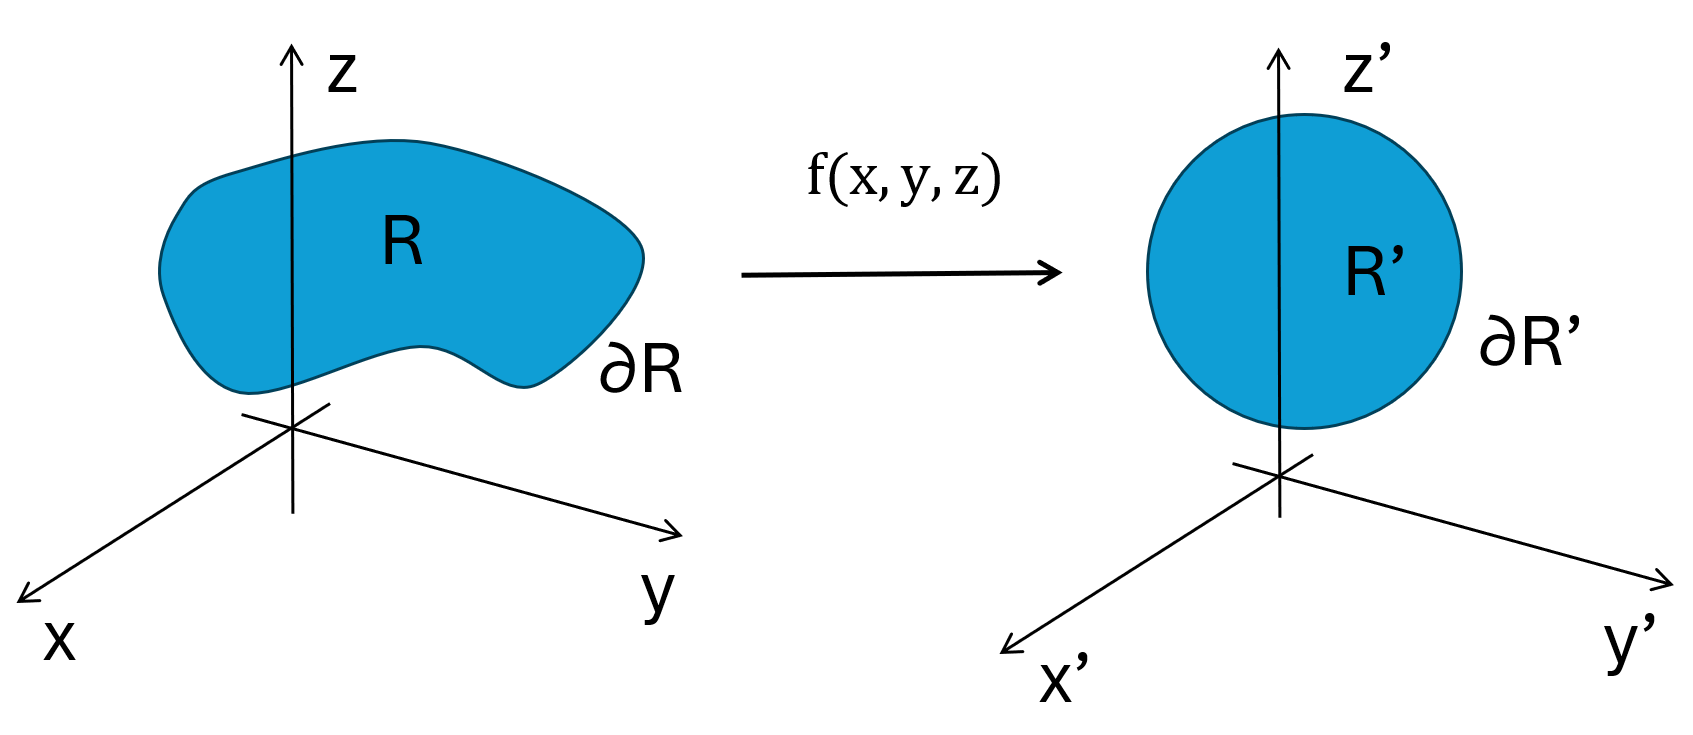
\includegraphics[keepaspectratio]{6-writings-and-essays/figures/conformal-transformation.png}}

}

\caption{\label{fig-conformal-transformation}Schematic representation of
a conformal transformation \(f(x,y,z)\) mapping a region \(R\) with
boundary \(\partial R\) in the \((x,y,z)\) coordinate system into a
transformed region \(R'\) with boundary \(\partial R'\) in the
\((x',y',z')\) coordinate system.}

\end{figure}%

As shown in Figure~\ref{fig-conformal-transformation}, \ldots{}

Suppose we have a region \(R\) in \(xyz\) space in which a scalar field
\(\phi\) satisfies Laplace's equation
Equation~\ref{eq-laplace-equation}. We want to determine what conditions
a transformation \(f: R \rightarrow R'\) must satisfy such that
Laplace's equation remains invariant under this transformation. For
simplicity, let's consider the simplest case in \(\mathbb{R}^2\).

Applying the chain rule we have that:

\begin{equation}\phantomsection\label{eq-first-derivative-chain-rule}{
\begin{aligned}
\frac{\partial \phi}{\partial x} &=
\frac{\partial \phi}{\partial x'} \frac{\partial x'}{\partial x}
+
\frac{\partial \phi}{\partial y'} \frac{\partial y'}{\partial x} \\
\frac{\partial \phi}{\partial y} &=
\frac{\partial \phi}{\partial x'} \frac{\partial x'}{\partial y}
+
\frac{\partial \phi}{\partial y'} \frac{\partial y'}{\partial y}
\end{aligned}
}\end{equation}

\bookmarksetup{startatroot}

\chapter*{References}\label{references}
\addcontentsline{toc}{chapter}{References}

\markboth{References}{References}

\phantomsection\label{refs}
\begin{CSLReferences}{0}{0}
\bibitem[\citeproctext]{ref-markowitz1952portfolio}
\CSLLeftMargin{{[}1{]} }%
\CSLRightInline{H. Markowitz, {``Portfolio selection,''} \emph{The
Journal of Finance}, vol. 7, no. 1, pp. 77--91, 1952.}

\bibitem[\citeproctext]{ref-sharpe1964capital}
\CSLLeftMargin{{[}2{]} }%
\CSLRightInline{W. F. Sharpe, {``Capital asset prices: A theory of
market equilibrium under conditions of risk,''} \emph{The journal of
finance}, vol. 19, no. 3, pp. 425--442, 1964.}

\bibitem[\citeproctext]{ref-lintner1975valuation}
\CSLLeftMargin{{[}3{]} }%
\CSLRightInline{J. Lintner, {``The valuation of risk assets and the
selection of risky investments in stock portfolios and capital
budgets,''} in \emph{Stochastic optimization models in finance},
Elsevier, 1975, pp. 131--155.}

\bibitem[\citeproctext]{ref-bossaerts2006lectures}
\CSLLeftMargin{{[}4{]} }%
\CSLRightInline{P. L. Bossaerts and B. A. Odegaard, \emph{Lectures on
corporate finance}. World Scientific Publishing Company, 2006.}

\bibitem[\citeproctext]{ref-fama1993common}
\CSLLeftMargin{{[}5{]} }%
\CSLRightInline{E. F. Fama and K. R. French, {``Common risk factors in
the returns on stocks and bonds,''} \emph{Journal of financial
economics}, vol. 33, no. 1, pp. 3--56, 1993.}

\bibitem[\citeproctext]{ref-fama1997industry}
\CSLLeftMargin{{[}6{]} }%
\CSLRightInline{E. F. Fama and K. R. French, {``Industry costs of
equity,''} \emph{Journal of financial economics}, vol. 43, no. 2, pp.
153--193, 1997.}

\bibitem[\citeproctext]{ref-brealey2011principles}
\CSLLeftMargin{{[}7{]} }%
\CSLRightInline{R. A. Brealey, S. C. Myers, and F. Allen,
\emph{Principles of corporate finance}. McGraw-Hill Education, 2011.}

\bibitem[\citeproctext]{ref-lewinson2022python}
\CSLLeftMargin{{[}8{]} }%
\CSLRightInline{E. Lewinson, \emph{Python for finance cookbook: Over 80
powerful recipes for effective financial data analysis}. Packt
Publishing Ltd, 2022.}

\bibitem[\citeproctext]{ref-james2023statistical}
\CSLLeftMargin{{[}9{]} }%
\CSLRightInline{G. James, D. Witten, T. Hastie, R. Tibshirani, and J.
Taylor, {``An introduction to statistical learning: With applications in
python,''} Springer, 2023.}

\bibitem[\citeproctext]{ref-ugarte2016probability}
\CSLLeftMargin{{[}10{]} }%
\CSLRightInline{M. D. Ugarte, A. F. Militino, and A. T. Arnholt,
\emph{Probability and statistics with r, second edition}. Taylor \&
Francis, 2016.}

\bibitem[\citeproctext]{ref-meucci2005risk}
\CSLLeftMargin{{[}11{]} }%
\CSLRightInline{A. Meucci, \emph{Risk and asset allocation}. Springer,
2005.}

\bibitem[\citeproctext]{ref-partovi2004principal}
\CSLLeftMargin{{[}12{]} }%
\CSLRightInline{M. H. Partovi, M. Caputo, \emph{et al.}, {``Principal
portfolios: Recasting the efficient frontier,''} \emph{Economics
Bulletin}, vol. 7, no. 3, pp. 1--10, 2004.}

\bibitem[\citeproctext]{ref-lopez2016building}
\CSLLeftMargin{{[}13{]} }%
\CSLRightInline{M. Lopez de Prado, {``Building diversified portfolios
that outperform out-of-sample,''} \emph{Journal of Portfolio
Management}, 2016.}

\bibitem[\citeproctext]{ref-de2018advances}
\CSLLeftMargin{{[}14{]} }%
\CSLRightInline{M. L. De Prado, \emph{Advances in financial machine
learning}. John Wiley \& Sons, 2018.}

\bibitem[\citeproctext]{ref-hastie2009elements}
\CSLLeftMargin{{[}15{]} }%
\CSLRightInline{T. Hastie, \emph{The elements of statistical learning:
Data mining, inference, and prediction}. Springer, 2009.}

\bibitem[\citeproctext]{ref-black1973pricing}
\CSLLeftMargin{{[}16{]} }%
\CSLRightInline{F. Black and M. Scholes, {``The pricing of options and
corporate liabilities,''} \emph{Journal of political economy}, vol. 81,
no. 3, pp. 637--654, 1973.}

\bibitem[\citeproctext]{ref-merton1973theory}
\CSLLeftMargin{{[}17{]} }%
\CSLRightInline{R. C. Merton, {``Theory of rational option pricing,''}
\emph{The Bell Journal of economics and management science}, pp.
141--183, 1973.}

\bibitem[\citeproctext]{ref-rubinstein2016simulation}
\CSLLeftMargin{{[}18{]} }%
\CSLRightInline{R. Y. Rubinstein and D. P. Kroese, \emph{Simulation and
the monte carlo method}. John Wiley \& Sons, 2016.}

\bibitem[\citeproctext]{ref-feynman2010quantum}
\CSLLeftMargin{{[}19{]} }%
\CSLRightInline{R. P. Feynman, A. R. Hibbs, and D. F. Styer,
\emph{Quantum mechanics and path integrals}. Courier Corporation, 2010.}

\bibitem[\citeproctext]{ref-linetsky1997path}
\CSLLeftMargin{{[}20{]} }%
\CSLRightInline{V. Linetsky, {``The path integral approach to financial
modeling and options pricing,''} \emph{Computational Economics}, vol.
11, pp. 129--163, 1997.}

\bibitem[\citeproctext]{ref-devreese2010path}
\CSLLeftMargin{{[}21{]} }%
\CSLRightInline{J. P. Devreese, D. Lemmens, and J. Tempere, {``Path
integral approach to asian options in the black -- scholes model,''}
\emph{Physica A: Statistical Mechanics and its Applications}, vol. 389,
no. 4, pp. 780--788, 2010.}

\bibitem[\citeproctext]{ref-baaquie2007quantum}
\CSLLeftMargin{{[}22{]} }%
\CSLRightInline{B. E. Baaquie, \emph{Quantum finance: Path integrals and
hamiltonians for options and interest rates}. Cambridge University
Press, 2007.}

\bibitem[\citeproctext]{ref-dal2015calibrating}
\CSLLeftMargin{{[}23{]} }%
\CSLRightInline{A. Dal Pozzolo, O. Caelen, R. A. Johnson, and G.
Bontempi, {``Calibrating probability with undersampling for unbalanced
classification.''} in \emph{SSCI}, 2015, pp. 159--166.}

\bibitem[\citeproctext]{ref-baesens2015fraud}
\CSLLeftMargin{{[}24{]} }%
\CSLRightInline{B. Baesens, V. Van Vlasselaer, and W. Verbeke,
\emph{Fraud analytics using descriptive, predictive, and social network
techniques: A guide to data science for fraud detection}. John Wiley \&
Sons, 2015.}

\bibitem[\citeproctext]{ref-dal2017credit}
\CSLLeftMargin{{[}25{]} }%
\CSLRightInline{A. Dal Pozzolo, G. Boracchi, O. Caelen, C. Alippi, and
G. Bontempi, {``Credit card fraud detection: A realistic modeling and a
novel learning strategy,''} \emph{IEEE transactions on neural networks
and learning systems}, vol. 29, no. 8, pp. 3784--3797, 2017.}

\bibitem[\citeproctext]{ref-ngai2011application}
\CSLLeftMargin{{[}26{]} }%
\CSLRightInline{E. W. Ngai, Y. Hu, Y. H. Wong, Y. Chen, and X. Sun,
{``The application of data mining techniques in financial fraud
detection: A classification framework and an academic review of
literature,''} \emph{Decision support systems}, vol. 50, no. 3, pp.
559--569, 2011.}

\bibitem[\citeproctext]{ref-al2021financial}
\CSLLeftMargin{{[}27{]} }%
\CSLRightInline{K. G. Al-Hashedi and P. Magalingam, {``Financial fraud
detection applying data mining techniques: A comprehensive review from
2009 to 2019,''} \emph{Computer Science Review}, vol. 40, p. 100402,
2021.}

\bibitem[\citeproctext]{ref-carcillo2021combining}
\CSLLeftMargin{{[}28{]} }%
\CSLRightInline{F. Carcillo, Y.-A. Le Borgne, O. Caelen, Y. Kessaci, F.
Oblé, and G. Bontempi, {``Combining unsupervised and supervised learning
in credit card fraud detection,''} \emph{Information sciences}, vol.
557, pp. 317--331, 2021.}

\bibitem[\citeproctext]{ref-robert2008database}
\CSLLeftMargin{{[}29{]} }%
\CSLRightInline{C. B. Robert, D. K. Byung, and A. N. Scott,
\emph{Database marketing: Analyzing and managing customers}. Spinger,
2008.}

\bibitem[\citeproctext]{ref-batista2022evaluate}
\CSLLeftMargin{{[}30{]} }%
\CSLRightInline{P. V. Batista, J. Laceby, and O. Evrard, {``How to
evaluate sediment fingerprinting source apportionments,''} \emph{Journal
of Soils and Sediments}, vol. 22, no. 4, pp. 1315--1328, 2022.}

\bibitem[\citeproctext]{ref-mccaffrey2011geochemical}
\CSLLeftMargin{{[}31{]} }%
\CSLRightInline{M. A. McCaffrey, D. H. Ohms, M. Werner, C. Stone, D. K.
Baskin, and B. A. Patterson, {``Geochemical allocation of commingled oil
production or commingled gas production,''} in \emph{SPE western
regional meeting}, SPE, 2011, pp. SPE--144618.}

\bibitem[\citeproctext]{ref-sandoval2022original}
\CSLLeftMargin{{[}32{]} }%
\CSLRightInline{L. Sandoval, M. Riva, P. Franco, I. Colombo, R.
Galimberti, and A. Guadagnini, {``An original deconvolution approach for
oil production allocation based on geochemical fingerprinting,''}
\emph{Fuel}, vol. 327, p. 124715, 2022.}

\bibitem[\citeproctext]{ref-tukey1962future}
\CSLLeftMargin{{[}33{]} }%
\CSLRightInline{J. W. Tukey, {``The future of data analysis,''} in
\emph{Breakthroughs in statistics: Methodology and distribution},
Springer, 1962, pp. 408--452.}

\bibitem[\citeproctext]{ref-donoho2017}
\CSLLeftMargin{{[}34{]} }%
\CSLRightInline{D. L. Donoho, {``50 years of data science,''}
\emph{Journal of Computational and Graphical Statistics}, vol. 26, no.
4, pp. 745--766, 2017.}

\bibitem[\citeproctext]{ref-naur1974concise}
\CSLLeftMargin{{[}35{]} }%
\CSLRightInline{P. Naur, \emph{Concise survey of computer methods}.
Petrocelli/Charter Books, 1974.}

\bibitem[\citeproctext]{ref-wu1997statistics}
\CSLLeftMargin{{[}36{]} }%
\CSLRightInline{C. F. J. Wu, {``Statistics = data science?''} 1997.
Available:
\url{https://www2.isye.gatech.edu/~jeffwu/presentations/datascience.pdf}}

\bibitem[\citeproctext]{ref-cleveland2001data}
\CSLLeftMargin{{[}37{]} }%
\CSLRightInline{W. S. Cleveland, {``Data science: An action plan for
expanding the technical areas of the field of statistics,''}
\emph{International Statistical Review}, vol. 69, no. 1, pp. 21--26,
2001.}

\bibitem[\citeproctext]{ref-breiman2001statistical}
\CSLLeftMargin{{[}38{]} }%
\CSLRightInline{L. Breiman, {``Statistical modeling: The two
cultures,''} \emph{Statistical Science}, vol. 16, no. 3, pp. 199--231,
2001.}

\bibitem[\citeproctext]{ref-davenport2012data}
\CSLLeftMargin{{[}39{]} }%
\CSLRightInline{T. H. Davenport and D. Patil, {``Data scientist,''}
\emph{Harvard business review}, vol. 90, no. 5, pp. 70--76, 2012.}

\bibitem[\citeproctext]{ref-johansson2016philosophy}
\CSLLeftMargin{{[}40{]} }%
\CSLRightInline{L.-G. Johansson \emph{et al.}, \emph{Philosophy of
science for scientists}. Springer, 2016.}

\bibitem[\citeproctext]{ref-klimovsky1994desventuras}
\CSLLeftMargin{{[}41{]} }%
\CSLRightInline{G. Klimovsky, \emph{Las desventuras del conocimiento
científico}. A-Z Editora, 1994.}

\bibitem[\citeproctext]{ref-kozyrkov2018great}
\CSLLeftMargin{{[}42{]} }%
\CSLRightInline{C. Kozyrkov, {``What great data analysts do---and why
every organization needs them,''} \emph{Harvard Business Review}, 2018.}

\end{CSLReferences}


\backmatter


\end{document}
